% !TEX TS-program = lualatex
% encoding : utf8 
% Documentation of tkz-elements v3.34c
% Copyright 2025  Alain Matthes
% This work may be distributed and/or modified under the
% conditions of the LaTeX Project Public License, either version 1.3
% of this license or (at your option) any later version.
% The latest version of this license is in
% http://www.latex-project.org/lppl.txt
% and version 1.3 or later is part of all distributions of LaTeX
% version 2005/12/01 or later.
% This work has the LPPL maintenance status “maintained”.
% The Current Maintainer of this work is Alain Matthes.
\PassOptionsToPackage{unicode}{hyperref}

\documentclass[DIV         = 14,
               fontsize    = 10,
               index       = totoc,
               twoside,
               cadre,
               headings    = small
               ]{tkz-doc}
\gdef\tkznameofpack{tkz-elements}
\gdef\tkzversionofpack{3.34c}
\gdef\tkzdateofpack{\today}
\gdef\tkznameofdoc{tkz-elements.pdf}
\gdef\tkzversionofdoc{3.34c}
\gdef\tkzdateofdoc{\today}
\gdef\tkzauthorofpack{Alain Matthes}
\gdef\tkzadressofauthor{}
\gdef\tkznamecollection{AlterMundus}
\gdef\tkzurlauthor{http://altermundus.fr}
\gdef\tkzengine{lualatex}
\gdef\tkzurlauthorcom{http://altermundus.fr}
\nameoffile{\tkznameofpack}

% -- Packages ---------------------------------------------------  
\usepackage[dvipsnames,svgnames]{xcolor}
\usepackage{calc}
\usepackage{tkz-base}
\usepackage[mini]{tkz-euclide}
\usepackage{tkz-elements}
\usepackage{tkzexample}
\usepackage{pgfornament}
\usetikzlibrary{backgrounds}
\usetikzlibrary{mindmap}
\usetikzlibrary{shapes.multipart}
\usepackage[colorlinks,pdfencoding=auto, psdextra]{hyperref}
\hypersetup{
      linkcolor=Gray,
      citecolor=Green,
      filecolor=Mulberry,
      urlcolor=orange,
      menucolor=Gray,
      runcolor=Mulberry,
      linkbordercolor=Gray,
      citebordercolor=Green,
      filebordercolor=Mulberry,
      urlbordercolor=NavyBlue,
      menubordercolor=Gray,
      runbordercolor=Mulberry,
      pdfsubject={Euclidean Geometry},
      pdfauthor={\tkzauthorofpack},
      pdftitle={\tkznameofpack},
      pdfcreator={\tkzengine}
}
\usepackage{unicode-math} 
\usepackage{fourier-otf}
\setmathfont{Concrete-Math.otf}
\let\rmfamily\ttfamily
\usepackage{multicol,lscape,wrapfig}
\usepackage[english]{babel}
\usepackage[normalem]{ulem}
\usepackage{multirow,multido,booktabs,cellspace}
\usepackage{shortvrb,fancyvrb,bookmark,enumitem} 
\usepackage{makeidx}
\usepackage[most]{tcolorbox}
\def\code{\texttt}
\newtcolorbox{mybox}{
enhanced,
boxrule=0pt,frame hidden,
borderline west={4pt}{0pt}{darkgray!50!white},
colback=lightgray!10!white,
sharp corners
}
%\usepackage{float}
\makeindex 

\makeatletter
\renewenvironment{theindex}
   {\section*{\indexname}\begin{multicols}{2}%
    \@mkboth{\MakeUppercase\indexname}%
  {\MakeUppercase\indexname}%
    \thispagestyle{plain}\parindent\z@
    \parskip\z@ \@plus .3\p@\relax
    \columnseprule \z@
    \columnsep 35\p@
    \let\item\@idxitem}
   {\end{multicols}}
\makeatother
\newcommand*{\tkzfname}[1]{\Amacro{#1}\textbf{\texttt{\textcolor{MidnightBlue}{%
 #1}}}}
 \newcommand*{\tkzmname}[1]{\Amacro{#1}\textbf{\texttt{\textcolor{MidnightBlue}{%
#1}}}}
 \newcommand*{\tkzaname}[1]{\Amacro{#1}\textbf{\texttt{\textcolor{MidnightBlue}{%
#1}}}}  
\def\langle{} \def\rangle{}
\renewcommand*{\IargName}[2]{\texttt{#2}\index{#1_2@\texttt{#1: argument(s)}!\texttt{#2}}}
\newcommand*{\Amacro}[1]{\index{#1_1@\texttt{#1}}}
\renewcommand*{\IoptName}[2]{\texttt{#2}\index{#1_3@\texttt{#1: attribute(s)}!\texttt{#2}}}
\newcommand*{\Iattr}[2]{\texttt{#2}\index{#1_3@\texttt{#1:  attribute}!\texttt{#2}}}
\newcommand*{\Imeth}[2]{\texttt{#2}\index{#1_3@\texttt{#1:  method}!\texttt{#2}}}
\newcommand*{\Immeth}[2]{\texttt{#2}\index{#1_3@\texttt{#1:  metamethod}!\_\_\texttt{#2}}}
\newcommand*{\Igfct}[2]{\texttt{#2}\index{#1_3@\texttt{#1:  function}!\texttt{#2}}}
\newcommand*{\Iclass}[1]{\texttt{#1}\index{Class !#1@\texttt{#1}}}
\newcommand*{\Iengine}[1]{\texttt{#1}\index{Engine !#1@\texttt{#1}}}
\newcommand*{\Iprimitive}[1]{\textbackslash\texttt{#1}\index{Lua\TeX\ primitive !#1@\texttt{\textbackslash#1}}}
\newcommand*{\tkzNameObj}[1]{\tkzname{#1}\Iobj{#1}}
\newcommand*{\Iobj}[1]{\index{Object_1@\texttt{Object}!\texttt{#1}}}
\newcommand*{\tkzRBomb}{\textcolor{red}{\bomb}}
\newcommand*{\IEmacro}[1]{\index{#1_1@\texttt{\textbackslash#1}}\texttt{#1}}
\newcommand*{\tkzimpbf}[1]{\texttt{\textbf{#1}}}
\newcommand*{\tkzEHand}{\textcolor{red}{\lefthand}}
\newcommand*{\ItkzPopt}[2]{\texttt{#2}\index{#1_3@\texttt{#1: options}!\texttt{#2}}}
%<---------------------------------------------------------------------------> 
% settings styles

\tkzSetUpColors[background=white,text=darkgray]  
\tkzSetUpPoint[size=2,color=teal,fill=teal!10]
\tkzSetUpLine[ultra thin,color=teal]
\tkzSetUpCompass[color=orange,ultra thin,/tkzcompass/delta=10] 
\tikzset{label style/.append style={below right,color=teal,font=\scriptsize}}
\tikzset{new/.style={color=orange,ultra thin}} 
\tikzset{step 1/.style={color=cyan,ultra thin}} 
\tikzset{step 2/.style={color=purple,ultra thin}} 
\def\tkzar{\hspace{1em}-->\hspace{1em}}

\makeatletter\let\percentchar\@percentchar\makeatother
\def\luaveclen#1#2{%
\directlua{tex.print(string.format(
'\percentchar.5f',math.sqrt((#1)*(#1)+(#2)*(#2))))
}}
% printnumber
\newenvironment{SVerbatim}
  {\small\Verbatim}
  {\endVerbatim}
  
\let\pmpn\pgfmathprintnumber
\AtBeginDocument{\MakeShortVerb{\|}} % link to shortvrb

\begin{document} 
  
\parindent=0pt
\tkzTitleFrame{tkz-elements \tkzversionofpack\\Euclidean Geometry}
\clearpage


\defoffile{
 This document compiles some notes about  \tkzname{\tkznameofpack}, the initial version of a \code{Lua}  library designed to perform all the necessary calculations for defining objects in Euclidean geometry figures. Your document  must be compiled using Lua\LaTeX.\\ 
 With \pkg{tkz-elements}, definitions and calculations are exclusively conducted using \pkg{Lua}. \\ 
 The main programming approach provided is object-oriented, utilizing object classes such as point, line, triangle,  and conic.  Currently, after the calculations are completed, \pkg{tkz-euclide} is used for drawing purposes. (but you can also use \TIKZ)\\
 I discovered Lua and object-oriented programming  while developing this package, so it's highly likely that I've made a few mistakes.   If you'd like to contribute to the development of this package or provide advice on how to proceed, please contact me via email.
}

\presentation

\vspace*{1cm}

\lefthand\ Acknowledgements : I received much valuable advices, remarks, corrections  from \\ \tkzimp{Nicolas Kisselhoff}, \tkzimp{David Carlisle}, \tkzimp{Roberto Giacomelli} and \tkzimp{Qrrbrbirlbel}.\\
Special thanks to \tkzimp{Wolfgang Büchel} for his invaluable contribution in correcting the examples.

\vspace*{12pt}
\lefthand\ I would also like to extend my gratitude to \tkzimp{Eric Weisstein}, creator of 
\href{http://mathworld.wolfram.com/about/author.html}{MathWorld}.

\vspace*{12pt}
\lefthand\ You can find some examples on my site and a french documentation:
\href{http://altermundus.fr}{altermundus.fr}.

\vfill
Please report typos or any other comments to this documentation to: \href{mailto:al.ma@mac.com}{\textcolor{blue}{Alain Matthes}}.

This file can be redistributed and/or modified under the terms of the \LaTeX{} 
Project Public License Distributed from \href{http://www.ctan.org/}{CTAN}\  archives.

\clearpage


\tableofcontents

\clearpage
\newpage
\section{News} % (fold)
\label{sec:news}

The documentation you are reading corresponds to the latest version (3.32c) of \tkzNamePack{tkz-elements}.
One significant feature introduced in version 3.0 was the use of the \Iprimitive{directlua} macro, replacing the \tkzNameEnv{tkzelements} environment. If you're creating documents with a large number of figures, it's a good idea to place the \code{init\_elements} function at the start of the lua code, to empty the tables. (see examples in this document)


In  version  3.10c, most functions have been optimized and a few methods are emerging. In particular, methods for determining a circle tangent to different objects. (see \ref{ssub:c_l_pp}; \ref{ssub:method_c__ll__p}; \ref{ssub:method_c__c__pp}; \ref{ssub:method_c_cc_p}; \ref{ssub:method_c_lc_p}; and \ref{ssub:tr_method_c__ll__p})

In version 3.30c, the main new feature is the introduction of the \code{conic} class, which allows you to define parabolas, hyperbolas, and ellipses. The previous \code{ellipse} class is still available but is now obsolete. This new definition is based on a focus, a directrix, and an eccentricity. Curve points are no longer entirely generated using \TIKZ{}; instead, they are computed through a geometric construction, stored in a table, and then passed to \TIKZ{} to draw the curve. This class also includes various methods, such as tangent computation and intersection with a line.

Use the \Imeth{conic}{tkzDrawCoordinates} macro to draw the curve and the \Imeth{conic}{tkzDrawPointOnCurve} macro to place a point on it.

Other important additions in this version include parallel projection onto a line and the affinity transformation.

A small change has also been made to the \code{regular\_polygon} class: the \code{table} attribute has been replaced with the more explicit \code{vertices} attribute.

Another change is the removal of scaling in the \code{lua} part. It turned out that this caused significant code management issues, while scaling with \TIKZ{} was already highly effective (since the most important calculations were already performed). From now on, scaling is not supported by certain functions, so it is recommended to use it only within the \code{tikzpicture} environment.

In version 3.32c, a change has been made to the \code{occs} class: the first argument is still a straight line, but it is no longer the directrix of a conic. Instead, it becomes the main axis passing through a vertex and a focus. This axis will serve as the future ordinate axis. This class can, of course, be used for other constructions beyond conics.

% section news (end)
\endinput


\section{Structure} % (fold)
\label{sec:structure}

The package defines  two macros |\tkzGetNodes| and |\tkzUseLua|.

Additionally, the package loads  the file |tkz_elements_main.lua|. This file initializes all the tables that will be used by the modules in which the classes are defined. In this file, a function is defined to reset all tables and the scale. This is the function \Igfct{tkz-elements}{init\_elements}.
 
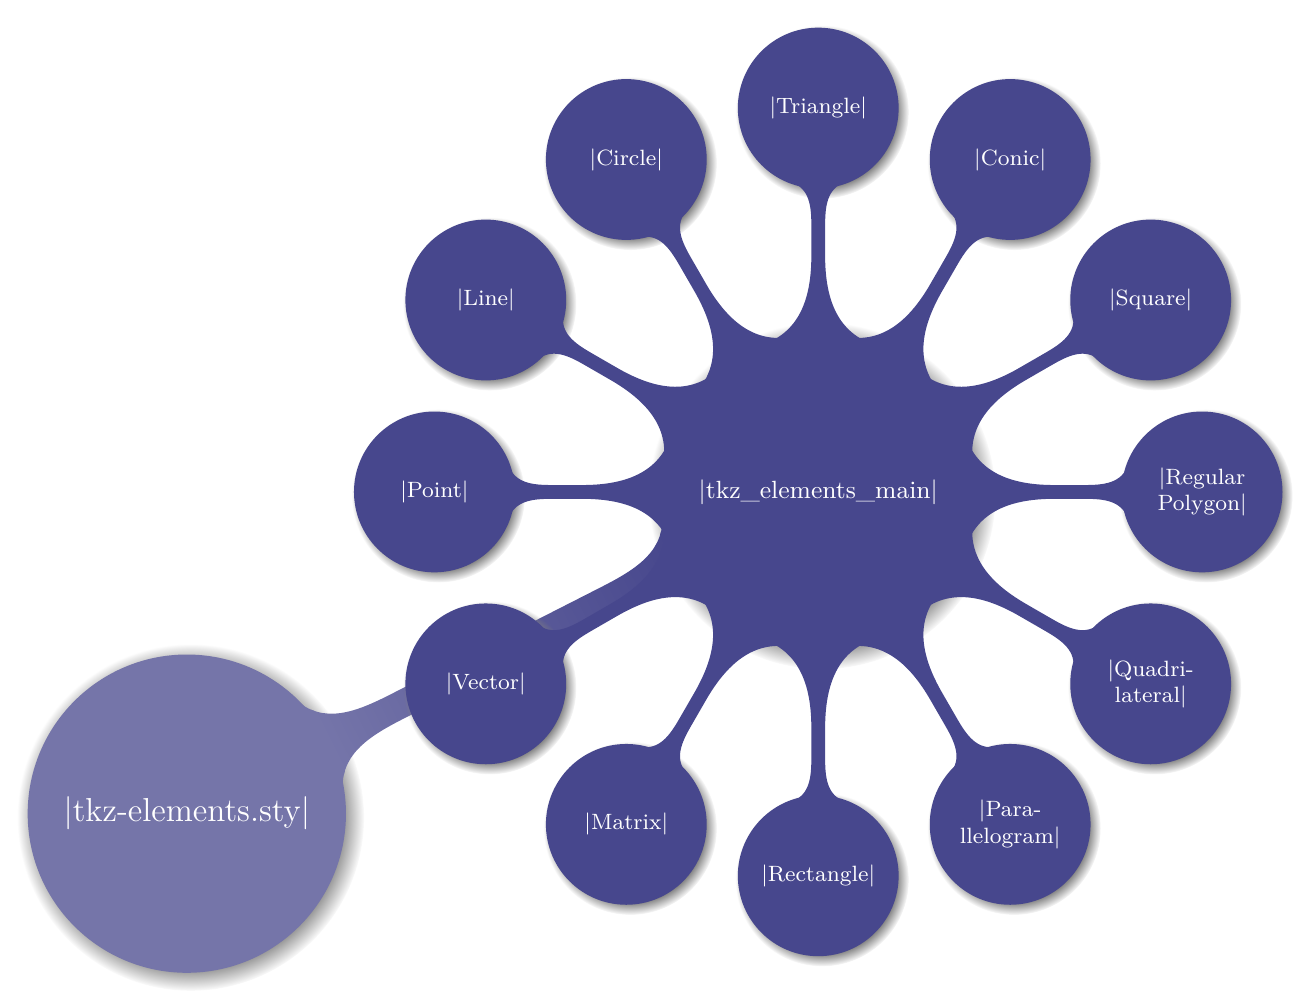
\begin{tikzpicture}[scale=.75]
\begin{scope}
\path[mindmap, concept color=MidnightBlue!60, text=white,text width=38mm,
 level 1 concept/.append style={level distance=120mm,
  sibling angle=72},
 set angles for level/.style={level 2/.append style={
 sibling angle=360/\the\tikznumberofchildren}},
 level/.append style={set angles for level=2},
 level 3 concept/.append style={level distance=20mm,
  sibling angle=20},
 L1/.style={level distance=45mm},
 L2/.style={level distance=65mm,minimum size=2cm}]

node[concept,circular drop shadow] {|tkz-elements.sty|} [clockwise from=10]

child[concept color= MidnightBlue!80,minimum size=4cm,text width=38mm,
clockwise from=27] { 
  node[concept,circular drop shadow] {|tkz\_elements\_main|} 
  [clockwise from=0]
  child[L2] { node[concept,circular drop shadow] {|Regular Polygon|} }
  child[L2] { node[concept,circular drop shadow] {|Quadri\-lateral|} }
  child[L2] { node[concept,circular drop shadow] {|Para\-llelogram|} }
  child[L2] { node[concept,circular drop shadow] {|Rectangle|} }
  child[L2] { node[concept,circular drop shadow] {|Matrix|} }
  child[L2] { node[concept,circular drop shadow] {|Vector|} }
  child[L2] { node[concept,circular drop shadow] {|Point|} }
  child[L2] { node[concept,circular drop shadow] {|Line|} }
  child[L2] { node[concept,circular drop shadow] {|Circle|} }
  child[L2] { node[concept,circular drop shadow] {|Triangle|} }
  child[L2] { node[concept,circular drop shadow] {|Conic|} }
  child[L2] { node[concept,circular drop shadow] {|Square|} }
};
\end{scope}
\end{tikzpicture}

The current classes are :

 \Iclass{point} (z) ;  \Iclass{line} (L) ; \Iclass{circle} (C) ; \Iclass{triangle} (T) ; \Iclass{conic} (E) ; \Iclass{quadrilateral} (Q) ; \Iclass{square} (S) ; \Iclass{rectangle} (R) ; \Iclass{parallelogram} (P) ; \Iclass{regular\_polygon} (RP); \Iclass{vector} (V) and \Iclass{matrix} (M).
   


If |name| is name of a class, you can find its definition in the file |tkz_elements_name.lua|.

     
% section structure (end)



\newpage
\section{Why tkz-elements?} % (fold)
\label{sec:why_tkz_elements}

\subsection{Calculation accuracy} % (fold)
\label{sub:calculation_accuracy}

\subsubsection{Calculation accuracy in \TIKZ} % (fold)
\label{ssub:calculation_accuracy_in_tikz}

With \TIKZ,  the expression \tkzimp{|veclen(x,y)|} calculates the expression $\sqrt{x^2+y^2}$.
This calculation is achieved through a polynomial approximation, drawing inspiration from the ideas  of \tkzimp{Rouben Rostamian}.

\pgfkeys{/pgf/number format/.cd,std,precision=5} \pgfmathparse{veclen(65,72)} 
\begin{mybox}{}
\begin{Verbatim}
   pgfmathparse{veclen(65,72)} \pgfmathresult
\end{Verbatim}
\end{mybox}

 \tkzHand $\sqrt{65^2+72^2} \approx \pmpn{\pgfmathresult} $ \tkzRBomb.
% subsubsection calculation_accuracy_in_tikz (end)

\subsubsection{Calculation accuracy in Lua} % (fold)
\label{ssub:calculation_accuracy_in_lua}

A |luaveclen| macro can be defined as follows:

\begin{mybox}{}
\begin{Verbatim}
\def\luaveclen#1#2{\directlua{tex.print(string.format(
'\percentchar.5f',math.sqrt((#1)*(#1)+(#2)*(#2))))}}
\end{Verbatim}
\end{mybox}

and

\begin{mybox}
\begin{Verbatim}
\luaveclen{65}{72}
\end{Verbatim}
\end{mybox}

gives 
\tkzHand $\sqrt{65^2+72^2} = \pmpn{\luaveclen{65}{72}} $ {\color{red}!!}

The error, though insignificant when it comes to the placement of an object on a page by a hundredth of a point, becomes problematic for the results of mathematical demonstrations. Moreover, these inaccuracies can accumulate and lead to erroneous constructions.

\vspace{.5em}
To address this lack of precision, I initially introduced the \pkg{fp}, followed by the package \pkg{xfp}. More recently, with the emergence of Lua\LATEX{}, I incorporated a \tkzname{Lua} option aimed at performing calculations with \tkzname{Lua}.

This was the primary motivation behind creating the package, with the secondary goal being the introduction of object-oriented programming (OOP) and simplifying programming with Lua. The concept of OOP persuaded me to explore its various possibilities further.

At that time, I had received some Lua programming examples from {\tkzimpbf{Nicolas Kisselhoff}}, but I struggled to understand the code initially, so I dedicated time to studying Lua patiently. Eventually, I was able to develop \tkzname{\tkznameofpack}, incorporating many of his ideas that I adapted for the package.


% subsubsection calculation_accuracy_in_lua (end)
\subsubsection{Using objects} % (fold)
\label{ssub:using_objects}

Subsequently, I came across an article by \tkzimpbf{Roberto Giacomelli}\footnote{\href{https://www.guitex.org/home/images/meeting2012/slides/presentazione_giacomell_guitmeeting_2012.pdf}{Grafica ad oggetti con LuaTEX}}  on object-oriented programming using \tkzname{Lua} and \TIKZ\ tools. This served as my second source of inspiration.   Not only did this approach enable programming to be executed step-by-step, but the introduction of objects facilitated a direct link between the code and geometry. As a result, the code became more readable, explicit, and better structured.
 
\subsubsection{Example: Apollonius circle} % (fold)
\label{ssub:example_apollonius_circle}

\begin{mybox}{Problem:}
The objective is to identify an inner tangent circle to the three exinscribed circles of a triangle.\end{mybox}

 For additional details, refer to \href{https://mathworld.wolfram.com/ApolloniusCircle.html}{MathWorld} for more details.

This example served as my reference for testing the \pkg{tkz-euclide} package. Initially, with my first methods and the tools available to me, the results lacked precision.  However, with tkz-elements, I now have access to more powerful and precise tools that are also easier to use.

The fundamental principles of figure construction with \tkzname{tkz-euclide} remain intact: definitions, calculations, tracings, labels, as well as the  step-by-step programming, mirroring the process of construction with a ruler and compass. 

This version utilizes the simplest construction method made possible by Lua.

\begin{mybox}
\begin{Verbatim}
\directlua{
  z.A             = point: new (0,0)
  z.B             = point: new (6,0)
  z.C             = point: new (0.8,4)
  T.ABC           = triangle : new ( z.A,z.B,z.C )
  z.N             = T.ABC.eulercenter
  z.S             = T.ABC.spiekercenter
  T.feuerbach     = T.ABC : feuerbach ()
  z.Ea,z.Eb,z.Ec  = get_points ( T.feuerbach )
  T.excentral     = T.ABC : excentral ()
  z.Ja,z.Jb,z.Jc  = get_points ( T.excentral )
  C.JaEa          = circle: new (z.Ja,z.Ea)
  C.ortho         = circle: radius (z.S,math.sqrt(C.JaEa: power(z.S)))
  z.a             = C.ortho.through
  C.euler         = T.ABC: euler_circle ()
  C.apo           = C.ortho : inversion (C.euler)
  z.O             = C.apo.center
  z.xa,z.xb,z.xc  = C.ortho : inversion (z.Ea,z.Eb,z.Ec)
}
\end{Verbatim}
\end{mybox}

The creation of an object encapsulates its attributes (its characteristics) and methods (i.e. the actions that are specific to it). Subsequently, it is assigned a reference (a name) which is linked to the object using a table. This table functions as an associative array that links the reference, called a \tkzimp{key}, to a \tkzimp{value}, in this case, the object. Further elaboration on these notions will be provided later.

For instance, let \tkzimp{T} be a table associating the object \tkzimp{triangle} with the key \tkzimp{ABC}. \tkzimp{T.ABC} is also a table, and its elements are accessed using keys that correspond to attributes of the triangle. These attributes have been defined within the package.

\vspace{1em}
\begin{mybox}
\begin{Verbatim}
 z.N = T.ABC.eulercenter 
\end{Verbatim}
\end{mybox}

|N| is the name of the point, |eulercenter| is an attribute of the triangle.
\footnote{ The center of the Euler circle, or center of the nine-point circle, is a characteristic of every triangle.}

\begin{mybox}
\begin{Verbatim}
 T.excentral     = T.ABC : excentral () 
\end{Verbatim}
\end{mybox}

In this context, \tkzimp{excentral} is a method associated with the \tkzimp{T.ABC }object. It defines the triangle formed by the centers of the exinscribed circles. 

Of particular importance are two lines of code. The first one below demonstrates that the exceptional precision provided by Lua allows for the definition of a radius through a complex calculation.  The radius of the radical circle is determined by $\sqrt{\Pi(S,\mathcal{C}(Ja,Ea))}$ (square root of the power of point $S$ with respect to the exinscribed circle with center |Ja| passing through |Ea|). 

\begin{mybox}{}
\begin{Verbatim}
  C.ortho  = circle: radius (z.S,math.sqrt(C.JaEa: power(z.S)))
\end{Verbatim}
\end{mybox}

Lastly, it's worth noting that the inversion of the Euler circle with respect to the radical circle yields the Apollonius circle\footnote{The nine-point circle, or Euler circle, is externally tangent to the three circles. The points of tangency form Feuerbach's triangle.}. This transformation requires an object as a parameter, which is recognized by its type (all objects are typed in the package), and the method determines which algorithm to use according to this type.

\begin{mybox}{}
\begin{Verbatim}
  C.apo   = C.ortho : inversion (C.euler) 
\end{Verbatim}
\end{mybox}

Now that all the points have been defined, it's time to start drawing the paths. To accomplish this, nodes need to be created. This is the role of the macro \Imacro{tkzGetNodes}. Refer to \ref{ssub:points_transfer}

The subsequent section exclusively deals with drawings, and is managed by \pkg{tkz-euclide}.

\begin{Verbatim}
\begin{tikzpicture}
   \tkzGetNodes
   \tkzFillCircles[green!30](O,xa)
   \tkzFillCircles[teal!30](Ja,Ea Jb,Eb Jc,Ec)
   \tkzFillCircles[lightgray](S,a)
   \tkzFillCircles[green!30](N,Ea)
   \tkzDrawPoints(xa,xb,xc)
   \tkzDrawCircles(Ja,Ea Jb,Eb Jc,Ec S,a O,xa N,Ea)
   \tkzClipCircle(O,xa)
   \tkzDrawLines[add=3 and 3](A,B A,C B,C)
   \tkzDrawPoints(O,A,B,C,S,Ea,Eb,Ec,N)
   \tkzDrawSegments[dashed](S,xa S,xb S,xc)
   \tkzLabelPoints(O,N,A,B)
   \tkzLabelPoints[right](S,C)
\end{tikzpicture}
\end{Verbatim}

\vspace{1em}
\directlua{
  z.A             = point: new (0,0)
  z.B             = point: new (6,0)
  z.C             = point: new (0.8,4)
  T.ABC           = triangle : new ( z.A,z.B,z.C )
  z.N             = T.ABC.eulercenter
  z.S             = T.ABC.spiekercenter
  T.feuerbach     = T.ABC : feuerbach ()
  z.Ea,z.Eb,z.Ec  = get_points ( T.feuerbach )
  T.excentral     = T.ABC : excentral ()
  z.Ja,z.Jb,z.Jc  = get_points ( T.excentral )
  C.JaEa          = circle: new (z.Ja,z.Ea)
  C.ortho         = circle: radius (z.S,math.sqrt(C.JaEa: power(z.S)))
  z.a             = C.ortho.through
  C.euler         = T.ABC: euler_circle ()
  C.apo           = C.ortho : inversion (C.euler)
  z.O             = C.apo.center
  z.xa,z.xb,z.xc  = C.ortho : inversion (z.Ea,z.Eb,z.Ec)
}
\begin{minipage}{\textwidth}

\begin{center}
  \begin{tikzpicture}[ scale  = .4]
     \tkzGetNodes
     \tkzFillCircles[green!30](O,xa)
     \tkzFillCircles[teal!30](Ja,Ea Jb,Eb Jc,Ec)
     \tkzFillCircles[lightgray](S,a)
     \tkzFillCircles[green!30](N,Ea)
     \tkzDrawPoints(xa,xb,xc)
     \tkzDrawCircles(Ja,Ea Jb,Eb Jc,Ec S,a O,xa N,Ea)
     \tkzClipCircle(O,xa)
     \tkzDrawLines[add=3 and 3](A,B A,C B,C)
     \tkzDrawPoints(O,A,B,C,S,Ea,Eb,Ec,N)
     \tkzDrawSegments[dashed](S,xa S,xb S,xc)
     \tkzLabelPoints(O,N,A,B)
     \tkzLabelPoints[right](S,C)
  \end{tikzpicture}
\end{center}

 
\end{minipage}

% subsubsection example_apollonius_circle (end)
% subsubsection using_objects (end)
% subsection calculation_accuracy (end)
% section why_tkz_elements (end)
\newpage
\section{Presentation}

\subsection{With Lua} % (fold)
\label{sub:with_lua}

The primary function of tkz-elements is to calculate dimensions and define points, which is achieved using Lua. You can view  tkz-elements as a kernel that is utilized either by tkz-euclide or by TikZ. The lua code can be implemented immediately using the \tkzcname{directlua} primitive, or it can take place within a \tkzNameEnv{tkzelements} environment which is based on \tkzNameEnv{luacode}. In the latter case, you need to load the \pkg{luacode} package. In the first case, if you create a complex document, you'll be able to reset the tables and scale with the \Igfct{package}{init\_elements} function. 

\begin{minipage}[t]{.52\textwidth}\vspace{0pt}%
   The key points are: 
   \begin{itemize}
      \item The source file must be \tkzEHand\ {\color{red}\uline{ \color{black}UTF8}}  encoded.
      \item Compilation is done with  \tkzEHand\ {\color{red}\uline{ \color{black}Lua\LATEX{}}}.
      \item You need to load \tkzimp{\TIKZ}{} or \tkzimp{tkz-euclide} and \tkzimp{tkz-elements}.
      \item Definitions and calculations are performed in an (orthonormal) Cartesian coordinate system, using Lua with the macro \tkzcname{directlua} or within the  \tkzimp{tkzelements} environment.
   \end{itemize}
   
 On the right, you can see the minimum template.
  
The code is divided into two parts, represented by lua code, argument to the primitive |\directlua|  and the environment \tkzNameEnv{tikzpicture}. In the first part, you place your Lua code, while in the second, you use tkz-euclide commands. The \code{mini} option for \code{tkz-euclide} is used to load only the macros required for drawing. In the \code{lua} code, it is preferable to systematically use the \code{init\_elements ()} function, which cleans up the tables and re-sets \code{scale} to 1. Reminder: from now on, no scaling should be performed in the \code{lua} part.

\vspace*{4.1 cm}%
\end{minipage}\hspace*{\fill}
\begin{minipage}[t]{.45\textwidth}\vspace{0pt}%
\begin{mybox}
\begin{Verbatim}
% !TEX TS-program = lualatex
% Created by Alain Matthes
\documentclass{standalone} 
\usepackage[mini]{tkz-euclide}
% or simply TikZ
\usepackage{tkz-elements}
begin{document} 
    
\directlua{
init_elements()
% definition of some points
z.A = point : new (   ,   )
z.B = point : new (   ,   )

 ...code...
}

\begin{tikzpicture}
% point transfer to Nodes
\tkzGetNodes

\end{tikzpicture}
\end{document}
\end{Verbatim}
\end{mybox}
\end{minipage}
% subsection with_lua (end)

\subsection{The main process} % (fold)
\label{sub:the_main_process}

\tikzset{concept/.append style={fill={none}}}
\tikzset{root concept/.style=   {minimum size=3cm,text width=2.8cm}}%
\tikzset{level 1 concept/.append style={minimum size=4cm, font=\large, text width=3cm}}%
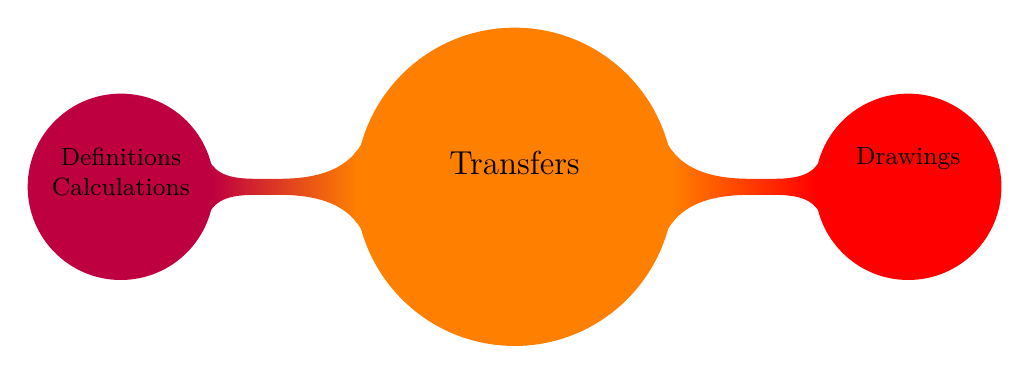
\begin{tikzpicture}
  \path[mindmap,concept color=orange,text=black]
    node[concept] {Transfers\\\textcolor{orange}{ \textbackslash{tkzGetNodes}}}
    child[concept color=red,grow=right] {
      node[concept] {Drawings\\\textcolor{red}{tkz-euclide}\\\textcolor{red}{\TIKZ}} }
    child[concept color=purple,grow=left] { 
    node[concept] {Definitions\\Calculations\\\textcolor{purple}{tkz-elements}} };
\end{tikzpicture}

After obtaining all the necessary points for the drawing, they must be transformed into \tkzname{nodes} so that \pkg{TikZ} or \pkg{tkz-euclide} can render the figure. This is accomplished using the macro \tkzcname{tkzGetNodes}. This macro iterates through  all the elements of the table |z| using the key (which is essentially the name of the point) and retrieves the associated values, namely the coordinates of the point (node).
% subsection the_main_process (end)

\subsection{Complete example: Pappus circle} % (fold)
\label{sub:the_figure_pappus_circle}

\subsubsection{The figure} 

\directlua{
z.A = point:new(0, 0)
z.B = point:new(10, 0)
L.AB = line:new(z.A, z.B)
z.C = L.AB:gold_ratio()
L.AC = line:new(z.A, z.C)
L.CB = line:new(z.C, z.B)
L.AB = line:new(z.A, z.B)
z.O_0 = L.AB.mid
z.O_1 = L.AC.mid
z.O_2 = L.CB.mid
C.AB = circle:new(z.O_0, z.B)
C.AC = circle:new(z.O_1, z.C)
C.CB = circle:new(z.O_2, z.B)
z.P = C.CB.north
z.Q = C.AC.north
z.O = C.AB.south
z.c = z.C:north(2)
C.PC = circle:new(z.P, z.C)
C.QA = circle:new(z.Q, z.A)
z.P_0 = intersection(C.PC, C.AB)
z.P_1 = intersection(C.PC, C.AC)
_, z.P_2 = intersection(C.QA, C.CB)
T.P = triangle:new(z.P_0, z.P_1, z.P_2)
z.O_3 = T.P.circumcenter
}

\begin{center}
\begin{tikzpicture}[scale = .75]
 \tkzGetNodes
 \tkzDrawCircle[black,fill=yellow!20,opacity=.4](O_0,B)
 \tkzDrawCircles[teal,fill=teal!40,opacity=.6](O_1,C O_2,B)
 \tkzDrawCircle[purple,fill=purple!20,opacity=.4](O_3,P_0)
 \tkzDrawArc[cyan,delta=10](Q,A)(P_0)
 \tkzDrawArc[cyan,delta=10](P,P_0)(B)
 \tkzDrawArc[cyan,delta=10](O,B)(A)
 \tkzDrawPoints(A,B,C,O_0,O_1,O_2,P,Q,P_0,P_0,P_1,P_2,O)
 \tkzLabelPoints(A,B,C,O_0,O_1,O_2,P,Q,P_0,P_0,P_1,P_2,O)
\end{tikzpicture}
\end{center}


% subsection the_figure_pappus_circle (end)

\subsubsection{The code} % (fold)
\label{ssub:the_code}

\begin{SVerbatim}
% !TEX TS-program = lualatex
\documentclass{article}
\usepackage{tkz-euclide}
\usepackage{tkz-elements}
\begin{document}

\directlua{
init_elements()
z.A  = point:new(0, 0)
z.B = point:new(10, 0)  %  creation of two fixed points $A$ and $B$
L.AB = line:new(z.A, z.B)
z.C = L.AB:gold_ratio()       %  use of a method linked to “line”
z.O_0 = line:new(z.A, z.B).mid % midpoint of segment with an attribute of “line”
z.O_1 = line:new(z.A, z.C).mid %  objects are not stored and cannot be reused.
z.O_2 = line:new(z.C, z.B).mid   
C.AB = circle:new(z.O_0, z.B)  %  new object “circle” stored and reused
C.AC = circle:new(z.O_1, z.C) 
C.CB = circle:new(z.O_2, z.B)
z.P = C.CB.north            %  “north” atrributes of a circle
z.Q = C.AC.north
z.O = C.AB.south
z.c = z.C:north(2)   %“north” method of a point (needs a parameter)
C.PC = circle:new(z.P, z.C)
C.QA = circle:new(z.Q, z.A)
z.P_0 = intersection(C.PC,C.AB)   %  search for intersections of two circles.
z.P_1 = intersection(C.PC,C.AC)   %   idem
_,z.P_2 = intersection(C.QA,C.CB)   %  idem
T.P = triangle:new(z.P_0, z.P_1, z.P_2)
z.O_3 = T.P.circumcenter  % circumcenter attribute of “triangle”
}
\end{SVerbatim}

\begin{SVerbatim}
\begin{tikzpicture}
  \tkzGetNodes
  \tkzDrawCircle[black,fill=yellow!20,opacity=.4](O_0,B)
  \tkzDrawCircles[teal,fill=teal!40,opacity=.6](O_1,C O_2,B)
  \tkzDrawCircle[purple,fill=purple!20,opacity=.4](O_3,P_0)
  \tkzDrawArc[cyan,delta=10](Q,A)(P_0)
  \tkzDrawArc[cyan,delta=10](P,P_0)(B)
  \tkzDrawArc[cyan,delta=10](O,B)(A)
  \tkzDrawPoints(A,B,C,O_0,O_1,O_2,P,Q,P_0,P_0,P_1,P_2,O)
  \tkzLabelPoints(A,B,C,O_0,O_1,O_2,P,Q,P_0,P_0,P_1,P_2,O)
\end{tikzpicture}
\end{document}
\end{SVerbatim}
% subsubsection the_code (end)

\subsection{Another example with comments: South Pole} % (fold)
\label{sub:south_pole}

Here's another example with comments

\begin{SVerbatim}
% !TEX TS-program = lualatex
\documentclass{standalone}
\usepackage[mini]{tkz-euclide}
\usepackage{tkz-elements}
\begin{document}
\directlua{
init_elements()
z.A = point:new(2, 4)
z.B = point:new(0, 0)               % three fixed points are used
z.C = point:new(8, 0)               %
T.ABC = triangle:new(z.A, z.B, z.C) % we create a new triangle object
C.ins = T.ABC:in_circle()           % we get the incircle of this triangle
z.I = C.ins.center                  % center is an attribute of the circle
z.T = C.ins.through                 % through is also an attribute
z.I, z.T = get_points(C.ins)        % get_points is a shortcut
C.cir = T.ABC:circum_circle()       % we get the  circumscribed circle
z.W = C.cir.center                  % we get the center of this circle
z.O = C.cir.south                   % now we get the south pole of this circle
L.AO = line:new(z.A, z.O)           % we create an object "line"
L.BC = T.ABC.bc                     % we get the line (BC)
z.I_A = intersection(L.AO, L.BC)    % we search the intersection of the last lines
}
\end{SVerbatim}

\directlua{
 init_elements()
 z.A = point:new(2, 4)
 z.B = point:new(0, 0)
 z.C = point:new(8, 0)
 T.ABC = triangle:new(z.A, z.B, z.C)
 C.ins = T.ABC:in_circle()
 z.I = C.ins.center
 z.T = C.ins.through
 C.cir = T.ABC:circum_circle()
 z.W = C.cir.center
 z.O = C.cir.south
 L.AO = line:new(z.A, z.O)
 L.BC = T.ABC.bc
 z.I_A = intersection(L.AO, L.BC)
}

\begin{center}
  \begin{tikzpicture}[ scale= 1.2]
  \tkzGetNodes
  \tkzDrawCircles(W,A I,T)
  \tkzDrawArc(O,C)(B)
  \tkzDrawPolygon(A,B,C)
  \tkzDrawSegments[new](A,O B,O C,O)
  \tkzDrawLine(B,I)
  \tkzDrawPoints(A,B,C,I,I_A,W,O)
  \tkzFillAngles[green!20,opacity=.3](A,O,B A,C,B)
  \tkzFillAngles[teal!20,opacity=.3](O,B,C B,C,O B,A,O O,A,C)
  \tkzLabelPoints(I,I_A,W,B,C,O)
  \tkzLabelPoints[above](A)
  \end{tikzpicture}
\end{center}



\vspace{12pt}
Here's the tikzpicture environment to obtain the drawing:
\begin{SVerbatim}
\begin{tikzpicture}
\tkzGetNodes
\tkzDrawCircles(W,A I,T)
\tkzDrawArc(O,C)(B)
\tkzDrawPolygon(A,B,C)
\tkzDrawSegments[new](A,O B,O C,O)
\tkzDrawLine(B,I)
\tkzDrawPoints(A,B,C,I,I_A,W,O)
\tkzFillAngles[green!20,opacity=.3](A,O,B A,C,B)
\tkzFillAngles[teal!20,opacity=.3](O,B,C B,C,O B,A,O O,A,C)
\tkzLabelPoints(I,I_A,W,B,C,O)
\tkzLabelPoints[above](A)
\end{tikzpicture}
\end{SVerbatim}
% subsection south_pole (end)
\endinput
\newpage

\section{Writing Convention} % (fold)
\label{sec:writing_convention}

\subsection{Miscellaneous} % (fold)
\label{sub:miscellanous}

\begin{itemize}
  \item As with tkz-euclide, the chosen unit is the centimeter, and by default, points are located in an orthonormal Cartesian coordinate system.
  
   \item Numerical variable: the writing conventions for real numbers are the same as for \pkg{Lua}.
   \item Complex numbers: Similar to real numbers, but to define them, you must write |za = point (1,2)|. Mathematically, this corresponds to 1+2i, which you can find with |tex.print(tostring(za))|.(Refer \ref{sub:complex_numbers})
   \item Boolean: you can write |bool = true| or |bool = false| then with Lua you can use the code :\\
 \begin{mybox}
|if bool == ... then ... else ... end|
\end{mybox}
 
 and  you can use the macro 
\begin{mybox}
 |\ifthenelse{\equal{\tkzUseLua{bool}}{true}}{ ... }{ ... }|
\end{mybox}

     after loading the \tkzNamePack{ifthen} package.
   
   \item String: if st = "Euler's formula" then \begin{mybox}
      |\tkzUseLua{st}| gives |Euler's formula|
   \end{mybox}
   

\end{itemize}
% subsection miscellanous (end)

\subsection{Assigning a Name to a Point} % (fold)
\label{sub:assigning_a_name_to_a_point}

At present,  the only obligation is to store the points in the table |z| \footnote{To place the point M in the table, simply write |z.M| = \ldots or |z["M"]|= \ldots} if you intend to use them in \TIKZ\ or \pkg{tkz-euclide}. f a point will not be used, you can designate it as you wish while adhering to Lua conventions. 

 Points in the lua code must follow a convention in the form |z.name|, where  |name| represents the name of the corresponding \tkzname{node}.
 
As for the conventions for designating |name| you must adhere to Lua conventions in particular cases.
\begin{enumerate}

   \item  The use of prime can be problematic. If the point name contains more than one symbol and ends with |p|  then when passing into \pkg{tkz-euclide}, the letters |p|  will be replaced by |'| using the macro \tkzcname{tkzGetNodes}; \index{prime}

   \item  Alternatively, for a more explicit code, suppose you want to designate a point as  "euler". You could, for example,  write |euler = ...|, and at the end of the code for the transfer, |z.E = euler|. It is also possible to use a temporary name |euler| and to replace it in \TIKZ{}. Either at the time of placing the labels, or for example by using |pgfnodealias{E}{euler}|. This possibility also applies in other cases: prime, double prime, etc.
\end{enumerate}


Here are some different ways of naming a point:
\begin{mybox}
\begin{itemize}
   \item |z.A = point : new (1,2)|
   \item |z.Bp = point : new (3,4)|  --> this gives |B'| in the \tkzNameEnv{tikzpicture}
   \item |z.H_a = T.ABC : altitude ()| --> this gives |H_a| in the \tkzNameEnv{tikzpicture} code and $H_a$ in the display.
\end{itemize}
\end{mybox}
% subsection assigning_a_name_to_a_point (end)

\subsection{Assigning a Name to Other Objects} % (fold)
\label{sub:assigning_a_name_to_other_objects}

You have the flexibility to assign names to objects other than points. However, it's advisable to adhere to certain conventions to enhance code readability. For my examples, I've chosen the following conventions: first of all, I store the objects in tables: |L| for lines and segments, |C| for circles, |T| for triangles, |EL| for ellipses, |PA| for parabolas and |HY| for hyperbolas.

\begin{itemize}
  \item 
  For lines, I use the names of the two points they pass through. For example, if a line passes through points  $A$ and $B$, I name the line |L.AB|. 

\item Circles are stored in table named |C|.
  For example, I name |C.AB| the circle of center $A$ passing through $B$. Other names like C.euler or C.external are also acceptable.

\item Triangles are stored in table named |T|.
  For example, I name |T.ABC| the triangle whose vertices are $A$, $B$ and $C$. However, names like |T.feuerbach| are also acceptable. 

\item Parabolas are stored in table named |PA|, it's |HY| for hyperbolas ans |EL| for ellipses.
  For ellipses, I name |E.ABC| the ellipse with center $A$ through vertex $B$ and covertex $C$.
\end{itemize}

Adhering to these conventions can help improve the readability of the code.

% subsection assigning_a_name_to_other_objects(end)

\subsection{Writing conventions for attributes, methods.} % (fold)
\label{sub:writing_conventions_for_attributes_methods_and_functions}

You must use the conventions of Lua, so

\begin{itemize}
   \item To obtain an \Amacro{attribute}, for all objects, the convention is identical: |object.attribute|. For example, for the point $A$ we access its abscissa with |z.A.re| and its ordinate with |z.A.im|; as for its type we obtain it with |z.A.type|. To get the south pole of the circle |C.OA| you need to write: |C.OA.south|.
   
   \item To use a method such as obtaining the incircle of a triangle ABC, just write  
   
   |C.incircle = T.ABC : in_circle ()|. 
   
   \item Some methods need a parameter. For example, to know the distance between a point  $C$  to the line $(A,B)$ we will write 
   
   |d = L.AB : distance (z.C)|.
   
   \item Use the \Amacro{underscore} to store a result you don't want to use. If you only need the second point of an intersection between a line and a circle, you would write 
   
   |_,z.J = intersection (L.AB , C.OC)|.

\end{itemize}
% section writing_convention (end)
\endinput
\section{Work organization} % (fold)
\label{sec:work_organization}

Here's a sample organization. 

The line |% !TEX TS-program = lualatex| ensures that you compile with Lua\LATEX{}. The \code{standalone} class is useful, as all you need to do here is create a figure.

You can load \tkzname{tkz-euclide} in three different ways. The simplest is |\usepackage[mini]{tkz-euclide}| and you have full access to the package. You also have the option to use the \ItkzPopt{tkz-euclide}{lua} option. This will allow you, if you want to perform calculations outside of \tkzname{\tkznameofpack}, to obtain them using \code{lua}. Finally, the recommended method is to use the \ItkzPopt{tkz-euclide}{mini} option. This allows you to load only the modules necessary for drawing. You can still optionally draw using \TIKZ.

The package \pkg{ifthen} is useful if you need to use some Boolean.

While it's possible  to leave the Lua code in the  macro |directlua|, externalizing this code has its advantages. 

The first advantage is that, if you use a good editor, you have a better presentation of the code. Styles differ between \code{Lua} and \LATEX{}, making the code clearer. This is how I proceeded, then reintegrated the code into the main code.

Another advantage is that you don't have to incorrectly comment the code. For Lua code, you comment lines with |--| (double minus sign), whereas for \LATEX{}, you comment with |%|.

A third advantage is that the code can be reused.


\begin{minipage}{.5\textwidth}
\begin{SVerbatim}
% !TEX TS-program = lualatex
% Created by Alain Matthes on 2024-01-09.
\documentclass[margin = 12pt]{standalone} 
\usepackage[mini]{tkz-euclide}
\usepackage{tkz-elements,ifthen}

\begin{document}  
\directlua{
 init_elements()
 dofile ("sangaku.lua")
}
\begin{tikzpicture}[scale = 1.25]
   \tkzGetNodes
   \tkzDrawCircle(I,F)
   \tkzFillPolygon[color = purple](A,C,D)%
   \tkzFillPolygon[color = blue!50!black](A,B,C)%
   \tkzFillCircle[color = orange](I,F)%
\end{tikzpicture}
\end{document}
\end{SVerbatim}
\end{minipage}
\begin{minipage}{.5\textwidth}
\directlua{
 init_elements()
 dofile ("sangaku.lua")
}

\begin{center}
  \begin{tikzpicture}[ scale = .75]
     \tkzGetNodes
     \tkzDrawCircle(I,F)
     \tkzFillPolygon[color = purple](A,C,D)%
     \tkzFillPolygon[color = blue!50!black](A,B,C)%
     \tkzFillCircle[color = orange](I,F)%
  \end{tikzpicture}
\end{center}
\end{minipage}

\vspace{12pt}
And here is the code for the \code{Lua} part: the file |ex_sangaku.lua|

\vspace{6pt}
\begin{minipage}{.5\textwidth}
\begin{mybox}
\begin{SVerbatim}
 z.A = point:new(0, 0)
 z.B = point:new(8, 0)
 L.AB = line:new(z.A, z.B)
 S = L.AB:square()
 _, _, z.C, z.D = get_points(S)
 z.F = S.ac:projection(z.B)
 L.BF = line:new(z.B, z.F)
 T.ABC = triangle:new(z.A, z.B, z.C)
 L.bi = T.ABC:bisector(2)
 z.c = L.bi.pb
 L.Cc = line:new(z.C, z.c)
 z.I = intersection(L.Cc, L.BF)
\end{SVerbatim}
\end{mybox}
\end{minipage}

\subsection{Scale problem} % (fold)
\label{sub:scale_problem}

With the next version, I had previously suggested that it was preferable to perform scaling in the \code{Lua} part. However, from now on, the opposite will be true. Since all calculations are carried out in Lua, scaling with \TIKZ{} is not a problem after all. Moreover, the recent addition of functions for conics has caused several difficulties due to the handling of numerous distances (i.e., real numbers). This led me to review some functions, and I fixed a few bugs related to the use of scaling in the Lua part.
From now on, scaling should be reserved for the \TIKZ{} part.

The following documentation uses only scaling in the \tkzNameEnv{tikzpicture}.
\subsection{Code presentation} % (fold)
\label{sub:code_presentation}

The key point is that, unlike \LATEX{} or \TEX{}, you can insert spaces absolutely anywhere. 
% subsection code_presentation (end)
% subsection scale_problem (end)
% section work_organization (end)

\newpage
\section{Transfers} % (fold)
\label{sec:transfers}
\subsection{From Lua to tkz-euclide or TikZ} % (fold)
\label{sub:fom_lua_to_tkz_euclide_or_tikz}

In this section, we'll explore how to transfer points, booleans, and numerical values.

\subsubsection{Points transfer} % (fold)
\label{ssub:points_transfer}
The necessary definitions and calculations are performed with the primitive \tkzcname{directlua} or inside the environment \tkzNameEnv{tkzelements}. Then, we execute the macro \Imacro{tkzGetNodes} which transforms the affixes of the table |z| into  \tkzname{Nodes}. Finally, we proceed with the drawing.

At present, the drawing program is either \TIKZ\ or \pkg{tkz-euclide}. However, you have the option to use another package for plotting. To do so, you'll need to create a macro similar to \tkzcname{tkzGetNodes}. Of course, this package must be capable of storing points like \TIKZ\ or \pkg{tkz-euclide}. 

\vspace*{1em}

\begin{mybox}
\begin{SVerbatim}
\def\tkzGetNodes{\directlua{%
   for K,V in pairs(z) do
      local n,sd,ft
      n = string.len(K)
      if n >1 then
      _,_,ft, sd = string.find( K , "(.+)(.)" )  
     if sd == "p" then   K=ft.."'" end 
     _,_,xft, xsd = string.find( ft , "(.+)(.)" ) 
     if xsd == "p" then  K=xft.."'".."'" end 
       end    
  tex.print("\\coordinate ("..K..") at ("..V.re..","..V.im..") ;\\\\")
end}
}
\end{SVerbatim}
\end{mybox}
See the section In-depth Study \ref{sec:in_depth_study} for an explanation of the previous code.

Point names can contain the underscore |_| and the macro \tkzcname{tkzGetNodes} allows to obtain names of nodes containing \tkzname{prime} or \tkzname{double prime}. (Refer to the next example)

\vspace{6pt}

\begin{tkzexample}[latex=7cm]
  \directlua{
     init_elements()
     z.o   = point: new (0,0)
     z.a_1 = point: new (2,1)
     z.a_2 = point: new (1,2)
     z.ap  = z.a_1 + z.a_2
     z.app = z.a_1 - z.a_2
  }

  \begin{center}
    \begin{tikzpicture}[ scale = 1.5]
       \tkzGetNodes
       \tkzDrawSegments(o,a_1 o,a_2 o,a' o,a'')
       \tkzDrawSegments[red](a_1,a' a_2,a')
       \tkzDrawSegments[blue](a_1,a'' a_2,a'')
       \tkzDrawPoints(a_1,a_2,a',o,a'')
       \tkzLabelPoints(o,a_1,a_2,a',a'')
    \end{tikzpicture}
  \end{center}
\end{tkzexample}

% subsubsection points_transfer (end)
% subsection fom_lua_to_tkz_euclide_or_tikz (end)

\subsubsection{Other transfers} % (fold)
\label{ssub:other_transfers}

Sometimes it's useful to transfer angle, length measurements or boolean. For this purpose, I have created the macro (refer to \ref{sub:transfer_from_lua_to_tex})  
\IEmacro{tkzUseLua(value)}

\begin{mybox}
  \begin{SVerbatim}
  \def\tkzUseLua#1{\directlua{tex.print(tostring(#1))}} 
\end{SVerbatim}
\end{mybox}

\directlua{
z.a = point:  new (4,2)
z.b = point:  new (1,1)
z.c = point:  new (2,2)
z.d = point:  new (5,1)
L.ab = line : new (z.a,z.b)
L.cd = line : new (z.c,z.d)
det = (z.b-z.a)^(z.d-z.c)
if det == 0 then bool = true 
  else bool = false
end
x = intersection (L.ab,L.cd)
}

The intersection of the two lines lies at
a point whose affix is: \tkzUseLua{x}

\vspace{6pt}
\begin{minipage}{0.5\textwidth}
\begin{SVerbatim}
\directlua{
 z.a = point:  new (4,2)
 z.b = point:  new (1,1)
 z.c = point:  new (2,2)
 z.d = point:  new (5,1)
 L.ab = line : new (z.a,z.b)
 L.cd = line : new (z.c,z.d)
  det = (z.b-z.a)^(z.d-z.c)
  if det == 0 then bool = true 
    else bool = false
  end
  x = intersection (L.ab,L.cd)
}
The intersection of the two lines lies at
    a point whose affix is:\tkzUseLua{x}
\begin{tikzpicture}
  \tkzGetNodes
 \tkzInit[xmin =0,ymin=0,xmax=5,ymax=3]
  \tkzGrid\tkzAxeX\tkzAxeY
   \tkzDrawPoints(a,...,d)
   \ifthenelse{\equal{\tkzUseLua{bool}}{true}}{
   \tkzDrawSegments[red](a,b c,d)}{%
   \tkzDrawSegments[blue](a,b c,d)}
    \tkzLabelPoints(a,...,d)
\end{tikzpicture}
\end{SVerbatim}
\end{minipage}
\begin{minipage}{0.5\textwidth}
\begin{center}
  \begin{tikzpicture}
   \tkzGetNodes
   \tkzInit[xmin =0,ymin=0,xmax=5,ymax=3]
   \tkzGrid\tkzAxeX\tkzAxeY
   \tkzDrawPoints(a,...,d)
   \ifthenelse{\equal{\tkzUseLua{bool}}{true}}{
   \tkzDrawSegments[red](a,b c,d)}{%
   \tkzDrawSegments[blue](a,b c,d)}
   \tkzLabelPoints(a,...,d)
  \end{tikzpicture}
\end{center}


  \end{minipage}
  
% subsubsection other_transfers (end)
\subsubsection{Example 1} % (fold)
\label{ssub:example_1}

In this example, it's necessary to transfer the function to the Lua part, then retrieve the curve point coordinates from \TeX.

The main tools used are a table and its methods (\Imeth{table}{insert},\Imeth{table}{concat}) and the \Igfct{lua}{load} function.

\begin{Verbatim}
\makeatletter\let\percentchar\@percentchar\makeatother
\directlua{
  function list (f,min,max,nb)
    local tbl = {}
    for x = min, max, (max - min) / nb do
        table.insert (tbl, ('(\percentchar f,\percentchar f)'):format (x, f (x)))
    end
   return table.concat (tbl)
  end
}
\def\plotcoords#1#2#3#4{%
\directlua{%
  f = load (([[
        return function (x)
            return (\percentchar s)
        end
    ]]):format ([[#1]]), nil, 't', math) ()
tex.print(list(f,#2,#3,#4))}
}
\begin{tikzpicture}
\tkzInit[xmin=1,xmax=3,ymin=0,ymax=2]
\tkzGrid 
\tkzDrawX[right=3pt,label={$x$}]
\tkzDrawY[above=3pt,label={$f(x) = \dfrac{1-\mathrm{e}^{-x^2}}{1+\mathrm{e}^{-x^2}}$}]
\draw[cyan,thick] plot coordinates {\plotcoords{(1-exp(-x^2))/(exp(-x^2)+1)}{-3}{3}{100}};
\end{tikzpicture}
\end{Verbatim}


\makeatletter\let\percentchar\@percentchar\makeatother
\directlua{
  function list (f,min,max,nb)
    local tbl = {}
    for x = min, max, (max - min) / nb do
        table.insert (tbl, ('(\percentchar f,\percentchar f)'):format (x, f (x)))
    end
   return table.concat (tbl)
  end
}

\def\plotcoords#1#2#3#4{%
\directlua{%
  f = load (([[
        return function (x)
            return (\percentchar s)
        end
    ]]):format ([[#1]]), nil, 't', math) ()
tex.print(list(f,#2,#3,#4))}
}

\begin{center}
  \begin{tikzpicture}
  \tkzInit[xmin=1,xmax=3,ymin=0,ymax=2]
  \tkzGrid 
  \tkzDrawX[right=3pt,label={$x$}]
  \tkzDrawY[above=3pt,label={$f(x) = \dfrac{1-\mathrm{e}^{-x^2}}{1+\mathrm{e}^{-x^2}}$}]
  \draw[cyan,thick] plot coordinates {\plotcoords{(1-exp(-x^2))/(exp(-x^2)+1)}{-3}{3}{100}};
  \end{tikzpicture}
\end{center}


% subsubsection example_1 (end)

\subsubsection{Example 2} % (fold)
\label{ssub:example_2}

This consists in passing a number (the number of sides) from \TeX\ to \code{Lua}. This is made easier by using the \Iprimitive{directlua} primitive. This example is based on a answer from egreg [\href{https://tex.stackexchange.com/questions/729009/how-can-these-regular-polygons-be-arranged-within-a-page/731503#731503}{egreg--tex.stackexchange.com}]

\begin{Verbatim}
\directlua{
  z.I      = point:    new (0,0)
  z.A      = point:    new (2,0)
}
\def\drawPolygon#1{
\directlua{
  RP.six   = regular_polygon : new (z.I,z.A,#1)
  RP.six : name ("P_")
  }  
\begin{tikzpicture}[scale=.5]
 \def\nb{\tkzUseLua{RP.six.nb}}
 \tkzGetNodes
 \tkzDrawCircles(I,A)
 \tkzDrawPolygon(P_1,P_...,P_\nb)
 \tkzDrawPoints[red](P_1,P_...,P_\nb)
\end{tikzpicture}
}
\foreach [count=\i] \n in {3, 4, ..., 10} {
  \makebox[0.2\textwidth]{%
    \begin{tabular}[t]{@{}c@{}}
      $n=\n$ \\[1ex]
      \drawPolygon{\n}
    \end{tabular}%
  }\ifnum\i=4 \\[2ex]\fi
}
\end{Verbatim}

\directlua{
  z.I      = point:    new (0,0)
  z.A      = point:    new (2,0)
}
\def\drawPolygon#1{
\directlua{
  RP.six   = regular_polygon : new (z.I,z.A,#1)
  RP.six : name ("P_")
  }  
\begin{tikzpicture}[scale=.5]
 \def\nb{\tkzUseLua{RP.six.nb}}
 \tkzGetNodes
 \tkzDrawCircles(I,A)
 \tkzDrawPolygon(P_1,P_...,P_\nb)
 \tkzDrawPoints[red](P_1,P_...,P_\nb)
\end{tikzpicture}
}
\foreach [count=\i] \n in {3, 4, ..., 10} {
  \makebox[0.2\textwidth]{%
    \begin{tabular}[t]{@{}c@{}}
      $n=\n$ \\[1ex]
      \drawPolygon{\n}
    \end{tabular}%
  }\ifnum\i=4 \\[2ex]\fi
}

% subsubsection example_2 (end)

\subsubsection{Example 3} % (fold)
\label{ssub:example_3}

This time, the transfer will be carried out using an external file. The following example is based on this one, but using a table.

\directlua{
 init_elements()
 z.a = point:new(1, 0) 
 z.b = point:new(3, 2) 
 z.c = point:new(0, 2)
 A,B,C =  parabola (z.a, z.b, z.c)

 function f(t0, t1, n)
  local out=assert(io.open("tmp.table","w"))
  local y
  for t = t0,t1,(t1-t0)/n  do   
   y = A*t^2+B*t +C
    out:write(t, " ", y, " i\string\n") 
  end
  out:close()
 end
 }
 
\begin{minipage}{0.5\textwidth}
\begin{SVerbatim}
\directlua{
  init_elements()
   z.a   = point: new (1,0) 
   z.b   = point: new (3,2) 
   z.c   = point: new (0,2)
   A,B,C =  parabola (z.a,z.b,z.c)

 function f(t0, t1, n)
  local out=assert(io.open("tmp.table","w"))
  local y
  for t = t0,t1,(t1-t0)/n  do   
   y = A*t^2+B*t +C
    out:write(t, " ", y, " i\string\n") 
  end
  out:close()
 end
 }
\begin{tikzpicture}
   \tkzGetNodes
   \tkzInit[xmin=-1,xmax=5,ymin=0,ymax=5]
   \tkzDrawX\tkzDrawY
   \tkzDrawPoints[red,size=2](a,b,c)
   \directlua{f(-1,3,100)}%
   \draw[domain=-1:3] plot[smooth] file {tmp.table};
\end{tikzpicture}
\end{SVerbatim}
\end{minipage}
\begin{minipage}{0.5\textwidth}
\begin{center}
  \begin{tikzpicture}
     \tkzGetNodes
     \tkzInit[xmin=-1,xmax=5,ymin=0,ymax=5]
     \tkzDrawX\tkzDrawY
     \tkzDrawPoints[red,size=2](a,b,c)
     \directlua{f(-1,3,100)}%
     \draw[domain=-1:3] plot[smooth] file {tmp.table};
  \end{tikzpicture}
\end{center}

\end{minipage}
% subsubsection example_3 (end)

\subsubsection{Example 4} % (fold)
\label{ssub:example_4}

The result is identical to the previous one.
\begin{SVerbatim}
\directlua{
   z.a   = point: new (1,0) 
   z.b   = point: new (3,2) 
   z.c   = point: new (0,2)
   A,B,C =  parabola (z.a,z.b,z.c)

 function f(t0, t1, n)
 local tbl = {}
 for t = t0,t1,(t1-t0)/n  do
     y = A*t^2+B*t +C
     table.insert (tbl, "("..t..","..y..")")
  end
  return table.concat (tbl)
end
}
\begin{tikzpicture}
   \tkzGetNodes
   \tkzDrawX\tkzDrawY
   \tkzDrawPoints[red,size=2pt](a,b,c)
   \draw[domain=-2:3,smooth] plot coordinates {\directlua{tex.print(f(-2,3,100))}};
\end{tikzpicture}
\end{SVerbatim}
% subsubsection example_4 (end)

\subsubsection{Example 5} % (fold)
\label{ssub:example_5}

\begin{SVerbatim}
\makeatletter\let\percentchar\@percentchar\makeatother
\directlua{
function cellx (start,step,n)
return start+step*(n-1)
end
}
\def\calcval#1#2{%
\directlua{
  f = load (([[
        return function (x)
            return (\percentchar s)
        end
    ]]):format ([[#1]]), nil, 't', math) ()
x = #2
tex.print(string.format("\percentchar.2f",f(x)))}
}
\def\fvalues(#1,#2,#3,#4) {%
\def\firstline{$x$}
    \foreach \i in {1,2,...,#4}{%
      \xdef\firstline{\firstline &  \tkzUseLua{cellx(#2,#3,\i)}}}
\def\secondline{$f(x)=#1$}
     \foreach \i in {1,2,...,#4}{%
      \xdef\secondline{\secondline &    
     \calcval{#1}{\tkzUseLua{cellx(#2,#3,\i)}}}}     
\begin{tabular}{l*{#4}c}
  \toprule
  \firstline  \\
  \secondline \\
  \bottomrule
  \end{tabular}
} 
\fvalues(x^2-3*x+1,-2,.25,8)
\vspace{12pt}

\end{SVerbatim}

\makeatletter\let\percentchar\@percentchar\makeatother
\directlua{
function cellx (start,step,n)
return start+step*(n-1)
end
}
\def\calcval#1#2{%
\directlua{
  f = load (([[
        return function (x)
            return (\percentchar s)
        end
    ]]):format ([[#1]]), nil, 't', math) ()
x = #2
tex.print(string.format("\percentchar.2f",f(x)))}
}
\def\fvalues(#1,#2,#3,#4) {%
\def\firstline{$x$}
    \foreach \i in {1,2,...,#4}{%
      \xdef\firstline{\firstline &  \tkzUseLua{cellx(#2,#3,\i)}}}
\def\secondline{$f(x)=#1$}
     \foreach \i in {1,2,...,#4}{%
      \xdef\secondline{\secondline &    
     \calcval{#1}{\tkzUseLua{cellx(#2,#3,\i)}}}}     
\begin{tabular}{l*{#4}c}
  \toprule
  \firstline  \\
  \secondline \\
  \bottomrule
  \end{tabular}
} 
\fvalues(x^2-3*x+1,-2,.25,8)
\vspace{12pt}

% subsubsection example_5 (end)
% section transfers (end)

\endinput
\newpage

\section{Class and object} % (fold)
\label{sec:class_and_object}

\subsection{Class} % (fold)
\label{sub:class}

 Object-oriented programming (OOP)  is a programming model based on the concept of objects. An object can be defined as a data table that has unique attributes and methods (operations) that define its behavior.
 
 \vspace{1em}
A class is essentially a user-defined data type. It describes the contents of the objects that belong to it. A class serves as a  blueprint  for creating objects, providing initial values for   attributes and implementations of methods\footnote{action which an object is able to perform.} cthat are common to all objects of a certain kind.
% subsection class (end)

\subsection{Object} % (fold)
\label{sub:object}
 An Object is an instance of a class. Each object contains attributes and methods. Attributes are information or object characteristics of the object stored in the data table (called fields), while methods define the object's behavior.
 
  \vspace{1em}
 All objects in the package are typed. The object types currently defined and used are: \tkzNameObj{point}, \tkzNameObj{line}, \tkzNameObj{circle}, \tkzNameObj{triangle}, \tkzNameObj{conic}, \tkzNameObj{quadrilateral}, \tkzNameObj{square}, \tkzNameObj{rectangle}, \tkzNameObj{parallelogram} and \tkzNameObj{regular\_polygon}. 

These objects can be created directly using the method \Imeth{obj}{new} by giving points, with the exception of the \Iclass{class}{point} class which requires a pair of reals, and \Iclass{class}{regular\_polygon} which needs two points and an integer.

 Objects can also be obtained by applying methods to other objects. For example, |T.ABC : circum_circle ()| creates an object \tkzNameObj{circle}. Some object attributes are also objects themselves, such as |T.ABC.bc| which creates the  \tkzNameObj{line} object, representing a straight line passing through the last two points defining the triangle.

 \vspace{1em}

 \subsubsection{Attributes} % (fold)
 \label{ssub:attributes}
 Attributes are accessed using the classic method, so |T.pc| retrieves the third point  of the triangle and |C.OH.center| retrieves the center of the circle.  Additionally, I've added  a |get_points| function that returns the points of an object. This function applies to straight lines (pa and pc), triangles (pa, pb and pc) and circles (center and through).

  \vspace{1em}
  Example: |z.O,z.T = get_points (C)| retrieves the center and a point of the circle.
 % subsubsection attributes (end)

\subsubsection{Methods} % (fold)
\label{ssub:methods}

A method is an operation (function or procedure) associated (linked) with an object.

Example:   The point object is used to vertically determine a new point object located at a certain distance from it (here 2). Then it is possible to rotate objects around it.

\begin{Verbatim}
\directlua{
      init_elements()
      z.A = point(1,0)
      z.B = z.A:north (2)             
      z.C = z.A:rotation (math.pi/3,z.B)
      tex.print(tostring(z.C))
}
\end{Verbatim}

\directlua{
   init_elements()
   z.A = point (1,0)
   z.B = z.A : north (2)
   z.C = z.A : rotation (math.pi/3,z.B)
   tex.print(tostring("The coordinates of $C$ are: " .. z.C.re .." and "..z.C.im))
}


% subsubsection methods (end)
% subsection object (end)
% section class_and_object (end)
\endinput
\newpage

\section{Class \Iclass{point}} % (fold)
\label{sec:class_point}

The foundation of the entire framework is the \Iclass{point} class. This class is hybrid in the sense that it deals with both points in a plane and complex numbers. The principle is as follows: the plane is equipped with an orthonormal basis, which allows us to determine the position of a point using its abscissa and ordinate coordinate. Similarly, any complex number can be viewed simply as a pair of real numbers (its real part and its imaginary part).  We can then designate the plane as the complex plane, and the complex number $x+iy$ is represented by the point of the plane with coordinates $(x,y)$. Thus the point $A$ will have coordinates stored in the object $z.A$. Coordinates are attributes of the \code{point} object,  along with type, argument, and modulus.



The creation of a point is done using the following method, but there are other possibilities. If a scaling factor has been given, the method takes it into account.

   \def\size{42mm}
\begin{tikzpicture}[remember picture]
\node[ draw, fill=red!10] (tbl) {%
 \centering
\begin{minipage}{\size}

   \hspace{\fill} \texttt{Arguments}\hspace{\fill}
       
       \tikz\node[minimum width=\size,font=\small,
    draw, fill=cyan!10,
    rectangle split, rectangle split parts=6
  ] {
    \texttt{re (real)}
    \nodepart{two}\texttt{im (real)}
    \nodepart{three}\texttt{type = 'point'}
    \nodepart{four}\texttt{argument (rad)}
    \nodepart{five}\texttt{modulus (cm)}
    \nodepart{six}\texttt{mtx (matrix)}
  };
  
    \hspace{\fill}  \texttt{Methods}\hspace{\fill}
    
    \tikz\node[minimum width=\size,font=\small,
    draw, fill=orange!20,sharp corners,
    rectangle split, rectangle split parts=4
  ] {
   \texttt{homothety(coeff,obj)}
    \nodepart{two}\texttt{rotation (angle,object)}
    \nodepart{three}\texttt{symmetry (object)}
    \nodepart{four}\texttt{\ldots}
  };
\end{minipage}};
 \node[ draw, fill=red!10,,minimum height = 2em,
  rounded corners,anchor=south] (tc) at (tbl.north){Class |Point|};
\end{tikzpicture}
\hspace{5cm}\begin{tikzpicture}[remember picture]
   \node[ draw, fill=red!10] (tbl) {%
 \centering
\begin{minipage}{\size}
   \hspace{\fill}    \texttt{Arguments}\hspace{\fill}
       
        \tikz\node[minimum width=\size,font=\small,
    draw, fill=cyan!10,
    rectangle split, rectangle split parts=6
  ] {
    \texttt{re = 1}
    \nodepart{two}\texttt{im = 2}
    \nodepart{three}\texttt{type = 'point'}
    \nodepart{four}\texttt{argument = atan(2)}
     \nodepart{five}\texttt{modulus = $\sqrt{5}$}
      \nodepart{six}\texttt{mtx = \{\{1\},\{2\}\}}
  };
  
    \hspace{\fill}  \texttt{Methods}\hspace{\fill}
    
        \tikz\node[minimum width=\size,font=\small,
    draw, fill=orange!20,sharp corners,
    rectangle split, rectangle split parts=4
  ] {
   \texttt{homothety(coeff,obj)}
    \nodepart{two}\texttt{rotation (angle,object)}
    \nodepart{three}\texttt{symmetry (object)}
    \nodepart{four}\texttt{\ldots}
  };
\end{minipage}
     };
 \node[ draw, fill=red!10,remember picture,minimum height = 2em,
  rounded corners,anchor=south] (to) at (tbl.north){object |z.A|};
\end{tikzpicture}

\begin{tikzpicture}[remember picture,overlay]
\draw [thick,->](tc.east) -- (to.west);
\end{tikzpicture}

\subsection{Attributes of a point} % (fold)
\label{sub:attributes_of_a_point}
% Method \Imeth{point}{new}

\begin{mybox}
   Creation \\
   |z.A = point:new (1,2) |
\end{mybox}
 The point $A$ has coordinates $x=1$ and $y=2$. If you use the notation |z.A|, then $A$ will be  referenced as a node in \TIKZ\ or in \pkg{tkz-euclide}.

This is the creation of a fixed point with coordinates 1 and 2 and which is named $A$. The notation |z.A| indicates that the coordinates will be stored in a table denoted as  |z| (reference to the notation of the affixes of the complex numbers) that $A$ is the name of the point and the key allowing access to the values. 

\begin{center}
  \bgroup
  \small
  \catcode`_=12
  \captionof{table}{Point attributes.}\label{point:att}  
  \begin{tabular}{lll}
  \toprule
  \textbf{Attributes}     & \textbf{Application}& \textbf{Example}\\
  \Iattr{point}{re}       &  |z.A.re = 1|    & [\ref{ssub:methods}] \\
  \Iattr{point}{im}       &  |z.A.im = 2|    & [\ref{ssub:methods}]  \\
  \Iattr{point}{type}     &  |z.A.type = 'point'|  & \\  
  \Iattr{point}{argument} &  |z.A.argument| $\approx$ |0.78539816339745| &  [\ref{ssub:example_point_attributes}] \\
  \Iattr{point}{modulus}  & |z.A.modulus| $\approx$ |2.2360...| =$\sqrt{5}$ &  [\ref{ssub:example_point_attributes}] \\
  \Iattr{point}{mtx}  & |z.A.mtx =  = {{1},{2}}|  &  [\ref{ssub:example_point_attributes}] \\
  \bottomrule
  \end{tabular}
  \egroup
\end{center}

\newpage
\subsubsection{Example: point attributes} % (fold)
\label{ssub:example_point_attributes}

\directlua{
init_elements()
   z.M = point:new(1,2)
}
\hspace*{\fill}

\begin{Verbatim}
\directlua{
   init_elements()
   z.M = point:new(1,2)}
\end{Verbatim}
\pgfkeys{/pgf/number format/.cd,std,precision=2}
\let\pmpn\pgfmathprintnumber
\DeleteShortVerb{\|}

\begin{Verbatim}
\begin{tikzpicture}[scale = 1]
\pgfkeys{/pgf/number format/.cd,std,precision=2}
\let\pmpn\pgfmathprintnumber
\tkzDefPoints{2/4/M,2/0/A,0/0/O,0/4/B}
\tkzLabelPoints(O)
\tkzMarkAngle[fill=gray!30,size=1](A,O,M)
\tkzLabelAngle[pos=1,right](A,O,M){%
$\theta \approx \pmpn{\tkzUseLua{z.M.argument}}$ rad}
\tkzDrawSegments(O,M)
\tkzLabelSegment[above,sloped](O,M){%
$|z_M| =\sqrt{5}\approx \pmpn{\tkzUseLua{z.M.modulus}}$ cm}
\tkzLabelPoint[right](M){$M: z_M = 1 + 2i$}
\tkzDrawPoints(M,A,O,B)
\tkzPointShowCoord(M)
\tkzLabelPoint[below,teal](A){$\tkzUseLua{z.M.re}$}
\tkzLabelPoint[left,teal](B){$\tkzUseLua{z.M.im}$}
\tkzDrawSegments[->,add = 0 and 0.25](O,B O,A)
\end{tikzpicture}
\end{Verbatim}


\begin{center}
   \begin{tikzpicture}
   \pgfkeys{/pgf/number format/.cd,std,precision=2}
   \let\pmpn\pgfmathprintnumber
   \tkzDefPoints{2/4/M,2/0/A,0/0/O,0/4/B}
   \tkzLabelPoints(O)
   \tkzMarkAngle[fill=gray!30,size=1](A,O,M)
   \tkzLabelAngle[pos=1,right](A,O,M){%
   $\theta \approx \pmpn{\tkzUseLua{z.M.argument}}$ rad}
   \tkzDrawSegments(O,M)
   \tkzLabelSegment[above,sloped](O,M){%
   $|z_M| =\sqrt{5}\approx \pmpn{\tkzUseLua{z.M.modulus}}$ cm}
   \tkzLabelPoint[right](M){$M: z_M = 1 + 2i$}
   \tkzDrawPoints(M,A,O,B)
   \tkzPointShowCoord(M)
   \tkzLabelPoint[below,teal](A){$\tkzUseLua{z.M.re}$}
   \tkzLabelPoint[left,teal](B){$\tkzUseLua{z.M.im}$}
   \tkzDrawSegments[->,add = 0 and 0.25](O,B O,A)
   \begin{scope}[every annotation/.style={fill=lightgray!15,anchor = east}]
   \node [annotation,font =\small,text width=6cm] at (current bounding box.west) {
Attributes of \texttt{z.M}
   \begin{mybox}{}
     \begin{itemize}
     \item \texttt{z.M.re} = 1
     \item \texttt{z.M.im} = 2
     \item \texttt{z.M.type} = 'point'
     \item \texttt{z.M.argument} = $\theta \approx \pmpn{\tkzUseLua{z.M.argument}}$ rad
     \item \texttt{z.M.modulus} = $|z_M| =\sqrt{5}\approx \pmpn{\tkzUseLua{z.M.modulus}}$ cm
     \item \texttt{z.M.mtx} =  \tkzUseLua{z.M.mtx:print()}
     \end{itemize}
   \end{mybox}
       };
   \end{scope}
   \end{tikzpicture}
\end{center}

 \MakeShortVerb{\|}

\subsubsection{Attribute \Iattr{point}{mtx}} % (fold)
\label{ssub:attribute_iattr_point_mtx}

This attributes allows the point to be used in conjunction with matrices.

\vspace{6pt}
\begin{minipage}{.5\textwidth}
\begin{SVerbatim}
  \directlua{
  z.A = point:new(2,-1)
  z.A.mtx:print() 
  }
\end{SVerbatim}
\end{minipage}
  \begin{minipage}{.5\textwidth}
    \begin{center}
      \directlua{
      z.A = point:new(2,-1)
      z.A.mtx:print() 
      }
    \end{center}
  \end{minipage}
% subsubsection attribute_iattr_point_mtx (end)
% subsubsection example_point_attributes (end)
% subsection attributes_of_a_point (end)


\subsubsection{Argand diagram} % (fold)
\label{ssub:argand_diagram}
\normalsize
\begin{minipage}{\textwidth}
\begin{SVerbatim}
\directlua{
init_elements()
   z.A = point:new(2, 3)
   z.O = point:new(0, 0)
   z.I = point:new(1, 0)
}
\begin{tikzpicture}
   \tkzGetNodes
   \tkzInit[xmin=-4,ymin=-4,xmax=4,ymax=4]
   \tkzDrawCircle[dashed,red](O,A)
   \tkzPointShowCoord(A)
   \tkzDrawPoint(A)
   \tkzLabelPoint[above right](A){\normalsize $a+ib$}
   \tkzDrawX\tkzDrawY
   \tkzDrawSegment(O,A)
   \tkzLabelSegment[above,anchor=south,sloped](O,A){ OA = modulus of $z_A$}
  \tkzLabelAngle[anchor=west,pos=.5](I,O,A){$\theta$ = argument of $z_A$}
\end{tikzpicture}
\end{SVerbatim}
\end{minipage}

\begin{minipage}{\textwidth}
\directlua{
init_elements()
      z.A = point:new(2, 3)
      z.O = point:new(0, 0)
      z.I = point:new(1, 0)
}
\begin{center}
  \begin{tikzpicture}
        \tkzGetNodes
        \tkzInit[xmin=-4,ymin=-4,xmax=4,ymax=4]
        \tkzDrawCircle[dashed,red](O,A)
        \tkzPointShowCoord(A)
        \tkzDrawPoint(A)
        \tkzLabelPoint[above right](A){\normalsize $a+ib$}
        \tkzDrawX\tkzDrawY
        \tkzDrawSegment(O,A)
        \tkzLabelSegment[above,anchor=south,sloped](O,A){ OA = modulus of $z_A$}
       \tkzLabelAngle[anchor=west,pos=.5](I,O,A){$\theta$ = argument of $z_A$}
     \end{tikzpicture}
\end{center}
\end{minipage}


% subsubsection argand_diagram (end)
\newpage
\subsection{Methods of the class point} % (fold)
\label{sub:methods_of_the_class_point}

The methods described in the following table are standard and can be found in most of the examples at the end of this documentation. The result of the different methods presented in the following table is a \tkzNameObj{point}. Refer to section  (\ref{sub:complex_numbers}) for the metamethods.

\vspace{1em}
\bgroup
\catcode`_=12
\small
\captionof{table}{Functions \& Methods of the class point.}\label{point:met}
\begin{tabular}{lll}
\toprule

\textbf{Methods} & \textbf{Reference} \\
\textbf{Creation} &\\
\Imeth{point}{new(r,r)}     & [\ref{ssub:method_point_new}; \ref{ssub:method_normalize}] \\
\Imeth{point}{polar(d,an)}   &  [\ref{ssub:method_point_polar}; \ref{sub:archimedes}] \\
\Imeth{point}{polar\_deg(d,an)} & [\ref{ssub:method_point_polar_deg}]   \\
\midrule

\textbf{Points} & \textbf{Reference}\\
\midrule
\Imeth{point}{north(r)} &   \ref{ssub:methods}]   \\
\Imeth{point}{south(r)} &  \\
\Imeth{point}{east(r)}  &  \\
\Imeth{point}{west(r)}  &  \\
\Imeth{point}{normalize()} &   [\ref{ssub:method_normalize}] \\
\Imeth{point}{normalize\_from(pt)} &   [\ref{ssub:method_normalize}] \\
\Imeth{point}{orthogonal(d)} & [\ref{ssub:orthogonal_method}]\\
\Imeth{point}{at()} &   [\ref{ssub:_imeth_point_at_method}] \\
\midrule

\textbf{Transformations} &\textbf{Reference}\\
\midrule
\Imeth{point}{symmetry(obj)} & [\ref{ssub:object_symmetry}] \\
\Imeth{point}{rotation(an, obj)}  &  [\ref{ssub:object_rotation}] \\
\Imeth{point}{homothety(r,obj)}    & [\ref{ssub:method_point_homothety_k_obj}]   \\
\midrule

\textbf{Misc.} &\\
\midrule
\Imeth{point}{print()} & [\ref{ssub:object_symmetry} ]\\
\midrule

\textbf{Associated.} &\\ 
\Igfct{misc}{get\_points(obj)}  &  [\ref{sub:_misc_get_points_obj}; \ref{ssub:object_rotation}; \ref{ssub:apollonius_circle_ma_mb_k} ]  \\
\bottomrule %
\end{tabular}
\egroup

\subsubsection{Method  \Imeth{point}{new(r,r)}} % (fold)
\label{ssub:method_point_new}

This method creates a point

\begin{tkzexample}[latex = 7cm]
  \directlua{
    init_elements()
     z.A  = point:new(0, 0)
     z.B  = point:new(2, 1)
  }
  \begin{tikzpicture}[gridded]
  \tkzGetNodes
  \tkzDrawPoints(A,B)
  \tkzLabelPoints(A,B) 
  \end{tikzpicture}
\end{tkzexample}

% subsubsection method_point_new (end)

\subsubsection{Method \Imeth{point}{polar(r,an)}} % (fold)
\label{ssub:method_point_polar}

This involves defining a point using its modulus and argument.
The first proposed method was the one below, but since the latest version, I've preferred to 
add a \code{polar} function to make the code more homogeneous. 
 
\begin{mybox}
\begin{SVerbatim}
  z.B = point:polar(2, math.pi/4)
  better 
  z.B = point:new(polar(2, math.pi/4))
\end{SVerbatim}
\end{mybox}

\begin{tkzexample}[latex = 7cm]
\directlua{
  init_elements()
  z.O = point:new(0, 0)
  z.A = point:new(3, 0)
  z.F = point:new(polar(3, math.pi/3))
}
\begin{center}
\begin{tikzpicture}[scale=.75]
   \tkzGetNodes
   \tkzDrawCircle(O,A)
   \tkzDrawSegments[new](O,A)
   \tkzDrawSegments[purple](O,F)
   \tkzDrawPoints(A,O,F)
   \tkzLabelPoints[below right=6pt](A,O)
   \tkzLabelPoints[above](F)
\end{tikzpicture}
\end{center}

\end{tkzexample}
% subsubsection method_point_polar (end)


\subsubsection{Method \Imeth{point}{polar\_deg(d,an)}} % (fold)
\label{ssub:method_point_polar_deg}


\begin{tkzexample}[latex=7cm]
\directlua{
 init_elements()
 z.A = point:new(0, 0)
 z.B = point:new(polar_deg(3, 60))
 z.C = point:new(polar_deg(3, 0))
}
\begin{center}
  \begin{tikzpicture}[gridded]
  \tkzGetNodes
  \tkzDrawPolygon(A,B,C)
  \tkzDrawPoints(A,B,C)
  \tkzLabelPoints(A,C)
  \tkzLabelPoints[above](B)
  \end{tikzpicture}
\end{center}
\end{tkzexample}

% subsubsection method_point_polar_deg(end)

\subsubsection{Method  \Imeth{point}{north(d)} } % (fold)
\label{ssub:example_method_imeth_point_north_d}

This function defines a point located on a vertical line passing through the given point. This function is useful if you want to report a certain distance (Refer to the following example).
If |d| is absent then it is considered equal to 1.


\begin{tkzexample}[latex = 7cm]
\directlua{
 init_elements()
 z.O = point:new(0, 0)
 z.A = z.O:east()
 z.Ap= z.O:east(1):north(1)
 z.B = z.O:north()
 z.C = z.O:west()
 z.D = z.O:south()
}
\begin{center}
  \begin{tikzpicture}
     \tkzGetNodes
     \tkzDrawPolygon(A,B,C,D)
     \tkzDrawPoints(A,B,C,D,O,A')
  \end{tikzpicture}
\end{center}

\end{tkzexample}
% subsubsection example_method_imeth_point_north_d (end)


\subsubsection{Method \Imeth{point}{normalize()}} % (fold)
\label{ssub:method_normalize}

The result is a point located between the origin and the initial point at a distance of $1$ from the origin. It is possible to apply this method to a segment, |z.U = (z.C-z.B):normalize()+z.B|, here |BU =1| and $U$ is a point on the segment $[BC]$. There are two other ways of achieving the same result: 

\begin{mybox}
  \begin{SVerbatim}
    or z.U = z.C:normalize_from(z.B)
    or z.U = L.BC:normalize()
  \end{SVerbatim}
\end{mybox}

The second requires the creation of the line \code{L.BC}


\vspace{6pt}

\begin{tkzexample}[latex=8cm]
\directlua{
  z.A  = point:new(0, 0)
  z.B  = point:new(4, 3)
  z.C  = point:new(1, 5)
  L.AB = line:new(z.A, z.B)
  L.BC = line:new(z.B, z.C)
% z.U  =(z.C-z.B):normalize()+z.B
  z.N = z.B:normalize()
  z.U = z.C:normalize_from(z.B)
% z.U = L.BC:normalize()
}
\begin{tikzpicture}
\tkzGetNodes
\tkzDrawLines(A,B  B,C)
\tkzDrawPoints(A,B,C,U,N)
\tkzLabelPoints(A,B,C,U,N)
\tkzDrawSegment(B,C)
\end{tikzpicture}
\end{tkzexample}

% subsubsection method_normalize (end)

\subsubsection{Method \Imeth{point}{orthogonal(d)}} % (fold)
\label{ssub:orthogonal_method}

Let $O$ be the origin of the plane. The \code{orthogonal (d)} method is used to obtain a point $B$ from a point $A$ such that $\overrightarrow{OB}\perp \overrightarrow{OA}$ with $OB=OA$ if $d$ is empty, otherwise $OB = d$.



\begin{tkzexample}[latex=7cm]
  \directlua{
  init_elements()
    z.A = point:new(3, 1)
    z.B = z.A:orthogonal(1)
    z.O = point:new(0, 0)
    z.C = z.A:orthogonal()
  }
  \begin{center}
    \begin{tikzpicture}[gridded]
      \tkzGetNodes
      \tkzDrawSegments(O,A O,C)
      \tkzDrawPoints(O,A,B,C)
      \tkzLabelPoints[below right](O,A,B,C)
    \end{tikzpicture}
  \end{center}
\end{tkzexample}


% subsubsection orthogonal_method(end)

\subsubsection{Method \Imeth{point}{at(pt)}} %(fold)
\label{ssub:_imeth_point_at_method}

This method is complementary to the previous one, so you may not wish to have $\overrightarrow{OB}\perp \overrightarrow{OA}$ but $\overrightarrow{AB}\perp \overrightarrow{OA}$.


\begin{tkzexample}[latex=7cm]
  \directlua{%
  init_elements()
  z.O = point:new(0,0 )
  z.A = point:new(3, 2 )
  z.B = z.A:orthogonal(1)
  z.C = z.A+z.B
  z.D =(z.C-z.A):orthogonal(2):at(z.C) 
  }
  \begin{center}
    \begin{tikzpicture}[gridded]
    \tkzGetNodes
    \tkzLabelPoints[below right](O,A,C)
    \tkzLabelPoints[above](B,D)
    \tkzDrawSegments(O,A A,B A,C C,D O,B)
    \tkzDrawPoints(O,A,B,C,D)
    \end{tikzpicture}
  \end{center}
\end{tkzexample}

% subsubsection _imeth_point_at_method (end)

\subsubsection{Method \Imeth{point}{rotation(obj)} first example} % (fold)
\label{ssub:example_rotation_of_points}

The arguments are the angle of rotation in radians, and here a list of points.


\begin{tkzexample}[latex=7cm]
  \directlua{%
  init_elements()
    z.a       = point:new(0, -1)
    z.b       = point:new(4, 0)
    z.o       = point:new(6, -2)
    z.ap,z.bp = z.o:rotation(math.pi/2,z.a,z.b)
  }
  \begin{center}
  \begin{tikzpicture}[scale = .5]
     \tkzGetNodes
     \tkzDrawLines(o,a o,a' o,b o,b')
     \tkzDrawPoints(a,a',b,b',o)
     \tkzLabelPoints(b,b',o)
     \tkzLabelPoints[below left](a,a')
     \tkzDrawArc(o,a)(a')
     \tkzDrawArc(o,b)(b')
  \end{tikzpicture}
  \end{center}
\end{tkzexample}
% subsubsection example_rotation_of_points (end)

\subsubsection{Method \Imeth{point}{rotation(an,obj)} second example} % (fold)
\label{ssub:object_rotation}
Rotate a triangle by an angle of $\pi/6$ around $O$.  Please refer to the end of this section for the use of \code{get\_points}.


\begin{tkzexample}[latex=7cm]
\directlua{%
 init_elements()
 z.O  = point:new(-1, -1)
 z.A  = point:new(2, 0)
 z.B  = point:new(5, 0)
 L.AB  = line:new(z.A, z.B)
 T.ABC = L.AB:equilateral()
 S.fig = L.AB:square()
 _,_,z.E,z.F = get_points(S.fig)
 S.new = z.O:rotation(math.pi/3, S.fig)
 _,_,z.Ep,z.Fp = get_points(S.new)
 z.C = T.ABC.pc
 T.ApBpCp = z.O:rotation(math.pi/3, T.ABC)
 z.Ap,z.Bp,z.Cp = get_points(T.ApBpCp)
}
\begin{center}
\begin{tikzpicture}[scale = .6]
 \tkzGetNodes
 \tkzDrawPolygons(A,B,C A',B',C' A,B,E,F)
 \tkzDrawPolygons(A',B',E',F')
 \tkzDrawPoints(A,B,C,A',B',C',O)
 \tkzLabelPoints(A,B,C,A',B',C',O)
 \begin{scope}
  \tkzDrawArc[delta=0,->,dashed,red](O,A)(A')
  \tkzDrawSegments[dashed,red](O,A O,A')
 \end{scope}
\end{tikzpicture}
\end{center}
\end{tkzexample}


% subsubsection object_rotation (end)

\subsubsection{Method \Imeth{point}{symmetry}(obj)} % (fold)
\label{ssub:object_symmetry}

Example of the symmetry of an object. Please refer to the end of this section for the use of \code{get\_points}.


\begin{tkzexample}[latex=7cm]
  \directlua{%
  init_elements()
    z.a = point:new(0,-1)
    z.b = point:new(2, 0)
    L.ab = line:new(z.a,z.b)
    C.ab = circle:new(z.a,z.b)
    z.o = point:new(1,1)
    z.ap,z.bp = get_points(z.o:symmetry(C.ab))
  }
  \begin{center}
    \begin{tikzpicture}
    \tkzGetNodes
    \tkzDrawCircles(a,b a',b')
    \tkzDrawLines(a,a' b,b')
    \tkzDrawLines[red](a,b a',b')
    \tkzDrawPoints(a,a',b,b',o)
    \tkzLabelPoints(a,a',b,b',o)
    \end{tikzpicture}
  \end{center}
\end{tkzexample}
% subsubsection object_symmetry (end)

\subsubsection{Method \Imeth{point}{homothety(k,obj)}} % (fold)
\label{ssub:method_point_homothety_k_obj}

It is possible to transform a point, several points or an object.


\begin{tkzexample}[latex=7cm]
\directlua{%
 init_elements()
 z.A = point:new(0, 0)
 z.B = point:new(1, 2)
 z.E = point:new(-3, 2)
 z.C,z.D = z.E:homothety(2, z.A, z.B)
}
\begin{center}
\begin{tikzpicture}[scale = .5]
  \tkzGetNodes
  \tkzDrawPoints(A,B,C,E,D)
  \tkzLabelPoints(A,B,C,E)
  \tkzDrawCircles(A,B C,D)
  \tkzDrawLines(E,C E,D)
\end{tikzpicture}
\end{center}
\end{tkzexample}

\subsubsection{Method \Imeth{point}{print()}} % (fold)
\label{ssub:_imeth_point_print}

|tkz_dc = 0| sets the number of decimal places to 0. By default, the \code{ init\_elements()} function sets |tkz_dc| to 2.

\begin{SVerbatim}
  \directlua{%
  init_elements()
  z.A = point:new(1, 2)
  z.B = point:new(1, -1)
  z.a = z.A + z.B
  z.m = z.A * z.B
  tkz_dc = 0
  }
  Les affixes respectives  des points $A$ et $B$ étant 
   \tkzUseLua{z.A:print()} et \tkzUseLua{z.B:print()},
  leur somme est  \tkzUseLua{z.a:print()} et 
  leur produit \tkzUseLua{z.m:print()}.
\end{SVerbatim}

\directlua{%
init_elements()
z.A = point:new(1, 2)
z.B = point:new(1, -1)
z.a = z.A + z.B
z.m = z.A * z.B
tkz_dc = 0
}

Les affixes respectives  des points $A$ et $B$ étant 
 \tkzUseLua{z.A:print()} et \tkzUseLua{z.B:print()},
leur somme est  \tkzUseLua{z.a:print()} et 
leur produit \tkzUseLua{z.m:print()}.


% subsubsection _imeth_point_print (end)

\subsection{Function \Igfct{misc}{get\_points(obj)}} % (fold)
\label{sub:_misc_get_points_obj}

This function isn't part of the \code{point} class, but it's related to it. The following classes are objects made up of several points. This function gets the points that define the object, if there are a finite number of them.

For example, you can define a circle by its center and radius. Sometimes, we don't have the points required to draw it with tkz-euclide. \code{get\_points} lets us get these points. Later, we'll see that it's possible to write:

\begin{mybox}
  \begin{SVerbatim}
    z.O = C.center| and |z.T = C.through
\end{SVerbatim}
 \end{mybox}


\begin{tkzexample}[latex=7cm]
\directlua{
  z.A = point:new(0,0)
  z.B = point:new(4,2)
  C = circle:new(through(midpoint(z.A,z.B),2))
  z.O,z.T = get_points(C)
}
\begin{tikzpicture}
\tkzGetNodes
\tkzDrawCircle(O,T)
\tkzDrawPoints(A,B,O,T)
\tkzLabelPoints(A,B,O,T)
\end{tikzpicture}
\end{tkzexample}



% subsection _misc_get__points_obj (end)

% subsubsection method_point_homothety_k_obj (end)
% subsection methods_of_the_class_point (end)

% section class_point (end)
\endinput
\newpage
\section{Class \Iclass{line}} % (fold)
\label{sec:class_line}

\subsection{Attributes of a line} % (fold)
\label{sub:attributes_of_a_line}

Writing \code{L.AB = line:new(z.A,z.B)} creates an object of the class \tkzname{line} (the notation is arbitrary for the moment). Geometrically, it represents both the line passing through the points $A$ and $B$ as the segment $[AB]$. Thus, we can use the midpoint of \code{L.AB}, which is, of course, the midpoint of the segment $[AB]$. This medium is obtained with \code{L.AB.mid}. Note that \code{L.AB.pa = z.A} and \code{L.AB.pb = z.B}. Finally, if a line $L$ is the result of a method, you can obtain the points with \code{z.A, z.B = get\_points(L)} or with the previous remark.

\begin{mybox}
   \begin{SVerbatim}
     Creation 
     L.AB = line:new(z.A, z.B)
   \end{SVerbatim}
\end{mybox}


The attributes are:

\vspace{1em}
\bgroup
\catcode`_=12
\small
\captionof{table}{Line attributes.}\label{line:att}
\begin{tabular}{lll}
\toprule
\textbf{Attributes} & \textbf{Reference} & \\
\Iattr{line}{pa}  & First point of the segment & |z.A = L.AB.pa| \\
\Iattr{line}{pb}  & Second point of the segment & \\
\Iattr{line}{type} & Type is 'line'    &  |L.AB.type = 'line'| \\  
\Iattr{line}{mid} & Middle of the segment& |z.M = L.AB.mid|\\
\Iattr{line}{slope} & Slope of the line & [\ref{ssub:example_class_line}] \\
\Iattr{line}{length} &|l = L.AB.length|& [\ref{sub:transfer_from_lua_to_tex} ; \ref{ssub:example_class_line}] \\  
\Iattr{line}{north\_pa}   & & [\ref{ssub:example_class_line}]  \\
\Iattr{line}{north\_pb}   & & \\
\Iattr{line}{south\_pa}   & & \\
\Iattr{line}{south\_pb}   & & \\
\Iattr{line}{east}        & & \\
\Iattr{line}{west}        & & \\
\Iattr{line}{vec}   & |V.AB = L.AB.vec|& defines $\overrightarrow{AB}$  [\ref{sec:class_vector}] \\
\bottomrule
\end{tabular}
\egroup

\subsubsection{Example: attributes of class line} % (fold)
\label{ssub:example_class_line}

\vspace{5pt}
\directlua{%
init_elements()
z.a = point:new(1, 1)
z.b = point:new(5, 4)
L.ab = line:new(z.a, z.b)
z.m = L.ab.mid
z.w = L.ab.west
z.e = L.ab.east
z.r = L.ab.north_pa
z.s = L.ab.south_pb
sl = L.ab.slope
len = L.ab.length
}

\begin{center}
  \begin{tikzpicture}
     \tkzGetNodes
     \tkzDrawPoints(a,b,m,e,r,s,w)
     \tkzLabelPoints(a,b)
     \tkzLabelPoint(r){north\_pa}
     \tkzLabelPoint(s){south\_pb}
     \tkzLabelPoint[below](m){mid}
     \tkzLabelPoint[right](w){west}
     \tkzLabelPoint[left](e){east}
     \tkzDrawLine(a,b)
     \tkzLabelSegment[above = 1em,sloped](a,b){ab = \pmpn{\tkzUseLua{len}}}
     \tkzLabelSegment[above=2em,sloped](a,b){slope of (ab) =  \pmpn{\tkzUseLua{sl}}}
  \end{tikzpicture}
\end{center}


\begin{SVerbatim}
\directlua{%
init_elements()
z.a = point:new(1, 1)
z.b = point:new(5, 4)
L.ab = line:new(z.a, z.b)
z.m = L.ab.mid
z.w = L.ab.west
z.e = L.ab.east
z.r = L.ab.north_pa
z.s = L.ab.south_pb
sl = L.ab.slope
len = L.ab.length
}

\begin{tikzpicture}[scale = .75 ]
   \tkzGetNodes
   \tkzDrawPoints(a,b,m,e,r,s,w)
   \tkzLabelPoints(a,b,e,r,s,w)
   \tkzLabelPoints[above](m)
   \tkzDrawLine(a,b)
   \tkzLabelSegment[sloped](a,b){ab = \tkzUseLua{len}}
   \tkzLabelSegment[above=12pt,sloped](a,b){slope of (ab) = \tkzUseLua{sl}}
\end{tikzpicture}
\end{SVerbatim}


% subsubsection example_class_line (end)

\subsubsection{Method \Imeth{line}{new} and line attributes}
\label{ssub:example_line_attributes}

The notation can be \code{L} or \code{L.AB} or \code{L.euler}. The notation is actually free.
\code{L.AB} can also represent the segment. 

With  \code{L.AB  = line:new(z.A,z.B)}, a line is defined.


\begin{tkzexample}[latex=7cm]
\directlua{%
  init_elements()
  z.A = point:new(1, 1)
  z.B = point:new(3, 2)
  L.AB = line:new(z.A, z.B)
  z.C = L.AB.north_pa
  z.D = L.AB.south_pa
}
\begin{center}
  \begin{tikzpicture}
     \tkzGetNodes
     \tkzDrawLines(A,B C,D)
     \tkzDrawPoints(A,...,D)
     \tkzLabelPoints(A,...,D)
     \tkzMarkRightAngle(B,A,C)
     \tkzMarkSegments(A,C A,B A,D)
  \end{tikzpicture}
\end{center}
\end{tkzexample}

% subsubsection example_line_attributes (end)
% subsection attributes_of_a_line (end)

\newpage
\subsection{Methods of the class line} % (fold)
\label{sub:methods_from_class_line}
Here's the list of methods for the \tkzNameObj{line} object. The results can be real numbers, points, lines, circles or triangles. The triangles obtained are similar to the triangles defined below.

\begin{minipage}{\textwidth}
\bgroup
\catcode`_=12
\small
\captionof{table}{Methods of the class line.(part 1)}\label{line:methods1}
\begin{tabular}{ll}
\toprule

\textbf{Methods} & \textbf{Reference}  \\
\midrule 
\Igfct{line}{new(pt, pt)} & [\ref{ssub:method_imeth_line_new_pt_pt}; \ref{sub:altshiller}] \\
\midrule 

\textbf{Real} &\\
\midrule 
\Imeth{line}{distance (pt)}  &  [\ref{ssub:method_imeth_line_distance}; \ref{ssub:example_distance_and_projection}] \\

\textbf{Boolean} &\\
\midrule 
\Imeth{line}{in\_out (pt)}  & [\ref{ssub:method_in_out};\ref{ssub:in_out_for_a_line}] \\
\Imeth{line}{in\_out\_segment(pt)} & [\ref{ssub:method_line_in_out_segment}] \\ 
\Imeth{line}{is\_parallel(L)}  & [\ref{ssub:method_line_is_parallel}]  \\
\Imeth{line}{is\_orthogonal(L)}  & [\ref{ssub:method_line_is_orthogonal}] \\
\Imeth{line}{is\_equidistant(pt)}  & [\ref{ssub:method_line_is_equidistant}] \\
\midrule 

\textbf{Points} &\\
\midrule 

\Imeth{line}{gold\_ratio ()}  &  [\ref{sub:gold_ratio_with_segment} ; \ref{sub:the_figure_pappus_circle} ; \ref{sub:bankoff_circle} ]  \\

\Imeth{line}{normalize ()}  &  [ \ref{ssub:normalize}]  \\

\Imeth{line}{normalize\_inv()}  & \\

\Imeth{line}{barycenter(r,r)}    &   [\ref{ssub:barycenter_with_a_line}] \\

\Imeth{line}{point(r)}   &   [\ref{sub:ellipse} ; \ref{ssub:method_point}] \\

\Imeth{line}{midpoint()}    &   \\

\Imeth{line}{harmonic\_int(pt)}   &  [ \ref{sub:bankoff_circle}] \\

\Imeth{line}{harmonic\_ext(pt)}  & [ \ref{sub:bankoff_circle}] \\

\Imeth{line}{harmonic\_both(r)}  & [\ref{sub:harmonic_division_with_tkzphi}] \\

\Imeth{line}{\_east(d)}   & \\

\Imeth{line}{\_west(d)}    & \\

\Imeth{line}{\_north\_pa(d)}  &  [\ref{ssub:new_line_from_a_defined_line}\\

\Imeth{line}{\_south\_pa(d)}  &    \\

\Imeth{line}{\_north\_pb(d)}  &    \\

\Imeth{line}{\_south\_pb(d)}  &   [\ref{ssub:new_line_from_a_defined_line}\\

\Imeth{line}{report(d,pt)}    &[\ref{ssub:method_report}]\\

\Imeth{line}{colinear\_at(pt,k)}  & [ex. \ref{ssub:method_imeth_line_colinear__at}]\\
\midrule 

\textbf{Lines} &\\
\midrule  

\Imeth{line}{ll\_from(pt)}  & [\ref{ssub:new_line_from_a_defined_line}] \\

\Imeth{line}{ortho\_from(pt)} & [\ref{ssub:newline_ortho_from}] \\
 
 \Imeth{line}{mediator()} & Note \footnote{You can use |perpendicular_bisector| intead of \tkzname{mediator}.}; [\ref{ssub:method_imeth_line_mediator}]\\

\Imeth{line}{swap\_line()}  & [\ref{ssub:method_imeth_line_swap__line} ; \ref{ssub:intersection_line_parabola_explained}] \\
\midrule 
\textbf{Triangles}&\\
\midrule  
\Imeth{line}{equilateral (<swap>)}    & Note \footnote{Triangles are defined in the direct sense of rotation, unless the "swap" option is present.}; [\ref{ssub:object_rotation}]  \\

\Imeth{line}{isosceles (an<,swap>)}& [\ref{ssub:method_imeth_line_isosceles}]\\

\Imeth{line}{isosceles\_a (an<,swap>)} & \\

\Imeth{line}{isosceles\_s (an<,swap>)}& \\

\Imeth{line}{two\_angles (an,an)} &Note \footnote{The given side is between the two angles} [\ref{ssub:triangle_with_two__angles}] \\

\Imeth{line}{school ()}   & \\

\Imeth{line}{half(<swap>)}  & \\

\Imeth{line}{sss(r,r<,swap>)}  &  [\ref{ssub:triangle_with_three_given_sides}] \\

\Imeth{line}{sas(r,an<,swap>)}  &  [\ref{ssub:triangle_with_three_given_sides}]  \\

\Imeth{line}{ssa(r,an<,swap>)}  &  [\ref{ssub:triangle_with_three_given_sides}]\\


\bottomrule
\end{tabular}
\egroup
\end{minipage}


\begin{minipage}{\textwidth}
\bgroup
\catcode`_=12
\small
\captionof{table}{Methods of the class line.(part 2)}\label{line:methods2}
\begin{tabular}{lll}
\toprule
\textbf{Methods} & \textbf{Comments} & \\
\midrule
\textbf{Squares}&\\
\midrule  
\Imeth{line}{square ()}  &  Note \footnote{ |_,_,z.C,z.D = get_points(S.AB)|}; [\ref{ssub:object_rotation}] \\
\midrule 
\textbf{Sacred triangles}&\\
\midrule  
\Imeth{line}{gold(<swap>)}     [\ref{line:met}] \\
\Imeth{line}{euclide(<swap>)} & [\ref{line:met}] \\
\Imeth{line}{golden(<swap>)}  &  [\ref{line:met}] \\
\Imeth{line}{sublime(<swap>)}  & [\ref{line:met}] \\
\Imeth{line}{divine(<swap>)}  &    [\ref{line:met}] \\  
\Imeth{line}{golden\_gnomon(<swap>)}  &    [\ref{line:met}] \\  
\Imeth{line}{egyptian(<swap>)} & [\ref{line:met}] \\
\Imeth{line}{pythagoras(<swap>)} &  [\ref{line:met}] \\
\Imeth{line}{isis(<swap>)} & [\ref{line:met}] \\
\Imeth{line}{cheops(<swap>)}  &   [\ref{line:met}] \\
\midrule 
\textbf{Circles} &\\
\midrule 
\Imeth{line}{circle ()}  &  \\
\Imeth{line}{apollonius (r)}  &  [\ref{ssub:apollonius_circle_ma_mb_k}] \\
\Imeth{line}{c\_l\_pp (pt,pt)} &[\ref{ssub:c_l_pp}]  \\ 
\Imeth{line}{c\_ll\_p (pt,pt)} & [\ref{ssub:method_c__ll__p}]  \\ 
\midrule 
\textbf{Transformations} &\\
\midrule 
\Imeth{line}{reflection (obj)}  &  [\ref{ssub:reflection_of_object}] \\
\Imeth{line}{translation (obj)} & [\ref{ssub:example_translation}] \\

\Imeth{line}{projection (obj)}  &  [\ref{ssub:example_projection_of_several_points}; \ref{ssub:example_combination_of_methods}; \ref{ssub:example_projection_of_several_points}; \ref{ssub:example_combination_of_methods}]\\

\Imeth{line}{projection\_ll(L,pts)}  & [\ref{ssub:method_imeth_line_projection__ll}] \\

\Imeth{line}{affinity\_ll(L,k,pts)}  &  [\ref{ssub:method_imeth_line_affinity}] \\
\bottomrule
\end{tabular}
\egroup
\end{minipage}

\subsubsection{Method \Imeth{line}{new(pt,pt)}} % (fold)
\label{ssub:method_imeth_line_new_pt_pt}

It is preferable to use syntax such as \code{L.xx}.

\begin{tkzexample}[latex=7cm]
\directlua{
  init_elements()
  z.A = point:new(0, 0)
  z.B = point:new(4, 3)
  L.AB = line:new(z.A, z.B)
}
\begin{center}
\begin{tikzpicture}
  \tkzGetNodes
  \tkzDrawLine(A,B)
  \tkzDrawPoints(A,B)
  \tkzLabelPoints(A,B)
\end{tikzpicture}
\end{center}
\end{tkzexample}
% subsubsection method_imeth_line_new_pt_pt (end)

\subsubsection{Method \Imeth{line}{distance(pt)}} %(fold)
\label{ssub:method_imeth_line_distance}

This method gives the distance from a point to a straight line.

\vspace{6pt}

\begin{tkzexample}[latex=7cm]
  \directlua{
  z.A = point:new(0, 0)
  z.B = point:new(4, 3)
  z.C = point:new(1, 5)
  L.AB = line:new(z.A, z.B)
  d = L.AB:distance(z.C)
  l = L.AB.length
  z.H = L.AB:projection(z.C)
  }
  \begin{center}
  \begin{tikzpicture}
  \tkzGetNodes
  \tkzDrawLines(A,B C,H)
  \tkzDrawPoints(A,B,C,H)
  \tkzLabelPoints(A,B,C,H)
  \tkzLabelSegment[above right=2em,draw](C,H){%
    $CH = \tkzUseLua{d}$}
  \tkzLabelSegment[below right=1em,draw](A,B){%
    $AB = \tkzUseLua{l}$}
  \end{tikzpicture}
  \end{center}
\end{tkzexample}
% subsubsection method_imeth_line_distance(end)

\subsubsection{Method \Imeth{line}{in\_out(pt)}} % (fold)
\label{ssub:method_in_out}

This method shows whether a point belongs to a straight line.

\vspace{6pt}

\begin{tkzexample}[latex=7cm]
  \directlua{
local  function calc_distance(L, p)
    if L:in_out(p) then
      return point.abs(p - L.pa) / L.length
    else
      return 0
    end
  end
  z.A = point:new(0, 0)
  z.B = point:new(2, 4)
  z.X = point:new(3, 6)
  z.Y = point:new(2, 0)
  L.AB = line:new(z.A, z.B)
  dx = calc_distance(L.AB, z.X)
  dy = calc_distance(L.AB, z.Y)
  }
  \begin{center}
    \begin{tikzpicture}
     \tkzGetNodes
     \tkzDrawLine(A,B)
     \tkzDrawPoints(A,B,X,Y)
     \tkzLabelPoints(A,B)
     \tkzLabelPoint(X){X: \tkzUseLua{dx}}
     \tkzLabelPoint(Y){Y: \tkzUseLua{dy}}
    \end{tikzpicture}
  \end{center}
\end{tkzexample}

% subsubsection method_in_out (end)

\subsubsection{Method \Imeth{line}{in\_out\_segment(pt)}} % (fold)
\label{ssub:method_line_in_out_segment}

Variant of the previous method; indicates whether a point is on or off a segment.

\vspace{6pt}

\begin{tkzexample}[latex=7cm]
  \directlua{
local  function inseg(L, p)
    if L:in_out_segment(p) then
      return "in"
    else
      return "out"
    end
  end
  z.A = point:new(0, 0)
  z.B = point:new(2, 4)
  z.X = point:new(-1,-2)
  z.Y = point:new(1, 2)
  L.AB = line:new(z.A, z.B)
  dx = inseg(L.AB, z.X)
  dy = inseg(L.AB, z.Y)
  }
  \begin{center}
    \begin{tikzpicture}
     \tkzGetNodes
     \tkzDrawLine(A,B)
     \tkzDrawPoints(A,B,X,Y)
     \tkzLabelPoints(A,B)
     \tkzLabelPoint(X){X: \tkzUseLua{dx}}
     \tkzLabelPoint(Y){Y: \tkzUseLua{dy}}
    \end{tikzpicture}
  \end{center}
\end{tkzexample}
% subsubsection method_line_in__out__segment (end)

\subsubsection{Method \Imeth{line}{is\_parallel(L)}} % (fold)
\label{ssub:method_line_is_parallel}

\vspace{6pt}
\begin{tkzexample}[latex=8cm]
\directlua{
z.A = point:new(0, 0)
z.B = point:new(4, 2)
L.AB = line:new(z.A, z.B)
z.C = point:new(1, 2)
z.D = point:new(5, 4)
L.CD = line:new(z.C, z.D)
if L.AB:is_parallel (L.CD) 
then tkztxt = "parallel"
else tkztxt = "no parallel"
end
}
\begin{center}
\begin{tikzpicture}
  \tkzGetNodes
  \tkzDrawLines(A,B C,D)
  \tkzDrawPoints(A,B,C,D)
  \tkzLabelPoints(A,B,C,D)
  \tkzLabelSegment[sloped,pos=.2](C,D){%
   $(CD)\ \tkzUseLua{tkztxt}\ (AB)$}
\end{tikzpicture}
\end{center}
\end{tkzexample}
% subsubsection method_line_is_parallel (end)

\subsubsection{Method \Imeth{line}{is\_orthogonal(L)}} % (fold)
\label{ssub:method_line_is_orthogonal}

\vspace{6pt}

\begin{tkzexample}[latex=7cm]
\directlua{
z.A = point:new(0, 0)
z.B = point:new(0, 4)
L.AB = line:new(z.A, z.B)
z.C = point:new(5, 4)
L.BC = line:new(z.B, z.C)
if L.AB:is_orthogonal(L.BC) then
  tkztxt = "orthogonal"
else
  tkztxt = "no orthogonal"
end
}
\begin{center}
\begin{tikzpicture}
  \tkzGetNodes
  \tkzDrawLines(A,B B,C A,C)
  \tkzDrawPoints(A,B,C)
  \tkzLabelPoints(A,B,C)
  \tkzLabelSegment[sloped,pos=.2](B,C){%
    $(BC)\ \tkzUseLua{tkztxt}\ (AB)$}
\end{tikzpicture}
\end{center}
\end{tkzexample}
% subsubsection method_line_is_orthogonal (end)

\subsubsection{Method \Imeth{line}{is\_equidistant(pt)}} % (fold)
\label{ssub:method_line_is_equidistant}

Is a point equidistant from the two points that define the line?

\begin{tkzexample}[latex=7cm]
  \directlua{
  z.A = point:new(0, 0)
  z.B = point:new(0, 4)
  z.C = point:new(4, 4)
  L.AC = line:new(z.A, z.C)
  if L.AC:is_equidistant(z.B) then
    tex.print("equidistant")
  else
    tex.print("no equidistant")
  end
    }
  \begin{center}
      \begin{tikzpicture}
      \tkzGetNodes
      \tkzDrawLines(A,B B,C A,C)
      \tkzDrawPoints(A,B,C)
      \tkzLabelPoints(A,B,C)
      \end{tikzpicture}
  \end{center}
\end{tkzexample}
% subsubsection method_line_is_equidistant (end)

\subsubsection{Method \Imeth{line}{report(r,<pt>)}} % (fold)
\label{ssub:method_report}

If the point is absent, the transfer is made from the first point that defines the line otherwise the new point is placed at a distance $r$ from the proposed point, parallel to the line. If $r<0$ then it will be in the opposite direction to the line (the line is considered to be oriented from \code{pa} to \code{pb}).

\vspace{6pt}
\begin{tkzexample}[latex=7cm]
\directlua{%
  init_elements()
  z.A = point:new(0, 0)
  z.B = point:new(4, 3)
  L.AB = line:new(z.A, z.B)
  z.M = point:new(0, 2)
  z.N = L.AB:report(2.5, z.M)
  z.O = L.AB:report(2.5)
  z.P = L.AB:report(-L.AB.length/3,z.M)
}
\begin{center}
  \begin{tikzpicture}
  \tkzGetNodes
  \tkzDrawSegments(A,B P,N)
  \tkzDrawPoints(A,B,M,N,O,P)
  \tkzLabelPoints(A,B,M,N,O,P)
  \end{tikzpicture}
\end{center}
\end{tkzexample}



% subsubsection method_report (end)

\subsubsection{Method \Imeth{line}{two\_angles(an, an)} } % (fold)
\label{ssub:triangle_with_two__angles}

The angles are on either side of the given segment

\begin{tkzexample}[latex=7cm]
  \directlua{%
  init_elements()
  z.A = point:new(0, 0)
  z.B = point:new(4, 0)
  L.AB = line:new(z.A, z.B)
  T.ABC = L.AB:two_angles(math.pi / 6, math.pi / 2)
  z.C = T.ABC.pc
  }

  \begin{center}
    \begin{tikzpicture}
       \tkzGetNodes
       \tkzDrawPolygons(A,B,C)
       \tkzDrawPoints(A,B,C)
       \tkzLabelPoints(A,B)
       \tkzLabelPoints[above](C)
       \tkzMarkAngle[red](C,B,A)
       \tkzMarkAngle[red](B,A,C)
       \tkzLabelAngle[red,pos=1.3](C,B,A){$\pi/2$}
       \tkzLabelAngle[red,pos=1.3](B,A,C){$\pi/6$}
    \end{tikzpicture}
  \end{center}
\end{tkzexample}
% subsubsection triangle_with_two__angles (end)

\subsubsection{Method \Imeth{line}{isosceles(an,<indirect>)}} % (fold)
\label{ssub:method_imeth_line_isosceles}

\begin{tkzexample}[latex=7cm]
  \directlua{%
  init_elements()
  z.a = point:new(1, 2)
  z.b = point:new(5, 1)
  L.ab = line:new(z.a, z.b)
  T.abc = L.ab:isosceles(math.pi / 6, indirect)
  z.c = T.abc.pc
  z.L = T.abc:lemoine_point()
  T.SY = T.abc:symmedian()
  z.Ka, z.Kb, z.Kc = get_points(T.SY)
  L.Kb = T.abc:symmedian_line(1)
  _, z.Kb = get_points(L.Kb)
  }
  \begin{center}
    \begin{tikzpicture}[scale= 1.5]
    \tkzGetNodes
    \tkzDrawPolygons(a,b,c Ka,Kb,Kc)
    \tkzDrawPoints(a,b,c,L,Ka,Kb,Kc)
    \tkzLabelPoints(c,L,Ka,Kb)
    \tkzLabelPoints[above](a,b,Kc)
    \tkzDrawSegments[cyan](a,Ka b,Kb c,Kc)
    \end{tikzpicture}
  \end{center}
\end{tkzexample}
% subsubsection method_imeth_line_isosceles (end)

\subsubsection{Methods \Imeth{line}{sss(d,d)}, \Imeth{line}{sas(d,an)}, \Imeth{line}{ssa(d,an)}} % (fold)
\label{ssub:triangle_with_three_given_sides}


\directlua{%
init_elements()
z.A = point:new(0, 0)
z.B = point:new(5, 0)
L.AB = line:new(z.A, z.B)
T.ABC = L.AB:sss(3, 4)
T.ABD = L.AB:sas(3, math.pi / 2)
T.ABE = L.AB:ssa(7, math.pi / 2)
z.C = T.ABC.pc
z.D = T.ABD.pc
z.E = T.ABE.pc
}
\begin{center}
  \begin{tikzpicture}[gridded]
    \tkzGetNodes
    \tkzDrawPolygons(A,B,C A,B,D A,B,E)
    \tkzDrawPoints(A,B,C,D,E)
    \tkzLabelPoints(A,B)
    \tkzLabelPoints[above](C,D,E)
  \end{tikzpicture}
\end{center}

% subsubsection triangle_with_three_given_sides (end)

\subsubsection{Triangle with side between side and angle} % (fold)
\label{ssub:triangle_with_side_between_side_and_angle}

\begin{minipage}{.5\textwidth}
\begin{tkzexample}[code only]
  \directlua{%
  init_elements()
  z.A = point:new(0, 0)
  z.B = point:new(5, 0)
  L.AB = line:new(z.A, z.B)
  T.ABC = L.AB:ssa(3, math.pi / 6)
  T.ABD = L.AB:ssa(3, math.pi / 6, swap)
  z.C = T.ABC.pc
  z.D = T.ABD.pc
  }  
  \begin{center}
  \begin{tikzpicture}[gridded]
   \tkzGetNodes
   \tkzDrawPolygons(A,B,C A,B,D)
   \tkzDrawPoints(A,B,C,D)
   \tkzLabelPoints(A,B)
   \tkzLabelPoints[above](C,D)
   \tkzLabelAngle[teal](C,B,A){$\pi/6$}
   \tkzLabelSegment[below left](A,C){$7$}
   \tkzLabelSegment[below left](A,D){$7$}
  \end{tikzpicture}
  \end{center}
\end{tkzexample}
\end{minipage}
\begin{minipage}{.5\textwidth}
    \directlua{%
    init_elements()
    z.A = point:new(0, 0)
    z.B = point:new(5, 0)
    L.AB = line:new(z.A, z.B)
    T.ABC = L.AB:ssa(3, math.pi / 6)
    T.ABD = L.AB:ssa(3, math.pi / 6, swap)
    z.C = T.ABC.pc
    z.D = T.ABD.pc
    }  
    \begin{center}
    \begin{tikzpicture}[gridded]
     \tkzGetNodes
     \tkzDrawPolygons(A,B,C A,B,D)
     \tkzDrawPoints(A,B,C,D)
     \tkzLabelPoints(A,B)
     \tkzLabelPoints[above](C,D)
     \tkzLabelAngle[teal](C,B,A){$\pi/6$}
     \tkzLabelSegment[below left](A,C){$7$}
     \tkzLabelSegment[below left](A,D){$7$}
    \end{tikzpicture}
    \end{center}
  \end{minipage}

% subsubsection triangle_with_side_between_side_and_angle (end)

\subsubsection{About sacred triangles} % (fold)
\label{ssub:about_triangles}
The side lengths are proportional to the lengths given in the table. They depend on the length of the initial segment.

\captionof{table}{Sacred triangles.}\label{line:met}
\begin{tabular}{ll}
\toprule
\textbf{Name} & \textbf{definition}  \\
\midrule
\Imeth{line}{gold(<swap>)}     & Right triangle with $a=\varphi$, $b=1$ and $c=\sqrt{\varphi}$\\
\Imeth{line}{golden(<swap>)}   & Right triangle $b=\varphi$, $c=1$ ; half of gold rectangle   \\
\Imeth{line}{divine()}    & Isosceles $a=\varphi$, $b=c=1$ and $\beta = \gamma=\pi/5$ \\
\Imeth{line}{pythagoras()}  & $a=5$, $b=4$, $c=3$ and other names: isis or egyptian\\
\Imeth{line}{sublime()}  & Isosceles $a=1$, $b=c=\varphi$  and $\beta =\gamma=2\pi/5$ ; other name: euclid\\
\Imeth{line}{cheops()}  &  Isosceles $a=2$, $b=c=\varphi$  and height = $\sqrt{\varphi}$ \\
\bottomrule
\end{tabular}

\begin{minipage}{.4\textwidth}
\begin{SVerbatim}
\directlua{%
init_elements()
z.A = point:new(0, 0)
z.B = point:new(4, 0)
L.AB = line:new(z.A, z.B)
T.ABC = L.AB:cheops()
z.C = T.ABC.pc
T.ABD = L.AB:gold()
z.D = T.ABD.pc
T.ABE = L.AB:euclide()
z.E = T.ABE.pc
T.ABF = L.AB:golden()
z.F = T.ABF.pc
T.ABG = L.AB:divine()
z.G = T.ABG.pc
T.ABH = L.AB:pythagoras()
z.H = T.ABH.pc
}
\begin{tikzpicture}
   \tkzGetNodes
   \tkzDrawPolygons(A,B,C A,B,D A,B,E A,B,F A,B,G A,B,H)
   \tkzDrawPoints(A,...,H)
   \tkzLabelPoints(A,...,H)
\end{tikzpicture}
\end{SVerbatim}
\end{minipage}
\begin{minipage}{.6\textwidth}
\directlua{%
init_elements()
z.A = point:new(0, 0)
z.B = point:new(4, 0)
L.AB = line:new(z.A, z.B)
T.ABC = L.AB:cheops()
z.C = T.ABC.pc
T.ABD = L.AB:gold()
z.D = T.ABD.pc
T.ABE = L.AB:euclide()
z.E = T.ABE.pc
T.ABF = L.AB:golden()
z.F = T.ABF.pc
T.ABG = L.AB:divine()
z.G = T.ABG.pc
T.ABH = L.AB:pythagoras()
z.H = T.ABH.pc
}
\begin{center}
  \begin{tikzpicture}
     \tkzGetNodes
     \tkzDrawPolygons(A,B,C A,B,D A,B,E A,B,F A,B,G A,B,H)
     \tkzDrawPoints(A,...,H)
     \tkzLabelPoints(A,...,H)
  \end{tikzpicture}
\end{center}

\end{minipage}
% subsubsection about_triangles (end)

\subsubsection{Method \Imeth{line}{point(r)} }% (fold)
\label{ssub:method_point}
This method is very useful. It allows you to place a point on the line under consideration.
If |r = 0|  then the point is |pa|, if |r = 1| it's |pb|.

If |r = .5| the point obtained is the midpoint of the segment. |r| can be negative or greater than 1.

This method exists for all objects except quadrilaterals.

\begin{tkzexample}[latex=8cm]
  \directlua{%
  init_elements()
  z.A = point:new(-1,-1)
  z.B = point:new(1,1)
  L.AB = line:new(z.A, z.B)
  z.I = L.AB: point (0.5)
  z.J = L.AB: point (-0.5)
  z.K = L.AB: point (2)
  }
  \begin{center}
    \begin{tikzpicture}[gridded]
    \tkzGetNodes
       \tkzDrawLine(J,K)
       \tkzDrawPoints(A,B,I,J,K)
       \tkzLabelPoints(A,B,I,J,K)
     \end{tikzpicture}
  \end{center}
\end{tkzexample}
% subsubsection method_point (end)

\subsubsection{Method \Imeth{line}{colinear\_at(pt,<r>)}} % (fold)
\label{ssub:method_imeth_line_colinear__at}
If the coefficient is missing then it defaults to $1$ and in the following example we obtain: $CE=AB$ and $(AB)\parallel (CE)$. For point $D$: $CD = .5AB$ and $(AB)\parallel (CD)$.

\vspace{6pt}
\begin{tkzexample}[latex=7cm]
  \directlua{%
  init_elements()
    z.A = point:new(0, 0)
    z.B = point:new(4, 0)
    z.C = point:new(1, 3)
    L.AB = line:new(z.A, z.B)
    z.D = L.AB:colinear_at(z.C, .5)
    z.E = L.AB:colinear_at(z.C)
  }
  \begin{center}
    \begin{tikzpicture}
      \tkzGetNodes
      \tkzDrawSegments(A,B C,E)
      \tkzDrawPoints(A,B,C,D,E)
      \tkzLabelPoints(A,B,C,D,E)
    \end{tikzpicture}
  \end{center}
\end{tkzexample}
% subsubsection method_imeth_line_colinear__at (end)


\subsubsection{Method \Imeth{line}{normalize()}} % (fold)
\label{ssub:normalize}

$ac = 1$ and $c\in [ab]$

\vspace{6pt}

\begin{tkzexample}[latex=7cm]
  \directlua{%
  init_elements()
  z.a = point:new(1, 1)
  z.b = point:new(5, 4)
  L.ab = line:new(z.a, z.b)
  z.c = L.ab: normalize ()
  }
  \begin{center}
    \begin{tikzpicture}[gridded]
    \tkzGetNodes
    \tkzDrawSegments(a,b)
    \tkzDrawCircle(a,c)
    \tkzDrawPoints(a,b,c)
    \tkzLabelPoints(a,b,c)
    \end{tikzpicture}
  \end{center}
\end{tkzexample}
% subsubsection normalize (end)


\subsubsection{Method \Imeth{line}{barycenter(r,r)}} % (fold)
\label{ssub:barycenter_with_a_line}

Barycenter of the points that define the line affected by the coefficients passed as arguments.

\begin{tkzexample}[latex=7cm]
  \directlua{%
  init_elements()
     z.A = point:new(0, -1)
     z.B = point:new(4, 2)
     L.AB = line:new(z.A, z.B)
     z.G = L.AB: barycenter (1,2)
  }
  \begin{center}
    \begin{tikzpicture}
       \tkzGetNodes
       \tkzDrawLine(A,B)
       \tkzDrawPoints(A,B,G)
       \tkzLabelPoints(A,B,G)
    \end{tikzpicture}
  \end{center}
\end{tkzexample}
% subsubsection barycenter_with_a_line (end)

\subsubsection{Method \Imeth{line}{ll\_from(pt)}} % (fold)
\label{ssub:new_line_from_a_defined_line}


\directlua{%
init_elements()
z.A = point:new(1, 1)
z.B = point:new(3, 2)
L.AB = line:new(z.A, z.B)
z.C = L.AB.north_pa
z.D = L.AB.south_pa
L.CD = line:new(z.C, z.D)
_, z.E = get_points(L.CD:ll_from(z.B))
% or  z.E= L2.pb with |L2 = L.CD: ll_from (z.B)|
}

\begin{center}
  \begin{tikzpicture}[scale = 1.25]
  \tkzGetNodes
  \tkzDrawLines(A,B C,D B,E)
  \tkzDrawPoints(A,...,E)
  \tkzLabelPoints(A,...,E)
  \tkzMarkRightAngle(B,A,C)
  \tkzMarkSegments(A,C A,B A,D)
  \end{tikzpicture}
\end{center}

 %  \caption{New line from defined line}
% subsubsection new_line_from_a_defined_line (end)

\subsubsection{Method \Imeth{line}{ortho\_from(pt)}} % (fold)
\label{ssub:newline_ortho_from}

\begin{tkzexample}[latex=7cm]
  \directlua{%
  init_elements()
  z.A = point:new(1, 1)
  z.B = point:new(3, 2)
  L.AB = line:new(z.A, z.B)
  z.C = point:new(1, 3)
  L.CD = L.AB:ortho_from(z.C)
  z.D = L.CD.pb
  }
  \begin{center}
  \begin{tikzpicture}
     \tkzGetNodes
     \tkzDrawLines(A,B C,D)
     \tkzDrawPoints(A,...,D)
     \tkzLabelPoints(A,...,D)
  \end{tikzpicture}
  \end{center}
\end{tkzexample}
% subsubsection new_line_from_a_defined_line (end)

\subsubsection{Method \Imeth{line}{mediator()}} % (fold)
\label{ssub:method_imeth_line_mediator}

In Mathworld, the mediator is the plane through the midpoint of a line segment and perpendicular to that segment, also called a mediating plane. The term "mediator" was introduced by J. Neuberg (Altshiller-Court 1979, p. 298). Here, I have adopted the French term and the mediator or
the perpendicular bisector  of a line segment, is a line segment perpendicular to the segment and passing through the midpoint of this segment.


\begin{tkzexample}[latex=7cm]
\directlua{%
  init_elements()
  z.A = point:new(0,0)
  z.B = point:new(5,0)
  L.AB = line:new(z.A, z.B)
  L.med = L.AB:mediator()
  z.M = L.AB.mid
  z.x, z.y = get_points(L.med)
}
\begin{center}
\begin{tikzpicture}
\tkzGetNodes
\tkzDrawLine(A,B)
\tkzDrawSegments(x,y)
\tkzDrawPoints(A,B,M)
\tkzLabelPoints(A,B)
\tkzLabelPoints[below left](x,y,M)
\tkzMarkSegments(A,M M,B)
\end{tikzpicture}
\end{center}
\end{tkzexample}
% subsubsection method_imeth_line_mediator (end)

\subsubsection{Method \Imeth{line}{swap\_line}} % (fold)
\label{ssub:method_imeth_line_swap__line}

Sometimes it's useful to swap the two points that define a straight line. This allows you to change the orientation. A more important example is shown here [\ref{ssub:intersection_line_parabola_explained}].

\begin{minipage}{.5\textwidth}
  \begin{tkzexample}[code only]
  \directlua{
  init_elements()
  z.A = point:new(0, 0)
  z.B = point:new(2, -1)
  L.dir = line:new(z.A, z.B)
  L.dir = L.dir:swap_line()
  z.a = L.dir.pa
  z.b = L.dir.pb
  }
  \begin{center}
    \begin{tikzpicture}
    \tkzGetNodes
    \tkzDrawSegments[cyan,thick,->](a,b)
    \tkzLabelPoints(A,B)
    \end{tikzpicture}
  \end{center}
  \end{tkzexample}
\end{minipage}
\begin{minipage}{.5\textwidth}
\directlua{
init_elements()
z.A = point:new(0, 0)
z.B = point:new(2, -1)
L.dir = line:new(z.A, z.B)
L.dir = L.dir:swap_line()
z.a = L.dir.pa
z.b = L.dir.pb
}
\begin{center}
  \begin{tikzpicture}
  \tkzGetNodes
  \tkzDrawSegments[cyan,thick,->](a,b)
  \tkzLabelPoints(A,B)
  \end{tikzpicture}
\end{center}
\end{minipage}

% subsubsection method_imeth_line_swap__line (end)

\subsubsection{Method \Imeth{line}{equilateral()}} % (fold)
\label{ssub:method_imeth_line_equilateral}


\begin{tkzexample}[latex=7cm]
  \directlua{%
   init_elements()
   z.A = point:new(0,0)
   z.B = point:new(5,0)
   L.AB = line:new(z.A, z.B)
   T.ABC = L.AB:equilateral ()
   z.C = T.ABC.pc
  }
  \begin{center}
    \begin{tikzpicture}
    \tkzGetNodes
    \tkzDrawLine(A,B)
    \tkzDrawPolygon(A,B,C)
    \tkzMarkSegments(A,B B,C C,A)
    \tkzDrawPoints(A,B,C)
    \tkzMarkAngles(B,A,C C,B,A A,C,B)
    \end{tikzpicture}
  \end{center}
\end{tkzexample}

% subsubsection method_imeth_line_equilateral (end)

\subsubsection{Method \Imeth{line}{projection(obj)}} % (fold)
\label{ssub:example_projection_of_several_points}
\begin{minipage}{0.5\textwidth}
\begin{SVerbatim}
\directlua{%
init_elements()
z.a = point:new(0, 0)
z.b = point:new(4, 1)
z.c = point:new(2, 5)
z.d = point:new(5, 2)
L.ab = line:new(z.a, z.b)
z.cp, z.dp = L.ab:projection(z.c, z.d)
}
 \begin{tikzpicture}[scale = .8]
   \tkzGetNodes
   \tkzDrawLines(a,b c,c' d,d')
   \tkzDrawPoints(a,...,d,c',d')
   \tkzLabelPoints(a,...,d,c',d')
 \end{tikzpicture}
\end{SVerbatim}
\end{minipage}
\begin{minipage}{0.5\textwidth}
\directlua{%
init_elements()
z.a = point:new(0, 0)
z.b = point:new(4, 1)
z.c = point:new(2, 5)
z.d = point:new(5, 2)
L.ab = line:new(z.a, z.b)
z.cp, z.dp = L.ab:projection(z.c, z.d)
}

\begin{center}
  \begin{tikzpicture}[scale  = .8]
  \tkzGetNodes
  \tkzDrawLines(a,b c,c' d,d')
  \tkzDrawPoints(a,...,d,c',d')
  \tkzLabelPoints(a,...,d,c',d')
  \end{tikzpicture}
\end{center}

\end{minipage}

% subsubsection example_projection_of_several_points (end)

\subsubsection{Method \Imeth{line}{projection\_ll(L,obj)}} % (fold)
\label{ssub:method_imeth_line_projection__ll}

We've just seen (orthogonal) projection, but this time we're talking about projecting a point onto a line parallel to a line. At present, this transformation only applies to a point or a group of points, but it will be extended to objects.

\vspace{6pt}
\begin{minipage}{0.5\textwidth}
\begin{SVerbatim}
\directlua{
init_elements()
z.a = point:new(0, 0)
z.b = point:new(4, 1)
z.c = point:new(-1, 3)
z.d = point:new(-2, -1)
z.m = point:new(1, 2)
z.n = point:new(3, 2)
L.ab = line:new(z.a, z.b)
L.cd = line:new(z.c, z.d)
z.e, z.f = L.ab:projection_ll(L.cd, z.m, z.n)
}
\begin{tikzpicture}
\tkzGetNodes
\tkzDrawLines(a,b c,d e,m f,n)
\tkzDrawPoints(a,...,f,m,n)
\tkzLabelPoints(a,...,f,m,n)
\end{tikzpicture}
\end{SVerbatim}
\end{minipage}
\begin{minipage}{0.5\textwidth}
\directlua{
init_elements()
z.a = point:new(0, 0)
z.b = point:new(4, 1)
z.c = point:new(-1, 3)
z.d = point:new(-2, -1)
z.m = point:new(1, 2)
z.n = point:new(3, 2)
L.ab = line:new(z.a, z.b)
L.cd = line:new(z.c, z.d)
z.e, z.f = L.ab:projection_ll(L.cd, z.m, z.n)
}
\begin{tikzpicture}
\tkzGetNodes
\tkzDrawLines(a,b c,d e,m f,n)
\tkzDrawPoints(a,...,f,m,n)
\tkzLabelPoints(a,...,f,m,n)
\end{tikzpicture}
\end{minipage}

% subsubsection method_imeth_line_projection__ll (end)

\subsubsection{Method \Imeth{line}{affinity(L,obj)}} % (fold)
\label{ssub:method_imeth_line_affinity}

The introduction of parrallel projection to an axis allows us to define a new transformation: affinity.

\vspace{6pt}
\begin{minipage}{0.5\textwidth}
\begin{SVerbatim}
\directlua{
init_elements()
z.a = point:new(0, 0)
z.b = point:new(4, 1)
z.c = point:new(-1, 3)
z.d = point:new(-2, -1)
z.m = point:new(1,2)
z.n = point:new(3,2)
L.ab = line:new(z.a, z.b)
L.cd = line:new(z.c, z.d) 
z.e, z.f = L.ab:projection_ll(L.cd, z.m, z.n)
z.g, z.h = L.ab: affinity(L.cd,2, z.m, z.n)
}
\begin{tikzpicture}
 \tkzGetNodes
 \tkzDrawLines(a,b c,d e,m f,n)
 \tkzDrawPoints(a,...,h,m,n)
 \tkzLabelPoints(a,...,h,m,n)
\end{tikzpicture}
\end{SVerbatim}
\end{minipage}
\begin{minipage}{0.5\textwidth}
\directlua{
init_elements()
z.a = point:new(0, 0)
z.b = point:new(4, 1)
z.c = point:new(-1, 3)
z.d = point:new(-2, -1)
z.m = point:new(1,2)
z.n = point:new(3,2)
L.ab = line:new(z.a, z.b)
L.cd = line:new(z.c, z.d) 
z.e, z.f = L.ab:projection_ll(L.cd, z.m, z.n)
z.g, z.h = L.ab: affinity(L.cd,2, z.m, z.n)
}
\begin{tikzpicture}
\tkzGetNodes
\tkzDrawLines(a,b c,d e,m f,n)
\tkzDrawPoints(a,...,h,m,n)
\tkzLabelPoints(a,...,h,m,n)
\end{tikzpicture}
\end{minipage}

% subsubsection method_imeth_line_affinity (end)

\subsubsection{Example: combination of methods} % (fold)
\label{ssub:example_combination_of_methods}

\begin{minipage}{0.6\textwidth}
\begin{SVerbatim}
\directlua{%
init_elements()
z.A = point:new(0, 0)
z.B = point:new(6, 0)
z.C = point:new(1, 5)
T.ABC = triangle:new(z.A, z.B, z.C)
L.AB = T.ABC.ab
z.O = T.ABC.circumcenter
C.OA = circle:new(z.O, z.A)
z.H = L.AB:projection(z.O)
L.ab = C.OA:tangent_at(z.A)
z.a, z.b = L.ab.pa, L.ab.pb
% or z.a,z.b  = get_points (L.ab)
}
\begin{tikzpicture}
   \tkzGetNodes
   \tkzDrawPolygon(A,B,C)
   \tkzDrawCircle(O,A)
   \tkzDrawSegments[purple](O,A O,B O,H)
   \tkzDrawArc[red](O,A)(B)
   \tkzDrawArc[blue](O,B)(A)
   \tkzDrawLine[add = 2 and 1](A,a)
   \tkzFillAngles[teal!30,opacity=.4](A,C,B b,A,B A,O,H)
   \tkzMarkAngles[mark=|](A,C,B b,A,B A,O,H H,O,B)
   \tkzDrawPoints(A,B,C,H,O)
   \tkzLabelPoints(B,H)
   \tkzLabelPoints[above](O,C)
   \tkzLabelPoints[left](A)
\end{tikzpicture}
\end{SVerbatim}
\end{minipage}
\begin{minipage}{0.4\textwidth}
\directlua{%
init_elements()
z.A = point:new(0, 0)
z.B = point:new(6, 0)
z.C = point:new(1, 5)
T.ABC = triangle:new(z.A, z.B, z.C)
L.AB = T.ABC.ab
z.O = T.ABC.circumcenter
C.OA = circle:new(z.O, z.A)
z.H = L.AB:projection(z.O)
L.ab = C.OA:tangent_at(z.A)
z.a, z.b = L.ab.pa, L.ab.pb
% or z.a,z.b  = get_points (L.ab)
}

\begin{center}
  \begin{tikzpicture}[scale = .5]
  \tkzGetNodes
  \tkzDrawPolygon(A,B,C)
  \tkzDrawCircle(O,A)
  \tkzDrawSegments[purple](O,A O,B O,H)
  \tkzDrawArc[red](O,A)(B)
  \tkzDrawArc[blue](O,B)(A)
  \tkzDrawLine[add = 2 and 1](A,a)
  \tkzFillAngles[teal!30,opacity=.4,,size=.5](A,C,B b,A,B A,O,H)
  \tkzMarkAngles[mark=|,size=.5](A,C,B b,A,B A,O,H H,O,B)
  \tkzDrawPoints(A,B,C,H,O)
  \tkzLabelPoints(B,H)
  \tkzLabelPoints[above](O,C)
  \tkzLabelPoints[left](A)
  \end{tikzpicture}
\end{center}
\end{minipage}

% subsubsection example_combination_of_methods (end)

\subsubsection{Method \Imeth{line}{translation(obj)}} % (fold)
\label{ssub:example_translation}

\begin{minipage}{0.6\textwidth}
\begin{SVerbatim}
\directlua{%
 init_elements()
 z.A  = point:new(0, 0)
 z.B  = point:new(1, 2)
 z.C  = point:new(-3, 2)
 z.D  = point:new(0, 2)
 L.AB = line:new(z.A, z.B)
 z.E, z.F = L.AB:translation(z.C, z.D)
}
\begin{tikzpicture}
\tkzGetNodes
\tkzDrawPoints(A,...,F)
\tkzLabelPoints(A,...,F)
\tkzDrawSegments[->,red,> =latex](C,E D,F A,B)
\end{tikzpicture}
\end{SVerbatim}
\end{minipage}
\begin{minipage}{0.4\textwidth}
\directlua{%
 init_elements()
 z.A  = point:new(0, 0)
 z.B  = point:new(1, 2)
 z.C  = point:new(-3, 2)
 z.D  = point:new(0, 2)
 L.AB = line:new(z.A, z.B)
 z.E, z.F = L.AB:translation(z.C, z.D)
}
\begin{center}
  \begin{tikzpicture}
  \tkzGetNodes
  \tkzDrawPoints(A,...,F)
  \tkzLabelPoints(A,...,F)
  \tkzDrawSegments[->,red,> =latex](C,E D,F A,B)
  \end{tikzpicture}
\end{center}
\end{minipage}

% subsubsection example_translation (end)


\subsubsection{Method \Imeth{line}{reflection(obj)}} % (fold)
\label{ssub:reflection_of_object}

\begin{minipage}{.5\textwidth}
\begin{SVerbatim}
\directlua{%
 init_elements()
 z.A = point:new(0, 0)
 z.B = point:new(4, 1)
 z.E = point:new(0, 2)
 z.F = point:new(3, 3)
 z.G = point:new(4, 2)
 L.AB = line:new(z.A, z.B)
 T.EFG = triangle:new(z.E, z.F, z.G)
 T.new = L.AB:reflection (T.EFG)
 z.Ep, z.Fp, z.Gp = get_points(T.new)
}
\begin{tikzpicture}
   \tkzGetNodes
   \tkzDrawLine(A,B)
   \tkzDrawPolygon(E,F,G)
   \tkzDrawPolygon[new](E',F',G')
   \tkzDrawSegment[red,dashed](E,E')
\end{tikzpicture}
\end{SVerbatim}
\end{minipage}
\begin{minipage}{.5\textwidth}
\directlua{%
 init_elements()
 z.A = point:new(0, 0)
 z.B = point:new(4, 1)
 z.E = point:new(0, 2)
 z.F = point:new(3, 3)
 z.G = point:new(4, 2)
 L.AB = line:new(z.A, z.B)
 T.EFG = triangle:new(z.E, z.F, z.G)
 T.new = L.AB:reflection (T.EFG)
 z.Ep, z.Fp, z.Gp = get_points(T.new)
}

\begin{center}
  \begin{tikzpicture}
     \tkzGetNodes
     \tkzDrawLine(A,B)
     \tkzDrawPolygon(E,F,G)
     \tkzDrawPolygon[new](E',F',G')
     \tkzDrawSegment[red,dashed](E,E')
  \end{tikzpicture}
\end{center}

\end{minipage}
% subsubsection reflection_of_object (end)

\subsubsection{Method \Imeth{line}{projection(obj)}} % (fold)
\label{ssub:example_distance_and_projection}

\begin{minipage}{0.5\textwidth}
\begin{SVerbatim}
\directlua{%
 init_elements()
 z.A = point:new(0, 0)
 z.B = point:new(4, -2)
 z.C = point:new(3, 3)
 L.AB = line:new(z.A, z.B)
 d = L.AB:distance (z.C)
 z.H = L.AB:projection (z.C)
}
\begin{tikzpicture}
  \tkzGetNodes
  \tkzDrawLines(A,B C,H)
  \tkzDrawPoints(A,B,C,H)
  \tkzLabelPoints(A,B,C,H)
  \tkzLabelSegment[above left,
  draw](C,H){$CH = \tkzUseLua{d}$}
\end{tikzpicture}
\end{SVerbatim}
\end{minipage}
\begin{minipage}{0.5\textwidth}
\directlua{%
   init_elements()
   z.A = point:new(0, 0)
   z.B = point:new(4, -2)
   z.C = point:new(3, 3)
   L.AB = line:new(z.A, z.B)
   d = L.AB:distance (z.C)
   z.H = L.AB:projection (z.C)
}

\begin{center}
  \begin{tikzpicture}
  \tkzGetNodes
  \tkzDrawLines(A,B C,H)
  \tkzDrawPoints(A,B,C,H)
  \tkzLabelPoints(A,B,C,H)
  \tkzLabelSegment[above left,draw](C,H){$CH = \tkzUseLua{d}$}
  \end{tikzpicture}
\end{center}
\end{minipage}

% \caption{Method distance with line object}
% subsubsection example_distance_and_projection (end)


\subsubsection{Method \Imeth{line}{apollonius(d)} (Apollonius circle MA/MB = k)} % (fold)
\label{ssub:apollonius_circle_ma_mb_k}

\begin{SVerbatim}
\directlua{%
init_elements()
z.A = point:new(0, 0)
z.B = point:new(6, 0)
L.AB = line:new(z.A, z.B)
C.apo = L.AB:apollonius (2)
z.O,z.C = get_points (C.apo)
z.D = C.apo:antipode (z.C)
z.P = C.apo:point (0.30)
}
\begin{tikzpicture}
   \tkzGetNodes
   \tkzFillCircle[blue!20,opacity=.2](O,C)
   \tkzDrawCircle[blue!50!black](O,C)
   \tkzDrawPoints(A,B,O,C,D,P)
   \tkzDrawSegments[orange](P,A P,B P,D B,D P,C)
   \tkzDrawSegments[red](A,C)
   \tkzDrawPoints(A,B)
   \tkzLabelCircle[draw,fill=green!10,%
      text width=3cm,text centered,left=24pt](O,D)(60)%
     {$CA/CB=2$\\$PA/PB=2$\\$DA/DB=2$}
   \tkzLabelPoints[below right](A,B,O,C,D)
   \tkzLabelPoints[above](P)
   \tkzMarkRightAngle[opacity=.3,fill=lightgray](D,P,C)
   \tkzMarkAngles[mark=||](A,P,D D,P,B)
\end{tikzpicture}
\end{SVerbatim}

\directlua{%
init_elements()
z.A = point:new(0, 0)
z.B = point:new(6, 0)
L.AB = line:new(z.A, z.B)
C.apo = L.AB:apollonius (2)
z.O,z.C = get_points (C.apo)
z.D = C.apo:antipode (z.C)
z.P = C.apo:point (0.30)
}

\begin{center}
  \begin{tikzpicture}
  \tkzGetNodes
  \tkzFillCircle[blue!20,opacity=.2](O,C)
  \tkzDrawCircle[blue!50!black](O,C)
  \tkzDrawPoints(A,B,O,C,D,P)
  \tkzDrawSegments[orange](P,A P,B P,D B,D P,C)
  \tkzDrawSegments[red](A,C)
  \tkzDrawPoints(A,B)
  \tkzLabelCircle[draw,fill=green!10,%
      text width=3cm,text centered,left=24pt](O,D)(60)%
    {$CA/CB=2$\\$PA/PB=2$\\$DA/DB=2$}
    \tkzLabelPoints[below right](A,B,O,C,D)
    \tkzLabelPoints[above](P)
  \tkzMarkRightAngle[opacity=.3,fill=lightgray](D,P,C)
  \tkzMarkAngles[mark=||](A,P,D D,P,B)
  \end{tikzpicture}
\end{center}


Remark: |\tkzUseLua{length(z.P,z.A)/length(z.P,z.B)}| = \tkzUseLua{length(z.P,z.A)/length(z.P,z.B)}
% subsubsection apollonius_circle_ma_mb_k (end)

\subsubsection{Method \Imeth{line}{c\_l\_pp}} % (fold)
\label{ssub:c_l_pp}
Circle tangent to a line passing through two points.

First, consider the general case: a straight line $(AB)$ and two points, $M$ and $N$. We are tasked with finding the circle that is tangent to the line and passes through the two points.

 We will focus on the straight line $(AB)$ and apply a specific method designed for such cases.
The method takes into account the following special cases:

\begin{itemize}
  \item line $(MN)$ is perpendicular to the line $(AB)$;
  \item line $(MN)$ is parallel to line $(AB)$;
  \item these points are on either side of the line $(AB)$;
  \item one of the points lies on the line $(AB)$.
\end{itemize}

\vspace{6pt}

\begin{minipage}{0.6\textwidth}
\directlua{
init_elements()
z.A = point:new(0, 0)
z.B = point:new(6, 0)
z.M = point:new(1, 1)
z.N = point:new(2, 5)
L.AB = line:new(z.A, z.B)
C1,C2 = L.AB:c_l_pp(z.M, z.N)
z.O1 = C1.center
z.O2 = C2.center
z.T1 = C1.through
z.T2 = C2.through
}
\begin{center}
  \begin{tikzpicture}[scale =.6]
  \tkzGetNodes
  \tkzDrawLines(A,B M,N)
  \tkzDrawCircles(O1,T1 O2,T2)
  \tkzDrawPoints(A,B,M,N)
  \tkzLabelPoints(A,B,M,N)
  \tkzDrawPoints(A,B,M,N,O1,T1,O2,T2)
  \end{tikzpicture}
\end{center}
\end{minipage}
\begin{minipage}{0.4\textwidth}
\begin{tkzexample}[code only]
  \directlua{
  init_elements()
  z.A = point:new(0, 0)
  z.B = point:new(8, 0)
  z.M = point:new(1, 1)
  z.N = point:new(2, 5)
  L.AB = line:new(z.A, z.B)
  C1,C2 = L.AB:c_l_pp(z.M, z.N)
  z.O1 = C1.center
  z.O2 = C2.center
  z.T1 = C1.through
  z.T2 = C2.through
  }
  \begin{tikzpicture}[scale = .75]
  \tkzGetNodes
  \tkzDrawLines(A,B M,N)
  \tkzDrawCircles(O1,T1 O2,T2)
  \tkzDrawPoints(A,B,M,N)
  \tkzLabelPoints(A,B,M,N)
  \tkzDrawPoints(A,B,M,N,O1,T1,O2,T2)
  \end{tikzpicture}
\end{tkzexample}
\end{minipage}

\vspace{6pt}
Let's look at the impossible case: the points are on either side of the line. 

The method returns \code{nil} and \code{nil}.

\vspace{6pt}
\begin{minipage}{.5\textwidth}
\directlua{
init_elements()
z.A = point:new(0, 0)
z.B = point:new(6, 0)
z.M = point:new(1,  1)
z.N = point:new(3, -5)
L.AB = line:new(z.A, z.B)
L.MN = line:new(z.M, z.N)
z.I = intersection(L.AB, L.MN)
C1,C2 = L.AB:c_l_pp(z.M, z.N)
if C1 == nil
then
else
   z.C = C1.center
   z.Cp = C2.center
   z.T = C1.through
   z.Tp = C2.through
end
}
\begin{center}
  \begin{tikzpicture}[scale =.6]
  \tkzGetNodes
  \tkzDrawLines(A,B M,N)
  \tkzDrawPoints(A,B,M,N)
  \tkzLabelPoints(A,B,M,N)
  \end{tikzpicture}
\end{center}
\end{minipage}
\begin{minipage}{.5\textwidth}
\begin{tkzexample}[code only]
\directlua{
init_elements()
z.A = point:new(0, 0)
z.B = point:new(6, 0)
z.M = point:new(1,  1)
z.N = point:new(3, -5)
L.AB = line:new(z.A, z.B)
L.MN = line:new(z.M, z.N)
z.I = intersection(L.AB, L.MN)
C1,C2 = L.AB:c_l_pp(z.M, z.N)
if C1 == nil
then
else
   z.C = C1.center
   z.Cp = C2.center
   z.T = C1.through
   z.Tp = C2.through
end
}
\begin{center}
  \begin{tikzpicture}[scale =.6]
  \tkzGetNodes
  \tkzDrawLines(A,B M,N)
  \tkzDrawPoints(A,B,M,N)
  \tkzLabelPoints(A,B,M,N)
  \end{tikzpicture}
\end{center}
\end{tkzexample}
\end{minipage}

\vspace{6pt}
Let's look at the case where the line $(MN)$ is parallel to the initial line.


\begin{minipage}{0.4\textwidth}
\begin{SVerbatim}
  \directlua{
init_elements()
z.A = point:new(0, 0)
z.B = point:new(6, 0)
z.M = point:new(0, 3)
z.N = point:new(5, 3)
L.AB = line:new(z.A, z.B)
C1, C2 = L.AB:c_l_pp(z.M, z.N)
z.O1 = C1.center
z.O2 = C2.center
z.T1 = C1.through
z.T2 = C2.through
}
\begin{tikzpicture}
  \tkzGetNodes
  \tkzDrawSegments(A,B M,N)
  \tkzDrawCircles(O1,T1)
  \tkzDrawPoints(A,B,M,N)
  \tkzDrawPoints(A,B,M,N)
  \tkzLabelPoints(A,B,M,N)
\end{tikzpicture}
\end{SVerbatim}
\end{minipage}
\begin{minipage}{0.6\textwidth}
\directlua{
init_elements()
z.A = point:new(0, 0)
z.B = point:new(6, 0)
z.M = point:new(0, 3)
z.N = point:new(5, 3)
L.AB = line:new(z.A, z.B)
C1, C2 = L.AB:c_l_pp(z.M, z.N)
z.O1 = C1.center
z.O2 = C2.center
z.T1 = C1.through
z.T2 = C2.through

}
\begin{center}
  \begin{tikzpicture}
  \tkzGetNodes
  \tkzDrawSegments(A,B M,N)
  \tkzDrawCircles(O1,T1)
  \tkzDrawPoints(A,B,M,N)
  \tkzDrawPoints(A,B,M,N)
  \tkzLabelPoints(A,B,M,N)
  \end{tikzpicture}
\end{center}

\end{minipage}


\vspace{6pt}
Where the line is perpendicular to the initial line.

\vspace{6pt}
\begin{minipage}{0.4\textwidth}
\begin{SVerbatim}
\directlua{
init_elements()
z.A = point:new(0, 0)
z.B = point:new(6, 0)
z.M = point:new(1, 1)
z.N = point:new(1, 5)
L.AB = line:new(z.A, z.B)
C1, C2 = L.AB:c_l_pp(z.M, z.N)
z.O1 = C1.center
z.O2 = C2.center
z.T1 = C1.through
z.T2 = C2.through

\end{SVerbatim}
\end{minipage}
\begin{minipage}{0.6\textwidth}
\directlua{
init_elements()
z.A = point:new(0, 0)
z.B = point:new(6, 0)
z.M = point:new(1, 1)
z.N = point:new(1, 5)
L.AB = line:new(z.A, z.B)
C1, C2 = L.AB:c_l_pp(z.M, z.N)
z.O1 = C1.center
z.O2 = C2.center
z.T1 = C1.through
z.T2 = C2.through

}
\begin{center}
  \begin{tikzpicture}[scale = .75]
  \tkzGetNodes
  \tkzDrawLines(A,B M,N)
  \tkzDrawCircles(O1,T1 O2,T2)
  \tkzDrawPoints(A,B,M,N)
  \tkzLabelPoints(A,B,M,N)
  \tkzDrawPoints(A,B,M,N,O1,T1,O2,T2)
  \end{tikzpicture}
\end{center}

\end{minipage}

The last special case is when one of the points is on the initial line. In this case, there's only one solution.

\vspace{6pt}

\begin{tkzexample}[latex=8cm]
  \directlua{
  init_elements()
  z.A = point:new(0, 0)
  z.B = point:new(5, 0)
  z.M = point:new(1, 0)
  z.N = point:new(3, 5)
  L.AB = line:new(z.A, z.B)
  L.MN = line:new(z.M, z.N)
  z.I = intersection(L.AB, L.MN)
  C1, C2 = L.AB:c_l_pp(z.M, z.N)
  z.O1 = C1.center
  z.O2 = C2.center
  z.T1 = C1.through
  z.T2 = C2.through
  }
  \begin{center}
    \begin{tikzpicture}[scale =.8]
    \tkzGetNodes
    \tkzDrawLines(A,B M,N)
    \tkzDrawCircles(O1,T1 O2,T2)
    \tkzDrawPoints(A,B,M,N)
    \tkzLabelPoints(A,B,M,N)
    \tkzDrawPoints(A,B,M,N,O1,T1,O2,T2)
    \end{tikzpicture}
  \end{center}
\end{tkzexample}


% subsubsection c_l_pp (end)

\subsubsection{Method \Imeth{line}{c\_ll\_p}} % (fold)
\label{ssub:method_c__ll__p}

Let's consider two straight lines $(AB)$ and $(AC)$ and a point $P$ not belonging to these lines.
Is there a circle through $P$ tangent to these two lines?

The following example shows that there are two solutions using the method linked to the line. A more natural method, linked to the $ABC$ triangle, can also be used.

\vspace{6pt}

\begin{tkzexample}[latex =8cm]
  \directlua{
  init_elements()
  z.A = point:new(0, 0)
  z.B = point:new(6, 0)
  L.AB = line:new(z.A, z.B)
  z.C = point:new(6, 4)
  L.AC = line:new(z.A, z.C)
  T = triangle:new(z.A, z.B, z.C)
  z.P = point:new(3, 1)
  C1, C2 = L.AB:c_ll_p(z.C, z.P)
  z.O1 = C1.center
  z.T1 = C1.through
  z.O2 = C2.center
  z.T2 = C2.through

  }
  \begin{center}
    \begin{tikzpicture}[ scale =.75]
    \tkzGetNodes
    \tkzDrawLines[thick](A,B A,C)
     \tkzDrawCircles[red](O1,T1 O2,T2)
     \tkzDrawPoints(A,B,C,P)
     \tkzLabelPoints(A,B,C,P)
    \end{tikzpicture}
  \end{center}
\end{tkzexample}



\vspace{6pt}

The first special case is where the point $P$ lies on the bisector of $A$.


\begin{tkzexample}[latex =8cm]
  \directlua{
  init_elements()
    z.A= point:new(0, 0)
    z.B= point:new(6, 0)
    L.AB  = line:new(z.A, z.B)
    z.C= point:new(6, 4)
    L.AC  = line:new(z.A, z.C)
    T  = triangle:new(z.A, z.B, z.C)
    L.bi  = bisector(z.A, z.B, z.C)
    z.P= L.bi:point (0.4)
    C1,C2 = L.AB:c_ll_p (z.C, z.P)
    z.O1  = C1.center
    z.T1  = C1.through
    z.O2  = C2.center
    z.T2  = C2.through
  }
  \begin{center}
  \begin{tikzpicture}[scale =.75]
   \tkzGetNodes
   \tkzDrawLines(A,B A,C A,P)
   \tkzDrawCircles(O1,T1 O2,T2)
   \tkzDrawPoints(A,B,C,P)
   \tkzLabelPoints(A,B,C,P)
  \end{tikzpicture}
  \end{center}
\end{tkzexample}




\vspace{6pt}
A first special case is when the point $P$ lies on one of the lines

\vspace{6pt}

\begin{tkzexample}[latex=8cm]
  \directlua{
  init_elements()
    z.A= point:new(0, 0)
    z.B= point:new(6, 0)
    L.AB  = line:new(z.A, z.B)
    z.C= point:new(6,  4)
    L.AC  = line:new(z.A, z.C)
    T  = triangle:new(z.A, z.B, z.C)
    z.P= point:new(3,  2)
    L.bi  = bisector(z.A, z.B, z.C)
    z.I= L.bi.pb
    C1,C2 = L.AB:c_ll_p (z.C, z.P)
    z.O1  = C1.center
    z.T1  = C1.through
    z.O2  = C2.center
    z.T2  = C2.through
  }
  \begin{center}
    \begin{tikzpicture}[scale = .75]
    \tkzGetNodes
    \tkzDrawLines(A,B A,C A,I)
     \tkzDrawCircles(O1,T1 O2,T2)
     \tkzDrawPoints(A,B,C,P,I)
     \tkzLabelPoints(A,B,C,P,I)
    \end{tikzpicture}
  \end{center}
\end{tkzexample}



%subsubsection method_c__ll__p (end)
% subsection methods_from_class_line (end)
% section class_line (end)
\endinput

\newpage
\section{Class \Iclass{circle}} % (fold)
\label{sec:class_circle}

\subsection{Attributes of a circle} % (fold)
\label{sub:attributes_of_a_circle}
This class is defined by two points: the center and a point through which the circle passes

\begin{mybox}
   Creation |C.OA = circle: new (z.O,z.A) |
\end{mybox}

\bgroup
\catcode`_=12
\small
\captionof{table}{Circle attributes.}\label{circle:att}
\begin{tabular}{lll}
\toprule
\textbf{Attributes}       & \textbf{Application} &\\
\Iattr{circle}{center}    & |z.A = C.AB.center| &\\
\Iattr{circle}{through}   & |z.B = C.AB.through| &\\
\Iattr{circle}{type}      &  |C.AB.type|   &  |C.OA.type = 'circle'|\\
\Iattr{circle}{radius}    &  |C.AB.radius| &   |r = C.OA.radius | $r$ real number\\
\Iattr{circle}{north}     &  |C.AB.north|  &   |z.N = C.OA.north|\\
\Iattr{circle}{south}     &  |C.AB.south|  &    |z.S = C.OA.south| \\
\Iattr{circle}{east}      &  |C.AB.east|   &   |z.E = C.OA.east| \\
\Iattr{circle}{west}      &  |C.AB.west|   &   |z.W = C.OA.west| \\
\Iattr{circle}{opp}       &  |z.Ap = C.AB.opp|   & [\ref{ssub:example_circle_attributes}]  \\
\Iattr{circle}{ct}        &  |L = C.AB.ct|  [ \ref{ssub:example_circle_attributes} ]  \\
\Iattr{circle}{perimeter} & |p = C.AB.perimeter| [\ref{ssub:attributes_perimeter_and_area}]  \\
\Iattr{circle}{area}      & |a = C.AB.area| [\ref{ssub:attributes_perimeter_and_area}]    \\
\bottomrule %
\end{tabular}
\egroup

\subsubsection{Example: circle attributes} % (fold)
\label{ssub:example_circle_attributes}

Three attributes are used (south, west, radius).  

\begin{minipage}{0.5\textwidth}
\begin{Verbatim}
\directlua{%
 init_elements()
 z.a = point:new(1, 1)
 z.b = point:new(5, 4)
 C.ab = circle:new(z.a, z.b)
 z.s = C.ab.south
 z.w = C.ab.west
 r = C.ab.radius
 z.c = C.ab.opp
 z.r,
 z.t = get_points(C.ab.ct:ortho_from(z.b))
}
\begin{tikzpicture}
\tkzGetNodes
\tkzDrawPoints(a,b,c,s,w)
\tkzLabelPoints(a,b,c,s,w)
\tkzDrawCircle(a,b)
\tkzDrawSegments(a,b r,t b,c)
\tkzLabelSegment[sloped](a,b){ab = \tkzUseLua{r}}
\end{tikzpicture}
\end{Verbatim}
\end{minipage}
\begin{minipage}{0.5\textwidth}
\directlua{%
 init_elements()
 z.a = point:new(1, 1)
 z.b = point:new(5, 4)
 C.ab = circle:new(z.a, z.b)
 z.s = C.ab.south
 z.w = C.ab.west
 r = C.ab.radius
 z.c = C.ab.opp
 z.r,
 z.t = get_points(C.ab.ct:ortho_from(z.b))
}

\hfill\begin{tikzpicture}[scale=.5]
\tkzGetNodes
\tkzDrawPoints(a,b,c,s,w)
\tkzLabelPoints(a,b,c,s,w)
\tkzDrawCircle(a,b)
\tkzDrawSegments(a,b r,t b,c)
\tkzLabelSegment[sloped](a,b){ab = \tkzUseLua{r}}
\end{tikzpicture}

\end{minipage}
% subsubsection example_circle_attributes (end)

\subsubsection{Attributes perimeter and area} % (fold)
\label{ssub:attributes_perimeter_and_area}

 \pgfkeys{/pgf/number format/.cd,std,precision=4}
 \let\pmpn\pgfmathprintnumber
 
\begin{mybox}
\begin{Verbatim}
  \directlua{
  z.A = point : new (1, 2)
  z.B = point : new(4, 3)
  C.AB =  circle : new(z.A,z.B)
  p = C.AB.perimeter
  a = C.AB.area
  }
Let be two points $A$ and $B$. The circle of center $A$ passing 
through $B$ has perimeter \pmpn{\tkzUseLua{p}} $cm$ 
and area \pmpn{\tkzUseLua{a} }$cm^2$.
\end{Verbatim}
\end{mybox}

\directlua{
z.A = point : new(1, 2)
z.B = point : new(4, 3)
C.AB =  circle : new(z.A,z.B)
p = C.AB.perimeter
a = C.AB.area
}
Let be two points $A$ and $B$. 
The circle of center $A$ passing through $B$ has perimeter \pmpn{\tkzUseLua{p}} $cm$ and area \pmpn{\tkzUseLua{a} }$cm^2$.

% subsubsection attributes_perimeter_and_area(end)
% subsection attributes_of_a_circle (end)

\newpage
\subsection{Methods of the class circle} % (fold)
\label{sub:methods_of_the_class_circle}
\bgroup
\catcode`_=12
\small
\captionof{table}{Circle methods.}\label{circle:met}
\begin{tabular}{lll}
\toprule
\textbf{Methods} & \textbf{Comments}   & \\
\midrule   \\
\Igfct{circle}{new(O,A)} & |C.OA = circle : new(z.O,z.A)| & center $O$ through $A$; [\ref{ssub:method_imeth_circle_new}]\\
\Igfct{circle}{radius(O,r)} & |C.OA = circle : radius(z.O,2)| & depreciated; Refer to [\ref{ssub:method_imeth_circle_radius}]\\
\Igfct{circle}{diameter(A,B)} & |C.OA = circle :diameter(z.A,z.B)| & depreciated; Refer to [\ref{ssub:method_imeth_circle_diameter}]  \\
\midrule 
 \textbf{Reals} &&\\
\midrule 
\Imeth{circle}{power(pt)}     &| r = C.OA: power(z.M)| &  \ref{sub:apollonius_circle_v1_with_inversion} ] \\
\midrule 
 \textbf{Strings} &&\\
 \midrule
 \Imeth{circle}{circles\_position(C1)} & result = string & [\ref{ssub:circles_position}] \\
 \midrule
 \textbf{Booleans} &&\\
\midrule 
\Imeth{circle}{in\_out(pt)} & |C.OA : in_out(z.M)| & [\ref{ssub:in_out_for_circle_and_disk}]  \\
\Imeth{circle}{in\_out\_disk(pt)} & |C.OA : in_out_disk(z.M)| & [\ref{ssub:in_out_for_circle_and_disk}]  \\
\Imeth{circle}{is\_tangent(L)} & |C.OA : is_tangent(L.CD)| & [\ref{ssub:method_imeth_circle_is__tangent}]  \\
 \textbf{Points} &&\\
\midrule 
\Imeth{circle}{antipode(pt)} & |z.C = C.OA: antipode(z.B)| &    $[BC]$ = diameter;  [\ref{ssub:method_imeth_circle_antipode}]   \\
\Imeth{circle}{midarc(pt,pt)} & |z.D = C.AB: midarc(z.B,z.C)|& $D$ is the midarc of $\widearc{BC}$; [\ref{ssub:method_imeth_circle_midarc}]\\
\Imeth{circle}{point(r)} & |z.E = C.AB: point(0.25)|& |r| between 0 and 1;  [\ref{ssub:method_imeth_circle_point}]\\
\Imeth{circle}{random\_pt(lower, upper)} & &\\
\Imeth{circle}{inversion(obj)} & |z.Bp = C.AC: inversion(z.B)|& [\ref{ssub:inversion}]\\
\Imeth{circle}{internal\_similitude(C)} & |z.I= C.one: internal_similitude(C.two)| &  [\ref{ssub:method_imeth_circle_internal__similitude}]\\
\Imeth{circle}{external\_similitude(C)} & |z.J= C.one: external_similitude(C.two)| &  [\ref{ssub:method_imeth_circle_external__similitude}] \\ 
\Imeth{circle}{radical\_center(C1<,C2>)} & or only(C1) & [\ref{ssub:radical_center} ]  \\
\midrule 
 \textbf{Lines} & & \\
\midrule 
\Imeth{circle}{radical\_axis(C)} &   [ \ref{ssub:method_imeth_circle_radical__axis_c} ; \ref{sub:d_alembert_2} ] & \\
\Imeth{circle}{tangent\_at(pt)} & |z.P=C.OA:tangent_at(z.M)| & [\ref{ssub:method_imeth_circle_tangent}] \\
\Imeth{circle}{tangent\_from(pt)}& |z.M,z.N=C.OA: tangent_from(z.P)| & [\ref{ssub:method_imeth_circle_tangent} ] \\
\Imeth{circle}{common\_tangent(C)}& |z.a,z.b = C.AC: common_tangent(C.EF)|&  [\ref{ssub:common_tangent} ; \ref{sub:common_tangent_orthogonality}] \\
\Imeth{circle}{polar()} & |L.polar=C.OA:polar()| & [\ref{ssub:method_imeth_circle_polar_pt}] \\
\midrule 
 \textbf{Circles}& &\\
\midrule 
\Imeth{circle}{orthogonal\_from(pt)}  &|C=C.OA:orthogonal_from(z.P)|  & [\ref{ssub:method_imeth_circle_orthogonal_from_pt} ;\ref{sub:altshiller} ; \ref{sub:pencil_v1}]  \\
\Imeth{circle}{orthogonal\_through(pta,ptb)}&|C=C.OA:orthogonal_through(z.z1,z.z2)| &  [\ref{ssub:method_imeth_circle_orthogonal_through}]\\
\Imeth{circle}{midcircle(C)}  & |C.inv = C.OA: midcircle(C.EF)|  & [\ref{ssub:midcircle}] \\
\Imeth{circle}{radical\_circle(C1<,C2>)} & or only(C1) &  [\ref{ssub:radical_circle}] \\
\Imeth{circle}{c\_c\_pp(pt,pt)} &|C1,C2=C.A:c_cc_p(z.P,z.Q)| &  [\ref{ssub:method_c__c__pp}] \\
\Imeth{circle}{c\_cc\_p(C,pt)} &|C1,C2=C.A:c_cc_p(C.B,z.P)| & [\ref{ssub:method_c_cc_p}]  \\
\Imeth{circle}{c\_lc\_p(L,pt,<inside>)} &|C1,C2=C.A:c_cc_p(L.AB,z.P)| & [\ref{ssub:method_c_lc_p}]  \\
\bottomrule 
\end{tabular}
\egroup
% subsection methods_circle (end)

\bgroup
\catcode`_=12 
\small
\captionof{table}{Circle functions.}\label{circle:func}
\begin{tabular}{ll}
\toprule
\textbf{Functions} & \textbf{Reference}     \\
\midrule

\Igfct{circle}{radius(pt,r)} & |C = circle:new(through(z.O, 4)) |; Refer to [\ref{ssub:function_code_through_and_code_diameter}] \\

\Igfct{circle}{diameter(pt,pt)}& |C = circle:new(diameter(z.A, z.B)) |; Refer to [\ref{ssub:function_code_through_and_code_diameter}] \\

\bottomrule
\end{tabular}
\egroup

\subsubsection{Method \Imeth{circle}{new}} % (fold)
\label{ssub:method_imeth_circle_new}

A circle is defined by its centre and a point through which it passes.

\vspace{6pt}
\begin{minipage}{.5\textwidth}
\begin{Verbatim}
\directlua{%
init_elements()
z.O     = point:    new(0,0)
z.A     = point:    new(2,1)
C       = circle:   new(z.O, z.A)
}
\begin{tikzpicture}[gridded]
\tkzGetNodes
\tkzDrawCircles(O,A)
\tkzDrawPoints(A,O)
\tkzLabelPoints[right](A,O)
\end{tikzpicture}
\end{Verbatim}
\end{minipage}
\begin{minipage}{.5\textwidth}
\directlua{%
init_elements()
z.O     = point:    new(0,0)
z.A     = point:    new(2,1)
C       = circle:   new(z.O, z.A)
}
  \begin{center}
\begin{tikzpicture}[gridded]
\tkzGetNodes
\tkzDrawCircles(O,A)
\tkzDrawPoints(A,O)
\tkzLabelPoints[right](A,O)
\end{tikzpicture}
  \end{center}
\end{minipage}
% subsubsection method_imeth_circle_new (end)

\subsubsection{function \code{through} and \code{diameter}} % (fold)
\label{ssub:function_code_through_and_code_diameter}

I've added these two functions to handle the following two common cases: for the first, we construct a circle with a given circle and radius length; for the second, we construct a circle knowing two diametrically opposed points. These functions also allow you to choose the point through which the circle will pass. 

In the first case, an optional third argument, the measure of an angle, is used to place the point \code{through} relative to the point \emph{east} of the center. By default, it's the point \emph{east}.

For the second, an optional third argument, \code{swap}, lets you choose the first point for \code{through}, otherwise the default is the second.

In both cases, the functions return the center and a point through which the circle passes.

\vspace{6pt}
\begin{minipage}{.5\textwidth}
\begin{Verbatim}
\directlua{
z.A = point:new(0,0)
z.B = point:new(2,1)
C   = circle:new(through(z.A, math.sqrt(5), math.pi/2))
C.a = circle:new(diameter(z.A, z.B))
z.T = C.through 
C.b = circle:new(diameter(z.A, z.T, swap))
z.w = C.a.center
z.t = C.a.through
z.u = C.b.center
z.v = C.b.through
}
\begin{tikzpicture}[gridded]
\tkzGetNodes
\tkzDrawCircles(A,T w,t u,v)
\tkzDrawPoints(A,B,T)
\tkzLabelPoints[right](A,B,T)
\end{tikzpicture}
\end{Verbatim}
\end{minipage}
\begin{minipage}{.5\textwidth}
\directlua{
z.A = point:new(0,0)
z.B = point:new(2,1)
C   = circle:new(through(z.A, math.sqrt(5), math.pi/2))
C.a = circle:new(diameter(z.A, z.B))
z.T = C.through 
C.b = circle:new(diameter(z.A, z.T, swap))
z.w = C.a.center
z.t = C.a.through
z.u = C.b.center
z.v = C.b.through
}
\begin{tikzpicture}[gridded]
\tkzGetNodes
\tkzDrawCircles(A,T w,t u,v)
\tkzDrawPoints(A,B,T)
\tkzLabelPoints[right](A,B,T)
\end{tikzpicture}
\end{minipage}
% subsubsection function_code_through_and_code_diameter (end)

\subsubsection{Method \Imeth{circle}{radius}} % (fold)
\label{ssub:method_imeth_circle_radius}


We define a circle with its centre and radius. (depreciated see above [\ref{ssub:function_code_through_and_code_diameter}])

\vspace{6pt}
\begin{minipage}{.5\textwidth}
\begin{Verbatim}
\directlua{%
 init_elements()
 z.O = point:new(0,0)
 z.A = point:new(2,1)
 C   = circle:radius(z.A, math.sqrt(5))
 z.T = C.through 
}
\begin{tikzpicture}[gridded]
\tkzGetNodes
\tkzDrawCircles(A,T)
\tkzDrawPoints(A,O,T)
\tkzLabelPoints[right](A,O,T)
\end{tikzpicture}
\end{Verbatim}
\end{minipage}
\begin{minipage}{.5\textwidth}
  \directlua{%
init_elements()
  z.O = point:new(0,0)
  z.A = point:new(2,1)
  C = circle:radius(z.A, math.sqrt(5))
  z.T = C.through 
  }
  \begin{center}
    \begin{tikzpicture}[gridded]
    \tkzGetNodes
    \tkzDrawCircles(A,T)
    \tkzDrawPoints(A,O,T)
    \tkzLabelPoints[right](A,O,T)
    \end{tikzpicture}
  \end{center}
\end{minipage}
% subsubsection method_imeth_circle_radius (end)

\subsubsection{Method \Imeth{circle}{diameter}} % (fold)
\label{ssub:method_imeth_circle_diameter}

A circle is defined by two points at the ends of one of its diameters. (depreciated see above [\ref{ssub:function_code_through_and_code_diameter}])

\vspace{6pt}
\begin{minipage}{.5\textwidth}
\begin{Verbatim}
\directlua{%
init_elements()
z.A     = point:    new(0,0)
z.B     = point:    new(2,1)
C       = circle:   diameter(z.A, z.B)
z.O     = C.center
z.T     = C.through 
}
\begin{tikzpicture}[gridded]
\tkzGetNodes
\tkzDrawCircles(O,T)
\tkzDrawPoints(A,B,O,T)
\tkzLabelPoints[right](A,B,O,T)
\end{tikzpicture}
\end{Verbatim}
\end{minipage}
\begin{minipage}{.5\textwidth}
\directlua{%
init_elements()
z.A     = point:    new(0,0)
z.B     = point:    new(2,1)
C       = circle:   diameter(z.A, z.B)
z.O     = C.center
z.T     = C.through 
}
  \begin{center}
\begin{tikzpicture}[gridded]
\tkzGetNodes
\tkzDrawCircles(O,T)
\tkzDrawPoints(A,B,O,T)
\tkzLabelPoints[right](A,B,O,T)
\end{tikzpicture}
  \end{center}
\end{minipage}
% subsubsection method_imeth_circle_diameter (end)

\subsubsection{Method \Imeth{circle}{is\_tangent}} % (fold)
\label{ssub:method_imeth_circle_is__tangent}

\begin{minipage}{.5\textwidth}
\begin{Verbatim}
\directlua{
 z.A  = point:  new(0,0)
 z.B  = point:  new(0,2)   
 C.AB = circle: new(z.A,z.B)
 z.C  = point:  new(2,-2)
 z.D  = point:  new(2,3)
 L.CD = line : new(z.C,z.D)
 if C.AB : is_tangent(L.CD) 
 then tex.print("L.CD tangent to C.AB") 
  else 
  tex.print("L.CD no tangent to C.AB")
   end
}
\begin{tikzpicture}
\tkzGetNodes
\tkzDrawCircle(A,B)
\tkzDrawLines(C,D)
\tkzDrawPoints(A,...,D)
\tkzLabelPoints[below left](A,C)
\tkzLabelPoints[above right](B,D)
\end{tikzpicture}
\end{Verbatim}
\end{minipage}
\begin{minipage}{.5\textwidth}
  \directlua{
   z.A  = point:  new(0,0)
   z.B  = point:  new(0,2)   
   C.AB = circle: new(z.A,z.B)
   z.C  = point:  new(2,-2)
   z.D  = point:  new(2,3)
   L.CD = line : new(z.C,z.D)
   if C.AB : is_tangent(L.CD) then
    tex.print("L.CD tangent to C.AB") 
    else 
    tex.print("L.CD no tangent to C.AB") 
    end
  }
  \begin{tikzpicture}
  \tkzGetNodes
  \tkzDrawCircle(A,B)
  \tkzDrawLines(C,D)
  \tkzDrawPoints(A,...,D)
  \tkzLabelPoints[below left](A,C)
  \tkzLabelPoints[above right](B,D)
  \end{tikzpicture}
\end{minipage}


% subsubsection method_imeth_circle_is__tangent (end)
\subsubsection{Method \Imeth{circle}{antipode}} % (fold)
\label{ssub:method_imeth_circle_antipode}
This method is used to define a point that is diametrically opposed to a point on a given circle.

\vspace{6pt}
\begin{minipage}{.5\textwidth}
\begin{Verbatim}
\directlua{%
init_elements()
z.A     = point:    new(0,0)
z.O     = point:    new(2,1)
C       = circle:   new(z.O, z.A)
z.B     = C : antipode(z.A)
}
\begin{tikzpicture}[gridded]
\tkzGetNodes
\tkzDrawCircles(O,A)
\tkzDrawPoints(A,B,O)
\tkzLabelPoints[right](A,B,O)
\end{tikzpicture}
\end{Verbatim}
\end{minipage}
\begin{minipage}{.5\textwidth}
\directlua{%
init_elements()
z.A     = point:    new(0,0)
z.O     = point:    new(2,1)
C       = circle:   new(z.O, z.A)
z.B     = C : antipode(z.A)
}
  \begin{center}
\begin{tikzpicture}[gridded]
\tkzGetNodes
\tkzDrawCircles(O,A)
\tkzDrawPoints(A,B,O)
\tkzLabelPoints[right](A,B,O)
\end{tikzpicture}
  \end{center}
\end{minipage}


% subsubsection method_imeth_circle_antipode (end)

\subsubsection{Method \Imeth{circle}{midarc}} % (fold)
\label{ssub:method_imeth_circle_midarc}
The definition given in [ \href{https://mathworld.wolfram.com/Mid-ArcPoints.html}{Weisstein, Eric W. "Mid-Arc Points." From MathWorld--A Wolfram Web Resource.}] is as follows:
The mid-arc points  of a triangle as defined by Johnson (1929) are the points on the circumcircle of the triangle which lie half-way along each of the three arcs determined by the vertices. These points arise in the definition of the Fuhrmann circle and Fuhrmann triangle, and lie on the extensions of the perpendicular bisectors of the triangle sides drawn from the circumcenter.

The definition I use here is more general: the defined point is simply the point that divides an arc into two arcs of the same length.

\vspace{6pt}
\begin{minipage}{.5\textwidth}
\begin{Verbatim}
\directlua{%
init_elements()
z.A     = point:    new(0,0)
z.O     = point:    new(2,1)
C       = circle:   new(z.O, z.A)
z.B     = C : point(0.25)
z.M     = C : midarc(z.A,z.B)
}
\begin{tikzpicture}[gridded]
\tkzGetNodes
\tkzDrawCircles(O,A)
\tkzDrawPoints(A,B,O,M)
\tkzLabelPoints[right](A,B,O,M)
\end{tikzpicture}
\end{Verbatim}
\end{minipage}
\begin{minipage}{.5\textwidth}
\directlua{%
init_elements()
z.A     = point:    new(0,0)
z.O     = point:    new(2,1)
C       = circle:   new(z.O, z.A)
z.B     = C : point(0.25)
z.M     = C : midarc(z.A,z.B)
}
  \begin{center}
\begin{tikzpicture}[gridded]
\tkzGetNodes
\tkzDrawCircles(O,A)
\tkzDrawPoints(A,B,O,M)
\tkzLabelPoints[right](A,B,O,M)
\end{tikzpicture}
  \end{center}
\end{minipage}

% subsubsection method_imeth_circle_midarc (end)

\subsubsection{Method \Imeth{circle}{point(r)}} % (fold)
\label{ssub:method_imeth_circle_point}

Let $C$ be a circle with centre $O$ and passing through $A$ such that |z.A = C.through|. This method defines a point $M$ on the circle from A such that the ratio of the length of $\widearc{AM}$ to the circumference of the circle is equal to $r$.

In the next example, $r=\dfrac{1}{6}$ corresponds to $\dfrac{\pi/3}{2\pi}$, so the angle $\widehat{AOE}$ has the measure $\pi/3$.

If $r=.5$ the defined point is diametrically opposed to $A$, the angle $\widehat{AOD}$ has the measure $\pi$.

\vspace{6pt}
\begin{minipage}{.5\textwidth}
\begin{Verbatim}
 \directlua{%
init_elements()
   z.O  = point:  new(0,0)
   z.A  = point:  new(1,2)
   C.OA = circle:  new(z.O,z.A)
   z.B = C.OA: point(1/6)
   z.C = C.OA: point(0.25)
   z.D = C.OA: point(0.5)
}
\begin{tikzpicture}
\tkzGetNodes
\tkzDrawCircle(O,A)
\tkzDrawPoints(A,...,D,O)
\tkzLabelPoints(A,...,D,O)
\end{tikzpicture}
\end{Verbatim}
\end{minipage}
\begin{minipage}{.5\textwidth}
 \directlua{%
init_elements()
   z.O  = point:  new(0,0)
   z.A  = point:  new(1,2)
   C.OA = circle:  new(z.O,z.A)
   z.B = C.OA: point(1/6)
   z.C = C.OA: point(0.25)
   z.D = C.OA: point(0.5)
}
\begin{center}
\begin{tikzpicture}
\tkzGetNodes
\tkzDrawCircle(O,A)
\tkzDrawPoints(A,...,D,O)
\tkzLabelPoints(A,...,D,O)
\end{tikzpicture}
\end{center}

\end{minipage}


% subsubsection method_imeth_circle_point (end)

\subsubsection{Method \Imeth{circle}{inversion(obj)}: point, line and circle} %(fold)
\label{ssub:inversion}

The \code{inversion} method can be used on a point, a line or a circle. Depending on the type of object, the function determines the correct algorithm to use.

\paragraph{Inversion: point} %(fold)
\label{par:inversion_point}

The \code{inversion} method can be used on a point, a group of points, a line or a circle. Depending on the type of object, the function determines the correct algorithm to use.

\begin{minipage}{.5\textwidth}
\begin{Verbatim}
\directlua{%
init_elements()
   z.o   = point:    new(-1,2)
   z.a   = point:    new(2,1)
   C.oa  = circle:   new(z.o,z.a)
   z.c   = point:    new(3,4)
   z.d   = C.oa:     inversion(z.c)
   p     = C.oa:     power(z.c)
}
\begin{tikzpicture}[scale =.75]
    \tkzGetNodes   
    \tkzDrawCircle(o,a)
    \tkzDrawSegments(o,a o,c)
    \tkzDrawPoints(a,o,c,d)
    \tkzLabelPoints(a,o,c,d)
    \tkzLabelSegment[sloped,above=1em](c,d){%
    Power of c with respect to C is \tkzUseLua{p}}
 \end{tikzpicture}
\end{Verbatim}
\end{minipage}
\begin{minipage}{.5\textwidth}
\directlua{%
init_elements()
   z.o   = point:    new(-1,2)
   z.a   = point:    new(2,1)
   C.oa  = circle:   new(z.o,z.a)
   z.c   = point:    new(3,4)
   z.d   = C.oa:     inversion(z.c)
   p     = C.oa:     power(z.c)
}

\begin{center}
  \begin{tikzpicture}[scale =.75]
      \tkzGetNodes   
      \tkzDrawCircle(o,a)
      \tkzDrawSegments(o,a o,c)
      \tkzDrawPoints(a,o,c,d)
      \tkzLabelPoints(a,o,c,d)
      \tkzLabelSegment[sloped,above=1em](c,d){%
       La puissance de c est \tkzUseLua{p}}
   \end{tikzpicture}
\end{center}

\end{minipage}

\paragraph{Inversion: line} % (fold)
\label{par:inversion_line}

The result is either a straight line or a circle.

\begin{minipage}{.5\textwidth}
\begin{Verbatim}
\directlua{%
init_elements()
   z.o      = point:    new(-1,1)
   z.a      = point:    new(1,3)
   C.oa     = circle:   new(z.o,z.a)
   z.c      = point:    new(3,2)
   z.d      = point:    new(0,4)
   L.cd     = line:     new(z.c,z.d)
   C.OH     = C.oa: inversion(L.cd)
   z.O,z.H  = get_points(C.OH)
}
\begin{tikzpicture}
    \tkzGetNodes    
    \tkzDrawCircles(o,a O,H)
    \tkzDrawLines(c,d o,H)
    \tkzDrawPoints(a,o,c,d,H)
    \tkzLabelPoints(a,o,c,d,H)
 \end{tikzpicture}
\end{Verbatim}
\end{minipage}
\begin{minipage}{.5\textwidth}
\directlua{%
init_elements()
   z.o      = point:    new(-1,1)
   z.a      = point:    new(1,3)
   C.oa     = circle:   new(z.o,z.a)
   z.c      = point:    new(3,2)
   z.d      = point:    new(0,4)
   L.cd     = line:     new(z.c,z.d)
   C.OH     = C.oa: inversion(L.cd)
   z.O,z.H  = get_points(C.OH)
}

\begin{center}
  \begin{tikzpicture}
      \tkzGetNodes    
      \tkzDrawCircles(o,a)
      \tkzDrawCircles[new](O,H)
      \tkzDrawLines(c,d o,H)
      \tkzDrawPoints(a,o,c,d,H)
      \tkzLabelPoints(a,o,c,d,H)
   \end{tikzpicture}
\end{center}

\end{minipage}
 
\paragraph{Inversion: circle} % (fold)
 \label{par:inversion_circle}

The result is either a straight line or a circle.

\begin{minipage}{.5\textwidth}
\begin{Verbatim}
\directlua{%
init_elements()
z.o   = point:  new(-1,3)
z.a   = point:  new(2,3)
z.c   = point:  new(-2,1)
z.e,  = point:  new(-2,7)
z.d   = point: new(-3,5)
C.oa  = circle: new(z.o,z.a)
C.ed  = circle: new(z.e,z.d)
C.co  = circle: new(z.c,z.o)
obj   = C.oa: inversion(C.co)
if obj.type == "line"
  then z.p,z.q = get_points(obj)
  else z.f,z.b = get_points(obj) end
obj      = C.oa: inversion(C.ed)
if obj.type == "line"
then z.p,z.q = get_points(obj)
else z.f,z.b = get_points(obj) end
color = "orange"
}
\begin{tikzpicture}[scale =.75]
\tkzGetNodes 
\tkzDrawCircles[black](o,a)
\tkzDrawCircles[teal](c,o e,d)
\tkzDrawCircles[\tkzUseLua{color}](f,b)
\tkzDrawSegments[\tkzUseLua{color}](p,q)
\tkzDrawPoints(a,...,f,o,p,q)
\tkzLabelPoints(a,...,f,o,p,q)
\end{tikzpicture}
\end{Verbatim}
\end{minipage}
\begin{minipage}{.5\textwidth}
 \directlua{%
init_elements()
      z.o,z.a  = point:  new(-1,3),point:  new(2,3)
      z.c      = point:  new(-2,1)
      z.e,z.d  = point:  new(-2,7),point: new(-3,5)
      C.oa     = circle: new(z.o,z.a)
      C.ed     = circle: new(z.e,z.d)
      C.co     = circle: new(z.c,z.o)
      obj      = C.oa: inversion(C.co)
         if obj.type == "line"
         then z.p,z.q = get_points(obj)
         else z.f,z.b = get_points(obj) end
      obj      = C.oa: inversion(C.ed)
         if obj.type == "line"
         then z.p,z.q = get_points(obj)
         else z.f,z.b = get_points(obj) end
      color = "orange"
   }

   \begin{center}
     \begin{tikzpicture}[scale =.75]
         \tkzGetNodes 
         \tkzDrawCircles[black](o,a)
         \tkzDrawCircles[teal](c,o e,d)
         \tkzDrawCircles[\tkzUseLua{color}](f,b)
         \tkzDrawSegments[\tkzUseLua{color}](p,q)
         \tkzDrawPoints(a,...,f,o,p,q)
        \tkzLabelPoints(a,...,f,o,p,q)
      \end{tikzpicture}
   \end{center}
\end{minipage}

% subsubsection inversion (end)

\subsubsection{Method \Imeth{circle}{internal\_similitude}} % (fold)
\label{ssub:method_imeth_circle_internal__similitude}

Circles are geometrically similar to one another and mirror symmetric. Hence, a pair of circles has both types of homothetic centers, internal and external, unless the centers are equal or the radii are equal; these exceptional cases are treated after general position. These two homothetic centers lie on the line joining the centers of the two given circles, which is called the line of centers. Circles with radius zero can also be included (see exceptional cases), and negative radius can also be used, switching external and internal. [Wikipedia]

\begin{minipage}{.5\textwidth}
\begin{Verbatim}
\directlua{%
init_elements()
z.A  = point : new(0 , 0 )
z.a  = point : new(2,  2)
z.B  = point : new(5 , 2 )
z.b  = point : new(6 , 1 )
C.Aa = circle : new(z.A,z.a)
C.Bb = circle : new(z.B,z.b)
z.I  = C.Aa : internal_similitude(C.Bb)
L.TA1,L.TA2 = C.Aa : tangent_from(z.I)
z.A1 = L.TA1.pb
z.A2 = L.TA2.pb
}
\begin{tikzpicture}
\tkzGetNodes
\tkzDrawCircles(A,a B,b)
\tkzDrawPoints(A,a,B,b,I,A1,A2)
\tkzDrawLines[add = 1 and 2](A1,I A2,I)
\end{tikzpicture}
\end{Verbatim}
\end{minipage}
\begin{minipage}{.5\textwidth}
\directlua{%
init_elements()
z.A  = point : new(0 , 0 )
z.a  = point : new(2,  2)
z.B  = point : new(5 , 2 )
z.b  = point : new(6 , 1 )
C.Aa = circle : new(z.A,z.a)
C.Bb = circle : new(z.B,z.b)
z.I  = C.Aa : internal_similitude(C.Bb)
L.TA1,L.TA2 = C.Aa : tangent_from(z.I)
z.A1 = L.TA1.pb
z.A2 = L.TA2.pb
}
\begin{center}
  \begin{tikzpicture}[ scale =.6]
  \tkzGetNodes
  \tkzDrawCircles(A,a B,b)
  \tkzDrawPoints(A,a,B,b,I,A1,A2)
  \tkzDrawLines[add = 1 and 2](A1,I A2,I)
  \end{tikzpicture}
\end{center}
\end{minipage}

% subsubsection method_imeth_circle_internal__similitude (end)

\subsubsection{Method \Imeth{circle}{external\_similitude}} % (fold)
\label{ssub:method_imeth_circle_external__similitude}

\begin{minipage}{.5\textwidth}
\begin{Verbatim}
\directlua{%
init_elements()
z.A  = point : new(0 , 0 )
z.a  = point : new(2,  2)
z.B  = point : new(3 , 2 )
z.b  = point : new(3.5 , 1 )
C.Aa = circle : new(z.A,z.a)
C.Bb = circle : new(z.B,z.b)
z.I  = C.Aa : external_similitude(C.Bb)
L.TA1,L.TA2 = C.Aa : tangent_from(z.I)
z.A1 = L.TA1.pb
z.A2 = L.TA2.pb
}
\begin{tikzpicture}[scale = .75]
\tkzGetNodes
\tkzDrawCircles(A,a B,b)
\tkzDrawPoints(A,a,B,b,I,A1,A2)
\tkzDrawLines[add = .25 and .1](A1,I A2,I)
\end{tikzpicture}
\end{Verbatim}
\end{minipage}
\begin{minipage}{.5\textwidth}
\directlua{%
init_elements()
z.A  = point : new(0 , 0 )
z.a  = point : new(2 , 2)
z.B  = point : new(3 , 2 )
z.b  = point : new(3.5, 1 )
C.Aa = circle : new(z.A,z.a)
C.Bb = circle : new(z.B,z.b)
z.I  = C.Aa : external_similitude(C.Bb)
L.TA1,L.TA2 = C.Aa : tangent_from(z.I)
z.A1 = L.TA1.pb
z.A2 = L.TA2.pb
}
\begin{center}
\begin{tikzpicture}[scale = .75]
\tkzGetNodes
\tkzDrawCircles(A,a B,b)
\tkzDrawPoints(A,a,B,b,I,A1,A2)
\tkzDrawLines[add = .25 and .1](A1,I A2,I)
\end{tikzpicture}
\end{center}
\end{minipage}
% subsubsection method_imeth_circle_external__similitude (end)

\newpage
\subsubsection{Method \Imeth{circle}{radical\_center(C1,C2)}} % (fold)
\label{ssub:radical_center}

The radical lines of three circles are concurrent in a point known as the radical center (also called the power center). This theorem was originally demonstrated by Monge (Dörrie 1965, p. 153). [\href{https://mathworld.wolfram.com/RadicalCenter.html}{Weisstein, Eric W. "Radical Center." From MathWorld--A Wolfram Web Resource. }
]

Here I have also named \code{radical\_center} the point of intersection of the radical axis of two circles with the centre axis. See the following example for how to obtain point $H$.


\begin{minipage}[t]{.5\textwidth}\vspace{0pt}%
\begin{Verbatim}
\directlua{%
init_elements()
   z.O      = point : new(0,0)
   z.x      = point : new(1,0)
   z.y      = point : new(4,0)
   z.z      = point : new(2,0)
   z.Op     = point : new(4,2)
   z.P      = point : new(2,2.5)
   C.Ox     = circle :    new(z.O,z.x)
   C.Pz     = circle :    new(z.P,z.z)
   C.Opy    = circle :    new(z.Op,z.y)
   z.ap,z.a = intersection(C.Ox,C.Pz)
   z.bp,z.b = intersection(C.Opy,C.Pz)
   L.aap    = line : new(z.a,z.ap)
   L.bbp    = line : new(z.b,z.bp)
   %  z.X      = intersection(L.aap,L.bbp)
   z.X      = C.Ox : radical_center(C.Pz,C.Opy)
   %   L.OOp    = line : new(z.O,z.Op)
   %   z.H      = L.OOp : projection(z.X)
   z.H = C.Ox : radical_center(C.Opy)
}
\begin{tikzpicture}[scale    = .75]
   \tkzGetNodes
   \tkzDrawCircles(O,a O',b P,z)
   \tkzDrawLines[red](a,X b',X H,X O,O')
   \tkzDrawPoints(O,O',P,a,a',b,b',X,H)
   \tkzLabelPoints[below right](O,O',P,H)
\end{tikzpicture}
\end{Verbatim}
\end{minipage}
\begin{minipage}[t]{.5\textwidth}\vspace{0pt}%
\directlua{%
init_elements()
z.O         = point : new(0,0)
z.x         = point : new(1,0)
z.y         = point : new(4,0)
z.z         = point : new(2,0)
z.Op        = point : new(4,2)
z.P         = point : new(2,2.5)
C.Ox        = circle :    new(z.O,z.x)
C.Pz        = circle :    new(z.P,z.z)
C.Opy       = circle :    new(z.Op,z.y)
z.ap,z.a    = intersection(C.Ox,C.Pz)
z.bp,z.b    = intersection(C.Opy,C.Pz)
L.aap       = line : new(z.a,z.ap)
L.bbp       = line : new(z.b,z.bp)
z.X         = intersection(L.aap,L.bbp)
L.OOp       = line : new(z.O,z.Op)
z.H         = L.OOp : projection(z.X)
}

\begin{center}
  \begin{tikzpicture}[scale  = .75]
  \tkzGetNodes
  \tkzDrawCircles(O,a O',b P,z)
  \tkzDrawLines[red](a,X b',X H,X O,O')
  \tkzDrawPoints(O,O',P,a,a',b,b',X,H)
  \tkzLabelPoints[below right](O,O',P,H)
  \end{tikzpicture}
\end{center}

\end{minipage}
% subsubsection radical_center (end)

\newpage
\subsubsection{Method \Imeth{circle}{radical\_axis}(C)} % (fold)
\label{ssub:method_imeth_circle_radical__axis_c}

The radical line, also called the radical axis, is the locus of points of equal circle power with respect to two nonconcentric circles. By the chordal theorem, it is perpendicular to the line of centers (Dörrie 1965).

 [\href{https://mathworld.wolfram.com/RadicalLine.html}{Weisstein, Eric W. "Radical Line." From MathWorld--A Wolfram Web Resource.} ]

\vspace{6pt}
Radical axis v1
\label{par:radical_axis_v1}

\vspace{6pt}
\begin{minipage}{.5\textwidth}
\begin{Verbatim}
\directlua{%
init_elements()
z.X    = point: new(0,0)
z.B    = point: new(2,2)
z.Y    = point: new(7,1)
z.Ap   = point: new(8,-1)
L.XY   = line :    new(z.X,z.Y)
C.XB   = circle : new(z.X,z.B)
C.YAp  = circle : new(z.Y,z.Ap)
z.E,z.F= get_points(C.XB:radical_axis(C.YAp))
z.A    = C.XB : point(0.4)
T.ABAp = triangle: new(z.A,z.B,z.Ap)
z.O    = T.ABAp.circumcenter
C.OAp  = circle : new(z.O,z.Ap)
_,z.Bp = intersection(C.OAp,C.YAp)
L.AB   = line : new(z.A,z.B)
L.ApBp = line : new(z.Ap,z.Bp)
z.M    = intersection(L.AB,L.ApBp)
z.H    = L.XY : projection(z.M)
}
\end{Verbatim}
\end{minipage}
\begin{minipage}{.5\textwidth} 
\begin{Verbatim}
  \begin{tikzpicture}[scale  = .75]
    \tkzGetNodes
    \tkzDrawCircles(X,B Y,A')
    \tkzDrawArc[dashed,delta=30](O,A')(A)
    \tkzDrawPoints(A,B,A',B',M,H,X,Y,O,E,F)
    \tkzDrawLines[red](A,M A',M X,Y E,F)
    \tkzDrawLines[red,add=1 and 3](M,H)
  \end{tikzpicture} 
\end{Verbatim}
   
 \directlua{%
 init_elements()
 z.X      = point : new(0,0)
 z.B      = point : new(2,2)
 z.Y      = point : new(7,1)
 z.Ap     = point : new(8,-1)
 L.XY     = line :    new(z.X,z.Y)
 C.XB     = circle : new(z.X,z.B)
 C.YAp    = circle : new(z.Y,z.Ap)
 z.E,z.F  = get_points(C.XB : radical_axis(C.YAp))
 z.A      = C.XB : point(0.4)
 T.ABAp   = triangle: new(z.A,z.B,z.Ap)
 z.O      = T.ABAp.circumcenter
 C.OAp    = circle : new(z.O,z.Ap)
 _,z.Bp   = intersection(C.OAp,C.YAp)
 L.AB     = line : new(z.A,z.B)
 L.ApBp   = line : new(z.Ap,z.Bp)
 z.M      = intersection(L.AB,L.ApBp)
 z.H      = L.XY : projection(z.M)
 }
 \begin{center}
   \begin{tikzpicture}[scale  = .5]
   \tkzGetNodes
   \tkzDrawCircles(X,B Y,A')
   \tkzDrawArc[dashed,delta=30](O,A')(A)
   \tkzDrawPoints(A,B,A',B',M,H,X,Y,O,E,F)
   \tkzDrawLines[red](A,M A',M X,Y E,F)
   \tkzDrawLines[red,add=1 and 3](M,H)
   \end{tikzpicture}
 \end{center}
\end{minipage}

\vspace{6pt}
Radical axis v2
\label{par:radical_axis_v2}

\vspace{6pt}
\begin{minipage}{.5\textwidth}
\begin{Verbatim}
\directlua{%
init_elements()
z.O         = point : new(-1,0)
z.Op        = point : new(4,-1)
z.B         = point : new(0,2)
z.D         = point : new(4,0)
C.OB        = circle :    new(z.O,z.B)
C.OpD       = circle :    new(z.Op,z.D)
L.EF        = C.OB : radical_axis(C.OpD)
z.E,z.F     = get_points(L.EF)
z.M         = L.EF : point(.75)
L.MT,L.MTp  = C.OB : tangent_from(z.M)
_,z.T       = get_points(L.MT)
_,z.Tp      = get_points(L.MTp)
L.MK,L.MKp  = C.OpD : tangent_from(z.M)
_,z.K       = get_points(L.MK)
_,z.Kp      = get_points(L.MKp)
}
\end{Verbatim}
\end{minipage}
\begin{minipage}{.5\textwidth}
\begin{Verbatim}
\begin{tikzpicture}[scale       = .5]
 \tkzGetNodes
 \tkzDrawCircles(O,B O',D)
 \tkzDrawLine(E,F)
 \tkzDrawLine[add=.25 and .25](O,O')
 \tkzDrawLines[add = 0 and .5](M,T M,T'
   M,K M,K')
 \tkzDrawCircle(M,T)
 \tkzDrawPoints(O,O',T,M,T',K,K')
 \tkzLabelPoints(O,O',T,T',K,K',M)
\end{tikzpicture}
\end{Verbatim}
  
  \directlua{%
  init_elements()
  z.O     = point : new(-1,0)
  z.Op    = point : new(4,-1)
  z.B     = point : new(0,2)
  z.D     = point : new(4,0)
  C.OB    = circle :    new(z.O,z.B)
  C.OpD   = circle :    new(z.Op,z.D)
  L.EF    = C.OB : radical_axis(C.OpD)
  z.E,z.F = get_points(L.EF)
  z.M     = L.EF : point(.75)
  L.MT,L.MTp  = C.OB : tangent_from(z.M)
  _,z.T = get_points(L.MT)
  _,z.Tp = get_points(L.MTp)
  L.MK,L.MKp  = C.OpD : tangent_from(z.M)
  _,z.K = get_points(L.MK)
  _,z.Kp = get_points(L.MKp)
  }
\begin{center}
  \begin{tikzpicture}[scale  = .5]
  \tkzGetNodes
  \tkzDrawCircles(O,B O',D)
  \tkzDrawLine(E,F)
  \tkzDrawLine[add=.25 and .25](O,O')
  \tkzDrawLines[add = 0 and .5](M,T M,T' M,K M,K')
  \tkzDrawCircle(M,T)
  \tkzDrawPoints(O,O',T,M,T',K,K')
  \tkzLabelPoints(O,O',T,T',K,K',M)
  \end{tikzpicture}
\end{center}
\end{minipage}



Radical axis v3
\label{par:radical_axis_v3}

\begin{minipage}{.5\textwidth}
\begin{Verbatim}
\directlua{%
init_elements()
z.O      = point : new(0,0)
z.B      = point : new(4,0)
z.Op     = point : new(6,0)
C.OB     = circle :    new(z.O,z.B)
C.OpB    = circle :    new(z.Op,z.B)
L.EF     = C.OB : radical_axis(C.OpB)
z.E,z.F  = get_points(L.EF)
z.M      = L.EF : point(0.2)
L        = C.OB : tangent_from(z.M)
_,z.T    = get_points(L)
L        = C.OpB : tangent_from(z.M)
_,z.Tp   = get_points(L)
}
\end{Verbatim}
\end{minipage}
\begin{minipage}{.5\textwidth}
\begin{Verbatim}
\begin{tikzpicture}[scale =.5]
 \tkzGetNodes
 \tkzDrawCircles(O,B O',B)
 \tkzDrawSegments(M,T M,T')
 \tkzDrawSegments(E,F)
 \tkzDrawLine[add=.5 and .5](O,O')
 \tkzDrawPoints(O,B,O',E,F,M,T,T')
 \tkzLabelPoints(O,O',B,E,F,T,T')
 \tkzDrawArc(M,T')(T)
\end{tikzpicture}
\end{Verbatim}
\directlua{%
init_elements()
z.O      = point : new(0,0)
z.B      = point : new(4,0)
z.Op     = point : new(6,0)
C.OB     = circle :    new(z.O,z.B)
C.OpB    = circle :    new(z.Op,z.B)
L.EF     = C.OB : radical_axis(C.OpB)
z.E,z.F  = get_points(L.EF)
z.M      = L.EF : point(0.2)
L        = C.OB : tangent_from(z.M)
_,z.T    = get_points(L)
L        = C.OpB : tangent_from(z.M)
_,z.Tp   = get_points(L)
}
\begin{center}
  \begin{tikzpicture}[scale =.5]
  \tkzGetNodes
  \tkzDrawCircles(O,B O',B)
  \tkzDrawSegments(M,T M,T')
  \tkzDrawSegments(E,F)
  \tkzDrawLine[add=.5 and .5](O,O')
  \tkzDrawPoints(O,B,O',E,F,M,T,T')
  \tkzLabelPoints(O,O',B,E,F,T,T')
  \tkzDrawArc(M,T')(T)
  \end{tikzpicture}
\end{center}
\end{minipage}
% paragraph radical_axis_v3 (end)

Radical axis v4
\label{par:radical_axis_v4}

\begin{minipage}{.5\textwidth}
\begin{Verbatim}
\directlua{%
init_elements()
z.O     = point : new(0,0)
z.B     = point : new(5,0)
z.Op    = point : new(3,0)
C.OB    = circle :    new(z.O,z.B)
C.OpB   = circle :    new(z.Op,z.B)
L.EF    = C.OB : radical_axis(C.OpB)
z.E,z.F = get_points(L.EF)
z.H     = L.EF.mid
z.M     = L.EF : point(.8)
_,L     = C.OB : tangent_from(z.M)
_,z.T   = get_points(L)
_,L     = C.OpB : tangent_from(z.M)
_,z.Tp  = get_points(L)}
\end{Verbatim}
\end{minipage}
\begin{minipage}{.5\textwidth}
\begin{Verbatim}
\begin{tikzpicture}[scale =.5]
  \tkzGetNodes
  \tkzDrawCircles(O,B O',B)
  \tkzDrawSegments(M,T M,T')
  \tkzDrawSegments(E,F)
  \tkzDrawLine[add=.3 and .3](O,H)
  \tkzDrawPoints(O,O',B,E,H,M)
  \tkzLabelPoints[below right](O,O',E,F,M,T,T')
  \tkzDrawArc(M,B)(T)
\end{tikzpicture}
\end{Verbatim}

\directlua{%
init_elements()
   z.O     = point : new(0,0)
   z.B     = point : new(5,0)
   z.Op    = point : new(3,0)
   C.OB    = circle :    new(z.O,z.B)
   C.OpB   = circle :    new(z.Op,z.B)
   L.EF    = C.OB : radical_axis(C.OpB)
   z.E,z.F = get_points(L.EF)
   z.H     = L.EF.mid
   z.M     = L.EF : point(.8)
   _,L     = C.OB : tangent_from(z.M)
   _,z.T   = get_points(L)
   _,L     = C.OpB : tangent_from(z.M)
   _,z.Tp  = get_points(L)
}

\begin{center}
  \begin{tikzpicture}[scale =.5]
     \tkzGetNodes
     \tkzDrawCircles(O,B O',B)
     \tkzDrawSegments(M,T M,T')
     \tkzDrawSegments(E,F)
     \tkzDrawLine[add=.3 and .3](O,H)
     \tkzDrawPoints(O,O',B,E,H,M)
     \tkzLabelPoints[below right](O,O',E,F,M,T,T')
     \tkzDrawArc(M,B)(T)
  \end{tikzpicture}
\end{center}
\end{minipage}
% paragraph radical_axis_v4 (end)

% subsubsection method_imeth_circle_radical__axis_c (end)


\subsubsection{Methods \Imeth{circle}{tangent\_at(P)} and  \Imeth{circle}{tangent\_from(P)}} % (fold)
\label{ssub:method_imeth_circle_tangent}

\begin{minipage}{.5\textwidth}
\begin{Verbatim}
 \directlua{%
init_elements()
   z.A  = point:  new(0,0)
   z.B  = point:  new(1,2)   
   C.AB = circle: new(z.A,z.B)
   z.C  = point:  new(3,-2)
   L.T  = C.AB : tangent_at(z.B)
   z.D  = L.T.pb
   L.T1,L.T2 = C.AB : tangent_from(z.C)
   z.T1 = L.T1.pb
   z.T2 = L.T2.pb
}
\begin{tikzpicture}
\tkzGetNodes
\tkzDrawCircle(A,B)
\tkzDrawLines[add =.5 and .5](B,D C,T1 C,T2)
\tkzDrawSegments[dashed](A,B A,T1 A,T2)
\tkzDrawPoints(A,...,D,T1,T2)
\tkzLabelPoints[below left](A,T2,C)
\tkzLabelPoints[above right](B,T1,D)
\tkzMarkRightAngles(A,B,D A,T1,C A,T2,C)
\end{tikzpicture}
\end{Verbatim}
\end{minipage}
\begin{minipage}{.5\textwidth}
 \directlua{%
init_elements()
   z.A  = point:  new(0,0)
   z.B  = point:  new(1,2)   
   C.AB = circle: new(z.A,z.B)
   z.C  = point:  new(3,-2)
   L.T  = C.AB : tangent_at(z.B)
   z.D  = L.T.pb
   L.T1,L.T2 = C.AB : tangent_from(z.C)
   z.T1 = L.T1.pb
   z.T2 = L.T2.pb
}
\begin{center}
  \begin{tikzpicture}
  \tkzGetNodes
  \tkzDrawCircle(A,B)
  \tkzDrawLines[add =.5 and .5](B,D C,T1 C,T2)
  \tkzDrawSegments[dashed](A,B A,T1 A,T2)
  \tkzDrawPoints(A,...,D,T1,T2)
  \tkzLabelPoints[below left](A,T2,C)
  \tkzLabelPoints[above right](B,T1,D)
  \tkzMarkRightAngles(A,B,D A,T1,C A,T2,C)
  \end{tikzpicture}
\end{center}

\end{minipage}
% subsubsection  (end)

\subsubsection{Methode \Imeth{circle}{commun\_tangent}: Angle of two intersecting circles} % (fold)
\label{ssub:common_tangent}

Let be a tangent common to both circles at $T$ and $T'$ (closest to $C$). Let a secant parallel to this tangent pass through $C$. Then the segment $[TT']$ is seen from the other common point $D$ at an angle equal to half the angle of the two circles.

\begin{Verbatim}
\directlua{%
init_elements()
 z.A   = point : new(0, 0)
 z.B   = point : new(5, 2)
 L.AB  = line : new(z.A, z.B)
 z.C   = point : new(1, 2)
 C.AC  = circle : new(z.A,z.C)
 C.BC  = circle : new(z.B,z.C)
 z.T,z.Tp = C.AC : common_tangent(C.BC)
 L.TTp = line : new(z.T,z.Tp)
 z.M   = C.AC : point(0.45)
 L.MC  =line : new(z.M,z.C)
 z.Mp  = intersection(L.MC, C.BC) 
 L.mm  = L.TTp : ll_from(z.C)
 _,z.M = intersection(L.mm, C.AC)
 z.Mp  = intersection(L.mm, C.BC)
 _,z.D = intersection(C.AC,C.BC)
}         
\begin{tikzpicture}
   \tkzGetNodes
   \tkzDrawCircles(A,C B,C)
   \tkzDrawSegments(M,M' A,D B,D A,B C,D T,C T',C)
   \tkzDrawSegments[gray](D,M D,M' T,T' D,T D,T')
   \tkzDrawPoints(A,B,C,D,M,M',T,T')
   \tkzLabelPoints(A,B,D,M)
   \tkzLabelPoints[above](C,M',T,T')
   \tkzMarkAngles[mark=|,size=.75](T,C,M C,T,T' C,D,T T,D,M)
   \tkzMarkAngles[mark=||,size=.75](M',C,T' T,T',C T',D,C M',D,T')
\end{tikzpicture}
\end{Verbatim}


\directlua{%
init_elements()
z.A   = point : new(0 , 0 )
z.B   = point : new(5 , 2 )
L.AB = line : new(z.A, z.B)
z.C   = point : new(1, 2)
C.AC  = circle : new(z.A,z.C)
C.BC  = circle : new(z.B,z.C)
z.T,z.Tp = C.AC : common_tangent(C.BC)
L.TTp = line : new(z.T,z.Tp)
z.M   = C.AC : point(0.45)
L.MC  =line : new(z.M,z.C)
z.Mp  = intersection(L.MC, C.BC) 
L.mm = L.TTp : ll_from(z.C)
_,z.M = intersection(L.mm, C.AC)
z.Mp = intersection(L.mm, C.BC)
_,z.D = intersection(C.AC,C.BC)
}
    
\begin{center}
  \begin{tikzpicture}
  \tkzGetNodes
  \tkzDrawCircles(A,C B,C)
  \tkzDrawSegments(M,M' A,D B,D A,B C,D T,C T',C)
  \tkzDrawSegments[gray](D,M D,M' T,T' D,T D,T')
  \tkzDrawPoints(A,B,C,D,M,M',T,T')
  \tkzLabelPoints(A,B,D,M)
  \tkzLabelPoints[above](C,M',T,T')
  \tkzMarkAngles[mark=|,size=.75](T,C,M C,T,T' C,D,T T,D,M)
  \tkzMarkAngles[mark=||,size=.75](M',C,T' T,T',C T',D,C M',D,T')
  \end{tikzpicture}
\end{center}
% subsubsection common_tangent (end)

\subsubsection{Method \Imeth{circle}{polar(pt)}} % (fold)
\label{ssub:method_imeth_circle_polar_pt}

In geometry, a pole and polar are respectively a point and a line that have a unique reciprocal relationship with respect to a given conic section.

Polar reciprocation in a given circle is the transformation of each point in the plane into its polar line and each line in the plane into its pole.[Wikipedia]

This method currently only applies to the circle. 

The pole of a line $L$ in a circle $C$ is a point $Q$ that is the inversion in $C$ of the point $P$ on $L$ that is closest to the center of the circle. Conversely, the polar line (or polar) of a point $Q$ in a circle $C$ is the line $L$ such that its closest point P to the center of the circle is the inversion of $Q$ in $C$.

\begin{Verbatim}
\directlua{
   z.o       = point:    new(-1,1)
   z.t       = point:    new(1,3)
   z.P       = point:    new(3.2,0)
   C.o       = circle:   new(z.o,z.t)
   L.P       = C.o: polar(z.P)
   z.a,z.b   = get_points(L.P)
   z.u,z.v   = intersection(C.o,L.P)
   z.K       = L.P: projection(z.P)
   L.K       = C.o: polar(z.K)
   z.ka,z.kb = get_points(L.K)
   C.wH      = C.o: inversion(L.P)
   z.w,z.H   = get_points(C.wH)
   z.ap,z.bp = C.o: inversion(z.a,z.b)
   L.oa      = line : new(z.o,z.a)
   z.cp      = intersection(L.K,L.oa)
   z.c       = C.o: inversion(z.cp)}
\begin{tikzpicture}
    \tkzGetNodes    
    \tkzDrawCircles[red,thick](o,t)
    \tkzDrawCircles(w,H)
    \tkzDrawLines[red](P,u P,v)
    \tkzDrawLines[blue,thick](u,v)
    \tkzDrawLines[add = 1 and 1,green!50!black,thick](ka,kb)
    \tkzDrawSegments[dashed](o,P o,c' o,b' K,c)
    \tkzMarkRightAngle[size=.1,fill=lightgray!15](o,c,K)
    \tkzDrawPoints(o,w,K,P,a,b,u,v,a',b',c',c)
    \tkzLabelPoints(o,w,b')
    \tkzLabelPoints[above right,blue](a,b,u,v)
    \tkzLabelPoints[above](c,a',c')
    \tkzLabelPoints[right,blue](P)
    \tkzLabelPoints[green!50!black,left](K)
 \end{tikzpicture}
\end{Verbatim}

\directlua{
   z.o       = point:    new(-1,1)
   z.t       = point:    new(1,3)
   z.P       = point:    new(3.2,0)
   C.o       = circle:   new(z.o,z.t)
   L.P       = C.o: polar(z.P)
   z.a,z.b   = get_points(L.P)
   z.u,z.v   = intersection(C.o,L.P)
   z.K       = L.P: projection(z.P)
   L.K       = C.o: polar(z.K)
   z.ka,z.kb = get_points(L.K)
   C.wH      = C.o: inversion(L.P)
   z.w,z.H   = get_points(C.wH)
   z.ap,z.bp = C.o: inversion(z.a,z.b)
   L.oa      = line : new(z.o,z.a)
   z.cp      = intersection(L.K,L.oa)
   z.c       = C.o: inversion(z.cp)}
\begin{center}
  \begin{tikzpicture}
      \tkzGetNodes    
      \tkzDrawCircles[red,thick](o,t)
      \tkzDrawCircles(w,H)
      \tkzDrawLines[red](P,u P,v)
      \tkzDrawLines[blue,thick](u,v)
      \tkzDrawLines[add = 1 and 1,green!50!black,thick](ka,kb)
      \tkzDrawSegments[dashed](o,P o,c' o,b' K,c)
      \tkzMarkRightAngle[size=.1,fill=lightgray!15](o,c,K)
      \tkzDrawPoints(o,w,K,P,a,b,u,v,a',b',c',c)
      \tkzLabelPoints(o,w,b')
      \tkzLabelPoints[above right,blue](a,b,u,v)
      \tkzLabelPoints[above](c,a',c')
      \tkzLabelPoints[right,blue](P)
      \tkzLabelPoints[green!50!black,left](K)
   \end{tikzpicture}
\end{center}


% subsubsection method_imeth_circle_polar_pt(end)

\subsubsection{Method \Imeth{circle}{orthogonal\_from(pt)}} % (fold)
\label{ssub:method_imeth_circle_orthogonal_from_pt}

In geometry, two circles are said to be orthogonal if their respective tangent lines at the points of intersection are perpendicular (meet at a right angle). [wikipedia]

This method determines a circle with a given centre, orthogonal to a circle that is also given.

\vspace{6pt}

\begin{Verbatim}
\directlua{%
init_elements()
   z.C_1    = point: new(0,0)
   z.C_2    = point: new(8,0)
   z.A      = point: new(5,0)
   C        = circle: new(z.C_1,z.A)
   z.S,z.T  = get_points(C: orthogonal_from(z.C_2))
}
\begin{tikzpicture}[ scale    = .6]
   \tkzGetNodes
   \tkzDrawCircles(C_1,T C_2,T)
   \tkzDrawSegments(C_1,T C_2,T)
   \tkzDrawLine(C_1,C_2)
   \tkzMarkRightAngle[fill=teal,%
  opacity=.2,size=1](C_1,T,C_2)
   \tkzDrawPoints(C_1,C_2,T)
   \tkzLabelPoints(C_1,C_2)
   \tkzLabelPoints[above](T)
   \tkzLabelSegment[left](C_1,T){r}
   \tkzLabelSegments[right](C_2,T){$\gamma$}
   \tkzLabelSegment[below](C_1,C_2){d}
   \tkzLabelCircle[left=10pt](C_1,T)(180){Circle 1}
   \tkzLabelCircle[right=10pt](C_2,T)(180){Circle 2}
\end{tikzpicture}
\end{Verbatim}

  \directlua{%
  init_elements()
  z.C_1    = point: new(0,0)
  z.C_2    = point: new(8,0)
  z.A  = point: new(5,0)
  C    = circle: new(z.C_1,z.A)
  z.S,z.T  = get_points(C: orthogonal_from(z.C_2))
  }
  \begin{center}
    \begin{tikzpicture}[scale = .5]
    \tkzGetNodes
    \tkzDrawCircles(C_1,T C_2,T)
    \tkzDrawSegments(C_1,T C_2,T)
    \tkzDrawLine(C_1,C_2)
    \tkzMarkRightAngle[fill=teal,opacity=.2,size=.5](C_1,T,C_2)
    \tkzDrawPoints(C_1,C_2,T)
    \tkzLabelPoints(C_1,C_2)
    \tkzLabelPoints[above](T)
    \tkzLabelSegment[left](C_1,T){r}
    \tkzLabelSegments[right](C_2,T){$\gamma$}
    \tkzLabelSegment[below](C_1,C_2){d}
    \tkzLabelCircle[left=10pt](C_1,T)(180){Circle 1}
    \tkzLabelCircle[right=10pt](C_2,T)(180){Circle 2}
    \end{tikzpicture}
  \end{center}


% subsubsection method_imeth_circle_orthogonal__from_pt (end)

\subsubsection{Method \Imeth{circle}{orthogonal\_through}} % (fold)
\label{ssub:method_imeth_circle_orthogonal_through}

\begin{minipage}{.5\textwidth}
\begin{Verbatim}
\directlua{%
init_elements()
 z.O  = point: new(0,1)
 z.A  = point: new(1,0)
 z.z1 = point: new(-1.5,-1.5)
 z.z2 = point: new(2.5,-1.25)
 C.OA = circle: new(z.O,z.A)
 C    = C.OA: orthogonal_through(z.z1,z.z2)
 z.c  = C.center
}
\begin{tikzpicture}
  \tkzGetNodes
  \tkzDrawCircle(O,A)
  \tkzDrawCircle[new](c,z1)
  \tkzDrawPoints[new](O,A,z1,z2,c)
  \tkzLabelPoints[right](O,A)
  \tkzLabelPoints[left](z1,z2,c)
\end{tikzpicture}
\end{Verbatim}
\end{minipage}
\begin{minipage}{.5\textwidth}\directlua{%
init_elements()
   z.O   = point: new(0,1)
   z.A   = point: new(1,0)
   z.z1  = point: new(-1.5,-1.5)
   z.z2  = point: new(2.5,-1.25)
   C.OA  = circle: new(z.O,z.A)
   C = C.OA: orthogonal_through(z.z1,z.z2)
   z.c   = C.center
}

\begin{center}
  \begin{tikzpicture}
  \tkzGetNodes
  \tkzDrawCircle(O,A)
  \tkzDrawCircle[orange](c,z1)
  \tkzDrawPoints[orange](O,A,z1,z2,c)
  \tkzLabelPoints[right](O,A)
  \tkzLabelPoints[left](z1,z2,c)
  \end{tikzpicture}
\end{center}
\end{minipage}
% subsubsection method_imeth_circle_orthogonal__through (end)

\subsubsection{Method \Imeth{circle}{mmidcircle}} % (fold)
\label{ssub:midcircle}

\emph{From Eric Danneels and Floor van Lamoen: A midcircle of two given circles is a circle that swaps the two given circles by inversion. Midcircles are in the same pencil of circles as the given circles.  The center of the midcircle(s) is one or both of the centers of similitude. We can distinguish four cases:
\begin{enumerate}[label=(\roman*)]
   \item  The two given circles intersect: there are two midcircles with centers at the centers of similitude of the given circles;
   \item One given circle is in the interior of the other given circle. Then there is one midcircle with center of similitude at the internal center of similitude of the given circles;
   \item One given circle is in the exterior of the other given circle. Then there is one midcircle with center at the external center of similitude of the given circles.
Clearly the tangency cases can be seen as limit cases of the above;
\item  If the circles intersect in a single point, the unique midcircle has center at the external similitude center or at internal similitude center.
\end{enumerate} }


\vspace{1em}
Let's look at each of these cases:
\begin{enumerate}[label=(\roman*)]
\item If the two given circles intersect, then there are two  circles of inversion through their common points, with centers at the centers of similitudes.  The two midcircles bisect their angles and are orthogonal to each other. The centers of the midcircles are the internal center of similitude and the external center of similitude $I$ and $J$.

Consider two intersecting circles $(\mathcal{A})$ and $(\mathcal{B})$.
We can obtain the centers of similarity of these two circles by constructing $EH$ and $FG$ two diameters parallel of the circles $(\mathcal{A})$ and $(\mathcal{B})$. The  line $(GE)$ intercepts  the line $(AB)$ in $J$ and the line $(EF)$ intercepts the line $(AB)$ in $I$. The circles $(\mathcal{I})$ and $(\mathcal{J})$ are orthogonal and are the midcircles of $(\mathcal{A})$ and $(\mathcal{B})$. The division $(A,B;I,J)$ is harmonic.

\begin{minipage}{.4\textwidth}
\begin{Verbatim}
\directlua{%
init_elements()
z.A = point : new(1, 0)
z.B = point : new(3, 0)
z.O = point : new(2.1, 0)
z.P = point : new(1,0)
C.AO = circle : new(z.A,z.O)
C.BP = circle : new(z.B,z.P)
z.E = C.AO.south
z.H = C.AO.north
z.F = C.BP.north
z.G = C.BP.south
C.IT,C.JV = C.AO : midcircle(C.BP)
z.I,z.T = get_points(C.IT)
z.J,z.V = get_points(C.JV)
z.X,z.Y = intersection(C.AO,C.BP)
}
\end{Verbatim}
\end{minipage}
\begin{minipage}{.5\textwidth}
   \directlua{%
init_elements()
   z.A = point : new(1, 0)
   z.B = point : new(3, 0)
   z.O = point : new(2.1, 0)
   z.P = point : new(1,0)
   C.AO = circle : new(z.A,z.O)
   C.BP = circle : new(z.B,z.P)
   z.E = C.AO.south
   z.H = C.AO.north
   z.F = C.BP.north
   z.G = C.BP.south
   C.IT,C.JV = C.AO : midcircle(C.BP)
   z.I,z.T = get_points(C.IT)
   z.J,z.V = get_points(C.JV)
   z.X,z.Y = intersection(C.AO,C.BP)
   }
   \begin{center}
     \begin{tikzpicture}[scale = .75]
     \tkzGetNodes
        \tkzDrawCircles[teal,thick](A,O B,P)
        \tkzDrawSegments[dashed,red](E,F I,B I,G I,F)
        \tkzDrawLines[gray](I,T J,V)
        \tkzDrawCircles[teal,thick](A,O B,P)
         \tkzDrawCircles[red,thick](I,X J,X)
        \tkzDrawPoints(A,B,I,J,E,F,G,H,X,Y)
        \tkzDrawPoints[red](I,J)
        \begin{scope}[font = \scriptsize]
        \tkzLabelPoints(A,I,J,G)
        \tkzLabelPoints[below left](E)
         \tkzLabelPoints[right](B)
         \tkzLabelPoints[above](F,H,X)
           \tkzLabelPoints[above right](Y)
        \end{scope}
     \end{tikzpicture}
   \end{center}
\end{minipage}

\item  One given circle is in the interior of the other given circle.
\label{midcircle_diameter}

\begin{minipage}{.45\textwidth}
\begin{Verbatim}
\directlua{%
 init_elements()
 z.A = point : new(3, 0)
 z.B = point : new(5, 0)
 z.O = point : new(2, 0)
 z.P = point : new(1, 0)
 L.AB = line :  new(z.A,z.B)
 C.AO = circle : new(z.A,z.O)
 C.BP = circle : new(z.B,z.P)
 z.R,z.S = intersection(L.AB,C.BP)
 z.U,z.V = intersection(L.AB,C.AO)
 C.SV = circle:  diameter(z.S,z.V)
 C.UR = circle:  diameter(z.U,z.R)
 z.x = C.SV.center
 z.y = C.UR.center
 C.IT = C.AO : midcircle(C.BP)
 z.I,z.T = get_points(C.IT)
}
\end{Verbatim}
\end{minipage}
\begin{minipage}{.45\textwidth}
\directlua{%
   init_elements()
   z.A = point : new(3, 0)
   z.B = point : new(5, 0)
   z.O = point : new(2, 0)
   z.P = point : new(1, 0)
   L.AB = line :  new(z.A,z.B)
   C.AO = circle : new(z.A,z.O)
   C.BP = circle : new(z.B,z.P)
   z.R,z.S = intersection(L.AB,C.BP)
   z.U,z.V = intersection(L.AB,C.AO)
   C.SV = circle  :  diameter(z.S,z.V)
   C.UR = circle  :  diameter(z.U,z.R)
   z.x = C.SV.center
   z.y = C.UR.center
   C.IT = C.AO : midcircle(C.BP)
   z.I,z.T = get_points(C.IT)
}
\begin{center}
  \begin{tikzpicture}[scale =.75]
  \tkzGetNodes
     \tkzDrawCircles[teal,thick](A,O B,P)
     \tkzDrawCircles[green!20!black](x,S y,R)
     \tkzDrawPoints(A,B)
     \tkzDrawPoints[red](I)
     \tkzLabelPoints(A,B,I)
     \tkzDrawCircles[red,thick](I,T)
     \tkzLabelCircle[below](x,V)(270){$(\alpha)$}
     \tkzLabelCircle[below](y,R)(270){$(\beta)$}
     \tkzLabelCircle[below](I,T)(250){$\textcolor{red}{(\gamma)}$}
  \end{tikzpicture}
\end{center}

\end{minipage}

This case is a little more complicated. We'll construct the two circles $(\alpha)$ and $(\beta)$ tangent to the two given circles. Then we construct the radical circle orthogonal to the circles $(\alpha)$ and $(\beta)$. Its center is the radical center as well as the center of internal similtude of circles of center $A$ and $B$.

\item When the two given circles are external to each other,  we  construct  the external center of similitude of the two given circles.
$I$ is the center of external similarity of the two given circles. To obtain the inversion circle, simply note that $H$ is such that $IH^2= IE\times IF$. \label{tangent_from}

\begin{minipage}{.4\textwidth}
\begin{Verbatim}
\directlua{%
init_elements()
z.A  = point: new(0, 0)
z.B  = point: new(4, 0)
z.a  = point: new(.5, 0)
z.b  = point: new(1, 0)
C.Aa = circle: new(z.A,z.a)
C.Bb = circle: new(z.B,z.b)
L.AB = line:  new(z.A,z.B)
z.E  = C.Aa.north
z.F  = C.Bb.north
L.EF = line: new(z.E,z.F)
C.IT =  C.Aa: midcircle(C.Bb)
z.I,z.T = get_points(C.IT)
L.TF = C.Bb: tangent_from(z.I)
z.H  = intersection(L.TF,C.IT)
z.E  = intersection(L.TF,C.Aa)
z.F  = L.TF.pb
}
\end{Verbatim}
\end{minipage}
\begin{minipage}{.4\textwidth}
\begin{Verbatim}
\begin{tikzpicture}[scale=.6]
  \tkzGetNodes
  \tkzDrawCircles[teal,thick](A,a B,b)
  \tkzDrawCircles[red,thick](I,T)
  \tkzDrawSegments[gray](I,F)
  \tkzDrawPoints(A,B,E,F)
  \tkzDrawPoints[red](I,H)
  \tkzDrawLine(I,B)
  \tkzLabelPoints(A,B)
  \tkzLabelPoints[above](E,F)
  \tkzLabelPoints[above left,red](I)
  \tkzLabelPoints[above right,red](H)
\end{tikzpicture}
\end{Verbatim}
\end{minipage}

\directlua{%
init_elements()
z.A = point : new(0, 0)
z.B = point : new(4, 0)
z.a = point :  new(.5, 0)
z.b = point :  new(1, 0)
C.Aa = circle  :  new(z.A,z.a)
C.Bb = circle  :  new(z.B,z.b)
L.AB = line :  new(z.A,z.B)
z.E = C.Aa.north
z.F = C.Bb.north
L.EF = line :  new(z.E,z.F)
C.IT =  C.Aa : midcircle(C.Bb)
z.I,z.T = get_points(C.IT)
L.TF = C.Bb : tangent_from(z.I)
z.H = intersection(L.TF,C.IT)
z.E = intersection(L.TF,C.Aa)
z.F=L.TF.pb
}
\begin{center}
  \begin{tikzpicture}
  \tkzGetNodes
  \tkzDrawCircles[teal,thick](A,a B,b)
  \tkzDrawCircles[red,thick](I,T)
  \tkzDrawSegments[gray](I,F)
  \tkzDrawPoints(A,B,E,F)
  \tkzDrawPoints[red](I,H)
  \tkzDrawLine(I,B)
  \tkzLabelPoints(A,B)
  \tkzLabelPoints[above](E,F)
  \tkzLabelPoints[above left,red](I)
  \tkzLabelPoints[above right,red](H)
  \end{tikzpicture}
\end{center}



\item Consider two tangent circles $(\mathcal{A})$ and $(\mathcal{B})$,
\begin{itemize}

\item $(\mathcal{B})$ being external and angent to $(\mathcal{A})$. The construction is identical to the previous one.

\begin{Verbatim}
\directlua{%
init_elements()
local a,b,c,d
z.A = point : new(0, 0)
z.B = point : new(4, 0)
z.a = point :  new(1, 0)
z.b = point :  new(1, 0)
C.Aa = circle  :  new(z.A,z.a)
C.Bb = circle  :  new(z.B,z.b)
L.AB = line :  new(z.A,z.B)
z.E = C.Aa.north
z.F = C.Bb.north
L.EF = line :  new(z.E,z.F)
C.IT =  C.Aa : midcircle(C.Bb)
z.I,z.T = get_points(C.IT)
L.TF = C.Bb : tangent_from(z.I)
z.H = intersection(L.TF,C.IT)
z.E = intersection(L.TF,C.Aa)
z.F=L.TF.pb
}
\end{Verbatim}

\directlua{%
init_elements()
local a,b,c,d
z.A = point : new(0, 0)
z.B = point : new(4, 0)
z.a = point :  new(1, 0)
z.b = point :  new(1, 0)
C.Aa = circle  :  new(z.A,z.a)
C.Bb = circle  :  new(z.B,z.b)
L.AB = line :  new(z.A,z.B)
z.E = C.Aa.north
z.F = C.Bb.north
L.EF = line :  new(z.E,z.F)
C.IT =  C.Aa : midcircle(C.Bb)
z.I,z.T = get_points(C.IT)
L.TF = C.Bb : tangent_from(z.I)
z.H = intersection(L.TF,C.IT)
z.E = intersection(L.TF,C.Aa)
z.F=L.TF.pb
}
\begin{tikzpicture}
\tkzGetNodes
\tkzDrawCircles[teal,thick](A,a B,b)
\tkzDrawCircles[red,thick](I,T)
\tkzDrawSegments[gray](I,F)
\tkzDrawPoints(A,B,E,F)
\tkzDrawPoints[red](I,H)
\tkzDrawLine(I,B)
\tkzLabelPoints(A,B)
\tkzLabelPoints[above](E,F)
\tkzLabelPoints[above left,red](I)
\tkzLabelPoints[above right,red](H)
\end{tikzpicture}

\item   When one of the given circles is inside and tangent to the other, the construction is easy.


\begin{Verbatim}
\directlua{%
init_elements()
z.A  = point: new(2, 0)
z.B  = point: new(4, 0)
z.a  = point: new(1, 0)
z.b  = point: new(1, 0)
C.Aa = circle: new(z.A,z.a)
C.Bb = circle: new(z.B,z.b)
C.IT = C.Aa: midcircle(C.Bb)
z.I,
z.T = get_points(C.IT)
}
\end{Verbatim}


\directlua{%
init_elements()
z.A = point : new(2, 0)
z.B = point : new(4, 0)
z.a = point :  new(1, 0)
z.b = point :  new(1, 0)
C.Aa = circle  :  new(z.A,z.a)
C.Bb = circle  :  new(z.B,z.b)
C.IT =  C.Aa : midcircle(C.Bb)
z.I,z.T = get_points(C.IT)
}

\begin{tikzpicture}
\tkzGetNodes
\tkzDrawCircles[teal,thick](A,a B,b)
\tkzDrawCircles[red,thick](I,T)
\tkzDrawPoints(A,B)
\tkzDrawPoints[red](I)
\tkzLabelPoints(A,B)
\tkzLabelPoints[above left,red](I)
\end{tikzpicture}

\end{itemize}
\end{enumerate}

% subsubsection midcircle (end)


\subsubsection{Method \Imeth{circle}{radical\_circle}} % (fold)
\label{ssub:radical_circle}

The radical circle of three given circles is the circle having center at the radical center of the three circles and is orthogonal to all of them. (A circle with center at the radical center that is orthogonal to one of the original circles is always orthogonal to all three.)

[ \href{https://mathworld.wolfram.com/RadicalCircle.html}{Weisstein, Eric W. "Radical Circle." From MathWorld--A Wolfram Web Resource. }]



\begin{minipage}[t]{.5\textwidth}\vspace{0pt}%
\begin{Verbatim} 
\directlua{%
init_elements()
 z.A         = point: new(0,0)
 z.B         = point: new(6,0)
 z.C         = point: new(0.8,4)
 T.ABC       = triangle : new(z.A,z.B,z.C) 
 C.exa       = T.ABC : ex_circle()
 z.I_a,z.Xa  = get_points(C.exa)
 C.exb       = T.ABC : ex_circle(1)
 z.I_b,z.Xb  = get_points(C.exb)
 C.exc       = T.ABC : ex_circle(2)
 z.I_c,z.Xc  = get_points(C.exc)
 C.ortho     = C.exa : radical_circle(C.exb,C.exc)
 z.w,z.a     = get_points(C.ortho)
}
\begin{tikzpicture}[scale = .5]
   \tkzGetNodes
   \tkzDrawPolygon(A,B,C)
   \tkzDrawCircles(I_a,Xa I_b,Xb I_c,Xc)
   \tkzDrawCircles[red,thick](w,a)
   \tkzDrawPoints(A,B,C)
   \tkzLabelPoints(A,B,C)
\end{tikzpicture}
\end{Verbatim}
\end{minipage}

\directlua{%
init_elements()
   z.A         = point: new(0,0)
   z.B         = point: new(6,0)
   z.C         = point: new(0.8,4)
   T.ABC       = triangle : new(z.A,z.B,z.C) 
   C.exa       = T.ABC : ex_circle()
   z.I_a,z.Xa  = get_points(C.exa)
   C.exb       = T.ABC : ex_circle(1)
   z.I_b,z.Xb  = get_points(C.exb)
   C.exc       = T.ABC : ex_circle(2)
   z.I_c,z.Xc  = get_points(C.exc)
   C.ortho     = C.exa : radical_circle(C.exb,C.exc)
   z.w,z.a     = get_points(C.ortho)
}

\begin{center}
  \begin{tikzpicture}[ scale  = .5]
     \tkzGetNodes
     \tkzDrawPolygon(A,B,C)
     \tkzDrawCircles(I_a,Xa I_b,Xb I_c,Xc)
     \tkzDrawCircles[red,thick](w,a)
     \tkzDrawPoints(A,B,C)
     \tkzLabelPoints(A,B,C)
  \end{tikzpicture}
\end{center}
% subsubsection radical_circle (end)

\subsubsection{Method \Imeth{circle}{power(pt)} } % (fold)
\label{ssub:method_imeth_circle_power_pt}
The power of a fixed point A with respect to a circle of radius $r$ and center $O$ is defined by the product
$ p=\overline{AP}×\overline{AQ} = AM^2 - OT^2$, 	
where $P$ and $Q$ are the intersections of a line through  $A$ with the circle and $AT$ is a tangent to the circle.

\vspace{12pt}

\begin{minipage}{.5\textwidth}
\begin{Verbatim}
  \directlua{
  init_elements()
  z.O = point: new(5,0)
  z.A = point: new(0,0)
  z.R = point: new(7,0)
  C.OR = circle: new(z.O,z.R)
  z.Q = C.OR: point(0.15)
  L.AQ = line:new(z.A,z.Q)
  _,z.P = intersection(C.OR,L.AQ)
  L.T = C.OR : tangent_from(z.A)
  z.T = L.T.pb
  }
  \begin{tikzpicture}
  \tkzGetNodes
  \tkzDrawCircle(O,T)
  \tkzDrawPoints(A,O,P,Q,T)
  \tkzDrawSegments(A,O A,Q A,T)
  \tkzLabelPoints(A,O,P,Q,T)
  \tkzText(2,2){$p =\tkzUseLua{%
    C.OR: power(z.A)} =AT^2=AP * AQ$}
  \end{tikzpicture}
\end{Verbatim}

\end{minipage}
\begin{minipage}{.5\textwidth}
  \directlua{
  init_elements()
  z.O = point: new(5,0)
  z.A = point: new(0,0)
  z.R = point: new(7,0)
  C.OR = circle: new(z.O,z.R)
  z.Q = C.OR: point(0.15)
  L.AQ = line:new(z.A,z.Q)
  _,z.P = intersection(C.OR,L.AQ)
  L.T = C.OR : tangent_from(z.A)
  z.T = L.T.pb
  }

  \begin{center}
    \begin{tikzpicture}
    \tkzGetNodes
    \tkzDrawCircle(O,T)
    \tkzDrawPoints(A,O,P,Q,T)
    \tkzDrawSegments(A,O A,Q A,T)
    \tkzLabelPoints(A,O,P,Q,T)
    \tkzText(2,2){$p =\tkzUseLua{%
     C.OR: power(z.A)} =AT^2=AP * AQ$}
    \end{tikzpicture}
  \end{center}

\end{minipage}

% subsubsection method_imeth_circle_power_pt(end)
 
 \subsubsection{In\_out of a disk} % (fold)
 \label{ssub:in__out_of_a_disk}
 
\begin{minipage}{.5\textwidth}
\begin{Verbatim}
\directlua{
 init_elements()
 z.O = point: new(0,0)
 z.R = point: new(2,0)
 z.A = point: new(1,1)
 z.B = point: new(2,-1)
 C.OR = circle: new(z.O,z.R)
  function position(pt)
 if C.OR : power(pt)>0 
 then
   return tex.print("out") 
  else 
   return   tex.print("in") 
 end
  end
}
\begin{tikzpicture}
  \tkzGetNodes
  \tkzDrawCircle(O,R)
  \tkzDrawPoints(A,O,B)
  \tkzLabelPoint(A){\tkzUseLua{position(z.A)}}
  \tkzLabelPoint(B){\tkzUseLua{position(z.B)}}
\end{tikzpicture}
\end{Verbatim}
 \end{minipage}
 \begin{minipage}{.5\textwidth}
 \directlua{
 init_elements()
 z.O = point: new(0,0)
 z.R = point: new(2,0)
 z.A = point: new(1,1)
 z.B = point: new(2,-1)
 C.OR = circle: new(z.O,z.R)
  function position(pt)
 if C.OR : power(pt)>0 
 then
 return tex.print("out") 
  else 
 return   tex.print("in") 
  end
  end
}
\begin{center}
  \begin{tikzpicture}
     \tkzGetNodes
     \tkzDrawCircle(O,R)
     \tkzDrawPoints(A,O,B)
     \tkzLabelPoint(A){\tkzUseLua{position(z.A)}}
     \tkzLabelPoint(B){\tkzUseLua{position(z.B)}}
  \end{tikzpicture}
\end{center}

\end{minipage}
 % subsubsection in__out_of_a_disk(end)

\subsubsection{Method \Imeth{circle}{in\_out} for circle and disk} % (fold)
\label{ssub:in_out_for_circle_and_disk}

\begin{minipage}{.5\textwidth}
  \begin{Verbatim}
\directlua{%
  init_elements()
  z.O = point : new(0,0)
  z.A = point : new(1,2)
  C.OA = circle : new(z.O,z.A)
  z.N = point : new(-2,2)
  z.M = point : new(1,0)
  z.P = point : new(2,1)
  BCm = C.OA : in_out(z.M)
  BDm = C.OA : in_out_disk(z.M)
  BCn = C.OA : in_out(z.N)
  BDn = C.OA : in_out_disk(z.N)
  BCp = C.OA : in_out(z.P)
  BDp = C.OA : in_out_disk(z.P)
  }
\end{Verbatim}
\end{minipage}
\begin{minipage}{.5\textwidth}\directlua{%
init_elements()
z.O = point : new(0,0)
z.A = point : new(1,2)
C.OA = circle : new(z.O,z.A)
z.N = point : new(-2,2)
z.M = point : new(1,0)
z.P = point : new(2,1)
BCm = C.OA : in_out(z.M)
BDm = C.OA : in_out_disk(z.M)
BCn = C.OA : in_out(z.N)
BDn = C.OA : in_out_disk(z.N)
BCp = C.OA : in_out(z.P)
BDp = C.OA : in_out_disk(z.P)
}
\def\tkzPosPoint#1#2#3#4{%
\tkzLabelPoints(O,M,N,P)
   \ifthenelse{\equal{\tkzUseLua{#1}}{true}}{
   \tkzLabelPoint[below=#4pt,font=\scriptsize](#2){on  the #3}}{%
   \tkzLabelPoint[below=#4pt,font=\scriptsize](#2){out  the #3}}
}    
\begin{center}
  \begin{tikzpicture}
  \tkzGetNodes
  \tkzDrawSegments[dashed](O,M O,N O,P)
  \tkzDrawCircle(O,A)
  \tkzDrawPoints(O,M,N,P)
  \tkzPosPoint{BCm}{M}{circle}{8}
  \tkzPosPoint{BCn}{N}{circle}{8}
  \tkzPosPoint{BCp}{P}{circle}{8}
  \tkzPosPoint{BDm}{M}{disk}{14}
  \tkzPosPoint{BDn}{N}{disk}{14}
  \tkzPosPoint{BDp}{P}{disk}{14}
  \end{tikzpicture}
\end{center}
\end{minipage}

\begin{minipage}{.5\textwidth}
  \begin{Verbatim}
  \def\tkzPosPoint#1#2#3#4{%
  \tkzLabelPoints(O,M,N,P)
     \ifthenelse{\equal{\tkzUseLua{#1}}{true}}{
     \tkzLabelPoint[below=#4pt,font=\scriptsize](#2){on  the #3}}{%
     \tkzLabelPoint[below=#4pt,font=\scriptsize](#2){out  the #3}}}    
  \begin{tikzpicture}
  \tkzGetNodes
  \tkzDrawSegments[dashed](O,M O,N O,P)
  \tkzDrawCircle(O,A)
  \tkzDrawPoints(O,M,N,P)
  \tkzPosPoint{BCm}{M}{circle}{8}
  \tkzPosPoint{BCn}{N}{circle}{8}
  \tkzPosPoint{BCp}{P}{circle}{8}
  \tkzPosPoint{BDm}{M}{disk}{14}
  \tkzPosPoint{BDn}{N}{disk}{14}
  \tkzPosPoint{BDp}{P}{disk}{14}
  \end{tikzpicture}
  \end{Verbatim}
\end{minipage}

% subsubsection in_out_for_circle_and_disk(end)

\subsubsection{Method \Imeth{circle}{circles\_position}} % (fold)
\label{ssub:circles_position}

This function returns a string indicating the position of the circle in relation to another. Useful for creating a function. Cases are:

\begin{itemize}
   \item \code{outside}
   \item \code{outside tangent}
   \item \code{inside tangent}
   \item \code{inside}
   \item \code{intersect}
\end{itemize}

\begin{minipage}{.5\textwidth}
\begin{Verbatim}
\directlua{%
init_elements()
   z.A      = point : new(0 , 0 )
   z.a      = point : new(3 , 0 )
   z.B      = point : new(2 , 0 )
   z.b      = point : new(3 , 0 )
   C.Aa     = circle: new(z.A,z.a)
   C.Bb     = circle: new(z.B,z.b)
   position = C.Aa : circles_position(C.Bb)
   if position == "inside tangent" 
   then color = "orange" 
   else color = "blue" end
}      
\begin{tikzpicture}
   \tkzGetNodes
   \tkzDrawCircle(A,a)
   \tkzDrawCircle[color=\tkzUseLua{color}](B,b)
\end{tikzpicture}
\end{Verbatim}
\end{minipage}
\begin{minipage}{.5\textwidth}
\directlua{%
init_elements()
z.A = point : new(1 , 0 )
z.a = point : new(3 , 0 )
z.B = point : new(2 , 0 )
z.b = point : new(3 , 0 )
C.Aa = circle: new(z.A,z.a)
C.Bb = circle: new(z.B,z.b)
position = C.Aa : circles_position(C.Bb)
if position == "inside tangent" then color = "orange" else color = "blue" end
}


\begin{center}
  \begin{tikzpicture}
  \tkzGetNodes
  \tkzDrawCircle(A,a)
  \tkzDrawCircle[color=\tkzUseLua{color}](B,b)
  \end{tikzpicture}
\end{center}

\end{minipage}
% subsubsection circles__position (end)


\subsubsection{Method \Imeth{circle}{c\_c\_pp}} % (fold)
\label{ssub:method_c__c__pp}

Find a circle tangent to a circle and passing through two given points. If one of the points is on the inside and the other on the outside, then there's no solution.

\begin{minipage}{.5\textwidth}
\begin{Verbatim}
\directlua{
 init_elements()
 z.A   = point: new(5,4)
 z.B   = point: new(3,0)
 z.O   = point: new(0,0)
 z.C   = point: new(1,0) 
 L.AB  = line: new(z.A,z.B)
 C.OC  = circle: new(z.O,z.C)
 C1,C2 = C.OC: c_c_pp(z.A,z.B)
 z.O1  = C1.center
 z.T1  = C1.through
 z.O2  = C2.center
 z.T2  = C2.through
}
\begin{tikzpicture}[scale =.75]
\tkzGetNodes
\tkzDrawLines[red](A,B)
\tkzDrawCircle[red](O,C)
\tkzDrawPoints(A,B,C,O)
\tkzDrawCircles[cyan](O1,T1 O2,T2)
\tkzDrawPoints(O1,O2,T1,T2)
\tkzLabelPoints(O1,O2,T1,T2,A,B)
\tkzLabelPoints(O,C,A,B)
\end{tikzpicture}
\end{Verbatim}
\end{minipage}
\begin{minipage}{.5\textwidth}
\directlua{
 init_elements()
 z.A      = point: new(5,4)
 z.B      = point: new(3,0)
 z.O      = point: new(0,0)
 z.C      = point: new(1,0) 
 L.AB     = line: new(z.A,z.B)
 C.OC     = circle: new(z.O,z.C)
 C1,C2    = C.OC: c_c_pp(z.A,z.B)
 z.O1     = C1.center
 z.T1     = C1.through
 z.O2     = C2.center
 z.T2     = C2.through
}
\begin{tikzpicture}[scale =.75]
\tkzGetNodes
\tkzDrawLines[red](A,B)
\tkzDrawCircle[red](O,C)
\tkzDrawPoints(A,B,C,O)
\tkzDrawCircles[cyan](O1,T1 O2,T2)
\tkzDrawPoints(O1,O2,T1,T2)
\tkzLabelPoints(O1,O2,T1,T2,A,B)
\tkzLabelPoints(O,C,A,B)
\end{tikzpicture}
\end{minipage}

\begin{minipage}{.5\textwidth}
\begin{Verbatim}
\directlua{
 init_elements()
 z.A      = point: new(3,0)
 z.B      = point: new(0,-3)
 z.O      = point: new(0,0)
 z.C      = point: new(1,0) 
 L.AB     = line: new(z.A,z.B)
 C.OC     = circle: new(z.O,z.C)
 C1,C2    = C.OC: c_c_pp(z.A,z.B)
 z.O1     = C1.center
 z.T1     = C1.through
 z.O2     = C2.center
 z.T2     = C2.through
}
\begin{tikzpicture}
\tkzGetNodes
\tkzDrawLines[red](A,B)
\tkzDrawCircle[red](O,C)
\tkzDrawPoints(A,B,C,O)
  \tkzDrawCircles[cyan](O1,T1 O2,T2)
  \tkzDrawPoints(T1,T2)
  \tkzLabelPoints(O1,O2,T1,T2,A,B)
  \tkzLabelPoints(O,C,A,B)
\end{tikzpicture}
\end{Verbatim}
\end{minipage}
\begin{minipage}{.5\textwidth}
\directlua{
 init_elements()
 z.A      = point: new(3,0)
 z.B      = point: new(0,-3)
 z.O      = point: new(0,0)
 z.C      = point: new(1,0) 
 L.AB     = line: new(z.A,z.B)
 C.OC     = circle: new(z.O,z.C)
 C1,C2    = C.OC: c_c_pp(z.A,z.B)
 z.O1     = C1.center
 z.T1     = C1.through
 z.O2     = C2.center
 z.T2     = C2.through
}
\begin{tikzpicture}
\tkzGetNodes
\tkzDrawLines[red](A,B)
\tkzDrawCircle[red](O,C)
\tkzDrawPoints(A,B,C,O)
  \tkzDrawCircles[cyan](O1,T1 O2,T2)
  \tkzDrawPoints(T1,T2)
  \tkzLabelPoints(O1,O2,T1,T2,A,B)
  \tkzLabelPoints(O,C,A,B)
\end{tikzpicture}
\end{minipage}

Special case: the two points are equidistant from the center of the circle

\begin{minipage}{.5\textwidth}
\begin{Verbatim}
\directlua{
 init_elements()
 z.A      = point: new(2,3)
 z.B      = point: new(2,-3)
 z.O      = point: new(0,0)
 z.C      = point: new(1,0) 
 L.AB     = line: new(z.A,z.B)
 C.OC     = circle: new(z.O,z.C)
 C1,C2    = C.OC: c_c_pp(z.A,z.B)
 z.O1     = C1.center
 z.T1     = C1.through
 z.O2     = C2.center
 z.T2     = C2.through}
\end{Verbatim}
\end{minipage}
\begin{minipage}{.5\textwidth}
\directlua{
 init_elements()
 z.A      = point: new(2,3)
 z.B      = point: new(2,-3)
 z.O      = point: new(0,0)
 z.C      = point: new(1,0) 
 L.AB     = line: new(z.A,z.B)
 C.OC     = circle: new(z.O,z.C)
 C1,C2    = C.OC: c_c_pp(z.A,z.B)
 z.O1     = C1.center
 z.T1     = C1.through
 z.O2     = C2.center
 z.T2     = C2.through
}
\begin{tikzpicture}[ scale =.5]
\tkzGetNodes
\tkzDrawLines[red](A,B)
\tkzDrawCircles[red](O,C)
\tkzDrawPoints(A,B,C,O)
\tkzDrawCircles[cyan](O1,T1 O2,T2)
\tkzLabelPoints(O,C,A,B)
\end{tikzpicture}
\end{minipage}

The line $(AB)$ is tangent to the circle. Only one circle answers the question.

\begin{minipage}{.5\textwidth}
\begin{Verbatim}
  \directlua{
   init_elements()
   z.A      = point: new(1,5)
   z.B      = point: new(1,-3)
   z.O      = point: new(0,0)
   z.C      = point: new(1,0) 
   L.AB     = line: new(z.A,z.B)
   C.OC     = circle: new(z.O,z.C)
   C1,C2    = C.OC: c_c_pp(z.A,z.B)
   z.O1     = C1.center
   z.T1     = C1.through
   z.O2     = C2.center
   z.T2     = C2.through
  }
\end{Verbatim}
\end{minipage}
\begin{minipage}{.5\textwidth}
\directlua{
 init_elements()
 z.A      = point: new(1,5)
 z.B      = point: new(1,-3)
 z.O      = point: new(0,0)
 z.C      = point: new(1,0) 
 L.AB     = line: new(z.A,z.B)
 C.OC     = circle: new(z.O,z.C)
 C1,C2    = C.OC: c_c_pp(z.A,z.B)
 z.O1     = C1.center
 z.T1     = C1.through
 z.O2     = C2.center
 z.T2     = C2.through
}
\begin{tikzpicture}[scale =.5]
\tkzGetNodes
\tkzDrawLines[red](A,B)
\tkzDrawCircles[red](O,C)
\tkzDrawPoints(A,B,C,O)
\tkzDrawCircles[cyan](O1,T1 O2,T2)
\tkzLabelPoints(O,C,A,B)
\end{tikzpicture}
\end{minipage}
Another special case occurs when the straight line $(AB)$ is tangent to the initial circle, and it's even possible for points $A$ and $B$ to be equidistant from the center and for the straight line to be tangent to the circle. Here too, a single circle answers the question


\begin{minipage}{.5\textwidth}
  \begin{Verbatim}
  \directlua{
   init_elements()
   z.A      = point: new(1,3)
   z.B      = point: new(1,-3)
   z.O      = point: new(0,0)
   z.C      = point: new(1,0) 
   L.AB     = line: new(z.A,z.B)
   C.OC     = circle: new(z.O,z.C)
   C1,C2    = C.OC: c_c_pp(z.A,z.B)
   z.O1     = C1.center
   z.T1     = C1.through
   z.O2     = C2.center
   z.T2     = C2.through
  }
  \end{Verbatim}
\end{minipage}
\begin{minipage}{0.5\textwidth}
  \directlua{
   init_elements()
   z.A      = point: new(1,3)
   z.B      = point: new(1,-3)
   z.O      = point: new(0,0)
   z.C      = point: new(1,0) 
   L.AB     = line: new(z.A,z.B)
   C.OC     = circle: new(z.O,z.C)
   C1,C2    = C.OC: c_c_pp(z.A,z.B)
   z.O1     = C1.center
   z.T1     = C1.through
   z.O2     = C2.center
   z.T2     = C2.through
  }
  \begin{tikzpicture}
  \tkzGetNodes
  \tkzDrawLines[red](A,B)
  \tkzDrawCircles[red](O,C)
  \tkzDrawPoints(A,B,C,O)
  \tkzDrawCircles[cyan](O1,T1 O2,T2)
  \tkzLabelPoints(O,C,A,B)
  \end{tikzpicture}
\end{minipage}

% subsubsection method_c__c__pp(end)

\subsubsection{Method \Imeth{circle}{c\_cc\_p}} % (fold)
\label{ssub:method_c_cc_p}
Circle  tangent to two circles passing through a point

Let's begin with the general case. The two circles are disjoint, and point 
$P$ lies outside both of them. Notice that the two solution circles intersect at two points, one of which is the given point $P$. To determine the second intersection point, I used a similitude. This approach leads to an intriguing special case known as the Arbelos configuration. In this arrangement, the solution circles are also tangent at point $P$. One of the circles, in this case, is the Pappus circle.

\begin{minipage}{0.5\textwidth}
\begin{Verbatim}
\directlua{
init_elements()
z.A  = point : new(0 , 0 )
z.TA = point : new(3 , 0 )
z.B  = point : new( 6, 2 )
z.TB = point : new( 6, 1 )
z.P  = point : new( 3, 6 )
C.A  = circle : new(z.A,z.TA)
C.B  = circle : new(z.B,z.TB)
C1,C2= C.A :  c_cc_p(C.B,z.P) 
z.O1 = C1.center
z.O2 = C2.center
z.T1 = C1.through
z.T2 = C2.through
}   
\begin{tikzpicture}[scale =.75]
\tkzGetNodes
\tkzDrawCircles[thick](A,TA B,TB)
\tkzDrawCircles[red](O1,T1 O2,T2)
\tkzDrawPoints(A,B,O1,O2)
\tkzLabelPoints(A,B)
\tkzDrawPoints[size=3](P)
\tkzLabelPoints[above](P)
\end{tikzpicture}
\end{Verbatim}
\end{minipage}
\begin{minipage}{0.5\textwidth}
\directlua{
init_elements()
z.A  = point : new(0 , 0 )
z.TA = point : new(3 , 0 )
z.B  = point : new( 6, 2 )
z.TB = point : new( 6, 1 )
z.P  = point : new( 3, 6 )
C.A  = circle : new(z.A,z.TA)
C.B  = circle : new(z.B,z.TB)
C1,C2= C.A :  c_cc_p(C.B,z.P) 
z.O1 = C1.center
z.O2 = C2.center
z.T1 = C1.through
z.T2 = C2.through
}   
\begin{tikzpicture}[scale =.75]
\tkzGetNodes
\tkzDrawCircles[thick](A,TA B,TB)
\tkzDrawCircles[red](O1,T1 O2,T2)
\tkzDrawPoints(A,B,O1,O2)
\tkzLabelPoints(A,B)
\tkzDrawPoints[size=3](P)
\tkzLabelPoints[above](P)
\end{tikzpicture}
\end{minipage}

\vspace{6pt}
The first special case involves two given tangent circles. The point $P$ is not the point of tangency of the Pappus circle.

\vspace{6pt}
\begin{minipage}{0.5\textwidth}
\begin{Verbatim}
\directlua{
z.A  = point : new(0 , 0 )
z.TA = point : new(2 , 0 )
z.B  = point : new( 3, 0 )
z.TB = point : new( 2, 0 )
z.P  = point : new( 3, 4)
C.A  = circle : new(z.A,z.TA)
C.B  = circle : new(z.B,z.TB)
C1,C2 =  C.A :  c_cc_p(C.B,z.P)
z.O1 = C1.center
z.O2 = C2.center
z.T1 = C1.through
z.T2 = C2.through
}   
\end{Verbatim}
\end{minipage}
\begin{minipage}{0.5\textwidth}
\directlua{
z.A  = point : new(0 , 0 )
z.TA = point : new(2 , 0 )
z.B  = point : new( 3, 0 )
z.TB = point : new( 2, 0 )
z.P  = point : new( 3, 4)
C.A  = circle : new(z.A,z.TA)
C.B  = circle : new(z.B,z.TB)
C1,C2 =  C.A :  c_cc_p(C.B,z.P)
z.O1 = C1.center
z.O2 = C2.center
z.T1 = C1.through
z.T2 = C2.through
}   
\begin{tikzpicture}
\tkzGetNodes
\tkzDrawCircles[thick](A,TA B,TB)
\tkzDrawCircles[red](O1,T1 O2,T2)
\tkzDrawPoints(A,B,O1,O2)
\tkzDrawPoints[size = 3](P)
\tkzLabelPoints(A,B)
\tkzLabelPoints[above](P)
\end{tikzpicture}
\end{minipage}

\vspace{6pt}

Here's the Arbelos configuration

\vspace{6pt}
\begin{minipage}{0.5\textwidth}
\begin{Verbatim}
\directlua{
z.A       = point : new(0 , 0 )
z.TA      = point : new(2 , 0 )
z.B       = point : new( 3, 0 )
z.TB      = point : new( 2, 0 )
C.A       = circle : new(z.A,z.TA)
C.B       = circle : new(z.B,z.TB)
z.I       = C.A: external_similitude(C.B)
z.t1,z.t2 = C.A : common_tangent(C.B)
z.TD      = C.B : antipode(z.TB)
z.TE      =  C.A : antipode(z.TA)
z.O       = midpoint(z.TD,z.TE)
C.O       = circle : new(z.O,z.TD)
z.P       = C.O : tangent_from(z.I).pb
C1,C2     = C.A :  c_cc_p(C.B,z.P)
z.O1      = C1.center
z.O2      = C2.center
z.T1      = C1.through
z.T2      = C2.through
}   
\end{Verbatim}
\end{minipage}
\begin{minipage}{0.5\textwidth}
\directlua{
z.A       = point : new(0 , 0 )
z.TA      = point : new(2 , 0 )
z.B       = point : new( 3, 0 )
z.TB      = point : new( 2, 0 )
C.A       = circle : new(z.A,z.TA)
C.B       = circle : new(z.B,z.TB)
z.I       = C.A: external_similitude(C.B)
z.t1,z.t2 = C.A : common_tangent(C.B)
z.TD      = C.B : antipode(z.TB)
z.TE      =  C.A : antipode(z.TA)
z.O       = midpoint(z.TD,z.TE)
C.O       = circle : new(z.O,z.TD)
z.P       = C.O : tangent_from(z.I).pb
C1,C2     = C.A :  c_cc_p(C.B,z.P)
z.O1      = C1.center
z.O2      = C2.center
z.T1      = C1.through
z.T2      = C2.through
}   
\begin{tikzpicture}
\tkzGetNodes
\tkzDrawCircles[thick](A,TA B,TB)
\tkzDrawCircles[red](O1,T1 O2,T2)
\tkzDrawPoints(A,B,O1,O2)
\tkzLabelPoints(A,B)
\tkzDrawPoints[size=3](P)
\tkzLabelPoints[above](P)
\end{tikzpicture}
\end{minipage}

\vspace{6pt}
If the point $P$ is not the contact point of the Pappus circle, we return to the general case.

\vspace{6pt}
\begin{minipage}{0.5\textwidth}
\begin{Verbatim}
\directlua{
z.A       = point : new(0 , 0 )
z.TA      = point : new(2 , 0 )
z.B       = point : new( 3, 0 )
z.TB      = point : new( 2, 0 )
C.A       = circle : new(z.A,z.TA)
C.B       = circle : new(z.B,z.TB)
z.I       = C.A: external_similitude(C.B)
z.t1,z.t2 = C.A : common_tangent(C.B)
z.TD      = C.B : antipode(z.TB)
z.TE      =  C.A : antipode(z.TA)
z.O       = midpoint(z.TD,z.TE)
C.O       = circle : new(z.O,z.TD)
z.P       = C.O : tangent_from(z.I).pb
C1,C2     = C.A :  c_cc_p(C.B,z.P)
z.O1      = C1.center
z.O2      = C2.center
z.T1      = C1.through
z.T2      = C2.through
}   
\end{Verbatim}
\end{minipage}
\begin{minipage}{0.5\textwidth}
\directlua{
z.A       = point : new(0 , 0 )
z.TA      = point : new(2 , 0 )
z.B       = point : new( 3, 0 )
z.TB      = point : new( 2, 0 )
C.A       = circle : new(z.A,z.TA)
C.B       = circle : new(z.B,z.TB)
z.I       = C.A: external_similitude(C.B)
z.t1,z.t2 = C.A : common_tangent(C.B)
z.TD      = C.B : antipode(z.TB)
z.TE      =  C.A : antipode(z.TA)
z.O       = midpoint(z.TD,z.TE)
C.O       = circle : new(z.O,z.TD)
z.P       = C.O : tangent_from(z.I).pb
C1,C2     = C.A :  c_cc_p(C.B,z.P)
z.O1      = C1.center
z.O2      = C2.center
z.T1      = C1.through
z.T2      = C2.through
}   
\begin{tikzpicture}
\tkzGetNodes
\tkzDrawCircles[thick](A,TA B,TB)
\tkzDrawCircles[red](O1,T1 O2,T2)
\tkzDrawPoints(A,B,O1,O2)
\tkzLabelPoints(A,B)
\tkzDrawPoints[size=3](P)
\tkzLabelPoints[above](P)
\end{tikzpicture}
\end{minipage}
% subsubsection method_c_cc_p (end)

\subsubsection{Method c\_lc\_p} % (fold)
\label{ssub:method_c_lc_p}

Circle tangent to a line and a circle passing through a given point.

First, let's look at the general case. The point and the circle are in the same half-plane with respect to the line.
The point is neither on the line nor on the circle.

There are 4 circles verifying the conditions. Two are tangent externally, and two internally to the initial circle. The latter two are obtained with the \code{inside} argument.

\begin{minipage}{0.5\textwidth}
\begin{Verbatim}
\directlua{
  z.A   = point : new(0, 0)
  z.B   = point : new(4, 0)
  L.AB  = line  : new(z.A,z.B)
  z.O   = point : new(3, 3)
  z.T   = point : new(3, 2)
  z.P   = point : new(2, .25)
  C.OT  = circle : new(z.O, z.T)
  C1,C2 = C.OT : c_lc_p(L.AB, z.P)
  z.O1  = C1.center
  z.O2  = C2.center
  C3,C4 = C.OT : c_lc_p(L.AB, z.P,inside)
  z.O3  = C3.center
  z.O4  = C4.center 
  }
\begin{tikzpicture}
  \tkzGetNodes
  \tkzDrawCircles[thick](O,T)
  \tkzDrawCircles[red](O1,P O2,P)
  \tkzDrawCircles[cyan](O3,P O4,P)
  \tkzDrawLines[thick](A,B)
  \tkzDrawPoints[size = 2](P)
  \tkzDrawPoints(A,B,O,O1,O2,O3,O4)
  \tkzLabelPoints(A,B,O,O1,O2,O3,O4)
  \tkzLabelPoints[above](P)
\end{tikzpicture}
\end{Verbatim}
\end{minipage}
\begin{minipage}{0.5\textwidth}
  \directlua{
  init_elements()
  z.A   = point : new(0, 0)
  z.B   = point : new(4, 0)
  L.AB  = line  : new(z.A,z.B)
  z.O   = point : new(3, 3)
  z.T   = point : new(3, 2)
  z.P   = point : new(2, .25)
  C.OT  = circle : new(z.O, z.T)
  C1,C2 = C.OT : c_lc_p(L.AB, z.P)
  z.O1  = C1.center
  z.O2  = C2.center
  C3,C4 = C.OT : c_lc_p(L.AB, z.P,inside)
  z.O3  = C3.center
  z.O4  = C4.center
  }
\begin{tikzpicture}
  \tkzGetNodes
  \tkzDrawCircles[thick](O,T)
  \tkzDrawCircles[red](O1,P O2,P)
  \tkzDrawCircles[cyan](O3,P O4,P)
  \tkzDrawLines[thick](A,B)
  \tkzDrawPoints[size = 2](P)
  \tkzDrawPoints(A,B,O,O1,O2,O3,O4)
  \tkzLabelPoints(A,B,O,O1,O2,O3,O4)
  \tkzLabelPoints[above](P)
\end{tikzpicture}
\end{minipage}
% subsubsection method_c_lc_p(end)
% subsection methods_of_the_class_circle (end)
% section class_circle (end)

\endinput

\newpage
\section{Class \Iclass{triangle}} % (fold)
\label{sec:class_triangle}

\subsection{Attributes of a triangle} % (fold)
\label{sub:attributes_of_a_triangle}
The triangle object is created using the \Imeth{triangle}{new} method, for example with
\begin{mybox}
   Creation  | T.ABC = triangle : new ( z.A , z.B , z.C ) |
\end{mybox}
(Refer to examples:  \ref{sub:alternate}; \ref{sub:apollonius_circle}; \ref{sub:excircles} ). Multiple attributes are then created.

\bgroup
\catcode`_=12
\small
\captionof{table}{Triangle attributes.}\label{triangle:att}
\begin{tabular}{ll}
\toprule
\textbf{Attributes}     & \textbf{Application}\\
\Iattr{triangle}{pa} &T.ABC.pa \\
\Iattr{triangle}{pb} &T.ABC.pb \\
\Iattr{triangle}{pc} &T.ABC.pc \\
\Iattr{triangle}{type} & 'triangle' \\
\Iattr{triangle}{circumcenter} & T.ABC.circumcenter; [\ref{ssub:example_triangle_attributes}
]\\
\Iattr{triangle}{centroid} &T.ABC.centroid\\
\Iattr{triangle}{incenter} &T.ABC.incenter\\
\Iattr{triangle}{orthocenter}  &T.ABC.orthocenter\\
\Iattr{triangle}{eulercenter} &T.ABC.eulercenter  \\
\Iattr{triangle}{spiekercenter} &T.ABC.spiekercenter; [\ref{ssub:example_apollonius_circle}]  \\
\Iattr{triangle}{a}& It's the length of the side opposite the first vertex  \\
\Iattr{triangle}{b}& It's the length of the side opposite the second verte\\
\Iattr{triangle}{c}& It's the length of the side opposite the third vertex \\
\Iattr{triangle}{alpha}& Vertex angle of the first vertex\\
\Iattr{triangle}{beta}& Vertex angle of the second vertex\\
\Iattr{triangle}{gamma}& Vertex angle of the third vertex\\
\Iattr{triangle}{ab}& Line defined by the first two points of the triangle\\
\Iattr{triangle}{bc}& Line defined by the last two points \\
\Iattr{triangle}{ca}&  Line defined by the last and the first points of the triangle\\
\Iattr{triangle}{semiperimeter}& semiperimeter of the triangle \\
\Iattr{triangle}{area}& area of the triangle \\
\Iattr{triangle}{inradius}& radius of the incircle\\
\Iattr{triangle}{circumradius}& radius of the circumcircle \\
\bottomrule %
\end{tabular}
\egroup

\subsection{Triangle attributes: angles} % (fold)
\label{sub:triangle_attributes_angles}

\begin{minipage}{.6\textwidth}
\begin{Verbatim}
\directlua{%
init_elements()
  z.A       = point: new(0,0)
  z.B       = point: new(5,0)
  z.C       = point: new(2,3)
  T.ABC     = triangle: new (z.A,z.B,z.C)
}
\def\wangle#1{\tkzDN[2]{%
  \tkzUseLua{math.deg(T.ABC.#1)}}}
\begin{tikzpicture}
\tkzGetNodes
  \tkzDrawPolygons(A,B,C)
  \tkzLabelAngle(B,A,C){$\wangle{alpha}^\circ$}
  \tkzLabelAngle(C,B,A){$\wangle{beta}^\circ$}
  \tkzLabelAngle(A,C,B){$\wangle{gamma}^\circ$}
\end{tikzpicture}
\end{Verbatim}
\end{minipage}
\begin{minipage}{.4\textwidth}
\directlua{%
init_elements()
   z.A       = point: new(0,0)
   z.B       = point: new(5,0)
   z.C       = point: new(2,3)
   T.ABC     = triangle: new (z.A,z.B,z.C)
}
\def\wangle#1{\tkzDN[2]{\tkzUseLua{math.deg(T.ABC.#1)}}}
\begin{tikzpicture}
\tkzGetNodes
\tkzDrawPolygons(A,B,C)
\tkzLabelAngle(B,A,C){$\wangle{alpha}^\circ$}
\tkzLabelAngle(C,B,A){$\wangle{beta}^\circ$}
\tkzLabelAngle(A,C,B){$\wangle{gamma}^\circ$}
\end{tikzpicture}
\end{minipage}
% subsection triangle_attributes_angles (end)

\subsubsection{Example: triangle attributes} % (fold)
\label{ssub:example_triangle_attributes}
\begin{minipage}{.5\textwidth}
\begin{Verbatim}
\directlua{%
init_elements()
   z.A   = point: new (0 , 0)
   z.B   = point: new (4 , 0)
   z.C   = point: new (0 , 3)
   T.ABC = triangle : new (z.A,z.B,z.C)
   z.O   = T.ABC.circumcenter
   z.I   = T.ABC.incenter
   z.H   = T.ABC.orthocenter
   z.G   = T.ABC.centroid
   a     = T.ABC.a
   b     = T.ABC.b
   c     = T.ABC.c
   alpha = T.ABC.alpha
   beta  = T.ABC.beta
   gamma = T.ABC.gamma
}
\begin{tikzpicture}
   \tkzGetNodes
   \tkzDrawPolygon(A,B,C)
   \tkzDrawPoints(A,B,C,O,G,I,H)
   \tkzLabelPoints[below](A,B,O,G,I)
   \tkzLabelPoints[above right](H,C)
   \tkzDrawCircles(O,A)
   \tkzLabelSegment[sloped](A,B){\tkzUseLua{c}}
   \tkzLabelSegment[sloped,above](B,C){\tkzUseLua{a}}
\end{tikzpicture}
\end{Verbatim}
\end{minipage}
\begin{minipage}{.5\textwidth}
\directlua{%
init_elements()
   z.A   = point: new (0 , 0)
   z.B   = point: new (4 , 0)
   z.C   = point: new (1 , 3)
   T.ABC = triangle : new (z.A,z.B,z.C)
   z.O   = T.ABC.circumcenter
   z.I   = T.ABC.incenter
   z.H   = T.ABC.orthocenter
   z.G   = T.ABC.centroid
   a     = T.ABC.a
   b     = T.ABC.b
   c     = T.ABC.c
   alpha = T.ABC.alpha
   beta  = T.ABC.beta
   gamma = T.ABC.gamma
}  

\begin{center}
  \begin{tikzpicture}
     \tkzGetNodes
     \tkzDrawPolygon(A,B,C)
     \tkzDrawPoints(A,B,C,O,G,I,H)
     \tkzDrawCircles(O,A)
     \tkzLabelPoints[below](A,B,O,G,I)
     \tkzLabelPoints[above right](H)
     \tkzLabelPoints[above](C)
     \tkzLabelSegment[sloped](A,B){\tkzUseLua{c}}
     \tkzLabelSegment[sloped,above](B,C){\tkzUseLua{a}}
  \end{tikzpicture}
\end{center}


\end{minipage}

% subsubsection example_triangle_attributes (end)

% subsection attributes_of_a_triangle (end)

\subsection{Methods of the class triangle} % (fold)
\label{sub:methods_of_the_class_triangle}

\bgroup
\catcode`_=12
\small
\begin{minipage}{\textwidth}
\captionof{table}{triangle methods.}\label{triangle:met}
\begin{tabular}{lll}
\toprule
\textbf{Methods} & \textbf{Comments}  &    \\
\midrule
\Imeth{triangle}{new} (a, b ,c) & |T.ABC = triangle : new (z.A,z.B,z.C)|& [\ref{sub:triangle_attributes_angles}] \footnote{|T| or |T.name| with what you want for name, is possible.}  \\
\midrule 
\textbf{Booleans}&&\\
\midrule
\Imeth{triangle}{in\_out (pt)}  & Boolean. Test if |pt| is inside the triangle\\
\Imeth{triangle}{check\_equilateral ()} & Boolean. Test if the triangle is equilateral\\
\Imeth{triangle}{check\_acutangle ()} & Boolean. Test if the triangle is acutangle\\
\midrule
 \textbf{Reals} &&\\
 \midrule 
 \Imeth{triangle}{area ()} & $ \mathcal{A}$| = T.ABC: area ()| better T.ABC.area\\
 \Imeth{triangle}{barycentric\_coordinates(pt)}& Triples of numbers ( masses placed at the vertices)\\
 \midrule
 \textbf{Points} &&\\
\midrule 
\Imeth{triangle}{lemoine\_point ()} &  |T.ABC : lemoine_point ()| intersection of the symmedians & [\ref{ssub:method_imeth_line_isosceles}]\\

\Imeth{triangle}{symmedian\_point()}  & Lemoine point  or the Grebe point& [\ref{ssub:method_imeth_triangle_symmedial}] \\

\Imeth{triangle}{lemoine\_point()}  & symmedian point  or the Grebe point& [\ref{ssub:method_imeth_triangle_symmedial}] \\

\Imeth{triangle}{bevan\_point ()}  &  Circumcenter of the excentral triangle& [\ref{ssub:methods_imeth_triangle_bevan_circle_and_imeth_triangle_bevan_point}
]\\

\Imeth{triangle}{mittenpunkt\_point()}  &  Symmedian point of the excentral triangle& [\ref{ssub:method_imeth_triangle_mittenpunkt}]\\

\Imeth{triangle}{gergonne\_point()}  & Intersection of the three cevians that lead to the contact points& [\ref{ssub:gergonne_point}]\\

\Imeth{triangle}{nagel\_point()} & Intersection of the three cevians that lead to the extouch points& [\ref{ssub:method_imeth_triangle_nagel__point}]\\

\Imeth{triangle}{feuerbach\_point()} & The point at which the incircle and euler circle are tangent.& [\ref{ssub:method_imeth_triangle_feuerbach}]\\

\Imeth{triangle}{spieker\_center()} &  Incenter of the medial triangle& [\ref{sub:apollonius_circle_v1_with_inversion}]\\

\Imeth{triangle}{barycentric (ka,kb,kc)} & |T.ABC: barycentric (2,1,1)| & Remark \footnote{The function \code{barycenter} is used to obtain the barycentre for any number of points }\\

\Imeth{triangle}{base (u,v)  }  &  |z.D = T.ABC: base(1,1)|  ABDC is a parallelogram& [\ref{ssub:method_imeth_triangle_base}] \\
\Imeth{triangle}{trilinear (u,v,w)  }  &  |z.D = T.ABC: trilinear(1,1,1)| ABDC parallelogram& [\ref{ssub:method_imeth_triangle_trilinear}] \\

\Imeth{triangle}{projection (p)} & Projection of a point on the sides &[\ref{sub:euler_relation}; \ref{ssub:method_imeth_triangle_projection}]\\

\Imeth{triangle}{euler\_points()} & Euler points of euler circle  & [\ref{ssub:method_imeth_triangle_euler__points}] \\

\Imeth{triangle}{nine\_points()} & 9 Points of the euler circle & [\ref{ssub:method_imeth_triangle_nine__points}] \\

\Imeth{triangle}{taylor\_points()}&Points on the Taylor circle & Refer to [\ref{ssub:method_imeth_triangle_taylor__circle}] \\

\Imeth{triangle}{parallelogram()}& |z.D = T.ABC:parallelogram()| ABCD parallelogram& [\ref{sub:director_circle}]\\

\Imeth{triangle}{kimberling (n)} & |z.X = T.ABC : kimberling (115)| & Refer to [\ref{ssub:method_imeth_triangle_kimberling}]\\

\Imeth{triangle}{isogonal (p)} & & Refer to  [\ref{ssub:method_imeth_triangle_isogonal}]\\
\midrule
 \textbf{Lines} &&\\
\midrule 
\Imeth{triangle}{altitude (n) }  & |L.AHa = T.ABC : altitude () | n empty or 0  line from $A$  
\footnote{|z.Ha = L.AHa.pb| recovers the common point of the opposite side and altitude. The method |orthic| is usefull. If you don't need to use the triangle object several times, you can obtain a bisector or a altitude with the function |altitude (z.A,z.B,z.C)| ; [ \ref{misc}]}& [\ref{ssub:method_imeth_triangle_altitude} ]\\

\Imeth{triangle}{bisector (n) }  & |L.Bb = T.ABC : bisector (1) |  n = 1   line from $B$     \footnote{|_,z.b = get_points(L.Bb)| recovers the common point of the opposite side and bisector. If you don't need to use the triangle object several times, you can obtain a bisector  with the function |bisector (z.A,z.B,z.C)|  [\ref{misc}]}& [\ref{ssub:method_imeth_triangle_bisector}]\\

\Imeth{triangle}{bisector\_ext(n) }   &   n=2  line from the third vertex.& [\ref{ssub:harmonic_division_and_bisector}]\\

\Imeth{triangle}{symmedian\_line (n)}  & Cevian with respect to Lemoine point.& [\ref{ssub:method_imeth_triangle_symmedial} ; \ref{ssub:method_imeth_line_isosceles}]\\

\Imeth{triangle}{euler\_line () } & the line through $N$ ,$G$, $H$ and $O$ if the triangle is not equilateral
\footnote{N center of nine points circle, G centroid, H orthocenter , O circum center } & [\ref{sub:hexagram}]\\

\Imeth{triangle}{antiparallel(pt,n)} & n=0 antiparallel through pt to $(BC)$, n=1 to $(AC)$ etc.& [\ref{sub:antiparallel_through_lemoine_point}]\\

\Imeth{triangle}{steiner\_line(pt)} & &[\ref{ssub:method_imeth_triangle_steiner__line}
] \\

\Imeth{triangle}{simson\_line(pt)} & &[\ref{ssub:method_imeth_triangle_simson__line}; \ref{ssub:kiepert_hyperbola}
] \\

\Imeth{triangle}{lemoine\_axis()} & &[\ref{ssub:method_imeth_triangle_lemoine__line}
] \\

\Imeth{triangle}{brocard\_axis()} & &[\ref{ssub:method_imeth_triangle_brocard__axis}] \\

\Imeth{triangle}{fermat\_axis()} & & \\
\midrule 

\bottomrule
\end{tabular}
\end{minipage}
\egroup

\newpage
\bgroup
\catcode`_=12
\small
\begin{minipage}{\textwidth}
\begin{center}
%\caption{Methods of the class triangle (follow-up) }
\begin{tabular}{lll}
\toprule
\textbf{Methods} & \textbf{Comments}  &   \\
\midrule 
 \textbf{Circles} & &\\
\midrule 
\Imeth{triangle}{euler\_circle ()} & C.|NP = T.ABC : euler_circle ()| \tkzar $N$ euler point 
 \footnote{ The midpoint of each side of the triangle, the foot of each altitude, the midpoint of the line segment from each vertex of the triangle to the orthocenter.}  & [\ref{ssub:method_imeth_triangle_euler_circle}]\\
 
\Imeth{triangle}{circum\_circle ()}  & |C.OA = T.ABC : circum ()| Triangle's circumscribed circle & [\ref{ssub:method_imeth_triangle_circum_circle}] \\

\Imeth{triangle}{in\_circle ()}   &   Inscribed circle of  the triangle& 
[\ref{ssub:method_imeth_triangle_in_circle}]\\

\Imeth{triangle}{ex\_circle (n)}  &  External circle tangent to  a side of the triangle ; n swap & [\ref{ssub:method_imeth_triangle_ex__circle}]\\

\Imeth{triangle}{first\_lemoine\_circle ()}  &  & [\ref{sub:first_and_second_lemoine_circles}
] \\
 
\Imeth{triangle}{second\_lemoine\_circle ()} & &  \ref{sub:antiparallel_through_lemoine_point}] \\

\Imeth{triangle}{spieker\_circle ()} & The incircle of the medial triangle& [\ref{ssub:method_imeth_triangle_spieker__circle}]\\

\Imeth{triangle}{bevan\_circle ()} & Circumscribed circle of a excentral triangle & [\ref{ssub:methods_imeth_triangle_bevan_circle_and_imeth_triangle_bevan_point}]\\

\Imeth{triangle}{cevian\_circle ()} & Circumscribed circle of a Cevian triangle  & [\ref{ssub:method_imeth_triangle_cevian}]\\

\Imeth{triangle}{symmedial\_circle ()} & Circumscribed circle of a symmedial triangle  & [\ref{ssub:method_imeth_triangle_symmedial}]\\

\Imeth{triangle}{pedal\_circle ()} & Circumscribed circle of the podar triangle & [\ref{ssub:method_imeth_triangle_pedal}]\\

\Imeth{triangle}{conway\_circle ()} & Circumscribed circle of Conway points  & [\ref{ssub:method_imeth_triangle_conway}]\\

\Imeth{triangle}{taylor\_circle ()} & Circumscribed circle of Conway points  & [\ref{ssub:method_imeth_triangle_taylor__circle}]\\

\Imeth{triangle}{kenmotu\_circle ()} &   & [\ref{ssub:methods_imeth_triangle_kenmotu_circle}]\\

\Imeth{triangle}{c\_ll\_p (pt)}  & circle tgt to two side through pt [\ref{ssub:tr_method_c__ll__p}]\\
\midrule 
 \textbf{Triangles} &\\
\midrule 
\Imeth{triangle}{orthic ()}  &  |T = T.ABC : orthic ()|  joining the feet of the altitudes & [\ref{ssub:method_imeth_triangle_altitude}]   \\

\Imeth{triangle}{medial ()}  &  |T = T.ABC : medial ()| with vertices at the midpoints; [\ref{ssub:method_imeth_triangle_medial} & \ref{sub:nine_points} ; \ref{ssub:method_imeth_triangle_symmedial}]\\

\Imeth{triangle}{incentral ()}&   Cevian triangle of the triangle with respect to its incenter.  &[\ref{ssub:method_incentral}] \\

\Imeth{triangle}{excentral ()}  &  With vertices corresponding to the excenters.  &[\ref{ssub:method_imeth_triangle_feuerbach} ]  \\

\Imeth{triangle}{extouch ()}  & Withthe points of tangency with the excircles.   &[\ref{sub:excircles} ] \\

\Imeth{triangle}{intouch () } &  Contact triangle formed by the points of tangency of the incircle &[\ref{ssub:gergonne_point}]\\

\Imeth{triangle}{contact () } &  contact = intouch ; [
\ref{ssub:gergonne_point}] \\

\Imeth{triangle}{tangential ()} & With the lines tangent to the circumcircle at the vertices; &[\ref{ssub:method_imeth_triangle_tangential}]\\

\Imeth{triangle}{feuerbach ()} & With the points of tangency of the euler circle with the excircles& [\ref{ssub:method_imeth_triangle_feuerbach}]\\

\Imeth{triangle}{anti () }&  Anticomplementary Triangle The given triangle is its medial triangle.\footnote{You can use \tkzname{similar} instead of \tkzname{anti}.} & [\ref{ssub:method_imeth_triangle_anti}]  \\

\Imeth{triangle}{cevian (pt)} & With the endpoints of the three cevians with respect to |pt|& [\ref{ssub:method_imeth_triangle_cevian}] \\

\Imeth{triangle}{pedal (pt)} & With projections onto the sides of  |pt|  &[\ref{ssub:method_imeth_triangle_pedal}]\\

\Imeth{triangle}{symmedial ()} & With the intersection points of the symmedians ; &[\ref{ssub:method_imeth_triangle_symmedial}] \\

\Imeth{triangle}{euler ()} &  With the euler points & [\ref{ssub:method_imeth_triangle_euler__points}] \\

\Imeth{triangle}{similar ()} &  With straight lines parallel to the sides &[\ref{ssub:method_imeth_triangle_similar}] \\
\midrule 
 \textbf{Ellipses} &\\
\Imeth{triangle}{steiner\_inellipse ()}   & [ex. \ref{ssub:steiner_inellipse_and_circumellipse}] \\ 

\Imeth{triangle}{steiner\_circumellipse ()}   & [ex. \ref{ssub:steiner_inellipse_and_circumellipse}] \\ 

\Imeth{triangle}{euler\_ellipse ()}   &  [ex. (\ref{ssub:euler_ellipse}]\\ 
\bottomrule
\end{tabular}
\end{center}
\end{minipage}
\egroup
% subsubsection methods_of_the_class_triangle (end)

\subsubsection{Method \Imeth{triangle}{gergonne\_point}} % (fold)
\label{ssub:gergonne_point}

In this example, some usefull methods are applied like \Imeth{triangle}{intouch} or \Imeth{triangle}{contact}.
The points of contact of the inscribed circle (incircle) with the triangle in question are obtained.

\begin{minipage}[t]{.5\textwidth}\vspace{0pt}%
\begin{Verbatim}
\directlua{%
init_elements()
z.a  = point: new(1,0)
z.b  = point: new(6,2)
z.c  = point: new(2,5)
T    = triangle : new (z.a,z.b,z.c)
z.g  = T : gergonne_point ()
z.i  = T.incenter
z.ta,z.tb,z.tc = get_points (T :  intouch ())
}
  \begin{tikzpicture}
  \tkzGetNodes
  \tkzDrawPolygons(a,b,c)
  \tkzDrawSegments (a,ta b,tb c,tc)
  \tkzDrawCircle(i,ta)
  \tkzDrawPoints(a,b,c,g,ta,tb,tc)
  \tkzLabelPoints(a,b,tc)
  \tkzLabelPoints[above](c,ta)
  \tkzLabelPoints[above left](tb)
  \end{tikzpicture}
\end{Verbatim}
\end{minipage}
\begin{minipage}[t]{.5\textwidth}\vspace{0pt}%
\directlua{%
init_elements()
z.a  = point: new(1,0)
z.b  = point: new(6,2)
z.c  = point: new(2,5)
T    = triangle : new (z.a,z.b,z.c)
z.g  = T : gergonne_point ()
z.i  = T.incenter
z.ta,z.tb,z.tc = get_points (T :  intouch ())
}


\begin{center}
  \begin{tikzpicture}
  \tkzGetNodes
  \tkzDrawPolygons(a,b,c)
  \tkzDrawSegments (a,ta b,tb c,tc)
  \tkzDrawCircle(i,ta)
  \tkzDrawPoints(a,b,c,g,ta,tb,tc)
  \tkzLabelPoints(a,b,tc)
  \tkzLabelPoints[above](c,ta)
  \tkzLabelPoints[above left](tb)
  \end{tikzpicture}
\end{center}

\end{minipage}
% subsubsection gergonne_point (end)

\subsubsection{Method \Imeth{triangle}{Nagel\_point}} % (fold)
\label{ssub:method_imeth_triangle_nagel__point}

Let $E_a$ be the point at which the $J_a$-excircle meets the side $(BC)$ of a triangle $ABC$, and define $E_b$ and $E_c$ similarly. Then the lines $A,E_a$, $B,E_b$ and $C,E_c$ concur in the Nagel point  $Na$.

\begin{minipage}{.5\textwidth}
\begin{Verbatim}
\directlua{%
init_elements()
  z.A           = point :   new (0,0)
  z.B           = point :   new (3.6,0)
  z.C           = point :   new (2.8,4)
  T.ABC         = triangle: new (z.A,z.B,z.C)
  z.Na          = T.ABC : nagel_point ()
  z.J_a,z.J_b,
  z.J_c         = get_points (T.ABC : excentral ())
  z.E_a,z.E_b,
  z.E_c         = get_points (T.ABC : extouch ())
}
\begin{tikzpicture}[scale= .7]
  \tkzGetNodes
  \tkzDrawPoints(A,B,C)
  \tkzDrawPoints[red,size=2](J_a,J_b,J_c)
  \tkzClipBB
  \tkzDrawLines[add=1.75 and 1.75,teal](A,B A,C B,C)
  \tkzDrawCircles(J_a,E_a J_b,E_b J_c,E_c)
  \tkzDrawSegments[dashed,gray](J_a,E_a J_b,E_b J_c,E_c)
  \tkzDrawSegments[orange](A,E_a B,E_b C,E_c)
  \tkzDrawPoints[red,size=2](Na,E_a,E_b,E_c)
  \tkzLabelPoints(A,B,Na)
  \tkzLabelPoints(E_c,J_a,J_b,J_c)
  \tkzLabelPoints[above](E_a,E_b,C)
\end{tikzpicture}
\end{Verbatim}
\end{minipage}
\begin{minipage}{.5\textwidth}
\directlua{%
init_elements()
  z.A           = point :   new (0,0)
  z.B           = point :   new (3.6,0)
  z.C           = point :   new (2.8,4)
  T.ABC         = triangle: new (z.A,z.B,z.C)
  z.Na           = T.ABC : nagel_point ()
  z.J_a,z.J_b,
  z.J_c = get_points (T.ABC : excentral ())
  z.E_a,z.E_b,
  z.E_c = get_points (T.ABC : extouch ())
}

\begin{center}
\begin{tikzpicture}[scale = .7]
  \tkzGetNodes
  \tkzDrawPoints(A,B,C)
  \tkzDrawPoints[red,size=2](J_a,J_b,J_c)
  \tkzClipBB
  \tkzDrawLines[add=1.75 and 1.75,teal](A,B A,C B,C)
  \tkzDrawCircles(J_a,E_a J_b,E_b J_c,E_c)
  \tkzDrawSegments[dashed,gray](J_a,E_a J_b,E_b J_c,E_c)
  \tkzDrawSegments[orange](A,E_a B,E_b C,E_c)
  \tkzDrawPoints[red,size=2](Na,E_a,E_b,E_c)
  \tkzLabelPoints(A,B,Na)
  \tkzLabelPoints(E_c,J_a,J_b,J_c)
  \tkzLabelPoints[above](E_a,E_b,C)
\end{tikzpicture}
\end{center}

\end{minipage}
% subsubsection method_imeth_triangle_nagel__point (end)


\subsubsection{Method \Imeth{triangle}{mittenpunkt}} % (fold)
\label{ssub:method_imeth_triangle_mittenpunkt}

The Mittenpunkt is the symmedian point of the excentral triangle. The mittenpunkt (also called the middlespoint) of a triangle  is the symmedian point of the excentral triangle, i.e., the point of concurrence of the lines from the excenters  through the corresponding triangle side midpoints.
[ \href{https://mathworld.wolfram.com/Mittenpunkt.html}{Weisstein, Eric W. "Mittenpunkt." From MathWorld--A Wolfram Web Resource.}]

\vspace{6pt} 
\begin{minipage}{.5\textwidth}
\begin{Verbatim}
\directlua{%
init_elements()
  z.A   = point : new ( 0  , 0  )
  z.B   = point : new ( 6  , 0  )
  z.C   = point : new ( 4  , 6  )
  T     = triangle : new (z.A,z.B,z.C)
  z.Ma,
  z.Mb,
  z.Mc  = get_points (T : medial ())
  z.Ia,z.Ib,z.Ic = get_points(T : excentral ())
  z.Mi  = T : mittenpunkt_point ()
  T.int = T : extouch ()
  z.Ta,z.Tb,z.Tc = get_points(T.int)
}
\end{Verbatim}
\end{minipage}
\begin{minipage}{.5\textwidth}
\directlua{%
init_elements()
  z.A   = point : new ( 0  , 0  )
  z.B   = point : new ( 6  , 0  )
  z.C   = point : new ( 4  , 6  )
  T     = triangle : new (z.A,z.B,z.C)
  z.Ma,
  z.Mb,
  z.Mc = get_points (T : medial ())
  z.Ia,z.Ib,z.Ic = get_points(T : excentral ())
  z.Mi            = T : mittenpunkt_point ()
  T.int     = T : extouch ()
  z.Ta,z.Tb,z.Tc = get_points(T.int)
}
\begin{center}
  \begin{tikzpicture}[scale=.5]
    \tkzGetNodes
   \tkzDrawPolygons[](A,B,C Ma,Mb,Mc)
   \tkzDrawPoints(Ma,Mb,Mc,Ia,Ib,Ic)
    \tkzDrawPoints[red](Ta,Tb,Tc)
    \tkzLabelPoints[below](Ib)
    \tkzLabelPoints[above left](Ia,Ic)
    \tkzClipBB
    \tkzDrawLines[add=0 and 1](Ia,Ma Ib,Mb Ic,Mc)
    \tkzDrawLines[add=1 and 1](A,B A,C B,C)
    \tkzDrawCircles[red](Ia,Ta Ib,Tb Ic,Tc)
    \tkzDrawPoints(B,C,A,Mi) %
    \tkzLabelPoints(B,A)
    \tkzLabelPoints[above](C,Mi)
  \end{tikzpicture}
\end{center}
\end{minipage}

\begin{minipage}{.5\textwidth}
\begin{Verbatim}
\begin{tikzpicture}[scale=.5]
  \tkzGetNodes
  \tkzDrawPolygons[](A,B,C Ma,Mb,Mc)
  \tkzDrawPoints(Ma,Mb,Mc,Ia,Ib,Ic)
  \tkzDrawPoints[red](Ta,Tb,Tc)
  \tkzLabelPoints[below](Ib)
  \tkzLabelPoints[above left](Ia,Ic)
  \tkzClipBB
  \tkzDrawLines[add=0 and 1](Ia,Ma Ib,Mb Ic,Mc)
  \tkzDrawLines[add=1 and 1](A,B A,C B,C)
  \tkzDrawCircles[red](Ia,Ta Ib,Tb Ic,Tc)
  \tkzDrawPoints(B,C,A,Mi) 
  \tkzLabelPoints(B,A)
  \tkzLabelPoints[above](C,Mi)
\end{tikzpicture}
\end{Verbatim}
\end{minipage}


% subsubsection method_imeth_triangle_mittenpunkt (end)

\subsubsection{Method \Imeth{triangle}{projection}} % (fold)
\label{ssub:method_imeth_triangle_projection}

This involves obtaining the projections of a point onto the sides of a triangle. In the following example, we are going to find the projections of a centre of an exinscribed circle.

\begin{minipage}{.5\textwidth}
\begin{Verbatim}
\directlua{%
init_elements()
z.A    = point: new (0 , 0)
z.B    = point: new (5 , 0)
z.C    = point: new (-.4 , 4)
T.ABC  = triangle: new (z.A,z.B,z.C)
z.J,_  = get_points(T.ABC: ex_circle (2))
z.X ,
z.Y,
z.Z    = T.ABC : projection (z.J)
}
\end{Verbatim}
\end{minipage}
\begin{minipage}{.5\textwidth}
\directlua{%
init_elements()
z.A    = point: new (0 , 0)
z.B    = point: new (5 , 0)
z.C    = point: new (-.4 , 4)
T.ABC  = triangle: new (z.A,z.B,z.C)
z.J,_  = get_points(T.ABC: ex_circle (2))
z.X ,
z.Y,
z.Z    = T.ABC : projection (z.J)
}
\begin{center}
  \begin{tikzpicture}
  \tkzGetNodes
  \tkzDrawPolygon(A,B,C)
  \tkzDrawArc(J,X)(Y)
  \tkzDrawSegments[blue](J,X J,Y J,Z C,Y C,X)
  \tkzDrawPoints(A,B,C,J,X,Y,Z)
  \tkzLabelPoints(J,X,Y)
  \tkzLabelPoints[above](C,B,Z)
  \tkzLabelPoints[left](A)
  \tkzMarkRightAngles[fill=gray!20,opacity=.4](A,Z,J A,Y,J J,X,B)
  \end{tikzpicture}
\end{center}
\end{minipage}

\begin{minipage}{.5\textwidth}
\begin{Verbatim}
\begin{center}
  \begin{tikzpicture}
  \tkzGetNodes
  \tkzDrawPolygon(A,B,C)
  \tkzDrawArc(J,X)(Y)
  \tkzDrawSegments[blue](J,X J,Y J,Z C,Y C,X)
  \tkzDrawPoints(A,B,C,J,X,Y,Z)
  \tkzLabelPoints(J,X,Y)
  \tkzLabelPoints[above](C,B,Z)
  \tkzLabelPoints[left](A)
  \tkzMarkRightAngles[fill=gray!20,opacity=.4](A,Z,J A,Y,J J,X,B)
  \end{tikzpicture}
\end{center}
\end{Verbatim}
\end{minipage}

% subsubsection method_imeth_triangle_projection (end)

\subsubsection{Method \Imeth{triangle}{kimberling}} % (fold)
\label{ssub:method_imeth_triangle_kimberling}

C. Kimberling has extensively tabulated and enumerated the properties of triangle centers (Kimberling 1994, 1998, and online), denoting the nth center in his numbering scheme by $X_n$. 101 (plus 13 additional) centers appeared in Kimberling (1994), 360 in Kimberling (1998), and the remainder appear in a list maintained online by Kimberling at [\href{http://faculty.evansville.edu/ck6/encyclopedia/ETC.html}]. In his honor, these centers are called Kimberling centers in this work. Kimberling's compilation contains 3053 centers as of December 2004. A subset of these is illustrated above.

[\href{https://mathworld.wolfram.com/KimberlingCenter.html}{Weisstein, Eric W. "Kimberling Center." From MathWorld--A Wolfram Web Resource.}]

Only a few centers can be used with this method; here is the current list: 1, 2, 3, 4, 5, 6, 7, 8, 9, 10, 11, 12, 13, 14, 19, 20, 110, 115.

Here's an example:

\begin{minipage}{.5\textwidth}
\begin{Verbatim}
\directlua{
 init_elements()
 z.B        = point: new (0,0)
 z.C        = point: new (4,0)
 z.A        = point : new (1,3.2) 
 T          = triangle: new(z.A,z.B,z.C)
 z.H        = T : kimberling (4)
 z.O        = T : kimberling (3)
 L.euler    = line : new (z.O,z.H)
 z.F        = T : kimberling (110)
 kiepert    = conic : new (z.F,L.euler,1)
 curve      = kiepert : points (-4,4,50)
 z.ea,z.eb  = get_points(L.euler) }
\begin{tikzpicture}
  \tkzGetNodes
  \tkzDrawLines[cyan,add= .5 and .5](A,C A,B A,C)
  \tkzDrawPolygon[cyan](A,B,C)
  \tkzDrawCoordinates[smooth,red](curve)
  \tkzDrawLines[red,add= .5 and .5](ea,eb)
  \tkzDrawPoints(A,B,C,F,O,H)
  \tkzLabelPoints(A,B,C,F,O,H)
\end{tikzpicture}
\end{Verbatim}
\end{minipage}
\begin{minipage}{.5\textwidth}
  \directlua{
   init_elements()
   z.B        = point: new (0,0)
   z.C        = point: new (4,0)
   z.A        = point : new (1,3.2) 
   T          = triangle: new(z.A,z.B,z.C)
   z.H        = T : kimberling (4)
   z.O        = T : kimberling (3)
   L.euler    = line : new (z.O,z.H)
   z.F        = T : kimberling (110)
   kiepert    = conic : new (z.F,L.euler,1)
   curve      = kiepert : points (-4,4,50)
   z.ea,z.eb  = get_points(L.euler) }
  \begin{center}
    \begin{tikzpicture}
      \tkzGetNodes
      \tkzDrawLines[cyan,add= .5 and .5](A,C A,B A,C)
      \tkzDrawPolygon[cyan](A,B,C)
      \tkzDrawCoordinates[smooth,red](curve)
      \tkzDrawLines[red,add= .5 and .5](ea,eb)
      \tkzDrawPoints(A,B,C,F,O,H)
      \tkzLabelPoints(A,B,C,F,O,H)
    \end{tikzpicture}
  \end{center}
\end{minipage}


% subsubsection method_imeth_triangle_kimberling (end)
\subsubsection{Method \Imeth{triangle}{trilinear}} % (fold)
\label{ssub:method_imeth_triangle_trilinear}

Given a reference triangle $ABC$, the trilinear coordinates of a point $P$ with respect to $ABC$ are an ordered triple of numbers, each of which is proportional to the directed distance from $P$ to one of the side lines. Trilinear coordinates are denoted alpha:beta:gamma or (alpha,beta,gamma) and also are known as homogeneous coordinates or "trilinears." Trilinear coordinates were introduced by Plücker in 1835.
[\href{https://mathworld.wolfram.com/TrilinearCoordinates.html}{Weisstein, Eric W. "Trilinear Coordinates." From MathWorld--A Wolfram Web Resource.}]

\vspace{6pt}
\begin{minipage}{.5\textwidth}
\begin{Verbatim}
\directlua{%
init_elements()
z.A = point : new ( 0  , 0  )
z.B = point : new ( 4  , 0  )
z.C = point : new ( 4 , 3 )
T.ABC = triangle : new ( z.A , z.B , z.C )
a = T.ABC.a
b = T.ABC.b
c = T.ABC.c
z.Gp = T.ABC : trilinear (b*c,a*c,a*b)
z.G = T.ABC : barycentric (1,1,1)
}
\begin{tikzpicture}
\tkzGetNodes
\tkzDrawPolygon(A,B,C)
\tkzDrawPoints(A,B,C,G',G)
\tkzLabelPoints(A,B,G')
\tkzLabelPoints[above](C,G)
\end{tikzpicture}
\end{Verbatim}
\end{minipage}
\begin{minipage}{.5\textwidth}
\directlua{%
init_elements()
z.A = point : new ( 0  , 0  )
z.B = point : new ( 4  , 0  )
z.C = point : new ( 4 , 3 )
T.ABC = triangle : new ( z.A , z.B , z.C )
a = T.ABC.a
b = T.ABC.b
c = T.ABC.c
z.Gp = T.ABC : trilinear (b*c,a*c,a*b)
z.G = T.ABC : barycentric (1,1,1)
}
\begin{center}
  \begin{tikzpicture}
  \tkzGetNodes
  \tkzDrawPolygon(A,B,C)
  \tkzDrawPoints(A,B,C,G',G)
  \tkzLabelPoints(A,B,G')
  \tkzLabelPoints[above](C,G)
  \end{tikzpicture}
\end{center}

\end{minipage}
% subsubsection method_imeth_triangle_trilinear (end)

\subsubsection{Method \Imeth{triangle}{barycentric\_coordinates}} % (fold)
\label{ssub:method_imeth_triangle_barycentric__coordinates}

This method produces a triplet of coordinates which are the barycentric coordinates of a point as a function of the three points of a given triangle.

\vspace{6pt}

\begin{minipage}{.5\textwidth}
  \begin{Verbatim}
\directlua{%
init_elements()
  z.A       = point: new (1,1)
  z.B       = point: new (8,0)
  z.C       = point: new (2,5)
  T         = triangle: new(z.A,z.B,z.C)
  z.G       = T.centroid  
  ca,cb,cc  = T : barycentric_coordinates  (z.G) 
}
\begin{tikzpicture}
  \tkzGetNodes
  \tkzDrawPolygons(A,B,C)
  \tkzDrawPoints(A,B,C,G)
  \tkzLabelPoints(A,B,C,G)
  \tkzLabelPoint(G){\pmpn{\tkzUseLua{ca}}:\pmpn{\tkzUseLua{cb}}:\pmpn{\tkzUseLua{cc}}}
\end{tikzpicture}
  \end{Verbatim}
\end{minipage}
\begin{minipage}{.5\textwidth}
\directlua{%
  init_elements()
  z.A           = point: new (1,1)
  z.B           = point: new (8,0)
  z.C           = point: new (2,5)
  T            = triangle: new(z.A,z.B,z.C)
  z.G = T.centroid 
  ca,cb,cc      =   T : barycentric_coordinates  (z.G) 
}
\begin{center}
\begin{tikzpicture}[scale = .75]
         \tkzGetNodes
         \tkzDrawPolygons(A,B,C)
         \tkzDrawPoints(A,B,C,G)
         \tkzLabelPoints(A,B)
         \tkzLabelPoints[above](C) \tkzLabelPoint(G){\pmpn{\tkzUseLua{ca}}:\pmpn{\tkzUseLua{cb}}:\pmpn{\tkzUseLua{cc}}}
\end{tikzpicture}
\end{center}
\end{minipage}

% subsubsection method_imeth_triangle_barycentric__coordinates (end)

\subsubsection{Method \Imeth{triangle}{base}} % (fold)
\label{ssub:method_imeth_triangle_base}

In the next example, the point $D$ is defined by $\overrightarrow{AD} = 1\cdot \overrightarrow{AB}+1\cdot \overrightarrow{AC}$.

\vspace{6pt}
\begin{minipage}{.5\textwidth}
\begin{Verbatim}
\directlua{%
 init_elements()
 z.A           = point: new (1,1)
 z.B           = point: new (8,0)
 z.C           = point: new (0,5)
 z.X           = point: new (2,2)
 T             = triangle: new(z.A,z.B,z.C)   
 z.D           = T : base (1,1)
 z.E           = T : base (.5,1)
}
\begin{tikzpicture}[scale = .75]
     \tkzGetNodes
     \tkzDrawPolygons(A,B,D,C A,B,E,C)
     \tkzDrawPoints(A,B,C,D,E)
     \tkzLabelPoints(A,B)
     \tkzLabelPoints[above](C,D,E)
\end{tikzpicture}
\end{Verbatim}
\end{minipage}
\begin{minipage}{.5\textwidth}
\directlua{%
    init_elements()
    z.A           = point: new (1,1)
    z.B           = point: new (8,0)
    z.C           = point: new (0,5)
    z.X           = point: new (2,2)
    T             = triangle: new(z.A,z.B,z.C)   
    z.D           = T : base (1,1)
    z.E           = T : base (.5,1)
}
\begin{center}
\begin{tikzpicture}[scale=.75]
     \tkzGetNodes
     \tkzDrawPolygons(A,B,D,C A,B,E,C)
     \tkzDrawPoints(A,B,C,D,E)
     \tkzLabelPoints(A,B)
     \tkzLabelPoints[above](C,D,E)
\end{tikzpicture}
\end{center}
\end{minipage}

% subsubsection method_imeth_triangle_base (end)


\subsubsection{Method \Imeth{triangle}{euler\_points}} % (fold)
\label{ssub:method_imeth_triangle_euler__points}

The points $a$, $b$ and $c$ are the Euler points. They are the midpoints of the segments $AH$, $BH$ and $CH$. 

\begin{minipage}{.5\textwidth}
\begin{Verbatim}
\directlua{%
  init_elements()
  z.A       = point: new (0,0)
  z.B       = point: new (5,0)
  z.C       = point: new (1,4)
    T       = triangle: new(z.A,z.B,z.C)
  z.N       = T.eulercenter
  z.a,
  z.b,
  z.c       = get_points (T : euler ())
  z.H       = T.orthocenter
  T.orthic  = T: orthic()
  z.Ha,
  z.Hb,
  z.Hc      = get_points (T.orthic)
}
\begin{tikzpicture}[scale     = 1.25]
   \tkzGetNodes
   \tkzDrawPolygons[red](A,B,C)
   \tkzDrawPolygons[cyan](a,b,c)
   \tkzDrawCircle[purple](N,a)
   \tkzDrawPoints(a,b,B,C,A,c,H)
   \tkzDrawSegments[red](C,Hc B,Hb A,Ha)
   \tkzLabelPoints(A,B,a,b,H)
   \tkzLabelPoints[above](c,C)
\end{tikzpicture}
\end{Verbatim}
\end{minipage}
\begin{minipage}{.5\textwidth}
  \directlua{%
    init_elements()
    z.A       = point: new (0,0)
    z.B       = point: new (5,0)
    z.C       = point: new (1,4)
      T       = triangle: new(z.A,z.B,z.C)
    z.N       = T.eulercenter
    z.a,
    z.b,
    z.c       = get_points (T : euler ())
    z.H       = T.orthocenter
    T.orthic  = T: orthic()
    z.Ha,
    z.Hb,
    z.Hc      = get_points (T.orthic)
}

\begin{center}
    \begin{tikzpicture}[scale = 1.25]
     \tkzGetNodes
     \tkzDrawPolygons[red](A,B,C)
     \tkzDrawPolygons[cyan](a,b,c)
     \tkzDrawCircle[purple](N,a)
     \tkzDrawPoints(a,b,B,C,A,c,H)
     \tkzDrawSegments[red](C,Hc B,Hb A,Ha)
     \tkzLabelPoints(A,B,a,b,H)
     \tkzLabelPoints[above](c,C)
    \end{tikzpicture}
\end{center}
\end{minipage}
% subsubsection method_imeth_triangle_euler__points (end)

\subsubsection{Method \Imeth{triangle}{nine\_points}} % (fold)
\label{ssub:method_imeth_triangle_nine__points}

This method gives the nine main points belonging to the Euler circle: in order, first the midpoints of the sides of the triangle, then the feet of the altitudes and finally the three Euler points. Refer to the last example.
In the next example, we look for the centre of gravity in two different ways: the first uses the \code{trilinear} method, the second the \code{barycentric} method.

\vspace{6pt}
\begin{minipage}{.5\textwidth}
\begin{Verbatim}
\directlua{%
init_elements()
  z.A       = point: new (0,0)
  z.B       = point: new (5,0)
  z.C       = point: new (1,4)
    T       = triangle: new(z.A,z.B,z.C)
  z.N       = T.eulercenter
  z.e1,
  z.e2,
  z.e3,
  z.e4,
  z.e5,
  z.e6,
  z.e7,
  z.e8,
  z.e9      = T : nine_points ()
}
\end{Verbatim}
\end{minipage}
\begin{minipage}{.5\textwidth}
\directlua{%
init_elements()
  z.A       = point: new (0,0)
  z.B       = point: new (5,0)
  z.C       = point: new (1,4)
    T       = triangle: new(z.A,z.B,z.C)
  z.N       = T.eulercenter
  z.e1,
  z.e2,
  z.e3,
  z.e4,
  z.e5,
  z.e6,
  z.e7,
  z.e8,
  z.e9      = T : nine_points ()
}
\begin{center}
  \begin{tikzpicture}[ scale = 1.5]
   \tkzGetNodes
   \tkzDrawPolygons[red](A,B,C)
   \tkzDrawCircle[purple](N,e1)
   \tkzDrawPoints(e1,e2,e3,e4,e5,e6,e7,e8,e9)
    \tkzLabelPoints(e1,e2,e3,e4,e5,e6,e7,e8,e9)
  \end{tikzpicture}
\end{center}

\end{minipage}

\begin{minipage}{.5\textwidth}
\begin{Verbatim}
\begin{tikzpicture}[ scale = 1.5]
 \tkzGetNodes
 \tkzDrawPolygons[red](A,B,C)
 \tkzDrawCircle[purple](N,e1)
 \tkzDrawPoints(e1,e2,e3,e4,e5,e6,e7,e8,e9)
  \tkzLabelPoints(e1,e2,e3,e4,e5,e6,e7,e8,e9)
\end{tikzpicture}
\end{Verbatim}
\end{minipage}

% subsubsection method_imeth_triangle_nine__points (end)

\subsubsection{Method \Imeth{triangle}{altitude}} % (fold)
\label{ssub:method_imeth_triangle_altitude}

There are several methods to obtain one or more altitudes of a triangle. One possible method is the \Imeth{triangle}{orthic} method. This method allows for defining the \code{orthic} triangle whose vertices are the feet of the altitudes from each vertex. If only one altitude is needed, one can use the \code{altitude(n)} method. The numeric value $n$ can be $0$, $1$, or $2$. By default, if it is absent, it is considered to be $0$. Considering the triangle $ABC$, $n=0$ means no cyclic permutation of the vertices, and the altitude will be from the first point, here $A$. If $n=1$, the point trio $BCA$ is considered, and the altitude will be from $B$. For $n=2$, the altitude will be from $C$.

\vspace{6pt}
\begin{minipage}{.5\textwidth}
\begin{Verbatim}
\directlua{%
init_elements()
  z.A       = point: new (0,0)
  z.B       = point: new (5,0)
  z.C       = point: new (2,4)
    T       = triangle: new(z.A,z.B,z.C)
  z.H       = T.orthocenter
  L.HA  = T : altitude ()
  L.HC = T :altitude (2)
  z.Hc = L.HC.pb
  z.Ha = L.HA.pb
  z.a,z.b,z.c = get_points (T : orthic ())
}
\begin{tikzpicture}
 \tkzGetNodes
 \tkzDrawPolygon(A,B,C)
 \tkzDrawPolygon[red](a,b,c)
 \tkzDrawPoints(A,B,C,H)
 \tkzDrawSegments[red](C,Hc A,Ha)
 \tkzLabelPoints(A,B,H)
 \tkzLabelPoints[font=\small](Hc)
 \tkzLabelPoints[font=\small,above](Ha,C)
 \tkzMarkRightAngles[fill = gray!30,opacity=.4](B,Hc,C A,Ha,C)
 \end{tikzpicture}
\end{Verbatim}
\end{minipage}
\begin{minipage}{.5\textwidth}
\directlua{%
init_elements()
  z.A       = point: new (0,0)
  z.B       = point: new (5,0)
  z.C       = point: new (2,4)
    T       = triangle: new(z.A,z.B,z.C)
  z.H       = T.orthocenter
  L.HA      = T : altitude ()
  L.HC      = T : altitude (2)
  z.Hc      = L.HC.pb
  z.Ha      = L.HA.pb
  z.a,z.b,z.c = get_points (T : orthic ())
}
\begin{center}
  \begin{tikzpicture}
   \tkzGetNodes
   \tkzDrawPolygon(A,B,C)
   \tkzDrawPolygon[red](a,b,c)
   \tkzDrawPoints(A,B,C,H)
   \tkzDrawSegments[red](C,Hc A,Ha)
   \tkzLabelPoints(A,B,H)
   \tkzLabelPoints[font=\small](Hc)
   \tkzLabelPoints[font=\small,above](Ha,C)
   \tkzMarkRightAngles[fill = gray!30,opacity=.4](B,Hc,C A,Ha,C)
  \end{tikzpicture}
\end{center}

\end{minipage}
% subsubsection method_imeth_triangle_altitude (end)

\subsubsection{Method \Imeth{triangle}{bisector}} % (fold)
\label{ssub:method_imeth_triangle_bisector}

There are several methods to obtain one or more bisectors of a triangle. One possible method is the \Imeth{triangle}{incentral} method. This method allows for defining the \code{incentral} triangle whose vertices are the feet of the bisectors from each vertex. If only one bisector is needed, one can use the \code{bisector(n)} method. The numeric value $n$ can be $0$, $1$, or $2$. By default, if it is absent, it is considered to be $0$. Considering the triangle $ABC$, $n=0$ means no cyclic permutation of the vertices, and the bisector will be from the first point, here $A$. If $n=1$, the point trio $BCA$ is considered, and the bisector will be from $B$. For $n=2$, the bisector will be from $C$.

\vspace{6pt}

\begin{minipage}{.5\textwidth}
\begin{Verbatim}
\directlua{%
init_elements()
   z.A    = point : new (0 , 0)
   z.B    = point : new (3 , 2)
   z.C    = point : new (2 , 5)
   T.ABC  = triangle : new ( z.A , z.B , z.C )
   L.AE   = T.ABC : bisector ()
   z.E    = L.AE.pb
   z.F    = T.ABC : bisector (1).pb
   z.a,z.b,z.c = get_points (T.ABC : incentral ())
}
\begin{tikzpicture}
 \tkzGetNodes
 \tkzDrawPolygon(A,B,C)
 \tkzDrawPolygon[red](a,b,c)
 \tkzDrawLines(A,B A,C A,E B,F)
 \tkzDrawPoints(A,B,C,a,b,c)
 \tkzLabelPoints(A,B,c)
 \tkzLabelPoints[above](C,b,a)
 \tkzMarkAngles[mark=|](B,A,a a,A,C)
 \tkzMarkAngles[mark=||](C,B,b b,B,A)
\end{tikzpicture}
\end{Verbatim}
\end{minipage}
\begin{minipage}{.5\textwidth}
\directlua{%
init_elements()
   z.A    = point : new (0 , 0)
   z.B    = point : new (3 , 2)
   z.C    = point : new (2 , 5)
   T.ABC  = triangle : new ( z.A , z.B , z.C )
   L.AE   = T.ABC : bisector ()
   z.E    = L.AE.pb
   z.F    = T.ABC : bisector (1).pb
   z.a,z.b,z.c = get_points (T.ABC : incentral ())
}
\begin{center}
  \begin{tikzpicture}
   \tkzGetNodes
   \tkzDrawPolygon(A,B,C)
   \tkzDrawPolygon[red](a,b,c)
   \tkzDrawLines(A,B A,C A,E B,F)
   \tkzDrawPoints(A,B,C,a,b,c)
   \tkzLabelPoints(A,B,c)
   \tkzLabelPoints[above](C,b,a)
   \tkzMarkAngles[cyan,mark=|,size=.75](B,A,a a,A,C)
   \tkzMarkAngles[mark=||,size=.5](C,B,b b,B,A)
  \end{tikzpicture}
\end{center}

\end{minipage}

% subsubsection method_imeth_triangle_bisector (end)

%%%%%% Circles %%%%%%

\subsubsection{Method \Imeth{triangle}{euler\_circle}} % (fold)
\label{ssub:method_imeth_triangle_euler_circle}

The nine-point circle, also called Euler's circle or the Feuerbach circle, is the circle that passes through the perpendicular feet $H_A,  H_B, and H_C$ dropped from the vertices of any reference triangle DeltaABC on the sides opposite them. Euler showed in 1765 that it also passes through the midpoints$ M_A, M_B, M_C$ of the sides of DeltaABC. By Feuerbach's theorem, the nine-point circle also passes through the midpoints $E_A, E_B, and E_C$ of the segments that join the vertices and the orthocenter $H$. These points are commonly referred to as the Euler points.
\href{https://mathworld.wolfram.com/Nine-PointCircle.html}{Weisstein, Eric W. "Nine-Point Circle." From MathWorld--A Wolfram Web Resource.}

\vspace{6pt}
There are several ways of obtaining the Euler circle. The first would be to use an attribute of the triangle to determine the centre. This centre is defined by |z.N = T.eulercenter|. Next, the circle passes through the midpoint of one of the sides. IF this circle is useful later on, it is best to define it using the \code{euler\_circle} method.

\vspace{6pt}
\begin{minipage}{.5\textwidth}
\begin{Verbatim}
\directlua{%
  init_elements()
  z.A       = point: new (0,0)
  z.B       = point: new (5,0)
  z.C       = point: new (1,4)
  T         = triangle: new(z.A,z.B,z.C)
  C.euler   = T : euler_circle ()
  z.N,z.K   = get_points (C.euler)
}
\begin{tikzpicture}
 \tkzGetNodes
 \tkzDrawPolygons[red](A,B,C)
 \tkzDrawCircle(N,K)
 \tkzDrawPoints(A,B,C,N,K)
 \tkzLabelPoints(A,B,N)
 \tkzLabelPoints[above](C,K)
\end{tikzpicture}
\end{Verbatim}
\end{minipage}
\begin{minipage}{.5\textwidth}
\directlua{%
  init_elements()
  z.A       = point: new (0,0)
  z.B       = point: new (5,0)
  z.C       = point: new (1,4)
  T         = triangle: new(z.A,z.B,z.C)
  C.euler   = T : euler_circle ()
  z.N,z.K   = get_points (C.euler)
}
\begin{center}
  \begin{tikzpicture}
   \tkzGetNodes
   \tkzDrawPolygons[red](A,B,C)
   \tkzDrawCircle(N,K)
   \tkzDrawPoints(A,B,C,N,K)
   \tkzLabelPoints(A,B,N)
   \tkzLabelPoints[above](C,K)
  \end{tikzpicture}
\end{center}

\end{minipage}

% subsubsection method_imeth_triangle_euler_circle (end)

\subsubsection{Method \Imeth{triangle}{circum\_circle}} % (fold)
\label{ssub:method_imeth_triangle_circum_circle}

To obtain the circumscribed circle, simply use the \code{T.circumcenter} attribute, but if it is necessary to determine the circle then the method is \code{circum\_circle}.

\begin{minipage}{.5\textwidth}
\begin{Verbatim}
\directlua{%
init_elements()
  z.A       = point: new (0,0)
  z.B       = point: new (5,0)
  z.C       = point: new (1,4)
  T         = triangle: new(z.A,z.B,z.C)
  C.circum  = T : circum_circle ()
  z.O,z.K   = get_points (C.circum)
}
\begin{tikzpicture}
 \tkzGetNodes
 \tkzDrawPolygons[red](A,B,C)
 \tkzDrawCircle(O,K)
 \tkzDrawPoints(A,B,C,O,K)
 \tkzLabelPoints(A,B,O)
 \tkzLabelPoints[above](C,K)
\end{tikzpicture}
\end{Verbatim}
\end{minipage}
\begin{minipage}{.5\textwidth}
\directlua{%
init_elements()
  z.A       = point: new (0,0)
  z.B       = point: new (5,0)
  z.C       = point: new (1,4)
  T         = triangle: new(z.A,z.B,z.C)
  C.circum   = T : circum_circle ()
  z.O,z.K   = get_points (C.circum)
}

\begin{center}
\begin{tikzpicture}
 \tkzGetNodes
 \tkzDrawPolygons[red](A,B,C)
 \tkzDrawCircle(O,K)
 \tkzDrawPoints(A,B,C,O,K)
 \tkzLabelPoints(A,B,O)
 \tkzLabelPoints[above](C,K)
\end{tikzpicture}
\end{center}
\end{minipage}

% subsubsection method_imeth_triangle_circum_circle (end)

\subsubsection{Method \Imeth{triangle}{in\_circle}} % (fold)
\label{ssub:method_imeth_triangle_in_circle}

An incircle is an inscribed circle of a polygon, i.e., a circle that is tangent to each of the polygon's sides. The center $I$ of the incircle is called the incenter, and the radius $r$ of the circle is called the inradius.

The incenter is the point of concurrence of the triangle's angle bisectors. In addition, the points $M_A, M_B, and M_C$ of intersection of the incircle with the sides of $ABC$ are the polygon vertices of the pedal triangle [\ref{ssub:method_imeth_triangle_pedal}] taking the incenter as the pedal point (c.f. tangential triangle [\ref{ssub:method_imeth_triangle_medial}]). This triangle is called the contact triangle.

[\href{https://mathworld.wolfram.com/Incircle.html}{Weisstein, Eric W. "Incircle." From MathWorld--A Wolfram Web Resource.}]

\vspace{6pt}

\directlua{%
 init_elements()
 z.A    = point : new (0 , 0)
 z.B    = point : new (5 , 0)
 z.C    = point : new (1 , 3)
 T.ABC  = triangle : new ( z.A , z.B , z.C )
 z.E    = T.ABC : bisector ().pb
 z.F    = T.ABC : bisector (1).pb
 z.G    = T.ABC : bisector (2).pb
 C.IH     = T.ABC : in_circle ()
 z.I,z.H  = get_points (C.IH)
}
\begin{center}
  \begin{tikzpicture}
    [scale = 2, 
    new/.style ={ color = orange },
    one/.style = { new,/tkzmkangle/size=.5 },
    two/.style = { new,/tkzmkangle/size=.6 },
    l/.style   = { /tkzmkangle/arc=l },
    ll/.style  = { /tkzmkangle/arc=ll },
    lll/.style = { /tkzmkangle/arc=lll }]
  \tkzGetNodes
  \tkzDrawPolygon(A,B,C)
  \tkzDrawSegments[new](A,E B,F C,G)
     \tkzDrawSegments[dashed,add=0 and .5](I,H)
     \tkzDrawPoints(A,B,C,E,F,G,I)
     \tkzDrawCircle(I,H)
     \tkzDrawPoints(I,A,B,C,H)
  \begin{scope}[one]
    \tkzMarkAngles[l](B,A,E)
    \tkzMarkAngles[ll](C,B,F)
    \tkzMarkAngles[lll](A,C,G)
  \end{scope}
  \begin{scope}[two]
    \tkzMarkAngles[l](E,A,C)
    \tkzMarkAngles[ll](F,B,A)
    \tkzMarkAngles[lll](G,C,B)
  \end{scope}
  \tkzLabelPoints(A,B,I)
  \tkzLabelPoints[above](C,H)
  \end{tikzpicture}
\end{center}




\begin{minipage}{.5\textwidth}
\begin{Verbatim}
\directlua{%
init_elements()
  z.A    = point : new (0 , 0)
  z.B    = point : new (5 , 0)
  z.C    = point : new (1 , 3)
  T.ABC  = triangle : new(z.A,z.B,z.C)
  z.E    = T.ABC : bisector ().pb
  z.F    = T.ABC : bisector (1).pb
  z.G    = T.ABC : bisector (2).pb
  C.IH     = T.ABC : in_circle ()
  z.I,z.H  = get_points (C.IH)
}
\end{Verbatim}
\end{minipage}
\begin{minipage}{.5\textwidth}
\begin{Verbatim}
\begin{tikzpicture}%
  [ new/.style ={color = orange },
    one/.style = { new,/tkzmkangle/size=.5 },
    two/.style = { new,/tkzmkangle/size=.6 },
    l/.style   = { /tkzmkangle/arc=l },
    ll/.style  = { /tkzmkangle/arc=ll },
    lll/.style = { /tkzmkangle/arc=lll }]
\tkzGetNodes
\tkzDrawPolygon(A,B,C)
\tkzDrawSegments[new](A,E B,F C,G)
\tkzDrawSegments[dashed,add=0 and .5](I,H)
\tkzDrawPoints(A,B,C,E,F,G,I)
\tkzDrawCircle(I,H)
\tkzDrawPoints(I,A,B,C,H)
\begin{scope}[one]
  \tkzMarkAngles[l](B,A,E)
  \tkzMarkAngles[ll](C,B,F)
  \tkzMarkAngles[lll](A,C,G)
\end{scope}
\begin{scope}[two]
  \tkzMarkAngles[l](E,A,C)
  \tkzMarkAngles[ll](F,B,A)
  \tkzMarkAngles[lll](G,C,B)
\end{scope}
\tkzLabelPoints(A,B,I)
\tkzLabelPoints[above](C,H)
\end{tikzpicture}
\end{Verbatim}
\end{minipage}


% subsubsection method_imeth_triangle_in_circle (end)

\subsubsection{Method \Imeth{triangle}{ex\_circle}} % (fold)
\label{ssub:method_imeth_triangle_ex__circle}

Given a triangle, extend two sides in the direction opposite their common vertex. The circle tangent to these two lines and to the other side of the triangle is called an excircle, or sometimes an escribed circle. The center  of the excircle is called the excenter and lies on the external angle bisector of the opposite angle.

\vspace{6pt}
\begin{minipage}{.5\textwidth}
\begin{Verbatim}
\directlua{%
init_elements()
z.A    = point: new (0 , 0)
z.B    = point: new (5 , 0)
z.C    = point: new (-.4 , 4)
T.ABC  = triangle: new (z.A,z.B,z.C)
z.I,_  = get_points(T.ABC: ex_circle ())
z.J,_  = get_points(T.ABC: ex_circle (1))
z.K,_  = get_points(T.ABC: ex_circle (2))
z.Xk ,
z.Yk,
z.Zk    = T.ABC : projection (z.K)
z.Xi ,
z.Yi,
z.Zi    = T.ABC : projection (z.I)
z.Xj ,
z.Yj,
z.Zj    = T.ABC : projection (z.J)
}
\end{Verbatim}
\end{minipage}
\begin{minipage}{.5\textwidth}
\directlua{%
init_elements()
z.A    = point: new (0 , 0)
z.B    = point: new (5 , 0)
z.C    = point: new (-.4 , 4)
T.ABC  = triangle: new (z.A,z.B,z.C)
z.I,_  = get_points(T.ABC: ex_circle ())
z.J,_  = get_points(T.ABC: ex_circle (1))
z.K,_  = get_points(T.ABC: ex_circle (2))
z.Xk ,
z.Yk,
z.Zk    = T.ABC : projection (z.K)
z.Xi ,
z.Yi,
z.Zi    = T.ABC : projection (z.I)
z.Xj ,
z.Yj,
z.Zj    = T.ABC : projection (z.J)
}
\begin{center}
  \begin{tikzpicture}[scale = .5]
  \tkzGetNodes
  \tkzDrawPolygon(A,B,C)
  \tkzDrawArc(K,Xk)(Yk)
  \tkzDrawArc(I,Yi)(Zi)
  \tkzDrawArc(J,Zj)(Yj)
  \tkzDrawSegments[blue](K,Xk K,Yk K,Zk C,Yk C,Xk I,Xi J,Yj)
  \tkzDrawPoints(A,B,C,I,J,K,Xk,Yk,Zk,Xi,Yj)
  \tkzLabelPoints(K,Xk,Yk)
  \tkzLabelPoints[above](C,B,Zk,I,J)
  \tkzLabelPoints[left](A)
  \tkzMarkRightAngles[fill=gray!20,opacity=.4](A,Zk,K A,Yk,K K,Xk,B)
  \end{tikzpicture}
\end{center}
\end{minipage}

\begin{minipage}{.5\textwidth}
\begin{Verbatim}
  \begin{tikzpicture}[scale = .5]
  \tkzGetNodes
  \tkzDrawPolygon(A,B,C)
  \tkzDrawArc(K,Xk)(Yk)
  \tkzDrawArc(I,Yi)(Zi)
  \tkzDrawArc(J,Zj)(Yj)
  \tkzDrawSegments[blue](K,Xk K,Yk K,Zk C,Yk C,Xk I,Xi J,Yj)
  \tkzDrawPoints(A,B,C,I,J,K,Xk,Yk,Zk,Xi,Yj)
  \tkzLabelPoints(K,Xk,Yk)
  \tkzLabelPoints[above](C,B,Zk,I,J)
  \tkzLabelPoints[left](A)
  \tkzMarkRightAngles[fill=gray!20,opacity=.4](A,Zk,K A,Yk,K K,Xk,B)
  \end{tikzpicture}
\end{Verbatim}
\end{minipage}

% subsubsection method_imeth_triangle_ex__circle (end)

\subsubsection{Method \Imeth{triangle}{spieker\_circle}} % (fold)
\label{ssub:method_imeth_triangle_spieker__circle}

In geometry, the incircle of the medial triangle of a triangle is the Spieker circle. Its center is  the Spieker center.

\begin{minipage}{.5\textwidth}
\directlua{%
   init_elements()
   z.A      = point:  new (1,1)
   z.B      = point:  new (5,1)
   z.C      = point:  new (2.2,4)
   T        = triangle: new (z.A,z.B,z.C) 
   C.first_lemoine = T:spieker_circle()
   z.S,z.w  = get_points( C.first_lemoine )
   z.Ma,z.Mb,z.Mc = get_points(T : medial ())
   z.N           = T : nagel_point ()
   z.Qa = midpoint(z.A,z.N)
   z.Qb = midpoint(z.B,z.N)
   z.Qc = midpoint(z.C,z.N)
}
\begin{center}
  \begin{tikzpicture}[ scale = 1.5]
     \tkzGetNodes
     \tkzDrawPolygons(A,B,C Qa,Qb,Qc)
     \tkzDrawPolygons[red](Ma,Mb,Mc)
     \tkzDrawCircles[red](S,w)
     \tkzDrawSegments[dashed](N,A N,B N,C)
     \tkzDrawPoints(A,B,C,S,w,Ma,Mb,Mc,Qa,Qb,Qc,N)
     \tkzLabelPoints(A,B,S,w,Mc,N)
     \tkzLabelPoints[above](C,Ma,Mb,Qa,Qb,Qc)
  \end{tikzpicture}
\end{center}
\end{minipage}
\begin{minipage}{.5\textwidth}
\begin{Verbatim}
\directlua{%
   init_elements()
   z.A      = point:  new (1,1)
   z.B      = point:  new (5,1)
   z.C      = point:  new (2.2,4)
   T        = triangle: new (z.A,z.B,z.C) 
   C.first_lemoine = T:spieker_circle()
   z.S,z.w  = get_points( C.first_lemoine )
   z.Ma,z.Mb,z.Mc = get_points(T : medial ())
   z.N           = T : nagel_point ()
   z.Qa = midpoint(z.A,z.N)
   z.Qb = midpoint(z.B,z.N)
   z.Qc = midpoint(z.C,z.N)
}
\begin{tikzpicture}
   \tkzGetNodes
   \tkzDrawPolygons(A,B,C Qa,Qb,Qc)
   \tkzDrawPolygons[red](Ma,Mb,Mc)
   \tkzDrawCircles[red](S,w)
   \tkzDrawSegments[dashed](N,A N,B N,C)
   \tkzDrawPoints(A,B,C,S,w,Ma,Mb,Mc,Qa,Qb,Qc,N)
   \tkzLabelPoints(A,B,S,w,Mc,N)
   \tkzLabelPoints[above](C,Ma,Mb,Qa,Qb,Qc)
\end{tikzpicture}
\end{Verbatim}
\end{minipage}


% subsubsection method_imeth_triangle_spieker__circle (end)

\subsubsection{Methods \Imeth{triangle}{cevian} and \Imeth{triangle}{cevian\_circle}} % (fold)
\label{ssub:method_imeth_triangle_cevian}

A Cevian is a line segment which joins a vertex of a triangle with a point on the opposite side (or its extension). The condition for three general Cevians from the three vertices of a triangle to concur is known as Ceva's theorem.

Picking a Cevian point $P$ in the interior of a triangle $ABC$ and drawing Cevians from each vertex through $P$ to the opposite side produces a set of three intersecting Cevians $APa$, $BPb$, and $CPc$ with respect to that point. The triangle $PaPbPc$ is known as the Cevian triangle of $ABC$ with respect to $P$, and the circumcircle of $PaPbPc$ is similarly known as the Cevian circle. [\href{https://mathworld.wolfram.com/CevianTriangle.html}{Weisstein, Eric W. "Cevian Triangle." From MathWorld--A Wolfram Web Resource.}]


\vspace{6pt}

\directlua{%
init_elements()
 z.A            = point: new (0,0)
 z.B            = point: new (4,0)
 z.C            = point: new (1.8,3)
 T.ABC          = triangle: new(z.A,z.B,z.C)
 z.Q            = point : new (1,-0.4) 
 z.P            = point : new (2,1) 
 T.cevian       = T.ABC : cevian (z.Q)
 z.Qa,z.Qb,z.Qc = get_points (T.cevian)
 T.cevian       = T.ABC : cevian (z.P)
 z.Pa,z.Pb,z.Pc = get_points (T.cevian)
 C.cev          = T.ABC : cevian_circle (z.P)
 z.w            = C.cev.center
}
\begin{center}
  \begin{tikzpicture}[scale = 1.25]
  \tkzGetNodes
  \tkzDrawPolygons[cyan](A,B,C)
  \tkzDrawSegments[cyan](A,Qb B,Qa)
  \tkzDrawSegments[red](A,Qa B,Qb C,Q)
  \tkzDrawSegments[blue](A,Pa B,Pb C,Pc)
  \tkzDrawCircles(w,Pa)
  \tkzDrawPoints(A,B,C,Qa,Qb,Qc,P,Q,Pa,Pb,Pc)
  \tkzLabelPoints(A,B,P,Q,Pc)
  \tkzLabelPoints[above](C,Qc)
  \tkzLabelPoints[left](Qb,Pb)
  \tkzLabelPoints[right](Qa,Pa)
  \end{tikzpicture}
\end{center}


\begin{minipage}{.5\textwidth}
\begin{Verbatim}
\directlua{%
init_elements()
 z.A            = point: new (0,0)
 z.B            = point: new (4,0)
 z.C            = point: new (1.8,3)
 T.ABC          = triangle: new(z.A,z.B,z.C)
 z.Q            = point : new (1,-0.4) 
 z.P            = point : new (2,1) 
 T.cevian       = T.ABC : cevian (z.Q)
 z.Qa,z.Qb,z.Qc = get_points (T.cevian)
 T.cevian       = T.ABC : cevian (z.P)
 z.Pa,z.Pb,z.Pc = get_points (T.cevian)
 C.cev          = T.ABC : cevian_circle (z.P)
 z.w            = C.cev.center
}
\begin{tikzpicture}
\tkzGetNodes
\tkzDrawPolygons[cyan](A,B,C)
\tkzDrawSegments[cyan](A,Qb B,Qa)
\tkzDrawSegments[red](A,Qa B,Qb C,Q)
\tkzDrawSegments[blue](A,Pa B,Pb C,Pc)
\tkzDrawCircles(w,Pa)
\tkzDrawPoints(A,B,C,Qa,Qb,Qc,P,Q,Pa,Pb,Pc)
\tkzLabelPoints(A,B,P,Q,Pc)
\tkzLabelPoints[above](C,Qc)
\tkzLabelPoints[left](Qb,Pb)
\tkzLabelPoints[right](Qa,Pa)
\end{tikzpicture}
\end{Verbatim}
\end{minipage}

% subsubsection method_imeth_triangle_cevian (end)


\subsubsection{Methods \Imeth{triangle}{pedal} and \Imeth{triangle}{pedal\_circle}} % (fold)
\label{ssub:method_imeth_triangle_pedal}

Given a point $P$, the pedal triangle of $P$ is the triangle whose polygon vertices are the feet of the perpendiculars from $P$ to the side lines. 

\vspace{6pt}
\begin{minipage}{.5\textwidth}
\begin{Verbatim}
\directlua{%
  init_elements()
  z.A    = point: new(0,0)
  z.B    = point: new(5,0)
  z.C    = point: new(1.5,3)
  z.O    = point: new (2,1)
  T.ABC  = triangle: new (z.A,z.B,z.C)
  T.pedal = T.ABC : pedal (z.O)
  z.E,z.F,z.G = get_points(T.pedal)
  C.pedal = T.ABC : pedal_circle (z.O)
  z.w = C.pedal.center
  z.T = C.pedal.through
}
\begin{tikzpicture}
\tkzGetNodes
\tkzDrawPolygon(A,B,C)
\tkzDrawPolygon[red](E,F,G)
\tkzDrawCircle(w,T)
\tkzDrawPoints(A,B,C,E,F,G,O)
\tkzLabelPoints(A,B,G)
\tkzLabelPoints[above](C,E,F) 
\tkzDrawSegments(O,E O,F O,G)
\end{tikzpicture}
\end{Verbatim}
\end{minipage}
\begin{minipage}{.5\textwidth}
  \directlua{%
init_elements()
    z.A    = point: new(0,0)
    z.B    = point: new(5,0)
    z.C    = point: new(1.5,3)
    z.O    = point: new (2,1)
    T.ABC  = triangle: new (z.A,z.B,z.C)
    T.pedal = T.ABC : pedal (z.O)
    z.E,z.F,z.G = get_points(T.pedal)
    C.pedal = T.ABC : pedal_circle (z.O)
    z.w = C.pedal.center
    z.T = C.pedal.through
  }
  \begin{center}
    \begin{tikzpicture}
    \tkzGetNodes
    \tkzDrawPolygon(A,B,C)
    \tkzDrawPolygon[red](E,F,G)
    \tkzDrawCircle(w,T)
    \tkzDrawPoints(A,B,C,E,F,G,O)
    \tkzLabelPoints(A,B,G)
    \tkzLabelPoints[above](C,E,F) 
    \tkzDrawSegments(O,E O,F O,G)
    \end{tikzpicture}
  \end{center}

\end{minipage}
% subsubsection method_imeth_triangle_pedal (end)

\subsubsection{Methods \Imeth{triangle}{conway\_points} and \Imeth{triangle}{conway\_circle}} % (fold)
\label{ssub:method_imeth_triangle_conway}

In plane geometry, Conway's circle theorem states that when the sides meeting at each vertex of a triangle are extended by the length of the opposite side, the six endpoints of the three resulting line segments lie on a circle whose centre is the centre of incidence of the triangle.

\vspace{6pt}
\begin{minipage}{.5\textwidth}
  \begin{Verbatim}
  \directlua{%
init_elements()
    z.A      = point:new (0,0)
    z.C      = point:new (5,0)
    z.B      = point:new (1,3)
    T.ABC    = triangle : new (z.A,z.B,z.C)
    C.conway = T.ABC : conway_circle ()
    z.w,z.t  = get_points(C.conway)
    z.t1,z.t2,z.t3,z.t4,
    z.t5,z.t6= T.ABC : conway_points ()
  }
  \hspace*{5cm}
  \begin{tikzpicture}
     \tkzGetNodes
     \tkzDrawPolygon(A,B,C)
     \tkzDrawCircles(w,t)
     \tkzDrawPoints(t1,t2,t3,t4,t5,t6)
     \tkzLabelPoints(t1,t2,t3,t4,t5,t6)
     \tkzDrawSegments[dashed](t1,A t2,A t3,B)
     \tkzDrawSegments[dashed](t4,B t5,C t6,C)
     \tkzMarkSegments(B,C t1,A t2,A)
     \tkzMarkSegments[mark=||](A,C t3,B t4,B)
     \tkzMarkSegments[mark=|||](A,B t5,C t6,C)
  \end{tikzpicture}
  \end{Verbatim}
\end{minipage}
\begin{minipage}{.5\textwidth}
\directlua{%
 init_elements()
 z.A      = point:new (0,0)
 z.C      = point:new (5,0)
 z.B      = point:new (1,3)
 T.ABC    = triangle : new (z.A,z.B,z.C)
 C.conway = T.ABC : conway_circle ()
 z.w,z.t  = get_points(C.conway)
 z.t1,z.t2,z.t3,
 z.t4,z.t5,z.t6= T.ABC : conway_points ()
}
  \begin{tikzpicture}[ scale = .5]
     \tkzGetNodes
     \tkzDrawPolygon(A,B,C)
     \tkzDrawCircles(w,t)
     \tkzDrawPoints(t1,t2,t3,t4,t5,t6)
     \tkzLabelPoints(t1,t2,t3,t4,t5,t6)
     \tkzDrawSegments[dashed](t1,A t2,A t3,B t4,B t5,C t6,C)
     \tkzMarkSegments(B,C t1,A t2,A)
     \tkzMarkSegments[mark=||](A,C t3,B t4,B)
     \tkzMarkSegments[mark=|||](A,B t5,C t6,C)
  \end{tikzpicture}
\end{minipage}

% subsubsection methode_imeth_triangle_conway (end)


\subsubsection{Methods \Imeth{triangle}{bevan\_circle} and \Imeth{triangle}{bevan\_point} } % (fold)
\label{ssub:methods_imeth_triangle_bevan_circle_and_imeth_triangle_bevan_point}

\begin{minipage}{.5\textwidth}
\begin{Verbatim}
\directlua{%
  init_elements()
  z.A           = point: new (1,1)
  z.B           = point: new (6,0)
  z.C           = point: new (2,4)
  T             = triangle: new(z.A,z.B,z.C)
  C.bevan       = T : bevan_circle ()
  z.c,z.t       = get_points (C.bevan)
% or z.c      = T : bevan_point ()
}
\begin{tikzpicture}[scale =.5]
    \tkzGetNodes
    \tkzDrawPolygons(A,B,C)
    \tkzDrawCircle(c,t)
    \tkzDrawPoints(A,B,C,c,t)
    \tkzLabelPoints(A,B,c,t)
    \tkzLabelPoints[above](C)
\end{tikzpicture}
\end{Verbatim}
\end{minipage}
\begin{minipage}{.5\textwidth}
\directlua{%
    init_elements()
    z.A           = point: new (1,1)
    z.B           = point: new (6,0)
    z.C           = point: new (2,4)
    T             = triangle: new(z.A,z.B,z.C)
    C.bevan       = T : bevan_circle ()
    z.c,z.t       = get_points (C.bevan)
}
\begin{center}
  \begin{tikzpicture}[scale =.5]
      \tkzGetNodes
      \tkzDrawPolygons(A,B,C)
      \tkzDrawCircle(c,t)
      \tkzDrawPoints(A,B,C,c,t)
      \tkzLabelPoints(A,B,c,t)
      \tkzLabelPoints[above](C)
  \end{tikzpicture}
\end{center}

\end{minipage}

% subsubsection methods_imeth_triangle_bevan_circle_and_imeth_triangle_bevan_point (end)

%%%%%% Triangles %%%%%

\subsubsection{Method \Imeth{triangle}{feuerbach} and method \Imeth{triangle}{feuerbach\_point()}} % (fold)
\label{ssub:method_imeth_triangle_feuerbach}

The Feuerbach triangle is the triangle formed by the three points of tangency of the nine-point circle with the excircles. (The fact that the excircles touch the nine-point circle is known as Feuerbach's theorem.)
Refer to \href{https://mathworld.wolfram.com/FeuerbachTriangle.html}{Weisstein, Eric W. "Feuerbach Triangle." From MathWorld--A Wolfram Web Resource.}.

The exinscribed circles of a triangle are tangent to the circle of the nine points of a triangle at points which form the \code{Feuerbach} triangle ($FaFbFc$). The inscribed circle and the circle of nine points are tangent at a point called the Feurerbach point $F$.

\vspace{6pt}
\begin{minipage}{.5\textwidth}
  \begin{Verbatim}
\directlua{%
init_elements()
 z.A               = point: new (0,0)
 z.B               = point: new (6,0)
 z.C               = point: new (0.8,4)
 T.ABC             = triangle : new ( z.A,z.B,z.C )
 z.N               = T.ABC.eulercenter
 z.Fa,z.Fb,z.Fc    = get_points ( T.ABC : feuerbach () )
 z.F               =  T.ABC : feuerbach_point ()
 z.Ja,z.Jb,z.Jc    = get_points ( T.ABC : excentral () )
 z.I = T.ABC.incenter
 z.Ia,z.Ib,z.Ic = get_points (T.ABC :  intouch ())
}
\begin{tikzpicture}[ scale = .8]
\tkzGetNodes
\tkzDrawPoints(Ja,Jb,Jc)
\tkzClipBB
\tkzFillCircles[green!30,,opacity=.5](N,Fa)
\tkzFillCircles[lightgray,,opacity=.5](I,F)
\tkzDrawLines[add=3 and 3](A,B A,C B,C)
\tkzDrawCircles(Ja,Fa Jb,Fb Jc,Fc N,Fa N,F I,F)
\tkzDrawPoints(A,B,C,F,Fa,Fb,Fc,N,I,Ia,Ib,Ic)
\tkzLabelPoints(N,A,B,Ia,Ib,Ic)
\tkzLabelPoints[above](Fa,Fb,Fc,F,I,C)
\end{tikzpicture}
\end{Verbatim}
\end{minipage}


\directlua{%
 init_elements()
 z.A               = point: new (0,0)
 z.B               = point: new (6,0)
 z.C               = point: new (0.8,4)
 T.ABC             = triangle : new ( z.A,z.B,z.C )
 z.N               = T.ABC.eulercenter
 z.Fa,z.Fb,z.Fc    = get_points ( T.ABC : feuerbach () )
 z.F               =  T.ABC : feuerbach_point ()
 z.Ja,z.Jb,z.Jc    = get_points ( T.ABC : excentral () )
 z.I               = T.ABC.incenter
 z.Ia,z.Ib,z.Ic    = get_points (T.ABC :  intouch ())
}
\begin{center}
  \begin{tikzpicture}[scale = .7]
  \tkzGetNodes
  \tkzDrawPoints(Ja,Jb,Jc)
  \tkzClipBB
  \tkzFillCircles[green!30,,opacity=.5](N,Fa)
  \tkzFillCircles[lightgray,,opacity=.5](I,F)
  \tkzDrawLines[add=3 and 3](A,B A,C B,C)
  \tkzDrawCircles(Ja,Fa Jb,Fb Jc,Fc N,Fa N,F I,F)
  \tkzDrawPoints(A,B,C,F,Fa,Fb,Fc,N,I,Ia,Ib,Ic)
  \tkzLabelPoints(N,A,B,Ia,Ib,Ic)
  \tkzLabelPoints[above](Fa,Fb,Fc,F,I,C)
  \end{tikzpicture}
\end{center}

%subsubsection method_imeth_triangle_feuerbach (end)


\subsubsection{Method \Imeth{triangle}{similar}} % (fold)
\label{ssub:method_imeth_triangle_similar}

The \code{similar} method creates a new triangle whose sides are parallel to the sides of the original triangle and pass through its vertices.

\begin{minipage}{.5\textwidth}
  \begin{Verbatim}
\directlua{%
 init_elements()
 z.A            = point: new (0 , 0)
 z.B            = point: new (6 , 0)
 z.C            = point: new (1.5 , 3.5)
 T.ABC          = triangle: new (z.A,z.B,z.C)
 z.X,z.Y,z.Z    = get_points ( T.ABC : similar ())
 z.H_a,z.H_b,
 z.H_c          = get_points (T.ABC : orthic ())
}
  \begin{tikzpicture}[ scale =.5]
     \tkzGetNodes
     \tkzDrawPolygons(A,B,C  X,Y,Z)
     \tkzDrawLines(A,H_a B,H_b C,H_c)
     \tkzDrawPoints(A,B,C,X,Y,Z)
     \tkzLabelPoints(A,B,Z)
     \tkzLabelPoints[above](X,Y,C)
   \end{tikzpicture}
   \end{Verbatim}
\end{minipage}
\begin{minipage}{.5\textwidth}
\directlua{%
   init_elements()
   z.A            = point: new (0 , 0)
   z.B            = point: new (6 , 0)
   z.C            = point: new (1.5 , 3.5)
   T.ABC          = triangle: new (z.A,z.B,z.C)
   z.X,z.Y,z.Z    = get_points ( T.ABC : similar ())
   z.H_a,z.H_b,
   z.H_c          = get_points (T.ABC : orthic ())
  }
  \begin{center}
    \begin{tikzpicture}[ scale =.5]
       \tkzGetNodes
       \tkzDrawPolygons(A,B,C  X,Y,Z)
       \tkzDrawLines(A,H_a B,H_b C,H_c)
       \tkzDrawPoints(A,B,C,X,Y,Z)
       \tkzLabelPoints(A,B,Z)
       \tkzLabelPoints[above](X,Y,C)
     \end{tikzpicture}
  \end{center}

\end{minipage}


% subsubsection method_imeth_triangle_similar (end)

\subsubsection{Method \Imeth{triangle}{medial}} % (fold)
\label{ssub:method_imeth_triangle_medial}

The triangle $MaMbMc$ formed by joining the midpoints of the sides of a triangle $ABC$. The medial triangle is sometimes also called the auxiliary triangle (Dixon 1991).
[\href{https://mathworld.wolfram.com/MedialTriangle.html}{Weisstein, Eric W. "Medial Triangle." From MathWorld--A Wolfram Web Resource.}]

\vspace{6pt}
\begin{minipage}{.5\textwidth}
\begin{Verbatim}
\directlua{%
 init_elements()
 z.A           = point: new (0,1)
 z.B           = point: new (6,0)
 z.C           = point: new (2,4)
 T             = triangle: new(z.A,z.B,z.C)
 T.med         = T : medial ()
 z.Ma,z.Mb,z.Mc= get_points (T.med)
 z.G           = T.centroid
 z.O           = T.circumcenter
}
\begin{tikzpicture}[scale = 1.25]
\tkzGetNodes
\tkzDrawPolygons(A,B,C)
\tkzDrawPolygons[red](Ma,Mb,Mc)
\tkzDrawSegments(A,Ma B,Mb C,Mc)
 \tkzDrawSegments[dashed,cyan](O,Ma O,Mb O,Mc)
\tkzDrawPoints(A,B,C,Ma,Mb,Mc,O,G)
\tkzLabelPoints(A,B,Mc,O)
\tkzLabelPoints[above](C)
\tkzLabelPoints[left](Mb)
\tkzLabelPoints[right](Ma,G)
\tkzMarkRightAngles[fill=cyan!20,
             opacity=.4](O,Ma,B O,Mb,A O,Mc,A)
\end{tikzpicture}
\end{Verbatim}
\end{minipage}
\begin{minipage}{.5\textwidth}
\directlua{%
    init_elements()
    z.A           = point: new (0,1)
    z.B           = point: new (6,0)
    z.C           = point: new (2,4)
    T             = triangle: new(z.A,z.B,z.C)
    T.med         = T : medial ()
    z.Ma,z.Mb,z.Mc= get_points (T.med)
    z.G           = T.centroid
    z.O           = T.circumcenter
}
\begin{center}
  \begin{tikzpicture}[scale = 1.25]
  \tkzGetNodes
  \tkzDrawPolygons(A,B,C)
  \tkzDrawPolygons[red](Ma,Mb,Mc)
  \tkzDrawSegments(A,Ma B,Mb C,Mc)
   \tkzDrawSegments[dashed,cyan](O,Ma O,Mb O,Mc)
  \tkzDrawPoints(A,B,C,Ma,Mb,Mc,O,G)
  \tkzLabelPoints(A,B,Mc,O)
  \tkzLabelPoints[above](C)
  \tkzLabelPoints[left](Mb)
  \tkzLabelPoints[right](Ma,G)
  \tkzMarkRightAngles[fill=cyan!20,
               opacity=.4](O,Ma,B O,Mb,A O,Mc,A)
  \end{tikzpicture}
  \end{center}
\end{minipage}


% subsubsection method_imeth_triangle_medial (end)

\subsubsection{Method \Imeth{triangle}{incentral} } % (fold)
\label{ssub:method_incentral}

The incentral triangle $IaIbIc$ is the Cevian triangle of a triangle $ABC$ with respect to its incenter $I$. It is therefore also the triangle whose vertices are determined by the intersections of the reference triangle's angle bisectors with the respective opposite sides.
[ \href{https://mathworld.wolfram.com/IncentralTriangle.html}{Weisstein, Eric W. "Incentral Triangle." From MathWorld--A Wolfram Web Resource.}
]

\vspace{6pt}
\begin{minipage}{.5\textwidth}
\begin{Verbatim}
\directlua{%
init_elements()
 z.A        = point: new (0 , 0)
 z.B        = point: new (6 , 0)
 z.C        = point: new (1 , 4)
 T.ABC      = triangle: new (z.A,z.B,z.C)
 z.I        = T.ABC.incenter
 z.Ia,z.Ib,
 z.Ic       = get_points (T.ABC : incentral ())
 z.Ta,z.Tb,
 z.Tc       = get_points (T.ABC :  intouch ())
}
\begin{tikzpicture}
   \tkzGetNodes
   \tkzDrawPolygon(A,B,C)
   \tkzDrawPolygon[dashed,red](Ia,Ib,Ic)
   \tkzDrawSegments[dashed,red](A,Ia B,Ib C,Ic)
   \tkzDrawCircle(I,Ta)
   \tkzDrawPoints(A,B,C,Ia,Ib,Ic,I,Ta,Tb,Tc)
   \tkzLabelPoints(A,B,Ic,I,Tc)
   \tkzLabelPoints[above](Ia,Ta,C)
   \tkzLabelPoints[above left](Ib,Tb)
\end{tikzpicture}
\end{Verbatim}
\end{minipage}
\begin{minipage}{.5\textwidth}
\directlua{%
   init_elements()
   z.A        = point: new (0 , 0)
   z.B        = point: new (6 , 0)
   z.C        = point: new (1 , 4)
   T.ABC      = triangle: new (z.A,z.B,z.C)
   z.I        = T.ABC.incenter
   z.Ia,z.Ib,
   z.Ic       = get_points (T.ABC : incentral ())
   z.Ta,z.Tb,
   z.Tc       = get_points (T.ABC :  intouch ())
  }
\begin{center}
  \begin{tikzpicture}
     \tkzGetNodes
     \tkzDrawPolygon(A,B,C)
     \tkzDrawPolygon[dashed,red](Ia,Ib,Ic)
     \tkzDrawSegments[dashed,red](A,Ia B,Ib C,Ic)
     \tkzDrawCircle(I,Ta)
     \tkzDrawPoints(A,B,C,Ia,Ib,Ic,I,Ta,Tb,Tc)
     \tkzLabelPoints(A,B,Ic,I,Tc)
     \tkzLabelPoints[above](Ia,Ta,C)
     \tkzLabelPoints[above left](Ib,Tb)
  \end{tikzpicture}
\end{center}

\end{minipage}

% subsubsection method_incentral (end)


\subsubsection{Method \Imeth{triangle}{tangential}} % (fold)
\label{ssub:method_imeth_triangle_tangential}

The tangential triangle is the triangle $TaTbTc$ formed by the lines tangent to the circumcircle of a given triangle DeltaABC at its vertices. It is therefore antipedal triangle of $ABC$ with respect to the circumcenter $O$. It is also anticevian triangle of $ABC$ with the symmedian point $K$ as the anticevian point (Kimberling 1998, p. 156). Furthermore, the symmedian point $K$ of $ABC$ is the Gergonne point of $TaTbTc$.

The sides of an orthic triangle are parallel to the tangents to the circumcircle at the vertices (Johnson 1929, p. 172). This is equivalent to the statement that each line from a triangle's circumcenter to a vertex is always perpendicular to the corresponding side of the orthic triangle (Honsberger 1995, p. 22), and to the fact that the orthic and tangential triangles are homothetic.
[ \href{https://mathworld.wolfram.com/TangentialTriangle.html}{Weisstein, Eric W. "Tangential Triangle." From MathWorld--A Wolfram Web Resource.}]

\directlua{%
init_elements()
  z.A       = point: new (0,0)
  z.B       = point: new (5,0)
  z.C       = point: new (1,3)
    T       = triangle: new(z.A,z.B,z.C)
  z.H       = T.orthocenter
  z.O       = T.circumcenter
  z.L       = T : symmedian_point ()
  T.orthic  = T: orthic()
  z.Ha,
  z.Hb,
  z.Hc      = get_points (T.orthic)
  z.Ta,
  z.Tb,
  z.Tc       = get_points (T : tangential ())
}

  \begin{center}
\begin{tikzpicture}[scale  = .75,rotate=-80]
 \tkzGetNodes
 \tkzDrawPolygons[red](A,B,C Ta,Tb,Tc)
 \tkzDrawCircle(O,A)
 \tkzDrawPoints(A,B,C,O,H,Ta,Tb,Tc,L)
 \tkzDrawSegments[red](C,Hc B,Hb A,Ha)
 \tkzDrawSegments[green](C,Tc B,Tb A,Ta)
 \tkzDrawPolygon[blue](Ha,Hb,Hc)
 \tkzLabelPoints(A,B,O,Tc)
 \tkzLabelPoints[above](C,Tb,Ta)
 \tkzLabelPoints[font=\small](Hc)
 \tkzLabelPoints[font=\small,above](Ha,Hb)
 \tkzMarkRightAngles(A,Ha,C B,Hb,A C,Hc,B)
\end{tikzpicture}
  \end{center}
\vspace{6pt}

\begin{Verbatim}
\directlua{%
init_elements()
  z.A       = point: new (0,0)
  z.B       = point: new (5,0)
  z.C       = point: new (1,3)
    T       = triangle: new(z.A,z.B,z.C)
  z.H       = T.orthocenter
  z.O       = T.circumcenter
  z.L       = T : symmedian_point ()
  T.orthic  = T: orthic()
  z.Ha,
  z.Hb,
  z.Hc      = get_points (T.orthic)
  z.Ta,
  z.Tb,
  z.Tc       = get_points (T : tangential ())
}
\begin{tikzpicture}[scale= .75]
 \tkzGetNodes
 \tkzDrawPolygons[red](A,B,C Ta,Tb,Tc)
 \tkzDrawCircle(O,A)
 \tkzDrawPoints(A,B,C,O,H,Ta,Tb,Tc,L)
 \tkzDrawSegments[red](C,Hc B,Hb A,Ha)
 \tkzDrawSegments[green](C,Tc B,Tb A,Ta)
 \tkzDrawPolygon[blue](Ha,Hb,Hc)
 \tkzLabelPoints(A,B,O,Tc)
 \tkzLabelPoints[above](C,Tb,Ta)
 \tkzLabelPoints[font=\small](Hc)
 \tkzLabelPoints[font=\small,above](Ha,Hb)
 \tkzMarkRightAngles(A,Ha,C B,Hb,A C,Hc,B)
\end{tikzpicture}
\end{Verbatim}


% subsubsection method_imeth_triangle_tangential (end)


\subsubsection{Method \Imeth{triangle}{symmedial}} % (fold)
\label{ssub:method_imeth_triangle_symmedial}

The symmedial triangle $LaLbLc$  is the triangle whose vertices are the intersection points of the symmedians with the reference triangle $ABC$.

The symmedial circle is the circumcircle of the symmedial triangle.

The following example groups several concepts around the symmedian. As a reminder, a symmedian of a triangle is the reflection of the median with respect to the angle bisector.

The points of contact of the symmedians with the sides of the triangle are obtained using the \code{symmedian} method.
The intersection of the symmedians is the point known as the \code{Lemoine} or \code{Symmedian} point.
You can use the triangle methods \code{lemoine\_point} or \code{symmedian\_point}. If you only need one of the lines, you can use the method \code{symmedian\_line(n)}. \(n=0\) corresponds to the line coming from the first vertex of the triangle, \(n=1\) to the second, and so on.

In the next example, $L$ is the \code{Lemoine point} or the \code{Symmedian point}. $LaLbLc$ is the symmedian triangle.[\href{https://mathworld.wolfram.com/SymmedianPoint.html}{Weisstein, Eric W. "Symmedian Point." From MathWorld--A Wolfram Web Resource.}]

\vspace{6pt}

\begin{minipage}{.5\textwidth}
\begin{Verbatim}
\directlua{%
 init_elements()
 z.A            = point :   new (0,0)
 z.B            = point :   new (7,0)
 z.C            = point :   new (2,3)
 T.ABC          = triangle : new (z.A,z.B,z.C)
 z.L            = T.ABC : lemoine_point ()
 T.SY           = T.ABC : symmedian ()
 T.med          = T.ABC : medial ()
 z.Ka,z.Kb,z.Kc = get_points (T.SY)
 z.Ma,z.Mb,z.Mc = get_points (T.med)
 L.Kb           = T.ABC : symmedian_line (1)
_,z.Kb          = get_points(L.Kb)
z.G             = T.ABC.centroid
z.Ia,z.Ib,z.Ic  = get_points ( T.ABC : incentral ())
%          z.T = T.ABC : trilinear (0,1,1)
z.I             = T.ABC.incenter
}
\begin{tikzpicture}[ scale = 2]
\tkzGetNodes
\tkzDrawPolygons(A,B,C)
\tkzDrawPoints(A,B,C,L,Ka,Kb,Kc,G,Ma,Mb,Mc,Ia,Ib,Ic,I)
\tkzDrawSegments[cyan](A,Ka B,Kb C,Kc)
\tkzDrawSegments[green](A,Ma B,Mb C,Mc)
\tkzDrawSegments[dashed,red](A,Ia B,Ib C,Ic)
\tkzLabelPoints[above](C,Ka,Ia,Ma)
\tkzLabelPoints[above left](Kb,Ib,Mb)
\tkzLabelPoints(A,B,L,Kc,I,Ic,Mc,G)
\end{tikzpicture}
\end{Verbatim}
\end{minipage}


\directlua{%
init_elements()
   z.A            = point :   new (0,0)
   z.B            = point :   new (7,0)
   z.C            = point :   new (2,3)
   T.ABC          = triangle : new (z.A,z.B,z.C)
   z.L            = T.ABC : lemoine_point ()
   T.SY           = T.ABC : symmedian ()
   T.med          = T.ABC : medial ()
   z.Ka,z.Kb,z.Kc = get_points (T.SY)
   z.Ma,z.Mb,z.Mc = get_points (T.med)
   L.Kb           = T.ABC : symmedian_line (1)
  _,z.Kb          = get_points(L.Kb)
  z.G             = T.ABC.centroid
  z.Ia,z.Ib,z.Ic  = get_points ( T.ABC : incentral ())
  z.I             = T.ABC.incenter
}
\begin{center}
  \begin{tikzpicture}[scale =1.75]
  \tkzGetNodes
  \tkzDrawPolygons(A,B,C)
  \tkzDrawPoints(A,B,C,L,Ka,Kb,Kc,G,Ma,Mb,Mc,Ia,Ib,Ic,I)
  \tkzDrawSegments[cyan](A,Ka B,Kb C,Kc)
  \tkzDrawSegments[green](A,Ma B,Mb C,Mc)
  \tkzDrawSegments[dashed,red](A,Ia B,Ib C,Ic)
  \tkzLabelPoints[above](C,Ka,Ia,Ma)
  \tkzLabelPoints[above left](Kb,Ib,Mb)
  \tkzLabelPoints(A,B,L,Kc,I,Ic,Mc,G)
  \end{tikzpicture}
\end{center}



% subsubsection method_imeth_triangle_symmedial (end)

\subsubsection{Method \Imeth{triangle}{anti}} % (fold)
\label{ssub:method_imeth_triangle_anti}

The anticomplementary triangle is the triangle $TaTbTc$ which has a given triangle $ABC$ as its medial triangle. It is therefore the anticevian triangle with respect to the triangle centroid G (Kimberling 1998, p. 156). [\href{https://mathworld.wolfram.com/AnticomplementaryTriangle.html}{Weisstein, Eric W. "Anticomplementary Triangle." From MathWorld--A Wolfram Web Resource.}]

\vspace{6pt}
\begin{minipage}{.5\textwidth}
\begin{Verbatim}
\directlua{%
init_elements()
  z.A       = point: new (0,0)
  z.B       = point: new (5,0)
  z.C       = point: new (2,4)
  T         = triangle: new(z.A,z.B,z.C)  
  T.similar = T: anti()
  z.Ta,
  z.Tb,
  z.Tc      = get_points (T.similar) 
}
\begin{tikzpicture}[scale = .6]
 \tkzGetNodes
 \tkzDrawPolygons[red](A,B,C)
 \tkzDrawPolygon[blue](Ta,Tb,Tc)
 \tkzDrawPoints(A,B,C,Ta,Tb,Tc)
 \tkzLabelPoints(A,B,Tc)
 \tkzLabelPoints[above](Ta,Tb,C)
\end{tikzpicture}
\end{Verbatim}
\end{minipage}
\begin{minipage}{.5\textwidth}
\directlua{%
init_elements()
  z.A       = point: new (0,0)
  z.B       = point: new (5,0)
  z.C       = point: new (2,4)
  T       = triangle: new(z.A,z.B,z.C)  
  T.similar  = T: anti()
  z.Ta,
  z.Tb,
  z.Tc      = get_points (T.similar) 
}
\begin{center}
  \begin{tikzpicture}[scale  = .6]
   \tkzGetNodes
   \tkzDrawPolygons[red](A,B,C)
   \tkzDrawPolygon[blue](Ta,Tb,Tc)
   \tkzDrawPoints(A,B,C,Ta,Tb,Tc)
   \tkzLabelPoints(A,B,Tc)
   \tkzLabelPoints[above](Ta,Tb,C)
  \end{tikzpicture}
\end{center}

\end{minipage}

% subsubsection method_imeth_triangle_anti (end)


\subsubsection{Methods \Imeth{triangle}{euler\_line} and \Imeth{triangle}{orthic\_axis}} % (fold)
\label{ssub:euler_line}

Let $ha$, $hb$ and $hc$ be the vertices of the orthic triangle of a triangle $ABC$. Then each side of each triangle meets the three sides of the other triangle, and the points of intersection lie on a line $QcQb$ called the orthic axis of $ABC$. It is perpendicular to the Euler line. The \code{orthic\_axis} method returns a straight line, i.e. only two points. To obtain the third point, use the \Imeth{triangle}{orthic\_axis\_points} method.

The line on which the orthocenter $H$, triangle centroid $G$, circumcenter $O$, nine-point center $N$, and a number of other important triangle centers lie.
[ \href{https://mathworld.wolfram.com/EulerLine.html}{Weisstein, Eric W. "Euler Line." From MathWorld--A Wolfram Web Resource.}]

\begin{Verbatim}
\directlua{
  init_elements()
  z.B       = point: new (0,0)
  z.C       = point: new (5,0)
  z.A       = point: new (.6,3)
    T       = triangle: new(z.A,z.B,z.C)
  z.N       = T.eulercenter
  z.H       = T.orthocenter
  z.O       = T.circumcenter
  z.G       = T.centroid
  z.ha,z.hb,z.hc  = get_points (T : orthic ())
  L.orthic  = T : orthic_axis ()
  z.Qa,z.Qb,z.Qc  = T : orthic_axis_points ()
  L.euler   = T : euler_line ()
  z.ea,z.eb = get_points (L.euler)
  z.K       = L.orthic : projection (z.N)
}
\begin{tikzpicture}
 \tkzGetNodes
 \tkzDrawPolygons[cyan](A,B,C)
 \tkzDrawLines[red](Qc,Qb)
 \tkzDrawSegments(A,Qc B,Qa A,ha B,hb C,hc C,Qb)
 \tkzDrawSegments[dashed](hb,Qc hb,Qa ha,Qb)
 \tkzDrawLines[blue, add = .5 and .5](ea,eb)
 \tkzDrawPoints(A,B,C,ha,hb,hc)
 \tkzDrawPoints(N,H,O,G,Qa,Qb,Qc)
 \tkzLabelPoints(N,H,O,G)
 \tkzLabelPoints(B,C,ha)
 \tkzLabelPoints[above right](A,hb)
 \tkzLabelPoints[left](hc,Qa,Qb,Qc)
 \tkzMarkRightAngle(N,K,Qb)
 \tkzLabelSegment[sloped,blue,pos=1.4,above](ea,eb){\small\texttt{euler\_line}}
\tkzLabelSegment[sloped,red,pos=.8](Qc,Qb){\small\texttt{orthic\_axis}}
\end{tikzpicture}
\end{Verbatim}

\directlua{
  z.B       = point: new (0,0)
  z.C       = point: new (5,0)
  z.A       = point: new (.6,3)
    T       = triangle: new(z.A,z.B,z.C)
  z.N       = T.eulercenter
  z.H       = T.orthocenter
  z.O       = T.circumcenter
  z.G       = T.centroid
  z.ha,z.hb,z.hc  = get_points (T : orthic ())
  L.orthic  = T : orthic_axis ()
  z.Qa,z.Qb,z.Qc  = T : orthic_axis_points ()
  L.euler   = T : euler_line ()
  z.ea,z.eb = get_points (L.euler)
  z.K       = L.orthic : projection (z.N)
}
\begin{center}
  \begin{tikzpicture}[scale=1.25]
   \tkzGetNodes
   \tkzDrawPolygons[cyan](A,B,C)
   \tkzDrawLines[red](Qc,Qb)
   \tkzDrawSegments(A,Qc B,Qa A,ha B,hb C,hc C,Qb)
   \tkzDrawSegments[dashed](hb,Qc hb,Qa ha,Qb)
   \tkzDrawLines[blue, add = .5 and .5](ea,eb)
   \tkzDrawPoints(A,B,C,ha,hb,hc)
   \tkzDrawPoints(N,H,O,G,Qa,Qb,Qc)
   \tkzLabelPoints(N,H,O,G)
   \tkzLabelPoints(B,C,ha)
   \tkzLabelPoints[above right](A,hb)
   \tkzLabelPoints[left](hc,Qa,Qb,Qc)
   \tkzMarkRightAngle(N,K,Qb)
   \tkzLabelSegment[sloped,blue,pos=1.4,above](ea,eb){\small\texttt{euler\_line}}
  \tkzLabelSegment[sloped,red,pos=.8](Qc,Qb){\small\texttt{orthic\_axis}}
  \end{tikzpicture}
\end{center}



% subsubsection euler_line (end)

\subsubsection{Euler ellipse} % (fold)
\label{ssub:euler_ellipse}
The Euler ellipse is a conic, tangent to the three sides of a triangle, with the orthocentre and the centre of the circumscribed circle as foci.
Example of obtaining the Euler circle as well as the Euler ellipse.

\vspace{6pt}
\directlua{%
 init_elements()
 z.A      = point: new (2,3.8)
 z.B      = point: new (0 ,0)
 z.C      = point: new (6.2 ,0)
 L.AB     = line : new ( z.A , z.B )
 T.ABC    = triangle: new (z.A,z.B,z.C)
 z.K      = midpoint (z.B,z.C)
 EL.euler = T.ABC : euler_ellipse ()
 curve    = EL.euler : points (0,1,50) 
 z.N      = T.ABC.eulercenter
 C.euler  = circle : new (z.N,z.K)
 z.O      = T.ABC.circumcenter
 z.G      = T.ABC.centroid
 z.H      = T.ABC.orthocenter
}
\begin{center}
  \begin{tikzpicture}
  \tkzGetNodes
  \tkzDrawPolygon(A,B,C)
  \tkzDrawCircle(N,K)
  \tkzDrawCoordinates[smooth,cyan](curve)
  \tkzDrawLine(O,H)
  \tkzDrawPoints(A,B,C,N,O,H,G)
  \tkzLabelPoints[below left](B,C,N,O,H,G)
  \tkzLabelPoints[above](A)
  \end{tikzpicture}
\end{center}

\begin{Verbatim}
\directlua{%
 init_elements()
 z.A      = point: new (2,3.8)
 z.B      = point: new (0 ,0)
 z.C      = point: new (6.2 ,0)
 L.AB     = line : new ( z.A , z.B )
 T.ABC    = triangle: new (z.A,z.B,z.C)
 z.K      = midpoint (z.B,z.C)
 EL.euler = T.ABC : euler_ellipse ()
 curve    = EL.euler : points (0,1,50) 
 z.N      = T.ABC.eulercenter
 C.euler  = circle : new (z.N,z.K)
 z.O      = T.ABC.circumcenter
 z.G      = T.ABC.centroid
 z.H      = T.ABC.orthocenter
}
  \begin{tikzpicture}
  \tkzGetNodes
  \tkzDrawPolygon(A,B,C)
  \tkzDrawCircle(N,K)
  \tkzDrawCoordinates[smooth,cyan](curve)
  \tkzDrawLine(O,H)
  \tkzDrawPoints(A,B,C,N,O,H,G)
  \tkzLabelPoints[below left](B,C,N,O,H,G)
  \tkzLabelPoints[above](A)
  \end{tikzpicture}
\end{Verbatim}

% subsubsection euler_ellipse (end)

\subsubsection{Steiner inellipse and circumellipse} % (fold)
\label{ssub:steiner_inellipse_and_circumellipse}
In this example, the inner and outer Steiner ellipses, referred to as the "inellipse" and "circumellipse" [\href{https://mathworld.wolfram.com/SteinerInellipse.html}{Weisstein, Eric W. "Steiner Inellipse." From MathWorld--A Wolfram Web Resource.} and  \href{https://mathworld.wolfram.com/SteinerCircumellipse.html}{Weisstein, Eric W. "Steiner Circumellipse." From MathWorld--A Wolfram Web Resource.}], respectively, along with the orthoptic circle, are depicted.. The triangle must be acutangle.

\vspace{6pt}
\directlua{
 z.A      = point: new (1 , 4)
 z.B      = point: new (11 , 1)
 z.C      = point: new (5 , 12) 
 T.ABC    = triangle: new(z.A,z.B,z.C)
 EL_a     = T.ABC: steiner_inellipse ()
 curve_a  = EL_a : points (0,1,100)
 z.G      = EL_a.center
 ang      = math.deg(EL_a.slope)
 z.F      = EL_a.Fa
 z.E      = EL_a.Fb
 C        = EL_a: orthoptic ()
 z.w      = C.center
 z.o      = C.through
 EL_b     = T.ABC : steiner_circumellipse ()
 curve_b  = EL_b : points (0,1,100)
 z.M      = C : point (0)
 L.T1,
 L.T2     = EL_a : tangent_from (z.M)
 z.T1     = L.T1.pb
 z.T2     = L.T2.pb
}
\begin{center}
  \begin{tikzpicture}[scale =.5]
   \tkzGetNodes
   \tkzDrawPolygon(A,B,C)
   \tkzDrawCircles[black!50!green](w,o)
   \tkzDrawCoordinates[smooth,red](curve_a)
   \tkzDrawCoordinates[smooth,cyan](curve_b)
   \tkzDrawLines(F,E M,T1 M,T2)
   \tkzDrawPoints(A,B,C,F,E,G,M,T1,T2)
   \tkzLabelPoints[above](C)
   \tkzLabelPoints[right](B)
   \tkzLabelPoints[below left](A,F,E,G,T1,T2,M)
  \end{tikzpicture}
\end{center}

\vspace{6pt}
\begin{Verbatim}
\directlua{
 z.A      = point: new (1 , 4)
 z.B      = point: new (11 , 1)
 z.C      = point: new (5 , 12) 
 T.ABC    = triangle: new(z.A,z.B,z.C)
 EL_a     = T.ABC: steiner_inellipse ()
 curve_a  = EL_a : points (0,1,100)
 z.G      = EL_a.center
 ang      = math.deg(EL_a.slope)
 z.F      = EL_a.Fa
 z.E      = EL_a.Fb
 C        = EL_a: orthoptic ()
 z.w      = C.center
 z.o      = C.through
 EL_b     = T.ABC : steiner_circumellipse ()
 curve_b  = EL_b : points (0,1,100)
 z.M      = C : point (0)
 L.T1,
 L.T2     = EL_a : tangent_from (z.M)
 z.T1     = L.T1.pb
 z.T2     = L.T2.pb
}
\begin{tikzpicture}[scale =.5]
 \tkzGetNodes
 \tkzDrawPolygon(A,B,C)
 \tkzDrawCircles[black!50!green](w,o)
 \tkzDrawCoordinates[smooth,red](curve_a)
 \tkzDrawCoordinates[smooth,cyan](curve_b)
 \tkzDrawLines(F,E M,T1 M,T2)
 \tkzDrawPoints(A,B,C,F,E,G,M,T1,T2)
 \tkzLabelPoints[above](C)
 \tkzLabelPoints[right](B)
 \tkzLabelPoints[below left](A,F,E,G,T1,T2,M)
\end{tikzpicture}

\end{Verbatim}



\begin{Verbatim}
\begin{tikzpicture}[scale =.5]
 \tkzGetNodes
 \tkzDrawPolygon(A,B,C)
 \tkzDrawCircles[black!50!green](w,o)
 \tkzDrawCoordinates[smooth,red](curve_a)
 \tkzDrawCoordinates[smooth,cyan](curve_b)
 \tkzDrawLines(F,E M,T1 M,T2)
 \tkzDrawPoints(A,B,C,F,E,G,M,T1,T2)
 \tkzLabelPoints[above](C)
 \tkzLabelPoints[right](B)
 \tkzLabelPoints[below left](A,F,E,G,T1,T2,M)
\end{tikzpicture}
\end{Verbatim}
% subsubsection steiner_inellipse_and_circumellipse (end)


\subsubsection{Harmonic division and bisector} % (fold)
\label{ssub:harmonic_division_and_bisector}

Let four points $A$, $C$, $B$ and $D$, in this order, lying on the straight line $(d)$ and $M$ un point pris hors de $(d)$. Then, if two of the following three propositions are true, then the third is also true:
   \begin{enumerate}
   \item  The division (A,B;C,D) is harmonic. ($CA/CB = DA/DB$)
   \item  $(MC)$ is the internal angle bisector of $\widehat{AMB}$.
   \item  $(MD) \perp (MC)$.
   \end{enumerate}
  
  \vspace{6pt}
\begin{minipage}{.4\textwidth}
\begin{Verbatim}
\directlua{%
init_elements()
   z.A      = point: new (0 , 0)
   z.B      = point: new (6 , 0)
   z.M      = point: new (5 , 4)
   T.AMB    = triangle : new (z.A,z.M,z.B)
   L.AB     = T.AMB.ca
   L.bis    = T.AMB : bisector (1)
   z.C      = L.bis.pb
   L.bisext = T.AMB : bisector_ext (1)
   z.D      = intersection (L.bisext,L.AB)
   L.CD     = line: new (z.C,z.D)
   z.O      = L.CD.mid
   L.AM     = line: new (z.A,z.M)
   L.LL     = L.AM : ll_from (z.B)
   L.MC     = line: new (z.M,z.C)
   L.MD     = line: new (z.M,z.D)
   z.E      = intersection (L.LL,L.MC)
   z.F      = intersection (L.LL,L.MD)
}
\end{Verbatim}
\end{minipage}
\begin{minipage}{.6\textwidth}
\directlua{%
init_elements()
   z.A  = point: new (0 , 0)
   z.B  = point: new (6 , 0)
   z.M  = point: new (5 , 4)
   T.AMB    = triangle : new (z.A,z.M,z.B)
   L.AB = T.AMB.ca
   L.bis    = T.AMB : bisector (1)
   z.C  = L.bis.pb
   L.bisext = T.AMB : bisector_ext (1)
   z.D  = intersection (L.bisext,L.AB)
   L.CD = line: new (z.C,z.D)
   z.O  = L.CD.mid
   L.AM = line: new (z.A,z.M)
   L.LL = L.AM : ll_from (z.B)
   L.MC = line: new (z.M,z.C)
   L.MD = line: new (z.M,z.D)
   z.E  = intersection (L.LL,L.MC)
   z.F  = intersection (L.LL,L.MD)
}

\begin{center}
  \begin{tikzpicture}[scale =.4]
    \tkzGetNodes
    \tkzDrawPolygon(A,B,M)
    \tkzDrawCircle[purple](O,C)
    \tkzDrawSegments[purple](M,E M,D E,F)
    \tkzDrawSegments(D,B)
    \tkzDrawPoints(A,B,M,C,D,E,F)
    \tkzLabelPoints[below right](A,B,C,D,E)
    \tkzLabelPoints[above](M,F)
    \tkzMarkRightAngle[opacity=.4,fill=gray!20](C,M,D)
    \tkzMarkAngles[mark=||,size=.5](A,M,E E,M,B B,E,M)
    \tkzMarkAngles[mark=|,size=.5](B,M,F M,F,B)
    \tkzMarkSegments(B,E B,M B,F)
  \end{tikzpicture}
\end{center}

\end{minipage}

\begin{Verbatim}
\begin{tikzpicture}[scale =.4]
   \tkzGetNodes
   \tkzDrawPolygon(A,B,M)
   \tkzDrawCircle[purple](O,C)
   \tkzDrawSegments[purple](M,E M,D E,F)
   \tkzDrawSegments(D,B)
   \tkzDrawPoints(A,B,M,C,D,E,F)
   \tkzLabelPoints[below right](A,B,C,D,E)
   \tkzLabelPoints[above](M,F)
   \tkzMarkRightAngle[opacity=.4,fill=gray!20](C,M,D)
   \tkzMarkAngles[mark=||,size=.5](A,M,E E,M,B B,E,M)
   \tkzMarkAngles[mark=|,size=.5](B,M,F M,F,B)
   \tkzMarkSegments(B,E B,M B,F)
\end{tikzpicture}
\end{Verbatim}
% subsubsection harmonic_division_and_bisector (end)

\subsubsection{Method \Imeth{triangle}{c\_ll\_p}} % (fold)
\label{ssub:tr_method_c__ll__p}

See [\ref{ssub:method_c__ll__p}] for special cases. Please note that the arguments are not the same as for the \code{line} class.

We are looking for a circle tangent to two straight lines passing through a point

\vspace{6pt}
\directlua{
init_elements()
  z.A   = point : new ( 0  , 0  )
  z.B   = point : new ( 8  , 0  )
  L.AB  = line : new ( z.A,z.B )
  z.C   = point : new ( 6 ,  4  )
  L.AC  = line : new ( z.A,z.C )
  T     = triangle : new (z.A,z.B,z.C)
  z.P   = point : new ( 3 ,  1  )
  C1,C2 = T : c_ll_p (z.P)
  z.O1  = C1.center
  z.T1  = C1.through
  z.O2  = C2.center
  z.T2  = C2.through
}
  \begin{center}
\begin{tikzpicture}[scale =1]
\tkzGetNodes
 \tkzDrawPolygon[thick](A,B,C)
 \tkzDrawCircles[red](O1,T1 O2,T2)
 \tkzDrawPoints(A,B,C,P)
 \tkzLabelPoints(A,B,C,P)
\end{tikzpicture}
  \end{center}
  
  
\begin{Verbatim}
\directlua{
init_elements()
  z.A   = point : new ( 0  , 0  )
  z.B   = point : new ( 8  , 0  )
  L.AB  = line : new ( z.A,z.B )
  z.C   = point : new ( 6 ,  4  )
  L.AC  = line : new ( z.A,z.C )
  T     = triangle : new (z.A,z.B,z.C)
  z.P   = point : new ( 3 ,  1  )
  C1,C2 = T : c_ll_p (z.P)
  z.O1  = C1.center
  z.T1  = C1.through
  z.O2  = C2.center
  z.T2  = C2.through
}
\begin{tikzpicture}
\tkzGetNodes
 \tkzDrawLines[thick](A,B A,C B,C)
 \tkzDrawCircles[red](O1,T1 O2,T2)
 \tkzDrawPoints(A,B,C,P)
 \tkzLabelPoints(A,B,C,P)
\end{tikzpicture}
  \end{Verbatim}





% subsubsection method_c__ll__p (end)

\subsubsection{Method \Imeth{triangle}{steiner\_line}} % (fold)
\label{ssub:method_imeth_triangle_steiner__line}

Let $ABC$ be a triangle with orthocenter $H$. $M$ is a point on the circumcircle  of the triangle $ABC$. 

Let $H_A, H_B,$ and $H_C$ be the reflections of  $M$ in three lines  $BC$, $AC$ and $AB$ respectively.

$P_A, P_B, P_C,$ and $H$ are collinear. The line is known as the Steiner line of point $M$ with respect to the triangle $ABC$.

Whatever the point $M$, the Steiner line associated with $M$ passes through the orthocenter $H$ of triangle $ABC$.

$M$ lies on the circumscribed circle of the triangle if and only if $P$, $Q$ and $R$ are aligned.

\begin{Verbatim}
  \directlua{
   z.B            = point: new (0,0)
   z.C            = point: new (4,0)
   z.A            = point : new (1,4) 
   T.ABC          = triangle: new(z.A,z.B,z.C)
   C.ABC          = T.ABC : circum_circle ()
   z.O            = T.ABC.circumcenter
   z.H            = T.ABC.orthocenter
   z.M            = C.ABC : point (.65)
   z.H_P          = T.ABC.ab : reflection (z.M)
   z.H_Q          = T.ABC.bc : reflection (z.M)
   z.H_R          = T.ABC.ca : reflection (z.M)
   L.steiner      = T.ABC :    steiner_line (z.M)
   z.P            = T.ABC.ab : projection (z.M)
   z.Q            = T.ABC.bc : projection (z.M)
   z.R            = T.ABC.ca : projection (z.M)
  }
  \begin{tikzpicture}
  \tkzGetNodes
  \tkzDrawLines[cyan,add= .5 and .5](A,C A,B B,C)
  \tkzDrawLines[red,thick](H_P,H_Q)
  \tkzDrawCircles(O,A)
  \tkzDrawPoints(A,B,C,M,H_P,H_Q,H_R,O,H,P,Q,R)
  \tkzLabelPoints(B,C,H_P,H_Q,H_R,R)
  \tkzLabelPoints[above](O,H)
  \tkzLabelPoints[above right](P,Q,A,M)
  \tkzDrawSegments(M,H_P M,H_Q M,H_R)
  \tkzMarkRightAngles(B,P,M M,R,A M,Q,B)
  \end{tikzpicture}
\end{Verbatim}


\directlua{
 z.B            = point: new (0,0)
 z.C            = point: new (4,0)
 z.A            = point : new (1,4) 
 T.ABC          = triangle: new(z.A,z.B,z.C)
 C.ABC          = T.ABC : circum_circle ()
 z.O            = T.ABC.circumcenter
 z.H            = T.ABC.orthocenter
 z.M            = C.ABC : point (.65)
 z.H_P          = T.ABC.ab : reflection (z.M)
 z.H_Q          = T.ABC.bc : reflection (z.M)
 z.H_R          = T.ABC.ca : reflection (z.M)
 L.steiner      = T.ABC :    steiner_line (z.M)
 z.P            = T.ABC.ab : projection (z.M)
 z.Q            = T.ABC.bc : projection (z.M)
 z.R            = T.ABC.ca : projection (z.M)
}
\begin{center}
  \begin{tikzpicture}
  \tkzGetNodes
  \tkzDrawLines[cyan,add= .5 and .5](A,C A,B B,C)
  \tkzDrawLines[red,thick](H_P,H_Q)
  \tkzDrawCircles(O,A)
  \tkzDrawPoints(A,B,C,M,H_P,H_Q,H_R,O,H,P,Q,R)
  \tkzLabelPoints(B,C,H_P,H_Q,H_R,R)
  \tkzLabelPoints[above](O,H)
  \tkzLabelPoints[above right](P,Q,A,M)
  \tkzDrawSegments(M,H_P M,H_Q M,H_R)
  \tkzMarkRightAngles(B,P,M M,R,A M,Q,B)
  \end{tikzpicture}
\end{center}


% subsubsection method_imeth_triangle_steiner__line (end)

\subsubsection{Method \Imeth{triangle}{simson\_line}} % (fold)
\label{ssub:method_imeth_triangle_simson__line}

The Simson line is the line containing the feet $P$, $Q$, and $R$ of the perpendiculars from an arbitrary point $M$ on the circumcircle of a triangle to the sides or their extensions of the triangle.


[\href{https://mathworld.wolfram.com/SimsonLine.html}{Jackson, Frank and Weisstein, Eric W. "Simson Line." From MathWorld--A Wolfram Web Resource.}]


\begin{Verbatim}
  \directlua{
   z.B            = point: new (0,0)
   z.C            = point: new (4,0)
   z.A            = point : new (1,4) 
   T.ABC          = triangle: new(z.A,z.B,z.C)
   C.ABC          = T.ABC : circum_circle ()
   z.O            = T.ABC.circumcenter
   z.H            = T.ABC.orthocenter
   z.M            = C.ABC : point (.65)
   z.H_P          = T.ABC.ab : reflection (z.M)
   z.H_Q          = T.ABC.bc : reflection (z.M)
   z.H_R          = T.ABC.ca : reflection (z.M)
   L.steiner      = T.ABC :    steiner_line (z.M)
   z.P            = T.ABC.ab : projection (z.M)
   z.Q            = T.ABC.bc : projection (z.M)
   z.R            = T.ABC.ca : projection (z.M)
   L.simson       = T.ABC :    simson_line (z.M)
   z.sa,z.sb      = get_points(L.simson)
  }
  \begin{tikzpicture}
  \tkzGetNodes
  \tkzDrawLines[cyan,add= .5 and .5](A,C A,B B,C)
  \tkzDrawLines[red,thick](H_P,H_Q)
  \tkzDrawLines[blue,thick](sa,sb)
  \tkzDrawCircles(O,A)
  \tkzDrawPoints(A,B,C,M,H_P,H_Q,H_R,O,H,P,Q,R)
  \tkzLabelPoints(B,C,H_P,H_Q,H_R,R)
  \tkzLabelPoints[above](O,H)
  \tkzLabelPoints[above right](P,Q,A,M)
  \tkzDrawSegments(M,H_P M,H_Q M,H_R)
  \tkzMarkRightAngles(B,P,M M,R,A M,Q,B)
  \end{tikzpicture}
\end{Verbatim}


  \directlua{
   z.B            = point: new (0,0)
   z.C            = point: new (4,0)
   z.A            = point : new (1,4) 
   T.ABC          = triangle: new(z.A,z.B,z.C)
   C.ABC          = T.ABC : circum_circle ()
   z.O            = T.ABC.circumcenter
   z.H            = T.ABC.orthocenter
   z.M            = C.ABC : point (.65)
   z.H_P          = T.ABC.ab : reflection (z.M)
   z.H_Q          = T.ABC.bc : reflection (z.M)
   z.H_R          = T.ABC.ca : reflection (z.M)
   L.steiner      = T.ABC :    steiner_line (z.M)
   z.P            = T.ABC.ab : projection (z.M)
   z.Q            = T.ABC.bc : projection (z.M)
   z.R            = T.ABC.ca : projection (z.M)
   L.simson       = T.ABC :    simson_line (z.M)
   z.sa,z.sb      = get_points(L.simson)
  }
  \begin{center}
    \begin{tikzpicture}
    \tkzGetNodes
    \tkzDrawLines[cyan,add= .5 and .5](A,C A,B B,C)
    \tkzDrawLines[red,thick](H_P,H_Q)
    \tkzDrawLines[blue,thick](sa,sb)
    \tkzDrawCircles(O,A)
    \tkzDrawPoints(A,B,C,M,H_P,H_Q,H_R,O,H,P,Q,R)
    \tkzLabelPoints(B,C,H_P,H_Q,H_R,R)
    \tkzLabelPoints[above](O,H)
    \tkzLabelPoints[above right](P,Q,A,M)
    \tkzDrawSegments(M,H_P M,H_Q M,H_R)
    \tkzMarkRightAngles(B,P,M M,R,A M,Q,B)
    \end{tikzpicture}
  \end{center}



% subsubsection method_imeth_triangle_simson__line (end)

\subsubsection{Method \Imeth{triangle}{lemoine\_axis}} % (fold)
\label{ssub:method_imeth_triangle_lemoine__line}

Tangents to the circumcircle at the vertex are antiparallel to the opposite side. When extended,
the intersections of the tangents and the opposite sides intersect in collinear points. This line
is called the Lemoine Axis.

The Lemoine axis of the triangle is the polar of the Lemoine point with respect to the circumscribed circle of the triangle. On this line also lie the three centers of the Apollonius circles, corresponding to the triplets (A, B, CA/CB), (B, C, AB/AC), (C, A, BC/BA).

\begin{minipage}{.5\textwidth}
\begin{Verbatim}
  \directlua{
    z.A   = point: new (0,0)
    z.B   = point: new (5,1)
    z.C   = point: new (1,2)
      T   = triangle: new(z.A,z.B,z.C)
    z.L   = T : lemoine_point ()
    z.O   = T.circumcenter
    L.L   = T : lemoine_axis ()
    z.la,
    z.lb  = get_points (L.L)
    L.B   = T : brocard_axis ()
    z.ba,
    z.bb  = get_points (L.B)}
  \begin{tikzpicture}
   \tkzGetNodes
   \tkzDrawPolygons[cyan](A,B,C)
   \tkzDrawLines[purple,add = 1 and 1](la,lb)
   \tkzDrawLines[red,add = 1 and 1](ba,bb)
   \tkzDrawCircle(O,A)
   \tkzDrawPoints(A,B,L,O,la,lb)
   \tkzLabelPoints(A,B,L,O)
   \tkzLabelPoints[above](C)
   \tkzLabelLine[sloped,above,purple](la,lb){Lemoine\_axis}
   \tkzLabelLine[sloped,above,red](ba,bb){Brocard\_line}
  \end{tikzpicture}
\end{Verbatim}
\end{minipage}
\begin{minipage}{.5\textwidth}
  \directlua{
    z.A   = point: new (0,0)
    z.B   = point: new (5,1)
    z.C   = point: new (1,2)
      T   = triangle: new(z.A,z.B,z.C)
    z.L   = T : lemoine_point ()
    z.O   = T.circumcenter
    L.L   = T : lemoine_axis ()
    z.la,
    z.lb  = get_points (L.L)
    L.B   = T : brocard_axis ()
    z.ba,
    z.bb  = get_points (L.B)}
  \begin{center}
    \begin{tikzpicture}
     \tkzGetNodes
     \tkzDrawPolygons[cyan](A,B,C)
     \tkzDrawLines[purple,add = 1 and 1](la,lb)
     \tkzDrawLines[red,add = 1 and 1](ba,bb)
     \tkzDrawCircle(O,A)
     \tkzDrawPoints(A,B,L,O,la,lb)
     \tkzLabelPoints(A,B,L,O)
     \tkzLabelPoints[above](C)
     \tkzLabelLine[sloped,above,purple](la,lb){Lemoine\_axis}
     \tkzLabelLine[sloped,above,red](ba,bb){Brocard\_line}
    \end{tikzpicture}
  \end{center}
\end{minipage}

% subsubsection method_imeth_triangle_lemoine__line (end)

\subsubsection{Method \Imeth{triangle}{brocard\_axis}} % (fold)
\label{ssub:method_imeth_triangle_brocard__axis}


The Brocard axis is the line KO passing through the symmedian point K and circumcenter O of a triangle, where the segment  OK is the Brocard diameter (Kimberling 1998, p. 150). The Brocard axis is perpendicular to the Lemoine axis and is the isogonal conjugate of the Kiepert hyperbola.
[\href{https://mathworld.wolfram.com/BrocardAxis.html}{Weisstein, Eric W. "Brocard Axis." From MathWorld--A Wolfram Web Resource.}]

Refer to [\ref{ssub:method_imeth_triangle_lemoine__line}]
% subsubsection method_imeth_triangle_brocard__axis (end)

\subsubsection{Method \Imeth{triangle}{fermat\_axis}} % (fold)
\label{ssub:method_imeth_triangle_fermat__axis}

The Fermat axis is the  line connecting the first and second Fermat points.

\begin{minipage}{.5\textwidth}
\begin{Verbatim}
  \directlua{
   z.A       = point :   new (1,2)
   z.B       = point :   new (5,1)
   z.C       = point :   new (2.5,3)
   T.ABC     = triangle : new (z.A,z.B,z.C)
   z.F1      = T.ABC : first_fermat_point ()
   z.F2      = T.ABC : second_fermat_point ()
   L.F       = T.ABC : fermat_axis ()
   z.a, z.b  = get_points(L.F)
   z.L       = T.ABC : lemoine_point ()}
  \begin{tikzpicture}
   \tkzGetNodes
   \tkzDrawPolygon(A,B,C)
   \tkzDrawLine(a,b)
   \tkzDrawPoints(A,B,C)
   \tkzDrawPoints(F1,F2,L)
   \tkzLabelPoints[right](B,F1,F2,L)
   \tkzLabelPoints[above](C)
   \tkzLabelPoints(A)
  \end{tikzpicture}
\end{Verbatim}
\end{minipage}
  \begin{minipage}{.5\textwidth}
    \directlua{
     z.A       = point :   new (1,2)
     z.B       = point :   new (5,1)
     z.C       = point :   new (2.5,3)
     T.ABC     = triangle : new (z.A,z.B,z.C)
     z.F1      = T.ABC : first_fermat_point ()
     z.F2      = T.ABC : second_fermat_point ()
     L.F       = T.ABC : fermat_axis ()
     z.a, z.b  = get_points(L.F)
     z.L       = T.ABC : lemoine_point ()}
    \begin{center}
      \begin{tikzpicture}[scale =1.5]
       \tkzGetNodes
       \tkzDrawPolygon(A,B,C)
       \tkzDrawLine(a,b)
       \tkzDrawPoints(A,B,C)
       \tkzDrawPoints(F1,F2,L)
       \tkzLabelPoints[right](B,F1,F2,L)
       \tkzLabelPoints[above](C)
       \tkzLabelPoints(A)
      \end{tikzpicture}
    \end{center}
  \end{minipage}
% subsubsection method_imeth_triangle_fermat__axis (end)

\subsubsection{Method \Imeth{triangle}{taylor\_circle}} % (fold)
\label{ssub:method_imeth_triangle_taylor__circle}

The six projections of the feet of the heights of a triangle onto the adjacent sides are cocylic.

\directlua{
  init_elements()
  z.A           = point :   new (0,0)
  z.B           = point :   new (6,0)
  z.C           = point :   new (2.8,4)
  T.ABC         = triangle: new (z.A,z.B,z.C)
  T.DEF         = T.ABC : orthic ()
  z.D,z.E,z.F   = get_points (T.DEF)
  z.D_1,
  z.D_2,
  z.E_1,
  z.E_2,
  z.F_1,
  z.F_2         = T.ABC :taylor_points ()
  C.taylor      = T.ABC :taylor_circle ()
  z.w,z.t = get_points (C.taylor )
}
  \begin{center}
\begin{tikzpicture}[scale = 1.25]
  \tkzGetNodes
  \tkzDrawPolygons(A,B,C D,E,F)
  \tkzDrawPoints(A,B,...,F,D_1,D_2,E_1,E_2,F_1,F_2)
  \tkzLabelPoints(A,B,F,E_1,D_2)
  \tkzLabelPoints[above left](F_2,E,C,D_1)
  \tkzLabelPoints[above right](E_2,D,F_1)
  \tkzDrawSegments[orange](D,D_1 D,D_2)
  \tkzDrawSegments[purple](E,E_1 E,E_2)
  \tkzDrawSegments[red](F,F_1 F,F_2)
  \tkzDrawCircles[blue](w,t)
\end{tikzpicture}
  \end{center}
  
  
\begin{Verbatim}
\directlua{
  init_elements()
  z.A           = point :   new (0,0)
  z.B           = point :   new (6,0)
  z.C           = point :   new (2.8,4)
  T.ABC         = triangle: new (z.A,z.B,z.C)
  T.DEF         = T.ABC : orthic ()
  z.D,z.E,z.F   = get_points (T.DEF)
  z.D_1,
  z.D_2,
  z.E_1,
  z.E_2,
  z.F_1,
  z.F_2         = T.ABC :taylor_points ()
  C.taylor      = T.ABC :taylor_circle ()
  z.w,z.t       = get_points (C.taylor )
}
\begin{tikzpicture}
  \tkzGetNodes
  \tkzDrawPolygons(A,B,C D,E,F)
  \tkzDrawPoints(A,B,...,F,D_1,D_2,E_1,E_2,F_1,F_2)
  \tkzLabelPoints(A,B,F,E_1,D_2)
  \tkzLabelPoints[above left](F_2,E,C,D_1)
  \tkzLabelPoints[above right](E_2,D,F_1)
  \tkzDrawSegments[orange](D,D_1 D,D_2)
  \tkzDrawSegments[purple](E,E_1 E,E_2)
  \tkzDrawSegments[red](F,F_1 F,F_2)
  \tkzDrawCircles[blue](w,t)
\end{tikzpicture}
\end{Verbatim}


% subsubsection method_imeth_triangle_taylor__circle (end)

\subsubsection{Method \Imeth{triangle}{isogonal}} % (fold)
\label{ssub:method_imeth_triangle_isogonal}

The isogonal conjugate $y$ of a point $x$ in the plane of the triangle $ABC$ is constructed by reflecting the lines Ax,  Bx, and Cx about the angle bisectors at A, B, and C. The three reflected lines then concur at the isogonal conjugate $y$.

The isogonal conjugate can be obtained in another way. It is the center of the circle passing through the three points obtained by reflection of the $x$ point with respect to the triangle's three sides.
This is the method I used.

To verify that my method is correct, I obtained the circumcenter as the isogonal conjugate of the orthocenter.

A point $M$ being chosen on the circumcircle, the isogonal conjugates of the points on the tangent to the circle at $M$ trace a parabola passing through the vertices of the triangle. One difficulty is the chaotic order in which these conjugates move along the parabola. The intersection points of the sides with the tangent are the conjugates of the triangle's vertices. Points near $M$ move toward infinity.

\begin{Verbatim}
  \directlua{
     z.a   = point: new (0 , 0)
     z.b   = point: new (4 , 0)
     z.c   = point: new (1 , 4)
     T.abc = triangle : new (z.a,z.b,z.c)
     z.H   = T.abc.orthocenter
     z.O   = T.abc : isogonal (z.H)
     z.I   = T.abc.incenter
     C     = circle : new (z.O,z.a)
     z.M   = C : point (0.45)
     Ta    = C :tangent_at (z.M)
     z.u   = Ta.pb
     z.v   = Ta.pa 
     z.x   = intersection (Ta,T.abc.ca)
     z.y   = T.abc : isogonal (z.x)
     points = {}
     for t = 1.5, 50, 1/10 do
       local x = Ta : point (t)
       local y = T.abc : isogonal (x)
       table.insert (points, "("..checknumber(y.re)..","..checknumber(y.im)..")")    
     end
     for t = -55, 0.2, 1/10 do
       local x = Ta : point (t)
       local y = T.abc : isogonal (x)
       table.insert (points, "("..checknumber(y.re)..","..checknumber(y.im)..")")    
     end
  }
  \begin{tikzpicture}
     \tkzGetNodes
     \tkzDrawPolygon(a,b,c)
     \tkzDrawCoordinates[smooth,red,thick](points)
     \tkzDrawLines[add =.25 and .25](x,v a,b b,c a,x)
     \tkzDrawPoints(a,b,c,H,M,x,y,H,O)
     \tkzLabelPoints(a,b,M,H,O)
     \tkzLabelPoints[above](c,x,y)
     \tkzDrawCircles(O,a)
  \end{tikzpicture}
\end{Verbatim}


\directlua{
   z.a   = point: new (0 , 0)
   z.b   = point: new (4 , 0)
   z.c   = point: new (1 , 4)
   T.abc = triangle : new (z.a,z.b,z.c)
   z.H   = T.abc.orthocenter
   z.O   = T.abc : isogonal (z.H)
   z.I   = T.abc.incenter
   C     = circle : new (z.O,z.a)
   z.M   = C : point (0.45)
   Ta    = C :tangent_at (z.M)
   z.u   = Ta.pb
   z.v   = Ta.pa 
   z.x   = intersection (Ta,T.abc.ca)
   z.y   = T.abc : isogonal (z.x)
   points = {}
   for t = 1.5, 50, 1/10 do
     local x = Ta : point (t)
     local y = T.abc : isogonal (x)
     table.insert (points, "("..checknumber(y.re)..","..checknumber(y.im)..")")    
   end
   for t = -55, 0.2, 1/10 do
     local x = Ta : point (t)
     local y = T.abc : isogonal (x)
     table.insert (points, "("..checknumber(y.re)..","..checknumber(y.im)..")")    
   end
}
\begin{tikzpicture}
   \tkzGetNodes
   \tkzDrawPolygon(a,b,c)
   \tkzDrawCoordinates[smooth,red,thick](points)
   \tkzDrawLines[add =.25 and .25](x,v a,b b,c a,x)
   \tkzDrawPoints(a,b,c,H,M,x,y,H,O)
   \tkzLabelPoints(a,b,M,H,O)
   \tkzLabelPoints[above](c,x,y)
   \tkzDrawCircles(O,a)
\end{tikzpicture}

% subsubsection method_imeth_triangle_isogonal (end)

\subsubsection{Methods \Imeth{triangle}{kenmotu\_circle()} and\Imeth{triangle}{kenmotu\_point()} } % (fold)
\label{ssub:methods_imeth_triangle_kenmotu_circle}

\begin{SVerbatim}
z.A = point:new(1.6, 4.5)
z.B = point:new(0, 0)
z.C = point:new(5, 0)
T.ABC = triangle:new(z.A,z.B,z.C)
local ken_circle = T.ABC:kenmotu_circle()
z.K = ken_circle.center
z.T = ken_circle.through

local sides = {T.ABC.ab, T.ABC.bc, T.ABC.ca}
local intersection_points = {}
for i = 1, 3 do
  local p1, p2 = intersection(sides[i], ken_circle)
  intersection_points[2*i-1] = p1
  intersection_points[2*i] = p2
end

local squares = {}
local circumcenters = {}
local triangles = {}

for i = 0, 2 do
  squares[i+1] = T.ABC:square_inscribed(i)
  local _,_,c,d = get_points(squares[i+1])
  local points = {z.A, z.B, z.C}
  triangles[i+1] = triangle:new(points[i+1], c, d)
  circumcenters[i+1] = triangles[i+1].circumcenter
end

local circles = {}
for i = 1, 3 do
  local points = {z.A, z.B, z.C}
  circles[i] = circle:new(circumcenters[i], points[i])
end

local intersections = {}
intersections[1] = intersection(circles[1], circles[2])
intersections[2] = intersection(circles[2], circles[3])
intersections[3] = intersection(circles[1], circles[3])

local p7 = intersection_points[1] + intersection_points[6] - z.K
local p8 = intersection_points[2] + intersection_points[3] - z.K
local p9 = intersection_points[4] + intersection_points[5] - z.K

z.p1 = intersection_points[1]
z.p2 = intersection_points[2]
z.p3 = intersection_points[3]
z.p4 = intersection_points[4]
z.p5 = intersection_points[5]
z.p6 = intersection_points[6]
z.p7 = p7
z.p8 = p8
z.p9 = p9
}

\begin{tikzpicture}
\tkzGetNodes
\tkzDrawCircles(K,T)
\tkzFillPolygon[opacity=.4,red!40](K,p1,p7,p6)
\tkzFillPolygon[opacity=.4,blue!40](K,p2,p8,p3)
\tkzFillPolygon[opacity=.4,orange!40](K,p4,p9,p5)
\tkzDrawPolygons(A,B,C K,p1,p7,p6 K,p2,p8,p3 K,p4,p9,p5)
\tkzDrawPoints(K)
\tkzLabelPoints(B,C)
\tkzDrawPoints(p1,p2,p3,p4,p5,p6,p7,p8,p9)
\tkzLabelPoints[above](A,K)
\end{tikzpicture}
\end{SVerbatim}

\directlua{%
z.A = point:new(1.6, 4.5)
z.B = point:new(0, 0)
z.C = point:new(5, 0)
T.ABC = triangle:new(z.A,z.B,z.C)
local ken_circle = T.ABC:kenmotu_circle()
z.K = ken_circle.center
z.T = ken_circle.through

local sides = {T.ABC.ab, T.ABC.bc, T.ABC.ca}
local intersection_points = {}
for i = 1, 3 do
  local p1, p2 = intersection(sides[i], ken_circle)
  intersection_points[2*i-1] = p1
  intersection_points[2*i] = p2
end

local squares = {}
local circumcenters = {}
local triangles = {}

for i = 0, 2 do
  squares[i+1] = T.ABC:square_inscribed(i)
  local _,_,c,d = get_points(squares[i+1])
  local points = {z.A, z.B, z.C}
  triangles[i+1] = triangle:new(points[i+1], c, d)
  circumcenters[i+1] = triangles[i+1].circumcenter
end

local circles = {}
for i = 1, 3 do
  local points = {z.A, z.B, z.C}
  circles[i] = circle:new(circumcenters[i], points[i])
end

local intersections = {}
intersections[1] = intersection(circles[1], circles[2])
intersections[2] = intersection(circles[2], circles[3])
intersections[3] = intersection(circles[1], circles[3])

local p7 = intersection_points[1] + intersection_points[6] - z.K
local p8 = intersection_points[2] + intersection_points[3] - z.K
local p9 = intersection_points[4] + intersection_points[5] - z.K

z.p1 = intersection_points[1]
z.p2 = intersection_points[2]
z.p3 = intersection_points[3]
z.p4 = intersection_points[4]
z.p5 = intersection_points[5]
z.p6 = intersection_points[6]
z.p7 = p7
z.p8 = p8
z.p9 = p9
}

\begin{center}
  \begin{tikzpicture}[scale = 1.25]
  \tkzGetNodes
  \tkzDrawCircles(K,T)
  \tkzFillPolygon[opacity=.4,red!40](K,p1,p7,p6)
  \tkzFillPolygon[opacity=.4,blue!40](K,p2,p8,p3)
  \tkzFillPolygon[opacity=.4,orange!40](K,p4,p9,p5)
  \tkzDrawPolygons(A,B,C K,p1,p7,p6 K,p2,p8,p3 K,p4,p9,p5)
  \tkzDrawPoints(K)
  \tkzLabelPoints(B,C)
  \tkzDrawPoints(p1,p2,p3,p4,p5,p6,p7,p8,p9)
  \tkzLabelPoints[above](A,K)
  \end{tikzpicture}
\end{center}


% subsubsection methods_imeth_triangle_kenmotu_circle (end)
% % subsection methods_of_the_class_triangle (end)
% % section class_triangle (end)
\endinput

\newpage

\section{Class \Iclass{conic}} % (fold)
\label{sec:class_iclass_conic}

\subsection{Preamble} % (fold)
\label{sub:preamble}
To illustrate the different methods used to draw conics, here's how you can obtain a parabola. In the following example, the parabola is the locus of all circle centers tangent to a given circle.

The \code{points} table contains the coordinates of the centers of the identified circles. \TIKZ only requires a list of coordinate pairs enclosed in brackets.
The table that defines the circles is slightly more complex. It contains the centers and the tangency points between the circles and the given elements. These are sequences of four coordinates, stored in the table. Finally, the sequences are concatenated into a string using a comma (",") as the separator. Coordinates are read with the \tkzcname{foreach} macro, utilizing the |expand list| option.

\directlua{
init_elements()
z.O = point : new (0,0)
z.P = point : new (0,6)
z.M = point : new (0,3)
z.I = point : new (1,0)
C.PM = circle : new (z.P,z.M)
list = {}
points = {}
 for t = -0.24, 0.24, 0.004 do
 if (t> - 0.002 and t< 0.002) then else
     z.A   = C.PM : point (t)
     L.OI  = line : new (z.O,z.I)
     L.PA  = line : new (z.P,z.A)
     z.C   = intersection (L.OI,L.PA)
     L.tgt = C.PM : tangent_at (z.A)
     z.X   = intersection (L.tgt,L.OI)
     z.o   = bisector (z.X,z.A,z.C).pb
     table.insert (points, "("..z.o.re..","..z.o.im..")")
     table.insert (list,z.o.re.."/"..z.o.im.."/"..z.A.re.."/"..z.A.im)
   end
   end
  list = table.concat(list,",")
 }

\begin{center}
  \begin{tikzpicture}[scale=0.5]
  \tkzGetNodes
  \tkzDrawCircle(P,M)
     \foreach[expand list] \r/\s/\u/\v in {\directlua{tex.print({list})}}
      {
        \tkzDefPoint(\u,\v){A}
        \tkzDefPoint(\r,\s){o}
        \tkzDrawCircle[orange](o,A)
      }
   \tkzDrawCoordinates[smooth,red](points)
  \end{tikzpicture}
\end{center}

Here's the code. Two lists are created, one containing the points of the parabola, the other the points that define the tangent circles.
The parabola is obtained using \TIKZ{}'s ability to draw a curve from a list of coordinates. To obtain the circles, note the use of the \code{expand list} option in the \tkzcname{foreach} loop.

\begin{Verbatim}
  \directlua{
  z.O = point : new (0,0)
  z.P = point : new (0,6)
  z.M = point : new (0,3)
  z.I = point : new (1,0)
  C.PM = circle : new (z.P,z.M)
  list = {}
  points = {}
   for t = -0.24, 0.24, 0.004 do
   if (t> - 0.002 and t< 0.002) then else
       z.A   = C.PM : point (t)
       L.OI  = line : new (z.O,z.I)
       L.PA  = line : new (z.P,z.A)
       z.C   = intersection (L.OI,L.PA)
       L.tgt = C.PM : tangent_at (z.A)
       z.X   = intersection (L.tgt,L.OI)
       z.o   = bisector (z.X,z.A,z.C).pb
       table.insert (points, "("..z.o.re..","..z.o.im..")")
       table.insert (list,z.o.re.."/"..z.o.im.."/"..z.A.re.."/"..z.A.im)
     end
     end
    list = table.concat(list,",")
   }
\end{Verbatim}

  \begin{Verbatim}
    \begin{tikzpicture}[scale =.75]
    \tkzGetNodes
    \tkzDrawCircle(P,M)
       \foreach[expand list] \r/\s/\u/\v in {\directlua{tex.print({list})}}
        {
          \tkzDefPoint(\u,\v){A}
          \tkzDefPoint(\r,\s){o}
          \tkzDrawCircle[orange](o,A)
        }
     \tkzDrawCoordinates[smooth,red](points)
    \end{tikzpicture}
  \end{Verbatim}





% subsection preamble (end)

This class replaces the one dedicated to ellipses. From now on, you can work with parabolas, hyperbolas and ellipses. The circle is not part of this class.
As you'll see from the examples, ellipses used to be built by \TIKZ{}, now conics are obtained by point-by-point construction. A cloud of points is sent to \TIKZ{}, which simply connects them.

\begin{mybox}
  \begin{Verbatim}
    plot[<local options>]coordinates{<coordinate 1><coordinate 2>…<coordinate n>} 
  \end{Verbatim}
\end{mybox}

is used by the macro \tkzcname{tkzDrawCoordinates}. One advantage of this method is that you can easily draw only part of a conic.

\subsection{Attributes of a conic} % (fold)
\label{sub:attributes_of_a_conic}

Parabolas, hyperbolas and ellipses share many attributes, but some exist only for the last two conics. I previously defined ellipses using three points (center, vertex, and covertex), but from now on, conics will be defined using a focus, a directrix, and an eccentricity. Of course, the old method can still be used. I've created a few little conversion tools to get the focus, the director and the eccentricity right in some cases.

The first attributes are used to define the conic:  :  \Iattr{conic}{Fa} (focus) ,  \Iattr{conic}{directrix} (directrix) and  \Iattr{conic}{e} (eccentricity).



\bgroup
\catcode`_=12
\small
\captionof{table}{Conic attributes.}\label{conic:att}
\begin{tabular}{ll}
\toprule
\textbf{Attributes}   & \textbf{Application}\\
\Iattr{conic}{Fa} & main foyer of the conic\\
\Iattr{conic}{directrix} & directrix of the conic\\
\Iattr{conic}{major\_axis} & Axis through focal points\\
\Iattr{conic}{minor\_axis} & Axis through focal points\\
\Iattr{conic}{e} & eccentricity of the conic\\
\Iattr{conic}{type} & The type is 'conic'\\
\Iattr{conic}{subtype} & 'parabola', 'hyperbola' or 'ellipse'\\
\Iattr{conic}{a} & Only for hyperbola and ellipse\\
\Iattr{conic}{b} & Only for hyperbola and ellipse\\
\Iattr{conic}{c} & Only for hyperbola and ellipse\\
\Iattr{conic}{p} & semi latus rectum\\
\Iattr{conic}{slope} & Slope of the line passes through the foci\\
\Iattr{conic}{K} & Projection of the focus onto the directrix\\
\Iattr{conic}{Fb} & Second focus for hyperbola and ellipse\\
\Iattr{conic}{vertex} & main vertex\\
\Iattr{conic}{covertex} & \\
\Iattr{conic}{Rx} & Radius from center to vertex\\
\Iattr{conic}{Ry} & Radius from center to covertex\\
\bottomrule %
\end{tabular}
\egroup


\subsubsection{About attributes of conic} % (fold)
\label{ssub:about_attributes_of_conic}

The figure below and the associated table show common attributes and differences according to exentricity values.

\begin{minipage}{.5\textwidth}
\begin{Verbatim}
\directlua{
 init_elements()
 z.A = point : new ( 0 , 0 )
 z.B = point : new ( 4 , -2 )
 L.dir = line : new (z.A,z.B)
 z.F = point : new ( 2 , 2)
 CO1 = conic : new(z.F,L.dir,.8)
 CO2 = conic : new(z.F,L.dir, 1)
 CO3 = conic : new(z.F,L.dir, 1.2)
 curve1 = CO1 : points (0,1, 40)
 curve2 = CO2 : points (-5,5,40)
 curve3 = CO3 : points (-5,5,40)
 z.K = CO1.K
 z.u,z.v = get_points(CO1.major_axis)
 z.x = L.dir : report (-4,z.K)
 z.y = L.dir : report ( 4,z.K)
 z.r = (z.F-z.K) : orthogonal (-4) : at (z.F)
 z.s = (z.F-z.K) : orthogonal (4) : at (z.F)
 L.rs = line : new (z.r,z.s)
 z.I_1   = intersection (L.rs,CO1)
 z.I_2 = intersection (L.rs,CO2)
 z.I_3,_ = intersection (L.rs,CO3)
 z.H_1 = CO1.directrix : projection (z.I_1)
 z.H_2 = CO2.directrix : projection (z.I_2)
 z.H_3 = CO3.directrix : projection (z.I_3)
 z.S_2 = CO2.vertex
 z.F_1 = CO1.Fb
 z.C_1 = CO1.center
 z.C_3 = CO3.center
}

\begin{tikzpicture}
\tkzGetNodes
 \tkzDrawLines(x,y u,v r,s)
 \tkzDrawPoints(F,K,I_1,I_2,I_3,S_2,H_1,H_2,H_3,F_1,C_1,C_3)
 \tkzLabelPoints(F,K,H_1,H_2,H_3,F_1,C_1,C_3)
 \tkzDrawSegments[dashed](I_1,H_1 I_2,H_2 I_3,H_3)
 \tkzLabelPoints[above](I_1,I_2,I_3,S_2)
 \tkzDrawCoordinates[smooth](curve1)
 \tkzDrawCoordinates[smooth](curve2)
 \tkzDrawCoordinates[smooth](curve3)
 \tkzLabelSegment[pos=.4](K,F){$h = KF$}
 \tkzLabelSegment[sloped,pos=-.2](x,y){\texttt{directrix}}
\end{tikzpicture}
\end{Verbatim}
\end{minipage}
\begin{minipage}{.5\textwidth}
\directlua{
init_elements()
z.A = point : new ( 0 , 0 )
z.B = point : new ( 4 , -2 )
L.dir = line : new (z.A,z.B)
z.F = point : new ( 2 , 2)
CO1 = conic : new(z.F,L.dir,.8)
CO2 = conic : new(z.F,L.dir, 1)
CO3 = conic : new(z.F,L.dir, 1.2)
curve1 = CO1 : points (0,1, 40)
curve2 = CO2 : points (-5,5,40)
curve3 = CO3 : points (-5,5,40)
z.K = CO1.K
z.u,z.v = get_points(CO1.major_axis)
z.x = L.dir : report (-4,z.K)
z.y = L.dir : report ( 4,z.K)
z.r = (z.F-z.K) : orthogonal (-4) : at (z.F)
z.s = (z.F-z.K) : orthogonal (4) : at (z.F)
L.rs = line : new (z.r,z.s)
z.I_1   = intersection (L.rs,CO1)
z.I_2 = intersection (L.rs,CO2)
z.I_3,_ = intersection (L.rs,CO3)
z.H_1 = CO1.directrix : projection (z.I_1)
z.H_2 = CO2.directrix : projection (z.I_2)
z.H_3 = CO3.directrix : projection (z.I_3)
z.S_2 = CO2.vertex
z.F_1 = CO1.Fb
z.C_1 = CO1.center
z.C_3 = CO3.center
}

\begin{center}
  \begin{tikzpicture}[scale=.6]
  \tkzGetNodes
   \tkzDrawLines(x,y u,v r,s)
   \tkzDrawPoints(F,K,I_1,I_2,I_3,S_2,H_1,H_2,H_3,F_1,C_1,C_3)
   \tkzLabelPoints(F,K,H_1,H_2,H_3,F_1,C_1,C_3)
   \tkzDrawSegments[dashed](I_1,H_1 I_2,H_2 I_3,H_3)
   \tkzLabelPoints[above](I_1,I_2,I_3,S_2)
   \tkzDrawCoordinates[smooth](curve1)
   \tkzDrawCoordinates[smooth](curve2)
   \tkzDrawCoordinates[smooth](curve3)
   \tkzLabelSegment[pos=.4](K,F){$h = KF$}
   \tkzLabelSegment[sloped,pos=-.2](x,y){\texttt{directrix}}
  \tkzText[draw,
  inner sep=10pt,
  line width = 1pt,
  text width=6cm](2,14){The focus $F$, the line \code{directrix} and  the value of $h =KF$ are attributes common to all three conics. These conics differ in their eccentricity $e$, here $0.8$ for the ellipse, $1$ for the parabola and $1.2$ for the hyperbola. The \code{semi latus rectum} $p$ is equal to $e*h$ and differs depending on the conic. It is represented by $FI_1$, $FI_2$ and $FI_3$. By definition, $\displaystyle e = \frac{p}{h}$}
  \end{tikzpicture}
\end{center}
\end{minipage}


\subsubsection{Attributes of  parabola} % (fold)
\label{ssub:attributes_of_parabola}
Let \begin{mybox}
   |PA = conic : new (z.F, L.AB, 1)|
\end{mybox}
The focus is $F$, it is given if we use another definition by \code{PA.Fa}.
The eccentricity of a parabola is always $1$. It has only one focus, unlike the hyperbola and ellipse. The parabola has no center and only one directrix. The parabola can be distinguished from other conics by its eccentricity, of course, but also by \code{subtype}. Thus \code{PA.subtype = 'parabola'}.

The projection of $F$ onto the directrix is the point $K$, which is given by \code{PA.K}.

$p$, the \code{semi latus rectum}, is always given by $e \cdot h$, so here $p = h$.

Like other conics, the parabola has a vertex given by \code{PA.vertex}, but no \code{covertex}. The vertex is the middle of the segment $KF$.

It can be seen that if we choose a reference frame with origin $S$, the parabola has an equation of the style $y = \dfrac{x^2}{2p}$. For conics, the values $a$, $b$, $c$ represent distances from the center, so they don't exist for the parabola.

The last two attributes are common to all conics. They are the axis passing through the focus $F$ and its projected line $K$ on the directrix. This line is obtained with \code{PA.major\_axis}. You can also use the angle between this axis and the horizontal with \code{PA.slope}. The main axis is oriented from $K$ to $F$.
 
\directlua{
 init_elements()
 z.A = point : new ( 0 , 0 )
 z.B = point : new ( 4 , -2 )
 L.dir = line : new (z.A,z.B)
 z.F = point : new ( 2 , 2)
 PA = conic : new(z.F,L.dir, 1)
 curve2 = PA : points (-5,5,20)
 z.K = PA.K
 z.u,z.v = get_points(PA.major_axis)
 z.x = L.dir : report (-4,z.K)
 z.y = L.dir : report ( 4,z.K)
 z.r = (z.F-z.K) : orthogonal (-4) : at (z.F)
 z.s = (z.F-z.K) : orthogonal (4) : at (z.F)
 L.rs = line : new (z.r,z.s)
 _,z.I_2 = intersection (L.rs,PA)
 z.H_2 = PA.directrix : projection (z.I_2)
 z.S_2 = PA.vertex
}

\begin{tikzpicture}
 \tkzGetNodes
 \tkzDrawLines(x,y u,v r,s)
 \tkzDrawPoints(F,K,I_2,S_2,H_2)
 \tkzLabelPoints(F,K,H_2)
 \tkzDrawSegments[dashed](I_2,H_2)
 \tkzLabelPoints[above](I_2,S_2)
 \tkzDrawCoordinates[smooth](curve2)
 \tkzLabelSegment[pos=.4](K,F){$h = p = KF$}
 \tkzLabelSegment[above,pos=.5](F,I_2){$ p = h = FI_2$}
 \tkzLabelSegment[sloped,pos=.8](x,y){\texttt{directrix}}
 \tkzLabelSegment[left](K,S_2){$h/2$}
\end{tikzpicture}
 
% subsubsection attributes_of_parabola (end)

\subsubsection{Attributes of hyperbola} % (fold) attributs de l'hyperbole
\label{ssub:attributes_of_hyperbola}

Let \begin{mybox}
   |HY = conic : new (z.F, L.AB, 1.2)|
\end{mybox}

This time, the eccentricity is greater than $1$. The common attributes have already been mentioned. Specific attributes include second focus (\code{HY.Fb}) and center (\code{HY.center}). 

It's possible to use different measures of the segments that characterize the hyperbola. $CS = a$ the distance between center and vertex is obtained with (\code{HY.a}). $CF = c$ the distance between center and focus is obtained with (\code{HY.c}).


\directlua{
 init_elements()
 z.A     = point : new ( 0 , 0)
 z.B     = point : new ( 4 , -2)
 L.dir   = line  : new (z.A,z.B)
 z.F     = point : new ( 2 , 1.8)
 HY      = conic : new(z.F,L.dir, 2)
 curve   = HY    : points (-6,6,20)
 curves  = HY    : points (-5,5,20,swap)
 z.K     = HY.K
 z.u,z.v = get_points(HY.major_axis)
 z.x     = L.dir : report (-4,z.K)
 z.y     = L.dir : report ( 4,z.K)
 z.r     = (z.F-z.K) : orthogonal (-5) : at (z.F)
 z.s     = (z.F-z.K) : orthogonal ( 5) : at (z.F)
 L.rs    = line : new (z.r,z.s)
 _,z.I   = intersection (L.rs,HY)
 z.H     = HY.directrix : projection (z.I)
 z.S     = HY.vertex
 z.C     = HY.center
 z.G     = HY.Fb
 z.E     = HY.covertex
 z.D     = (z.S-z.C) : orthogonal (HY.b): at (z.S)
}

\begin{center}
\begin{tikzpicture}
  \tkzGetNodes
  \tkzDrawLines(x,y r,s G,F)
  \tkzDrawLine[red,add= 0 and 1](C,D)
  \tkzDrawLines[add = -.2 and -.2](u,v)
  \tkzDrawPoints(E,F,K,I,S,H,C,G,D)
  \tkzLabelPoints[right](E,F,K,H,C,D,G)
  \tkzDrawSegments[dashed](I,H)
  \tkzDrawPolySeg[dashed](C,E,D,S)
  \tkzLabelPoint[right](F){$F$ focus}
  \tkzLabelPoints[above](I,S)
  \tkzDrawCoordinates[smooth](curve)
  \tkzDrawCoordinates[smooth](curves)
  \tkzLabelSegment[pos=.6,right=8 pt](K,F){$h = KF$}
  \tkzLabelSegment[pos=.6,sloped](I,F){$p  = IF = e*h$}
  \tkzLabelSegment[sloped,pos=.8](x,y){\texttt{directrix}}
  \tkzLabelSegment[sloped,pos=.4](C,D){\color{red}\texttt{asymptote}}
  \tkzLabelSegment[pos=1.6](C,D){\color{red}\texttt{slope = $\displaystyle\frac{b}{a}$}}
  \tkzText[
  inner sep=10pt,
  line width = 1pt,
  text width=4cm](-3,-4){
       $CS = a$\\
       $CF = c$\\
       $CE = b$\\
       slope of asymptote = $\displaystyle\frac{b}{a}$\\
       $IF = p = e*h$\\
       $KF = h$
  }
\end{tikzpicture}
\end{center}

% subsubsection attributes_of_hyperbola (end)

\subsubsection{Attributs of ellipse} % (fold)
\label{ssub:attributs_of_ellipse}

We find the same attributes as for the hyperbola. The relationships between the measures change: while for the hyperbola we have $c = \sqrt{a^2+b^2}$, for the ellipse $c = \sqrt{a^2-b^2}$.

\directlua{
 init_elements()
 z.A     = point : new ( 0 , 0)
 z.B     = point : new ( 4 , -2)
 L.dir   = line  : new (z.A,z.B)
 z.F     = point : new ( 2 , 2)
 HY      = conic : new(z.F,L.dir, .75)
 curve   = HY    : points (0,1,50)
 z.K     = HY.K
 z.u,z.v = get_points(HY.major_axis)
 z.x     = L.dir : report (-4,z.K)
 z.y     = L.dir : report ( 4,z.K)
 z.r     = (z.F-z.K) : orthogonal (-5) : at (z.F)
 z.s     = (z.F-z.K) : orthogonal ( 5) : at (z.F)
 L.rs    = line : new (z.r,z.s)
 z.I,z.J = intersection (L.rs,HY)
 z.H     = HY.directrix : projection (z.I)
 z.V     = HY.vertex
 z.C     = HY.center
 z.G     = HY.Fb
 z.E     = HY.covertex
 z.Ep    = z.C : symmetry (z.E)
}

\begin{center}
  \begin{tikzpicture}[scale=.75]
  \tkzGetNodes
  \tkzDrawLines(x,y I,J G,K)
  \tkzDrawLines[add = -.2 and -.2](u,v)
  \tkzDrawPoints(E,F,K,I,V,H,C,G,E')
  \tkzLabelPoints[right](E,F,K,H,C,G,E')
  \tkzDrawSegments[dashed](I,H E,E')
  \tkzLabelPoint[right](F){$F$ focus}
  \tkzLabelPoints[above right](I,V)
  \tkzDrawCoordinates[smooth](curve)
  \tkzLabelSegment[pos=.6,right=8 pt](K,V){$h = KF$}
  \tkzLabelSegment[pos=.5,above right](I,F){$p  = IF = e*h$}
  \tkzLabelSegment[sloped,pos=.8](x,y){\texttt{directrix}}
  \tkzLabelSegment[sloped,pos=.8](E,E'){\texttt{minor\_axis}}
  \tkzText[
  inner sep=10pt,
  line width = 1pt,
  text width=4cm](-3,0){
       $CV = a$\\
       $CF = c$\\
       $CE = b$\\
       $IF = p = e*h$\\
       $KF = h$
  }
  \end{tikzpicture}
\end{center}

% subsubsection attributs_of_ellipse (end)

% subsubsection about_attributes_of_conic (end)

\subsection{Point-by-point conic construction} % (fold)
\label{sub:point_by_point_conic_construction}


% subsection point_by_point_conic_construction (end)


\subsection{Parabola construction} % (fold)
\label{sub:parabola_construction}


The method is based on the following observation: if a point $M$ belongs to the parabola, then the bisector of the segment from the focus to the projection of $H$ from $M$ onto the directrix is also the bisector of the angle $\widehat{HFT}$ and the tangent to the parabola at the point $M$.

This is the method I chose to construct the set of points representing the parabola.
\vspace{6pt}

\begin{minipage}{.5\textwidth}
\begin{Verbatim}
\directlua{
 z.A     = point : new ( 0 ,  1 )
 z.B     = point : new ( 4  ,  3 )
 z.F     = point : new ( 2  ,  6 )
 L.AB    = line  : new (z.A,z.B)
 PA      = conic : new (z.F,L.AB,1)
 z.K     = PA.K
 z.M     = PA : point(-2)
 z.H     = PA.directrix : projection (z.M)
 L.FH    = line : new (z.F,z.H)
 L.med   = L.FH : mediator ()
 L.orth  = PA.directrix : ortho_from (z.H)
 z.T     = intersection (L.AB,L.med)
 curve   = PA : points (-5,5,50)
 z.m = midpoint(z.H,z.F)
} 
\begin{tikzpicture}
 \tkzGetNodes
 \tkzDrawCoordinates[smooth](curve)
 \tkzDrawLines[add = .5 and .5](A,B M,T K,F)
 \tkzDrawSegments(M,H H,F F,M)
 \tkzDrawPoints(F,K,T,M,H)
 \tkzLabelPoints(F,K,T,M,H)
 \tkzMarkAngles[mark=|](H,M,T T,M,F)
 \tkzMarkSegments[mark=|](H,M M,F)
 \tkzMarkSegments[mark=|](H,m m,F)
\end{tikzpicture}
\end{Verbatim}
\end{minipage}
\directlua{
  init_elements()
   z.A     = point : new ( 0 ,  1 )
   z.B     = point : new ( 4  ,  3 )
   z.F     = point : new ( 2  ,  6 )
   L.AB    = line  : new (z.A,z.B)
   PA      = conic : new (z.F,L.AB,1)
   z.K     = PA.K
   z.M     = PA : point(-2)
   z.H     = PA.directrix : projection (z.M)
   L.FH    = line : new (z.F,z.H)
   L.med   = L.FH : mediator ()
   L.orth  = PA.directrix : ortho_from (z.H)
   z.T     = intersection (L.AB,L.med)
   curve   = PA : points (-4,5,50)
   z.m = midpoint(z.H,z.F)
  } 
\begin{minipage}{.5\textwidth}
\begin{center}
  \begin{tikzpicture}[scale=.75]
  \tkzGetNodes
  \tkzDrawCoordinates[smooth](curve)
  \tkzDrawLines[add = .5 and .4](A,B M,T K,F)
  \tkzDrawSegments(M,H H,F F,M)
  \tkzDrawPoints(F,K,T,M,H)
  \tkzLabelPoints(F,K,T,M,H)
  \tkzMarkAngles[mark=|](H,M,T T,M,F)
  \tkzMarkSegments[mark=|](H,M M,F)
  \tkzMarkSegments[mark=|](H,m m,F)
  \end{tikzpicture}
\end{center}
\end{minipage}


\subsection{Hyperbola construction} % (fold)
\label{sub:hyperbola_construction}

\directlua{
  init_elements()
  z.A     = point : new (-2, -1)
  z.B     = point : new ( 4, 0)
  L.AB    = line : new (z.A,z.B)
  z.F     = point : new (0,3)
  HY      = conic : new (z.F,L.AB,2)
  curve   = HY : points (-5,5,50)
  z.K     = HY.K
  z.S     = HY.vertex
  z.O     = HY.center
  z.X     = HY : point(2)
  z.T     = HY.directrix : report (2,HY.K)
  LT      = HY.major_axis : ll_from (z.T)
  z.u,z.v = get_points(LT)
  LC      = HY.minor_axis
  LS      = LC : ll_from (HY.vertex)
  z.D     = intersection_ll_ (LC.pa,LC.pb,HY.Fa,z.T)
  z.E     = intersection_ll_ (LS.pa,LS.pb,HY.Fa,z.T)   
  z.P,z.Q = intersection_lc_ (LT.pa,LT.pb,z.D,z.E)
  z.C = HY.center
} 
  \begin{center}
    \begin{tikzpicture}[scale = 1]
    \tkzGetNodes
    \tkzDrawCoordinates[smooth,cyan](curve)
    \tkzDrawCircle(D,E)
    \tkzDrawLines(F,C F,D)
    \tkzDrawLines[add = 1 and 1](T,P)
    \tkzDrawPoints(C,F,K,S,T,P,D,E)
    \tkzLabelPoints(C,F,K,S,T,D,E)
    \tkzLabelPoint[below,sloped](A){directrix}
    \tkzLabelPoints[above](P)
    \tkzDrawSegments(A,K T,B)
    \tkzDrawSegments[dashed](S,E K,T C,D)
    \end{tikzpicture}
  \end{center}  

  \begin{Verbatim}
  \directlua{
  z.A     = point : new (-2, -1)
  z.B     = point : new ( 4, 0)
  L.AB    = line : new (z.A,z.B)
  z.F     = point : new (0,3)
  HY      = conic : new (z.F,L.AB,2)
  curve   = HY : points (-5,5,50)
  z.K     = HY.K
  z.S     = HY.vertex
  z.O     = HY.center
  z.X     = HY : point(2)
  z.T     = HY.directrix : report (2,HY.K)
  LT      = HY.major_axis : ll_from (z.T)
  z.u,z.v = get_points(LT)
  LC      = HY.minor_axis
  LS      = LC : ll_from (HY.vertex)
  z.D     = intersection_ll_ (LC.pa,LC.pb,HY.Fa,z.T)
  z.E     = intersection_ll_ (LS.pa,LS.pb,HY.Fa,z.T)   
  z.P,z.Q = intersection_lc_ (LT.pa,LT.pb,z.D,z.E)
  z.C = HY.center
  } 
  \begin{tikzpicture}
  \tkzGetNodes
  \tkzDrawCoordinates[smooth,cyan](curve)
  \tkzDrawCircle(D,E)
  \tkzDrawLines(F,C F,D)
  \tkzDrawLines[add = 1 and 1](T,P)
  \tkzDrawPoints(C,F,K,S,T,P,D,E)
  \tkzLabelPoints(C,F,K,S,T,D,E)
  \tkzLabelPoint[below,sloped](A){directrix}
  \tkzLabelPoints[above](P)
  \tkzDrawSegments(A,K T,B)
  \tkzDrawSegments[dashed](S,E K,T C,D)
  \end{tikzpicture}
  \end{Verbatim}


%subsection hyperbola_construction (end)

\subsection{Ellipse construction} % (fold)
\label{sub:ellipse_construction}

The point-by-point construction is obtained by transforming the principal circle through an affinity with the focal axis as its axis, parallel to the directrix, with a ratio of $b/a$. Let $H$ be the projection of the point $Q$ onto the focal axis. With $OA = a$ and $OB = b$, it is then sufficient to draw a parallel to $(AB)$ passing through $Q$, which intersects the focal axis at $T$, yielding $\dfrac{b}{a} = \dfrac{HT}{HQ}$. Now, since $HT = HQ'$, we obtain $ \dfrac{HQ'}{HQ} = \dfrac{b}{a} $.

\begin{minipage}{.5\textwidth}
\begin{Verbatim}
\directlua{
init_elements()
z.Fb    = point: new ( 3 , 0 )
z.Fa    = point: new ( -3 , 2 )
local c = length(z.Fa,z.Fb)/2
local a = 4
local b = math.sqrt(a^2 -c^2) 
local e = c/a
L.focal = line : new (z.Fa,z.Fb)
z.O     = L.focal.mid
z.K     = report_(z.O,z.Fb,a^2/c)
z.Ko    = ortho_from_(z.K,z.K,z.Fb)
L.dir   = line :new(z.K,z.Ko)
EL      = conic : new (z.Fb,L.dir,e)
curve   = EL : points (0,1,100)
z.V     = EL.vertex
local C = circle : new (z.O,EL.vertex)
z.A     = C : point(0.25)
z.B     = L.focal : report (-EL.b,z.O)
z.Q     = C : point(.2)
z.H     = L.focal : projection (z.Q)
z.Qp    = L.focal : affinity (L.focal 
         : ortho_from(z.O),b/a,z.Q)
z.T =  intersection_ll_ (z.Q,
       ll_from_ (z.Q,z.A,z.B),z.Fb,z.Fa)
}  
\begin{tikzpicture}
\tkzGetNodes
\tkzDrawCoordinates[smooth](curve)
\tkzDrawLines(Fa,Fb K,Ko)
\tkzDrawLines[add = 2 and 2](K,Ko)
\tkzDrawSegments[dashed](H,Q O,A)
\tkzDrawCircles(O,Q  H,T)
\tkzDrawPoints(Fa,Fb,Q,Q',H,V,A,B,O)
\tkzLabelPoints(Fa,Fb,Q,Q',H,V,A,B,O)
\tkzDrawSegments[red](A,B Q,T)
\end{tikzpicture}
\end{Verbatim}
\end{minipage}
\begin{minipage}{.5\textwidth}
\directlua{
init_elements()
z.Fb    = point: new ( 3 , 0 )
z.Fa    = point: new ( -3 , 2 )
local c = length(z.Fa,z.Fb)/2
local a = 4
local b = math.sqrt(a^2 -c^2) 
local e = c/a
L.focal = line : new (z.Fa,z.Fb)
z.O     = L.focal.mid
z.K     = report_(z.O,z.Fb,a^2/c)
z.Ko    = ortho_from_(z.K,z.K,z.Fb)
L.dir   = line :new(z.K,z.Ko)
EL      = conic : new (z.Fb,L.dir,e)
curve   = EL : points (0,1,100)
z.V     = EL.vertex
local C = circle : new (z.O,EL.vertex)
z.A     = C : point(0.25)
z.B     = L.focal : report (-EL.b,z.O)
z.Q     = C : point(.2)
z.H     = L.focal : projection (z.Q)
z.Qp    = L.focal : affinity (L.focal : ortho_from(z.O),b/a,z.Q)
z.T =  intersection_ll_ (z.Q,ll_from_ (z.Q,z.A,z.B),z.Fb,z.Fa)
}  

\begin{center}
  \begin{tikzpicture}[scale=.75]
  \tkzGetNodes
  \tkzDrawCoordinates[smooth](curve)
  \tkzDrawLines(Fa,Fb K,Ko)
  \tkzDrawLines[add = 2 and 2](K,Ko)
  \tkzDrawSegments[dashed](H,Q O,A)
  \tkzDrawCircles(O,Q  H,T)
  \tkzDrawPoints(Fa,Fb,Q,Q',H,V,A,B,O)
  \tkzLabelPoints(Fa,Fb,Q,Q',H,V,A,B,O)
  \tkzDrawSegments[red](A,B Q,T)
  \end{tikzpicture}
\end{center}
\end{minipage}

% subsection ellipse_construction (end)
% section point_by_point_conic_construction (end)




\subsection{Methods of the class conic} % (fold)
\label{sub:methods_of_the_class_conic}

The methods previously designed for the (now obsolete) \code{ellipse} class have been generalized to the \code{conic} class.

The most natural creation method is now the one based on a focus, a directrix, and the eccentricity.

\begin{mybox}
  \begin{Verbatim}
   CO = conic : new (z.F,L.dir,e)
  \end{Verbatim}
\end{mybox}

 Depending on the latter, it is easy to distinguish between parabolas, hyperbolas, and ellipses. The bifocal definition of hyperbolas and ellipses is also available, as well as the one based on three points: the center, a vertex, and a covertex.

\bgroup
\catcode`_=12 
\small
\captionof{table}{Conic methods.}\label{conic:met}
\begin{tabular}{ll}
\toprule
\textbf{Methods} & \textbf{Example}     \\
\midrule 
\Imeth{conic}{new (pt, L , e)  } &  CO = conic: new ( focus, directrix, eccentricity )   \\
\midrule
\Imeth{conic}{points (ta,tb,nb,sawp)}  &  swap to get the second part of hyperbola  \\
\Imeth{conic}{point (t)}         & to get one point on the curve \\
\Imeth{conic}{in\_out (pt)}      & pt in/out of the conic  \\
\Imeth{conic}{tangent\_at (pt)}  & tangent at point on the curve \\
\Imeth{conic}{tangent\_from (pt)}&  \\
\Imeth{conic}{orthoptic\_curve()}&  \\
\bottomrule
\end{tabular}
\egroup

\bgroup
\catcode`_=12 
\small
\captionof{table}{Conic functions.}\label{conic:func}
\begin{tabular}{ll}
\toprule
\textbf{Functions} & \textbf{Example}     \\
\midrule 
\Igfct{conic}{PA\_dir(pt,pt,pt)} & get directrix from  focus and two points for parabola; Refer to [\ref{ssub:pa_dir}] \\

\Igfct{conic}{PA\_focus(L,pt,pt)}& get the focus from directrix and two points; Refer to [\ref{ssub:_igfct_math_pa__focus}] \\
\Igfct{conic}{HY\_bifocal(pt,pt,pt or r)}& get the directrix and eccentricity from foci and  point  of hyperbola; Refer to [\ref{ssub:_igfct_math_hy__bifocal}] \\
\Igfct{conic}{EL\_bifocal(pt,pt,pt or r)}& get the directrix and eccentricity from foci and  point  of ellipse; Refer to [\ref{ssub:_igfct_math_el__bifocal}] \\
\bottomrule
\end{tabular}
\egroup

\subsubsection{Method \Imeth{conic}{points}} % (fold)
\label{ssub:method_imeth_conic_points}

This method generates a set of points that belong to the conic. This set is then passed to tkz-euclide, which, using \TIKZ{}'s \code{draw[options] plot coordinates}, will plot the curve. The method requires three arguments: the minimum value of $t$, the maximum value of $t$, and the number of points between these two values.

\begin{mybox}
  \begin{Verbatim}
   CO = conic : new (z.F,L.dir,e)
   curve = CO : points (ta,tb,nb)
  \end{Verbatim}
\end{mybox}

All that remains is to use the macro \tkzcname{tkzDrawCoordinates}
\begin{mybox}
  \begin{Verbatim}
   \tkzDrawCoordinates[smooth,red](curve)
  \end{Verbatim}
\end{mybox}
% subsubsection method_imeth_conic_points (end)

\subsubsection{Method \code{points} with parabola} % (fold)
\label{ssub:method_code_points_with_parabola}

$t$ is the abscissa of a point on the parabola, in an orthonormal frame of reference with origin $K$ and based on the directrix line and focal axis (major\_axis).


\begin{minipage}{.5\textwidth}
\begin{Verbatim}
\directlua{
init_elements()
z.A   = point : new (-2, -1)
z.B   = point : new ( 4, 0)
z.F   = point : new ( 1  ,  3 )
L.dir = line : new (z.A,z.B)
PA    = conic : new (z.F,L.dir,1)
curve = PA : points (-4,3,50)
z.K   = PA.K
z.S   = PA.vertex
}  
\begin{tikzpicture}
\tkzGetNodes
\tkzDrawCoordinates[smooth](curve)
\tkzDrawLines(A,B K,F)
\tkzDrawPoints(A,B,F,K,S)
\tkzLabelPoints(A,B,F,K,S)
\end{tikzpicture}
\end{Verbatim}
\end{minipage}
\begin{minipage}{.5\textwidth}
\directlua{
init_elements()
z.A   = point : new (-2, -1)
z.B   = point : new ( 4, 0)
z.F   = point : new ( 1  ,  3 )
L.dir = line : new (z.A,z.B)
PA    = conic : new (z.F,L.dir,1)
curve = PA : points (-4,3,50)
z.K   = PA.K
z.S   = PA.vertex
}  
\begin{center}
  \begin{tikzpicture}[scale=.75]
  \tkzGetNodes
  \tkzDrawCoordinates[smooth](curve)
  \tkzDrawLines(A,B K,F)
  \tkzDrawPoints(A,B,F,K,S)
  \tkzLabelPoints(A,B,F,K,S)
  \end{tikzpicture}
\end{center}

\end{minipage}
% subsubsection method_code_points_with_parabola (end)

\subsubsection{Example points with parabola} % (fold)
\label{ssub:example_points_with_parabola}
\begin{minipage}{.5\textwidth}
\begin{Verbatim}
\directlua{
init_elements()
z.A   = point : new (-2, -1)
z.B   = point : new ( 4, 0)
z.F   = point : new ( 1  ,  3 )
L.dir = line : new (z.A,z.B)
PA    = conic : new (z.F,L.dir,1)
curve = PA : points (-4,3,50)
z.K   = PA.K
z.S   = PA.vertex
L.AF = line : new (z.A,z.F)
L.BF = line : new (z.B,z.F)
z.U = intersection (PA,L.AF)
z.V = intersection (PA,L.BF)
part =  PA : points (-4,3,50)
z.HU = L.dir : projection (z.U)
z.HV = L.dir : projection (z.V)
local ta = length(z.HU,z.K)
local tb = length(z.HV,z.K)
part = PA : points (-ta,tb,20)
}  
\begin{tikzpicture}
\tkzGetNodes
\tkzDrawCoordinates[smooth](curve)
\tkzDrawCoordinates[smooth,red,thick](part)
\tkzDrawLines(A,B K,F)
\tkzDrawPoints(A,B,F,K,S,HU,HV)
\tkzDrawPoints[red](U,V)
\tkzLabelPoints[red](U,V)
\tkzLabelPoints(A,B,F,K,S)
\end{tikzpicture}
\end{Verbatim}
\end{minipage}
\begin{minipage}{.5\textwidth}
\directlua{
init_elements()
z.A   = point : new (-2, -1)
z.B   = point : new ( 4, 0)
z.F   = point : new ( 1  ,  3 )
L.dir = line : new (z.A,z.B)
PA    = conic : new (z.F,L.dir,1)
curve = PA : points (-4,3,50)
z.K   = PA.K
z.S   = PA.vertex
L.AF = line : new (z.A,z.F)
L.BF = line : new (z.B,z.F)
z.U = intersection (PA,L.AF)
z.V = intersection (PA,L.BF)
part =  PA : points (-4,3,50)
z.HU = L.dir : projection (z.U)
z.HV = L.dir : projection (z.V)
local ta = length(z.HU,z.K)
local tb = length(z.HV,z.K)
part = PA : points (-ta,tb,20)
}  
\begin{center}
  \begin{tikzpicture}[scale=.75]
  \tkzGetNodes
  \tkzDrawCoordinates[smooth](curve)
  \tkzDrawCoordinates[smooth,red,thick](part)
  \tkzDrawLines(A,B K,F)
  \tkzDrawPoints(A,B,F,K,S,HU,HV)
  \tkzDrawPoints[red](U,V)
  \tkzLabelPoints[red](U,V)
  \tkzLabelPoints(A,B,F,K,S)
  \end{tikzpicture}
\end{center}


\end{minipage}

% subsubsection example_points_with_parabola (end)


\subsubsection{Method points with hyperbola} % (fold)
\label{ssub:method_points_with_hyperbola}

As with the parabola, $t$ represents the abscissa of a point on the curve. The directrix is the x-axis. To obtain the second branch of the hyperbola, simply add the argument \code{swap}.

  \directlua{
  z.A     = point : new (-2, -1)
  z.B     = point : new ( 4, 0)
  L.AB    = line : new (z.A,z.B)
  z.F     = point : new (0,3)
  HY      = conic : new (z.F,L.AB,2)
  curve   = HY : points (-5,4,50)
  curveb  = HY : points (-5,4,50,swap)
  z.K     = HY.K
  z.S     = HY.vertex
  z.O     = HY.center
} 
  \begin{center}
    \begin{tikzpicture}[scale=.75]
    \tkzGetNodes
    \tkzDrawCoordinates[smooth](curve)
    \tkzDrawCoordinates[smooth](curveb)
    \tkzDrawLines(A,B F,K)
    \tkzDrawPoints(A,B,F,K,S)
    \tkzLabelPoints(A,B,F,K,S)
    \end{tikzpicture}
  \end{center}
  
\begin{Verbatim}
\directlua{
 init_elements()
 z.A   = point: new(-2, -1)
 z.B   = point: new( 4, 0)
 L.AB  = line: new(z.A,z.B)
 z.F   = point: new(0,3)
 HY    = conic: new(z.F,L.AB,2)
 curve = HY : points(-5,4,50)
 curveb= HY : points(-5,4,50,swap)
 z.K   = HY.K
 z.S   = HY.vertex
 z.O   = HY.center
 } 
 \begin{tikzpicture}
 \tkzGetNodes
 \tkzDrawCoordinates[smooth,cyan](curve)
 \tkzDrawCoordinates[smooth,cyan](curveb)
 \tkzDrawLines(A,B F,K)
 \tkzDrawPoints(A,B,F,K,S)
 \tkzLabelPoints(A,B,F,K,S)
 \end{tikzpicture}
\end{Verbatim}


% subsubsection method_points_with_hyperbola (end)

\subsubsection{Method points with ellipse} % (fold)
\label{ssub:method_points_with_ellipse}

This time it's a little different: $t$ is a real number between $0$ and $1$, representing a fraction of the measure in radians of the angle $\widehat{MCV}$ (C is the center of the ellipse, V the vertex and M a point on the ellipse). Thus $t=0$ gives the vertex, $t=1$ also the vertex, $t=.5$ the opposite vertex and $t=.25$ the covertex.

In the next example, I'll show you how to draw only part of the ellipse.

\begin{minipage}{.5\textwidth}
\begin{Verbatim}
\directlua{
init_elements()
z.A   = point : new ( 0 , 0 )
z.B   = point : new ( 4 , 2 )
L.dir = line  : new (z.A,z.B)
z.F   = point : new ( 2 , 2)
EL    = conic : new(z.F,L.dir,.8)
curve = EL : points (0,1,50)
part = EL : points (0.5,0.75,50)
z.K   = EL.K
z.C   = EL.center
z.V   = EL.vertex
z.M   = EL : point (.3)
}
\begin{tikzpicture}
\tkzGetNodes
\tkzDrawLines(A,B K,F)
\tkzDrawSegments(C,V C,M)
\tkzDrawPoints(A,B,C,F,K,M,V)
\tkzLabelPoints(A,B,C,F,K,M,V)
\tkzDrawCoordinates[smooth](curve)
\tkzDrawCoordinates[smooth,red,thick](part)
\tkzMarkAngles[mark=||,size=.5](V,C,M)
\end{tikzpicture}
\end{Verbatim}
\end{minipage}
\begin{minipage}{.5\textwidth}
\directlua{
init_elements()
z.A   = point : new ( 0 , 0 )
z.B   = point : new ( 4 , 2 )
L.dir = line  : new (z.A,z.B)
z.F   = point : new ( 2 , 2)
EL    = conic : new(z.F,L.dir,.8)
curve = EL : points (0,1,50)
part = EL : points (0.5,0.75,50)
z.K   = EL.K
z.C   = EL.center
z.V   = EL.vertex
z.M   = EL : point (.3)
}
\begin{center}
  \begin{tikzpicture}
  \tkzGetNodes
  \tkzDrawLines(A,B K,F)
  \tkzDrawSegments(C,V C,M)
  \tkzDrawPoints(A,B,C,F,K,M,V)
  \tkzLabelPoints(A,B,C,F,K,M,V)
  \tkzDrawCoordinates[smooth](curve)
  \tkzDrawCoordinates[smooth,red,thick](part)
  \tkzMarkAngles[mark=||,size=.5](V,C,M)
  \end{tikzpicture}
\end{center}
\end{minipage}

\subsubsection{Method \Imeth{conic}{tangent\_at}} % (fold)
\label{ssub:method_imeth_conic_tangent_at}

\begin{minipage}{.5\textwidth}
\begin{Verbatim}
\directlua{
  init_elements()
  z.A       = point : new ( 0 , 0 )
  z.B       = point : new ( 4 , -2 )
  L.dir     = line  : new (z.A,z.B)
  z.F       = point : new ( 2 , 2)
  CO1       = conic : new(z.F,L.dir,.8)
  CO2       = conic : new(z.F,L.dir, 1)
  CO3       = conic : new(z.F,L.dir, 1.2)
  curve1    = CO1 : points (0,1,50)
  curve2    = CO2 : points (-5,5,50)
  curve3    = CO3 : points (-5,5,50)
  z.X_1     = CO1 : point (.3)
  z.X_2     = CO2 : point (3)
  z.X_3     = CO3 : point (3)
  T1        = CO1 : tangent_at (z.X_1)
  T2        = CO2 : tangent_at (z.X_2)
  T3        = CO3 : tangent_at (z.X_3)
  z.u1,z.v1 = get_points (T1)
  z.u2,z.v2 = get_points (T2)
  z.u3,z.v3 = get_points (T3)
  z.K = CO2.K
}
\begin{tikzpicture}
  \tkzGetNodes
  \tkzDrawLines[cyan](A,B K,F)
  \tkzDrawCoordinates[smooth](curve1)
  \tkzDrawCoordinates[smooth](curve2)
  \tkzDrawCoordinates[smooth](curve3)
  \tkzDrawLines[add = 2 and 2,red](u1,v1 u2,v2 u3,v3)
  \tkzDrawPoints[red](X_1,X_2,X_3)
  \tkzDrawPoints(K,F)
  \tkzLabelPoints(K,F)
\end{tikzpicture}
\end{Verbatim}
\end{minipage}
\begin{minipage}{.5\textwidth}
\directlua{
init_elements()
z.A = point : new ( 0 , 0 )
z.B = point : new ( 4 , -2 )
L.dir = line : new (z.A,z.B)
z.F = point : new ( 2 , 2)
CO1 = conic : new(z.F,L.dir,.8)
CO2 = conic : new(z.F,L.dir, 1)
CO3 = conic : new(z.F,L.dir, 1.2)
curve1 = CO1 : points (0,1,50)
curve2 = CO2 : points (-5,5,50)
curve3 = CO3 : points (-5,5,50)
z.X_1  = CO1 : point (.3)
z.X_2  = CO2 : point (3)
z.X_3  = CO3 : point (3)
T1 = CO1 : tangent_at (z.X_1)
T2 = CO2 : tangent_at (z.X_2)
T3 = CO3 : tangent_at (z.X_3)
z.u1,z.v1 = get_points (T1)
z.u2,z.v2 = get_points (T2)
z.u3,z.v3 = get_points (T3)
z.K = CO2.K
}
\begin{center}
  \begin{tikzpicture}[scale=.5]
  \tkzGetNodes
  \tkzDrawLines[cyan](A,B K,F)
  \tkzDrawCoordinates[smooth](curve1)
  \tkzDrawCoordinates[smooth](curve2)
  \tkzDrawCoordinates[smooth](curve3)
  \tkzDrawLines[add = 2 and 2,red](u1,v1 u2,v2 u3,v3)
  \tkzDrawPoints[red](X_1,X_2,X_3)
  \tkzDrawPoints(K,F)
  \tkzLabelPoints(K,F)
  \end{tikzpicture}
\end{center}
\end{minipage}
% subsubsection method_imeth_conic_tangent_at (end)


\subsubsection{Method \Imeth{conic}{tangent\_from}} % (fold)
\label{ssub:method_imeth_conic_tangent__from}

\begin{Verbatim}
  \directlua{
  init_elements()
  z.A = point : new ( 0 , 0 )
  z.B = point : new ( 2 , -1 )
  L.dir = line : new (z.A,z.B)
  z.F = point : new ( 2 , 2)
  CO1 = conic : new(z.F,L.dir,.8)
  CO2 = conic : new(z.F,L.dir, 1)
  CO3 = conic : new(z.F,L.dir, 1.2)
  curve1 = CO1 : points (0,1,50)
  curve2 = CO2 : points (-5,6,50)
  curve3 = CO3 : points (-5,7,50)
  R1,R2 = CO1 : tangent_from (z.B)
  S1,S2 = CO2 : tangent_from (z.B)
  T1,T2 = CO3 : tangent_from (z.B)
  z.u1,z.v1 = get_points (R1)
  z.u2,z.v2 = get_points (R2)
  z.r1,z.s1 = get_points (S1)
  z.r2,z.s2 = get_points (S2)
  z.x1,z.y1 = get_points (T1)
  z.x2,z.y2 = get_points (T2)
  z.K = CO2.K
  }
  \begin{tikzpicture}
  \tkzGetNodes
  \tkzDrawLines[cyan](A,B K,F)
  \tkzDrawCoordinates[smooth](curve1)
  \tkzDrawCoordinates[smooth](curve2)
  \tkzDrawCoordinates[smooth](curve3)
  \tkzDrawLines[add = 0 and .25,red](B,v1 B,v2 B,s1 B,s2 B,y1 B,y2)
  \tkzDrawPoints[red](v1,v2,s1,s2,y1,y2)
  \tkzDrawPoints(K,F,B)
  \tkzLabelPoints(K,F,B)
  \end{tikzpicture}
  \end{document}
\end{Verbatim}

\directlua{
init_elements()
z.A = point : new ( 0 , 0 )
z.B = point : new ( 2 , -1 )
L.dir = line : new (z.A,z.B)
z.F = point : new ( 2 , 2)
CO1 = conic : new(z.F,L.dir,.8)
CO2 = conic : new(z.F,L.dir, 1)
CO3 = conic : new(z.F,L.dir, 1.2)
curve1 = CO1 : points (0,1,50)
curve2 = CO2 : points (-5,6,50)
curve3 = CO3 : points (-5,7,50)
R1,R2 = CO1 : tangent_from (z.B)
S1,S2 = CO2 : tangent_from (z.B)
T1,T2 = CO3 : tangent_from (z.B)
z.u1,z.v1 = get_points (R1)
z.u2,z.v2 = get_points (R2)
z.r1,z.s1 = get_points (S1)
z.r2,z.s2 = get_points (S2)
z.x1,z.y1 = get_points (T1)
z.x2,z.y2 = get_points (T2)
z.K = CO2.K
}
\begin{center}
  \begin{tikzpicture}[scale =.75]
  \tkzGetNodes
  \tkzDrawLines[cyan](A,B K,F)
  \tkzDrawCoordinates[smooth](curve1)
  \tkzDrawCoordinates[smooth](curve2)
  \tkzDrawCoordinates[smooth](curve3)
  \tkzDrawLines[add = 0 and .25,red](B,v1 B,v2 B,s1 B,s2 B,y1 B,y2)
  \tkzDrawPoints[red](v1,v2,s1,s2,y1,y2)
  \tkzDrawPoints(K,F,B)
  \tkzLabelPoints(K,F,B)
  \end{tikzpicture}
\end{center}

% subsubsection method_imeth_conic_tangent__from (end)
% subsubsection method_points_with_ellipse (end)

\subsubsection{Parabola with focus, axis of symmetry and curve point} % (fold)
\label{ssub:parabola_with_focus_axis_of_symmetry_and_curve_point}

\begin{minipage}{.5\textwidth}
  \begin{Verbatim}
    \directlua{
    init_elements()
    z.F    = point: new ( 2 , 0 )
    z.A    = point: new ( 3 , 4 )
    L.FA   = line : new (z.A,z.F)
    z.M    = point : new (-1 , 0)
    C.MF   = circle : new (z.M,z.F)
    L.ll   = L.FA : ll_from (z.M)
    z.H    = intersection (C.MF,L.ll)
    L.dir  = L.FA : ortho_from (z.H)
    z.K    = intersection (L.dir,L.FA)
    PA     = conic : new (z.F,L.dir,1)
    curve  = PA : points (-5,3,20)   
    }  
    \begin{tikzpicture}[gridded]
    \tkzGetNodes
    \tkzDrawCoordinates[smooth](curve)
    \tkzDrawLines(A,K M,H K,H)
    \tkzDrawSegments[dashed](M,F)
    \tkzDrawPoints(A,F,M,H,K)
    \tkzLabelPoints(A,F,M,H,K)
    \tkzDrawCircle[dashed](M,F)
    \end{tikzpicture}
  \end{Verbatim}
\end{minipage}
\begin{minipage}{.5\textwidth}
\directlua{
  init_elements()
  z.F    = point: new ( 2 , 0 )
  z.A    = point: new ( 3 , 4 )
  L.FA   = line : new (z.A,z.F)
  z.M    = point : new (-1 , 0)
  C.MF   = circle : new (z.M,z.F)
  L.ll   = L.FA : ll_from (z.M)
  z.H    = intersection (C.MF,L.ll)
  L.dir  = L.FA : ortho_from (z.H)
  z.K    = intersection (L.dir,L.FA)
  PA     = conic : new (z.F,L.dir,1)
  curve  = PA : points (-5,3,20)   
}  
  \begin{center}
    \begin{tikzpicture}[scale =.75]
    \tkzGetNodes
    \tkzDrawCoordinates[smooth](curve)
    \tkzDrawLines(A,K M,H K,H)
    \tkzDrawSegments[dashed](M,F)
    \tkzDrawPoints(A,F,M,H,K)
    \tkzLabelPoints(A,F,M,H,K)
    \tkzDrawCircle[dashed](M,F)
    \end{tikzpicture}
  \end{center}
\end{minipage}

% subsubsection parabola_with_focus_axis_of_symmetry_and_curve_point (end)

\subsubsection{Ellipse with center, vertex and covertex} % (fold)
\label{ssub:ellipse_with_center_vertex_and_covertex}

\directlua{
init_elements()
z.C      = point : new (  1 , -1)
z.V      = point : new (  4 , 3)
z.W      = (z.C-z.V) : orthogonal (3) : at (z.C)
local a  = length(z.C,z.V)
local b  = length(z.C,z.W)
local c  = math.sqrt(a^2 - b^2)
local e  = c / a
axis     = line : new (z.C,z.V)
% foci
z.F      = axis : report (c,z.C)     
z.G      = z.C : symmetry (z.F)
% directrix
z.K      = axis : report ( b^2 / c, z.F )
z.Kp     = axis : report (-b^2 / c, z.G )
% % major_axis
z.u      = (z.C-z.K) : orthogonal (2) : at (z.K)
z.v      = (z.C-z.K) : orthogonal (-2) : at (z.K)
L.dir    = line : new (z.u,z.v)
% % %axis : ortho_from (z.K)
z.r      = (z.C-z.Kp) : orthogonal (2) : at (z.Kp)
z.s      = (z.C-z.Kp) : orthogonal (-2) : at (z.Kp)
CO       = conic : new (z.F,L.dir,e)
curve    = CO : points (0,1,100)
}

\begin{center}
  \begin{tikzpicture}[scale= .75]
  \tkzGetNodes
  \tkzDrawCoordinates[smooth](curve)
  \tkzDrawLines(u,v r,s K,K')
  \tkzDrawLine(C,V)
  \tkzDrawPoints(V,W,C,F,K,K',G)
  \tkzLabelPoints(V,W,C,F,K,K',G)
  \end{tikzpicture}
\end{center}

  \begin{Verbatim}
\directlua{
 init_elements()
 z.C      = point : new (  1 , -1)
 z.V      = point : new (  4 , 3)
 z.W      = (z.C-z.V) : orthogonal (3) : at (z.C)
 local a  = length(z.C,z.V)
 local b  = length(z.C,z.W)
 local c  = math.sqrt(a^2 - b^2)
 local e  = c / a
 axis     = line : new (z.C,z.V)
 % foci
 z.F      = axis : report (c,z.C)     
 z.G      = z.C : symmetry (z.F)
 % directrix
 z.K      = axis : report ( b^2 / c, z.F )
 z.Kp     = axis : report (-b^2 / c, z.G )
 % % major_axis
 z.u      = (z.C-z.K) : orthogonal (2) : at (z.K)
 z.v      = (z.C-z.K) : orthogonal (-2) : at (z.K)
 L.dir    = line : new (z.u,z.v)
 % % %axis : ortho_from (z.K)
 z.r      = (z.C-z.Kp) : orthogonal (2) : at (z.Kp)
 z.s      = (z.C-z.Kp) : orthogonal (-2) : at (z.Kp)
 CO       = conic : new (z.F,L.dir,e)
 curve    = CO : points (0,1,100)
}

\begin{tikzpicture}[gridded]
  \tkzGetNodes
  \tkzDrawCoordinates[smooth](curve)
  \tkzDrawLines(u,v r,s K,K')
  \tkzDrawLine(C,V)
  \tkzDrawPoints(V,W,C,F,K,K',G)
  \tkzLabelPoints(V,W,C,F,K,K',G)
  \end{tikzpicture}
\end{Verbatim}

% subsubsection ellipse_with_center_vertex_and_covertex (end)

\subsubsection{Ellipse with foci and point} % (fold)
\label{ssub:ellipse_with_foci_and_point}

The key point here is that the relationship $MF + MG = 2a$ can be used to determine $a$.

\directlua{
init_elements()
z.F      = point : new (  1 , -1)
z.G      = point : new (  4 , 3)
z.M      = point : new (  2 , 3)
z.C      = midpoint(z.F,z.G)
local a  = (length(z.F,z.M)+length(z.G,z.M))/2
local c  = length(z.F,z.G)/2
local b  = math.sqrt(a^2 - c^2)
local e  = c / a
axis     = line : new (z.G,z.F)
% directrix
z.K      = axis : report ( b^2 / c, z.F )
z.Kp     = axis : report (-b^2 / c, z.G )
% % major_axis
z.u      = (z.C-z.K) : orthogonal (2) : at (z.K)
z.v      = (z.C-z.K) : orthogonal (-2) : at (z.K)
L.dir    = line : new (z.u,z.v)
% % %axis : ortho_from (z.K)
z.r      = (z.C-z.Kp) : orthogonal (2) : at (z.Kp)
z.s      = (z.C-z.Kp) : orthogonal (-2) : at (z.Kp)
CO       = conic : new (z.F,L.dir,e)
curve    = CO : points (0,1,100)
}

\begin{center}
  \begin{tikzpicture}[scale = .8]
  \tkzGetNodes
  \tkzDrawCoordinates[smooth](curve)
  \tkzDrawLines(u,v r,s K,K')
  \tkzDrawSegments[dashed](M,F M,G)
  \tkzDrawLine(F,G)
  \tkzDrawPoints(C,F,K,K',G,M)
  \tkzLabelPoints(C,F,K,K',G,M)
  \end{tikzpicture}
\end{center}

\begin{Verbatim}
\directlua{
init_elements()
 z.F     = point : new (  1 , -1)
 z.G     = point : new (  4 , 3)
 z.M     = point : new (  2 , 3)
 z.C     = midpoint(z.F,z.G)
 local a = (length(z.F,z.M)+length(z.G,z.M))/2
 local c = length(z.F,z.G)/2
 local b = math.sqrt(a^2 - c^2)
 local e = c / a
 axis    = line : new (z.G,z.F)
 % directrix
 z.K    = axis: report ( b^2 / c, z.F )
 z.Kp   = axis: report (-b^2 / c, z.G )
 z.u    = (z.C-z.K): orthogonal(2) : at (z.K)
 z.v    = (z.C-z.K): orthogonal(-2): at (z.K)
 L.dir  = line: new (z.u,z.v)
 z.r    = (z.C-z.Kp): orthogonal(2): at (z.Kp)
 z.s    = (z.C-z.Kp): orthogonal(-2): at (z.Kp)
 CO     = conic: new (z.F,L.dir,e)
 curve  = CO: points (0,1,100)
}
\begin{tikzpicture}[scale = .5]
 \tkzGetNodes
 \tkzDrawCoordinates[smooth](curve)
 \tkzDrawLines(u,v r,s K,K')
 \tkzDrawSegments[dashed](M,F M,G)
 \tkzDrawLine(F,G)
 \tkzDrawPoints(C,F,K,K',G,M)
 \tkzLabelPoints(C,F,K,K',G,M)
\end{tikzpicture}
  \end{Verbatim}

% subsubsection ellipse_with_foci_and_point (end)

\subsubsection{Method \Imeth{conic}{point}} % (fold)
\label{ssub:method_imeth_conic_point}

This method is similar to  method \code{point} from other classes, with some specific differences. The argument $t$ depends on the conic section. Frequently, $t$ is a real number between $0$ and $1$, which expresses a percentage of a given distance. This is not the case, of course, for the parabola and the hyperbola. In these cases, $t$ is the abscissa on the directrix of a point on the curve. On the other hand, for the ellipse, $t$ has the same meaning as for a circle. In fact, the point on the ellipse is derived from a point on the principal circle by an affinity transformation with a ratio of $b/a$.

Refer to [\ref{ssub:method_imeth_conic_tangent_at}] .

A few remarks on the following example. It shows how the affinity ellipse can be obtained from the main circle. Thus we have $HQ' = \dfrac{b}{a} HQ$, likewise $\tan(\beta) = \dfrac{b}{a} \tan(\alpha)$.

\begin{minipage}{.5\textwidth}
\begin{Verbatim}
\directlua{
  init_elements()
  z.Fb    = point: new ( 3 , 0 )
  z.Fa    = point: new ( -3 , 2 )
  local c = length(z.Fa,z.Fb)/2
  local a = 4
  local b = math.sqrt(a^2 - c^2) 
  local e = c/a
  L.FaFb  = line : new (z.Fa,z.Fb)
  z.C     = L.FaFb.mid
  z.K     = report_(z.C,z.Fb,a^2/c)
  z.Ko    = ortho_from_(z.K,z.K,z.Fb)
  L.dir   = line :new(z.K,z.Ko)
  EL      = conic : new (z.Fb,L.dir,e)
  curve   = EL : points (0,1,100)
  z.X     = EL.vertex
  C.X     = circle : new (z.C,z.X)
  z.Q     = C.X : point(.15)
  z.H     = L.FaFb : projection (z.Q)
  z.Qp    = L.FaFb : affinity 
  (L.FaFb : ortho_from(z.C),b/a,z.Q)
  }  
  \begin{tikzpicture}
  \tkzGetNodes
  \tkzDrawCoordinates[smooth](curve)
  \tkzDrawLines(Fa,Fb K,Ko)
  \tkzDrawLines[add = 2 and 2](K,Ko)
  \tkzDrawCircles(C,Q)
  \tkzDrawSegments[dashed](C,Q C,Q' H,Q)
  \tkzDrawPoints(Fa,Fb,C,X,Q,Q',H)
  \tkzLabelPoints(Fa,Fb,C,X,Q,Q',H)
  \tkzLabelAngle(Fb,C,Q'){$\beta$}
  \tkzMarkAngle[size=.8](Fb,C,Q')
  \tkzLabelAngle[pos=1.5](Fb,C,Q){$\alpha$}
  \tkzMarkAngle[size=1.3](Fb,C,Q)
  \end{tikzpicture}
\end{Verbatim}
\end{minipage}
\begin{minipage}{.5\textwidth}
  \directlua{
  init_elements()
  z.Fb    = point: new ( 3 , 0 )
  z.Fa    = point: new ( -3 , 2 )
  local c = length(z.Fa,z.Fb)/2
  local a = 4
  local b = math.sqrt(a^2 - c^2) 
  local e = c/a
  L.FaFb  = line : new (z.Fa,z.Fb)
  z.C     = L.FaFb.mid
  z.K     = report_(z.C,z.Fb,a^2/c)
  z.Ko    = ortho_from_(z.K,z.K,z.Fb)
  L.dir   = line :new(z.K,z.Ko)
  EL = conic : new (z.Fb,L.dir,e)
  curve   = EL : points (0,1,100)
  z.X     = EL.vertex
  C.X     = circle : new (z.C,z.X)
  z.Q     = C.X : point(.15)
  z.H     = L.FaFb : projection (z.Q)
  z.Qp    = L.FaFb : affinity 
  (L.FaFb : ortho_from(z.C),b/a,z.Q)
  }  
  \begin{center}
    \begin{tikzpicture}[scale=.75]
    \tkzGetNodes
    \tkzDrawCoordinates[smooth](curve)
    \tkzDrawLines(Fa,Fb K,Ko)
    \tkzDrawLines[add = 2 and 2](K,Ko)
    \tkzDrawCircles(C,Q)
    \tkzDrawSegments[dashed](C,Q C,Q' H,Q)
    \tkzDrawPoints(Fa,Fb,C,X,Q,Q',H)
    \tkzLabelPoints(Fa,Fb,C,X,Q,Q',H)
    \tkzLabelAngle(Fb,C,Q'){$\beta$}
    \tkzMarkAngle[size=.8](Fb,C,Q')
    \tkzLabelAngle[pos=1.5](Fb,C,Q){$\alpha$}
    \tkzMarkAngle[size=1.3](Fb,C,Q)
    \end{tikzpicture}
  \end{center}
\end{minipage}


% subsubsection method_imeth_conic_point (end)

\subsubsection{Method \Imeth{conic}{in\_out}} % (fold)
\label{ssub:method_imeth_conic_in_out}

\begin{minipage}{.5\textwidth}
\begin{Verbatim}
\directlua{
init_elements()
  z.A    = point : new ( 0 , 0 )
  z.B    = point : new ( 4 , -2 )
  L.dir  = line : new (z.A,z.B)
  z.F    = point : new ( 2 , 2)
  EL     = conic : new(z.F,L.dir,.8)
  PA     = conic : new(z.F,L.dir, 1)
  HY     = conic : new(z.F,L.dir, 1.2)
  curve1 = EL : points ( 0,1,50)
  curve2 = PA : points (-5,5,50)
  curve3 = HY : points (-5,5,50)
  z.L    = point : new (-2,4)
  Lel    = tostring(EL : in_out (z.L))
  Lpa    = tostring(PA : in_out (z.L))
  Lhy    = tostring(HY : in_out (z.L))
  z.M    = point : new (-1,5)
  Mel    = tostring(EL : in_out (z.M))
  Mpa    = tostring(PA : in_out (z.M))
  Mhy    = tostring(HY : in_out (z.M))
  z.N    = point : new (0,6)
  Nel    = tostring(EL : in_out (z.N))
  Npa    = tostring(PA : in_out (z.N))
  Nhy    = tostring(HY : in_out (z.N))
  z.O    = point : new (1,7)
  Oel    = tostring(EL : in_out (z.O))
  Opa    = tostring(PA : in_out (z.O))
  Ohy    = tostring(HY : in_out (z.O))
}
\begin{tikzpicture}
  \tkzGetNodes
  \tkzDrawCoordinates[smooth](curve1)
  \tkzDrawCoordinates[smooth](curve2)
  \tkzDrawCoordinates[smooth](curve3)
  \tkzDrawPoints(L)
  \tkzLabelPoint(L){$L$:(\tkzUseLua{Lel};\tkzUseLua{Lpa};\tkzUseLua{Lhy})}
  \tkzDrawPoints(M)
  \tkzLabelPoint(M){$M$:(\tkzUseLua{Mel};\tkzUseLua{Mpa};\tkzUseLua{Mhy})}
  \tkzDrawPoints(N)
  \tkzLabelPoint(N){$N$:(\tkzUseLua{Nel};\tkzUseLua{Npa};\tkzUseLua{Nhy})}
  \tkzDrawPoints(O)
  \tkzLabelPoint(O){$N$:(\tkzUseLua{Oel};\tkzUseLua{Opa};\tkzUseLua{Ohy})}
\end{tikzpicture}
\end{Verbatim}
\end{minipage}
\begin{minipage}{.5\textwidth}
\directlua{
init_elements()
  z.A    = point : new ( 0 , 0 )
  z.B    = point : new ( 4 , -2 )
  L.dir  = line : new (z.A,z.B)
  z.F    = point : new ( 2 , 2)
  EL    = conic : new(z.F,L.dir,.8)
  PA    = conic : new(z.F,L.dir, 1)
  HY    = conic : new(z.F,L.dir, 1.2)
  curve1 = EL : points ( 0,1,50)
  curve2 = PA : points (-5,5,50)
  curve3 = HY : points (-5,5,50)
  z.L     = point : new (-2,4)
  Lel     = tostring(EL : in_out (z.L))
  Lpa     = tostring(PA : in_out (z.L))
  Lhy     = tostring(HY : in_out (z.L))
  z.M     = point : new (-1,5)
  Mel     = tostring(EL : in_out (z.M))
  Mpa     = tostring(PA : in_out (z.M))
  Mhy     = tostring(HY : in_out (z.M))
  z.N     = point : new (0,6)
  Nel     = tostring(EL : in_out (z.N))
  Npa     = tostring(PA : in_out (z.N))
  Nhy     = tostring(HY : in_out (z.N))
  z.O     = point : new (1,7)
  Oel     = tostring(EL : in_out (z.O))
  Opa     = tostring(PA : in_out (z.O))
  Ohy     = tostring(HY : in_out (z.O))
}
\begin{center}
  \begin{tikzpicture}[scale=.5]
    \tkzGetNodes
    \tkzDrawCoordinates[smooth](curve1)
    \tkzDrawCoordinates[smooth](curve2)
    \tkzDrawCoordinates[smooth](curve3)
    \tkzDrawPoints(L)
    \tkzLabelPoint(L){$L$:(\tkzUseLua{Lel};\tkzUseLua{Lpa};\tkzUseLua{Lhy})}
    \tkzDrawPoints(M)
    \tkzLabelPoint(M){$M$:(\tkzUseLua{Mel};\tkzUseLua{Mpa};\tkzUseLua{Mhy})}
    \tkzDrawPoints(N)
    \tkzLabelPoint(N){$N$:(\tkzUseLua{Nel};\tkzUseLua{Npa};\tkzUseLua{Nhy})}
    \tkzDrawPoints(O)
    \tkzLabelPoint(O){$N$:(\tkzUseLua{Oel};\tkzUseLua{Opa};\tkzUseLua{Ohy})}
  \end{tikzpicture}
\end{center}
\end{minipage}

% subsubsection method_imeth_conic_in_out (end)

\subsubsection{Method \Imeth{conic}{orthoptic}} % (fold)
\label{ssub:method_imeth_conic_orthoptic}

In the geometry of curves, an orthoptic is the set of points for which two tangents of a given curve meet at a right angle. In the case of the parabola, this curve is the directrix. For the hyperbola and ellipse, it's a circle, but for the hyperbola, the eccentricity must be between $1$ and $\sqrt{2}$. \footnote {When the eccentricity is equal to $\sqrt{2}$, then the hyperbola is equilateral. The asymptotes in a good orthonormal frame of reference have equations $y=x$ and $y=-x$.}

\begin{minipage}{.5\textwidth}
\begin{Verbatim}
\directlua{
  init_elements()
   z.A     = point : new ( 0 ,  1 )
   z.B     = point : new ( 4  ,  3 )
   z.F     = point : new ( 2  ,  6 )
   L.AB    = line  : new (z.A,z.B)
   PA      = conic : new (z.F,L.AB,1)
   curve   = PA : points (-5,5,50)
   z.K     = PA.K
   z.S     = PA.vertex
   z.M     = PA : point(-3)
   z.H     = PA.directrix : projection (z.M)
   L.FH    = line : new (z.F,z.H)
   L.med   = L.FH : mediator ()
   z.P     = intersection (L.AB,L.med)
   z.N     = PA : tangent_from (z.P).pb
   D       = PA : orthoptic ()
   z.v     = D :point(0.75)
   T1,T2   = PA : tangent_from(z.v)
   z.t1    = T1.pb
   z.t2    = T2.pb
  } 
  \begin{tikzpicture}
  \tkzGetNodes
  \tkzDrawCoordinates[smooth,thick,purple](curve)
  \tkzDrawLines[add = 0 and .2](v,t1 v,t2 P,N)
  \tkzDrawLines[add = .5 and .5](A,B M,P K,F)
  \tkzDrawSegments(M,H H,F F,M)
  \tkzDrawPoints(F,K,P,M,H,v,t1,t2,S,N)
  \tkzLabelPoints(K,P,M,H,S)
  \tkzLabelPoints[right](F,N)
  \tkzMarkAngles[mark=||](H,M,P P,M,F)
  \tkzMarkSegments[mark=x](H,M M,F)
  \tkzMarkSegments[mark=|](F,S K,S)
  \end{tikzpicture}
\end{Verbatim}
\end{minipage}
\begin{minipage}{.5\textwidth}
\directlua{
init_elements()
 z.A     = point : new ( 0 ,  1 )
 z.B     = point : new ( 4  ,  3 )
 z.F     = point : new ( 2  ,  6 )
 L.AB    = line  : new (z.A,z.B)
 PA      = conic : new (z.F,L.AB,1)
 curve   = PA : points (-5,5,50)
 z.K     = PA.K
 z.S     = PA.vertex
 z.M     = PA : point(-3)
 z.H     = PA.directrix : projection (z.M)
 L.FH    = line : new (z.F,z.H)
 L.med   = L.FH : mediator ()
 z.P     = intersection (L.AB,L.med)
 z.N     = PA : tangent_from (z.P).pb
 D       = PA : orthoptic ()
 z.v     = D :point(0.75)
 T1,T2   = PA : tangent_from(z.v)
 z.t1    = T1.pb
 z.t2    = T2.pb
} 
\begin{center}
  \begin{tikzpicture}[scale =.75]
  \tkzGetNodes
  \tkzDrawCoordinates[smooth,thick,purple](curve)
  \tkzDrawLines[add = 0 and .2](v,t1 v,t2 P,N)
  \tkzDrawLines[add = .5 and .5](A,B M,P K,F)
  \tkzDrawSegments(M,H H,F F,M)
  \tkzDrawPoints(F,K,P,M,H,v,t1,t2,S,N)
  \tkzLabelPoints(K,P,M,H,S)
  \tkzLabelPoints[right](F,N)
  \tkzMarkAngles[mark=||](H,M,P P,M,F)
  \tkzMarkSegments[mark=x](H,M M,F)
  \tkzMarkSegments[mark=|](F,S K,S)
  \end{tikzpicture}
\end{center}
\end{minipage}


% subsubsection method_imeth_conic_orthoptic (end)

% subsection methods_of_the_class_conic (end)

\subsection{Intersection line - conic} % (fold)
\label{sub:intersection_line_conic}

You will of course find some additional information in the [\ref{sec:intersections}] section, particularly in [\ref{sub:line_conic}].

Here's an example, with the three different types of conics and the same straight line. As with other intersections, you don't need to worry about the type of curve, the package will determine the class. For the moment, intersections only concern straight lines with conics.

\begin{minipage}{.5\textwidth}
\begin{Verbatim}
  \directlua{
  init_elements()
  z.A         = point : new ( 0 , 0 )
  z.B         = point : new ( 4 , -2 )
  L.dir       = line  : new (z.A,z.B)
  z.F         = point : new ( 2 , 2)
  CO1         = conic : new(z.F,L.dir,.8)
  CO2         = conic : new(z.F,L.dir, 1)
  CO3         = conic : new(z.F,L.dir, 1.2)
  curve1      = CO1 : points ( 0,1,50)
  curve2      = CO2 : points (-5,5,50)
  curve3      = CO3 : points (-5,5,50)
  z.K         = CO1.K
  z.u,z.v     = get_points(CO1.major_axis)
  z.x         = L.dir : report (-3,z.K)
  z.y         = L.dir : report ( 3,z.K)
  z.r         = point : new ( 0 , 4 )
  z.s         = point : new ( 4 , 1 )
  L.rs        = line  : new (z.r,z.s)
  z.u_1,z.u_2 = intersection (L.rs,CO1)
  z.v_1,z.v_2 = intersection (L.rs,CO2)
  z.w_1,z.w_2 = intersection (L.rs,CO3)
  }
  \begin{tikzpicture}
  \tkzGetNodes
  \tkzDrawCoordinates[smooth](curve1)
  \tkzDrawCoordinates[smooth](curve2)
  \tkzDrawCoordinates[smooth](curve3)
  \tkzDrawLines[add =.5 and .5](r,s u,v x,y)
  \tkzDrawPoints[red](u_1,u_2,v_2,v_1,w_1,w_2)
  \end{tikzpicture}
\end{Verbatim}
\end{minipage}
\begin{minipage}{.5\textwidth}
  \directlua{
  init_elements()
  z.A         = point : new ( 0 , 0 )
  z.B         = point : new ( 4 , -2 )
  L.dir       = line  : new (z.A,z.B)
  z.F         = point : new ( 2 , 2)
  CO1         = conic : new(z.F,L.dir,.8)
  CO2         = conic : new(z.F,L.dir, 1)
  CO3         = conic : new(z.F,L.dir, 1.2)
  curve1      = CO1 : points ( 0,1,50)
  curve2      = CO2 : points (-5,5,50)
  curve3      = CO3 : points (-5,5,50)
  z.K         = CO1.K
  z.u,z.v     = get_points(CO1.major_axis)
  z.x         = L.dir : report (-3,z.K)
  z.y         = L.dir : report ( 3,z.K)
  z.r         = point : new ( 0 , 4 )
  z.s         = point : new ( 4 , 1 )
  L.rs        = line  : new (z.r,z.s)
  z.u_1,z.u_2 = intersection (L.rs,CO1)
  z.v_1,z.v_2 = intersection (L.rs,CO2)
  z.w_1,z.w_2 = intersection (L.rs,CO3)
  }
  \begin{center}
    \begin{tikzpicture}[scale=.5]
    \tkzGetNodes
    \tkzDrawCoordinates[smooth](curve1)
    \tkzDrawCoordinates[smooth](curve2)
    \tkzDrawCoordinates[smooth](curve3)
    \tkzDrawLines[add =.5 and .5](r,s u,v x,y)
    \tkzDrawPoints[red](u_1,u_2,v_2,v_1,w_1,w_2)
    \end{tikzpicture}
  \end{center}
\end{minipage}


% subsection intersection_line_conic (end)

\subsection{Useful tools} % (fold)
\label{sub:useful_tools}

These tools are functions for obtaining the focus, directrix and eccentricity of a conic.

\subsubsection{\Igfct{math}{PA\_dir }} % (fold)
\label{ssub:pa_dir}

The parameters are the focus and two points on the parabola. The method used by this function is to consider circles centered on the two points passing through the focus. The tangent line common to both circles is the directrix. There are two solutions.

We replace |_,L.dir| by |L.dir,_| to obtain the second solution.

\begin{minipage}{.5\textwidth}
  \begin{Verbatim}
\directlua{
   init_elements()
   z.A     = point: new (0 , 1)
   z.B     = point: new (5 , 2)
   z.F     = point: new (2 , -1)
   _,L.dir = PA_dir(z.F,z.A,z.B)
   PA      = conic :  new (z.F,L.dir,1)
   curve   = PA: points (-5,5,50)
   z.T,z.Tp= get_points(L.dir)
}
\begin{tikzpicture}[scale = .5]
   \tkzGetNodes
   \tkzDrawCoordinates[smooth,cyan](curve)
   \tkzDrawCircles(A,F B,F)
   \tkzDrawPoints(A,B,F,T,T')
   \tkzDrawLine(T,T')
   \tkzLabelPoints(A,B,F,T,T')
\end{tikzpicture}
  \end{Verbatim}
\end{minipage}
\begin{minipage}{.5\textwidth}
\directlua{
  init_elements()
   z.A     = point: new (0 , 1)
   z.B     = point: new (5 , 2)
   z.F     = point: new (2 , -1)
   _,L.dir = PA_dir(z.F,z.A,z.B)
   PA      = conic :  new (z.F,L.dir,1)
   curve   = PA: points (-5,5,50)
   z.T,z.Tp= get_points(L.dir)
}
  \begin{center}
\begin{tikzpicture}[scale = .5]
   \tkzGetNodes
   \tkzDrawCoordinates[smooth,cyan](curve)
   \tkzDrawCircles(A,F B,F)
   \tkzDrawPoints(A,B,F,T,T')
   \tkzDrawLine(T,T')
   \tkzLabelPoints(A,B,F,T,T')
\end{tikzpicture}
  \end{center}
\end{minipage}
% subsubsection _igfct_math_pa__focus (end)

\subsubsection{\Igfct{math}{PA\_focus }} % (fold)
\label{ssub:_igfct_math_pa__focus}

This time the arguments are the directrix, and two points. Of course we're looking for the focus.

La méthode consiste encore à considérer deux cercles centrés aux deux points et tangents à la ligne directrix. Si c'est possible, le foyer se trouve à l'un des deux points communs aux cercles.

\begin{minipage}{.5\textwidth}
\begin{Verbatim}
  \directlua{
  init_elements()
    z.A     = point: new ( 0 , 1)
    z.B     = point: new ( 4 , 2)
    z.u     = point: new ( 2 , -1)
    z.v     = point: new (-2 , 0)
    L.dir   = line : new (z.u,z.v)
    z.hA    = L.dir : projection (z.A)
    z.hB    = L.dir : projection (z.B)
    z.F,z.G = PA_focus (L.dir,z.A,z.B)
    PA      = conic :  new (z.F,L.dir,1)
    curve   = PA: points (-5,5,50)
  }
  \begin{tikzpicture}
    \tkzGetNodes
    \tkzDrawCoordinates[smooth,cyan](curve)
    \tkzDrawCircles(A,hA B,hB)
    \tkzDrawLines(u,v)
    \tkzDrawPoints(A,B,u,v,hA,hB,F,G)
    \tkzLabelPoints(A,B,F,G,u,v)
  \end{tikzpicture}
\end{Verbatim}
\end{minipage}
\begin{minipage}{.5\textwidth}
\directlua{
init_elements()
  z.A     = point: new ( 0 , 1)
  z.B     = point: new ( 4 , 2)
  z.u     = point: new ( 2 , -1)
  z.v     = point: new (-2 , 0)
  L.dir   = line : new (z.u,z.v)
  z.hA    = L.dir : projection (z.A)
  z.hB    = L.dir : projection (z.B)
  z.F,z.G = PA_focus (L.dir,z.A,z.B)
  PA      = conic :  new (z.F,L.dir,1)
  curve   = PA: points (-5,5,50)
}
\begin{center}
  \begin{tikzpicture}[scale = .75]
    \tkzGetNodes
    \tkzDrawCoordinates[smooth,cyan](curve)
    \tkzDrawCircles(A,hA B,hB)
    \tkzDrawLines(u,v)
    \tkzDrawPoints(A,B,u,v,hA,hB,F,G)
    \tkzLabelPoints(A,B,F,G,u,v)
  \end{tikzpicture}
\end{center}
\end{minipage}

% subsubsection _igfct_math_pa__focus (end)

\subsubsection{\Igfct{math}{HY\_bifocal }} % (fold)
\label{ssub:_igfct_math_hy__bifocal}

For the hyperbola, only one tool is currently available, based on the bifocal definition. The arguments are the two foci and either the real $a$ (distance from the center to one of the vertices), or a point on the curve. The method is simple, and consists in determining the various attributes using the formulas that characterize them.

\begin{minipage}{.5\textwidth}
\begin{Verbatim}
\directlua{
init_elements()
z.F      = point : new (  1 , -1)
z.G      = point : new (  4 , 3)
z.M      = point : new (  6, 2)
z.C      = midpoint(z.F,z.G)
HY       = conic : new (HY_bifocal(z.G,z.F,z.M))
curve    = HY : points (-3,3,50)
z.K      = HY.K
curveb    = HY : points (-3,3,50,swap)
}
\begin{tikzpicture}[scale = .5]
\tkzGetNodes
\tkzDrawCoordinates[smooth,red](curve)
\tkzDrawCoordinates[smooth,red](curveb)
\tkzDrawSegments[dashed](M,F M,G)
 \tkzDrawLine(F,G)
 \tkzDrawPoints[red](M)
 \tkzDrawPoints(C,F,G,K)
  \tkzLabelPoints(C,F,G,K)
\end{tikzpicture}
\end{Verbatim}
\end{minipage}
\begin{minipage}{.5\textwidth}
  \directlua{
  init_elements()
  z.F      = point : new (  1 , -1)
  z.G      = point : new (  4 , 3)
  z.M      = point : new (  6, 2)
  z.C      = midpoint(z.F,z.G)
  HY       = conic : new (HY_bifocal(z.G,z.F,z.M))
  curve    = HY : points (-3,3,50)
  z.K      = HY.K
  curveb    = HY : points (-3,3,50,swap)
  }
  \begin{center}
    \begin{tikzpicture}[scale = .75]
    \tkzGetNodes
    \tkzDrawCoordinates[smooth,red](curve)
    \tkzDrawCoordinates[smooth,red](curveb)
    \tkzDrawSegments[dashed](M,F M,G)
     \tkzDrawLine(F,G)
     \tkzDrawPoints[red](M)
     \tkzDrawPoints(C,F,G,K)
      \tkzLabelPoints(C,F,G,K)
    \end{tikzpicture}
  \end{center}
\end{minipage}


% subsubsection _igfct_math_hy__bifocal (end)

\subsubsection{\Igfct{math}{EL\_bifocal }} % (fold)
\label{ssub:_igfct_math_el__bifocal}
For the ellipse, we have two options.
The first tool is \code{EL\_bifocal} like for hyperbola.


\begin{minipage}{.5\textwidth}
\begin{Verbatim}
\directlua{
init_elements()
 z.F      = point : new (  1 , -1)
 z.G      = point : new (  4 , 3)
 z.M      = point : new (  2 , 4)
 z.C      = midpoint(z.F,z.G)
 local a  = (length(z.F,z.M)+length(z.G,z.M))/2
 EL       = conic : new (EL_bifocal(z.F,z.G,z.M))
 curve    = EL : points (0,1,100)
 L.dir    = EL.directrix
 z.K      = EL.K
 z.Kp     = z.C : symmetry (z.K)
 z.u,z.v  = get_points(EL.minor_axis)
 z.r,z.s  = get_points(EL.directrix)
}
\begin{tikzpicture}[scale = .5]
 \tkzGetNodes
 \tkzDrawCoordinates[smooth](curve)
 \tkzDrawLines[add = .5 and .5](K,K' u,v r,s)
 \tkzDrawSegments[dashed](M,F M,G)
 \tkzDrawPoints(C,F,K,K',G,M)
 \tkzLabelPoints(C,F,K,K',G,M)
\end{tikzpicture}
\end{Verbatim}
\end{minipage}
\begin{minipage}{.5\textwidth}
  \directlua{
  init_elements()
   z.F      = point : new (  1 , -1)
   z.G      = point : new (  4 , 3)
   z.M      = point : new (  2 , 4)
   z.C      = midpoint(z.F,z.G)
   local a  = (length(z.F,z.M)+length(z.G,z.M))/2
   EL       = conic : new (EL_bifocal(z.F,z.G,z.M))
   curve    = EL : points (0,1,100)
   L.dir    = EL.directrix
   z.K      = EL.K
   z.Kp     = z.C : symmetry (z.K)
   z.u,z.v  = get_points(EL.minor_axis)
   z.r,z.s  = get_points(EL.directrix)
  }
  \begin{center}
    \begin{tikzpicture}[scale = .5]
     \tkzGetNodes
     \tkzDrawCoordinates[smooth](curve)
     \tkzDrawLines[add = .5 and .5](K,K' u,v r,s)
     \tkzDrawSegments[dashed](M,F M,G)
     \tkzDrawPoints(C,F,K,K',G,M)
     \tkzLabelPoints(C,F,K,K',G,M)
    \end{tikzpicture}
  \end{center}
\end{minipage}

% subsubsection _igfct_math_el__bifocal (end)

\subsubsection{\Igfct{math}{EL\_points }} % (fold)
\label{ssub:_igfct_math_el__points}

% subsubsection _igfct_math_el__points (end)

 The second allows us to return to the old method, which used the center, vertex and covertex of the ellipse. To obtain the three arguments now required, you need to apply the \code{EL\_points} function.

I've left the programming lines, which are replaced by the function shown.

\begin{minipage}{.5\textwidth}
\begin{Verbatim}
\directlua{
init_elements()
z.C      = point : new (  1 , -1)
z.V      = point : new (  4 , 3)
z.W      = (z.C-z.V) : orthogonal (3) : at (z.C)
local a  = length(z.C,z.V)
local b  = length(z.C,z.W)
local c  = math.sqrt(a^2 - b^2)
local e  = c / a
axis     = line : new (z.C,z.V)
% foci
z.F      = axis : report (c,z.C)     
z.G      = z.C : symmetry (z.F)
% directrix
z.K      = axis : report ( b^2 / c, z.F )
z.Kp     = axis : report (-b^2 / c, z.G )
% major_axis
z.u      = (z.C-z.K) : orthogonal (2) : at (z.K)
z.v      = (z.C-z.K) : orthogonal (-2) : at (z.K)
L.dir    = line : new (z.u,z.v)
% axis : ortho_from (z.K)
z.r      = (z.C-z.Kp) : orthogonal (2) : at (z.Kp)
z.s      = (z.C-z.Kp) : orthogonal (-2) : at (z.Kp)
%CO      = conic : new (z.F,L.dir,e)
CO       = conic : new (EL_points(z.C,z.V,z.W))
curve    = CO : points (0,1,100)
}
\begin{tikzpicture}[gridded]
\tkzGetNodes
\tkzDrawCoordinates[smooth](curve)
\tkzDrawLines(u,v r,s K,K')
\tkzDrawLine(C,V)
\tkzDrawPoints(V,W,C,F,K,K',G)
\tkzLabelPoints(V,W,C,F,K,K',G)
\end{tikzpicture}
\end{Verbatim}
\end{minipage}
\begin{minipage}{.5\textwidth}
  \directlua{
  init_elements()
  z.C      = point : new (  1 , -1)
  z.V      = point : new (  4 , 3)
  z.W      = (z.C-z.V) : orthogonal (3) : at (z.C)
  local a  = length(z.C,z.V)
  local b  = length(z.C,z.W)
  local c  = math.sqrt(a^2 - b^2)
  local e  = c / a
  axis     = line : new (z.C,z.V)
  % foci
  z.F      = axis : report (c,z.C)     
  z.G      = z.C : symmetry (z.F)
  % directrix
  z.K      = axis : report ( b^2 / c, z.F )
  z.Kp     = axis : report (-b^2 / c, z.G )
  % major_axis
  z.u      = (z.C-z.K) : orthogonal (2) : at (z.K)
  z.v      = (z.C-z.K) : orthogonal (-2) : at (z.K)
  L.dir    = line : new (z.u,z.v)
  % axis : ortho_from (z.K)
  z.r      = (z.C-z.Kp) : orthogonal (2) : at (z.Kp)
  z.s      = (z.C-z.Kp) : orthogonal (-2) : at (z.Kp)
  %CO      = conic : new (z.F,L.dir,e)
  CO       = conic : new (EL_points(z.C,z.V,z.W))
  curve    = CO : points (0,1,100)
  }
  \begin{center}
    \begin{tikzpicture}[scale =.5]
    \tkzGetNodes
    \tkzDrawCoordinates[smooth](curve)
    \tkzDrawLines(u,v r,s K,K')
    \tkzDrawLine(C,V)
    \tkzDrawPoints(V,W,C,F,K,K',G)
    \tkzLabelPoints(V,W,C,F,K,K',G)
    \end{tikzpicture}
  \end{center}
\end{minipage}



% subsection useful_tools (end)
% section class_iclass_conic (end)

\newpage
\section{Orthormal cartesian coordinate system} % (fold)
\label{sec:orthormal_cartesian_coordinate_system}

This new class is still experimental. I mainly use it for drawing conics.

It is also an opportunity to remind you of some key concepts related to this package. Although the goal of the package is not to use equations, drawing with \TIKZ{} requires a coordinate system. To keep development simple, I have chosen to work exclusively with an orthonormal Cartesian coordinate system (OCCS).

For now, the objective is to transition from one orthonormal Cartesian coordinate system to another, also orthonormal. The new coordinate system is obtained from the first through translation and rotation. The arguments are a straight line that defines the direction of the new ordinate axis and a point that will serve as the center of the new coordinate system.

Let's consider a concrete example. We want to find the intersections of a parabola with a straight line. The parabola is defined by a directrix and a focus. In a reference frame centered at the vertex $S$ of the parabola, with the x-axis being a parallel passing through this vertex to the directrix, the equation of the parabola is $y =\dfrac{x^2}{2p}$, where $p$ is the value of the \code{latus rectum}. This corresponds to the length of the segment originating from the focus, parallel to the directrix, and ending on the parabola. $p$ is also the distance from the focus to the directrix.

To find the intersections, we simply determine the equation of the line in the new reference frame and use $y =\dfrac{x^2}{2p}$ as the equation of the curve. In this example, two internal functions are used. It is best not to use them at this stage, as their names may change. The function \code{param\_line} is used to determine the coefficients of the line, and \code{solve\_para\_line} finds the intersection points.

If solutions exist, the result provides two values, $r_1$ and $r_2$, which are the abscissas of the intersection points in the new reference frame. After computing the ordinates, one could use a function to determine the coordinates in \TIKZ{} within the new coordinate system. However, there is another approach: we determine the points $x$ and $y$ corresponding to the values found ($r_1$, $r_2$) on the abscissa axis of the new reference frame \code{OCCS.abscissa}. Then, geometrically, we locate the intersection points on the parabola.

\vspace{6pt}
\begin{Verbatim}
\directlua{
 init_elements()
z.O       = point : new (0,0)
z.i       = point : new (1,0)
z.j       = point : new (0,1)
z.A       = point : new (-1 , 0)
z.B       = point : new (5 , 4)
L.dir     = line  : new (z.A , z.B)
z.F       = point : new (0 , 3)        
PA        = conic : new (z.F,L.dir,1)
curve     = PA    : points (-3,3,50)
local p   = PA.p
z.P       = L.dir : report (p,z.K)
z.X       = PA : point (p)
z.H       = L.dir : projection (z.X)
z.K       = PA.K
z.S       = PA.vertex
L.KF      = PA.major_axis
% new occs          
OCCS      = occs  : new (L.KF,z.S)
z.u       = OCCS.x
z.v       = OCCS.y
% line a,b
z.a       = point : new (-1,1)
z.b       = point : new (3,5)
L.ab      = line  : new (z.a,z.b)
% % coordinates in the new occs
X,Y       = OCCS : coordinates (z.F)
Xa,Ya     = OCCS : coordinates (z.a)
Xb,Yb     = OCCS : coordinates (z.b)
% solve in the new occs
local r,s = param_line (Xa,Ya,Xb,Yb)
r1,r2     = solve_para_line (p,r,s)
z.x       = OCCS.abscissa :report(r1,z.K)
z.y       = OCCS.abscissa :report(r2,z.K)
L1        = L.dir : ortho_from (z.x)
L2        = L.dir : ortho_from (z.y)
z.s1      = intersection (L.ab,L1)
z.s2      = intersection (L.ab,L2)
}

\begin{tikzpicture}
 \tkzGetNodes
 \tkzDrawCoordinates[smooth,orange,thick](curve)
 \tkzDrawLines(A,B)
 \tkzDrawLines[add = 1 and 1](K,F)
 \tkzDrawSegments[add = .5 and .5,blue](a,b)
 \tkzDrawSegments[dashed](s1,x s2,y)
 \tkzDrawPoints(A,B,F,K,S)
 \tkzDrawPoints[blue,size=2](a,b)
 \tkzDrawPoints[blue,size=2](s1,s2,x,y)
 \tkzLabelPoints[blue](a,b)
 \tkzLabelPoints[blue,above left](s1,s2)
 \tkzLabelPoints(O,i,u,S,A,B,x,y)
 \tkzLabelPoints[left](j,v)
 \tkzLabelPoints[right](F,K)
 \tkzDrawSegments[->,red,thick](O,i O,j)
 \tkzDrawSegments[->,purple,thick](S,u S,v)
 \tkzLabelSegment[below,sloped,pos=.7](A,B){Directrix}
\end{tikzpicture}
\end{Verbatim}

\directlua{
 init_elements()
z.O       = point : new (0,0)
z.i       = point : new (1,0)
z.j       = point : new (0,1)
z.A       = point : new (-1 , 0)
z.B       = point : new (5 , 4)
L.dir     = line  : new (z.A , z.B)
z.F       = point : new (0 , 3)        
PA        = conic : new (z.F,L.dir,1)
curve     = PA    : points (-3,3,50)
local p   = PA.p
z.P       = L.dir : report (p,z.K)
z.X       = PA : point (p)
z.H       = L.dir : projection (z.X)
z.K       = PA.K
z.S       = PA.vertex
L.KF      = PA.major_axis
% new occs          
OCCS      = occs  : new (L.KF,z.S)
z.u       = OCCS.x
z.v       = OCCS.y
% line a,b
z.a       = point : new (-1,1)
z.b       = point : new (3,5)
L.ab      = line  : new (z.a,z.b)
% % coordinates in the new occs
X,Y       = OCCS : coordinates (z.F)
Xa,Ya     = OCCS : coordinates (z.a)
Xb,Yb     = OCCS : coordinates (z.b)
% solve in the new occs
local r,s = param_line (Xa,Ya,Xb,Yb)
r1,r2     = solve_para_line (p,r,s)
z.x       = OCCS.abscissa :report(r1,z.K)
z.y       = OCCS.abscissa :report(r2,z.K)
L1        = L.dir : ortho_from (z.x)
L2        = L.dir : ortho_from (z.y)
z.s1      = intersection (L.ab,L1)
z.s2      = intersection (L.ab,L2)
}

\begin{center}
  \begin{tikzpicture}
   \tkzGetNodes
   \tkzDrawCoordinates[smooth,orange,thick](curve)
   \tkzDrawLines(A,B)
   \tkzDrawLines[add = 1 and 1](K,F)
   \tkzDrawSegments[add = .5 and .5,blue](a,b)
   \tkzDrawSegments[dashed](s1,x s2,y)
   \tkzDrawPoints(A,B,F,K,S)
   \tkzDrawPoints[blue,size=2](a,b)
   \tkzDrawPoints[blue,size=2](s1,s2,x,y)
   \tkzLabelPoints[blue](a,b)
   \tkzLabelPoints[blue,above left](s1,s2)
   \tkzLabelPoints(O,i,u,S,A,B,x,y)
   \tkzLabelPoints[left](j,v)
   \tkzLabelPoints[right](F,K)
   \tkzDrawSegments[->,red,thick](O,i O,j)
   \tkzDrawSegments[->,purple,thick](S,u S,v)
   \tkzLabelSegment[below,sloped,pos=.7](A,B){Directrix}
  \end{tikzpicture}
\end{center}

\subsection{Attributes of an occs} % (fold)
\label{sub:attributes_of_an_occs}

\begin{mybox}
   Creation: \hspace{12pt} |sys = occs: new (L.AB,z.S) |
\end{mybox}

\bgroup
\catcode`_=12
\small
\captionof{table}{occs attributes.}\label{occs:att}
\begin{tabular}{lll}
\toprule
\textbf{Attributes}     & \textbf{Application} &\\
\Iattr{occs}{type}  & |sys.type = "occs"| & \\
\Iattr{occs}{origin} & |sys.origin = z.S| &\\
\Iattr{occs}{x}    &  |sys.x = z.I|   &  |SI = 1|\\
\Iattr{occs}{y}    &  |sys.x = z.J|   &  |SJ = 1|\\
\Iattr{occs}{abscissa}    &  |sys.abscissa = L.SI|   &  \\
\Iattr{occs}{ordinate}    &  |sys.ordinate = L.SJ|   &  \\
\bottomrule %
\end{tabular}
\egroup

\subsubsection{Example: attributes of occs} % (fold)
\label{ssub:example_attributes_of_occs}

A few words about the arguments of the \code{new} method. The most important is the line that will support the new ordinate axis. For a parabola, its orientation should be from the director to the focus, and for a hyperbola or ellipse, from the center to the main focus. The orientation (direction) is that which runs from the first point to the second in the creation of the line.


If this line is obtained as an orthogonal line to another line (as in the following example), then the direction will depend on the latter.

\vspace{6pt}

\begin{Verbatim}
\directlua{
z.O       = point : new (0,0)
z.i       = point : new (1,0)
z.j       = point : new (0,1)
z.A       = point : new (-1 , -1)
z.B       = point : new (4 , 2)
L.AB      = line  : new (z.A , z.B)
z.S       = point : new (0 , 3) 
L.axis    = L.AB : ortho_from (z.S)       
% new occs          
sys       = occs  : new (L.axis,z.S)
z.u       = sys.x
z.v       = sys.y
z.ax      = sys.abscissa.pa
z.bx      = sys.ordinate.pa
z.ay      = sys.abscissa.pb
z.by      = sys.ordinate.pb
}
\begin{tikzpicture}
 \tkzGetNodes
 \tkzDrawLines(A,B)
 \tkzDrawLines[purple,add=4 and 4](ax,ay bx,by)
 \tkzDrawSegments[->,red,thick](O,i O,j)
 \tkzDrawSegments[->,purple,thick](S,u S,v)
 \tkzLabelSegment[below,sloped,pos=.9](A,B){L.AB the directrix}
 \tkzLabelSegment[below,sloped,pos=3](ax,ay){abscissa}
 \tkzLabelSegment[below,sloped,pos=5](bx,by){ordinate major\_axis}
 \tkzLabelPoints(O,S)
 \tkzLabelPoints[left](j,v)
 \tkzLabelPoints[below right](i,u)
\end{tikzpicture}
\end{Verbatim}


\directlua{
z.O       = point : new (0,0)
z.i       = point : new (1,0)
z.j       = point : new (0,1)
z.A       = point : new (-1 , -1)
z.B       = point : new (4 , 2)
L.AB      = line  : new (z.A , z.B)
z.S       = point : new (0 , 3) 
L.axis    = L.AB : ortho_from (z.S)       
% new occs          
sys       = occs  : new (L.axis,z.S)
z.u       = sys.x
z.v       = sys.y
z.ax      = sys.abscissa.pa
z.bx      = sys.ordinate.pa
z.ay      = sys.abscissa.pb
z.by      = sys.ordinate.pb
}

\begin{center}
\begin{tikzpicture}
 \tkzGetNodes
 \tkzDrawLines(A,B)
 \tkzDrawLines[purple,add=4 and 4](ax,ay bx,by)
 \tkzDrawSegments[->,red,thick](O,i O,j)
 \tkzDrawSegments[->,purple,thick](S,u S,v)
 \tkzLabelSegment[below,sloped,pos=.9](A,B){L.AB the directrix}
 \tkzLabelSegment[below,sloped,pos=3](ax,ay){abscissa}
 \tkzLabelSegment[below,sloped,pos=5](bx,by){ordinate major\_axis}
 \tkzLabelPoints(O,S)
 \tkzLabelPoints[left](j,v)
 \tkzLabelPoints[below right](i,u)
\end{tikzpicture}
    \end{center}


% subsubsection example_attributes_of_occs (end)
% subsection attributes_of_an_occs (end)

\subsection{Methods of the class occs} % (fold)
\label{sub:methods_of_the_class_occs}

Currently, there are only two methods. \code{new} for creation and \code{coordinates} for obtaining the new coordinates of a point.

The affix of $S$ in the original system is $\tkzUseLua{tostring(z.S)}$.
The new coordinates of $S$ are $\tkzUseLua{XS}$ and $\tkzUseLua{YS}$.
The affix of $u$ in the original system is $\tkzUseLua{tostring(z.u)}$.
The new coordinates of $u$ are $\tkzUseLua{Xu}$ and $\tkzUseLua{Yu}$.

The point $M$ whose coordinates are $(2,6)$ in the original system has coordinates $(4.6305; 1.8865)$ in the new one.

\begin{Verbatim}
  \directlua{
  z.O       = point : new (0,0)
  z.i       = point : new (1,0)
  z.j       = point : new (0,1)
  z.A       = point : new (-1 , -1)
  z.B       = point : new (4 , 2)
  L.AB      = line  : new (z.A , z.B)
  z.S       = point : new (-1 , 2)  
  L.axis    = L.AB : ortho_from (z.S)        
  % new occs          
  sys       = occs  : new (L.axis,z.S)
  z.u       = sys.x
  z.v       = sys.y
  z.ax      = sys.abscissa.pa
  z.bx      = sys.ordinate.pa
  z.ay      = sys.abscissa.pb
  z.by      = sys.ordinate.pb
  XS,YS     = sys : coordinates (z.S)
  Xu,Yu     = sys : coordinates (z.u)
  Xv,Yv     = sys : coordinates (z.v)
  z.M       = point : new (2,6)
  XM,YM     = sys : coordinates (z.M)
  z.xm = sys.abscissa :projection (z.M) 
  z.ym = sys.ordinate :projection (z.M) 
  }

  \begin{tikzpicture}[gridded]
   \tkzGetNodes
   \tkzDrawLines(A,B)
   \tkzDrawLines[purple,add=4 and 4](ax,ay bx,by)
   \tkzDrawSegments[->,red,thick](O,i O,j)
   \tkzDrawSegments[->,purple,thick](S,u S,v M,xm M,ym)
   \tkzDrawPoint(M)
   \tkzLabelPoint[above](M){$M:$ ($\pmpn{\tkzUseLua{XM}};\pmpn{\tkzUseLua{YM}})$}
   \tkzLabelPoints(O,S)
   \tkzLabelPoints[left](j,v)
   \tkzLabelPoints[below right](i,u)
  \end{tikzpicture}
\end{Verbatim}

  \directlua{
  z.O       = point : new (0,0)
  z.i       = point : new (1,0)
  z.j       = point : new (0,1)
  z.A       = point : new (-1 , -1)
  z.B       = point : new (4 , 2)
  L.AB      = line  : new (z.A , z.B)
  z.S       = point : new (-1 , 2)        
  L.axis    = L.AB : ortho_from (z.S)        
  % new occs          
  sys       = occs  : new (L.axis,z.S)
  z.u       = sys.x
  z.v       = sys.y
  z.ax      = sys.abscissa.pa
  z.bx      = sys.ordinate.pa
  z.ay      = sys.abscissa.pb
  z.by      = sys.ordinate.pb
  XS,YS     = sys : coordinates (z.S)
  Xu,Yu     = sys : coordinates (z.u)
  Xv,Yv     = sys : coordinates (z.v)
  z.M       = point : new (2,6)
  XM,YM     = sys : coordinates (z.M)
  z.xm = sys.abscissa :projection (z.M) 
  z.ym = sys.ordinate :projection (z.M) 
  }

  \begin{center}
    \begin{tikzpicture}[gridded]
     \tkzGetNodes
     \tkzDrawLines(A,B)
     \tkzDrawLines[purple,add=4 and 4](ax,ay bx,by)
     \tkzDrawSegments[->,red,thick](O,i O,j)
     \tkzDrawSegments[->,purple,thick](S,u S,v M,xm M,ym)
     \tkzDrawPoint(M)
     \tkzLabelPoint[above](M){$M:$ ($\pmpn{\tkzUseLua{XM}};\pmpn{\tkzUseLua{YM}})$}
     \tkzLabelPoints(O,S)
     \tkzLabelPoints[left](j,v)
     \tkzLabelPoints[below right](i,u)
    \end{tikzpicture}
  \end{center}


% subsection methods_of_the_class_occs (end)
% section orthormal_cartesian_coordinate_system (end)
\endinput

\newpage
\section{Class \Iclass{quadrilateral}} % (fold)

\subsection{Quadrilateral Attributes} % (fold)
\label{sub:quadrilateral_attributes}

Points are created in the direct direction. A test is performed to check whether the points form a rectangle, otherwise compilation is blocked.

\begin{mybox}
Creation | Q.new = rectangle : new (z.A,z.B,z.C,z.D)|
\end{mybox}

\bgroup
\catcode`_=12
\small
\captionof{table}{rectangle attributes.}\label{quadrilateral:att}
\begin{tabular}{lll}
\toprule
\textbf{Attributes}         & \textbf{Application} & \\
\Iattr{quadrilateral}{pa}   & |z.A = Q.new.pa| & \\
\Iattr{quadrilateral}{pb}   & |z.B = Q.new.pb| & \\
\Iattr{quadrilateral}{pc}   & |z.C = Q.new.pc| & \\
\Iattr{quadrilateral}{pd}   & |z.D = Q.new.pd| & \\
\Iattr{quadrilateral}{type} & |Q.new.type= 'quadrilateral'|  &\\
\Iattr{quadrilateral}{i}    & |z.I = Q.new.i| & intersection of diagonals\\
\Iattr{quadrilateral}{g}    & |z.G = Q.new.g| & barycenter\\
\Iattr{quadrilateral}{a}    & |AB = Q.new.a| & barycenter\\
\Iattr{quadrilateral}{b}    & |BC = Q.new.b| & barycenter\\
\Iattr{quadrilateral}{c}    & |CD = Q.new.c| & barycenter\\
\Iattr{quadrilateral}{d}    & |DA = Q.new.d| & barycenter\\
\Iattr{quadrilateral}{ab}   & |Q.new.ab|   &  line passing through two vertices   \\
\Iattr{quadrilateral}{ac}   & |Q.new.ca|   &  idem. \\
\Iattr{quadrilateral}{ad}   & |Q.new.ad|   &  idem. \\
\Iattr{quadrilateral}{bc}   & |Q.new.bc|   &  idem. \\
\Iattr{quadrilateral}{bd}   & |Q.new.bd|   &  idem. \\
\Iattr{quadrilateral}{cd}   & |Q.new.cd|   &  idem. \\
\bottomrule                      
\end{tabular}
\egroup

\subsubsection{Quadrilateral attributes} % (fold)
\label{ssub:quadrilateral_attributes}
\begin{minipage}{.5\textwidth}
\begin{Verbatim}
\directlua{%
init_elements()
z.A    = point : new ( 0 , 0 )
z.B    = point : new ( 4 , 0 )
z.C    = point : new ( 5 , 1 )
z.D    = point : new ( 0 , 3 )
Q.ABCD = quadrilateral : new (z.A, z.B, z.C, z.D)
z.I    = Q.ABCD.i
z.G    = Q.ABCD.g
}

\begin{tikzpicture}
\tkzGetNodes
\tkzDrawPolygon(A,B,C,D)
\tkzDrawSegments(A,C B,D)
\tkzDrawPoints(A,B,C,D,I,G)
\end{tikzpicture}
\end{Verbatim}
\end{minipage}
\begin{minipage}{.5\textwidth}
\directlua{%
init_elements()
z.A      = point : new ( 0 , 0 )
z.B      = point : new ( 4 , 0 )
z.C      = point : new ( 5 , 1 )
z.D      = point : new ( 0 , 3 )
Q.ABCD   = quadrilateral : new ( z.A , z.B , z.C , z.D )
z.I      = Q.ABCD.i
z.G      = Q.ABCD.g
}

\begin{center}
  \begin{tikzpicture}
  \tkzGetNodes
  \tkzDrawPolygon(A,B,C,D)
  \tkzDrawSegments(A,C B,D)
  \tkzDrawPoints(A,B,C,D,I,G)
  \end{tikzpicture}
\end{center}

\end{minipage}

% subsubsection quadrilateral_attributes (end)
% subsection quadrilateral_attributes (end)

\subsection{Quadrilateral methods} % (fold)
\label{sub:quadrilateral_methods}

\bgroup
\catcode`_=12
\small
\captionof{table}{Quadrilateral methods.}\label{quadrilateral:met}
\begin{tabular}{ll}
\toprule
\textbf{Methods} & \textbf{Comments}    \\
\midrule   \\
\Imeth{quadrilateral}{iscyclic ()} & inscribed ? (Refer to next example)\\
\bottomrule %
\end{tabular}
\egroup

\subsubsection{Inscribed quadrilateral} % (fold)
\label{ssub:inscribed_quadrilateral}
\begin{minipage}{.5\textwidth}
\begin{Verbatim}
\directlua{%
init_elements()
z.A      = point : new ( 0 , 0 )
z.B      = point : new ( 4 , 0 )
z.D      = point : polar ( 4 , 2*math.pi/3 )
L.DB     = line : new (z.D,z.B)
T.equ    = L.DB : equilateral ()
z.C      = T.equ.pc
Q.new    = quadrilateral : new(z.A,z.B,z.C,z.D)
bool     = Q.new : iscyclic ()
if bool == true then 
C.cir    = triangle : new(z.A,z.B,z.C)
: circum_circle()
z.O      = C.cir.center
end
}

\begin{tikzpicture}
\tkzGetNodes
\tkzDrawPolygon(A,B,C,D)
\tkzDrawPoints(A,B,C,D)
\tkzLabelPoints(A,B,C,D)
\tkzDrawCircle(O,A)
\ifthenelse{\equal{\tkzUseLua{bool}}{true}}{
\tkzDrawCircle(O,A)}{}
\end{tikzpicture}
\end{Verbatim}
\end{minipage}
\begin{minipage}{.5\textwidth}
\directlua{%
init_elements()
z.A      = point : new ( 0 , 0 )
z.B      = point : new ( 4 , 0 )
z.D      = point : polar ( 4 , 2*math.pi/3 )
L.DB     = line : new (z.D,z.B)
T.equ    = L.DB : equilateral ()
z.C      = T.equ.pc
Q.new    = quadrilateral : new (z.A,z.B,z.C,z.D)
bool     = Q.new : iscyclic ()
if bool == true then 
C.cir    = triangle : new (z.A,z.B,z.C): circum_circle ()
z.O      = C.cir.center
end
}
\begin{center}
  \begin{tikzpicture}[scale = .75 ]
  \tkzGetNodes
  \tkzDrawPolygon(A,B,C,D)
  \tkzDrawPoints(A,B,C,D)
  \tkzLabelPoints(A,B,C,D)
  \tkzDrawCircle(O,A)
  \ifthenelse{\equal{\tkzUseLua{bool}}{true}}{
  \tkzDrawCircle(O,A)}{}
  \end{tikzpicture}
\end{center}

\end{minipage}
% subsubsection inscribed_quadrilateral (end)


% subsection quadrilateral_methods (end)
\newpage
\section{Class \Iclass{square}} % (fold)

\subsection{Square attributes} % (fold)
\label{sub:square_attributes}

% subsection square_attributes (end)
Points are created in the direct direction. A test is performed to check whether the points form a square. Otherwise, compilation is blocked."
\begin{mybox}
Creation | S.AB = square : new (z.A,z.B,z.C,z.D)|
\end{mybox}

\bgroup
\catcode`_=12
\small
\captionof{table}{Square attributes.}\label{square:att}
\begin{tabular}{lll}
\toprule
\textbf{Attributes}        & \textbf{Application}  &  \\
\Iattr{square}{pa}         & |z.A = S.AB.pa|       &  \\
\Iattr{square}{pb}         & |z.B = S.AB.pb|       &  \\
\Iattr{square}{pc}         & |z.C = S.AB.pc|       &  \\
\Iattr{square}{pd}         & |z.D = S.AB.pd|       &  \\
\Iattr{square}{type}       & |S.AB.type= 'square'| &  \\
\Iattr{square}{side}       & |s = S.AB.center|     & s = length of side   \\
\Iattr{square}{center}     & |z.I = S.AB.center|   & center of the square \\
\Iattr{square}{circumradius}   & |S.AB.circumradius|       & radius of the circumscribed circle \\
\Iattr{square}{inradius}   & |S.AB.inxradius|      & radius of the inscribed circle   \\
\Iattr{square}{proj}       & |S.AB.proj|           & projection of the center on one side \\
\Iattr{square}{ab}         & |S.AB.ab|             &  line passing through two vertices   \\
\Iattr{square}{ac}         & |S.AB.ca|             &  idem. \\
\Iattr{square}{ad}         & |S.AB.ad|             &  idem. \\
\Iattr{square}{bc}         & |S.AB.bc|             &  idem. \\
\Iattr{square}{bd}         & |S.AB.bd|             &  idem. \\
\Iattr{square}{cd}         & |S.AB.cd|             &  idem. \\
\bottomrule %
\end{tabular}
\egroup
\subsubsection{Example: square attributes } % (fold)
\label{ssub:example_square_attributes}

\begin{minipage}{.5\textwidth}
\begin{Verbatim}
\directlua{%
init_elements()
z.A        = point  : new ( 0 , 0 )
z.B        = point  : new ( 4 , 0 )
z.C        = point  : new ( 4 , 4)
z.D        = point  : new ( 0 , 4)
S.new      = square : new ( z.A , z.B ,z.C,z.D)
z.I        = S.new.center
z.H        = S.new.proj
}
\begin{tikzpicture}
\tkzGetNodes
\tkzDrawCircles[orange](I,A I,H)
\tkzDrawPolygon(A,B,C,D)
\tkzDrawPoints(A,B,C,D,H,I)
\tkzLabelPoints(A,B,H,I)
\tkzLabelPoints[above](C,D)
\tkzDrawSegments(I,B I,H)
\tkzLabelSegment[sloped](I,B){\pmpn{\tkzUseLua{S.new.circumradius}}}
\tkzLabelSegment[sloped](I,H){\pmpn{\tkzUseLua{S.new.inradius}}}
\tkzLabelSegment[sloped](D,C){\pmpn{\tkzUseLua{S.new.side}}}
\end{tikzpicture}
\end{Verbatim}
\end{minipage}
\begin{minipage}{.5\textwidth}
   \directlua{%
init_elements()
   z.A        = point  : new ( 0 , 0 )
   z.B        = point  : new ( 4 , 0 )
   z.C        = point  : new ( 4 , 4)
   z.D        = point  : new ( 0 , 4)
   S.new      = square : new ( z.A , z.B ,z.C,z.D)
   z.I        = S.new.center
   z.H        = S.new.proj
   }

   \begin{center}
     \begin{tikzpicture}
     \tkzGetNodes
     \tkzDrawCircles[orange](I,A I,H)
     \tkzDrawPolygon(A,B,C,D)
     \tkzDrawPoints(A,B,C,D,H,I)
     \tkzLabelPoints(A,B,H,I)
     \tkzLabelPoints[above](C,D)
     \tkzDrawSegments(I,B I,H)
     \tkzLabelSegment[sloped](I,B){\pmpn{\tkzUseLua{S.new.circumradius}}}
     \tkzLabelSegment[sloped](I,H){\pmpn{\tkzUseLua{S.new.inradius}}}
     \tkzLabelSegment[sloped](D,C){\pmpn{\tkzUseLua{S.new.side}}}
     \end{tikzpicture}
   \end{center}

\end{minipage}


\newpage

\subsection{Square methods} % (fold)
\label{sub:square_methods}

\bgroup
\catcode`_=12
\small
\captionof{table}{Square methods.}\label{square:met}
\begin{tabular}{lll}
\toprule
\textbf{Methods} & \textbf{Comments}&    \\
\midrule  
\Imeth{square}{rotation (zi,za)} &|S.IA = square : rotation (z.I,z.A)| &$I$ square center $A$ first vertex\\
\midrule 
\Imeth{square}{side (za,zb)} & |S.AB = square : side (z.A,z.B)|& AB is the first side (direct)\\
\bottomrule %
\end{tabular}
\egroup

\subsubsection{Square with side method} % (fold)
\label{ssub:square_with_side_method}
%
\begin{minipage}{.5\textwidth}
\begin{Verbatim}
\directlua{%
   init_elements()
   z.A         = point : new ( 0 , 0 )
   z.B         = point : new ( 2 , 1 )
   S.side      = square : side (z.A,z.B)
   z.B         = S.side.pb
   z.C         = S.side.pc
   z.D         = S.side.pd
   z.I         = S.side.center
}

\begin{tikzpicture}[scale = 2]
   \tkzGetNodes
   \tkzDrawPolygon(A,B,C,D)
   \tkzDrawPoints(A,B,C,D)
   \tkzLabelPoints(A,B)
   \tkzLabelPoints[above](C,D)
   \tkzDrawPoints[red](I)
\end{tikzpicture}
\end{Verbatim}
\end{minipage}
\begin{minipage}{.5\textwidth}
   \directlua{%
init_elements()
z.A         = point : new ( 0 , 0 )
z.B         = point : new ( 2 , 1 )
S.side      = square : side (z.A,z.B)
z.B         = S.side.pb
z.C         = S.side.pc
z.D         = S.side.pd
z.I         = S.side.center
}

\begin{center}
  \begin{tikzpicture}[scale = 2]
  \tkzGetNodes
  \tkzDrawPolygon(A,B,C,D)
  \tkzDrawPoints(A,B,C,D)
  \tkzLabelPoints(A,B)
  \tkzLabelPoints[above](C,D)
  \tkzDrawPoints[red](I)
  \end{tikzpicture}
\end{center}

\end{minipage}
% subsubsection square_with_side_method (end)

% subsubsection example_square_attributes (end)

% subsection square_methods (end)
\newpage
\section{Class \Iclass{rectangle}} % (fold)

\subsection{Rectangle attributes} % (fold)
\label{sub:rectangle_attributes}


Points are created in the direct direction. A test is performed to check whether the points form a rectangle, otherwise compilation is blocked.

\begin{mybox}
Creation | R.ABCD = rectangle : new (z.A,z.B,z.C,z.D)|
\end{mybox}

\bgroup
\catcode`_=12
\small
\captionof{table}{rectangle attributes.}\label{rectangle:att}
\begin{tabular}{lll}
\toprule
\textbf{Attributes}       & \textbf{Application} & \\
\Iattr{rectangle}{pa}     & |z.A = R.ABCD.pa| & \\
\Iattr{rectangle}{pb}     & |z.B = R.ABCD.pb| & \\
\Iattr{rectangle}{pc}     & |z.C = R.ABCD.pc| & \\
\Iattr{rectangle}{pd}     & |z.D = R.ABCD.pd| & \\
\Iattr{rectangle}{type}   &  |R.ABCD.type= 'rectangle'|  &\\
\Iattr{rectangle}{center} & |z.I = R.ABCD.center| & center of the rectangle\\
\Iattr{rectangle}{length} &  |R.ABCD.length| & the length \\
\Iattr{rectangle}{width}  &  |R.ABCD.width| & the width \\
\Iattr{rectangle}{diagonal}  &  |R.ABCD.diagonal| & diagonal length\\
\Iattr{rectangle}{ab}     &  |R.ABCD.ab|   &  line passing through two vertices   \\
\Iattr{rectangle}{ac}     &  |R.ABCD.ca|   &  idem. \\
\Iattr{rectangle}{ad}     &  |R.ABCD.ad|   &  idem. \\
\Iattr{rectangle}{bc}     &  |R.ABCD.bc|   &  idem. \\
\Iattr{rectangle}{bd}     &  |R.ABCD.bd|   &  idem. \\
\Iattr{rectangle}{cd}     &  |R.ABCD.cd|   &  idem. \\
\bottomrule
\end{tabular}
\egroup

\subsubsection{Example} % (fold)
\label{ssub:example}
\begin{minipage}{.5\textwidth}
\begin{Verbatim}
\directlua{%
init_elements()
z.A   = point : new ( 0 , 0 )
z.B   = point : new ( 4 , 0 )
z.C   = point  : new ( 4 , 4)
z.D   = point  : new ( 0 , 4)
R.new = rectangle : new (z.A,z.B,z.C,z.D)
z.I   = R.new.center
}

\begin{tikzpicture}
\tkzGetNodes
\tkzDrawPolygon(A,B,C,D)
\tkzDrawPoints(A,B,C,D)
\tkzLabelPoints(A,B)
\tkzLabelPoints[above](C,D)
\tkzDrawPoints[red](I)
\end{tikzpicture}
\end{Verbatim}
\end{minipage}
\hspace{\fill}\begin{minipage}{.5\textwidth}
\directlua{%
   init_elements()
   z.A   = point : new ( 0 , 0 )
   z.B   = point : new ( 4 , 0 )
   z.C   = point  : new ( 4 , 2)
   z.D   = point  : new ( 0 , 2)
   R.new = rectangle : new (z.A,z.B,z.C,z.D)
   z.I   = R.new.center
}

   \begin{tikzpicture}[scale =1.5]
   \tkzGetNodes
   \tkzDrawPolygon(A,B,C,D)
   \tkzDrawSegment[dashed](A,C)
   \tkzDrawPoints(A,B,C,D)
   \tkzLabelPoints(A,B)
   \tkzLabelPoints[above](C,D)
   \tkzDrawPoints[red](I)
   \tkzLabelPoint[right = 10pt](I){$I$\\ |R.new.center|}
   \tkzLabelSegment[sloped,above](C,D){|R.new.length| = \pmpn{\tkzUseLua{R.new.length}}}
   \tkzLabelSegment[sloped,above](A,C){|R.new.diagonal| = \pmpn{\tkzUseLua{R.new.diagonal}}}
   % \tkzUseLua{R.new.length} and \tkzUseLua{R.new.diagonal} to get the values.
\end{tikzpicture}
\end{minipage}
% subsubsection example (end)
% subsection rectangle_attributes (end)

\newpage
\subsection{Rectangle methods} % (fold)
\label{sub:rectangle_methods}

\bgroup
\catcode`_=12
\small
\captionof{table}{Rectangle methods.}\label{rectangle:met}
\begin{tabular}{lll}
\toprule
\textbf{Methods} & \textbf{Comments}  &  \\
\midrule  
\Imeth{rectangle}{angle (zi,za,angle)} &|R.ang = rectangle : angle (z.I,z.A)| ; |z.A | &vertex ; ang angle between 2 vertices\\
\midrule 
\Imeth{rectangle}{gold (za,zb)} & |R.gold = rectangle : gold (z.A,z.B)| &length/width = $\phi$\\
\midrule  
\Imeth{rectangle}{diagonal (za,zc)} &|R.diag = rectangle : diagonal (z.I,z.A)| &$I$ square center $A$ first vertex\\
\midrule  
\Imeth{rectangle}{side (za,zb,d)} &|S.IA = rectangle : side (z.I,z.A)|& $I$ square center $A$ first vertex\\
\midrule  
\Imeth{rectangle}{get\_lengths ()} &|S.IA = rectangle : get_lengths ()|& $I$ square center $A$ first vertex\\
\bottomrule %
\end{tabular}
\egroup

\subsubsection{Angle method} % (fold)
\label{ssub:angle_method}

\begin{minipage}{.5\textwidth}
\begin{Verbatim}
\directlua{%
init_elements()
z.A     = point : new ( 0 , 0 )
z.B     = point : new ( 4 , 0 )
z.I     = point : new ( 4 , 3 )
P.ABCD  = rectangle : angle ( z.I , z.A , math.pi/6)
z.B     = P.ABCD.pb
z.C     = P.ABCD.pc
z.D     = P.ABCD.pd
}

\begin{tikzpicture}[scale   = .5]
\tkzGetNodes
\tkzDrawPolygon(A,B,C,D)
\tkzDrawPoints(A,B,C)
\tkzLabelPoints(A,B,C,D)
\tkzDrawPoints[new](I)
\end{tikzpicture}
\end{Verbatim}
\end{minipage}
\begin{minipage}{.5\textwidth}
\directlua{%
init_elements()
z.A     = point : new ( 0 , 0 )
z.B     = point : new ( 4 , 0 )
z.I     = point : new ( 4 , 3 )
P.ABCD  = rectangle : angle ( z.I , z.A , math.pi/6)
z.B     = P.ABCD.pb
z.C     = P.ABCD.pc
z.D     = P.ABCD.pd
}
\begin{tikzpicture}[scale  = .5]
\tkzGetNodes
\tkzDrawPolygon(A,B,C,D)
\tkzDrawPoints(A,B,C)
\tkzLabelPoints(A,B)
\tkzLabelPoints[above](C,D)
\tkzDrawPoints[new](I)
\tkzLabelSegment[sloped,above](A,B){|rectangle: angle (z.C,z.A,math.pi/6)|}
\end{tikzpicture}
\end{minipage}
% subsubsection angle_method (end)

\subsubsection{Side method} % (fold)
\label{ssub:side_method}
\begin{minipage}{.5\textwidth}
\begin{Verbatim}
\directlua{%
init_elements()
z.A    = point : new ( 0 , 0 )
z.B    = point : new ( 4 , 3 )
R.side = rectangle : side (z.A,z.B,3)
z.C    = R.side.pc
z.D    = R.side.pd
z.I    = R.side.center
}
\begin{tikzpicture}
\tkzGetNodes
\tkzDrawPolygon(A,B,C,D)
\tkzDrawPoints(A,B,C,D)
\tkzLabelPoints(A,B)
\tkzLabelPoints[above](C,D)
\tkzDrawPoints[red](I)
\end{tikzpicture}
\end{Verbatim}
\end{minipage}
\begin{minipage}{.5\textwidth}
\directlua{%
init_elements()
z.A    = point : new ( 0 , 0 )
z.B    = point : new ( 4 , 3 )
R.side = rectangle : side (z.A,z.B,3)
z.C    = R.side.pc
z.D    = R.side.pd
z.I    = R.side.center
}
\begin{tikzpicture}
\tkzGetNodes
\tkzDrawPolygon(A,B,C,D)
\tkzDrawPoints(A,B,C,D)
\tkzLabelPoints(A,B)
\tkzLabelPoints[above](C,D)
\tkzDrawPoints[red](I)
\tkzLabelSegment[sloped,above](A,B){|rectangle : side (z.A,z.B,3)|}
\end{tikzpicture}
\end{minipage}
% subsubsection side_method (end)

\subsubsection{Diagonal method} % (fold)
\label{ssub:diagonal_method}
\begin{minipage}{.5\textwidth}
\begin{Verbatim}
\directlua{%
init_elements()
z.A         = point : new ( 0 , 0 )
z.C         = point : new ( 4 , 3 )
R.diag      = rectangle : diagonal (z.A,z.C)
z.B         = R.diag.pb
z.D         = R.diag.pd
z.I         = R.diag.center
}

\begin{tikzpicture}
\tkzGetNodes
\tkzDrawPolygon(A,B,C,D)
\tkzDrawPoints(A,B,C,D)
\tkzLabelPoints(A,B)
\tkzLabelPoints[above](C,D)
\tkzDrawPoints[red](I)
\tkzLabelSegment[sloped,above](A,B){|rectangle : diagonal (z.A,z.C)|}
\end{tikzpicture}
\end{Verbatim}
\end{minipage}
\begin{minipage}{.5\textwidth}
\directlua{%
init_elements()
z.A         = point : new ( 0 , 0 )
z.C         = point : new ( 4 , 3 )
R.diag      = rectangle : diagonal (z.A,z.C)
z.B         = R.diag.pb
z.D         = R.diag.pd
z.I         = R.diag.center
}

\begin{tikzpicture}
\tkzGetNodes
\tkzDrawPolygon(A,B,C,D)
\tkzDrawPoints(A,B,C,D)
\tkzLabelPoints(A,B)
\tkzLabelPoints[above](C,D)
\tkzDrawPoints[red](I)
\tkzLabelSegment[sloped,above](A,B){|rectangle : diagonal (z.A,z.C)|}
\end{tikzpicture}
\end{minipage}
% subsubsection diagonal_method (end)

\subsubsection{Gold method} % (fold)
\label{ssub:gold_method}
\begin{minipage}{.5\textwidth}
\begin{Verbatim}
\directlua{%
init_elements()
z.X    = point : new ( 0 , 0 )
z.Y    = point : new ( 4 , 2 )
R.gold = rectangle : gold (z.X,z.Y)
z.Z    = R.gold.pc
z.W    = R.gold.pd
z.I    = R.gold.center
}

\begin{tikzpicture}
\tkzGetNodes
\tkzDrawPolygon(X,Y,Z,W)
\tkzDrawPoints(X,Y,Z,W)
\tkzLabelPoints(X,Y)
\tkzLabelPoints[above](Z,W)
\tkzDrawPoints[red](I)
\tkzLabelSegment[sloped,above](X,Y){rectangle :  gold (z.X,z.Y)}
\end{tikzpicture}
\end{Verbatim}
\end{minipage}
\begin{minipage}{.5\textwidth}
\directlua{%
init_elements()
z.X    = point : new ( 0 , 0 )
z.Y    = point : new ( 4 , 2 )
R.gold = rectangle : gold (z.X,z.Y)
z.Z    = R.gold.pc
z.W    = R.gold.pd
z.I    = R.gold.center
}

\begin{tikzpicture}
\tkzGetNodes
\tkzDrawPolygon(X,Y,Z,W)
\tkzDrawPoints(X,Y,Z,W)
\tkzLabelPoints(X,Y)
\tkzLabelPoints[above](Z,W)
\tkzDrawPoints[red](I)
\tkzLabelSegment[sloped,above](X,Y){rectangle :  gold (z.X,z.Y)}
\end{tikzpicture}
\end{minipage}
% subsubsection gold_method (end)
% subsection rectangle_methods (end)
\newpage
\section{Class \Iclass{parallelogram}} % (fold)

\subsection{Parallelogram attributes} % (fold)
\label{sub:parallelogram_attributes}

% subsection square_attributes (end)
Points are created in the direct direction. A test is performed to check whether the points form a parallelogram, otherwise compilation is blocked.

\begin{mybox}
Creation | P.new = parallelogram : new (z.A,z.B,z.C,z.D)|
\end{mybox}

\bgroup
\catcode`_=12
\small
\captionof{table}{Parallelogram attributes.}\label{parallelogram:att}
\begin{tabular}{lll}
\toprule
\textbf{Attributes}        & \textbf{Application}  &  \\
\Iattr{parallelogram}{pa}   & |z.A = P.new.pa|     &  \\
\Iattr{parallelogram}{pb}   & |z.B = P.new.pb|     &  \\
\Iattr{parallelogram}{pc}   & |z.C = P.new.pc|     &  \\
\Iattr{parallelogram}{pd}   & |z.D = P.new.pd|     &  \\
\Iattr{parallelogram}{type} & |P.new.type= 'parallelogram'|&  \\
\Iattr{parallelogram}{i}    & |z.I = P.new.i|  & intersection of diagonals \\
\Iattr{parallelogram}{ab}   & |P.new.ab|    &  line passing through two vertices \\
\Iattr{parallelogram}{ac}   & |P.new.ca|           &  idem. \\
\Iattr{parallelogram}{ad}   & |P.new.ad|           &  idem. \\
\Iattr{parallelogram}{bc}   & |P.new.bc|           &  idem. \\
\Iattr{parallelogram}{bd}   & |P.new.bd|           &  idem. \\
\Iattr{parallelogram}{cd}   & |P.new.cd|           &  idem. \\
\bottomrule %
\end{tabular}
\egroup
\subsubsection{Example: attributes } % (fold)
\label{ssub:example_attributes}

% subsubsection example_attributes (end)
\begin{minipage}{.5\textwidth}
\begin{Verbatim}
\directlua{%
init_elements()
z.A         = point : new ( 0 , 0 )
z.B         = point : new ( 4 , 1 )
z.C         = point : new ( 7 , 5 )
z.D         = point : new ( 3 , 4 )
P.new       = parallelogram : new (z.A,z.B,z.C,z.D)
z.B         = P.new.pb
z.C         = P.new.pc
z.D         = P.new.pd
z.I         = P.new.center
}
\begin{tikzpicture}
\tkzGetNodes
\tkzDrawPolygon(A,B,C,D)
\tkzDrawPoints(A,B,C,D)
\tkzLabelPoints(A,B)
\tkzLabelPoints[above](C,D)
\tkzDrawPoints[red](I)
\end{tikzpicture}
\end{Verbatim}
\end{minipage}
\begin{minipage}{.5\textwidth}
\directlua{%
init_elements()
z.A         = point : new ( 0 , 0 )
z.B         = point : new ( 4 , 1 )
z.C         = point : new ( 7 , 5 )
z.D         = point : new ( 3 , 4 )
P.new       = parallelogram : new (z.A,z.B,z.C,z.D)
z.B         = P.new.pb
z.C         = P.new.pc
z.D         = P.new.pd
z.I         = P.new.center
}

\begin{center}
  \begin{tikzpicture}
  \tkzGetNodes
  \tkzDrawPolygon(A,B,C,D)
  \tkzDrawPoints(A,B,C,D)
  \tkzLabelPoints(A,B)
  \tkzLabelPoints[above](C,D)
  \tkzDrawPoints[red](I)
  \end{tikzpicture}
\end{center}

\end{minipage}


\newpage

\subsection{Parallelogram methods} % (fold)
\label{sub:parallelogram_methods}

% subsection parallelogram_methods (end)
\bgroup
\catcode`_=12
\small
\captionof{table}{Parallelogram methods.}\label{parallelogram:met}
\begin{tabular}{ll}
\toprule
\textbf{Methods} & \textbf{Comments}    \\
\midrule   \\
\Imeth{parallelogram}{fourth (za,zb,zc)} & completes a triangle by parallelogram (Refer to next example)\\
\bottomrule %
\end{tabular}
\egroup

\subsubsection{Parallelogram with fourth method} % (fold)
\label{ssub:parallelogram_with_fourth_method}

% subsubsection parallelogram_with_fourth_method (end)
\begin{minipage}{.5\textwidth}
\begin{Verbatim}
\directlua{%
init_elements()
z.A      = point : new ( 0 , 0 )
z.B      = point : new ( 3 , 1 )
z.C      = point : new ( 4 , 3 )
P.four   = parallelogram : fourth (z.A,z.B,z.C)
z.D      = P.four.pd
z.I      = P.four.center
}
\begin{tikzpicture}[ scale = .75]
\tkzGetNodes
\tkzDrawPolygon(A,B,C,D)
\tkzDrawPoints(A,B,C,D)
\tkzLabelPoints(A,B)
\tkzLabelPoints[above](C,D)
\tkzDrawPoints[red](I)
\end{tikzpicture}
\end{Verbatim}
\end{minipage}
\begin{minipage}{.5\textwidth}
\directlua{%
init_elements()
z.A      = point : new ( 0 , 0 )
z.B      = point : new ( 3 , 1 )
z.C      = point : new ( 4 , 3 )
P.four   = parallelogram : fourth (z.A,z.B,z.C)
z.D      = P.four.pd
z.I      = P.four.center
}

\begin{center}
  \begin{tikzpicture}[scale = .75]
  \tkzGetNodes
  \tkzDrawPolygon(A,B,C,D)
  \tkzDrawPoints(A,B,C,D)
  \tkzLabelPoints(A,B)
  \tkzLabelPoints[above](C,D)
  \tkzDrawPoints[red](I)
  \end{tikzpicture}
\end{center}


\end{minipage}
% subsubsection parallelogram_with_side_method (end)

\newpage
\section{Class \Iclass{regular polygon}} % (fold)

\subsection{Regular\_polygon attributes} % (fold)
\label{sub:regular_polygon_attributes}

\begin{mybox}
Creation | RP.IA = regular_polygon : new (z.I,z.A,6)|
\end{mybox}

\bgroup
\catcode`_=12
\small
\captionof{table}{Regular\_polygon attributes.}\label{regular:att}
\begin{tabular}{ll}
\toprule
\textbf{Attributes}      & \textbf{Application}  \\
\Iattr{regular}{center}  & |z.I = RP.IA.center|  \\
\Iattr{regular}{vertices}   & array containing all vertex affixes  \\
\Iattr{regular}{through} & first vertex  \\
\Iattr{regular}{circle}  & defines the circle with center I passing through A \\
\Iattr{regular}{type}    & |RP.IA.type= 'regular\_polygon'|   \\
\Iattr{regular}{side}    & |s = RP.IA.side| ; s = length of side\\
\Iattr{regular}{circumradius}&  |S.AB.circumradius| ; radius of the circumscribed circle \\
\Iattr{regular}{inradius}&  |S.AB.inxradius| ; radius of the inscribed circle   \\
\Iattr{regular}{proj}    &  |RP.IA.proj| ; projection of the center on one side   \\
\Iattr{regular}{angle}   &  |RP.IA.angle| ; angle formed by the center and 2 consecutive vertices   \\
\bottomrule %
\end{tabular}
\egroup

\subsubsection{Pentagon} % (fold)
\label{ssub:pentagon}
\begin{minipage}{.5\textwidth}
\begin{Verbatim}
\directlua{%
init_elements()
z.O     = point:    new (0,0)
z.I     = point:    new (1,3)
z.A     = point:    new (2,0)
RP.five  = regular_polygon : new (z.I,z.A,5)
RP.five : name ("P_")
C.ins  = circle: radius (z.I,RP.five.inradius) 
z.H = RP.five.proj
}
\begin{tikzpicture}[scale = .75]
\def\nb{\tkzUseLua{RP.five.nb}}
\tkzGetNodes
\tkzDrawCircles(I,A I,H)
\tkzDrawPolygon(P_1,P_...,P_\nb)
\tkzDrawPoints[red](P_1,P_...,P_\nb,H,I)
\tkzLabelPoints[red](I,A,H)
\end{tikzpicture}
\end{Verbatim}
\end{minipage}
\begin{minipage}{.5\textwidth}
\directlua{%
   init_elements()
   z.O      = point:    new (0,0)
   z.I      = point:    new (1,3)
   z.A      = point:    new (2,0)
   RP.five  = regular_polygon : new (z.I,z.A,5)
   RP.five : name ("P_")
   C.ins  = circle : radius ( z.I , RP.five.inradius ) 
   z.H = RP.five.proj
  }
  
\begin{center}
  \begin{tikzpicture}[scale = .75]
  \def\nb{\tkzUseLua{RP.five.nb}}
  \tkzGetNodes
  \tkzDrawCircles(I,A I,H)
  \tkzDrawPolygon(P_1,P_...,P_\nb)
  \tkzDrawPoints[red](P_1,P_...,P_\nb,H,I)
  \tkzLabelPoints[red](I,A,H)
  \end{tikzpicture}
\end{center}


\end{minipage}
% subsubsection pentagon (end)
% subsection regular_polygon_attributes (end)

\subsection{Regular\_polygon methods} % (fold)
\label{sub:regular_polygon_methods}

\bgroup
\catcode`_=12
\small
\captionof{table}{regular\_polygon methods.}\label{regular:met}
\begin{tabular}{ll}
\toprule
\textbf{Methods} & \textbf{Comments}    \\
\midrule   \\
\Imeth{regular\_polygon}{new(O,A,n)} &|RP.five    = regular_polygon : new (z.I,z.A,5)| ; I center A first vertex 5 sides \\
\midrule 
\textbf{Circle} &\\
\midrule 
\Imeth{regular\_polygon}{incircle ()} & |C.IH = RP.five : incircle ()|\\
\midrule 
\textbf{Points} &\\
\midrule 
\Imeth{regular\_polygon}{name (string)} & [\ref{ssub:pentagon}] \\
\bottomrule %
\end{tabular}
\egroup

% subsection regular_polygon_methods (end)


\newpage

\section{Class \Iclass{vector}} % (fold)
\label{sec:class_vector}

In fact, they are more a class of oriented segments than vectors in the strict mathematical sense.

A vector is defined by giving two points (i.e. two affixes). 
|V.AB = vector : new (z.A,z.B)| creates the vector $\overrightarrow(AB)$, i.e. the oriented segment with origin $A$ representing a vector. A few rudimentary operations are defined, such as sum, subtraction and multiplication by a scalar.

The sum is defined as follows:

Let V.AB + V.CD result in a vector V.AE defined as follows

If $\overrightarrow{CD} = \overrightarrow{BE} $ then $\overrightarrow{AB} + \overrightarrow{CD} = \overrightarrow{AB} + \overrightarrow{BE} =\overrightarrow(AE)$

\begin{mybox}
   Creation |V.AB = vector: new (z.A,z.B)|
\end{mybox}

\begin{Verbatim}
z.A = ...
z.B = ...
z.C = ...
z.D = ...
V.AB = vector : new (z.A,z.B)
V.CD = vector : new (z.C,z.D)
V.AE = V.AB + V.CD  % possible V.AB : add (V.CD)
z.E  = V.AE.head % we recover the final point (head)
\end{Verbatim}

\subsection{Attributes of a vector} % (fold)
\label{sub:attributes_of_a_vector}

% subsection attributes_of_a_vector (end)
\vspace{1em}
\bgroup
\small
\catcode`_=12
\captionof{table}{Vector attributes.}\label{vector:att}  
\begin{tabular}{lll}
\toprule
\textbf{Attributes}      & \textbf{Application}& \textbf{Example}\\
\Iattr{vector}{tail}       &  |V.AB.t = z.A|   & [\ref{ssub:methods}]\\
\Iattr{vector}{head}       &  |V.AB.head = z.B|  &  [\ref{ssub:methods}] \\
\Iattr{vector}{type}     &  |V.AB.type = 'vector'|  & \\  
\Iattr{vector}{slope}    &  |V.AB.slope| & [\ref{ssub:example_vector_attributes}] \\
\Iattr{vector}{length}   &  |V.AB.norm|& [\ref{ssub:example_vector_attributes} ]\\
\Iattr{vector}{mtx}   &  |V.AB.mtx| & The result is a column matrix |{{V.AB.t},{V.AB.h}}|\\
\bottomrule
\end{tabular}
\egroup

\subsubsection{Example vector attributes} % (fold)
\label{ssub:example_vector_attributes}

\begin{minipage}{.6\textwidth}
\begin{Verbatim}
\directlua{%
init_elements() 
  z.O         = point: new (0,0)
  z.A         = point: new (0,1)
  z.B         = point: new (3,4)
  L.AB        = line : new ( z.A , z.B )
  z.C         = point: new (1,2)
  z.D         = point: new (2,1)
  u           = vector : new (z.A,z.B)
  v           = vector : new (z.C,z.D)
  w =u+v
  z.E = w.head
}
\begin{tikzpicture}[gridded]
  \tkzGetNodes
  \tkzLabelPoints(A,B,C,D,O,E)
  \tkzDrawSegments[->,red](A,B C,D A,E)
  \tkzLabelSegment(A,B){$\overrightarrow{u}$}
  \tkzLabelSegment(C,D){$\overrightarrow{v}$}
  \tkzLabelSegment(A,E){$\overrightarrow{w}$}
\end{tikzpicture}
$\overrightarrow{w}$ has slope :
$\tkzDN{\tkzUseLua{math.deg(w.slope)}}^\circ$
\end{Verbatim}
\end{minipage}
\begin{minipage}{.4\textwidth}
\directlua{%
init_elements() 
  z.O         = point: new (0,0)
  z.A         = point: new (0,1)
  z.B         = point: new (3,4)
  L.AB        = line : new ( z.A , z.B )
  z.C         = point: new (1,2)
  z.D         = point: new (2,1)
  u           = vector : new (z.A,z.B)
  v           = vector : new (z.C,z.D)
  w           = u+v
  z.E         = w.head
}
\begin{tikzpicture}[gridded]
  \tkzGetNodes
  \tkzLabelPoints(A,B,C,D,O,E)
  \tkzDrawSegments[->,red](A,B C,D A,E)
  \tkzLabelSegment(A,B){$\overrightarrow{u}$}
  \tkzLabelSegment(C,D){$\overrightarrow{v}$}
  \tkzLabelSegment(A,E){$\overrightarrow{w}$}
\end{tikzpicture}

$\overrightarrow{w}$ has slope :
$\tkzDN{\tkzUseLua{math.deg(w.slope)}}^\circ$
\end{minipage}
% subsubsection example_vector_attributes (end)

\subsection{Methods of the class vector} % (fold)
\label{sub:methods_of_the_class_vector}

\vspace{1em}
\bgroup
\catcode`_=12
\small
\captionof{table}{Methods of the class vector.}\label{vector:met}
\begin{tabular}{lll}
\toprule
 \textbf{Metamethods} & \textbf{Application}& \\
 \midrule
\Imeth{vector}{\_\_add (u,v)}  & |V.AB + V.CD| & \\
\Imeth{vector}{\_\_sub (u,v)}  & |V.AB - V.CD| & \\
\Imeth{vector}{\_\_unm (u)}  & |V.CD = -V.AB| & \\
\Imeth{vector}{\_\_mul (k,u)}  & |V.CD = k*V.AB| & \\
 \midrule
 \textbf{Methods} & \textbf{Application}& \\
\Imeth{vector}{new(pt, pt)}    & |V.AB = vector: new (z.A,z.B) | &  \\
\Imeth{vector}{normalize(V)}   & |V.AB : normalize () | &  \\
\Imeth{vector}{orthogonal(d)}  & |V.AB : orthogonal (d) | &  \\
\Imeth{vector}{scale(d)}       & |V.CD = V.AB : scale (2) | &  $\overrightarrow{CD} = 2\overrightarrow{AB} $ \\
\Imeth{vector}{at (V)}    & |V.DB = V.AC : at (z.D) | & $\overrightarrow{DB} = \overrightarrow{AC} $ \\    
\bottomrule 
\end{tabular}
\egroup

\subsubsection{Example of methods} % (fold)
\label{ssub:example_of_methods}

\begin{minipage}{.5\textwidth}
\begin{Verbatim}
\directlua{%
  init_elements() 
  z.O   = point: new (0,0)
  z.A   = point: new (0,1)
  z.B   = point: new (3,4)
  V.AB  = vector: new (z.A,z.B)
  V.AC  = V.AB : scale (.5)
  z.C   = V.AC.head
  V.AD  = V.AB : orthogonal ()
  z.D   = V.AD.head
  V.AN  = V.AB : normalize ()
  z.N   = V.AN.head
  V.AR  = V.AB : orthogonal(2*math.sqrt(2))
  z.R   = V.AR.head
  V.AX  = 2*V.AC - V.AR
  z.X   = V.AX.head
  V.OY  = V.AX : at (z.O)
  z.Y   = V.OY.head
}
\begin{tikzpicture}[gridded,scale = .75]
  \tkzGetNodes
  \tkzDrawSegments[>=stealth,->,red](A,B A,C A,D A,N A,R A,X O,Y)
  \tkzLabelPoints(A,B,C,D,O,N,R,X,Y)
\end{tikzpicture}
\end{Verbatim}
\end{minipage}
\begin{minipage}{.5\textwidth}
\directlua{%
init_elements() 
  z.O   = point: new (0,0)
  z.A   = point: new (0,1)
  z.B   = point: new (3,4)
  V.AB  = vector: new (z.A,z.B)
  V.AC  = V.AB : scale (.5)
  z.C   = V.AC.head
  V.AD  = V.AB : orthogonal ()
  z.D   = V.AD.head
  V.AN  = V.AB : normalize ()
  z.N   = V.AN.head
  V.AR  = V.AB : orthogonal (2*math.sqrt(2))
  z.R   = V.AR.head
  V.AX  = 2*V.AC - V.AR
  z.X   = V.AX.head
  V.OY  = V.AX : at (z.O)
  z.Y   = V.OY.head
}
\begin{tikzpicture}[gridded,scale = .75]
  \tkzGetNodes
  \tkzDrawSegments[>=stealth,->,red](A,B A,C A,D A,N A,R A,X O,Y)
  \tkzLabelPoints(A,B,C,D,O,N,R,X,Y)
\end{tikzpicture}
\end{minipage}
% subsubsection example_of_methods (end)
% section class_vector (end)
\endinput
\newpage\section{Class  \Iclass{matrix}} % (fold)
\label{sec:matrices}

The \code{matrix} class is currently experimental, and its attribute and method names have not yet been finalized, indicating that this class is still evolving. Certain connections have been made with other classes, such as the \code{point} class. Additionally, a new attribute, \code{mtx}, has been included, associating a column matrix with the point, where the elements correspond to the point's coordinates in the original base. Similarly, an attribute has been added to the \code{vector} class, where \code{mtx} represents a column matrix consisting of the two affixes that compose the vector.

This \code{matrix} class has been created to avoid the need for an external library, and has been adapted to plane transformations. It allows you to use complex numbers.

\lefthand\ To display matrices, you'll need to load the \pkg{amsmath} package.

{\color{red}\lefthand\ } While some methods are valid for any matrix size, the majority are reserved for square matrices of order 2 and 3.


\subsection{Matrix creation} % (fold)
\label{sub:matrix_creation}

\begin{itemize}

\item  The first method is: [\ref{ssub:method_new}]

\begin{minipage}{.5\textwidth}
\begin{mybox}
   | M = matrix:new({ { a, b }, { c, d } }) | \\
   a, b, c, et d being real or complex numbers.
\end{mybox}
\end{minipage}
\begin{minipage}{.4\textwidth}
\directlua{%
  init_elements()
  M = matrix:new({ { a, b }, { c, d } })
  tex.print('M = ') M : print ()
}

  \end{minipage}


\item  It is also possible to obtain a square matrix with: [\ref{ssub:method_square}]

  \begin{mybox}
  |M = matrix : square (2,a,b,c,d)| 
  \end{mybox}

\item  In the case of a column vector: [\ref{ssub:method_vector}]

\begin{minipage}{.5\textwidth}
  \begin{mybox}
  |V = matrix : vector (1,2,3)| 
  \end{mybox}
\end{minipage}
\begin{minipage}{.4\textwidth}
 \directlua{%
init_elements()
  V = matrix : vector (1,2,3)  tex.print('V = ') V : print ()
  }
\end{minipage}

\item  Homogeneous transformation matrix [\ref{ssub:method_htm}]

  The objective is to generate a matrix with homogeneous coordinates capable of transforming a coordinate system through rotation, translation, and scaling. To achieve this, it is necessary to define both the rotation angle, the coordinates of the new origin ans the scaling factors.

\begin{minipage}{.5\textwidth}
  \begin{mybox}
  |H = matrix : htm (math.pi/3,1,2,2,1)| 
  \end{mybox}
  \end{minipage}
\begin{minipage}{.4\textwidth}
  \directlua{%
init_elements()
  H = matrix : htm (math.pi/3,1,2,2,1)
   tex.print('H = ') H: print ()
  }
  \end{minipage}
  
\end{itemize}
% subsection matrix_creation (end)

\subsection{Display a matrix: method \code{print}} % (fold)
\label{sub:display_a_matrix_method_print}


This method (Refer to \ref{ssub:method_print}) is necessary to control the results, so here are a few explanations on how to use it. It can be used on real or complex matrices, square or not. A few options allow you to format the results. You need to load the \pkg{amsmath} package to use the "print" method. Without this package, it is possible to display the contents of the matrix without formatting with |print_array (M)|

\begin{minipage}{.5\textwidth}
\begin{Verbatim}
  \directlua{%
init_elements()
  M = matrix : new {{1,-1},{2,0}}
  M : print ()
  }
\end{Verbatim}
\end{minipage}
\begin{minipage}{.5\textwidth}
  \directlua{%
init_elements()
  M = matrix : new {{1,-1},{2,0}}
  M : print ()
  }
\end{minipage}


% subsection display_a_matrix_method_print (end)


\subsection{Attibutes of a matrix} % (fold)
\label{sub:attibutes_of_a_matrix}



\bgroup
\catcode`_=12
\small
\captionof{table}{Matrix attributes.}\label{matrix:att}
\begin{tabular}{lll}
\toprule
\textbf{Attributes}     & \textbf{Application} &\\
\Iattr{matrix}{set}     & |M.set = {{a,b},{c,d}}| & table of tables\\
\Iattr{matrix}{rows}    & |M.rows|   &  number of rows\\
\Iattr{matrix}{cols}    & |M.cols| & number of columns\\
\Iattr{matrix}{type}    & |M.type = "matrix"|   & the type of object  \\
\Iattr{matrix}{det}     & |M.det| &   determinant of a square matrix or |nil|\\
\bottomrule %
\end{tabular}
\egroup



\subsubsection{Attribute \code{set}} % (fold)
\label{sub:attribute_set}
A simple array such as |{{1,2},{2,-1}}| is often considered a "matrix". In "tkz-elements", we'll consider |M| defined by |matrix : new ({{1,1},{0,2}})| as a matrix and |M.set| as an array (|M.set = {{1,1},{0,2}}|).

You can access a particular element of the matrix, for example: |M.set[2][1]| gives \tkzUseLua{M.set[2][2]}. 

|\tkzUseLua{M.set[2][1]}| is the expression that displays $2$.

The number of rows is accessed with |M.rows| and the number of columns with |M.cols|, here's an example: 

\vspace{.5em}
\begin{minipage}{.5\textwidth}
\begin{Verbatim}
\directlua{%
init_elements()
M = matrix : new ({{1,2,3},{4,5,6}})
M : print ()
tex.print("Rows:  "..M.rows)
tex.print("Cols:  "..M.cols)
}
\end{Verbatim}
\end{minipage}
\begin{minipage}{.5\textwidth}
\directlua{%
init_elements()
M = matrix : new ({{1,2,3},{4,5,6}})
M : print ()
tex.print("Rows:  "..M.rows)
tex.print("Cols:  "..M.cols)
}
\end{minipage}
% subsubsection attribute_set (end)

\subsubsection{Determinant with real numbers} % (fold)
\label{ssub:determinant_matrix}
The matrix must be square. This library was created for matrices of dimension 2 or 3, but it is possible to work with larger sizes. |det| is an attribute of the "matrix" object, but the determinant can also be obtained with the function |determinant(M)|.

\vspace{.5em}
\begin{minipage}{.6\textwidth}
\begin{Verbatim}
  \directlua{%
init_elements()
  M = matrix : square (3,1,1,0,2,-1,-2,1,-1,2)
  M : print ()
  tex.print ('\\\\')
  tex.print ("Its determinant is:  " .. M.det)
  }
\end{Verbatim}
\end{minipage}
\begin{minipage}{.4\textwidth}
\directlua{%
init_elements()
M = matrix : square (3,1,1,0,2,-1,-2,1,-1,2)
M : print ()
tex.print ('\\\\')
tex.print ("Its determinant is:  "..M.det)
}
\end{minipage}
% subsubsection determinant (end)

\subsubsection{Determinant with complex numbers} % (fold)
\label{ssub:determinant_with_complex_numbers}

\begin{minipage}{.5\textwidth}
\begin{Verbatim}
\directlua{%
init_elements()
 a = point :new (1,-2)
 b = point :new (0,1)
 c = point :new (1,1)
 d = point :new (1,-1)
 A = matrix : new ({{a, b}, {c,d}})
 tex.print(tostring(A.det))
}
\end{Verbatim}
\end{minipage}
\begin{minipage}{.5\textwidth}
\directlua{%
init_elements()
 a = point :new (1,-2)
 b = point :new (0,1)
 c = point :new (1,1)
 d = point :new (1,-1)
 A = matrix : new ({{a, b}, {c,d}})
 tex.print(tostring(A.det))
}
\end{minipage}
% subsubsection determinant_with_complex_numbers (end)
% subsection attibutes_of_a_matrix (end)




\subsection{Metamethods for the matrices} % (fold)
\label{sub:metamethods_for_the_matrices}
Conditions on matrices must be valid for certain operations to be possible.

\bgroup
\catcode`_=12
\small
\begin{minipage}{\textwidth}
\captionof{table}{Matrix metamethods.}\label{matrix:meta}
\begin{tabular}{lll}
  \toprule
  \textbf{Metamethods} & \textbf{Application} \\
  \midrule
\_\_\Immeth{matrix}{add(M1,M2)}     & |M1 + M2| &  \\
\_\_\Immeth{matrix}{sub(M1,M2)}     & |M1 - M2| & \\
\_\_\Immeth{matrix}{unm(M}          & |- M| & \\
\_\_\Immeth{matrix}{mul(M1,M2)}     & |M1 * M2|  &  \\
\_\_\Immeth{matrix}{pow(M,n)}       & |M ^ n| & n integer > or < 0 or |'T'|\\
\_\_\Immeth{matrix}{tostroing(M,n)} & tex.print(tostring(M)) & displays the matrix   \\
\_\_\Immeth{matrix}{eq(M1,M2)}      &  true or false & \\
\bottomrule
\end{tabular}
\end{minipage}
\egroup

\subsubsection{Addition and subtraction of matrices} % (fold)
\label{ssub:addition_of_matrices}
To simplify the entries, I've used a few functions to simplify the displays.

\vspace{.5em}
\begin{minipage}{.6\textwidth}
\begin{Verbatim}
\directlua{%
init_elements()
  A = matrix : new ({{1,2},{2,-1}}) 
  B = matrix : new ({{-1,0},{1,3}})
  S = A + B
  D = A - B
  dsp(A,'A')
  nl() nl()
  dsp(B,'B')
  nl() nl()
  dsp(S,'S') sym(" = ") dsp(A) sym(' + ') dsp(B)
  nl() nl()
  dsp(D,'D') sym(" = ") dsp(A) sym(' - ') dsp(B)
}
\end{Verbatim}
\end{minipage}
\begin{minipage}{.4\textwidth}
\directlua{%
init_elements()
 local function dsp (M,name)
 if name then
 tex.print(name..' = ')print_matrix(M)
  else print_matrix(M)
  end
  end
 local  function sym (s)
  tex.print(' '..s..' ')
   end
  local function  nl  ()
  tex.print('\\\\') 
  end
  
  A = matrix : new ({{1,2},{2,-1}}) 
  B = matrix : new ({{-1,0},{1,3}})
  S = A + B
  D = A - B
dsp(A,'A')
nl() nl()
dsp(B,'B')
nl() nl()
dsp(S,'S') sym(" = ") dsp(A) sym(' + ') dsp(B)
nl() nl()
dsp(D,'D') sym(" = ") dsp(A) sym(' - ') dsp(B)
}
\end{minipage}
% subsubsection addition_of_matrices (end)


\subsubsection{Multiplication and power of matrices} % (fold)
\label{ssub:multiplication_of_matrices}
To simplify the entries, I've used a few functions. You can find their definitions in the sources section of this documentation.

\begin{minipage}{.5\textwidth}
  \begin{Verbatim}
  \directlua{%
init_elements()
    A = matrix : new ({{1,2},{2,-1}}) 
    B = matrix : new ({{-1,0},{1,3}})
    P = A * B
    I = A^-1
    C = A^3
    K = 2 * A
    T = A^'T'
  }
  \end{Verbatim}
\end{minipage}
\begin{minipage}{.5\textwidth}
\directlua{%
init_elements()
 local function dsp (M,name)
 if name then
   tex.print(name..' = ')print_matrix(M)
  else print_matrix(M) end
  end
 local  function sym (s)
  tex.print(' '..s..' ') 
  end
  local function  nl  ()
  tex.print('\\\\') 
  end  
  A = matrix : new ({{1,2},{2,-1}}) 
  B = matrix : new ({{-1,0},{1,3}})
  P = A * B
  I = A ^-1
  C = A ^3
  K = 2 * A
  dsp(P,'P') sym(" = ") dsp(A) sym(' * ') dsp(B)
  nl() nl()
  dsp(A^-1,'$A^{-1}$')
  nl() nl()
  dsp(K,'K')
  nl() nl()
  dsp(A^('T'),"$A^{T}$")
  nl() nl()
}
\end{minipage}

\subsubsection{Metamethod \code{eq}} % (fold)
\label{ssub:metamthod_eq}
Test whether two matrices are equal or identical.
% subsubsection metamthod_eq (end)
% subsubsection multiplication_of_matrices (end)
% subsection metamethods_for_the_matrices (end)


\subsection{Methods of the class matrix} % (fold)
\label{sub:methods_of_the_class_matrix}

\bgroup
\catcode`_=12
\small
\captionof{table}{Matrix methods.}\label{matrix:met}
\begin{tabular}{lll}
\toprule
\textbf{Functions} & \textbf{Comments}   & \\
\midrule   
\Igfct{matrix}{new(...)} & |M = matrix : new ({{1,2},{2,-1}})| & \\
\Igfct{matrix}{square()} & |M = matrix : square (2,1,2,2,-1)| & \\
\Igfct{matrix}{vector()} & |M = matrix : vector (2,1)| & \\
\Igfct{matrix}{htm()}    & |M = matrix : htm (2,1,2,2,-1)| & \\
\midrule  
\textbf{Methods} & \textbf{Comments}   & \\
\midrule   
\Imeth{matrix}{print(s,n)} & |M : print ()| & s='matrix' or ... default 'bmatrix' \\
\Imeth{matrix}{htm\_apply(...)} & |M : htm_apply (...)| & \\
\Imeth{matrix}{get()}            & |M : get (i,j)| & i = raws , j = cols Refer to \ref{ssub:get_an_element_of_a_matrix} \\
\Imeth{matrix}{inverse()}        & |M : inverse ()| & \\
\Imeth{matrix}{adjugate()}       & |M : adjugate ()| & \\
\Imeth{matrix}{transpose()}      & |M : transpose ()| & \\
\Imeth{matrix}{is\_diagonal()}   & |true or false| & result :boolean \\
\Imeth{matrix}{is\_orthogonal()} & |true or false|  & \\
\Imeth{matrix}{homogenization()} & |M : homogenization ()| & \\
\bottomrule 
\end{tabular}
\egroup

\subsubsection{Function \code{new}} % (fold)
\label{ssub:method_new}

This is the main method for creating a matrix. Here's an example of a 2x3 matrix with complex coefficients:

\vspace{.5em}
\begin{minipage}{.5\textwidth}
  \begin{Verbatim}
    \directlua{%
init_elements()
    a = point : new (1,0)
    b = point : new (1,1)
    c = point : new (-1,1)
    d = point : new (0,1)
    e = point : new (1,-1)
    f = point : new (0,-1)
    M = matrix : new ({{a,b,c},{d,e,f}})
    M : print () 
    }
  \end{Verbatim}
\end{minipage}
\begin{minipage}{.5\textwidth}
\directlua{%
init_elements()
a = point : new (1,0)
b = point : new (1,1)
c = point : new (-1,1)
d = point : new (0,1)
e = point : new (1,-1)
f = point : new (0,-1)
M = matrix : new ({{a,b,c},{d,e,f}})
M : print () 
}
\end{minipage}
% subsubsection method_new (end)


\subsubsection{Function \code{vector}} % (fold)
\label{ssub:method_vector}

The special case of a column matrix, frequently used to represent a vector, can be treated as follows:

\vspace{.5em}
\begin{minipage}{.5\textwidth}
  \begin{Verbatim}
    \directlua{%
init_elements()
    M = matrix : vector (1,2,3)
    M : print () 
    }
  \end{Verbatim}
\end{minipage}
\begin{minipage}{.5\textwidth}
    \directlua{%
init_elements()
    M = matrix : vector (1,2,3)
    M : print () 
    }
\end{minipage} 
% subsubsection method_vector (end)

\subsubsection{Method \code{homogenization}} % (fold)
\label{ssub:method_homogenization}

\code{homogenization} of vector: the aim is to be able to use a homogeneous transformation matrix

Let's take a point $A$ such that |z.A = point : new (2,-1)|. In order to apply a \code{htm}  matrix, we need to perform a few operations on this point. The first is to determine the vector (matrix) associated with the point. This is straightforward, since there's a point attribute called \code{mtx} which gives this vector:

\begin{mybox}
z.A = point : new (2,-1)\\
V = z.A.mtx : homogenization ()
\end{mybox}
which gives:

\begin{minipage}{.5\textwidth}
  \begin{Verbatim}
  \directlua{%
init_elements()
    pi  = math.pi
    M   = matrix : htm (pi/4 , 3 , 1)
    z.A = point : new (2,-1)
    V   = z.A.mtx : homogenization ()
    z.A.mtx : print () 
    tex.print ('then after homogenization: ')
    V : print ()
  }
  \end{Verbatim}
\end{minipage}
\begin{minipage}{.5\textwidth}
\directlua{%
init_elements()
  pi  = math.pi
  M   = matrix : htm (pi/4 , 3 , 1)
  z.A = point : new (2,-1)
  V   = z.A.mtx : homogenization ()
  z.A.mtx : print () 
  tex.print ('then after homogenization: ')
  V : print ()
}
\end{minipage}
% subsubsection method_homogenization (end)


\subsubsection{Function \code{htm}: homogeneous transformation matrix} % (fold)
\label{ssub:method_htm}

There are several ways of using this transformation. First, we need to create a matrix that can associate a rotation with a translation.

The main method is to create the matrix:

\begin{mybox}
  pi  = math.pi\\
  M   = matrix : htm (pi/4 , 3 , 1)
\end{mybox}

A 3x3 matrix is created which combines a $\pi/4$ rotation and a $\overrightarrow{t}=(3,1)$ translation.

\directlua{%
init_elements()
  pi  = math.pi
  M   = matrix : htm (pi/4 , 3 , 1)
  M : print ()
}


Now we can apply the matrix M. Let $A$ be the point defined here: \ref{ssub:method_homogenization}. By homogenization, we obtain the column matrix $V$.


\begin{mybox}
W = A * V
\end{mybox}

\directlua{%
init_elements()
pi  = math.pi
M   = matrix : htm (pi/4 , 3 , 1)
M :print ()
z.A = point : new (2,-1)
V = z.A.mtx : homogenization () 
V : print () tex.print('=')
W = M * V
W : print ()
}

All that remains is to extract the coordinates of the new point.
% subsubsection method_htm (end)

\subsubsection{Method \code {get\_htm\_point}} % (fold)
\label{ssub:method_code_get__htm__point}

In the previous section, we obtained the $W$ matrix. Now we need to obtain the point it defines. 

The  method \code{get\_htm\_point}  extracts a point from a vector obtained after applying a \code{htm} matrix.

\begin{minipage}{.5\textwidth}
\begin{verbatim}
\directlua{%
init_elements()
  W : print ()
  z.P = get_htm_point(W)
  tex.print("The affix of $P$ is: ")
  tex.print(display(z.P))
}
\end{verbatim}
\end{minipage}
\begin{minipage}{.5\textwidth}
\directlua{%
init_elements()
  W : print ()
  z.P = get_htm_point(W)
  tex.print("The affix of $P$ is: ")
  tex.print(display(z.P))
}
\end{minipage}
% subsubsection method_code_get__htm__point (end)


\subsubsection{Method \code{htm\_apply}} % (fold)
\label{ssub:method_code_htm__apply}
The above operations can be simplified by using the \code{htm\_apply} method directly at point $A$. 

\begin{mybox}
|z.Ap = M: htm_apply (z.A)|\\
% display (z.Ap)
\end{mybox}

Then the method \code{htm\_apply} transforms a point, a list of points or an object.

\directlua{%
init_elements()
pi       = math.pi
M        = matrix : htm (pi/4 , 3 , 1 )
z.O      = point : new (0,0)
V.ori    = z.O.mtx : homogenization ()
z.I      =  point : new (1,0)
z.J      =  point : new (0,1)
z.A      = point: new (2,0)
z.B      = point: new (1,2)
L.AB     = line : new (z.A,z.B)
z.Op,z.Ip,z.Jp = M : htm_apply (z.O,z.I,z.J)
L.ApBp   = M : htm_apply (L.AB)
z.Ap     = L.ApBp.pa
z.Bp     = L.ApBp.pb
z.K      = point : new (2,2)
T       = triangle : new ( z.I , z.J , z.K )
Tp      =  M : htm_apply (T)
z.Kp    = Tp.pc
}

\begin{minipage}{.6\textwidth}
\begin{Verbatim}
\directlua{%
init_elements()
  pi     = math.pi
  M      = matrix : htm (pi/4 , 3 , 1 )
  z.O    = point : new (0,0)
  V.ori  = z.O.mtx : homogenization ()
  z.I    = point : new (1,0)
  z.J    = point : new (0,1)
  z.A    = point: new (2,0)
  z.B    = point: new (1,2)
  L.AB   = line : new (z.A,z.B)
  z.Op,
  z.Ip,
  z.Jp   = M : htm_apply (z.O,z.I,z.J)
  L.ApBp = M : htm_apply (L.AB)
  z.Ap   = L.ApBp.pa
  z.Bp   = L.ApBp.pb
  z.K    = point : new (2,2)
  T      = triangle : new ( z.I , z.J , z.K )
  Tp     =  M : htm_apply (T)
  z.Kp   = Tp.pc
}
\end{Verbatim}
\end{minipage}
\begin{minipage}{.4\textwidth}
\begin{tikzpicture}[gridded]
   \tkzGetNodes
   \tkzDrawPoints(O,O',A,B,A',B',K,K')
   \tkzLabelPoints(O,O',A,B,A',B',I,J,I',J',K,K')
   \tkzDrawSegments[->](O,I O,J O',I' O',J')
   \tkzDrawLines (A,B A',B')
   \tkzDrawPolygons[red](I,J,K I',J',K')
\end{tikzpicture}
\end{minipage}

\vspace{.5 em}

New  cartesian coordinates system:

\vspace{.5 em}
\begin{minipage}{.5\textwidth}
\begin{verbatim}
\directlua{%
init_elements()
  pi = math.pi
  tp = tex.print
  nl = '\\\\'
  a = point(1,0)
  b = point(0,1)
  R = matrix : htm (pi/5,2,1)
  R : print () tp(nl)
  v = matrix : vector (1,2)
  v : print ()
  v.h = v : homogenization ()
  v.h : print () tp(nl)
  V =   R * v.h
  V : print ()
  z.N = get_htm_point(V)
  tex.print(display(z.N))
}
\end{verbatim}
\end{minipage}
\begin{minipage}{.5\textwidth}
    \directlua{%
init_elements()
    pi = math.pi
    tp = tex.print
    nl = '\\\\'
    a = point(1,0)
    b = point(0,1)
    R = matrix : htm (pi/5,2,1)
    R : print () tp(nl)
    v = matrix : vector (1,2)
    v : print ()
    v.h = v : homogenization ()
    v.h : print () tp(nl)
    V =   R * v.h
    V : print ()
    z.N = get_htm_point(V)
    tex.print(display(z.N))
    }
\end{minipage}

% subsubsection method_code_htm__apply (end)



\subsubsection{Function \code{square}} % (fold)
\label{ssub:method_square}

We have already seen this method in the presentation of matrices. We first need to give the order of the matrix, then the coefficients, row by row.

\begin{minipage}{.5\textwidth}
\begin{Verbatim}
\directlua{%
init_elements()
M = matrix : square (2,2,3,-5,4)
M : print ()
}
\end{Verbatim}
\end{minipage}
\begin{minipage}{.5\textwidth}
\directlua{%
init_elements()
M = matrix : square (2,2,3,-5,4)
M : print ()
tex.print(S)
}
\end{minipage}

% subsubsection method_square (end)

\subsubsection{Method  \Imeth{matrix}{print}} % (fold)
\label{ssub:method_print}

With the \pkg{amsmath} package loaded, this method can be used. By default, the \code{bmatrix} environment is selected, although you can choose from \code{matrix}, \code{pmatrix}, \code{Bmatrix}, "vmatrix", "Vmatrix". Another option lets you set the number of digits after the decimal point. The "tkz\_dc" global variable is used to set the number of decimal places. Here's an example:

\vspace{.5em}
\begin{Verbatim}
\directlua{%
init_elements()
    M = matrix : new ({{math.sqrt(2),math.sqrt(3)},{math.sqrt(4),math.sqrt(5)}})
    M : print ('pmatrix')
}
\end{Verbatim}

\directlua{%
init_elements()
  M = matrix : new ({{math.sqrt(2),math.sqrt(3)},{math.sqrt(4),math.sqrt(5)}})
  tkz_dc = 3
  M : print ('pmatrix')
}


\vspace{.5em}
You can also display the matrix as a simple array using the |print_array (M)| function. refer to the next example. 

In the case of a square matrix, it is possible to transmit a list of values whose first element is the order of the matrix.

\vspace{.5em}
\begin{minipage}{.5\textwidth}
  \begin{Verbatim}
    \directlua{%
init_elements()
    M = matrix : square (2,1,0,0,2)
    M : print () 
    }
  \end{Verbatim}
\end{minipage}
\begin{minipage}{.5\textwidth}
    \directlua{%
init_elements()
    M = matrix : square (2,1,0,0,2)
    M : print () 
    }
\end{minipage}
% subsubsection method_print (end)

\subsubsection{Display a table or array: function \code{print\_array}} % (fold)
\label{ssub:display_a_table_or_array_function_code_print_array}

We'll need to display results, so let's look at the different ways of displaying them, and distinguish the differences between arrays and matrices.

Below, $A$ is an array. It can be displayed as a simple array or as a matrix, but we can't use the attributes and |A : print ()| is not possible because $A$ is not an object of the class \code{matrix}. If you want to display an array like a matrix you can use the function |print_matrix| (refer to the next example).

\vspace{.5em}
\begin{minipage}{.5\textwidth}
\begin{Verbatim}
\directlua{%
init_elements()
  A = {{1,2},{1,-1}}
  tex.print ('A = ') print_array (A)
  tex.print (' or ')
  print_matrix (A)
  M = matrix : new ({{1,1},{0,2}})
  tex.print ('\\\\')
  tex.print ('M = ')  M : print ()
}
\end{Verbatim}
\end{minipage}
 \begin{minipage}{.5\textwidth}
\directlua{%
init_elements()
  A = {{1,2},{1,-1}}
  tex.print ('A = ') print_array (A)
  tex.print (' or ')
  print_matrix (A)
  M = matrix : new ({{1,1},{0,2}})
  tex.print ('\\\\')
  tex.print ('M = ')  M : print ()
}
 \end{minipage}


% subsubsection display_a_table_or_array_function_code_print_array (end)

\subsubsection{Get an element of a matrix: method  \Imeth{matrix}{get}} % (fold)
\label{ssub:get_an_element_of_a_matrix}

\begin{minipage}{.5\textwidth}
\begin{Verbatim}
  \directlua{%
init_elements()
  M = matrix : new {{1,2},{2,-1}}
  S = M: get(1,1) + M: get(2,2)
  tex.print(S)
  }
\end{Verbatim}
\end{minipage}
\begin{minipage}{.5\textwidth}
\directlua{%
init_elements()
M = matrix : new {{1,2},{2,-1}}
S = M: get(1,1) + M: get(2,2)
tex.print(S)
}
\end{minipage}


% subsubsection get_an_element_of_a_matrix (end)

\subsubsection{Inverse matrix: : method  \Imeth{matrix}{inverse}} % (fold)
\label{ssub:inverse_matrix}

\begin{minipage}{.6\textwidth}
\begin{Verbatim}
\directlua{%
init_elements()
 A = matrix : new ({{1,2},{2,-1}}) 
 tex.print("Inverse of $A = $")
 B =  A : inverse ()
 B : print ()
}
\end{Verbatim}
\end{minipage}
\begin{minipage}{.4\textwidth}
\directlua{%
init_elements()
  A = matrix : new ({{1,2},{2,-3}}) 
 tex.print("Inverse of $A = $")
 B =  A : inverse ()
 B : print ()
}
\end{minipage}
% subsubsection inverse_matrix (end)

\subsubsection{Inverse matrix with power syntax} % (fold)
\label{ssub:inverse_matrix_with_power_syntax}

\begin{minipage}{.6\textwidth}
\begin{Verbatim}
\directlua{%
init_elements()
  M = matrix : new ({{1,0,1},{1,2, 1},{0,-1,2}})
  tex.print("$M = $")  print_matrix (M) 
  tex.print('\\\\')
  tex.print("Inverse of $M = M^{-1} = $")
  print_matrix (M^-1)
}
\end{Verbatim}
\end{minipage}
\begin{minipage}{.4\textwidth}
\directlua{%
init_elements()
  M = matrix : new  ({{1,0,1},{1,2,1},{0,-1,2}})
  tex.print("$M = $")  print_matrix (M) tex.print('\\\\')
  tex.print("Inverse of $M = M^{-1} = $")
  print_matrix (M^-1)
}
\end{minipage}
% subsubsection inverse_matrix_with_power_syntax (end)


\subsubsection{Transpose matrix: method  \Imeth{matrix}{transpose}} % (fold)
\label{ssub:transpose_matrix}

A transposed matrix can be accessed with |A: transpose ()| or with |A^{'T'}|.

\vspace{.5em}
\begin{minipage}{.6\textwidth}
  \begin{Verbatim}
    \directlua{%
init_elements()
      A = matrix : new ({{1,2},{2,-1}}) 
      AT = A : transpose ()
      tex.print("$A^{'T'} = $")
       AT : print ()
    }
  \end{Verbatim}
\end{minipage}
\begin{minipage}{.4\textwidth}
    \directlua{%
init_elements()
      A = matrix : new ({{1,2},{2,-1}}) 
      AT = A : transpose ()
      tex.print("$A^{'T'} = $")
       AT : print ()
    }
\end{minipage}

\vspace{.5em}
Remark: |(A ^'T')^'T' = A|

% subsubsection transpose_matrix (end)
% subsection methods_of_the_class_matrix (end)

\subsubsection{Method method  \Imeth{matrix}{adjugate}} % (fold)
\label{ssub:method_adjugate}

\begin{minipage}{.6\textwidth}
\begin{Verbatim}
\directlua{%
init_elements()
  N =  matrix : new {{1, 0, 3},{2, 1, 0},{-1, 2, 0}}
  tex.print('N = ') print_matrix(N)
  tex.print('\\\\')
  N.a = N : adjugate ()
  N.i = N * N.a
  tex.print('adj(N) = ') N.a : print ()
  tex.print('\\\\')
  tex.print('N $\\times$ adj(N) = ') print_matrix(N.i)
  tex.print('\\\\')
  tex.print('det(N) = ') tex.print(N.det)
}
\end{Verbatim}
\end{minipage}
\begin{minipage}{.4\textwidth}
\directlua{%
init_elements()
  N =  matrix : new {{1, 0, 3},{2, 1, 0},{-1, 2, 0}}
    tex.print('N = ') print_matrix(N)
  N.a = N : adjugate ()
  N.i = N * N.a
  tex.print('adj(N) = ') N.a : print ()
  tex.print('\\\\')
  tex.print('N $\\times$ adj(N) = ') print_matrix(N.i)
  tex.print('\\\\')
  tex.print('det(N) = ') tex.print(N.det)
}
\end{minipage}

% subsubsection method_adjugate (end)

\subsubsection{Method method  \Imeth{matrix}{identity}}% (fold)
\label{ssub:methode_identity}

Creating the identity matrix order 3


\begin{minipage}{.5\textwidth}
\begin{Verbatim}
  \directlua{%
init_elements()
  Id_3 = matrix : identity (3)
  Id_3 : print ()
  }
\end{Verbatim}
\end{minipage}
\begin{minipage}{.5\textwidth}
  \directlua{%
init_elements()
Id_3 = matrix : identity (3)
Id_3 : print ()
}
\end{minipage}
% subsubsection methode_identity (end)


\newpage

\subsubsection{Diagonalization: method \code{diagonalize}} % (fold)
\label{ssub:diagonalization}

For the moment, this method only concerns matrices of order 2.

\begin{minipage}{.5\textwidth}
\begin{Verbatim}
  \directlua{%
init_elements()
  A = matrix : new  {{5,-3}, {6,-4}}
   tex.print('A = ') A : print ()
   D,P =  A : diagonalize ()
   tex.print('D = ')  D : print ()
   tex.print('P = ') P : print ()
   R = P^(-1)*A*P
   tex.print('\\\\')
   tex.print('Test: $D = P^{-1}AP = $ ')
    R : print ()
     tex.print('\\\\')
   tex.print('Verification: $P^{-1}P = $ ')
   T = P^(-1)*P
   T  : print ()
  }
\end{Verbatim}
\end{minipage}
\begin{minipage}{.5\textwidth}
  \directlua{%
init_elements()
  A = matrix : new  {{5,-3}, {6,-4}}
   tex.print('A = ') A : print ()
   D,P =  A : diagonalize ()
   tex.print('D = ')  D : print ()
   tex.print('P = ') P : print ()
   R = P^(-1)*A*P
   tex.print('\\\\')
   tex.print('Test: $D = P^{-1}AP = $ ')
    R : print ()
     tex.print('\\\\')
   tex.print('Verification: $P^{-1}P = $ ')
   T = P^(-1)*P
   T  : print ()
  }
\end{minipage}
% subsubsection diagonalization (end)

\subsubsection{Method  \Imeth{matrix}{is\_orthogonal}} % (fold)
\label{ssub:method_is_orthogonal}

The method returns \code{true} if the matrix is orthogonal and \code{false} otherwise.

\begin{Verbatim}
  \directlua{%
init_elements()
  local  cos = math.cos
  local  sin = math.sin
  local  pi  = math.pi
  A = matrix : new ({{cos(pi/6),-sin(pi/6)}, {sin(pi/6),cos(pi/6)}})
  A : print ()
  bool = A : is_orthogonal ()
  tex.print('\\\\')
  if bool 
  then
    tex.print("The matrix is orthogonal") 
  else 
  tex.print("The matrix is not orthogonal") 
  end
  tex.print('\\\\')
  tex.print('Test: $A^T = A^{-1} ?$')
  print_matrix(transposeMatrix (A))
  tex.print('=')
  inv_matrix (A) : print ()
  }
\end{Verbatim}

\directlua{%
init_elements()
local  cos = math.cos
local  sin = math.sin
local  pi  = math.pi
A = matrix : new ({{cos(pi/6),-sin(pi/6)}, {sin(pi/6),cos(pi/6)}})
A : print ()
bool = A : is_orthogonal ()
tex.print('\\\\')
if bool then tex.print("The matrix is orthogonal") else tex.print("The matrix is not orthogonal") end
tex.print('\\\\')
tex.print('Test: $A^T = A^{-1} ?$')
print_matrix(transposeMatrix (A))
tex.print('=')
inv_matrix (A) : print ()
}
% subsubsection method_is_orthogonal (end)

\subsubsection{Method \Imeth{matrix}{is\_diagonal}} % (fold)
\label{ssub:method_is_diagonal}

The method returns \code{true} if the matrix is diagonal and \code{false} otherwise.

% subsubsection method_is_diagonal (end)

% section matrices (end)
\clearpage\newpage
 \section{Math constants and functions} % (fold)
 \label{sec:math_functions}

\bgroup
\catcode`_=12 
\small
\captionof{table}{Math constants and functions.}\label{misc}
\begin{tabular}{ll}
\toprule
\textbf{contants or functions} & \textbf{Comments}\\
\midrule
\Igfct{math}{tkzphi}     &  constant $\varphi  = (1+math.sqrt(5))/2 $\\
\Igfct{math}{tkzinvphi}   &  constant $1/\varphi  = 1/tkzphi$\\
\Igfct{math}{tkzsqrtphi}    &  constant $\sqrt{\varphi}= math.sqrt(tkzphi)$    \\
%round(num, idp)    &  \\
%tkzround( num, idp )   &   \\
% Cramer33(a1,a2,a3,b1,b2,b3,c1,c2,c3) &  \\
% Cramer22(a1,a2,b1,b2)  &   \\
\Igfct{math}{length (a,b) }     &  point.abs(a-b) [\ref{sub:report_de_distance}]  \\
\Igfct{math}{islinear (z1,z2,z3) }   & Are the points aligned? (z2-z1) $\parallel$ (z3-z1) ?  \\
\Igfct{math}{isortho (z1,z2,z3)} &  (z2-z1) $\perp$ (z3-z1)  ? boolean\\
\Igfct{math}{get\_angle (z1,z2,z3)} & the vertex is z1 [\ref{sub:get_angle}] \\
\Igfct{misc}{bisector (z1,z2,z3)} & L.Aa = bisector (z.A,z.B,z.C) from A [\ref{sub:get_angle}] \\
\Igfct{misc}{bisector\_ext (z1,z2,z3)} & L.Aa = bisector_ext (z.A,z.B,z.C) from A \\
\Igfct{misc}{altitude (z1,z2,z3)} & altitude from z1 \\
\Igfct{package}{set\_lua\_to\_tex (list)}   & set\_lua\_to\_tex('a','n') defines |\a| and |\n|   \\
%parabola (a,b,c)   & to get   \\
\Igfct{math}{angle\_normalize (an) }   &  to get a value between 0 and $2\pi$ \\
\Igfct{misc}{barycenter (\{z1,n1\},\{z2,n2\}, ...)} & barycenter of list of points  \\
\Igfct{math}{solve\_quadratic (a,b,c) }   & gives the solution of $ax^2+bx+c =0$  a,b,c real or complex  [\ref{ssub:function_solve__quadratic}] \\
\Igfct{misc}{midpoint (z1,z2)} & midpoint of the segment [\ref{ssub:euler_ellipse}] \\
\Igfct{misc}{midpoints (z1,z2,...,zn)} & midpoints of z1z2, z2z3 etc. z1zn [\ref{sub:varignon_s_theorem}]\\
\bottomrule
\end{tabular}
\egroup

\subsection{Length of a segment} % (fold)
\label{sub:length_of_a_segment}
|length(z.A,z.B)| is a shortcut for |point.abs(z.A-z.B)|. This avoids the need to use complexes.
It's also a shortcut for L.AB = line:new(z.A,z.B) and l = L.AB.length. Depending on the context, you'll need to choose the most appropriate method.

% subsection length_of_a_segment (end)

\subsection{Midpoint and midpoints} % (fold)
\label{sub:midpoint_and_midpoints}
As with length, a shortcut is available, e.g. |z.M = midpoint(z.A,z.B)|. If a straight line is required, then use: |z.M = L.AB.mid|.

The aim here is to determine the midpoints of a polygon. For example, considering a triangle $abc$, we can obtain the middles of the sides, after defining the triangle |T.abc = triangle:new(z.a,z.b,z.c)|, the middles are the vertices of the medial triangle |z.ma,z.mb,z.mc = T.abc : medial()|.

\code{midpoints} is a shortcut for defining midpoints without using triangles:

 |z.mc,z.ma,z.mb = midpoints(z.a,z.b,z.c)|. 
 
 The medial triangle can be omitted with |z.mc,z.ma,z.mb = midpoints(get_points(T.abc))|.
% subsection midpoint_and_midpoints (end)

\subsection{Bisector} % (fold)
\label{sub:bisector}
As shown in the previous table, |bisector (z1,z2,z3)| defines the bisector of vertex |z1|.
% subsection bisector (end)

\subsection{Barycenter} % (fold)
\label{sub:misc_barycenter}

Explanations are given here: \ref{sub:barycenter}
% subsection barycenter (end)

\subsection{Harmonic division with tkzphi } % (fold)
\label{sub:harmonic_division_with_tkzphi}
\begin{Verbatim}
\directlua{%
   init_elements()
   z.a = point: new(0,0)
   z.b = point: new(8,0)
   L.ab = line: new (z.a,z.b)
   z.m,z.n = L.ab: harmonic_both (tkzphi)
}
\begin{tikzpicture}[scale =.5]
   \tkzGetNodes
   \tkzDrawLine[add= .2 and .2](a,n) 
   \tkzDrawPoints(a,b,n,m)
   \tkzLabelPoints(a,b,n,m)
\end{tikzpicture}
\end{Verbatim}


\directlua{%
   init_elements()
   z.a = point: new(0,0)
   z.b = point: new(8,0)
   L.ab = line: new (z.a,z.b)
   z.m,z.n = L.ab: harmonic_both (tkzphi)
}

\begin{center}
  \begin{tikzpicture}[scale =.25]
     \tkzGetNodes
     \tkzDrawLine[add= .1 and .1](a,n) 
     \tkzDrawPoints(a,b,n,m)
     \tkzLabelPoints(a,b,n,m)
  \end{tikzpicture}
\end{center}


% subsection harmonic_division_with_tkzphi (end)

\subsection{Function islinear or is\_linear} % (fold)
\label{sub:function_islinear}
\begin{minipage}{0.5\textwidth}
\begin{Verbatim}
\directlua{%
 init_elements()
 z.a = point: new (1, 1)
 z.b = point: new (2, 2)
 z.c = point: new (4, 4)
 if islinear (z.a,z.b,z.c) then
     z.d = point: new (0, 0)
  else 
      z.d = point: new (-1, -1)
   end
}
\begin{tikzpicture}
    \tkzGetNodes
    \tkzDrawPoints(a,...,d)
    \tkzLabelPoints(a,...,d)
\end{tikzpicture}
\end{Verbatim}
\end{minipage}
\begin{minipage}{0.5\textwidth}
\directlua{%
   init_elements()
   z.a = point: new (1, 1)
   z.b = point: new (2, 2)
   z.c = point: new (4, 4)
   if islinear (z.a,z.b,z.c) then
       z.d = point: new (0, 0)
    else 
        z.d = point: new (-1, -1)
   end
}
 
\begin{center}
  \begin{tikzpicture}
      \tkzGetNodes
      \tkzDrawPoints(a,...,d)
      \tkzLabelPoints(a,...,d)
  \end{tikzpicture}
\end{center}

\end{minipage}
% subsection function_islinear (end)

\subsection{Transfer from lua to \TEX} % (fold)
\label{sub:transfer_from_lua_to_tex}
It's possible to transfer variable from Lua to \TEX{} with the macro 
\tkzcname{tkzUseLua}.

\begin{minipage}{.5\textwidth}
\begin{Verbatim}
\directlua{%
init_elements()
   z.A            = point : new (0 , 0)
   z.B            = point : new (3 , 2)
   z.C            = point : new (2 , 5)
   L.AB           = line : new (z.A,z.B)
   d              = L.AB : distance (z.C)
   l              = L.AB.length
   z.H            = L.AB : projection (z.C)
}
\begin{tikzpicture}
\tkzGetNodes
\tkzDrawLines(A,B C,H)
\tkzDrawPoints(A,B,C,H)
\tkzLabelPoints(A,B,C,H)
\tkzLabelSegment[above right,draw](C,H){$CH = \tkzUseLua{d}$}
\tkzLabelSegment[below right,draw](A,B){$AB = \tkzUseLua{l}$}
\end{tikzpicture}
\end{Verbatim}
\end{minipage}
\begin{minipage}{.5\textwidth}
\directlua{%
init_elements()
   z.A            = point : new (0 , 0)
   z.B            = point : new (3 , 2)
   z.C            = point : new (2 , 5)
   L.AB           = line : new (z.A,z.B)
   d              = L.AB : distance (z.C)
   l              = L.AB.length
   z.H            = L.AB : projection (z.C)
}

\begin{center}
  \begin{tikzpicture}
  \tkzGetNodes
  \tkzDrawLines(A,B C,H)
  \tkzDrawPoints(A,B,C,H)
  \tkzLabelPoints(A,B,C,H)
  \tkzLabelSegment[above right,draw](C,H){$CH = \tkzUseLua{d}$}
  \tkzLabelSegment[below right,draw](A,B){$AB = \tkzUseLua{l}$}
  \end{tikzpicture}
\end{center}

\end{minipage}
% subsection transfer_from_lua_to_tex (end)

\subsection{Normalized angles : Slope of lines (ab), (ac) and (ad)} % (fold)
\label{sub:normalized_angles}
\begin{Verbatim}
\directlua{%
init_elements()
   z.a      = point: new(0, 0)
   z.b      = point: new(-3, -3)
   z.c      = point: new(0, 3)
   z.d      = point: new(2, -2)
   angle    = point.arg (z.b-z.a)
   tex.print('slope of (ab) : '..tostring(angle)..'\\\\')
   tex.print('slope normalized of (ab) : '..tostring(angle\_normalize(angle))..'\\\\')
   angle    = point.arg (z.c-z.a)
   tex.print('slope of (ac) : '..tostring(angle)..'\\\\')
   tex.print('slope normalized of (ac) : '..tostring(angle\_normalize(angle))..'\\\\')
   angle    = point.arg (z.d-z.a)
   tex.print('slope of (ad) : '..tostring(angle)..'\\\\')
   tex.print('slope normalized of (ad) : '..tostring(angle\_normalize(angle))..'\\\\')
}

\end{Verbatim}
\directlua{%
init_elements()
z.a = point: new(0, 0)
z.b = point: new(-3, -3)
z.c = point: new(0, 3)
z.d = point: new(2, -2)
angle = point.arg (z.b-z.a)
tex.print('slope of (ab) : '..tostring(angle)..'\\\\')
tex.print('slope normalized of (ab) : '..tostring(angle_normalize(angle))..'\\\\')
angle = point.arg (z.c-z.a)
tex.print('slope of (ac) : '..tostring(angle)..'\\\\')
tex.print('slope normalized of (ac) : '..tostring(angle_normalize(angle))..'\\\\')
angle = point.arg (z.d-z.a)
tex.print('slope of (ad) : '..tostring(angle)..'\\\\')
tex.print('slope normalized of (ad) : '..tostring(angle_normalize(angle))..'\\\\')
}

\begin{minipage}{.5\textwidth}
\begin{Verbatim}
  \begin{tikzpicture}[scale = .75]
     \tkzGetNodes
     \tkzDrawLines[red](a,b a,c a,d)
     \tkzDrawPoints(a,b,c,d)
     \tkzLabelPoints(a,b,c,d)
  \end{tikzpicture}
\end{Verbatim}

\end{minipage}
\begin{minipage}{.5\textwidth}
  \begin{center}
    \begin{tikzpicture}[scale = .75]
       \tkzGetNodes
       \tkzDrawLines[red](a,b a,c a,d)
       \tkzDrawPoints(a,b,c,d)
       \tkzLabelPoints(a,b,c,d)
    \end{tikzpicture}
  \end{center}
\end{minipage}

% subsection normalized_angles (end)

\subsection{Get angle} % (fold)
\label{sub:get_angle}

The function  |get_angle (a,b,c)| gives the angle normalized of $(\overrightarrow{ab},\overrightarrow{ac})$.

\begin{minipage}{0.6\textwidth}
\begin{Verbatim}
\directlua{%
init_elements()
   z.a   = point: new(0, 0)
   z.b   = point: new(-2, -2)
   z.c   = point: new(0, 3)
   angcb = tkzround ( get_angle (z.a,z.c,z.b),3)
   angbc = tkzround ( get_angle (z.a,z.b,z.c),3)
}

\begin{tikzpicture}
   \tkzGetNodes
   \tkzDrawLines[red](a,b a,c)
   \tkzDrawPoints(a,b,c)
   \tkzLabelPoints(a,b,c)
   \tkzMarkAngle[->](c,a,b)
   \tkzLabelAngle(c,a,b){\tkzUseLua{angcb}}
   \tkzMarkAngle[->](b,a,c)
   \tkzLabelAngle(b,a,c){\tkzUseLua{angbc}}
\end{tikzpicture}
\end{Verbatim}
\end{minipage}
\begin{minipage}{0.4\textwidth}
\directlua{%
  init_elements()
  z.a   = point: new(0, 0)
  z.b   = point: new(-2, -2)
  z.c   = point: new(0, 3)
  angcb = tkzround ( get_angle (z.a,z.c,z.b),3)
  angbc = tkzround ( get_angle (z.a,z.b,z.c),3)
}


\begin{center}
  \begin{tikzpicture}[scale = 1.2]
  \tkzGetNodes
  \tkzDrawLines[red](a,b a,c)
  \tkzDrawPoints(a,b,c)
  \tkzLabelPoints(a,b,c)
  \tkzMarkAngle[->](c,a,b)
  \tkzLabelAngle(c,a,b){\tkzUseLua{angcb}}
  \tkzMarkAngle[->](b,a,c)
  \tkzLabelAngle(b,a,c){\tkzUseLua{angbc}}
  \end{tikzpicture}
\end{center}


\end{minipage}
% subsection get_angle (end)

\subsection{Dot or scalar product} % (fold)
\label{sub:dot_or_scalar_product}

\begin{minipage}{0.5\textwidth}
\begin{Verbatim}
\directlua{%
init_elements()
   z.A    = point: new(0,0)
   z.B    = point: new(5,0)
   z.C    = point: new(0,3)
   T.ABC  = triangle: new (z.A,z.B,z.C)
   z.A_1,
   z.B_1,
   z.C_1  = get_points (T.ABC: anti ())
   x  = dot_product (z.A,z.B,z.C)
}
\begin{tikzpicture}
   \tkzGetNodes
   \tkzDrawPolygon(A,B,C)
   \tkzDrawPoints(A,B,C,A_1,B_1,C_1)
   \tkzLabelPoints(A,B,C,A_1,B_1,C_1)
   \tkzDrawPolygon[blue](A_1,B_1,C_1)
   \tkzText[right](0,-1){dot product =\tkzUseLua{x}}
\end{tikzpicture}
\end{Verbatim}
\end{minipage}
\begin{minipage}{0.5\textwidth}
\directlua{%
init_elements()
 z.A    = point: new(0,0)
 z.B    = point: new(5,0)
 z.C    = point: new(0,3)
 T.ABC  = triangle: new (z.A,z.B,z.C)
 z.A_1,
 z.B_1,
 z.C_1  = get_points (T.ABC: anti ())
 x  = dot_product (z.A,z.B,z.C)
}

\begin{center}
  \begin{tikzpicture}[ scale  = .6]
     \tkzGetNodes
     \tkzDrawPolygon(A,B,C)
     \tkzDrawPoints(A,B,C,A_1,B_1,C_1)
     \tkzLabelPoints(A,B,C,A_1,B_1,C_1)
     \tkzDrawPolygon[blue](A_1,B_1,C_1)
     \tkzText[right](0,-1){dot product =\tkzUseLua{x}}
     \end{tikzpicture}
\end{center}

\end{minipage}

The scalar product of the vectors $\overrightarrow{AC}$ and $\overrightarrow{AB}$ is equal to $\tkzUseLua{x}$, so these vectors are orthogonal.
% subsection dot_or_scalar_product (end)

\subsection{Alignment or orthogonality} % (fold)
\label{sub:alignment_or_orthogonality}

With the functions |islinear| and |isortho|. |islinear(z.a,z.b,z.c)| gives |true| idf the points $a$, $b$ and $c$ are aligned.

|isortho(z.a,z.b,z.c)| gives |true| if the line $(ab)$ is orthogonal to the line $(ac)$.
% subsection alignment_or_orthogonality (end)

\subsection{Bisector and altitude} % (fold)
\label{sub:bisector_and_altitude}
These functions are useful if you don't need to create a useful triangle object for the rest of your code.

\begin{minipage}{.5\textwidth}
   \begin{Verbatim}
\directlua{%
init_elements()
   z.a   = point: new (0, 0)
   z.b   = point: new (5, -2)
   z.c   = point: new (2, 3)
   z.i   = bisector (z.a,z.c,z.b).pb
   z.h   = altitude (z.b,z.a,z.c).pb
   angic = tkzround ( get_angle (z.a,z.i,z.c),2)
   angci = tkzround ( get_angle (z.a,z.b,z.i),2)
   z.e = bisector_ext (z.a,z.b,z.c).pb
}

\begin{tikzpicture}
   \tkzGetNodes
   \tkzDrawPolygon(a,b,c)
   \tkzDrawSegments(a,i b,h a,e)
   \tkzDrawPoints(a,b,c,i,h)
   \tkzLabelPoints(a,b)
   \tkzLabelPoints[above](c,i,h)
   \tkzMarkAngle[->](i,a,c)
   \tkzLabelAngle[font=\tiny,pos=.75](i,a,c){\tkzUseLua{angci}}
   \tkzMarkAngle[<-](b,a,i)
   \tkzLabelAngle[font=\tiny,pos=.75](b,a,i){\tkzUseLua{angic}}
\end{tikzpicture}
   \end{Verbatim}
\end{minipage}
\begin{minipage}{.5\textwidth}
\directlua{%
init_elements()
   z.a   = point: new (0, 0)
   z.b   = point: new (5, -2)
   z.c   = point: new (2, 3)
   z.i   = bisector (z.a,z.c,z.b).pb
   z.h   = altitude (z.b,z.a,z.c).pb
   angic = tkzround ( get_angle (z.a,z.i,z.c),2)
   angci = tkzround ( get_angle (z.a,z.b,z.i),2)
   z.e = bisector_ext (z.a,z.b,z.c).pb
}

\begin{center}
  \begin{tikzpicture}
     \tkzGetNodes
     \tkzDrawPolygon(a,b,c)
     \tkzDrawSegments(a,i b,h a,e)
     \tkzDrawPoints(a,b,c,i,h)
     \tkzLabelPoints(a,b)
     \tkzLabelPoints[above](c,i,h)
     \tkzMarkAngle[->](i,a,c)
     \tkzLabelAngle[font=\tiny,pos=.75](i,a,c){\tkzUseLua{angci}}
     \tkzMarkAngle[<-](b,a,i)
     \tkzLabelAngle[font=\tiny,pos=.75](b,a,i){\tkzUseLua{angic}}
  \end{tikzpicture}
\end{center}

\end{minipage}
% subsection bisector_and_altitude (end)

\subsection{Other functions} % (fold)
\label{sub:other_functions}

Not documented because still in beta version: |parabola|, |Cramer22|, |Cramer33|.

% subsection other_functions (end)

\subsubsection{Function solve\_quadratic} % (fold)
\label{ssub:function_solve__quadratic}

This function solves the equation $ax^2+bx+c= 0$ with real or complex numbers.

\begin{minipage}{.6\textwidth}
\begin{Verbatim}
\directlua{%
init_elements()
    tex.sprint('Solve : $x^2+1=0$ The solution set is  ')
    r1,r2 = solve_quadratic(1,0,1)
    tex.print('\\{'..tostring(r1)..' , '..tostring(r2)..'\\}')
    tex.print('\\\\')
    tex.sprint('Solve : $x^2+2x-3=0$ The solution set is  ')
    r1,r2 = solve_quadratic(1,2,-3)
    tex.print('\\{'..tostring(r1)..' , '..tostring(r2)..'\\}')
    tex.print('\\\\')
    a = point (0,1)
    b = point (1,1)
    c = point (-1,1)
    tex.sprint('Solve : $ix^2+(1+i)x+(-1+i)=0$ The solution set is  ')
    r1,r2 = solve_quadratic(a,b,c)
    tex.print('\\{'..tostring(r1)..' , '..tostring(r2)..'\\}')
}
\end{Verbatim}
\end{minipage}

\directlua{%
init_elements()
    tex.sprint('Solve : $x^2+1=0$ The solution set is  ')
    r1,r2 = solve_quadratic(1,0,1)
    tex.print('\\{'..tostring(r1)..' , '..tostring(r2)..'\\}')
    tex.print('\\\\')
    tex.sprint('Solve : $x^2+2x-3=0$ The solution set is  ')
    r1,r2 = solve_quadratic(1,2,-3)
    tex.print('\\{'..tostring(r1)..' , '..tostring(r2)..'\\}')
    tex.print('\\\\')
    a = point (0,1)
    b = point (1,1)
    c = point (-1,1)
    tex.sprint('Solve : $ix^2+(1+i)x+(-1+i)=0$ The solution set is  ')
    r1,r2 = solve_quadratic(a,b,c)
    tex.print('\\{'..tostring(r1)..' , '..tostring(r2)..'\\}')
}

% subsubsection function_solve__quadratic (end)
% section math_functions (end)

\endinput


\newpage
\section{Intersections} % (fold)
\label{sec:intersections}

It's an essential tool. For the moment, the classes concerned are lines, circles and ellipses, with the following combinations: line-line; line-circle; circle-circle and line-conic. 
Note that circles form a separate class from conics, which represent parabolas, hyperbolas and ellipses. 
The argument is a pair of objects, in any order.
Results consist of one or two values, either points, boolean \tkzname{false} or underscore |_|. 

\subsection{Line-line} % (fold)
\label{sub:line_line}

The result is of the form: |point| or |false|.

\begin{minipage}{0.6\textwidth}
\begin{Verbatim}
\directlua{%
init_elements()
   z.A   = point : new (1,-1)
   z.B   = point : new (4,1)
   z.C   = point : new (2,1)
   z.D   = point : new (4,-2) 
    z.I  = point : new (0,0)
   L.AB  = line : new (z.A,z.B)
   L.CD  = line : new (z.C,z.D)
   x     = intersection (L.AB,L.CD)
   if x  == false then 
   tex.print('error')
   else 
   z.I   = x
   end
}

\begin{tikzpicture}
   \tkzGetNodes
   \tkzDrawSegments(A,B C,D)
   \tkzDrawPoints(A,B,C,D,I)
   \tkzLabelPoints(A,B,C,D,I)
\end{tikzpicture}
\end{Verbatim}
\end{minipage}
\begin{minipage}{0.4\textwidth}
\directlua{%
init_elements()
z.A   = point : new (1,-1)
z.B   = point : new (4,1)
z.C   = point : new (2,1)
z.D   = point : new (4,-2) 
 z.I  = point : new (0,0)
L.AB  = line : new (z.A,z.B)
L.CD  = line : new (z.C,z.D)
x = intersection (L.AB,L.CD)
if x  == false then 
tex.print('error')
else 
z.I   = x
end
}

\begin{tikzpicture}[scale = 2]
   \tkzGetNodes
   \tkzDrawSegments(A,B C,D)
   \tkzDrawPoints(A,B,C,D,I)
   \tkzLabelPoints(A,B,C,D,I)
\end{tikzpicture}
\end{minipage}

Other examples: \ref{sub:altshiller}, \ref{sub:lemoine}, \ref{sub:alternate}
% subsection line_line (end)

\newpage
\subsection{Line-circle} % (fold)
\label{sub:line_circle}
The result is of the form : |point,point| or |false,false|. If the line is tangent to the circle, then the two points are identical. You can ignore one of the points by using the underscore: |_,point| or |point,_|. When the intersection yields two solutions, the order of the points is determined by the argument of |(z.p - z.c)| with |c| center of the circle and |p| point of intersection. The first solution corresponds to the smallest argument (arguments are between 0 and $2\pi$).

\begin{minipage}{0.6\textwidth}
\begin{Verbatim}
\directlua{%
init_elements()
   z.A   = point : new (1,-1)
   z.B   = point : new (1,2)
   L.AB  = line : new (z.A,z.B)
   z.O   = point : new (2,1)
   z.D   = point : new (3,1)
   z.E   = point : new (3,2)
   L.AE  = line : new (z.A,z.E)
   C.OD  = circle : new (z.O,z.D)
   z.I,_ = intersection (L.AB,C.OD)
   _,z.K = intersection (C.OD,L.AE)
}

\begin{tikzpicture}
\tkzGetNodes
   \tkzDrawLines(A,B A,E)
   \tkzDrawCircle(O,D)
   \tkzDrawPoints(A,B,O,D,I,K)
   \tkzLabelPoints[left](A,B,O,D,I,K)
\end{tikzpicture}
\end{Verbatim}
\end{minipage}
\begin{minipage}{0.4\textwidth}
\directlua{%
init_elements()
z.A = point : new (1,-1)
z.B = point : new (1,2)
L.AB = line : new (z.A,z.B)
z.O = point : new (2,1)
z.D = point : new (3,1)
z.E = point : new (3,2)
L.AE = line : new (z.A,z.E)
C.OD = circle : new (z.O,z.D)
z.I,_ = intersection (L.AB,C.OD)
_,z.K = intersection (C.OD,L.AE)
}

\begin{tikzpicture}[ scale = 2]
\tkzGetNodes
\tkzDrawLines[add=.1 and .1](A,B A,E)
\tkzDrawCircle(O,D)
\tkzDrawPoints(A,B,O,D,I,K)
\tkzLabelPoints[left](A,B,O,D,I,K)
\end{tikzpicture}
\hfill
\end{minipage}

Other examples: \ref{sub:altshiller}
% subsection line_circle (end)

\newpage
\subsection{Circle-circle} % (fold)
\label{sub:circle_circle}

The result is of the form : |point,point| or |false,false|. If the circles are  tangent, then the two points are identical. You can ignore one of the points by using the underscore: |_ , point| or |point , _|. As for the intersection of a line and a circle, consider the argument of |z.p-z.c|  with |c| center of the first circle and |p| point of intersection. The first solution corresponds to the smallest argument (arguments are between 0 and $2\pi$).

\begin{minipage}{0.5\textwidth}
\begin{Verbatim}
\directlua{%
init_elements()
   z.A      = point : new (1,1)
   z.B      = point : new (2,2)
   z.C      = point : new (3,3)
   z.D      = point : new (3,0)
   C.AB     = circle : new (z.A,z.B)
   C.CB     = circle : new (z.C,z.B)
   z.I,_    = intersection (C.AB,C.CB)
   C.DC     = circle : new (z.D,z.C)
   z.J,z.K  = intersection (C.DC,C.CB)
}
\begin{tikzpicture}
   \tkzGetNodes
   \tkzDrawCircles(A,B C,B D,C)
   \tkzDrawPoints(A,I,C,D,J,K)
   \tkzLabelPoints(A,I,C,D,J,K)
\end{tikzpicture}
\end{Verbatim}
\end{minipage}
\begin{minipage}{0.5\textwidth}
\directlua{%
init_elements()
z.A = point : new (1,1)
z.B = point : new (2,2)
z.C = point : new (3,3)
z.D = point : new (3,0)
C.AB = circle : new (z.A,z.B)
C.CB = circle : new (z.C,z.B)
z.I,_ = intersection (C.AB,C.CB)
C.DC = circle : new (z.D,z.C)
 z.J,z.K = intersection (C.DC,C.CB)
}

\begin{tikzpicture}
\tkzGetNodes
\tkzDrawCircles(A,B C,B D,C)
\tkzDrawPoints(A,I,C,D,J,K)
\tkzLabelPoints(A,I,C,D,J,K)
\end{tikzpicture}
\end{minipage}

Other examples: \ref{sub:altshiller}, \ref{sub:the_figure_pappus_circle}
% subsection circle_circle (end)

\newpage
\subsection{Line-conic} % (fold)
\label{sub:line_conic}
The following example is complex, but it shows the possibilities of Lua.
The designation of intersection points is a little more complicated than the previous one, as the argument characterizing the major axis must be taken into account.  The principle is the same, but this argument must be subtracted. In concrete terms, you need to consider the slopes of the lines formed by the center of the ellipse and the points of intersection, and the slope of the major axis.
\vspace{1em}

\begin{minipage}{0.5\textwidth}
\begin{Verbatim}
\directlua{%
 init_elements()
 z.a      = point: new (5 , 2)
 z.b      = point: new (-4 , 0)
 L.ab     = line : new (z.a,z.b)
 z.c      = L.ab.mid
 z.v      = L.ab: point (-.2)
 local a  = length (z.c,z.v)
 local c  = .5 * length(z.a, z.b)
 local e  = c / a
 z.K      = L.ab : report (a^2 / c, z.c)
 z.Kp     = (z.K-z.a) : orthogonal(2): at (z.K)
 L.dir    = line : new (z.K,z.Kp)
 EL       = conic: new (z.b,L.dir,e)
 curve    = EL : points (0,1,50)
 z.m      = point: new (2 , 4)
 z.n      = point: new (4 , 4)
 L.mn     = line : new (z.m,z.n)
 z.r,z.s  = intersection (EL,L.mn)
}
\begin{tikzpicture}[scale =.5]
   \tkzGetNodes
   \tkzDrawLines[red](a,b r,s)
   \tkzDrawSegments(c,r c,s)
   \tkzDrawPoints(a,b,c,r,s)
   \tkzLabelPoints(a,b,c,r,s)
   \tkzDrawCoordinates[smooth,red](curve)
   \tkzFillAngles[green!30,opacity=.4](v,c,s)
   \tkzFillAngles[green!80,opacity=.4](v,c,r)
\end{tikzpicture}
\end{Verbatim}
\end{minipage}
\begin{minipage}{0.5\textwidth}
\directlua{%
 init_elements()
 z.a      = point: new (5 , 2)
 z.b      = point: new (-4 , 0)
 L.ab     = line : new (z.a,z.b)
 z.c      = L.ab.mid
 z.v      = L.ab: point (-.2)
 local a  = length (z.c,z.v)
 local c  = .5 * length(z.a, z.b)
 local e  = c / a
 z.K      = L.ab : report (a^2 / c, z.c)
 z.Kp     = (z.K-z.a) : orthogonal(2): at (z.K)
 L.dir    = line : new (z.K,z.Kp)
 EL       = conic: new (z.b,L.dir,e)
 curve    = EL : points (0,1,50)
 z.m      = point: new (2 , 4)
 z.n      = point: new (4 , 4)
 L.mn     = line : new (z.m,z.n)
 z.r,z.s  = intersection (EL,L.mn)
}


\begin{center}
\begin{tikzpicture}[scale =.5]
   \tkzGetNodes
   \tkzDrawLines[red](a,b r,s)
   \tkzDrawSegments(c,r c,s)
   \tkzDrawPoints(a,b,c,r,s)
   \tkzLabelPoints(a,b,c,r,s)
   \tkzDrawCoordinates[smooth,red](curve)
   \tkzFillAngles[green!30,opacity=.4](v,c,s)
   \tkzFillAngles[green!80,opacity=.4](v,c,r)
\end{tikzpicture}
\end{center}
\end{minipage}

Other examples:  \ref{sub:hexagram}

\subsubsection{Intersection all subtypes of conics} % (fold)
\label{ssub:intersection_all_subtypes_of_conics}

\begin{Verbatim}
\directlua{
 z.A         = point : new ( 0 , 0 )
 z.B         = point : new ( 4 , -2 )
 L.dir       = line  : new (z.A,z.B)
 z.F         = point : new ( 2 , 2)
 CO1         = conic : new(z.F,L.dir,.8)
 CO2         = conic : new(z.F,L.dir, 1)
 CO3         = conic : new(z.F,L.dir, 1.2)
 curve1      = CO1 : points ( 0,1,50)
 curve2      = CO2 : points (-5,5,50)
 curve3      = CO3 : points (-5,5,50)
 z.K         = CO1.K
 z.u,z.v     = get_points(CO1.major_axis)
 z.x         = L.dir : report (-4,z.K)
 z.y         = L.dir : report ( 4,z.K)
 z.r         = point : new ( 0 , 4 )
 z.s         = point : new ( 4 , 1 )
 L.rs        = line  : new (z.r,z.s)
 z.u_1,z.u_2 = intersection (L.rs,CO1)
 z.v_1,z.v_2 = intersection (L.rs,CO2)
 z.w_1,z.w_2 = intersection (L.rs,CO3)
}
\begin{tikzpicture}
 \tkzGetNodes
 \tkzDrawCoordinates[smooth](curve1)
 \tkzDrawCoordinates[smooth](curve2)
 \tkzDrawCoordinates[smooth](curve3)
 \tkzDrawLines[add =.5 and .5](r,s u,v)
 \tkzDrawLines(x,y)
 \tkzDrawPoints[red](u_1,u_2,v_2,v_1,w_1,w_2)
\end{tikzpicture}
\end{Verbatim}
\directlua{
z.A         = point : new ( 0 , 0 )
z.B         = point : new ( 4 , -2 )
L.dir       = line  : new (z.A,z.B)
z.F         = point : new ( 2 , 2)
CO1         = conic : new(z.F,L.dir,.8)
CO2         = conic : new(z.F,L.dir, 1)
CO3         = conic : new(z.F,L.dir, 1.2)
curve1      = CO1 : points ( 0,1,50)
curve2      = CO2 : points (-5,5,50)
curve3      = CO3 : points (-5,5,50)
z.K         = CO1.K
z.u,z.v     = get_points(CO1.major_axis)
z.x         = L.dir : report (-4,z.K)
z.y         = L.dir : report ( 4,z.K)
z.r         = point : new ( 0 , 4 )
z.s         = point : new ( 4 , 1 )
L.rs        = line  : new (z.r,z.s)
z.u_1,z.u_2 = intersection (L.rs,CO1)
z.v_1,z.v_2 = intersection (L.rs,CO2)
z.w_1,z.w_2 = intersection (L.rs,CO3)
}

\begin{center}
  \begin{tikzpicture}[scale =.75]
  \tkzGetNodes
  \tkzDrawCoordinates[smooth](curve1)
  \tkzDrawCoordinates[smooth](curve2)
  \tkzDrawCoordinates[smooth](curve3)
  \tkzDrawLines[add =.5 and .5](r,s u,v)
  \tkzDrawLines(x,y)
  \tkzDrawPoints[red](u_1,u_2,v_2,v_1,w_1,w_2)
  \end{tikzpicture}
\end{center}
% subsubsection intersection_all_subtypes_of_conics (end)

\subsubsection{Intersection line-parabola, explained} % (fold)
\label{ssub:intersection_line_parabola_explained}

In this example, we're looking for a parabola inscribed in a triangle, i.e. tangent to the triangle's three sides.
I won't go into detail about the first part to obtain the parabola. You'll notice this line

\begin{mybox}
\begin{verbatim}
 L.euler   = T : euler_line (): swap_line()
\end{verbatim}
\end{mybox}

it swaps the ends of the Euler line, as we'll see later.

 To construct the points of contact, it is necessary to find the intersections of the parabola with the sides:

\begin{mybox}
\begin{Verbatim}
   z.ta      = intersection (PA,T.bc)
   z.tb      = intersection (PA,T.ca)
   z.tc      = intersection (PA,T.ab)
\end{Verbatim}
\end{mybox}

We will now detail how to determine the intersection of a line $(ab)$ with the parabola. In this case, Euler's line serves as the directrix of the parabola. Its points have been swapped to maintain the correct order of abscissas—that is, negative values on the left and positive values on the right.

To simplify calculations, it is useful to change the coordinate system by setting the vertex of the parabola as the origin. The focal axis (\code{major\_axis}), oriented from $K$ to $F$, becomes the ordinate axis, while the abscissa axis is chosen so that the new system is \code{direct}.

I have kept |z.U = OCCS.x| and |z.V = OCCS.y| in the code to visualize the new coordinate system, for example, using |\tkzDrawSegments[red,->](S,U S,V)|. This new system is created with:

\begin{mybox}
\begin{Verbatim}
 OCCS      = occs  : new (L.KF,z.S)
\end{Verbatim}
\end{mybox}

The line $(KF)$, the axis of symmetry of the parabola, becomes the ordinate axis. In this new coordinate system, the equation of the parabola is $y = \dfrac{x^2}{2p}$, where $p$ is the distance $KF$, also known as the \code{latus rectum}.

The \code{coordinates} method of the \code{occs} class allows you to obtain the new coordinates of each point. The \code{param\_line} function calculates the coefficients of the line's equation (this function is currently internal and its name may change). Then, \code{solve\_para\_line} is used to find the common points between the line and the parabola (again, this function is internal and subject to modification).

The result is two abscissas that must be placed on the axis passing through $S$ and orthogonal to the focal axis. This is why it was important to position the curve correctly. If you remove |swap_line| for Euler's line, you will see that the curve becomes the reflection of the previous one. While the parabola remains unchanged overall, the intersection points will not.

Finally, the abscissas of the intersection points must be placed, and then the intersections of the lines orthogonal to Euler's line passing through these abscissas with the line $(ab)$ must be determined.

Note: This geometric method is more appropriate than determining the intersection points' coordinates using formulas. Indeed, those coordinates would be expressed in the new coordinate system, requiring an additional transformation to return to the original system.
  


\begin{Verbatim}
\directlua{%
   z.A       = point : new ( 0 , 0 )
   z.B       = point : new ( 6, 0 )
   z.C       = point : new ( 2, 3 )
   T         = triangle : new (z.A, z.B, z.C)
   L.euler   = T : euler_line (): swap_line()
   z.F       = T : kimberling (110) 
   z.H       = T.orthocenter
   z.O       = T.circumcenter
   z.Ω       = point : new (0,0)
   z.i       = point : new (1,0)
   z.j       = point : new (0,1)      
   PA        = conic : new (z.F,L.euler,1)
   curve     = PA    : points (-3.5,5.5,50)
   local p   = PA.p
   z.K       = PA.K
   z.S       = midpoint(z.F,z.K)
   L.KF      = PA.major_axis
   z.ta      = intersection (PA,T.bc)
   z.tb      = intersection (PA,T.ca)
   z.tc      = intersection (PA,T.ab)
% new occs
  OCCS      = occs  : new (L.KF,z.S)
  z.U       = OCCS.x
  z.V       = OCCS.y
% line a,b
  z.a       = point : new (3,6)
  z.b       = point : new (8,-1)
  L.ab      = line  : new (z.a,z.b)
% coordinates in the new occs
  Xa,Ya     = OCCS : coordinates (z.a)
  Xb,Yb     = OCCS : coordinates (z.b)
% solve in the new occs
  local r,s = param_line (Xa,Ya,Xb,Yb)
  r1,r2     = solve_para_line (p,r,s)
  z.x       = OCCS.abscissa :report(r1,z.K)
  z.y       = OCCS.abscissa :report(r2,z.K)
  L1        = L.euler : ortho_from (z.x)
  L2        = L.euler : ortho_from (z.y)
  z.s_1     = intersection (L.ab,L1)
  z.s_2     = intersection (L.ab,L2)
  } 
  \begin{tikzpicture}
  \tkzGetNodes 
   \tkzDrawCoordinates[smooth,purple,thick](curve)
   \tkzDrawLines[add = .2 and 1](A,B A,C B,C K,F O,H)
   \tkzDrawPolygon[thick,cyan](A,B,C)
   \tkzDrawSegment[blue](a,b)
   \tkzDrawPoints(F,K,H,S,O)
   \tkzDrawPoints(A,B,F,K,S,ta,tb,tc)
   \tkzDrawPoints[red,size=2](s_1,s_2)
   \tkzLabelPoints[red,above](s_1)
   \tkzLabelPoints[red,right](s_2)
   \tkzLabelPoints(F,S,O,A,B)
   \tkzLabelPoints[above](C)
   \tkzLabelPoints[left](H,K)
  \end{tikzpicture}
\end{Verbatim}

  \directlua{%
   z.A       = point : new ( 0 , 0 )
   z.B       = point : new ( 6, 0 )
   z.C       = point : new ( 2, 3 )
   T         = triangle : new (z.A, z.B, z.C)
   L.euler   = T : euler_line (): swap_line()
   z.F       = T : kimberling (110) 
   z.H       = T.orthocenter
   z.O       = T.circumcenter
   z.Ω       = point : new (0,0)
   z.i       = point : new (1,0)
   z.j       = point : new (0,1)         
   PA        = conic : new (z.F,L.euler,1)
   curve     = PA    : points (-3.5,5.5,50)
   local p   = PA.p
   z.K       = PA.K
   z.S       = midpoint(z.F,z.K)
   L.KF      = PA.major_axis
   z.ta = intersection (PA,T.bc)
   z.tb = intersection (PA,T.ca)
   z.tc = intersection (PA,T.ab)
% new occs
  OCCS      = occs  : new (L.KF,z.S)
  z.U       = OCCS.x
  z.V       = OCCS.y
% line a,b
  z.a       = point : new (3,6)
  z.b       = point : new (8,-1)
  L.ab      = line  : new (z.a,z.b)
% coordinates in the new occs
  Xa,Ya     = OCCS : coordinates (z.a)
  Xb,Yb     = OCCS : coordinates (z.b)
% solve in the new occs
  local r,s = param_line (Xa,Ya,Xb,Yb)
  r1,r2     = solve_para_line (p,r,s)
  z.x       = OCCS.abscissa :report(r1,z.K)
  z.y       = OCCS.abscissa :report(r2,z.K)
  L1        = L.euler : ortho_from (z.x)
  L2        = L.euler : ortho_from (z.y)
  z.s_1     = intersection (L.ab,L1)
  z.s_2     = intersection (L.ab,L2)
  } 

  \begin{center}
    \begin{tikzpicture}
    \tkzGetNodes 
     \tkzDrawCoordinates[smooth,purple,thick](curve)
     \tkzDrawLines[add = .2 and 1](A,B A,C B,C K,F O,H)
     \tkzDrawPolygon[thick,cyan](A,B,C)
     \tkzDrawSegment[blue](a,b)
     \tkzDrawPoints(F,K,H,S,O)
     \tkzDrawPoints(A,B,F,K,S,ta,tb,tc)
     \tkzDrawPoints[red,size=2](s_1,s_2)
     \tkzLabelPoints[red,above](s_1)
     \tkzLabelPoints[red,right](s_2)
     \tkzLabelPoints(F,S,O,A,B)
     \tkzLabelPoints[above](C)
     \tkzLabelPoints[left](H,K)
    \end{tikzpicture}
  \end{center}


% subsubsection intersection_line_parabola_explained (end)


% subsection line_conic (end)
% section intersections (end)
\newpage

\section{In-depth study} % (fold)
\label{sec:in_depth_study}

\subsection{The tables} % (fold)
\label{sub:the_tables}

\subsubsection{General tables} % (fold)
\label{ssub:general_tables}
Tables are the only data structure "container" integrated in Lua.
 They are associative arrays  which associates a key (reference or index) with a value in the form of a field (set) of key/value pairs. Moreover, tables have no fixed size and can grow based on our need dynamically.

Tables are created using table constructors,  the simplest of which is the use of braces, e.g. \{ \}. This defines an empty table.

\begin{mybox}
\begin{Verbatim}
  F = {"banana", "apple", "cherry"}
\end{Verbatim}
\end{mybox}


print(F[2]) --> pomme


qui peut être également définit par

\begin{mybox}
\begin{Verbatim}
   FR = {[1] = "banana", [3] = "cherry", [2] = "apple"}
\end{Verbatim}
\end{mybox}


print(FR[3]) --> cherry

FR[4]="orange"

\begin{mybox}
\begin{Verbatim}
   print(#FR)
   -- I for Index
   for I,V in ipairs(FR) do
      print(I,V)
   end 
\end{Verbatim}
\end{mybox}

1 banana\\
2 apple\\
3 cherry\\
4 orange\\

\begin{mybox}
\begin{Verbatim}
C = {["banana"] = "yellow" , ["apple"] = "green" , ["cherry"] = "red" }
C.orange = "orange"
\end{Verbatim}
\end{mybox}

\begin{mybox}
\begin{Verbatim}
   for K,V in pairs (C) do
      print(K,V)
   end
\end{Verbatim}
\end{mybox}

banana = yellow
cherry = red
orange = orange
apple  = green
% subsection the_tables (end)

Another useful feature is the ability to create a table to store an unknown number of function parameters, for example:

\begin{mybox}
\begin{Verbatim}
  function ReturnTable (...)
    return table.pack (...) 
  end 
\end{Verbatim}
\end{mybox}

\begin{mybox}
\begin{Verbatim}
  function ParamToTable (...)
    mytab =  ReturnTable(...)
      for i=1,mytab.n do
        print(mytab[i])
      end
  end
  ParamToTable("cherry","apple","orange")  
\end{Verbatim}
\end{mybox}


Using tables with table[key] syntax:

|C["banana"] and F[1]  |

But with  string constants as keys we have the sugar syntax:
C.banana but this syntax does not accept numbers.

It's possible to erase a key/value pair from a table, with :

\begin{mybox}
\begin{Verbatim}
  C.banana = nil 
\end{Verbatim}
\end{mybox}
% subsubsection general_tables (end)

\subsubsection{Table z} % (fold)
\label{ssub:table_z}
This is the most important table in the package. It stores all points and enables them to be transferred to \TIKZ{}.

It is defined with |z = {}|, then each time we write

\begin{mybox}
   | z.name = point : new (a , b)|
\end{mybox}

a point object is stored in the table. The key is |name|, the value is an object. We have seen that |z.name.re = a| and that |z.name.im = b|.

However, the elements of this table have essential properties.

For example, if you wish to display an element, then |tex.print(tostring(z.name)) = a+ib| the |tostring| operation displays the affix corresponding to the point.

In addition, we'll see that it's possible to perform operations with the elements of the |z| table.
% subsubsection table_z (end)

\subsection{Transfers} % (fold)
\label{sub:transfers}

We've seen (sous-section \ref{ssub:points_transfer}) that the macro \Imacro{tkzGetNodes} transfers point coordinates to \TIKZ. Let's take a closer look at this macro:

\vspace*{1em}

\begin{mybox}
\begin{Verbatim}
\def\tkzGetNodes{\directlua{%
   for K,V in pairs(z) do
      local K,n,sd,ft
      n = string.len(KS)
      if n >1 then
      _,_,ft, sd = string.find( K , "(.+)(.)" )  
     if sd == "p" then   K=ft.."'" end  
       end    
  tex.print("\\coordinate ("..K..") at ("..V.re..","..V.im..") ;\\\\")
end}
}
\end{Verbatim}
\end{mybox}

It consists mainly of a loop. The variables used are K (for keys) and V (for Values). To take pairs (key/value) from the |z| table, use the |pairs| function. K becomes the name of a node whose coordinates are |V.re| and |V.im|. Meanwhile, we search for keys with more than one symbol ending in |p|, in order to associate them with the symbol "'" valid in \TIKZ{}.
% subsection transfers (end)

\subsection{Complex numbers library and point} % (fold)
\label{sub:complex_numbers}

Unless you want to create your own functions, you won't need to know and use complex numbers. However, in some cases it may be useful to implement some of their properties.


|z.A =  point : new (1,2 )| and \ |z.B = point : new (1,-1)| define two affixes which are $z_A = 1+2i$ and $z_B = 1-i$. Note the difference in notations |z.A| and $z_A$ for two distinct entities: a Lua object and an affix. 

\vspace{1em}
If you want to use only complex numbers then you must choose the following syntax :|za =point (1,2)|.
The difference between |z.A = point : new (1,2)| and |za = point (1,2)| is that the object referenced by A is stored in table |z| and not za.

 The notation may come as a surprise, as I used the term "point". The aim here was not to create a complete library on complex numbers, but to be able to use their main properties in relation to points. I didn't want to have two different levels, and since a unique connection can be established between the points of the plane and the complexes, I decided not to mention the complex numbers! But they are there.


\bgroup
\catcode`_=12
\small

\begin{minipage}{\textwidth}
\captionof{table}{Point or complex metamethods.}\label{complex:meta}
\begin{tabular}{lll}
  \toprule
  \textbf{Metamethods} & \textbf{Application} \\
  \midrule
\_\_\Immeth{point}{add(z1,z2)}   & |z.a + z.b| & affix \\
\_\_\Immeth{point}{sub(z1,z2)}   & |z.a - z.b| & affix\\
\_\_\Immeth{point}{unm(z)}       & |- z.a| & affix\\
\_\_\Immeth{point}{mul(z1,z2)}   & |z.a * z.b|  &  affix\\
\_\_\Immeth{point}{concat(z1,z2)}& |z.a .. z.b| & dot product  = real number \footnote{If $O$ is the origin of the complex plan, then we get the dot product of the vectors $\overrightarrow{Oa}$ and $\overrightarrow{Ob}$} \\
\_\_\Immeth{point}{pow(z1,z2)}  & |z.a ^ z.b| & determinant = real number\\
\_\_\Immeth{point}{div(z1,z2)}  & |z.a / z.b|   &   affix     \\
\_\_\Immeth{point}{tostring(z)} & tex.print(tostring(z)) & displays the affix   \\
\_\_\Immeth{point}{tonumber(z)}   & tonumber(z) & affix or nil\\
\_\_\Immeth{point}{eq(z1,z2)}    &  eq (z.a,z.b) & boolean\\
\bottomrule
\end{tabular}
\end{minipage}
\egroup

\bgroup
\catcode`_=12
\small
\begin{minipage}{\textwidth}
\captionof{table}{Point (complex) class methods.}\label{complex:met}
\begin{tabular}{lll}
  \toprule
\textbf{Methods} & \textbf{Application}\\
\midrule
\Imeth{point}{conj(z)}  & |z.a : conj()|   & affix (conjugate) \\
\Imeth{point}{mod(z)}   & |z.a : mod()|    & real number = modulus  |z.a|\\
\Imeth{point}{abs (z)}  & |z.a : abs()|    & real number = modulus \\
\Imeth{point}{norm (z)} & |z.a : norm()|   & norm  (real number  ) \\
\Imeth{point}{arg (z)} & |z.a : arg()|    & real number = argument of z.a (in rad)\\
\Imeth{point}{get(z)}   & |z.a : get()|    & re and im (two real numbers  )  \\
\Imeth{point}{sqrt(z)} & |z.a : sqrt()|   & affix  \\
\bottomrule
\end{tabular}
\end{minipage}
\egroup

\vspace{1em}
The class is provided with two specific metamethods.

\begin{itemize}
   \item Since concatenation makes little sense here, the operation associated with |..| is the scalar or dot product. If |z1 = a+ib| and |z2 = c+id| then

   |z1..z2 = (a+ib) .. (c+id) = (a+ib) (c-id) = ac+bd + i(bc-ad) |

   There's also a mathematical function, |dot_product|, which takes three arguments. See example \ref{sub:dot_or_scalar_product}


   \item With the same idea, the operation associated with |^| is the determinant i.e.

   |z1 ^ z2 = (a+ib) ^ (c+id) = ad - bc  From  (a-ib) (c+id) = ac+bd + i(ad - bc)| we take the imaginary part.

\end{itemize}

\subsubsection{Example of complex use} % (fold)
\label{ssub:example_of_complex_use}
Let |za = math.cos(a) + i math.sin(a)| . 
This is obtained from the library by writing 

\begin{mybox}
   |za = point(math.cos(a),math.sin(a))|.
\end{mybox}

Then |z.B = z.A * za| describes a rotation of point A by an angle |a|.

\begin{minipage}{.45\textwidth}
\begin{Verbatim}
\directlua{%
 init_elements()
 z.O = point : new (0,0)
 z.A = point : new (1,2)
 a = math.pi/6
 za = point(math.cos(a),math.sin(a))
 z.B = z.A * za
  }
\begin{tikzpicture}
 \tkzGetNodes
 \tkzDrawPoints(O,A,B)
 \tkzDrawArc[->,delta=0](O,A)(B)
 \tkzDrawSegments[dashed](O,A O,B)
 \tkzLabelAngle(A,O,B){$\pi/6$}
\end{tikzpicture}
  \end{Verbatim}
\end{minipage}
\begin{minipage}{.55\textwidth}
\directlua{%
   init_elements()
   z.O = point : new (0,0)
   z.A = point : new (1,2)
   a = math.pi/6
   za = point(math.cos(a),math.sin(a))
   z.B = z.A * za
}
\begin{center}
  \begin{tikzpicture}[scale=2]
  \tkzGetNodes
  \tkzDrawPoints(O,A,B)
  \tkzDrawArc[->,delta=0,thick](O,A)(B)
  \tkzDrawSegments[dashed](O,A O,B)
  \tkzLabelAngle(A,O,B){$\pi/6$}
  \end{tikzpicture}
\end{center}

\end{minipage}
% subsubsection example_of_complex_use (end)

\subsubsection{Point operations (complex)} % (fold)
\label{ssub:point_operations_complex}

\begin{minipage}{.5\textwidth}
\begin{Verbatim}
\directlua{%
init_elements()
   z.o  = point: new(0,0)
   z.a  = point: new(1,-1)
   z.b  = point: new(2,1)
   z.bp = -z.b
   z.c  = z.a + z.b
   z.d  = z.a - z.b
   z.e  = z.a * z.b
    z.f  = z.a / z.b
    z.ap = point.conj (z.a)
    % = z.a : conj ()
   z.g = z.b* point(math.cos(math.pi/2),
                   math.sin(math.pi/2))
}
 
\begin{tikzpicture}
 \tkzGetNodes
 \tkzInit[xmin=-2,xmax=3,ymin=-2,ymax=3]
 \tkzGrid
 \tkzDrawSegments(o,a o,b o,c o,e o,b' o,f o,g)
 \tkzDrawSegments[red](a,c b,c b',d a,d)
 \tkzDrawPoints(a,...,g,o,a',b')
 \tkzLabelPoints(o,a,b,c,d,e,f,g,a',b')
\end{tikzpicture}
\end{Verbatim}
   \end{minipage}
\begin{minipage}{.5\textwidth}
 \directlua{%
init_elements()
 z.o  = point: new(0,0)
 z.a  = point: new(1,-1)
 z.b  = point: new(2,1)
 z.bp = -z.b
 z.c  = z.a + z.b
 z.d  = z.a - z.b
 z.e  = z.a * z.b
  z.f  = z.a / z.b
  z.ap = point.conj (z.a)
  % = z.a : conj ()
 z.g = z.b* point(math.cos(math.pi/2),math.sin(math.pi/2))
}
     
\begin{center}
  \begin{tikzpicture}
           \tkzGetNodes
           \tkzInit[xmin=-2,xmax=3,ymin=-2,ymax=3]
            \tkzGrid
           \tkzDrawSegments(o,a o,b o,c o,e o,b' o,f o,g)
           \tkzDrawSegments[red](a,c b,c b',d a,d)
           \tkzDrawPoints(a,...,g,o,a',b')
           \tkzLabelPoints(o,a,b,c,d,e,f,g,a',b')
  \end{tikzpicture}
\end{center}

\end{minipage}
% subsubsection point_operations_complex (end)
% subsection complex_numbers (end)


\subsection{Barycenter} % (fold)
\label{sub:barycenter}

\begin{minipage}{.8\textwidth}
   Here's the definition of the barycenter, which is used some forty times in the package.
|table.pack| builds a table from a list. \\
|tp.n| gives the number of pairs. \\
|tp[i][1]| is an affix and |tp[i][2]| the associated weight (real value). 5se the example.
         
\begin{Verbatim}
   function barycenter_ (...)
   local tp = table.pack(...)
   local i
   local sum = 0
   local weight=0
   for i=1,tp.n do
      sum = sum + tp[i][1]*tp[i][2]
      weight = weight + tp[i][2]
   end
   return sum/weight
   end
\end{Verbatim}
\end{minipage}

\vspace{1em}   
\subsubsection{Using the barycentre} % (fold)
\label{ssub:using_the_barycentre}

\begin{minipage}{.5\textwidth}
\begin{Verbatim}
\directlua{%
init_elements()
 z.A =  point: new (1,0)
 z.B =  point: new (5,-1)
 z.C =  point: new (2,5)
 z.G =  barycenter ({z.A,3},{z.B,1},{z.C,1})
}
    
\begin{tikzpicture}
\tkzGetNodes
\tkzDrawPolygon(A,B,C)
\tkzDrawPoints(A,B,C,G)
\end{tikzpicture}
\end{Verbatim}
\end{minipage}
\begin{minipage}{.5\textwidth}\directlua{%
init_elements()
 z.A =  point: new (1,0)
 z.B =  point: new (5,-1)
 z.C =  point: new (2,5)
 z.G =  barycenter ({z.A,3},{z.B,1},{z.C,1})
}
  
\begin{center}
  \begin{tikzpicture}
  \tkzGetNodes
  \tkzDrawPolygon(A,B,C)
  \tkzDrawPoints(A,B,C,G)
  \end{tikzpicture}
\end{center}

\end{minipage}
% subsubsection using_the_barycentre (end)

\subsubsection{Incenter of a triangle} % (fold)
\label{ssub:incenter_of_a_triangle}
The calculation of the weights ka, kb and kc is precise, and the result obtained with the barycenter is excellent. Note the presence of the underscore \_ for certain functions. These functions are internal (developer). Each external (user) function is associated with its internal counterpart.

Here's how to determine the center of the inscribed circle of a triangle:
\begin{mybox}
\begin{Verbatim}
   function in_center_ ( a,b,c )
      local ka = point.abs (b-c)
      local kc = point.abs (b-a)
      local kb = point.abs (c-a)
      return    barycenter_ ( {a,ka} , {b,kb} , {c,kc} )
   end \end{Verbatim}
\end{mybox}

% subsubsection incenter_of_a_triangle (end)  
% subsection barycenter (end)

\subsection{Loop and table notation} % (fold)
\label{sub:loop_and_table_notation}
The problem encountered in this example stems from the notation of the point names. Since it's not possible to write in simplified form, we have to resort to table[key] notation.

\begin{minipage}{.5\textwidth}
\begin{Verbatim}
\directlua{%
init_elements()
local r  = 3
z.O      = point : new (0,0)
max      = 100
for i    = 1,max 
  do 
  z["A_"..i] = point : polar(r,2*i*math.pi/max)
  end
a = math.deg(get_angle (z.O,z.A_1,z.A_2))
}
\end{Verbatim}
\end{minipage}
\begin{minipage}{.5\textwidth}
\directlua{%
init_elements()
  local r  = 3
  z.O      = point : new (0,0)
  max      = 100
  for i    = 1,max 
  do 
     z["A_"..i] = point : polar(r,2*i*math.pi/max)
  end
  a = math.deg(get_angle (z.O,z.A_1,z.A_2))
}

\begin{center}
  \begin{tikzpicture}[scale =.8]
  \pgfkeys{/pgf/number format/.cd,use comma}
  \let\pmpn\pgfmathprintnumber
  \tkzGetNodes
  \tkzDrawPolygon[cyan](A_1,A_...,A_\tkzUseLua{max})
  \tkzDrawCircle[red](O,A_1)
  \tkzDrawPoints[color=black](A_1,A_...,A_\tkzUseLua{max},O)
  \tkzDrawSegments(O,A_1 O,A_2)
  \tkzMarkAngle[size=2](A_1,O,A_2)
  \tkzLabelAngle[pos=3.4](A_1,O,A_2){$\pmpn{\tkzUseLua{a}}^\circ$}
  \end{tikzpicture}
\end{center}

\end{minipage}

\begin{Verbatim}
  \begin{tikzpicture}
  \pgfkeys{/pgf/number format/.cd,use comma}
  \let\pmpn\pgfmathprintnumber
  \tkzGetNodes
  \tkzDrawPolygon[cyan](A_1,A_...,A_\tkzUseLua{max})
  \tkzDrawCircle[red](O,A_1)
  \tkzDrawPoints[color=black](A_1,A_...,A_\tkzUseLua{max},O)
  \tkzDrawSegments(O,A_1 O,A_2)
  \tkzMarkAngle[size=2](A_1,O,A_2)
  \tkzLabelAngle[pos=3.4](A_1,O,A_2){$\pmpn{\tkzUseLua{a}}^\circ$}
  \end{tikzpicture}
\end{Verbatim}



% subsection loop_and_table_notation (end)

\subsection{Use of tables} % (fold)
\label{sub:use_of_tables}

\subsubsection{Classic parabola} % (fold)
\label{ssub:classic_parabola}

This example moves away from the concept of Euclidean geometry, but the method used can be reused.
Here we want to draw a parabola whose axis of symmetry is parallel to the y-axis.
Knowing three of its points, we can determine the eqaation.


\begin{minipage}{.5\textwidth}
\begin{Verbatim}
\directlua{
  z.a   = point: new (1,0) 
  z.b   = point: new (3,2) 
  z.c   = point: new (0,2)
 local  A,B,C =  parabola (z.a,z.b,z.c)

 function f(t0, t1, n)
 local tbl = {}
 for t = t0,t1,(t1-t0)/n  do
     y = A*t^2+B*t +C
     table.insert (tbl, "("..t..","..y..")")
  end
  return tbl
end
}
\begin{tikzpicture}
   \tkzGetNodes
   \tkzInit[xmin = -2,xmax=4,ymin =-1,ymax=6]
   \tkzDrawX\tkzDrawY
   \tkzDrawPoints[red,size=4pt](a,b,c)
   \draw[smooth] plot coordinates {%
   \directlua{tex.print(f(-1,3,100))}};
\end{tikzpicture}
\end{Verbatim}
\end{minipage}
\begin{minipage}{.5\textwidth}
  \directlua{
    z.a   = point: new (1,0) 
    z.b   = point: new (3,2) 
    z.c   = point: new (0,2)
   local  A,B,C =  parabola (z.a,z.b,z.c)

   function f(t0, t1, n)
   local tbl = {}
   for t = t0,t1,(t1-t0)/n  do
       y = A*t^2+B*t +C
       table.insert (tbl, "("..t..","..y..")")
    end
    return tbl
  end
  }
  \begin{center}
    \begin{tikzpicture}
       \tkzGetNodes
       \tkzInit[xmin = -2,xmax=4,ymin =-1,ymax=6]
       \tkzDrawX\tkzDrawY
       \tkzDrawPoints[red,size=4pt](a,b,c)
       \draw[smooth] plot coordinates {%
       \directlua{tex.print(f(-1,3,100))}};
    \end{tikzpicture}
  \end{center}
\end{minipage}


% subsubsection classic_parabola (end)


\subsubsection{Plotting a curve} % (fold)
\label{ssub:plotting_a_curve}
In this example, we'll use lua to plot the representative curve of the function 
\[ y = f(x) = x*exp(-x^2)+1\].

We'll use a table called “points” to store the coordinates of the points on the curve. 


\makeatletter\let\percentchar\@percentchar\makeatother
\directlua{
function checknumber(x)
   if string.find(x, "e") then
      return string.format("\percentchar.12f",x)
   else
      return x
   end
end
}

\def\tkzval#1{%
\directlua{%
  local expr = [[\tkzfct]] 
  local f = load (("
        return function (x)
            return (\percentchar s)
        end"):format (expr), nil, 't', math) ()
tex.print(f(#1)) % Calcule la valeur pour l'entrée donnée
}}

\def\tkzcalcval(#1,#2,#3,#4,#5){%
\directlua{
local min, max, nb = #2, #3, #4 % Bornes et divisions
local expr = [[#1]]
#5 = {}
local f = load (("return function (x) return (\percentchar s) end"):format (expr), nil, 't', math) ()
for t = min,max,(max-min)/nb  do
local x = checknumber(t)
local y = checknumber(f(t))
 if (y==math.huge or y==-math.huge ) then tex.print("problem") end
    table.insert (#5, "("..x..","..y..")")  
 end}}

\def\tkzfct{x*exp(-x^2)+1}

\begin{tikzpicture}[scale = 2]
  \tkzInit[xmin=-3,xmax=3,ymin=-2,ymax=2]
  \tkzDrawX\tkzDrawY
   \tkzcalcval(\tkzfct,-3,2,100,curve)
   \tkzDrawCoordinates[smooth,cyan](curve)
   \tkzDrawPoint(-3,\tkzval{-3})
   \tkzDrawPoint(1,\tkzval{1})
   \tkzDrawPoint(2,\tkzval{2})
\end{tikzpicture}

\begin{Verbatim}
\makeatletter\let\percentchar\@percentchar\makeatother
\directlua{

\def\tkzval#1{%
\directlua{%
  local expr = [[\tkzfct]] 
  local f = load (("
        return function (x)
            return (\percentchar s)
        end"):format (expr), nil, 't', math) ()
tex.print(f(#1)) % Calcule la valeur pour l'entrée donnée
}}
\def\tkzcalcval(#1,#2,#3,#4,#5){%
\directlua{
local min, max, nb = #2, #3, #4 % Bornes et divisions
local expr = [[#1]]
#5 = {}
local f = load (("return function (x) return (\percentchar s) end")
         :format (expr), nil, 't', math) ()
for t = min,max,(max-min)/nb  do
local x = checknumber(t)
local y = checknumber(f(t))
 if (y==math.huge or y==-math.huge ) then tex.print("problem") end
    table.insert (#5, "("..x..","..y..")")  
 end}}
\def\tkzfct{x*exp(-x^2)+1}
\begin{tikzpicture}
  \tkzInit[xmin=-3,xmax=3,ymin=-2,ymax=2]
  \tkzDrawX\tkzDrawY
   \tkzcalcval(\tkzfct,-3,2,100,curve)
   \tkzDrawCoordinates[smooth,cyan](curve)
   \tkzDrawPoint(-3,\tkzval{-3})
   \tkzDrawPoint(1,\tkzval{1})
   \tkzDrawPoint(2,\tkzval{2})
\end{tikzpicture}
\end{Verbatim}

% subsubsection plotting_a_curve (end)

% ssubsection use_of_tables (end)

\subsection{In\_out method} % (fold)
\label{sub:in_out_method}

This function can be used for the following objects
\begin{itemize}
   \item line
   \item circle 
   \item triangle
   \item conic (parabola, hyperbola, ellipse)
\end{itemize}
 The disk object doesn't exist, so with |in\_out\_disk| it's possible to determine whether a point is in a disk.

\subsubsection{In\_out for a line} % (fold)
\label{ssub:in_out_for_a_line}

\begin{mybox}
\begin{Verbatim}
  function line: in_out (pt)
  local sc,epsilon
  epsilon = 10^(-12)
  sc = math.abs ((pt-self.pa)^(pt-self.pb))
  if sc <= epsilon
     then 
        return true
     else 
        return false 
     end
  end 
\end{Verbatim}
\end{mybox}

The \tkzNamePack{ifthen} package is required for the code below.

\begin{minipage}{.5\textwidth}
\begin{Verbatim}
\directlua{%
init_elements()
z.A     = point: new (0,0)
z.B     = point: new (1,2)
z.X     = point: new (2,4.000)
z.Y     = point: new (2,4.1)
L.AB = line :  new (z.A,z.B)
if L.AB : in_out (z.X)
  then
   inline = true  k = (z.X-z.A)/(z.B-z.A)
  else
   inline = false
  end
 inline_bis = L.AB : in_out (z.Y)
}

\begin{tikzpicture}
\tkzGetNodes
\tkzDrawPoints(A,B,X,Y)
\tkzLabelPoints(A,B,X)
\tkzLabelPoints[left](Y)
\ifthenelse{\equal{\tkzUseLua{inline}}{true}}{
   \tkzDrawSegment[red](A,B)
   \tkzLabelSegment(A,B){AX/AB = $\tkzUseLua{k}$}}{%
   \tkzDrawSegment[blue](A,B)}
\ifthenelse{\equal{\tkzUseLua{inline_bis}}{false}}{%
 \tkzDrawSegment[green](B,Y)}{}
\end{tikzpicture}
\end{Verbatim}
\end{minipage}
\begin{minipage}{.5\textwidth}
   \directlua{%
init_elements()
z.A     = point: new (0,0)
z.B     = point: new (1,2)
z.X     = point: new (2,4.000)
z.Y     = point: new (2,4.1)
L.AB = line :  new (z.A,z.B)
if L.AB : in_out (z.X)
  then
   inline = true  k = (z.X-z.A)/(z.B-z.A)
  else
   inline = false
  end
 inline_bis = L.AB : in_out (z.Y)
}

\begin{center}
  \begin{tikzpicture}
  \tkzGetNodes
  \tkzDrawPoints(A,B,X,Y)
  \tkzLabelPoints(A,B,X)
  \tkzLabelPoints[left](Y)
  \ifthenelse{\equal{\tkzUseLua{inline}}{true}}{
     \tkzDrawSegment[red](A,B)
     \tkzLabelSegment(A,B){AX/AB = $\tkzUseLua{k}$}}{%
     \tkzDrawSegment[blue](A,B)}
  \ifthenelse{\equal{\tkzUseLua{inline_bis}}{false}}{
  \tkzDrawSegment[green](B,Y)}{}
  \end{tikzpicture}
\end{center}

\end{minipage}
% subsubsection in_out_for_a_line (end) 
% subsection in_out_method (end)


\subsection{Determinant and dot product} % (fold)
\label{sub:determinant_et_produit_scalaire}

\subsubsection{Determinant} % (fold)
\label{ssub:determinant}

We've just seen how to use |^| to obtain the determinant associated with two vectors. 

\Imeth{line}{in\_out}  is simply a copy of  \Imeth{math}{islinear} .

Here's the definition and transformation of the power of a complex number.

\begin{Verbatim}
   % determinant  is '^'   ad - bc
   function point.__pow(z1,z2)
       local z
       z = point.conj(z1) * z2   % (a-ib) (c+id) = ac+bd + i(ad - bc)
      return z.im
   end
\end{Verbatim}
% subsubsection determinant (end)


\subsubsection{Dot product} % (fold)
\label{ssub:scalar_product}

Here's the definition of the dot product between two affixes and the concatenation transformation. 

\begin{Verbatim}
% dot product is '..'         result ac + bd
function point.__concat(z1,z2)
    local z
    z = z1 * point.conj(z2)         % (a+ib) (c-id) = ac+bd + i(bc-ad) 
  return z.re
end
\end{Verbatim}
% subsubsection scalar_product (end)



\subsubsection{Dot product: orthogonality test } % (fold)
\label{ssub:scalar_product_orthogonality_test}

Here's a function  \Imeth{math}{isortho} to test orthogonality between two vectors.

\begin{Verbatim}
function isortho (z1,z2,z3)
   local epsilon
   local dp
   epsilon = 10^(-8)
   dp = (z2-z1) .. (z3-z1)
   if math.abs(dp) < epsilon 
    then 
        return true
    else 
        return false
    end
end
\end{Verbatim}
% subsubsection scalar_product_orthogonality_test (end)


\subsubsection{Dot product: projection} % (fold)
\label{ssub:scalar_product_projection}

The projection of a point onto a straight line is a fundamental function, and its definition is as follows:

\begin{Verbatim}
function projection_ ( pa,pb,pt )
   local v
   local z
   if aligned ( pa,pb,pt ) then
   return pt
   else
    v = pb - pa
    z = ((pt - pa)..v)/(point.norm(v)) -- .. dot product
   return pa + z * v  
   end
end
\end{Verbatim}

The function  \Imeth{math}{aligned} is equivalent to  \Imeth{math}{islinear}  but does not use a determinant. It will be replaced in a future version.

% subsubsection scalar_product_projection (end)
% subsection determinant_et_produit_scalaire (end)

\subsection{Point method} % (fold)
\label{sub:point_method}

The point  method is a method for many objects: 
\begin{itemize}
 \item line ,
 \item circle,
 \item conic (parabola, hyperbola, ellipse),
 \item triangle.
\end{itemize}

You obtain a point on the object by entering a real number between 0 and 1. 

\begin{minipage}{.5\textwidth}
\begin{Verbatim}
\directlua{%
init_elements()
   z.A   = point : new ( 0 , 0 ) 
   z.B   = point : new ( 4 , 2 ) 
   z.C   = point : new ( 1 , 3 )
   L.AB  = line : new (z.A,z.B)
   C.AB  = circle  : new (z.A,z.B) 
   T.ABC = triangle  : new  (z.A,z.B,z.C)
   z.I   = L.AB : point (0.5)
   z.J   = C.AB : point (0.5)
   z.K   = T.ABC : point (0.5)
}
\begin{tikzpicture}
   \tkzGetNodes
   \tkzDrawLine(A,B)
   \tkzDrawCircle(A,B)
   \tkzDrawPolygon(A,B,C)
   \tkzDrawPoints(A,B,C,I,J,K)
\end{tikzpicture}
\end{Verbatim}
\end{minipage}
\hspace{\fill}
\begin{minipage}{.5\textwidth}
\directlua{%
   init_elements()
   z.A   = point : new ( 0 , 0 ) 
   z.B   = point : new ( 4 , 2 ) 
   z.C   = point : new ( 1 , 3 )
   L.AB  = line : new (z.A,z.B)
   C.AB  = circle  : new (z.A,z.B) 
   T.ABC = triangle  : new  (z.A,z.B,z.C)
   z.I   = L.AB : point (0.5)
   z.J   = C.AB : point (0.5)
   z.K   = T.ABC : point (0.5)
}
\begin{tikzpicture}[scale =.75]
\tkzGetNodes
\tkzDrawLine(A,B)
\tkzDrawCircle(A,B)
\tkzDrawPolygon(A,B,C)
\tkzDrawPoints(A,B,C,I,J,K)
\end{tikzpicture}
\end{minipage}

% subsection point_method (end)

\subsection{Behind the objects} % (fold)
\label{sub:behind_the_objects}

Before introducing objects, I only used functions whose parameters were points (comlexes). 

For example, |z.m = midpoint_ (z.a,z.b)| defines the midpoint of points $a$ and $b$. With objects, first define the line/sgment |L.ab| and then obtain the middle with |z.m = L.ab.mid|.

I've kept the functions (which I'll call "primary") whose only arguments are points. They are distinguished from the others by a terminal underscore. In fact, all (almost) object-related functions depend on a primary function.

We've just seen the case of the midpoint of a point, so let's look at two other cases:

\begin{itemize}
   \item Rotation around a point. |c| is the center of rotation, |a| the angle and |pt| the point to be affected.
  For example: |z.Mp = rotation (z.A,math.pi/6,z.M)|
   
\begin{mybox}
   function rotation\_ (c,a,pt)\\
     local z = point( math.cos(a) , math.sin(a) )\\
     return z*(pt-c)+c\\
   end \end{mybox}
   
   With objects, this gives |z.Mp = z.A : rotation (math.pi/6,z.M)|
   

\item  The intersection of a line and a circle is obtained using |intersection_lc_ (z.A,z.B,z.O,z.T)|.
 using the straight line $(A,B)$ and the circle $C(O,T)$.
 
 This will result in the objects: | intersection (L.AB,C.OT)|
\end{itemize}

The difference is that programming is more direct with primary functions and a little more efficient, but loses visibility.

% subsection behind_the_objects (end)
% section in_depth_study (end)
\endinput
\newpage

\section{Some theorems} % (fold)
\label{sec:some_theorems}

\subsection{Viviani's Theorem} % (fold)
\label{sub:viviani_s_theorem}
Viviani's theorem, named after Vincenzo Viviani, states that the sum of the shortest distances from any interior point to the sides of an equilateral triangle equals the length of the triangle's altitude.
[Wikipedia].

Here's the visual demonstration I gave at the CAPES oral exam in 1989 to become a teacher.

\vspace{6pt}
\begin{minipage}{0.5\textwidth}
\begin{Verbatim}
\directlua{
z.A     = point: new (0 , 0)
z.B     = point: new (8 , 0)
L.AB    = line: new (z.A,z.B)
T.equ   = L.AB:equilateral ()
z.C     = T.equ.pc
z.I     = point:new (3,2)
L.IAB   = T.equ.ab:ll_from(z.I)
L.IBC   = T.equ.bc:ll_from(z.I)
L.ICA   = T.equ.ca:ll_from(z.I)
z.b     = intersection(L.IAB,T.equ.ca)
z.a     = intersection(L.IAB,T.equ.bc)
z.c     = intersection(L.IBC,T.equ.ab)
z.d     = intersection(L.IBC,T.equ.ca)
z.e     = intersection(L.ICA,T.equ.ab)
z.f     = intersection(L.ICA,T.equ.bc)
L.last  = T.equ.ab:ll_from(z.f)
z.g     = intersection(L.last,T.equ.ca)
z.pC    = L.last:projection(z.C)
z.pIca  = T.equ.ca:projection(z.I)
z.pIbc  = T.equ.bc:projection(z.I)
z.pIAB  = L.IAB:projection(z.f)
z.pIab  = T.equ.ab:projection(z.I)
}
\begin{tikzpicture}
\tkzGetNodes
\tkzDrawPolygons(A,B,C)
\tkzDrawSegments(a,b c,d e,f f,g)
\tkzDrawSegments[red,thick](C,pC I,pIab f,pIAB)
\tkzDrawSegments[red, dashed](I,pIbc I,pIca)
\end{tikzpicture}
\end{Verbatim}
\end{minipage}
\begin{minipage}{0.5\textwidth}
\directlua{
z.A     = point: new (0 , 0)
z.B     = point: new (8 , 0)
L.AB    = line: new (z.A,z.B)
T.equ   = L.AB:equilateral ()
z.C     = T.equ.pc
z.I     = point:new (3,2)
L.IAB   = T.equ.ab:ll_from(z.I)
L.IBC   = T.equ.bc:ll_from(z.I)
L.ICA   = T.equ.ca:ll_from(z.I)
z.b     = intersection(L.IAB,T.equ.ca)
z.a     = intersection(L.IAB,T.equ.bc)
z.c     = intersection(L.IBC,T.equ.ab)
z.d     = intersection(L.IBC,T.equ.ca)
z.e     = intersection(L.ICA,T.equ.ab)
z.f     = intersection(L.ICA,T.equ.bc)
L.last  = T.equ.ab:ll_from(z.f)
z.g     = intersection(L.last,T.equ.ca)
z.pC    = L.last:projection(z.C)
z.pIca  = T.equ.ca:projection(z.I)
z.pIbc  = T.equ.bc:projection(z.I)
z.pIAB  = L.IAB:projection(z.f)
z.pIab  = T.equ.ab:projection(z.I)
}
\begin{tikzpicture}
\tkzGetNodes
\tkzDrawPolygons(A,B,C)
\tkzDrawSegments(a,b c,d e,f f,g)
\tkzDrawSegments[red,thick](C,pC I,pIab f,pIAB)
\tkzDrawSegments[red, dashed](I,pIbc I,pIca)
\end{tikzpicture}
\end{minipage}

% subsection viviani_s_theorem (end)


\subsection{Reuschle's theorem} % (fold)
\label{sub:reuschle_s_theorem}
In elementary geometry, Reuschle's theorem describes a property of the cevians of a triangle intersecting in a common point and is named after the German mathematician Karl Gustav Reuschle (1812–1875). It is also known as Terquem's theorem after the French mathematician Olry Terquem (1782–1862), who published it in 1842.

\vspace{6pt}

\begin{minipage}{0.5\textwidth}
\begin{Verbatim}
\directlua{
init_elements()
z.A    = point:new(0, 0)
z.B    = point:new(8, 0)
z.C    = point:new(5, 5)
z.P    = point:new(4, 2)
T.ABC  = triangle:new(z.A,z.B,z.C)
T.cev  = T.ABC:cevian (z.P)
z.D,
z.E,
z.F    = get_points(T.cev)
C.cev  = T.ABC :cevian_circle (z.P)
z.O    = C.cev.center
z.T    = C.cev.through
z.G    = intersection(C.cev,T.ABC.ca)
_,z.H  = intersection(C.cev,T.ABC.ab)
z.I    = intersection(C.cev,T.ABC.bc)
L.AI   = line:new(z.A,z.I)
L.BG   = line:new(z.B,z.G)
z.K    = intersection(L.AI,L.BG)
}    
\begin{tikzpicture}
\tkzGetNodes
\tkzDrawPolygons(A,B,C)
\tkzDrawPoints(A,...,I,P,K)
\tkzDrawSegments(A,D B,E C,F A,I B,G C,H)
\tkzDrawCircle(O,T)
\tkzLabelPoints[below](A,B)
\tkzLabelPoints[above](C,I,E,D,G,K)
\tkzLabelPoints[below](F,P,H)
\end{tikzpicture}
\end{Verbatim}
\end{minipage}
\begin{minipage}{0.5\textwidth}
\directlua{
init_elements()
z.A    = point : new ( 0  , 0  )
z.B    = point : new ( 8  , 0  )
z.C    = point : new ( 5  , 5  )
z.P    = point : new ( 4  , 2  )
T.ABC  = triangle : new (z.A,z.B,z.C)
T.cev  = T.ABC : cevian (z.P)
z.D,
z.E,
z.F    = get_points(T.cev)
C.cev  = T.ABC :cevian_circle (z.P)
z.O    = C.cev.center
z.T    = C.cev.through
z.G    = intersection(C.cev,T.ABC.ca)
_,z.H  = intersection(C.cev,T.ABC.ab)
z.I    = intersection(C.cev,T.ABC.bc)
L.AI   = line:new(z.A,z.I)
L.BG   = line:new(z.B,z.G)
z.K    = intersection(L.AI,L.BG)
}    
\begin{tikzpicture}[scale=.75]
\tkzGetNodes
\tkzDrawPolygons(A,B,C)
\tkzDrawPoints(A,...,I,P,K)
\tkzDrawSegments(A,D B,E C,F A,I B,G C,H)
\tkzDrawCircle(O,T)
\tkzLabelPoints[below](A,B)
\tkzLabelPoints[above](C,I,E,D,G,K)
\tkzLabelPoints[below](F,P,H)
\end{tikzpicture}
\end{minipage}

% subsection reuschle_s_theorem (end)

\subsection{Thébault's problem III} % (fold)
\label{sub:thebault_s_problemIII}
Given any triangle ABC, and any point M on BC, construct the incircle and circumcircle of the triangle. Then construct two additional circles, each tangent to AM, BC, and to the circumcircle. Then their centers and the center of the incircle are collinear.[wikipedia]
\vspace{6pt}

\begin{minipage}{0.5\textwidth}
\begin{Verbatim}
\directlua{
init_elements()
z.A    = point : new(0, 0)
z.B    = point : new(8, 0)
z.C    = point : new(1, 6)
z.M    = point : new(5, 0)
L.CM   = line:new(z.C,z.M)
T.ABC  = triangle:new(z.A,z.B,z.C)
C.circ = T.ABC:circum_circle()
z.O    = C.circ.center
C.ins  =  T.ABC:in_circle()
z.I    = C.ins.center
z.T    = C.ins.through
L.ll   = T.ABC.ab: ll_from(z.I)
z.Q    = intersection(L.ll,L.CM)
C.QI   = circle:new(z.Q,z.I)
z.R,z.S= intersection(C.QI,L.CM)
L.BMC  = bisector(z.M,z.B,z.C)
z.x    = L.BMC.pb
L.CMA  = bisector(z.M,z.C,z.A)
z.y    = L.CMA.pb
L.pS   = L.CM:ortho_from(z.S)
L.pR   = L.CM:ortho_from(z.R)
z.J    = intersection(L.pS,L.CMA)
z.K    = intersection(L.pR,L.BMC)
}  
\begin{tikzpicture}[scale = .75]
\tkzGetNodes
\tkzDrawPolygon(A,B,C)
\tkzDrawSegments(C,M)
\tkzDrawLines(J,K I,Q)
\tkzDrawCircles(O,A I,T Q,I J,S K,R)
\tkzDrawPoints(A,B,C,M,Q,I,R,S,J,K)
\tkzLabelPoints(A,B,C,M,Q,I,R,S,J,K)
\end{tikzpicture}
\end{Verbatim}
\end{minipage}
\begin{minipage}{0.5\textwidth}
\directlua{
init_elements()
z.A    = point : new ( 0  , 0  )
z.B    = point : new ( 8  , 0  )
z.C    = point : new  (1  , 6  )
z.M    = point : new  (5  , 0  )
L.CM = line:new(z.C,z.M)
T.ABC  = triangle:new(z.A,z.B,z.C)
C.circ = T.ABC:circum_circle()
z.O    = C.circ.center
C.ins  =  T.ABC:in_circle()
z.I    = C.ins.center
z.T    = C.ins.through
L.ll = T.ABC.ab: ll_from(z.I)
z.Q =intersection(L.ll,L.CM)
C.QI = circle:new(z.Q,z.I)
z.R,z.S = intersection(C.QI,L.CM)
L.BMC = bisector(z.M,z.B,z.C)
z.x = L.BMC.pb
L.CMA = bisector(z.M,z.C,z.A)
z.y = L.CMA.pb
L.pS = L.CM:ortho_from(z.S)
L.pR = L.CM:ortho_from(z.R)
z.J = intersection(L.pS,L.CMA)
z.K = intersection(L.pR,L.BMC)
}  
\begin{tikzpicture}[scale = .75]
\tkzGetNodes
\tkzDrawPolygon(A,B,C)
\tkzDrawSegments(C,M)
\tkzDrawLines(J,K I,Q)
\tkzDrawCircles(O,A I,T Q,I J,S K,R)
\tkzDrawPoints(A,B,C,M,Q,I,R,S,J,K)
\tkzLabelPoints(A,B,C,M,Q,I,R,S,J,K)
\end{tikzpicture}
\end{minipage}

% subsection thebault_s_problemIII (end)

\subsection{Thebault's problem II} % (fold)
\label{sub:thebault_s_problemII}

Given a square, construct equilateral triangles on two adjacent edges, either both inside or both outside the square. Then the triangle formed by joining the vertex of the square distant from both triangles and the vertices of the triangles distant from the square is equilateral.[wikipedia]

\vspace{6pt}
\begin{minipage}{0.5\textwidth}
\begin{Verbatim}
\directlua{
init_elements()
z.A = point : new (  0 , 0  )
z.B = point : new (  8 , 0 )
L.AB = line:new (z.A,z.B)
S.ABCD = L.AB:square() 
z.C = S.ABCD.pc
z.D = S.ABCD.pd
z.E = S.ABCD.ab:equilateral().pc
z.F = S.ABCD.bc:equilateral().pc
}
\begin{tikzpicture}[scale = .75]
\tkzGetNodes
\tkzDrawPolygon(A,B,C,D)
\tkzDrawPolygons[cyan](A,B,E B,C,F)
\tkzFillPolygon[fill=orange!20](D,E,F)
\tkzDrawPolygons[orange,thick](D,E,F)
\end{tikzpicture}
\end{Verbatim}
\end{minipage}
\begin{minipage}{0.5\textwidth}
\directlua{
init_elements()
z.A = point : new (  0 , 0  )
z.B = point : new (  8 , 0 )
L.AB = line:new (z.A,z.B)
S.ABCD = L.AB:square() 
z.C = S.ABCD.pc
z.D = S.ABCD.pd
z.E = S.ABCD.ab:equilateral().pc
z.F = S.ABCD.bc:equilateral().pc
}
\begin{tikzpicture}[scale = .75]
\tkzGetNodes
\tkzDrawPolygon(A,B,C,D)
\tkzDrawPolygons[cyan](A,B,E B,C,F)
\tkzFillPolygon[fill=orange!20](D,E,F)
\tkzDrawPolygons[orange,thick](D,E,F)
\end{tikzpicture}
\end{minipage}


% subsection thebault_s_problemII (end)

\subsection{Varignon's Theorem} % (fold)
\label{sub:varignon_s_theorem}
In Euclidean geometry, Varignon's theorem holds that the midpoints of the sides of an arbitrary quadrilateral form a parallelogram, called the Varignon parallelogram. It is named after Pierre Varignon, whose proof was published posthumously in 1731. [Wikipedia]

\vspace{6pt}
\begin{minipage}{0.5\textwidth}
\begin{Verbatim}
\directlua{
init_elements()
z.A    = point : new ( 0 , 0 )
z.B    = point : new ( 0 , 8 )
z.C    = point : new ( 5 , 3 )
z.D    = point : new ( -1 , 6 )
Q.ABCD = quadrilateral:new(z.A, z.B, z.C, z.D)
z.E,z.F,z.G,z.H = midpoints(z.A,z.B,z.C,z.D)
  }
\begin{tikzpicture}[scale = .75]
 \tkzGetNodes
 \tkzDrawPolygon(A,B,C,D)
 \tkzDrawPolygon[red](E,F,G,H)
 \tkzDrawPoints(A,B,C,D)
 \tkzDrawPoints[red](E,F,G,H)
 \tkzLabelPoints(A,C)
 \tkzLabelPoints[above right](B,D)
 \tkzLabelPoints[red](G,H)
 \tkzLabelPoints[red,above right](E,F)
\end{tikzpicture}
\end{Verbatim}
\end{minipage}
\begin{minipage}{0.5\textwidth}
\directlua{
init_elements()
z.A    = point : new ( 0 , 0 )
z.B    = point : new ( 0 , 8 )
z.C    = point : new ( 5 , 3 )
z.D    = point : new ( -1 , 6 )
Q.ABCD = quadrilateral:new(z.A, z.B, z.C, z.D)
z.E,z.F,z.G,z.H = midpoints(z.A,z.B,z.C,z.D)
}
\begin{center}
  \begin{tikzpicture}[scale = .75]
  \tkzGetNodes
  \tkzDrawPolygon(A,B,C,D)
  \tkzDrawPolygon[red](E,F,G,H)
  \tkzDrawPoints(A,B,C,D)
  \tkzDrawPoints[red](E,F,G,H)
  \tkzLabelPoints(A,C)
  \tkzLabelPoints[above right](B,D)
  \tkzLabelPoints[red](G,H)
  \tkzLabelPoints[red,above right](E,F)
  \end{tikzpicture}
\end{center}

\end{minipage}

% subsection varignon_s_theorem (end)


\subsection{Wittenbauer's Parallelogram} % (fold)
\label{sub:wittenbauer_s_parallelogram}

Divide the sides of a quadrilateral into three equal parts. The figure formed by connecting and extending adjacent points on either side of a polygon vertex is a parallelogram known as Wittenbauer's parallelogram.
[\href{https://mathworld.wolfram.com/WittenbauersParallelogram.html}{Weisstein, Eric W. "Wittenbauer's Parallelogram." From MathWorld--A Wolfram Web Resource.}]

\vspace{6pt}

\begin{minipage}{0.5\textwidth}
\begin{Verbatim}
\directlua{
init_elements()
z.A    = point : new ( 0 , 0 )
z.B    = point : new ( 4 , 0 )
z.C    = point : new ( 5 , 3 )
z.D    = point : new ( -1 , 4 )
Q.ABCD = quadrilateral:new (z.A, z.B, z.C, z.D)
z.P_1  = Q.ABCD.ab:point(1/3)
z.P_2  = Q.ABCD.ab:point(2/3)
z.P_3  = Q.ABCD.bc:point(1/3)
z.P_4  = Q.ABCD.bc:point(2/3)
z.P_5  = Q.ABCD.cd:point(1/3)
z.P_6  = Q.ABCD.cd:point(2/3)
z.P_7  = Q.ABCD.da:point(1/3)
z.P_8  = Q.ABCD.da:point(2/3)
L.P18  = line:new(z.P_1,z.P_8)
L.P23  = line:new(z.P_2,z.P_3)
L.P45  = line:new(z.P_4,z.P_5)
L.P67  = line:new(z.P_6,z.P_7)
z.K    = intersection(L.P18,L.P23)
z.L    = intersection(L.P23,L.P45)
z.M    = intersection(L.P45,L.P67)
z.N    = intersection(L.P67,L.P18)
}
\begin{tikzpicture}[scale = .75]
  \tkzGetNodes
  \tkzDrawPolygon(A,B,C,D)
  \tkzDrawPolygon[red](K,L,M,N)
  \tkzDrawSegments(A,C B,D)
  \tkzDrawPoints(A,B,C,D)
\end{tikzpicture}
\end{Verbatim}
\end{minipage}
\begin{minipage}{0.5\textwidth}
\directlua{
init_elements()
z.A      = point : new ( 0 , 0 )
z.B      = point : new ( 4 , 0 )
z.C      = point : new ( 5 , 3 )
z.D      = point : new ( -1 , 4 )
Q.ABCD   = quadrilateral : new ( z.A , z.B , z.C , z.D )
z.P_1    = Q.ABCD.ab:point(1/3)
z.P_2    = Q.ABCD.ab:point(2/3)
z.P_3    = Q.ABCD.bc:point(1/3)
z.P_4    = Q.ABCD.bc:point(2/3)
z.P_5    = Q.ABCD.cd:point(1/3)
z.P_6    = Q.ABCD.cd:point(2/3)
z.P_7    = Q.ABCD.da:point(1/3)
z.P_8    = Q.ABCD.da:point(2/3)
L.P18    = line:new(z.P_1,z.P_8)
L.P23    = line:new(z.P_2,z.P_3)
L.P45    = line:new(z.P_4,z.P_5)
L.P67    = line:new(z.P_6,z.P_7)
z.K      = intersection(L.P18,L.P23)
z.L      = intersection(L.P23,L.P45)
z.M      = intersection(L.P45,L.P67)
z.N      = intersection(L.P67,L.P18)
}

\begin{tikzpicture}[scale = .75]
\tkzGetNodes
\tkzDrawPolygon(A,B,C,D)
\tkzDrawPolygon[red](K,L,M,N)
\tkzDrawSegments(A,C B,D)
\tkzDrawPoints(A,B,C,D)
\end{tikzpicture}
\end{minipage}
% subsection wittenbauer_s_parallelogram (end)

\subsection{Soddy circles of a triangle} % (fold)
\label{sub:soddy_circles_of_a_triangle}

In geometry, the Soddy circles of a triangle are two circles associated with any triangle in the plane.[wikipedia]

 Given three noncollinear points, construct three tangent circles such that one is centered at each point and the circles are pairwise tangent to one another. Then there exist exactly two nonintersecting circles that are tangent to all three circles. These are called the inner and outer Soddy circles, and their centers are called the inner and outer Soddy centers, respectively.

[\href{https://mathworld.wolfram.com/SoddyCircles.html}{ Weisstein, Eric W. "Soddy Circles." From MathWorld--A Wolfram Web Resource}]


\subsubsection{Soddy circle without function} % (fold)
\label{ssub:soddy}

\begin{Verbatim}
\directlua{%
init_elements()
z.A = point : new ( 0  , 0  )
z.B = point : new ( 5  , 0  )
z.C = point : new ( 0.5 ,  4  )
T.ABC = triangle : new ( z.A,z.B,z.C )
z.I = T.ABC.incenter
z.E,z.F,z.G = T.ABC : projection (z.I)
C.ins = circle : new (z.I,z.E)
T.orthic = T.ABC : orthic ()
z.Ha,z.Hb,z.Hc = get_points (T.orthic)
C.CF = circle : new ( z.C , z.F )
C.AG = circle : new ( z.A , z.G )
C.BE = circle : new ( z.B , z.E )
L.Ah = line : new ( z.A , z.Ha )
L.Bh = line : new ( z.B , z.Hb )
L.Ch = line : new ( z.C , z.Hc )
z.X,z.Xp = intersection (L.Ah,C.AG)
z.Y,z.Yp = intersection (L.Bh,C.BE)
z.Z,z.Zp = intersection (L.Ch,C.CF)
L.XpE = line   : new (z.Xp,z.E)
L.YpF = line   : new (z.Yp,z.F)
L.ZpG = line   : new (z.Zp,z.G)
z.S = intersection (L.XpE,L.YpF)
z.Xi = intersection(L.XpE,C.AG)
z.Yi = intersection(L.YpF,C.BE)
_,z.Zi = intersection(L.ZpG,C.CF)
z.S = triangle : new (z.Xi,z.Yi,z.Zi).circumcenter
C.soddy_int = circle : new (z.S,z.Xi)
C.soddy_ext = C.ins : inversion (C.soddy_int)
z.w = C.soddy_ext.center
z.s = C.soddy_ext.through
z.Xip,z.Yip,z.Zip = C.ins : inversion (z.Xi,z.Yi,z.Zi)
}

\begin{tikzpicture}
\tkzGetNodes
\tkzDrawPolygon(A,B,C)
\tkzDrawPoints(A,B,C,E,F,G,Ha,Hb,Hc,X,Y,Z,X',Y',Z',Xi,Yi,Zi,I)
\tkzDrawPoints(Xi',Yi',Zi',S)
\tkzLabelPoints(A,B,C,E,F,G,X,Y,Z,X',Y',Z')
\tkzDrawCircles(A,G B,E C,F I,E S,Xi w,s)
\tkzDrawLines(X',Ha Y',Hb Z',Hc)
\tkzDrawLines(X',E Y',F Z',G)
\end{tikzpicture}
\end{Verbatim}

\directlua{%
init_elements()
z.A = point : new ( 0  , 0  )
z.B = point : new ( 5  , 0  )
z.C = point : new ( 0.5 ,  4  )
T.ABC = triangle : new ( z.A,z.B,z.C )
z.I = T.ABC.incenter
z.E,z.F,z.G = T.ABC : projection (z.I)
C.ins = circle : new (z.I,z.E)
T.orthic = T.ABC : orthic ()
z.Ha,z.Hb,z.Hc = get_points (T.orthic)
C.CF = circle : new ( z.C , z.F )
C.AG = circle : new ( z.A , z.G )
C.BE = circle : new ( z.B , z.E )
L.Ah = line : new ( z.A , z.Ha )
L.Bh = line : new ( z.B , z.Hb )
L.Ch = line : new ( z.C , z.Hc )
z.X,z.Xp = intersection (L.Ah,C.AG)
z.Y,z.Yp = intersection (L.Bh,C.BE)
z.Z,z.Zp = intersection (L.Ch,C.CF)
L.XpE = line   : new (z.Xp,z.E)
L.YpF = line   : new (z.Yp,z.F)
L.ZpG = line   : new (z.Zp,z.G)
z.S = intersection (L.XpE,L.YpF)
z.Xi = intersection(L.XpE,C.AG)
z.Yi = intersection(L.YpF,C.BE)
_,z.Zi = intersection(L.ZpG,C.CF)
z.S = triangle : new (z.Xi,z.Yi,z.Zi).circumcenter
C.soddy_int = circle : new (z.S,z.Xi)
C.soddy_ext = C.ins : inversion (C.soddy_int)
z.w = C.soddy_ext.center
z.s = C.soddy_ext.through
z.Xip,z.Yip,z.Zip = C.ins : inversion (z.Xi,z.Yi,z.Zi)
}

\begin{center}
  \begin{tikzpicture}
  \tkzGetNodes
  \tkzDrawPolygon(A,B,C)
  \tkzDrawPoints(A,B,C,E,F,G,Ha,Hb,Hc,X,Y,Z,X',Y',Z',Xi,Yi,Zi,I)
  \tkzDrawPoints(Xi',Yi',Zi',S)
  \tkzLabelPoints(A,B,C,E,F,G,X,Y,Z,X',Y',Z')
  \tkzDrawCircles(A,G B,E C,F I,E S,Xi w,s)
  \tkzDrawLines(X',Ha Y',Hb Z',Hc)
  \tkzDrawLines(X',E Y',F Z',G)
  \end{tikzpicture}
\end{center}

% subsubsection soddy (end)

\subsubsection{Soddy circle with function} % (fold)
\label{ssub:soddy_circle_with_function}

\directlua{%
init_elements()
z.A = point : new ( 0  , 0  )
z.B = point : new ( 5  , 0  )
z.C = point : new (4 ,  4  )
T.ABC = triangle : new ( z.A,z.B,z.C )
z.I = T.ABC.incenter
z.E,z.F,z.G = T.ABC : projection (z.I)
T.orthic = T.ABC : orthic ()
z.Ha,z.Hb,z.Hc = get_points (T.orthic)
C.ins = circle : new (z.I,z.E)
z.s,z.xi,z.yi,z.zi = T.ABC : soddy_center ()
C.soddy_int = circle : new (z.s,z.xi)
C.soddy_ext = C.ins : inversion (C.soddy_int)
z.w = C.soddy_ext.center
z.t = C.soddy_ext.through
z.Xip,z.Yip,z.Zip = C.ins : inversion (z.xi,z.yi,z.zi)
}

\begin{minipage}{.5\textwidth}
  \begin{Verbatim}
\directlua{%
  init_elements()
  z.A = point : new ( 0  , 0  )
  z.B = point : new ( 5  , 0  )
  z.C = point : new (4 ,  4  )
  T.ABC = triangle : new ( z.A,z.B,z.C )
  z.I = T.ABC.incenter
  z.E,z.F,z.G = T.ABC : projection (z.I)
  T.orthic = T.ABC : orthic ()
  z.Ha,z.Hb,z.Hc = get_points (T.orthic)
  C.ins = circle : new (z.I,z.E)
  z.s,z.xi,z.yi,
  z.zi = T.ABC : soddy_center ()
  C.soddy_int = circle : new (z.s,z.xi)
  C.soddy_ext = C.ins : inversion (C.soddy_int)
  z.w = C.soddy_ext.center
  z.t = C.soddy_ext.through
  z.Xip,z.Yip,
  z.Zip = C.ins : inversion (z.xi,z.yi,z.zi)
  }
\end{Verbatim}
\end{minipage}
\begin{minipage}{.5\textwidth}
\begin{tikzpicture}[scale=.6]
\tkzGetNodes
\tkzDrawPolygon(A,B,C)
\tkzDrawCircles(A,G B,E C,F I,E s,xi w,t)
\tkzDrawPoints(A,B,C,E,F,G,s,w,xi,t)
\tkzLabelPoints(A,B,C)
\tkzDrawPoints(A,B,C,E,F,G,Ha,Hb,Hc,xi,yi,zi,I)
\tkzDrawPoints(Xi',Yi',Zi')
\tkzLabelPoints(A,B,C,E,F,G)
\end{tikzpicture}
\end{minipage}

\begin{Verbatim}
\begin{tikzpicture}
\tkzGetNodes
\tkzDrawPolygon(A,B,C)
\tkzDrawCircles(A,G B,E C,F I,E s,xi w,t)
\tkzDrawPoints(A,B,C,E,F,G,s,w,xi,t)
\tkzLabelPoints(A,B,C)
\tkzDrawPoints(A,B,C,E,F,G,Ha,Hb,Hc,xi,yi,zi,I)
\tkzDrawPoints(Xi',Yi',Zi')
\tkzLabelPoints(A,B,C,E,F,G)
\end{tikzpicture}
\end{Verbatim}
% subsubsection soddy_circle_with_function (end)


% subsection soddy_circles_of_a_triangle (end)

\subsection{Six circles in a triangle} % (fold)
\label{sub:six_circles_in_a_triangle}
In geometry, the six circles theorem relates to a chain of six circles together with a triangle, such that each circle is tangent to two sides of the triangle and also to the preceding circle in the chain. The chain closes, in the sense that the sixth circle is always tangent to the first circle.[1][2] It is assumed in this construction that all circles lie within the triangle, and all points of tangency lie on the sides of the triangle. [Wikipedia]

\vspace{6pt}
The file \code{search\_circle.lua} used in this example:

\begin{mybox}
  \begin{Verbatim}
  local r =...

  function newcircle (T,C)
    local NT,L,NC,c,t
      NT    = T.incenter : homothety ((1+C.radius/T.inradius),T)
       L    = line : new (NT.pb,NT.pa)
      _,NC  = L :  c_ll_p(NT.pc,C.center)
    return NC.center,T.bc:projection(NC.center)
  end

  z.A    = point : new ( 0  , 0  )
  z.B    = point : new ( 8  , 0  )
  z.C    = point : new ( 2  , 6  )
  T.ABC  = triangle : new (z.A,z.B,z.C)
  L.bA   = T.ABC : bisector ()
  z.c1   = L.bA : report(r)
  z.t1   = T.ABC.ab : projection(z.c1)
  C.last  = circle : new(z.c1,z.t1)

  local vertices = {"A", "B", "C"} 
    for i = 2, 6 do
       T.used = triangle : new(
        z[vertices[math.fmod(i - 2, 3) + 1]],
        z[vertices[math.fmod(i - 1, 3) + 1]],
        z[vertices[math.fmod(i, 3) + 1]] )
      z["c" .. i], z["t" .. i] = newcircle(T.used, C.last)
      C.last = circle : new(z["c" .. i], z["t" .. i])
    end
  \end{Verbatim}
\end{mybox}


\vspace{6pt}
\begin{minipage}{.5\textwidth}
\begin{Verbatim}
\directlua{
init_elements()
z.A    = point : new ( 0  , 0  )
z.B    = point : new ( 8  , 0  )
z.C    = point : new ( 2  , 6  )
loadfile ("search_circle.lua")(1.4)
}
\begin{tikzpicture}
\tkzGetNodes
\tkzFillPolygon[lightgray!30](A,B,C)
\foreach \n/\c in {1/red,2/orange,%
3/yellow,4/green,5/blue,6/violet} 
 {\tkzFillCircle[\c!30,opacity=.4](c\n,t\n)
  \tkzDrawCircle[thick,\c](c\n,t\n)}
\tkzDrawPolygon[thick](A,B,C)
\tkzDrawPoints(A,B,C)
\end{tikzpicture}
\end{Verbatim}
\end{minipage}
\begin{minipage}{.5\textwidth}
\directlua{
init_elements()
z.A    = point : new ( 0  , 0  )
z.B    = point : new ( 8  , 0  )
z.C    = point : new ( 2  , 6  )
loadfile ("search_circle.lua")(1.4)
}
\begin{tikzpicture}
\tkzGetNodes
\tkzFillPolygon[lightgray!30](A,B,C)
\foreach \n/\c in {1/red,2/orange,3/yellow,4/green,5/blue,6/violet} 
  {\tkzFillCircle[\c!30,opacity=.4](c\n,t\n)
  \tkzDrawCircle[thick,\c](c\n,t\n) }
\tkzDrawPolygon[thick](A,B,C)
\tkzDrawPoints(A,B,C)
\end{tikzpicture}
\end{minipage}

\vspace{12pt}
When the first circle is the incircle then you get only 4 circles.

\begin{minipage}{.5\textwidth}
\begin{mybox}
  \begin{Verbatim}
  T.ABC  = triangle : new (z.A,z.B,z.C)
  R = T.ABC.inradius/math.sin((T.ABC.alpha)/2)
    loadfile ("search_circle.lua")(R)
    }
  \end{Verbatim}
\end{mybox}
\end{minipage}
\begin{minipage}{.5\textwidth}
\directlua{
init_elements()
z.A    = point : new ( 0  , 0  )
z.B    = point : new ( 8  , 0  )
z.C    = point : new ( 2  , 6  )
T.ABC  = triangle : new (z.A,z.B,z.C)
R = T.ABC.inradius/math.sin((T.ABC.alpha)/2)
  loadfile ("search_circle.lua")(R)
  }
\begin{tikzpicture}[scale = .75]
\tkzGetNodes
\tkzFillPolygon[lightgray!30](A,B,C)
\foreach \n/\c in {1/red,2/orange,3/yellow,4/green,5/blue,6/violet} 
  {\tkzFillCircle[\c!30,opacity=.4](c\n,t\n)
  \tkzDrawCircle[thick,\c](c\n,t\n) }
\tkzDrawPolygon[thick](A,B,C)
\tkzDrawPoints(A,B,C)
\end{tikzpicture}
\end{minipage}


% subsection six_circles_in_a_triangle (end)
% section some_theorems (end)
 \newpage

\section{Examples} % (fold)
\label{sec:examples}

\subsection{Length transfer} % (fold)
\label{sub:report_de_distance}

Use of |north and east| functions linked to points, to transfer lengths, Refer to (\ref{sub:length_of_a_segment})

\begin{minipage}{.5\textwidth}
\begin{Verbatim}
\directlua{%
init_elements()
  z.A   = point : new ( 0 , 0 )
  z.B   = point : new ( 3 , 0 )
  L.AB  = line : new ( z.A , z.B )
  T.ABC = L.AB : sublime ()
  z.C   = T.ABC.pc
  z.D   = z.B: north (length(z.B,z.C))
  z.E   = z.B: east (L.AB.length)
  z.M   = L.AB.mid
  z.F   = z.E : north (length(z.C,z.M))
}
\begin{tikzpicture}[gridded,scale=.75]
   \tkzGetNodes
   \tkzDrawPolygons(A,B,C) 
   \tkzDrawSegments[gray,dashed](B,D B,E E,F C,M)
   \tkzDrawPoints(A,...,F)
   \tkzLabelPoints(A,B,E,M)
   \tkzLabelPoints[above right](C,D,F)
\end{tikzpicture}
\end{Verbatim}
\end{minipage}
\begin{minipage}{.5\textwidth}
\directlua{%
init_elements()
   z.A = point : new ( 0 , 0 )
   z.B = point : new ( 3 , 0 )
   L.AB = line : new ( z.A , z.B )
   T.ABC =   L.AB : sublime ()
   z.C = T.ABC.pc
   z.D = z.B: north (length(z.B,z.C))
   z.E = z.B: east (L.AB.length)
   z.M = L.AB.mid
   z.F = z.E : north (length(z.C,z.M))
}

\begin{center}
  \begin{tikzpicture}[gridded,scale=.75]
     \tkzGetNodes
     \tkzDrawPolygons(A,B,C) 
     \tkzDrawSegments[gray,dashed](B,D B,E E,F C,M)
     \tkzDrawPoints(A,...,F)
     \tkzLabelPoints(A,B,E,M)
     \tkzLabelPoints[above right](C,D,F)
  \end{tikzpicture}
\end{center}

\end{minipage}
% subsection report_de_distance (end)


\subsection{D'Alembert 1} % (fold)
\label{sub:d_alembert_1}

\begin{minipage}[t]{.5\textwidth}\vspace{0pt}%
\begin{Verbatim}
\directlua{%
init_elements()
  z.A  = point : new (0,0)
  z.a  = point : new (4,0)
  z.B  = point : new (7,-1)
  z.b  = point : new (5.5,-1)
  z.C  = point : new (5,-4)
  z.c  = point : new (4.25,-4)
  C.Aa = circle : new (z.A,z.a)
  C.Bb = circle : new (z.B,z.b)
  C.Cc = circle : new (z.C,z.c)
  z.I  = C.Aa : external_similitude (C.Bb)
  z.J  = C.Aa : external_similitude (C.Cc)
  z.K  = C.Cc : external_similitude (C.Bb)
  z.Ip = C.Aa : internal_similitude (C.Bb)
  z.Jp = C.Aa : internal_similitude (C.Cc)
  z.Kp = C.Cc : internal_similitude (C.Bb)
}
\begin{tikzpicture}[rotate=-60]
  \tkzGetNodes
  \tkzDrawCircles(A,a B,b C,c)
  \tkzDrawPoints(A,B,C,I,J,K,I',J',K')
  \tkzDrawSegments[new](I,K A,I A,J B,I B,K C,J C,K)
  \tkzDrawSegments[purple](I,J' I',J I',K)
  \tkzLabelPoints(I,J,K,I',J',K')
\end{tikzpicture}
\end{Verbatim}
\end{minipage}
\begin{minipage}[t]{.5\textwidth}\vspace{0pt}%
\directlua{%
init_elements()
z.A = point : new (0,0)
z.a = point : new (4,0)
z.B = point : new (7,-1)
z.b = point : new (5.5,-1)
z.C = point : new (5,-4)
z.c = point : new (4.25,-4)
C.Aa    = circle :    new (z.A,z.a)
C.Bb    = circle :    new (z.B,z.b)
C.Cc    = circle :    new (z.C,z.c)
z.I = C.Aa : external_similitude (C.Bb)
z.J = C.Aa : external_similitude (C.Cc)
z.K = C.Cc : external_similitude (C.Bb)
z.Ip    = C.Aa : internal_similitude (C.Bb)
z.Jp    = C.Aa : internal_similitude (C.Cc)
z.Kp    = C.Cc : internal_similitude (C.Bb)
}
  
\begin{center}
  \begin{tikzpicture}[rotate=30,scale=.5]
     \tkzGetNodes
     \tkzDrawCircles(A,a B,b C,c)
     \tkzDrawPoints(A,B,C,I,J,K,I',J',K')
     \tkzDrawSegments[new](I,K A,I A,J B,I B,K C,J C,K)
     \tkzDrawSegments[purple](I,J' I',J I',K)
     \tkzLabelPoints(I,J,K,I',J',K')
  \end{tikzpicture}
\end{center}

\end{minipage}
% subsection d_alembert_1 (end)

\subsection{D'Alembert 2} % (fold)
\label{sub:d_alembert_2}

\begin{minipage}[t]{.5\textwidth}\vspace{0pt}%
\begin{Verbatim}
\directlua{%
 init_elements()
 z.A     = point : new (0,0)
 z.a     = point : new (5,0)
 z.B     = point : new (7,-1)
 z.b     = point : new (3,-1)
 z.C     = point : new (5,-4)
 z.c     = point : new (2,-4)
 C.Aa    = circle :    new (z.A,z.a)
 C.Bb    = circle :    new (z.B,z.b)
 C.Cc    = circle :    new (z.C,z.c)
 z.i,z.j = get_points (C.Aa : radical_axis (C.Bb))
 z.k,z.l = get_points (C.Aa : radical_axis (C.Cc))
 z.m,z.n = get_points (C.Bb : radical_axis (C.Cc))
}
\begin{tikzpicture}[scale = .5]
   \tkzGetNodes
   \tkzDrawCircles(A,a B,b C,c)
   \tkzDrawLines[new](i,j k,l m,n)
\end{tikzpicture}
\end{Verbatim}
\end{minipage}
\begin{minipage}[t]{.5\textwidth}\vspace{0pt}%
\directlua{%
   init_elements()
   z.A     = point : new (0,0)
   z.a     = point : new (5,0)
   z.B     = point : new (7,-1)
   z.b     = point : new (3,-1)
   z.C     = point : new (5,-4)
   z.c     = point : new (2,-4)
   C.Aa    = circle :    new (z.A,z.a)
   C.Bb    = circle :    new (z.B,z.b)
   C.Cc    = circle :    new (z.C,z.c)
   z.i,z.j = get_points (C.Aa : radical_axis (C.Bb))
   z.k,z.l = get_points (C.Aa : radical_axis (C.Cc))
   z.m,z.n = get_points (C.Bb : radical_axis (C.Cc))
}

\begin{center}
  \begin{tikzpicture}[scale = .5]
  \tkzGetNodes
  \tkzDrawCircles(A,a B,b C,c)
  \tkzDrawLines[new](i,j k,l m,n)
  \end{tikzpicture}
\end{center}

\end{minipage}
% subsection d_alembert_2 (end)

\subsection{Altshiller} % (fold)
\label{sub:altshiller}

\begin{minipage}{.5\textwidth}
\begin{Verbatim}
\directlua{%
 init_elements()
 z.P   = point : new (0,0)
 z.Q   = point : new (5,0)
 z.I   = point : new (3,2)
 C.QI  = circle :    new (z.Q,z.I)
 C.PE  = C.QI : orthogonal_from (z.P)
 z.E   = C.PE.through
 C.QE  = circle :    new (z.Q,z.E)
 _,z.F = intersection (C.PE,C.QE)
 z.A   = C.PE: point (1/9)
 L.AE  = line : new (z.A,z.E)
 _,z.C = intersection (L.AE,C.QE)
 L.AF  = line : new (z.A,z.F)
 L.CQ  = line : new (z.C,z.Q)
 z.D   = intersection (L.AF,L.CQ)
}
\begin{tikzpicture}
 \tkzGetNodes
 \tkzDrawCircles(P,E Q,E)
 \tkzDrawLines[add=0 and 1](P,Q)
 \tkzDrawLines[add=0 and 2](A,E)
 \tkzDrawSegments(P,E E,F F,C A,F C,D)
 \tkzDrawPoints(P,Q,E,F,A,C,D)
 \tkzLabelPoints(P,Q,E,F,A,C,D)
\end{tikzpicture}
\end{Verbatim}
\end{minipage}
\begin{minipage}{.5\textwidth}
\directlua{%
init_elements()
z.P  = point : new (0,0)
z.Q  = point : new (5,0)
z.I  = point : new (3,2)
C.QI = circle :    new (z.Q,z.I)
C.PE = C.QI : orthogonal_from (z.P)
z.E  = C.PE.through
C.QE = circle :    new (z.Q,z.E)
_,z.F = intersection (C.PE,C.QE)
z.A  = C.PE: point (1/9)
L.AE = line : new (z.A,z.E)
_,z.C    = intersection (L.AE,C.QE)
L.AF = line : new (z.A,z.F)
L.CQ = line : new (z.C,z.Q)
z.D  = intersection (L.AF,L.CQ)
}
   \begin{center}
     \begin{tikzpicture}[scale =.5]
     \tkzGetNodes
     \tkzDrawCircles(P,E Q,E)
     \tkzDrawLines[add=0 and 1](P,Q)
     \tkzDrawLines[add=0 and 2](A,E)
     \tkzDrawSegments(P,E E,F F,C A,F C,D)
     \tkzDrawPoints(P,Q,E,F,A,C,D)
     \tkzLabelPoints(P,Q,E,F,A,C,D)
     \end{tikzpicture}
   \end{center}
\end{minipage}
%subsection altshiller (end)

\subsection{Lemoine} % (fold)
\label{sub:lemoine}

\begin{minipage}{.4\textwidth}
\begin{Verbatim}
\directlua{%
 init_elements()
 z.A   = point: new (1,0)
 z.B   = point: new (5,2)
 z.C   = point: new (1.2,2)
 T     = triangle: new(z.A,z.B,z.C)
 z.O   = T.circumcenter
 C.OA  = circle: new (z.O,z.A)
 L.tA  = C.OA: tangent_at (z.A)
 L.tB  = C.OA: tangent_at (z.B)
 L.tC  = C.OA: tangent_at (z.C)
 z.P   = intersection (L.tA,T.bc)
 z.Q   = intersection (L.tB,T.ca)
 z.R   = intersection (L.tC,T.ab)
}
\begin{tikzpicture}[scale = 1.25]
 \tkzGetNodes  
 \tkzDrawPolygon[teal](A,B,C)
 \tkzDrawCircle(O,A)
 \tkzDrawPoints(A,B,C,P,Q,R)
 \tkzLabelPoints(A,B,C,P,Q,R)
 \tkzDrawLine[blue](Q,R)
 \tkzDrawLines[red](A,P B,Q R,C)
 \tkzDrawSegments(A,R C,P C,Q)
\end{tikzpicture}
\end{Verbatim}

\end{minipage}
\begin{minipage}{.6\textwidth}
\directlua{%
init_elements()
z.A   = point: new (1,0)
z.B   = point: new (5,2)
z.C   = point: new (1.2,2)
T     = triangle: new(z.A,z.B,z.C)
z.O   = T.circumcenter
C.OA  = circle: new (z.O,z.A)
L.tA  = C.OA: tangent_at (z.A)
L.tB  = C.OA: tangent_at (z.B)
L.tC  = C.OA: tangent_at (z.C)
z.R   = intersection (L.tC,T.ab)
z.P   = intersection (L.tA,T.bc)
z.Q   = intersection (L.tB,T.ca)
}

\begin{center}
  \begin{tikzpicture}[rotate=90,scale = .75]
  \tkzGetNodes  
  \tkzDrawPolygon[teal](A,B,C)
  \tkzDrawCircle(O,A)
  \tkzDrawPoints(A,B,C,P,Q,R)
  \tkzDrawLine[blue](Q,R)
  \tkzDrawLines[red](A,P B,Q R,C)
  \tkzDrawSegments(A,R C,P C,Q)
  \tkzLabelPoints(A,B,C,P,Q,R)
  \end{tikzpicture}
\end{center}

\end{minipage}
%\caption{Lemoine line}
% subsection lemoine (end)


\subsection{Alternate} % (fold)
\label{sub:alternate}
\begin{minipage}[t]{.5\textwidth}\vspace{0pt}%
\begin{Verbatim}
\directlua{%
 init_elements()
 z.A  = point: new (0 , 0)
 z.B  = point: new (6 , 0)
 z.C  = point: new (1 , 5)
 T    = triangle: new (z.A,z.B,z.C)
 z.I  = T.incenter
 L.AI = line: new (z.A,z.I) 
 z.D  = intersection (L.AI,T.bc)
 L.LLC= T.ab: ll_from (z.C)
 z.E  = intersection (L.AI,L.LLC)
}
\begin{tikzpicture}
 \tkzGetNodes
 \tkzDrawPolygon(A,B,C)
 \tkzDrawLine[purple](C,E)
 \tkzDrawSegment[purple](A,E)
 \tkzFillAngles[purple!30,opacity=.4](B,A,C C,E,D)
 \tkzMarkAngles[mark=|](B,A,D D,A,C C,E,D)
 \tkzDrawPoints(A,...,E)
 \tkzLabelPoints(A,B)
 \tkzLabelPoints[above](C,D,E)
 \tkzMarkSegments(A,C C,E)
\end{tikzpicture}
\end{Verbatim}
\end{minipage}
\begin{minipage}[t]{.5\textwidth}\vspace{0pt}%
\directlua{%
init_elements()
z.A  = point: new (0 , 0)
z.B  = point: new (6 , 0)
z.C  = point: new (1 , 5)
T    = triangle: new (z.A,z.B,z.C)
z.I  = T.incenter
L.AI = line: new (z.A,z.I) 
z.D  = intersection (L.AI,T.bc)
L.LLC    = T.ab: ll_from (z.C)
z.E  = intersection (L.AI,L.LLC)
}
\begin{center}
  \begin{tikzpicture}[scale=.75]
  \tkzGetNodes
  \tkzDrawPolygon(A,B,C)
  \tkzDrawLine[purple](C,E)
  \tkzDrawSegment[purple](A,E)
  \tkzFillAngles[purple!30,opacity=.4](B,A,C C,E,D)
  \tkzMarkAngles[mark=|](B,A,D D,A,C C,E,D)
  \tkzDrawPoints(A,...,E)
  \tkzLabelPoints[above](C,D,E)
  \tkzMarkSegments(A,C C,E)
  \tkzLabelPoints(A,B)
  \end{tikzpicture}
\end{center}
\end{minipage}
% subsection alternate (end)

\subsection{Method \Imeth{circle}{common tangent}: orthogonality} % (fold)
\label{sub:common_tangent_orthogonality}
For two circles  to be orthogonal, it is necessary and sufficient for a secant  passing through one of their common points to be seen from the other common point at a right angle.

\begin{minipage}{.5\textwidth}
\begin{Verbatim}
\directlua{%
 init_elements()
 z.A   = point : new ( 0  , 0  )
 z.B   = point : new ( 4  , 2  )
 L.AB  = line : new ( z.A , z.B )
 z.a   = point : new ( 1 , 2 )
 C.Aa  = circle : new (z.A,z.a)
 C.BC  = C.Aa : orthogonal_from (z.B)
 z.C,
 z.D   = intersection (C.Aa,C.BC)
 C.AC  = circle : new (z.A,z.C)
 z.T,
 z.Tp  = C.AC : common_tangent (C.BC)
 L.TTp = line : new (z.T,z.Tp)
 z.M   = C.AC : point (0.45)
 L.MC  =line : new (z.M,z.C)
 z.Mp  = intersection (L.MC, C.BC) 
 L.mm  = L.TTp : ll_from (z.C)
 _,z.M = intersection (L.mm, C.AC)
 z.Mp  = intersection (L.mm, C.BC)
}  
\begin{tikzpicture}
 \tkzGetNodes
 \tkzDrawCircles(A,C B,C)
 \tkzDrawSegments(M,M' A,C B,C A,B)
 \tkzDrawSegments[gray](D,M D,M' T,T')
 \tkzDrawPoints(A,B,C,D,M,M',T,T')
 \tkzLabelPoints(A,B,D,M)
 \tkzLabelPoints[above](C,M',T,T')
 \tkzMarkRightAngles(M',D,M A,C,B)
\end{tikzpicture}
\end{Verbatim}
\end{minipage}
\begin{minipage}{.5\textwidth}
  \directlua{%
  init_elements()
  z.A   = point : new ( 0  , 0  )
  z.B   = point : new ( 4  , 2  )
  L.AB = line : new ( z.A , z.B )
  z.a   = point : new ( 1 , 2 )
  C.Aa  = circle : new (z.A,z.a)
  C.BC = C.Aa : orthogonal_from (z.B)
  z.C,z.D = intersection (C.Aa,C.BC)
  C.AC  = circle : new (z.A,z.C)
  z.T,z.Tp = C.AC : common_tangent (C.BC)
  L.TTp = line : new (z.T,z.Tp)
  z.M   = C.AC : point (0.45)
  L.MC  =line : new (z.M,z.C)
  z.Mp  = intersection (L.MC, C.BC) 
  L.mm = L.TTp : ll_from (z.C)
  _,z.M = intersection (L.mm, C.AC)
  z.Mp = intersection (L.mm, C.BC)
  }
    
  \begin{center}
  \begin{tikzpicture}[scale=.75]
     \tkzGetNodes
     \tkzDrawCircles(A,C B,C)
     \tkzDrawSegments(M,M' A,C B,C A,B)
     \tkzDrawSegments[gray](D,M D,M' T,T')
     \tkzDrawPoints(A,B,C,D,M,M',T,T')
     \tkzLabelPoints(A,B,D,M)
     \tkzLabelPoints[above](C,M',T,T')
     \tkzMarkRightAngles(M',D,M A,C,B)
  \end{tikzpicture}
  \end{center}
\end{minipage}

% subsection common_tangent_orthogonality (end)


\subsection{Apollonius circle} % (fold)
\label{sub:apollonius_circle}

\directlua{%
init_elements()
z.A      = point: new (0 , 0)
z.B      = point: new (6 , 0)
z.M      = point: new (5 , 3)
T.MAB    = triangle : new (z.M,z.A,z.B)
L.bis    = T.MAB : bisector ()
z.C      = L.bis.pb
L.bisext = T.MAB : bisector_ext ()
z.D      = intersection (T.MAB.bc, L.bisext)
L.CD     = line: new (z.C,z.D)
z.O      = L.CD.mid
L.AM     = T.MAB.ab
z.E      = z.M : symmetry (z.A)
}

\begin{minipage}{.5\textwidth}
\begin{Verbatim}
\directlua{%
init_elements()
   z.A      = point: new (0 , 0)
   z.B      = point: new (6 , 0)
   z.M      = point: new (5 , 3)
   T.MAB    = triangle : new (z.M,z.A,z.B)
   L.bis    = T.MAB : bisector ()
   z.C      = L.bis.pb
   L.bisext = T.MAB : bisector_ext ()
   z.D      = intersection (T.MAB.bc, L.bisext)
   L.CD     = line: new (z.C,z.D)
   z.O      = L.CD.mid
   L.AM     = T.MAB.ab
   z.E      = z.M : symmetry (z.A)
}
\end{Verbatim}
\end{minipage}
\begin{minipage}{.5\textwidth}

\begin{center}
  \begin{tikzpicture}[scale=.5]
     \tkzGetNodes
     \tkzDrawSegment[add=0 and 1](A,M)
     \tkzDrawSegments[purple](M,C M,D)
     \tkzDrawCircle[purple](O,C)
     \tkzDrawSegments(A,B B,M D,B)
     \tkzDrawPoints(A,B,M,C,D)
     \tkzLabelPoints[below right](A,B,C,D)
     \tkzLabelPoints[above](M)
     \tkzFillAngles[opacity=.4,cyan!20](A,M,B)
     \tkzFillAngles[opacity=.4,purple!20](B,M,E)
     \tkzMarkRightAngle[opacity=.4,fill=gray!20](C,M,D)
     \tkzMarkAngles[mark=|](A,M,C C,M,B)
     \tkzMarkAngles[mark=||](B,M,D D,M,E)
  \end{tikzpicture} 
\end{center}
\end{minipage}

\begin{Verbatim}
\begin{tikzpicture}
   \tkzGetNodes
   \tkzDrawSegment[add=0 and 1](A,M)
   \tkzDrawSegments[purple](M,C M,D)
   \tkzDrawCircle[purple](O,C)
   \tkzDrawSegments(A,B B,M D,B)
   \tkzDrawPoints(A,B,M,C,D)
   \tkzLabelPoints[below right](A,B,C,D)
   \tkzLabelPoints[above](M)
   \tkzFillAngles[opacity=.4,cyan!20](A,M,B)
   \tkzFillAngles[opacity=.4,purple!20](B,M,E)
   \tkzMarkRightAngle[opacity=.4,fill=gray!20](C,M,D)
   \tkzMarkAngles[mark=|](A,M,C C,M,B)
   \tkzMarkAngles[mark=||](B,M,D D,M,E)
\end{tikzpicture} 
\end{Verbatim}

Remark : The circle can be obtained with:

|C.AB = T.MAB.bc : apollonius (length(z.M,z.A)/length(z.M,z.B))|


%subsection apollonius_circle (end)

\subsection{Apollonius and circle circumscribed } % (fold)
\label{sub:apollonius_and_circle_circumscribed}

\begin{Verbatim}
\directlua{%
init_elements()
 z.A   = point: new (0 , 0)
 z.B   = point: new (6 , 0)
 z.M   = point: new (5 , 4)
 T.AMB = triangle: new (z.A,z.M,z.B)
 L.AB  = T.AMB.ca
 z.I   = T.AMB.incenter
 L.MI  = line: new (z.M,z.I)
 z.C   = intersection (L.AB , L.MI)
 L.MJ  = L.MI: ortho_from (z.M)
 z.D   = intersection (L.AB , L.MJ)
 L.CD  = line: new (z.C,z.D)
 z.O   = L.CD.mid
 z.G   = T.AMB.circumcenter
 C.GA  = circle: new (z.G,z.A)
 C.OC  = circle: new (z.O,z.C)
 _,z.N = intersection (C.GA , C.OC)
}
\begin{tikzpicture}[scale =.75]
   \tkzGetNodes
   \tkzDrawPolygon(A,B,M)
   \tkzDrawCircles[purple](O,C G,A)
   \tkzDrawSegments[purple](M,D)
   \tkzDrawSegments(D,B O,G M,C)
   \tkzDrawSegments[red,dashed](M,N M,O M,G)
   \tkzDrawPoints(A,B,M,C,D,N,O,G)
   \tkzLabelPoints[below right](A,B,C,D,N,O,G)
   \tkzLabelPoints[above](M)
   \tkzMarkRightAngle[opacity=.4,fill=gray!20](C,M,D)
\end{tikzpicture}
\end{Verbatim}


\directlua{%
init_elements()
   z.A   = point: new (0 , 0)
   z.B   = point: new (6 , 0)
   z.M   = point: new (5 , 4)
   T.AMB = triangle: new (z.A,z.M,z.B)
   L.AB  = T.AMB.ca
   z.I   = T.AMB.incenter
   L.MI  = line: new (z.M,z.I)
   z.C   = intersection (L.AB , L.MI)
   L.MJ  = L.MI: ortho_from (z.M)
   z.D   = intersection (L.AB , L.MJ)
   L.CD  = line: new (z.C,z.D)
   z.O   = L.CD.mid
   z.G   = T.AMB.circumcenter
   C.GA  = circle: new (z.G,z.A)
   C.OC  = circle: new (z.O,z.C)
   _,z.N = intersection (C.GA , C.OC)
}


\begin{center}
  \begin{tikzpicture}[ scale =.75]
  \tkzGetNodes
  \tkzDrawPolygon(A,B,M)
  \tkzDrawCircles[purple](O,C G,A)
  \tkzDrawSegments[purple](M,D)
  \tkzDrawSegments(D,B O,G M,C)
  \tkzDrawSegments[red,dashed](M,N M,O M,G)
  \tkzDrawPoints(A,B,M,C,D,N,O,G)
  \tkzLabelPoints[below right](A,B,C,D,N,O,G)
  \tkzLabelPoints[above](M)
  \tkzMarkRightAngle[opacity=.4,fill=gray!20](C,M,D)
  \end{tikzpicture}
\end{center}


% subsection apollonius_and_circle_circumscribed (end)

\subsection{Apollonius circles in a triangle} % (fold)
\label{sub:apollonius_circles}


\begin{Verbatim}
\directlua{%
init_elements()
   z.A   = point: new (0 , 0)
   z.B   = point: new (6 , 0)   
   z.C   = point: new (4.5 , 1)
   T.ABC = triangle: new (z.A,z.B,z.C)
   z.I   = T.ABC.incenter
   z.O   = T.ABC.circumcenter    
   L.CI  = line: new (z.C,z.I)
   z.Cp  = intersection (T.ABC.ab , L.CI)
   z.x   = L.CI.north_pa
   L.Cx  = line: new (z.C,z.x)
   z.R   = intersection (L.Cx,T.ABC.ab)
   L.CpR = line: new (z.Cp,z.R)
   z.O1  = L.CpR.mid   
   L.AI  = line: new (z.A,z.I)
   z.Ap  = intersection (T.ABC.bc , L.AI)
   z.y   = L.AI.north_pa
   L.Ay  = line: new (z.A,z.y)
   z.S   = intersection (L.Ay,T.ABC.bc)
   L.ApS = line: new (z.Ap,z.S)
   z.O2  = L.ApS.mid 
   L.BI  = line: new (z.B,z.I)
   z.Bp  = intersection (T.ABC.ca , L.BI)
   z.z   = L.BI.north_pa
   L.Bz  = line: new (z.B,z.z)
   z.T   = intersection (L.Bz,T.ABC.ca)
   L.Bpt = line: new (z.Bp,z.T)
   z.O3  = L.Bpt.mid
}
\end{Verbatim}
\begin{Verbatim}
\begin{tikzpicture}
   \tkzGetNodes
   \tkzDrawCircles[blue!50!black](O1,C' O2,A' O3,B')
   \tkzDrawSegments[new](B,S C,T A,R)
   \tkzDrawPolygon(A,B,C)
   \tkzDrawPoints(A,B,C,A',B',C',O,I,R,S,T,O1,O2,O3)
   \tkzLabelPoints(A,B,C,A',B',C',O,I)
   \tkzLabelPoints(O1,O2,O3)
   \tkzDrawCircle[purple](O,A)
   \tkzDrawLine(O1,O2)
\end{tikzpicture}
\end{Verbatim}

\directlua{%
init_elements()
z.A   = point: new (0 , 0)
z.B   = point: new (6 , 0)   
z.C   = point: new (4.5 , 1)
T.ABC = triangle: new (z.A,z.B,z.C)
z.I   = T.ABC.incenter
z.O   = T.ABC.circumcenter    
L.CI  = line: new (z.C,z.I)
z.Cp  = intersection (T.ABC.ab , L.CI)
z.x   = L.CI.north_pa
L.Cx  = line: new (z.C,z.x)
z.R   = intersection (L.Cx,T.ABC.ab)
L.CpR = line: new (z.Cp,z.R)
z.O1  = L.CpR.mid   
L.AI  = line: new (z.A,z.I)
z.Ap  = intersection (T.ABC.bc , L.AI)
z.y   = L.AI.north_pa
L.Ay  = line: new (z.A,z.y)
z.S   = intersection (L.Ay,T.ABC.bc)
L.ApS = line: new (z.Ap,z.S)
z.O2  = L.ApS.mid 
L.BI  = line: new (z.B,z.I)
z.Bp  = intersection (T.ABC.ca , L.BI)
z.z   = L.BI.north_pa
L.Bz  = line: new (z.B,z.z)
z.T   = intersection (L.Bz,T.ABC.ca)
L.Bpt = line: new (z.Bp,z.T)
z.O3  = L.Bpt.mid
}


\begin{center}
  \begin{tikzpicture}
  \tkzGetNodes
  \tkzDrawCircles[blue!50!black](O1,C' O2,A' O3,B')
  \tkzDrawSegments[new](B,S C,T A,R)
  \tkzDrawPolygon(A,B,C)
  \tkzDrawPoints(A,B,C,A',B',C',O,I,R,S,T,O1,O2,O3)
  \tkzLabelPoints(A,B,C,A',B',C',O,I)
  \tkzLabelPoints(O1,O2,O3)
  \tkzDrawCircle[purple](O,A)
  \tkzDrawLine(O1,O2)
  \end{tikzpicture}
\end{center}

% subsection apollonius_circles (end)

\subsection{Apollonius circles in a triangle with method} % (fold)
\label{sub:apollonius_circles_of_a_triangle}

\emph{The three Apollonius circles of a (non-equilateral) triangle meet at exactly two points.
}

Proof:

Let $ABC$ be a non-equilateral triangle, say with $AB \not =AC$. By definition, we have directly that if a point belongs to two of the circles, then it belongs to the third. Indeed, if

$\dfrac{MB}{MC} = \dfrac{AB}{AC}$ and $\dfrac{MA}{MB} = \dfrac{CA}{CB}$  then  $\dfrac{MA}{MC} = \dfrac{BA}{BC}$

However,  the circles are neither tangent nor disjoint if $AB \not =AC$ .

The three Apollonius circles are coaxal. 

Same result than the previous example using the function |T.ABC.ab : apollonius (k) |
\vspace{12pt}


\begin{Verbatim}
  \directlua{%
  z.A = point : new (0,0)
  z.B = point : new (5,0)
  z.C = point : new (3.5,2)
  T = triangle : new (z.A,z.B,z.C)
  z.O = T.circumcenter
  C.AB = T.ab : apollonius(T.b/T.a)
  z.w1,z.t1 = get_points(C.AB)
  C.BC = T.bc : apollonius(T.c/T.b)
  z.w2,z.t2 = get_points(C.BC)
  C.AC = T.ca : apollonius(T.a/T.c)
  z.w3,z.t3 = get_points(C.AC)
  }
  \begin{tikzpicture}[scale=.5]
   \tkzGetNodes
   \tkzDrawPolygon(A,B,C)
   \tkzDrawCircle[purple](O,A)
   \tkzDrawCircles[cyan](w1,t1 w2,t2 w3,t3)
   \tkzDrawLine(w1,w2)
   \tkzDrawPoints(A,B,C,w1,w2,w3)
   \tkzLabelPoints(A,B,w1,w2,w3)
    \tkzLabelPoints[above](C)
  \end{tikzpicture}
\end{Verbatim}

\directlua{%
z.A = point : new (0,0)
z.B = point : new (5,0)
z.C = point : new (3.5,2)
T = triangle : new (z.A,z.B,z.C)
z.O = T.circumcenter
C.AB = T.ab : apollonius(T.b/T.a)
z.w1,z.t1 = get_points(C.AB)
C.BC = T.bc : apollonius(T.c/T.b)
z.w2,z.t2 = get_points(C.BC)
C.AC = T.ca : apollonius(T.a/T.c)
z.w3,z.t3 = get_points(C.AC)
}
\begin{center}
  \begin{tikzpicture}[scale=.5]
   \tkzGetNodes
   \tkzDrawPolygon(A,B,C)
   \tkzDrawCircle[purple](O,A)
   \tkzDrawCircles[cyan](w1,t1 w2,t2 w3,t3)
   \tkzDrawLine(w1,w2)
   \tkzDrawPoints(A,B,C,w1,w2,w3)
   \tkzLabelPoints(A,B,w1,w2,w3)
    \tkzLabelPoints[above](C)
  \end{tikzpicture}
\end{center}

% subsection apollonius_circles_of_a_triangle (end)


\subsection{Archimedes} % (fold)
\label{sub:archimedes}

\begin{minipage}[t]{.5\textwidth}\vspace{0pt}%
\begin{Verbatim}
\directlua{%
init_elements()
z.O_1    = point:   new  (0, 0)
z.O_2    = point:   new  (0, 1)
z.A      = point:   new  (0, 3)
z.F      = point:   polar (3, math.pi/6)
L        = line:    new   (z.F,z.O_1)
C        = circle:  new  (z.O_1,z.A)
z.E      = intersection (L,C)
T        = triangle: new (z.F,z.E,z.O_2)
z.x      = T: parallelogram ()
L        = line: new    (z.x,z.O_2)
C        = circle: new  (z.O_2,z.A)
z.C,z.D  = intersection (L ,C)
}
\begin{tikzpicture}
   \tkzGetNodes
   \tkzDrawCircles(O_1,A O_2,A)
   \tkzDrawSegments[new](O_1,A E,F C,D)
   \tkzDrawSegments[purple](A,E A,F)
   \tkzDrawPoints(A,O_1,O_2,E,F,C,D)
   \tkzLabelPoints(A,O_1,O_2,E,F,C,D)
\end{tikzpicture}
\end{Verbatim}
\end{minipage}
\begin{minipage}[t]{.5\textwidth}\vspace{0pt}%
\directlua{%
 init_elements()
 z.O_1  = point:   new  (0, 0)
 z.O_2  = point:   new  (0, 1)
 z.A    = point:   new  (0, 3)
 z.F    = point:   polar (3, math.pi/6)
 L  = line:    new   (z.F,z.O_1)
 C  = circle:  new  (z.O_1,z.A)
 z.E    = intersection (L,C)
 T  = triangle: new (z.F,z.E,z.O_2)
 z.x    = T: parallelogram ()
 L     = line: new    (z.x,z.O_2)
 C     = circle: new  (z.O_2,z.A)
 z.C,z.D   = intersection (L ,C)
}

\begin{center}
  \begin{tikzpicture}
  \tkzGetNodes
  \tkzDrawCircles(O_1,A O_2,A)
  \tkzDrawSegments[new](O_1,A E,F C,D)
  \tkzDrawSegments[purple](A,E A,F)
  \tkzDrawPoints(A,O_1,O_2,E,F,C,D)
  \tkzLabelPoints(A,O_1,O_2,E,F,C,D)
  \end{tikzpicture}
\end{center}

\end{minipage}
% subsection archimedes (end)

\subsection{Bankoff circle} % (fold)
\label{sub:bankoff_circle}
\begin{Verbatim}
\directlua{%
   init_elements()
   z.A      = point: new (0 , 0)
   z.B      = point: new (10 , 0)
   L.AB     = line : new (z.A,z.B)
   z.C      = L.AB: gold_ratio ()
   L.AC     = line : new (z.A,z.C)
   L.CB     = line : new (z.C,z.B)
   z.O_0    = L.AB.mid
   z.O_1    = L.AC.mid
   z.O_2    = L.CB.mid
   C.O0B    = circle : new (z.O_0,z.B)
   C.O1C    = circle : new (z.O_1,z.C)
   C.O2C    = circle : new (z.O_2,z.B)
   z.Pp     = C.O0B : midarc (z.B,z.A)
   z.P      = C.O1C : midarc (z.C,z.A)
   z.Q      = C.O2C : midarc (z.B,z.C)
   L.O1O2   = line : new (z.O_1,z.O_2)
   L.O0O1   = line : new (z.O_0,z.O_1)
   L.O0O2   = line : new (z.O_0,z.O_2)
   z.M_0    = L.O1O2 : harmonic_ext (z.C)
   z.M_1    = L.O0O1 : harmonic_int (z.A)
   z.M_2    = L.O0O2 : harmonic_int (z.B)
   L.BP     = line : new (z.B,z.P)
   L.AQ     = line : new (z.A,z.Q)
   z.S      = intersection (L.BP,L.AQ)
   L.PpO0   = line : new (z.Pp,z.O_0)
   L.PC     = line : new (z.P,z.C)
   z.Ap     = intersection (L.PpO0,L.PC)
   L.CS     = line : new (z.C,z.S)
   C.M1A    = circle : new (z.M_1,z.A)
   C.M2B    = circle : new (z.M_2,z.B)
   z.P_0    = intersection (L.CS,C.O0B)
   z.P_1    = intersection (C.M2B,C.O1C)
   z.P_2    = intersection (C.M1A,C.O2C)
   T.P0P1P2 = triangle : new (z.P_0,z.P_1,z.P_2)
   z.O_4    = T.P0P1P2.circumcenter
   T.CP1P2  = triangle : new (z.C,z.P_1,z.P_2)
   z.O_5    = T.CP1P2.circumcenter
}
\end{Verbatim}

\begin{Verbatim}
\begin{tikzpicture}
\tkzGetNodes
\tkzDrawSemiCircles[teal](O_0,B)
\tkzDrawSemiCircles[teal,fill=teal!20,opacity=.5](O_1,C O_2,B)
\tkzDrawCircle[fill=green!10](O_4,P_0)
\tkzDrawCircle[purple,fill=purple!10,opacity=.5](O_5,C)
\tkzDrawSegments(A,B O_0,P' B,P A,Q)
\tkzDrawSegments(P,B Q,O_2 P,O_1)
\tkzDrawSegments[purple](O_5,P_2 O_5,P_1 O_5,C)
\tkzDrawPoints(A,B,C,P_0,P_2,P_1,O_0,O_1,O_2,O_4,O_5,Q,P,P',S)
\tkzLabelPoints[below](A,B,C,O_0,O_1,O_2,P')
\tkzLabelPoints[above](Q,P)
\tkzLabelPoints[above right](P_0,P_2,P_1,O_5,O_4,S)
\begin{scope}[font=\scriptsize]
  \tkzLabelCircle[above](O_1,C)(120){$(\beta)$}
  \tkzLabelCircle[above](O_2,B)(70){$(\gamma)$}
  \tkzLabelCircle[above](O_0,B)(110){$(\alpha)$}
  \tkzLabelCircle[left](O_4,P_2)(60){$(\delta)$}
  \tkzLabelCircle[left](O_5,C)(140){$(\epsilon)$}
\end{scope}
\end{tikzpicture}
\end{Verbatim}


\directlua{%
init_elements()
   z.A  = point: new (0 , 0)
   z.B  = point: new (10 , 0)
   L.AB = line : new (z.A,z.B)
   z.C  = L.AB: gold_ratio ()
   L.AC = line : new (z.A,z.C)
   L.CB = line : new (z.C,z.B)
   z.O_0    = L.AB.mid
   z.O_1    = L.AC.mid
   z.O_2    = L.CB.mid
   C.O0B    = circle : new (z.O_0,z.B)
   C.O1C    = circle : new (z.O_1,z.C)
   C.O2C    = circle : new (z.O_2,z.B)
   z.Pp = C.O0B : midarc (z.B,z.A)
   z.P  = C.O1C : midarc (z.C,z.A)
   z.Q  = C.O2C : midarc (z.B,z.C)
   L.O1O2   = line : new (z.O_1,z.O_2)
   L.O0O1   = line : new (z.O_0,z.O_1)
   L.O0O2   = line : new (z.O_0,z.O_2)
   z.M_0    = L.O1O2 : harmonic_ext (z.C)
   z.M_1    = L.O0O1 : harmonic_int (z.A)
   z.M_2    = L.O0O2 : harmonic_int (z.B)
   L.BP = line : new (z.B,z.P)
   L.AQ = line : new (z.A,z.Q)
   z.S  = intersection (L.BP,L.AQ)
   L.PpO0   = line : new (z.Pp,z.O_0)
   L.PC = line : new (z.P,z.C)
   z.Ap = intersection (L.PpO0,L.PC)
   L.CS = line : new (z.C,z.S)
   C.M1A    = circle : new (z.M_1,z.A)
   C.M2B    = circle : new (z.M_2,z.B)
   z.P_0    = intersection (L.CS,C.O0B)
   z.P_1    = intersection (C.M2B,C.O1C)
   z.P_2    = intersection (C.M1A,C.O2C)
   T.P0P1P2 = triangle : new (z.P_0,z.P_1,z.P_2)
   z.O_4    = T.P0P1P2.circumcenter
   T.CP1P2  = triangle : new (z.C,z.P_1,z.P_2)
   z.O_5    = T.CP1P2.circumcenter
}

\begin{center}
  \begin{tikzpicture}[scale = 1.25]
  \tkzGetNodes
  \tkzDrawSemiCircles[teal](O_0,B)
  \tkzDrawSemiCircles[teal,fill=teal!20,opacity=.5](O_1,C O_2,B)
  \tkzDrawCircle[fill=green!10](O_4,P_0)
  \tkzDrawCircle[purple,fill=purple!10,opacity=.5](O_5,C)
  \tkzDrawSegments(A,B O_0,P' B,P A,Q)
  \tkzDrawSegments(P,B Q,O_2 P,O_1)
  \tkzDrawSegments[purple](O_5,P_2 O_5,P_1 O_5,C)
  \tkzDrawPoints(A,B,C,P_0,P_2,P_1,O_0,O_1,O_2,O_4,O_5,Q,P,P',S)
  \tkzLabelPoints[below](A,B,C,O_0,O_1,O_2,P')
  \tkzLabelPoints[above](Q,P)
  \tkzLabelPoints[above right](P_0,P_2,P_1,O_5,O_4,S)
  \begin{scope}[font=\scriptsize]
    \tkzLabelCircle[above](O_1,C)(120){$(\beta)$}
    \tkzLabelCircle[above](O_2,B)(70){$(\gamma)$}
    \tkzLabelCircle[above](O_0,B)(110){$(\alpha)$}
    \tkzLabelCircle[left](O_4,P_2)(60){$(\delta)$}
    \tkzLabelCircle[left](O_5,C)(140){$(\epsilon)$}
  \end{scope}
  \end{tikzpicture}
\end{center}

% subsection bankoff_circle (end)

\subsection{Symmedian property} % (fold)
\label{sub:example_symmedian_property}

$L$ is the symmedian point or lemoine point. $\dfrac{CL}{CLc} = \dfrac{a^2+b^2}{a^2+b^2+c^2}$

\vspace{6pt}
\begin{minipage}{.5\textwidth}
\begin{Verbatim}
\directlua{%
 init_elements()
 z.A     = point :   new (1,2)
 z.B     = point :   new (5,1)
 z.C     = point :   new (3,5)
 T.ABC   = triangle : new (z.A,z.B,z.C)
 T.SY    = T.ABC : symmedian ()
 z.La,
 z.Lb,
 z.Lc    = get_points (T.SY) 
 k       = (T.ABC.a*T.ABC.a +    
            T.ABC.b*T.ABC.b)/(T.ABC.a*T.ABC.a +     
            T.ABC.b*T.ABC.b+T.ABC.c*T.ABC.c)
 L.SY    = line : new (z.C,z.Lc)
 z.L     = L.SY : point (k)
}
\begin{tikzpicture}
 \tkzGetNodes
 \tkzDrawPolygons(A,B,C)
 \tkzDrawPoints(A,B,C,L,Lc)
 \tkzDrawPoints[red](L)
 \tkzDrawSegments[cyan](C,Lc)
 \tkzLabelPoints(A,B,Lc)
 \tkzLabelPoints[above](C)
 \tkzLabelPoints[left](L)
 \tkzLabelSegment(B,C){$a$}
 \tkzLabelSegment(A,C){$b$}
 \tkzLabelSegment(A,B){$ca$}
\end{tikzpicture}
\end{Verbatim}
\end{minipage}
\begin{minipage}{.5\textwidth}
\directlua{%
   init_elements()
   z.A            = point :   new (1,2)
   z.B            = point :   new (5,1)
   z.C            = point :   new (3,5)
   T.ABC          = triangle : new (z.A,z.B,z.C)
   T.SY           = T.ABC : symmedian ()
   z.La,z.Lb,z.Lc = get_points (T.SY) 
   k              = (T.ABC.a*T.ABC.a +    
                    T.ABC.b*T.ABC.b)/(T.ABC.a*T.ABC.a +     
                    T.ABC.b*T.ABC.b+T.ABC.c*T.ABC.c)
   L.SY            = line : new (z.C,z.Lc)
   z.L             = L.SY : point (k)
}
\begin{center}
  \begin{tikzpicture}[scale = 1.5]
  \tkzGetNodes
  \tkzDrawPolygons(A,B,C)
  \tkzDrawPoints(A,B,C,L,Lc)
  \tkzDrawPoints[red](L)
  \tkzDrawSegments[cyan](C,Lc)
  \tkzLabelPoints(A,B,Lc)
  \tkzLabelPoints[above](C)
  \tkzLabelPoints[left](L)
  \tkzLabelSegment(B,C){$a$}
  \tkzLabelSegment(A,C){$b$}
  \tkzLabelSegment(A,B){$ca$}
  \end{tikzpicture}
  \end{center}
\end{minipage}


% subsection example_symmedian_property (end)

\subsection{Example: Cevian with orthocenter} % (fold)
\label{sub:example_cevian_with_orthocenter}
\begin{minipage}{.5\textwidth}
\begin{Verbatim}
\directlua{%
  init_elements()
  z.a   = point:  new (1,2)
  z.b   = point:  new (5,1)
  z.c   = point:  new (3,5)
  T     = triangle: new (z.a,z.b,z.c)
  z.i   = T.orthocenter
  T.cevian = T : cevian (z.i)
  z.ta,
  z.tb,
  z.tc = get_points (T.cevian)
  C.cev = T : cevian_circle (z.i)
  z.w   = C.cev.center
}
\begin{tikzpicture}[scale =  1.5]
  \tkzGetNodes
  \tkzDrawPolygons(a,b,c ta,tb,tc)
  \tkzDrawSegments(a,ta b,tb c,tc)
  \tkzDrawPoints(a,b,c,i,ta,tb,tc)
  \tkzLabelPoints(a,b,c,i)
  \tkzDrawCircles(w,ta)
\end{tikzpicture}
\end{Verbatim}
\end{minipage}
\begin{minipage}{.5\textwidth}
\directlua{%
init_elements()
z.a = point:  new (1,2)
z.b = point:  new (5,1)
z.c = point:  new (3,5)
T = triangle: new (z.a,z.b,z.c)
z.i = T.orthocenter
T.cevian = T : cevian (z.i)
z.ta,z.tb,z.tc = get_points (T.cevian)
C.cev = T : cevian_circle (z.i)
z.w = C.cev.center
}
\begin{center}
  \begin{tikzpicture}[scale =  1.5]
  \tkzGetNodes
  \tkzDrawPolygons(a,b,c ta,tb,tc)
  \tkzDrawSegments(a,ta b,tb c,tc)
  \tkzDrawPoints(a,b,c,i,ta,tb,tc)
  \tkzLabelPoints(a,b,c,i)
  \tkzDrawCircles(w,ta)
  \end{tikzpicture}
\end{center}
\end{minipage}

% subsection example_cevian_with_orthocenter (end)

\subsection{Excircles} % (fold)
\label{sub:excircles}

\begin{Verbatim}
\directlua{%
 init_elements()
 z.A    = point: new (0,0)
 z.B    = point: new (6,0)
 z.C    = point: new (.8,4)
 T      = triangle: new ( z.A, z.B, z.C)
 z.K    = T.centroid
 z.J_a,
 z.J_b,
 z.J_c  = get_points (T: excentral())
 z.T_a,
 z.T_b,
 z.T_c  = get_points (T: extouch())
 la     = line: new ( z.A, z.T_a)
 lb     = line: new ( z.B, z.T_b)
 z.G    = intersection (la,lb)
}
\begin{tikzpicture}[scale  =  0.7]
   \tkzGetNodes
   \tkzDrawPoints[new](J_a,J_b,J_c)
   \tkzClipBB
   \tkzDrawCircles[gray](J_a,T_a J_b,T_b J_c,T_c)
   \tkzDrawLines[add=1 and 1](A,B B,C C,A)
   \tkzDrawSegments[new](A,T_a B,T_b C,T_c)
   \tkzDrawSegments[new](J_a,T_a J_b,T_b J_c,T_c)
   \tkzDrawPolygon(A,B,C)
   \tkzDrawPolygon[new](T_a,T_b,T_c)
   \tkzDrawPoints(A,B,C,K)
   \tkzDrawPoints[new](T_a,T_b,T_c)
   \tkzLabelPoints[below left](A)
   \tkzLabelPoints[below](B)
   \tkzLabelPoints[above](C)
   \tkzLabelPoints[new,below left](T_b)
   \tkzLabelPoints[new,below right](T_c)
   \tkzLabelPoints[new,right=6pt](T_a)
   \tkzMarkRightAngles[fill=gray!15](J_a,T_a,B J_b,T_b,C J_c,T_c,A)
\end{tikzpicture}
\end{Verbatim}

\directlua{%
init_elements()
   z.A    = point: new (0,0)
   z.B    = point: new (6,0)
   z.C    = point: new (.8,4)
   T      = triangle: new ( z.A, z.B, z.C)
   z.K    = T.centroid
   z.J_a,z.J_b,z.J_c  = get_points (T: excentral())
   z.T_a,z.T_b,z.T_c  = get_points (T: extouch())
   la     = line: new ( z.A, z.T_a)
   lb     = line: new ( z.B, z.T_b)
   z.G    = intersection (la,lb)
}


\begin{center}
  \begin{tikzpicture}[scale=0.7]
  \tkzGetNodes
  \tkzDrawPoints[new](J_a,J_b,J_c)
  \tkzClipBB
  \tkzDrawCircles[gray](J_a,T_a J_b,T_b J_c,T_c)
  \tkzDrawLines[add=1 and 1](A,B B,C C,A)
  \tkzDrawSegments[new](A,T_a B,T_b C,T_c)
  \tkzDrawSegments[new](J_a,T_a J_b,T_b J_c,T_c)
  \tkzDrawPolygon(A,B,C)
  \tkzDrawPolygon[new](T_a,T_b,T_c)
  \tkzDrawPoints(A,B,C,K)
  \tkzDrawPoints[new](T_a,T_b,T_c)
  \tkzLabelPoints[below left](A)
  \tkzLabelPoints[below](B)
  \tkzLabelPoints[above](C)
  \tkzLabelPoints[new,below left](T_b)
  \tkzLabelPoints[new,below right](T_c)
  \tkzLabelPoints[new,right=6pt](T_a)
  \tkzMarkRightAngles[fill=gray!15](J_a,T_a,B J_b,T_b,C J_c,T_c,A)
  \end{tikzpicture}
\end{center}


% subsection excircles (end)


\subsection{Divine ratio} % (fold)
\label{sub:divine_ratio}

\begin{Verbatim}
\directlua{%
init_elements()
z.A         = point: new (0 , 0)
z.B         = point: new (8 , 0)
L.AB        = line: new (z.A,z.B)
z.C         = L.AB: gold_ratio ()
L.AC        = line: new (z.A,z.C)
z.O_1       = L.AC.mid
_,_,z.G,z.H = get_points(L.AB: square ())
_,_,z.E,z.F = get_points(L.AC: square ())
L.CB        = line: new (z.C,z.B)
z.O_2       = L.CB.mid
z.O_0       = L.AB.mid
L.BE        = line: new (z.B,z.E)
L.GH        = line: new (z.G,z.H)
z.K         = intersection (L.BE,L.GH)
C0          = circle: new (z.O_0,z.B)
z.R,_       = intersection (L.BE,C0)
C2          = circle: new (z.O_2,z.B)
z.S,_       = intersection (L.BE,C2)
L.AR        = line:   new (z.A,z.R)
C1          = circle: new (z.O_1,z.C)
_,z.T       = intersection (L.AR,C1)
L.BG        = line: new (z.B,z.G)
z.L         = intersection (L.AR,L.BG)
}
\begin{tikzpicture}
\tkzGetNodes
\tkzDrawPolygons(A,C,E,F A,B,G,H)
\tkzDrawCircles(O_1,C O_2,B O_0,B)
\tkzDrawSegments(H,C B,K A,L)
\tkzDrawPoints(A,B,C,K,E,F,G,H,O_0,O_1,O_2,R,S,T,L)
\tkzLabelPoints(A,B,C,K,E,F,G,H,O_0,O_1,O_2,R,S,T,L)
\end{tikzpicture}
\end{Verbatim}

\directlua{%
init_elements()
 z.A     = point: new (0 , 0)
 z.B     = point: new (8 , 0)
 L.AB    = line: new (z.A,z.B)
 z.C     = L.AB: gold_ratio ()
 L.AC    = line: new (z.A,z.C)
 z.O_1   = L.AC.mid
 _,_,z.G,
 z.H     = get_points(L.AB: square ())
 _,_,z.E,
 z.F     = get_points(L.AC: square ())
 L.CB    = line: new (z.C,z.B)
 z.O_2   = L.CB.mid
 z.O_0   = L.AB.mid
 L.BE    = line: new (z.B,z.E)
 L.GH    = line: new (z.G,z.H)
 z.K     = intersection (L.BE,L.GH)
 C0      = circle: new (z.O_0,z.B)
 z.R,_   = intersection (L.BE,C0)
 C2      = circle: new (z.O_2,z.B)
 z.S,_   = intersection (L.BE,C2)
 L.AR    = line:   new (z.A,z.R)
 C1      = circle: new (z.O_1,z.C)
 _,z.T   = intersection (L.AR,C1)
 L.BG    = line: new (z.B,z.G)
 z.L     = intersection (L.AR,L.BG)
}


\begin{center}
\begin{tikzpicture}
  \tkzGetNodes
  \tkzDrawPolygons(A,C,E,F A,B,G,H)
  \tkzDrawCircles(O_1,C O_2,B O_0,B)
  \tkzDrawSegments(H,C B,K A,L)
  \tkzDrawPoints(A,B,C,K,E,F,G,H,O_0,O_1,O_2,R,S,T,L)
  \tkzLabelPoints(A,B,C,K,E,F,G,H,O_0,O_1,O_2,R,S,T,L)
\end{tikzpicture}
\end{center}


% subsection divine_ratio (end)

\subsection{Director circle} % (fold)
\label{sub:director_circle}
% modif C: point (0.25) instead of 2

\begin{Verbatim}
\directlua{%
 z.O            = point: new (0 , 0)
 z.F1           = point: new (4 , 0)
 z.F2           = point: new (-4 , 0)
 z.H            = point: new (4*math.sqrt(2) , 0)
 local a        = length(z.O,z.H)
 E              = conic : new (EL_bifocal(z.F2,z.F1,a))
 curve          = E : points(0,1,50)
 z.A            = E.covertex
 T.HOA          = triangle: new (z.H,z.O,z.A)
 z.P            = T.HOA: parallelogram ()
 C.OP           = circle: new (z.O,z.P)
 z.L            = C.OP: point (0.25)
 T.LJ ,T.LK     = E: tangent_from (z.L)
 z.J            = T.LJ.pb
 z.K            = T.LK.pb
}
 \begin{tikzpicture}
   \tkzGetNodes
   \tkzDrawPoints(F1,F2,O)
   \tkzDrawCircles[teal](O,P)
   \tkzDrawPolygon(H,O,A,P)
   \tkzDrawCoordinates[smooth,cyan](curve)
   \tkzDrawSegments[orange](O,P O,L L,J L,K)
   \tkzDrawPoints(F1,F2,O,H,A,P,L,J,K)
   \tkzLabelPoints(F1,F2,O,H,A,P,L,J,K)
\end{tikzpicture}
\end{Verbatim}

\directlua{%
 z.O            = point: new (0 , 0)
 z.F1           = point: new (4 , 0)
 z.F2           = point: new (-4 , 0)
 z.H            = point: new (4*math.sqrt(2) , 0)
 local a        = length(z.O,z.H)
 E              = conic : new (EL_bifocal(z.F2,z.F1,a))
 curve          = E : points(0,1,50)
 z.A            = E.covertex
 T.HOA          = triangle: new (z.H,z.O,z.A)
 z.P            = T.HOA: parallelogram ()
 C.OP           = circle: new (z.O,z.P)
 z.L            = C.OP: point (0.25)
 T.LJ ,T.LK     = E: tangent_from (z.L)
 z.J            = T.LJ.pb
 z.K            = T.LK.pb
}
\begin{center}
  \begin{tikzpicture}[scale = .75]
   \tkzGetNodes
   \tkzDrawPoints(F1,F2,O)
   \tkzDrawCircles[teal](O,P)
   \tkzDrawPolygon(H,O,A,P)
   \tkzDrawCoordinates[smooth,cyan](curve)
   \tkzDrawSegments[orange](O,P O,L L,J L,K)
   \tkzDrawPoints(F1,F2,O,H,A,P,L,J,K)
   \tkzLabelPoints(F1,F2,O,H,A,P,L,J,K)
\end{tikzpicture}
\end{center}

% subsection director_circle (end)

\subsection{Gold division} % (fold)
\label{sub:gold_division}

\begin{minipage}{.5\textwidth}
\begin{Verbatim}
\directlua{%
init_elements()
z.A         = point:  new (0,0)
z.B         = point:  new (2.5,0)
L.AB        = line:   new (z.A,z.B)
C.AB        = circle: new (z.A,z.B)
C.BA        = circle: new (z.B,z.A)
z.J         = L.AB: midpoint ()
L.JB        = line:new (z.J,z.B)
z.F,z.E     = intersection (C.AB , C.BA)
z.I,_       = intersection (L.AB , C.BA)
z.K         = L.JB : midpoint ()
L.mediator  = L.JB: mediator ()
z.G         = intersection (L.mediator,C.BA)
L.EG        = line:new (z.E,z.G)
z.C         = intersection  (L.EG,L.AB)
z.O         = C.AB: antipode (z.B)
}
\begin{tikzpicture}
\tkzGetNodes
\tkzDrawArc[delta=5](O,B)(G)
\tkzDrawCircles(A,B B,A)
\tkzDrawSegments(A,E B,E O,I)
\tkzDrawSegments[purple](J,E A,G G,I K,G E,G)
\tkzMarkSegments[mark=s||](A,E B,E O,A)
\tkzDrawPoints(A,B,C,E,I,J,G,O,K)
\tkzLabelPoints(A,B,C,E,I,J,G,O,K)
\end{tikzpicture}
\end{Verbatim}
\end{minipage}
\begin{minipage}{.5\textwidth}
  \directlua{%
  init_elements()
  z.A     = point:  new (0,0)
  z.B     = point:  new (2.5,0)
  L.AB    = line:   new (z.A,z.B)
  C.AB    = circle: new (z.A,z.B)
  C.BA    = circle: new (z.B,z.A)
  z.J     = L.AB: midpoint ()
  L.JB    = line:new (z.J,z.B)
  z.F,z.E = intersection (C.AB , C.BA)
  z.I,_   = intersection (L.AB , C.BA)
  z.K     = L.JB : midpoint ()
  L.mediator  = L.JB: mediator ()
  z.G   = intersection (L.mediator,C.BA)
  L.EG    = line:new (z.E,z.G)
  z.C     = intersection  (L.EG,L.AB)
  z.O     = C.AB: antipode (z.B)
  }

  \begin{center}
    \begin{tikzpicture}[scale = .75]
       \tkzGetNodes
       \tkzDrawArc[delta=5](O,B)(G)
       \tkzDrawCircles(A,B B,A)
       \tkzDrawSegments(A,E B,E O,I)
       \tkzDrawSegments[purple](J,E A,G G,I K,G E,G)
       \tkzMarkSegments[mark=s||](A,E B,E O,A)
       \tkzDrawPoints(A,B,C,E,I,J,G,O,K)
       \tkzLabelPoints(A,B,C,E,I,J,G,O,K)
    \end{tikzpicture}
  \end{center}
\end{minipage}

% subsection gold_division (end)

\subsection{Ellipse} % (fold)
\label{sub:ellipse}
\begin{minipage}{.5\textwidth}
\begin{Verbatim}
\directlua{%
init_elements()
   z.C       = point: new (3 , 2)
   z.A       = point: new (5 , 1)
   L.CA      = line : new (z.C,z.A)
   z.b       = L.CA.north_pa
   L         = line : new (z.C,z.b)
   z.B       = L : point (0.5)
   E         = conic : new (EL_points (z.C,z.A,z.B))
   curve_E   = E : points(0,1,50)
   z.F         = E.Fa
}

\begin{tikzpicture}
\tkzGetNodes
\tkzDrawCircles[teal](C,A)
\tkzDrawCoordinates[smooth,red,thick](curve_E)
\tkzLabelPoints(C,A)
\tkzLabelPoints[left](F)
\end{tikzpicture}
\end{Verbatim}
\end{minipage}
\begin{minipage}{.5\textwidth}
\directlua{%
init_elements()
   z.C       = point: new (3 , 2)
   z.A       = point: new (5 , 1)
   L.CA      = line : new (z.C,z.A)
   z.b       = L.CA.north_pa
   L         = line : new (z.C,z.b)
   z.B       = L : point (0.5)
   E         = conic : new (EL_points(z.C,z.A,z.B))
   curve_E   = E : points(0,1,50)
   z.F        = E.Fa
}


\begin{center}
\begin{tikzpicture}
\tkzGetNodes
\tkzDrawCircles[teal](C,A)
\tkzDrawCoordinates[smooth,red,thick](curve_E)
\tkzDrawPoints(C,A,F)
\tkzLabelPoints(C,A)
\tkzLabelPoints[left](F)
\end{tikzpicture}
\end{center}


\end{minipage}
 % subsection ellipse (end)

\subsection{Ellipse with radii} % (fold)
\label{sub:ellipse_with_radii}

In this example, $K$ is the projection of the focus $F$ on the directrix.

\begin{minipage}{.5\textwidth}
\begin{Verbatim}
\directlua{%
init_elements()
z.C     = point: new (0 , 4)
local b = math.sqrt(8)
local a = math.sqrt(32)
local c = math.sqrt(a^2 - b^2)
local e = c / a
z.F  = z.C:rotation(math.pi/4,z.C+point(c 0))
z.K  = z.C:rotation(math.pi/4,z.C+point(a^2/c,0))
z.Kp = (z.K-z.C) : orthogonal(1):at (z.K)
L.dir= line : new (z.K,z.Kp)
E    = conic : new (z.F,L.dir,e)
curve= E : points (0,1,50)
}  
\begin{tikzpicture}[scale=.5]
\tkzGetNodes
\tkzDrawPoints(C,F,K)
\tkzLabelPoints(C,F,K)
\tkzDrawCoordinates[smooth](curve)
\end{tikzpicture}
\end{Verbatim}
\end{minipage}
\begin{minipage}{.5\textwidth}
\directlua{%
init_elements()
z.C      = point: new (0 , 4)
local b  = math.sqrt(8)
local a  = math.sqrt(32)
local c  = math.sqrt(a^2 - b^2)
local e  = c / a
z.F      = z.C : rotation (math.pi / 4,z.C + point( c, 0 ))
z.K      = z.C : rotation (math.pi / 4,z.C + point( a^2 / c, 0 ))
z.Kp     = (z.K-z.C) : orthogonal (1) : at (z.K)
L.dir    = line : new (z.K,z.Kp)
E        = conic : new (z.F,L.dir,e)
curve    = E : points (0,1,50)
}  

\begin{center}
\begin{tikzpicture}[scale=.5]
\tkzGetNodes
\tkzDrawPoints(C,F,K)
\tkzLabelPoints(C,F,K)
\tkzDrawCoordinates[smooth](curve)
\end{tikzpicture}
\end{center}

\end{minipage}
% subsection ellipse_with_radii (end)

\subsection{Ellipse\_with\_foci} % (fold)
\label{sub:ellipse_with_foci}
\begin{minipage}{.5\textwidth}
\begin{Verbatim}
\directlua{%
init_elements()
 local e   = .8
 z.A       = point: new (2 , 3)
 z.B       = point: new (5 , 4)
 z.K       = point: new (6, 7)  
 L.AB      = line: new (z.A,z.B)
 z.C       = L.AB.mid
 local c   = point.abs(z.B-z.C)
 local a   = c/e 
 EL        = conic : new (EL_bifocal (z.A,z.B,a))
 curve     = EL : points(0,1,50)
 z.cV      = EL.covertex 
 z.V       = EL.vertex
 L.ta,L.tb = EL: tangent_from (z.K)
 z.F       = L.ta.pb
 z.G       = L.tb.pb
}
\begin{tikzpicture}
   \tkzGetNodes
   \tkzDrawPoints(A,B,C,K,F,G,V,cV)
   \tkzLabelPoints(A,B,C,K,F,G,V,cV)
   \tkzDrawCoordinates[smooth,cyan](curve)
   \tkzDrawLines(K,F K,G)
\end{tikzpicture}
\end{Verbatim}
\end{minipage}
\begin{minipage}{.5\textwidth}
\directlua{%
init_elements()
 local e         = .8
 z.A       = point: new (2 , 3)
 z.B       = point: new (5 , 4)
 z.K       = point: new (6, 7)  
 L.AB      = line: new (z.A,z.B)
 z.C       = L.AB.mid
 local c   = point.abs(z.B-z.C)
 local a   = c/e 
 EL        = conic : new (EL_bifocal (z.A,z.B,a))
 curve     = EL : points(0,1,50)
 z.cV      = EL.covertex 
 z.V       = EL.vertex
 L.ta,L.tb = EL: tangent_from (z.K)
 z.F       = L.ta.pb
 z.G       = L.tb.pb
}
\begin{center}
  \begin{tikzpicture}
     \tkzGetNodes
     \tkzDrawPoints(A,B,C,K,F,G,V,cV)
     \tkzLabelPoints(A,B,C,K,F,G,V,cV)
     \tkzDrawCoordinates[smooth,cyan](curve)
     \tkzDrawLines(K,F K,G)
  \end{tikzpicture}
\end{center}
\end{minipage}
% subsection ellipse_with_foci (end)

\subsubsection{Kiepert hyperbola} % (fold)
\label{ssub:kiepert_hyperbola}

In triangle geometry, the Kiepert conics are two special conics associated with the reference triangle. One of them is a hyperbola, called the Kiepert hyperbola and the other is a parabola, called the Kiepert parabola

It has been proved that the Kiepert hyperbola is the hyperbola passing through the vertices, the centroid and the orthocenter of the reference triangle
[Wikipedia]


\begin{Verbatim}
  \directlua{
    init_elements()
    z.A             = point: new(0,0)
    z.B             = point: new(5,0)
    z.C             = point: new(4,4)
    T               = triangle: new (z.A,z.B,z.C)
    z.K             = T : kimberling (115)
    z.circumcenter  = T.circumcenter
    z.G             = T.centroid
    L.brocard       = T : brocard_axis () 
    C.circum        = circle : new (z.circumcenter,z.A)
    z.M,z.N         = intersection(L.brocard,C.circum)
    L.asx           = T : simson_line(z.M)
    L.asy           = T : simson_line(z.N)
    z.ux,z.uy       = get_points(L.asx)
    z.vx,z.vy       = get_points(L.asy)
     HY             = T : kiepert_hyperbola ()
    curve           = HY : points(-3,3,50)
    curveb          = HY : points(-3,3,50,swap)
    z.F_a,z.F_b     = HY.Fa,HY.Fb
  }
  \begin{tikzpicture}
   \tkzGetNodes
   \tkzDrawPolygons(A,B,C)
   \tkzDrawCoordinates[smooth](curve)
   \tkzDrawCoordinates[smooth](curveb)
   \tkzDrawLines(A,B A,C B,C F_a,F_b)
   \tkzDrawLines[red,add = 8 and 5](K,vy)
   \tkzDrawLines[red,add = 2 and 1](K,uy)
   \tkzDrawPoints(A,B,C,K,G,F_a,F_b)
   \tkzLabelPoints(A,B,C,G)
   \tkzLabelPoints[right](F_a,F_b,K)
  \end{tikzpicture}
\end{Verbatim}


\directlua{
  init_elements()
  z.A             = point: new(0,0)
  z.B             = point: new(5,0)
  z.C             = point: new(4,4)
  T               = triangle: new (z.A,z.B,z.C)
  z.K             = T : kimberling (115)
  z.circumcenter  = T.circumcenter
  z.G             = T.centroid
  L.brocard       = T : brocard_axis () 
  C.circum        = circle : new (z.circumcenter,z.A)
  z.M,z.N         = intersection(L.brocard,C.circum)
  L.asx           = T : simson_line(z.M)
  L.asy           = T : simson_line(z.N)
  z.ux,z.uy       = get_points(L.asx)
  z.vx,z.vy       = get_points(L.asy)
   HY             = T : kiepert_hyperbola ()
  curve           = HY : points(-3,3,50)
  curveb          = HY : points(-3,3,50,swap)
  z.F_a,z.F_b     = HY.Fa,HY.Fb
}
\begin{center}
  \begin{tikzpicture}
   \tkzGetNodes
   \tkzDrawPolygons(A,B,C)
   \tkzDrawCoordinates[smooth](curve)
   \tkzDrawCoordinates[smooth](curveb)
   \tkzDrawLines(A,B A,C B,C F_a,F_b)
   \tkzDrawLines[red,add = 8 and 5](K,vy)
   \tkzDrawLines[red,add = 2 and 1](K,uy)
   \tkzDrawPoints(A,B,C,K,G,F_a,F_b)
   \tkzLabelPoints(A,B,C,G)
   \tkzLabelPoints[right](F_a,F_b,K)
  \end{tikzpicture}
\end{center}

% subsubsection kiepert_hyperbola (end)

\subsubsection{Kierpert parabola} % (fold)
\label{ssub:kierpert_parabola}

The Euler line of a triangle is the conic section directrix of the Kiepert parabola. In fact, the directrices of all parabolas inscribed in a triangle pass through the orthocenter. The  triangle  formed by the points of contact is called the Steiner triangle.

The Kiepert parabola is tangent to the sides of the triangle (or their extensions), the line at infinity, and the Lemoine axis. The focus of the parabola has is Kimberling center \code{X\_(110}).

\begin{Verbatim}
\directlua{%
  init_elements()
   z.A      = point : new ( 0 , 0 )
   z.B      = point : new ( 6, 0 )
   z.C      = point : new ( 1.1, 4.5 )
   T        = triangle : new (z.A, z.B, z.C)
   z.H      = T.orthocenter
   z.O      = T.circumcenter
   kiepert = T :kiepert_parabola ()
   curve    = kiepert : points (-5,7,50)
   z.F      = kiepert.Fa
   z.S      = kiepert.vertex
   z.K      = kiepert.K
   z.a      = intersection (kiepert,T.ab)
   z.b      = intersection (kiepert,T.bc)
   z.c      = intersection (kiepert,T.ca)
  }
  \begin{tikzpicture}
   \tkzGetNodes  
   \tkzDrawPolygon[cyan](A,B,C)
   \tkzDrawPolygon[red](a,b,c)
   \tkzDrawLines[purple,add = .5 and .5](O,H K,F)
   \tkzDrawCoordinates[smooth,red](curve)
   \tkzDrawPoints(A,B,C,F,O,H,K,a,b,c)
   \tkzDrawSegments(C,c C,b)
   \tkzLabelPoints(B,O,H,K,a,b)
   \tkzLabelPoints[above](C)
   \tkzLabelPoints[left](A)
   \tkzLabelPoints[right](F,c)
  \end{tikzpicture}
\end{Verbatim}

\directlua{%
  init_elements()
   z.A      = point : new ( 0 , 0 )
   z.B      = point : new ( 6, 0 )
   z.C      = point : new ( 1.1, 4.5 )
   T        = triangle : new (z.A, z.B, z.C)
   z.H      = T.orthocenter
   z.O      = T.circumcenter
   kiepert  = T :kiepert_parabola ()
   curve    = kiepert : points (-5,7,50)
   z.F      = kiepert.Fa
   z.S      = kiepert.vertex
   z.K      = kiepert.K
   z.a      = intersection (kiepert,T.ab)
   z.b      = intersection (kiepert,T.bc)
   z.c      = intersection (kiepert,T.ca)
  }
  \begin{center}
    \begin{tikzpicture}
     \tkzGetNodes  
     \tkzDrawPolygon[cyan](A,B,C)
     \tkzDrawPolygon[red](a,b,c)
     \tkzDrawLines[purple,add = .5 and .5](O,H K,F)
     \tkzDrawCoordinates[smooth,red](curve)
     \tkzDrawPoints(A,B,C,F,O,H,K,a,b,c)
     \tkzDrawSegments(C,c C,b)
     \tkzLabelPoints(B,O,H,K,a,b)
     \tkzLabelPoints[above](C)
     \tkzLabelPoints[left](A)
     \tkzLabelPoints[right](F,c)
    \end{tikzpicture}
  \end{center}


% subsubsection kierpert_parabola (end)
\subsection{Euler relation} % (fold)
\label{sub:euler_relation}

\begin{Verbatim}
\directlua{%
init_elements()
 z.A        = point: new (0 , 0)
 z.B        = point: new (5 , 0)
 z.C        = point: new (-.4 , 4)
 T.ABC      = triangle: new (z.A,z.B,z.C)
 z.J,z.K    = get_points(T.ABC: ex_circle (2))
 z.X,z.Y,z.K= T.ABC : projection (z.J)
 z.I,z.H    = get_points(T.ABC : in_circle())
 z.O        = T.ABC.circumcenter
 C.OA       = circle : new (z.O,z.A)
 T.IBA      = triangle: new (z.I,z.B,z.A)
 z.w        = T.IBA.circumcenter
 L.Ow       = line : new (z.O,z.w)
 _,z.E      = intersection (L.Ow, C.OA)
}
   \begin{tikzpicture}
   \tkzGetNodes
   \tkzDrawArc(J,X)(Y)
   \tkzDrawCircles(I,H O,A)
   \tkzDrawCircle[red](w,I)
   \tkzDrawLines(Y,C A,B X,C E,w E,B)
   \tkzDrawSegments[blue](J,C J,K I,H I,O w,B)
   \tkzDrawPoints(A,B,C,I,J,E,w,H,K,O)
   \tkzLabelPoints(A,B,C,J,I,w,H,K,E,O)
   \tkzMarkRightAngles[fill=gray!20,opacity=.4](C,H,I A,K,J)
   \end{tikzpicture}
\end{Verbatim}

\directlua{%
init_elements()
z.A       = point: new (0 , 0)
z.B       = point: new (5 , 0)
z.C       = point: new (-.4 , 4)
T.ABC     = triangle: new (z.A,z.B,z.C)
z.J,z.K   = get_points(T.ABC: ex_circle (2))
z.X ,z.Y,z.K  = T.ABC : projection (z.J)
z.I,z.H   = get_points(T.ABC : in_circle())
z.O       = T.ABC.circumcenter
C.OA      = circle : new (z.O,z.A)
T.IBA     = triangle: new (z.I,z.B,z.A)
z.w       = T.IBA.circumcenter
L.Ow      = line : new (z.O,z.w)
_,z.E     = intersection (L.Ow, C.OA)
}

\begin{center}
  \begin{tikzpicture}
  \tkzGetNodes
  \tkzDrawArc(J,X)(Y)
  \tkzDrawCircles(I,H O,A)
  \tkzDrawCircle[red](w,I)
  \tkzDrawLines(Y,C A,B X,C E,w E,B)
  \tkzDrawSegments[blue](J,C J,K I,H I,O w,B)
  \tkzDrawPoints(A,B,C,I,J,E,w,H,K,O)
  \tkzLabelPoints(A,B,C,J,I,w,H,K,E,O)
  \tkzMarkRightAngles[fill=gray!20,opacity=.4](C,H,I A,K,J)
  \end{tikzpicture}
\end{center}

% subsection euler_relation (end)

\subsection{External angle} % (fold)
\label{sub:external_angle}
\begin{minipage}[t]{.5\textwidth}\vspace{0pt}%
\begin{Verbatim}
\directlua{%
init_elements()
  z.A    = point: new (0 , 0)
  z.B    = point: new (5 , 0)
  z.C    = point: new (-2 , 4)
  T.ABC  = triangle: new (z.A,z.B,z.C)
  T.ext  = T.ABC: excentral ()
  z.O    = T.ABC.circumcenter
  z.D    = intersection (T.ext.ab,T.ABC.ab)
  z.E    = z.C: symmetry (z.B)
}
\begin{tikzpicture}[cale  = .5]
  \tkzGetNodes
  \tkzDrawPolygon(A,B,C)
  \tkzDrawLine[purple,add=0 and .5](B,C)
  \tkzDrawSegment[purple](A,D)
  \tkzDrawSegment[orange](C,D)
  \tkzFillAngles[purple!30,opacity=.2](D,C,A E,C,D)
  \tkzMarkAngles[mark=|](D,C,A E,C,D)
  \tkzDrawPoints(A,...,D)
  \tkzLabelPoints[above](C)
  \tkzLabelPoints(A,B,D)
\end{tikzpicture}
\end{Verbatim}
\end{minipage}
\begin{minipage}[t]{.5\textwidth}\vspace{0pt}%
\directlua{%
init_elements()
z.A      = point: new (0 , 0)
z.B      = point: new (5 , 0)
z.C      = point: new (-2 , 4)
T.ABC    = triangle: new (z.A,z.B,z.C)
T.ext    = T.ABC: excentral ()
z.O      = T.ABC.circumcenter
z.D      = intersection (T.ext.ab,T.ABC.ab)
z.E      = z.C: symmetry (z.B)
}


\begin{center}
  \begin{tikzpicture}[scale = .6]
  \tkzGetNodes
  \tkzDrawPolygon(A,B,C)
  \tkzDrawLine[purple,add=0 and .5](B,C)
  \tkzDrawSegment[purple](A,D)
  \tkzDrawSegment[orange](C,D)
  \tkzFillAngles[purple!30,opacity=.2](D,C,A E,C,D)
  \tkzMarkAngles[mark=|](D,C,A E,C,D)
  \tkzDrawPoints(A,...,D)
  \tkzLabelPoints[above](C)
  \tkzLabelPoints(A,B,D)
  \end{tikzpicture}
\end{center}
\end{minipage}
% subsection external_angle (end)

\subsection{Internal angle} % (fold)
\label{sub:internal_angle}
\begin{minipage}[t]{.5\textwidth}\vspace{0pt}%
\begin{Verbatim}
\directlua{%
init_elements()
 z.A   = point: new (0 , 0)
 z.B   = point: new (6 , 0)
 z.C   = point: new (1 , 5)
 T     = triangle: new (z.A,z.B,z.C)
 z.I   = T.incenter
 L.AI  = line: new (z.A,z.I)
 z.D   = intersection (L.AI, T.bc)
 L.LL  = T.ab: ll_from (z.C)
 L.AD  = line: new (z.A,z.D)
z.E   = intersection (L.LL,L.AD)
}
\begin{tikzpicture}[scale=.8]
   \tkzGetNodes
   \tkzDrawPolygon(A,B,C)
   \tkzDrawLine[purple](C,E)
   \tkzDrawSegment[purple](A,E)
   \tkzFillAngles[purple!30,opacity=.4](B,A,C C,E,D) 
   \tkzMarkAngles[mark=|](B,A,D D,A,C C,E,D)    
   \tkzDrawPoints(A,...,E) 
   \tkzLabelPoints(A,B)   
   \tkzLabelPoints[above](C,D,E) 
   \tkzMarkSegments(A,C C,E)   
\end{tikzpicture}
\end{Verbatim}
\end{minipage}
\begin{minipage}[t]{.5\textwidth}\vspace{0pt}%
\directlua{%
init_elements()
z.A = point: new (0 , 0)
z.B = point: new (6 , 0)
z.C = point: new (1 , 5)
T   = triangle: new (z.A,z.B,z.C)
z.I = T.incenter
L.AI    = line: new (z.A,z.I)
z.D = intersection (L.AI, T.bc)
L.LL    = T.ab: ll_from (z.C)
L.AD    = line: new (z.A,z.D)
z.E = intersection (L.LL,L.AD)
}

\begin{center}
  \begin{tikzpicture}[scale =  .8]
  \tkzGetNodes
  \tkzDrawPolygon(A,B,C)
  \tkzDrawLine[purple](C,E)
  \tkzDrawSegment[purple](A,E)
  \tkzFillAngles[purple!30,opacity=.4](B,A,C C,E,D) 
  \tkzMarkAngles[mark=|](B,A,D D,A,C C,E,D)    
  \tkzDrawPoints(A,...,E) 
  \tkzLabelPoints(A,B)   
  \tkzLabelPoints[above](C,D,E) 
  \tkzMarkSegments(A,C C,E)   
  \end{tikzpicture}
\end{center}

\end{minipage}
%subsection internal_angle (end)

\subsection{Feuerbach theorem} % (fold)
\label{sub:nine_points}


\begin{Verbatim}
\directlua{%
init_elements()
 z.A     = point: new (0 , 0)
 z.B     = point: new (5 , -.5)
 z.C     = point: new (-.5 , 3)
 T.ABC   = triangle: new (z.A,z.B,z.C)
 z.O     = T.ABC.circumcenter
 z.N     = T.ABC.eulercenter
 z.I,z.K = get_points(T.ABC: in_circle())
 z.H     = T.ABC.ab : projection (z.I)
 z.Ap,
 z.Bp,
 z.Cp  = get_points (T.ABC : medial ())
 C.IH  = circle:new (z.I,z.H)
 C.NAp = circle:new (z.N,z.Ap)
 C.OA  = circle:new (z.O,z.A)
 z.U   = C.OA.south
 z.L   = C.NAp.south
 z.M   = C.NAp.north
 z.X   = T.ABC.ab: projection (z.C)
 L.CU  = line: new (z.C,z.U)
 L.ML  = line: new (z.M,z.L)
 z.P   = L.CU: projection (z.A)
 z.Q   = L.CU: projection (z.B)
 L.LH  = line: new (z.L,z.H)
 z.F   = intersection (L.LH,C.IH) % feuerbach
}

\begin{tikzpicture}[scale = .8]
   \tkzGetNodes
   \tkzDrawLine(L,F)
   \tkzDrawCircle[red](N,A')
   \tkzDrawCircle[blue](I,H)
   \tkzDrawCircles[teal](O,A L,C')
   \tkzDrawSegments(M,L B,U Q,C C,X A,P B,Q)
   \tkzDrawPolygons(A,B,C A',B',C')
   \tkzDrawPoints(A,B,C,N,H,A',B',C',U,L,M,P,Q,F,I)
   \tkzLabelPoints(A,B,C,N,H,A',B',C',U,L,M,P,Q,F,I)
\end{tikzpicture}
\end{Verbatim}

\directlua{%
init_elements()
z.A    = point: new (0 , 0)
z.B    = point: new (5 , -.5)
z.C    = point: new (-.5 , 3)
T.ABC  = triangle: new (z.A,z.B,z.C)
z.O    = T.ABC.circumcenter
z.N    = T.ABC.eulercenter
z.I,z.K    = get_points(T.ABC: in_circle())
z.H = T.ABC.ab : projection (z.I)
z.Ap,z.Bp,z.Cp = get_points (T.ABC : medial ())
C.IH   = circle:new (z.I,z.H)
C.NAp  = circle:new (z.N,z.Ap)
C.OA   = circle:new (z.O,z.A)
z.U    = C.OA.south
z.L    = C.NAp.south
z.M    = C.NAp.north
z.X    = T.ABC.ab: projection (z.C)
L.CU   = line: new (z.C,z.U)
L.ML   = line: new (z.M,z.L)
z.P    = L.CU: projection (z.A)
z.Q    = L.CU: projection (z.B)
L.LH   = line: new (z.L,z.H)
z.F  = intersection (L.LH,C.IH) % feuerbach
}

\begin{center}
  \begin{tikzpicture}[scale =1.25,rotate=90]
  \tkzGetNodes
  \tkzDrawLine(L,F)
  \tkzDrawCircle[red](N,A')
  \tkzDrawCircle[blue](I,H)
  \tkzDrawCircles[teal](O,A L,C')
  \tkzDrawSegments(M,L B,U Q,C C,X A,P B,Q)
  \tkzDrawPolygons(A,B,C A',B',C')
  \tkzDrawPoints(A,B,C,N,H,A',B',C',U,L,M,P,Q,F,I)
  \tkzLabelPoints(A,B,C,N,H,A',B',C',U,L,M,P,Q,F,I)
  \end{tikzpicture}
\end{center}
   

% subsection nine_points (end)

\subsection{Gold ratio with segment} % (fold)
\label{sub:gold_ratio_with_segment}
\begin{minipage}{.5\textwidth}
 \begin{Verbatim}
\directlua{%
 init_elements()
 z.A   = point: new (0 , 0)
 z.B   = point: new (6 , 0)
 L.AB  = line: new (z.A,z.B)
 _,_,
 z.X,
 z.Y   = get_points(L.AB: square ())
 L.BX  = line: new (z.B,z.X)
 z.M   = L.BX.mid
 C.MA  = circle: new (z.M,z.A)
 _,z.K = intersection (L.BX,C.MA)
 L.AK  = line: new (z.Y,z.K)
 z.C   = intersection (L.AK,L.AB)
}
\begin{tikzpicture}[scale = .5]
 \tkzGetNodes
 \tkzDrawLines(A,B X,K)
 \tkzDrawLine[teal](Y,K)
 \tkzDrawPoints(A,B,C,X,Y,M,K)
 \tkzDrawArc[delta=20](M,A)(K)
 \tkzLabelPoints(A,B,C)
\end{tikzpicture}
\end{Verbatim}
\end{minipage}
\begin{minipage}{.5\textwidth}
\directlua{%
init_elements()
z.A = point: new (0 , 0)
z.B = point: new (6 , 0)
L.AB    = line: new (z.A,z.B)
_,_,z.X,z.Y = get_points(L.AB: square ())
L.BX    = line: new (z.B,z.X)
z.M = L.BX.mid
C.MA    = circle: new (z.M,z.A)
_,z.K   = intersection (L.BX,C.MA)
L.AK    = line: new (z.Y,z.K)
z.C = intersection (L.AK,L.AB)
}

\begin{center}
  \begin{tikzpicture}[scale = .5]
  \tkzGetNodes
  \tkzDrawLines(A,B X,K)
  \tkzDrawLine[teal](Y,K)
  \tkzDrawPoints(A,B,C,X,Y,M,K)
  \tkzDrawArc[delta=20](M,A)(K)
  \tkzLabelPoints(A,B,C)
  \end{tikzpicture}
\end{center}

\end{minipage}
%subsection gold_ratio_with_segment (end)

\subsection{Gold Arbelos} % (fold)
\label{sub:gold_arbelos}
\begin{minipage}{.5\textwidth}
\begin{Verbatim}
\directlua{%
 init_elements()
 z.A      = point: new (0 , 0)
 z.C      = point: new (6 , 0)
 L.AC     = line: new (z.A,z.C)
 _,_,
 z.x,z.y  = get_points(L.AC: square ())
 z.O_1    = L.AC . mid
 C        = circle: new (z.O_1,z.x)
 z.B      = intersection (L.AC,C)
 L.CB     = line: new (z.C,z.B)
 z.O_2    = L.CB.mid
 L.AB     = line: new (z.A,z.B)
 z.O_0    = L.AB.mid
}
\begin{tikzpicture}[ scale    = .6]
 \tkzGetNodes
 \tkzDrawCircles(O_1,C O_2,B O_0,B)
 \tkzDrawPoints(A,C,B,O_1,O_2,O_0)
 \tkzLabelPoints(A,C,B)
\end{tikzpicture}
\end{Verbatim}
\end{minipage}
\begin{minipage}{.5\textwidth}
\directlua{%
init_elements()
z.A  = point: new (0 , 0)
z.C  = point: new (6 , 0)
L.AC = line: new (z.A,z.C)
_,_,z.x,z.y  = get_points(L.AC: square ())
z.O_1    = L.AC . mid
C    = circle: new (z.O_1,z.x)
z.B  = intersection (L.AC,C)
L.CB = line: new (z.C,z.B)
z.O_2    = L.CB.mid
L.AB = line: new (z.A,z.B)
z.O_0    = L.AB.mid
}
\begin{center}
  \begin{tikzpicture}[scale    = .4]
  \tkzGetNodes
  \tkzDrawCircles(O_1,C O_2,B O_0,B O_1,x)
  \tkzDrawPoints(A,C,B,O_1,O_2,O_0,x)
  \tkzLabelPoints[below right](A,C,B)
  \end{tikzpicture}
\end{center}

\end{minipage}
% subsection gold_arbelos (end)

\subsection{Points cocylics with Arbelos} % (fold)
\label{sub:points_cocylics_with_arbelos}

\begin{Verbatim}
  \directlua{%
     init_elements ()
     dofile ("preamble.lua")
     L.OA = line   :  new (z.O,z.A)
     z.Op = intersection (L.OA,L.CD)
     L.BQ = line   :  new (z.B,z.Q)
     z.P_0p = intersection (L.CD,L.BQ)
     C.AD = circle   :  new (z.A,z.D)
     L.OpD = line  :  new (z.Op,z.D)
     _,z.Dp = intersection(L.OpD,C.AD)
     C.AD          =  circle  : new (z.A,z.D)
     z.P_1p,z.Tp   = C.AD : inversion (z.P_1,z.T)
     T.O3p          = triangle: new ( z.P_0p, z.P_1p, z.Q)
     z.O_3p          = T.O3p.circumcenter
  }
    \hspace{\fill}
  \begin{tikzpicture}
     \tkzGetNodes
     \tkzDrawCircles(O_0,A O_4,C O_3',Q)
     \tkzDrawCircles[red](O_3,P_0)
     \tkzDrawSemiCircles[teal](O_1,C O_2,B)
     \tkzDrawArc[delta=10,gray,dashed](A,D')(D)
     \tkzDrawArc[delta=10,gray,dashed](P,A)(P_0)
     \tkzDrawArc[delta=10,gray,dashed](Q,P_0)(B)
     \tkzDrawArc[delta=10,gray,dashed](O,B)(A)
     \tkzDrawSegments[new](A,B A,P_0 P_0,B A,Q A,P_1')
     \tkzDrawSegments[cyan](A,T' B,P O,P_0)
     \tkzDrawSegments[step 2](B,P_0' A,O'  B,O)
     \tkzDrawLines[add=0 and .8,step 1](B,P_1')
     \tkzDrawLines[add=0 and .1,step 1](O',D)
     \tkzDrawPoints(A,B,C,P_2,P_0,P_1,O,D,D',P,Q,P_1',O',P_0',O,T,T',O_4,O_3',O_5)
     \tkzDrawPoints[red](O_3)
     \tkzLabelPoints(A,B,C,P_2,O,P_1',O_4,O_3',O_5)
     \tkzLabelPoints[above right](P_1,P_0,D,D',P,Q,O',T,T')
     \tkzLabelPoints[above left](P_0')
     \tkzLabelPoints[below,red](O_3)
     \tkzLabelLine[left,pos=1.25](C,D){$\ell$}
     \tkzLabelLine[left,pos=1.5](B,P_1'){${\ell}'$}
     \tkzLabelCircle[above=4pt,font=\scriptsize](O_0,B)(150){$(\alpha)$}
     \tkzLabelCircle[above=2pt,font=\scriptsize](O_1,C)(120){$(\beta)$}
     \tkzLabelCircle[above=4pt,font=\scriptsize](O_2,B)(50){$(\gamma)$}
     \tkzLabelCircle[above,font=\scriptsize,red](O_3,P_2)(180){$(\delta)$}
     \tkzLabelCircle[left](O_4,C)(-30){$(\epsilon)$}
   \end{tikzpicture}
\end{Verbatim}

\directlua{%
 init_elements()
 dofile("preamble.lua")
}
 
\begin{center}
  \begin{tikzpicture}
     \tkzGetNodes
     \tkzDrawCircles(O_0,A O_4,C O_3',Q)
     \tkzDrawCircles[red](O_3,P_0)
     \tkzDrawSemiCircles[teal](O_1,C O_2,B)
     \tkzDrawArc[delta=10,gray,dashed](A,D')(D)
     \tkzDrawArc[delta=10,gray,dashed](P,A)(P_0)
     \tkzDrawArc[delta=10,gray,dashed](Q,P_0)(B)
     \tkzDrawArc[delta=10,gray,dashed](O,B)(A)
     \tkzDrawSegments[new](A,B A,P_0 P_0,B A,Q A,P_1')
     \tkzDrawSegments[cyan](A,T' B,P O,P_0)
     \tkzDrawSegments[step 2](B,P_0' A,O'  B,O)
     \tkzDrawLines[add=0 and .8,step 1](B,P_1')
     \tkzDrawLines[add=0 and .1,step 1](O',D)
     \tkzDrawPoints(A,B,C,P_2,P_0,P_1,O,D,D',P,Q,P_1',O',P_0',O,T,T',O_4,O_3',O_5)
     \tkzDrawPoints[red](O_3)
     \tkzLabelPoints(A,B,C,P_2,O,P_1',O_4,O_3',O_5)
     \tkzLabelPoints[above right](P_1,P_0,D,D',P,Q,O',T,T')
     \tkzLabelPoints[above left](P_0')
     \tkzLabelPoints[below,red](O_3)
     \tkzLabelLine[left,pos=1.25](C,D){$\ell$}
     \tkzLabelLine[left,pos=1.5](B,P_1'){${\ell}'$}
     \tkzLabelCircle[above=4pt,font=\scriptsize](O_0,B)(150){$(\alpha)$}
     \tkzLabelCircle[above=2pt,font=\scriptsize](O_1,C)(120){$(\beta)$}
     \tkzLabelCircle[above=4pt,font=\scriptsize](O_2,B)(50){$(\gamma)$}
     \tkzLabelCircle[above,font=\scriptsize,red](O_3,P_2)(180){$(\delta)$}
     \tkzLabelCircle[left](O_4,C)(-30){$(\epsilon)$}
   \end{tikzpicture}
\end{center}



% subsection points_cocylics_with_arbelos (end)


\subsection{Harmonic division v1} % (fold)
\label{sub:harmonic_division_v1}
\begin{minipage}[t]{.4\textwidth}\vspace{0pt}%
\begin{Verbatim}
\directlua{%
 init_elements()
 z.A   = point: new (0 , 0)
 z.B   = point: new (4 , 0)
 z.G   = point: new (2,2)
 L.AG  = line : new (z.A,z.G)
 L.AB  = line : new (z.A,z.B)
 z.E   = L.AG : colinear_at (z.B,.5)
 L.GE  = line : new (z.G,z.E)
 z.D   = intersection (L.GE,L.AB)
 z.F   = z.B : symmetry (z.E)
 L.GF  = line :new (z.G,z.F)
 z.C   = intersection (L.GF,L.AB)
}
\begin{tikzpicture}[ scale =.75]
 \tkzGetNodes
 \tkzDrawLines(A,B A,G A,D A,G F,E G,F G,D)
 \tkzDrawPoints(A,B,G,E,F,C,D) 
 \tkzLabelPoints(A,B,G,E,F,C,D)
 \tkzMarkSegments(F,B B,E)
\end{tikzpicture}
\end{Verbatim}
\end{minipage}
\begin{minipage}[t]{.6\textwidth}\vspace{0pt}%
\directlua{%
init_elements()
 z.A  = point: new (0 , 0)
 z.B  = point: new (4 , 0)
 z.G  = point: new (2,2)
 L.AG = line : new (z.A,z.G)
 L.AB = line : new (z.A,z.B)
 z.E = L.AG : colinear_at (z.B,.5)
 L.GE = line : new (z.G,z.E)
 z.D  = intersection (L.GE,L.AB)
 z.F = z.B : symmetry (z.E)
 L.GF = line :new (z.G,z.F)
 z.C  = intersection (L.GF,L.AB)
}

\begin{center}
  \begin{tikzpicture}[ scale=.75]
   \tkzGetNodes
   \tkzDrawLines(A,B A,G A,D A,G F,E G,F G,D)
   \tkzDrawPoints(A,B,G,E,F,C,D) 
   \tkzLabelPoints(A,B,G,E,F,C,D)
   \tkzMarkSegments(F,B B,E)
  \end{tikzpicture}
\end{center}
\end{minipage}
% subsection harmonic_division_v1 (end)

\subsection{Harmonic division v2} % (fold)
\label{sub:harmonic_division_v2}
\begin{minipage}[t]{.45\textwidth}\vspace{0pt}%
\begin{Verbatim}
\directlua{%
 init_elements()
 z.A    = point: new (0 , 0)
 z.B    = point: new (6 , 0)
 z.D    = point: new (12 , 0)
 L.AB   = line: new (z.A,z.B)
 z.X    = L.AB.north_pa
 L.XB   = line: new (z.X,z.B)
 z.E    = L.XB.mid
 L.ED   = line: new (z.E,z.D)
 L.AX   = line: new (z.A,z.X)
 L.AE   = line: new (z.A,z.E)
 z.F    = intersection (L.ED,L.AX)
 L.BF   = line: new (z.B,z.F)
 z.G    = intersection (L.AE,L.BF)
 L.GX   = line: new (z.G,z.X)
 z.C    = intersection (L.GX,L.AB)
}
\begin{tikzpicture}[ scale  = .5]
  \tkzGetNodes
  \tkzDrawLines(A,D A,E B,F D,F X,A X,B X,C)
  \tkzDrawPoints(A,...,G,X)
  \tkzLabelPoints(A,...,G,X)
\end{tikzpicture}
\end{Verbatim}
\end{minipage}
\begin{minipage}[t]{.55\textwidth}\vspace{0pt}%
\directlua{%
init_elements()
z.A    = point: new (0 , 0)
z.B    = point: new (6 , 0)
z.D    = point: new (12 , 0)
L.AB   = line: new (z.A,z.B)
z.X    = L.AB.north_pa
L.XB   = line: new (z.X,z.B)
z.E    = L.XB.mid
L.ED   = line: new (z.E,z.D)
L.AX   = line: new (z.A,z.X)
L.AE   = line: new (z.A,z.E)
z.F    = intersection (L.ED,L.AX)
L.BF   = line: new (z.B,z.F)
z.G    = intersection (L.AE,L.BF)
L.GX   = line: new (z.G,z.X)
z.C    = intersection (L.GX,L.AB)
}

\begin{center}
  \begin{tikzpicture}[scale  = .5]
  \tkzGetNodes
  \tkzDrawLines(A,D A,E B,F D,F X,A X,B X,C)
  \tkzDrawPoints(A,...,G,X)
  \tkzLabelPoints(A,...,G,X)
  \end{tikzpicture}
\end{center}

\end{minipage}
% subsection harmonic_division_v2 (end)

\subsection{Menelaus} % (fold)
\label{sub:menelaus}
\begin{minipage}{.4\textwidth}
\begin{Verbatim}
\directlua{%
init_elements()
   z.A  = point: new (0 , 0)
   z.B  = point: new (6 , 0)
   z.C  = point: new (5 , 4)
   z.P  = point: new (-1 , 0)
   z.X  = point: new (6 , 3)
   L.AC = line: new (z.A,z.C)
   L.PX = line: new (z.P,z.X)
   L.BC = line: new (z.B,z.C)
   z.Q  = intersection (L.AC,L.PX)
   z.R  = intersection (L.BC,L.PX)
}
\begin{tikzpicture}
   \tkzGetNodes
   \tkzDrawPolygon(A,B,C)
   \tkzDrawLine[new](P,R)
   \tkzDrawLines(P,B A,C B,C)
   \tkzDrawPoints(P,Q,R,A,B,C)
   \tkzLabelPoints(A,B,C,P,Q,R)
\end{tikzpicture}
\end{Verbatim}
\end{minipage}
\begin{minipage}{.6\textwidth}
\directlua{%
init_elements()
z.A   = point: new (0 , 0)
z.B   = point: new (6 , 0)
z.C   = point: new (5 , 4)
z.P   = point: new (-1 , 0)
z.X   = point: new (6 , 3)
L.AC  = line: new (z.A,z.C)
L.PX  = line: new (z.P,z.X)
L.BC  = line: new (z.B,z.C)
z.Q   = intersection (L.AC,L.PX)
z.R   = intersection (L.BC,L.PX)
}

\begin{center}
  \begin{tikzpicture}
  \tkzGetNodes
  \tkzDrawPolygon(A,B,C)
  \tkzDrawLine[new](P,R)
  \tkzDrawLines(P,B A,C B,C)
  \tkzDrawPoints(P,Q,R,A,B,C)
  \tkzLabelPoints(A,B,C,P,Q,R)
  \end{tikzpicture}
\end{center}

\end{minipage}
% subsection menelaus (end)


 
\subsection{Euler ellipse} % (fold)
\label{sub:hexagram}
\directlua{%
init_elements()
z.A        = point: new (2,3.8)
z.B        = point: new (0 ,0)
z.C        = point: new (6.2 ,0)
L.AB       = line : new (z.A,z.B)
T.ABC      = triangle: new (z.A,z.B,z.C)
z.N        = T.ABC.eulercenter
z.G        = T.ABC.centroid
z.O        = T.ABC.circumcenter
z.H        = T.ABC.orthocenter
z.Ma,z.Mb,
z.Mc       = get_points (T.ABC : medial ())
z.Ha,z.Hb,
z.Hc       = get_points (T.ABC : orthic ())   
z.Ea,z.Eb,
z.Ec       = get_points (T.ABC: extouch())
L.euler    = T.ABC : euler_line () 
C.circum   = T.ABC : circum_circle () 
C.euler    = T.ABC : euler_circle () 
z.I,z.J    = intersection (L.euler,C.euler)
local  a   = .5* length(z.I,z.J)
E        = conic : new (EL_bifocal (z.O,z.H,a))
curve      = E : points (0,1,50)
L.AH       = line: new (z.A,z.H)
L.BH       = line: new (z.B,z.H)
L.CH       = line: new (z.C,z.H)
z.X        = intersection (L.AH,C.circum)
_,z.Y      = intersection (L.BH,C.circum)
_,z.Z      = intersection (L.CH,C.circum)
L.BC       = line: new (z.B,z.C)
L.XO       = line: new (z.X,z.O)
L.YO       = line: new (z.Y,z.O)
L.ZO       = line: new (z.Z,z.O)
z.x        = intersection (L.BC,L.XO)
z.U        = intersection (L.XO,E)
_,z.V      = intersection (L.YO,E)
_,z.W      = intersection (L.ZO,E)
}

\begin{minipage}{.4\textwidth}
\begin{Verbatim}
\directlua{%
init_elements()
z.A        = point: new (2,3.8)
z.B        = point: new (0 ,0)
z.C        = point: new (6.2 ,0)
L.AB       = line : new (z.A,z.B)
T.ABC      = triangle: new (z.A,z.B,z.C)
z.N        = T.ABC.eulercenter
z.G        = T.ABC.centroid
z.O        = T.ABC.circumcenter
z.H        = T.ABC.orthocenter
z.Ma,z.Mb,
z.Mc       = get_points (T.ABC : medial ())
z.Ha,z.Hb,
z.Hc       = get_points (T.ABC : orthic ())   
z.Ea,z.Eb,
z.Ec       = get_points (T.ABC: extouch())
L.euler    = T.ABC : euler_line () 
C.circum   = T.ABC : circum_circle () 
C.euler    = T.ABC : euler_circle () 
z.I,z.J    = intersection (L.euler,C.euler)
local  a   = .5* length(z.I,z.J)
E          = conic: new (EL_bifocal(z.O,z.H,a))
curve      = E : points (0,1,50)
L.AH       = line: new (z.A,z.H)
L.BH       = line: new (z.B,z.H)
L.CH       = line: new (z.C,z.H)
z.X        = intersection (L.AH,C.circum)
_,z.Y      = intersection (L.BH,C.circum)
_,z.Z      = intersection (L.CH,C.circum)
L.BC       = line: new (z.B,z.C)
L.XO       = line: new (z.X,z.O)
L.YO       = line: new (z.Y,z.O)
L.ZO       = line: new (z.Z,z.O)
z.x        = intersection (L.BC,L.XO)
z.U        = intersection (L.XO,E)
_,z.V      = intersection (L.YO,E)
_,z.W      = intersection (L.ZO,E)
}
\end{Verbatim}
\end{minipage}
\begin{minipage}{.6\textwidth}
\hfill
\begin{tikzpicture}
  \tkzGetNodes
  \tkzDrawPolygon(A,B,C)
  \tkzDrawCircles[red](N,Ma O,A)
  \tkzDrawCoordinates[smooth,cyan](curve)
  \tkzDrawSegments(A,X B,Y C,Z B,Hb C,Hc X,O Y,O Z,O)
  \tkzDrawPolygon[red](U,V,W)
  \tkzLabelPoints[red](U,V,W)
  \tkzLabelPoints(A,B,C,X,Y,Z)
  \tkzDrawLine[blue](I,J)
  \tkzLabelPoints[blue,right](O,N,G,H,I,J)
  \tkzDrawPoints(I,J,U,V,W)
  \tkzDrawPoints(A,B,C,N,G,H,O,X,Y,Z,Ma,Mb,Mc,Ha,Hb,Hc)
\end{tikzpicture}

\end{minipage}

\begin{Verbatim}
\begin{tikzpicture}
  \tkzGetNodes
  \tkzDrawPolygon(A,B,C)
  \tkzDrawCircles[red](N,Ma O,A)
  \tkzDrawCoordinates[smooth,cyan](curve)
  \tkzDrawSegments(A,X B,Y C,Z B,Hb C,Hc X,O Y,O Z,O)
  \tkzDrawPolygon[red](U,V,W)
  \tkzLabelPoints[red](U,V,W)
  \tkzLabelPoints(A,B,C,X,Y,Z)
  \tkzDrawLine[blue](I,J)
  \tkzLabelPoints[blue,right](O,N,G,H,I,J)
  \tkzDrawPoints(I,J,U,V,W)
  \tkzDrawPoints(A,B,C,N,G,H,O,X,Y,Z,Ma,Mb,Mc,Ha,Hb,Hc)
\end{tikzpicture}

\end{Verbatim}

% subsection hexagram (end)

\subsection{Gold Arbelos properties} % (fold)
\label{sub:gold_arbelos_properties}

\directlua{%
init_elements()
z.A  = point : new(0,0)
z.B  = point : new(10,0)
z.C  = gold_segment_ (z.A,z.B)
L.AB = line:new (z.A,z.B)
z.O_1    = L.AB.mid
L.AC = line:new (z.A,z.C)
z.O_2    = L.AC.mid
L.CB = line:new (z.C,z.B)
z.O_3    = L.CB.mid
C1   = circle:new (z.O_1,z.B)
C2   = circle:new (z.O_2,z.C)
C3   = circle:new (z.O_3,z.B)
z.Q  = C2.north
z.P  = C3.north
L1   = line:new (z.O_2,z.O_3)
z.M_0    = L1:harmonic_ext (z.C)
L2   = line:new (z.O_1,z.O_2)
z.M_1    = L2:harmonic_int (z.A)
L3   = line:new (z.O_1,z.O_3)
z.M_2    = L3:harmonic_int (z.B)
Lbq  = line:new (z.B,z.Q)
Lap  = line:new (z.A,z.P)
z.S  = intersection (Lbq,Lap)
z.x  = z.C: north ()
L    = line : new (z.C,z.x)
z.D,_    = intersection (L,C1)
L.CD = line :new (z.C,z.D)
z.O_7    = L.CD.mid
C.DC = circle: new (z.D,z.C)
z.V,z.U  = intersection (C.DC,C1)
L.UV = line :new (z.U,z.V)
z.R ,z.S = L.UV : projection (z.O_2,z.O_3)
L.O1D    = line : new (z.O_1,z.D)
z.W  = intersection (L.UV,L.O1D)
z.O  = C.DC : inversion (z.W)
}

\begin{minipage}{.4\textwidth}
\begin{Verbatim}
\directlua{%
init_elements()
 z.A     = point : new(0,0)
 z.B     = point : new(10,0)
 z.C     = gold_segment_ (z.A,z.B)
 L.AB    = line:new (z.A,z.B)
 z.O_1   = L.AB.mid
 L.AC    = line:new (z.A,z.C)
 z.O_2   = L.AC.mid
 L.CB    = line:new (z.C,z.B)
 z.O_3   = L.CB.mid
 C1      = circle:new (z.O_1,z.B)
 C2      = circle:new (z.O_2,z.C)
 C3      = circle:new (z.O_3,z.B)
 z.Q     = C2.north
 z.P     = C3.north
 L1      = line:new (z.O_2,z.O_3)
 z.M_0   = L1:harmonic_ext (z.C)
 L2      = line:new (z.O_1,z.O_2)
 z.M_1   = L2:harmonic_int (z.A)
 L3      = line:new (z.O_1,z.O_3)
 z.M_2   = L3:harmonic_int (z.B)
 Lbq     = line:new (z.B,z.Q)
 Lap     = line:new (z.A,z.P)
 z.S     = intersection (Lbq,Lap)
 z.x     = z.C: north ()
 L       = line : new (z.C,z.x)
 z.D,_   = intersection (L,C1)
 L.CD    = line :new (z.C,z.D)
 z.O_7   = L.CD.mid
 C.DC    = circle: new (z.D,z.C)
 z.U,z.V = intersection (C.DC,C1)
 L.UV    = line :new (z.U,z.V)
 z.R,z.S = L.UV : projection (z.O_2,z.O_3)
 L.O1D   = line : new (z.O_1,z.D)
 z.W     = intersection (L.UV,L.O1D)
 z.O     = C.DC : inversion (z.W)
}
\end{Verbatim}
\end{minipage}
\begin{minipage}{.6\textwidth}

\begin{center}
  \begin{tikzpicture}[scale = .7]
  \tkzGetNodes
  \tkzDrawCircles[teal](O_1,B)
  \tkzDrawSemiCircles[thin,teal](O_2,C O_3,B)
  \tkzDrawArc[purple,delta=0](D,V)(U)
  \tkzDrawCircle[new](O_7,C)
  \tkzDrawSegments[thin,purple](A,D D,B C,R C,S C,D U,V)
  \tkzDrawSegments[thin,red](O,D A,O O,B)
  \tkzDrawPoints(A,B,C,D,O_7) %,
  \tkzDrawPoints(O_1,O_2,O_3,U,V,R,S,W,O)
  \tkzDrawSegments[cyan](O_3,S O_2,R)
  \tkzDrawSegments[very thin](A,B)
  \tkzDrawSegments[cyan,thin](C,U U,D)
  \tkzMarkRightAngles[size=.2,fill=gray!40,opacity=.4](D,C,A A,D,B
   D,S,C D,W,V O_3,S,U O_2,R,U)
  \tkzFillAngles[cyan!40,opacity=.4](B,A,D A,D,O_1
   C,D,B D,C,R B,C,S A,R,O_2)
  \tkzFillAngles[green!40,opacity=.4](S,C,D W,R,D
   D,B,C R,C,A O_3,S,B)
  \tkzLabelPoints[below](C,O_2,O_3,O_1)
  \tkzLabelPoints[above](D)
  \tkzLabelPoints[below](O)
  \tkzLabelPoints[below left](A)
  \tkzLabelPoints[above left](R)
  \tkzLabelPoints[above right](S)
  \tkzLabelPoints[left](V)
  \tkzLabelPoints[below right](B,U,W,O_7)
  \end{tikzpicture}
\end{center}


\end{minipage}

\begin{Verbatim}
\begin{tikzpicture}
   \tkzGetNodes
   \tkzDrawCircles[teal](O_1,B)
   \tkzDrawSemiCircles[thin,teal](O_2,C O_3,B)
   \tkzDrawArc[purple,delta=0](D,V)(U)
   \tkzDrawCircle[new](O_7,C)
   \tkzDrawSegments[thin,purple](A,D D,B C,R C,S C,D U,V)
   \tkzDrawSegments[thin,red](O,D A,O O,B)
   \tkzDrawPoints(A,B,C,D,O_7) %,
   \tkzDrawPoints(O_1,O_2,O_3,U,V,R,S,W,O)
   \tkzDrawSegments[cyan](O_3,S O_2,R)
   \tkzDrawSegments[very thin](A,B)
   \tkzDrawSegments[cyan,thin](C,U U,D)
   \tkzMarkRightAngles[size=.2,fill=gray!40,opacity=.4](D,C,A A,D,B
     D,S,C D,W,V O_3,S,U O_2,R,U)
   \tkzFillAngles[cyan!40,opacity=.4](B,A,D A,D,O_1
     C,D,B D,C,R B,C,S A,R,O_2)
   \tkzFillAngles[green!40,opacity=.4](S,C,D W,R,D
     D,B,C R,C,A O_3,S,B)
   \tkzLabelPoints[below](C,O_2,O_3,O_1)
   \tkzLabelPoints[above](D)
   \tkzLabelPoints[below](O)
   \tkzLabelPoints[below left](A)
   \tkzLabelPoints[above left](R)
   \tkzLabelPoints[above right](S)
   \tkzLabelPoints[left](V)
   \tkzLabelPoints[below right](B,U,W,O_7)
\end{tikzpicture}
\end{Verbatim}
% subsection gold_arbelos_properties (end)

\subsection{Apollonius circle v1 with inversion} % (fold)
\label{sub:apollonius_circle_v1_with_inversion}
\begin{Verbatim}
\directlua{%
init_elements()
   z.A               = point: new (0,0)
   z.B               = point: new (6,0)
   z.C               = point: new (0.8,4)
   T.ABC             = triangle : new ( z.A,z.B,z.C )
   z.N               = T.ABC.eulercenter
   z.Ea,z.Eb,z.Ec    = get_points ( T.ABC : feuerbach () )
   z.Ja,z.Jb,z.Jc    = get_points ( T.ABC : excentral () )
   z.S               = T.ABC : spieker_center ()
   C.JaEa            = circle : new (z.Ja,z.Ea)
   C.ortho           = circle : radius (z.S,math.sqrt(C.JaEa : power (z.S) ))
   z.a               = C.ortho.south
   C.euler           = T.ABC: euler_circle ()
   C.apo             = C.ortho : inversion (C.euler)
   z.O               = C.apo.center
   z.xa,z.xb,z.xc    = C.ortho : inversion (z.Ea,z.Eb,z.Ec)
}
\begin{tikzpicture}[scale= .7]
   \tkzGetNodes
\tkzDrawCircles[red](O,xa N,Ea)
\tkzFillCircles[green!30!black,opacity=.3](O,xa)
\tkzFillCircles[yellow!30,opacity=.7](Ja,Ea Jb,Eb Jc,Ec)
\tkzFillCircles[teal!30!black,opacity=.3](S,a)
\tkzFillCircles[green!30,opacity=.3](N,Ea)
\tkzDrawPoints[red](Ea,Eb,Ec,xa,xb,xc,N)
\tkzClipCircle(O,xa)
\tkzDrawLines[add=3 and 3](A,B A,C B,C)
\tkzDrawCircles(Ja,Ea Jb,Eb Jc,Ec)
\tkzFillCircles[lightgray!30,opacity=.7](Ja,Ea Jb,Eb Jc,Ec)
\tkzDrawCircles[teal](S,a)
\tkzDrawPoints(A,B,C,O)
\tkzDrawPoints[teal](S)
\tkzLabelPoints(A,B,C,O,S,N)
\end{tikzpicture}
\end{Verbatim}

\directlua{%
init_elements()
   z.A               = point: new (0,0)
   z.B               = point: new (6,0)
   z.C               = point: new (0.8,4)
   T.ABC             = triangle : new ( z.A,z.B,z.C )
   z.N               = T.ABC.eulercenter
   z.Ea,z.Eb,z.Ec    = get_points ( T.ABC : feuerbach () )
   z.Ja,z.Jb,z.Jc    = get_points ( T.ABC : excentral () )
   z.S               = T.ABC : spieker_center ()
   C.JaEa            = circle : new (z.Ja,z.Ea)
   C.ortho           = circle : radius (z.S,math.sqrt(C.JaEa : power (z.S) ))
   z.a               = C.ortho.south
   C.euler           = T.ABC: euler_circle ()
   C.apo             = C.ortho : inversion (C.euler)
   z.O               = C.apo.center
   z.xa,z.xb,z.xc    = C.ortho : inversion (z.Ea,z.Eb,z.Ec)
}

\begin{center}
  \begin{tikzpicture}[scale= .5]
     \tkzGetNodes
  \tkzDrawCircles[red](O,xa N,Ea)
  \tkzFillCircles[green!30!black,opacity=.3](O,xa)
  \tkzFillCircles[yellow!30,opacity=.7](Ja,Ea Jb,Eb Jc,Ec)
  \tkzFillCircles[teal!30!black,opacity=.3](S,a)
  \tkzFillCircles[green!30,opacity=.3](N,Ea)
  \tkzDrawPoints[red](Ea,Eb,Ec,xa,xb,xc,N)
  \tkzClipCircle(O,xa)
  \tkzDrawLines[add=3 and 3](A,B A,C B,C)
  \tkzDrawCircles(Ja,Ea Jb,Eb Jc,Ec)
  \tkzFillCircles[lightgray!30,opacity=.7](Ja,Ea Jb,Eb Jc,Ec)
  \tkzDrawCircles[teal](S,a)
  \tkzDrawPoints(A,B,C,O)
  \tkzDrawPoints[teal](S)
  \tkzLabelPoints(A,B,C,O,S,N)
  \end{tikzpicture}
\end{center}


% subsection apollonius_circle_v1_with_inversion (end)

\subsection{Apollonius circle v2} % (fold)
\label{sub:apollonius_circle_v2}
\begin{Verbatim}
\directlua{%
init_elements()
   z.A         = point: new (0,0)
   z.B         = point: new (6,0)
   z.C         = point: new (0.8,4)
   T.ABC       = triangle: new(z.A,z.B,z.C)
   z.O         = T.ABC.circumcenter
   z.H         = T.ABC.orthocenter
   z.G         = T.ABC.centroid
   z.L         = T.ABC: lemoine_point ()
   z.S         = T.ABC: spieker_center ()
   C.euler     = T.ABC: euler_circle ()
   z.N,z.Ma    = get_points (C.euler)
   C.exA       = T.ABC : ex_circle ()
   z.Ja,z.Xa   = get_points (C.exA)
   C.exB       = T.ABC : ex_circle (1)
   z.Jb,z.Xb   = get_points (C.exB)
   C.exC       = T.ABC : ex_circle (2)
   z.Jc,z.Xc   = get_points (C.exC)
   L.OL        = line: new (z.O,z.L)
   L.NS        = line: new (z.N,z.S)
   z.o         = intersection (L.OL,L.NS) % center of Apollonius circle
   L.NMa       = line: new (z.N,z.Ma)
   L.ox        = L.NMa: ll_from (z.o)
   L.MaS       = line: new (z.Ma,z.S)
   z.t         = intersection (L.ox,L.MaS) % through
}

\begin{tikzpicture}[scale= .5]
   \tkzGetNodes
   \tkzDrawLines[add=1 and 1](A,B A,C B,C)
   \tkzDrawCircles(Ja,Xa Jb,Xb Jc,Xc o,t N,Ma) %
   \tkzClipCircle(o,t)
   \tkzDrawLines[red](o,L N,o Ma,t)
   \tkzDrawLines[cyan,add=4 and 4](Ma,N o,t)
   \tkzDrawPoints(A,B,C,Ma,Ja,Jb,Jc)
   \tkzDrawPoints[red](N,O,L,S,o,t)
   \tkzLabelPoints[right,font=\tiny](A,B,C,Ja,Jb,Jc,O,N,L,S,Ma,o)
\end{tikzpicture}
\end{Verbatim}

\directlua{%
init_elements()
z.A    = point: new (0,0)
z.B    = point: new (6,0)
z.C    = point: new (0.8,4)
T.ABC  = triangle: new(z.A,z.B,z.C)
z.O    = T.ABC.circumcenter
z.H    = T.ABC.orthocenter
z.G    = T.ABC.centroid
z.L    = T.ABC: lemoine_point ()
z.S    = T.ABC: spieker_center ()
C.euler    = T.ABC: euler_circle ()
z.N,z.Ma   = get_points (C.euler)
C.exA  = T.ABC : ex_circle ()
z.Ja,z.Xa  = get_points (C.exA)
C.exB  = T.ABC : ex_circle (1)
z.Jb,z.Xb  = get_points (C.exB)
C.exC  = T.ABC : ex_circle (2)
z.Jc,z.Xc  = get_points (C.exC)
L.OL   = line: new (z.O,z.L)
L.NS   = line: new (z.N,z.S)
z.o    = intersection (L.OL,L.NS) % center of Apollonius circle
L.NMa  = line: new (z.N,z.Ma)
L.ox   = L.NMa: ll_from (z.o)
L.MaS  = line: new (z.Ma,z.S)
z.t    = intersection (L.ox,L.MaS) % through
}

\begin{center}
  \begin{tikzpicture}[scale =.5]
  \tkzGetNodes
  \tkzDrawLines[add=1 and 1](A,B A,C B,C)
  \tkzDrawCircles(Ja,Xa Jb,Xb Jc,Xc o,t N,Ma) 
  \tkzClipCircle(o,t)
  \tkzDrawLines[red](o,L N,o Ma,t)
  \tkzDrawLines[cyan,add=4 and 4](Ma,N o,t)
  \tkzDrawPoints(A,B,C,Ma,Ja,Jb,Jc)
  \tkzDrawPoints[red](N,O,L,S,o,t)
  \tkzLabelPoints[right,font=\tiny](A,B,C,Ja,Jb,Jc,O,N,L,S,Ma,o)
  \end{tikzpicture}
\end{center}
% subsection apollonius_circle_v2 (end)



\subsection{Orthogonal circles} % (fold)
\label{sub:orthogonal_circles_v2}

\begin{minipage}{.5\textwidth}
  \begin{Verbatim}
  \directlua{%
  init_elements()
  z.O      = point: new (2,2)
  z.Op     = point: new (-4,1)
  z.P      = point: polar (4,0)
  C.OP     = circle: new (z.O,z.P)
  C.Oz1    =  C.OP : orthogonal_from (z.Op)
  z.z1     = C.Oz1.through
  L.OP     = line : new (z.O,z.P)
  C.Opz1   = circle: new (z.Op,z.z1)
  L.T,L.Tp = C.Opz1 : tangent_from (z.O)
  z.T      = L.T.pb
  z.Tp     = L.Tp.pb
  L.OOp    = line : new (z.O,z.Op)
  z.M      = L.OOp.mid
  }
  \begin{tikzpicture}[ scale = .5]
     \tkzGetNodes
     \tkzDrawCircle[red](O,P)
     \tkzDrawCircle[purple](O',z1)
     \tkzDrawCircle[cyan](M,T)
     \tkzDrawSegments(O',T O,T' O',T')
     \tkzDrawSegment[purple](O',T)
     \tkzDrawSegments[red](O,T O,O')
     \tkzDrawPoints(O,O',T,T',M)
     \tkzMarkRightAngle[fill=gray!10](O',T,O)
     \tkzLabelPoint[below](O){$O$}
     \tkzLabelPoint[above](T){$T$}
     \tkzLabelPoint[above](M){$M$}
     \tkzLabelPoint[below](T'){$T'$}
     \tkzLabelPoint[above left](O'){$O'$}
  \end{tikzpicture}
  \end{Verbatim}
\end{minipage}
\begin{minipage}{.5\textwidth}
  \directlua{%
  init_elements()
  z.O      = point: new (2,2)
  z.Op     = point: new (-4,1)
  z.P      = point: polar (4,0)
  C.OP     = circle: new (z.O,z.P)
  C.Oz1    =  C.OP : orthogonal_from (z.Op)
  z.z1     = C.Oz1.through
  L.OP     = line : new (z.O,z.P)
  C.Opz1   = circle: new (z.Op,z.z1)
  L.T,L.Tp = C.Opz1 : tangent_from (z.O)
  z.T      = L.T.pb
  z.Tp     = L.Tp.pb
  L.OOp    = line : new (z.O,z.Op)
  z.M      = L.OOp.mid
  }

  \begin{center}
    \begin{tikzpicture}[ scale = .5]
    \tkzGetNodes
    \tkzDrawCircle[red](O,P)
    \tkzDrawCircle[purple](O',z1)
    \tkzDrawCircle[cyan](M,T)
    \tkzDrawSegments(O',T O,T' O',T')
    \tkzDrawSegment[purple](O',T)
    \tkzDrawSegments[red](O,T O,O')
    \tkzDrawPoints(O,O',T,T',M)
    \tkzMarkRightAngle[fill=gray!10](O',T,O)
    \tkzLabelPoint[below](O){$O$}
    \tkzLabelPoint[above](T){$T$}
    \tkzLabelPoint[above](M){$M$}
    \tkzLabelPoint[below](T'){$T'$}
    \tkzLabelPoint[above left](O'){$O'$}
    \end{tikzpicture}
  \end{center}
\end{minipage}



% subsection orthogonal_circles_v2 (end)
%
\subsection{Orthogonal circle to two circles} % (fold)
\label{sub:orthogonal_circle_to_two_circles}

\begin{minipage}{.5\textwidth}
\begin{Verbatim}
\directlua{%
init_elements()
 z.O      = point :   new (-1,0)
 z.B      = point :   new (0,2)
 z.Op     = point :   new (4,-1)
 z.D      = point :   new (4,0)
 C.OB     = circle :  new (z.O,z.B)
 C.OpD    = circle :  new (z.Op,z.D)
 z.E,z.F  = get_points (C.OB : radical_axis (C.OpD))
 L.EF     = line : new (z.E,z.F)
 z.M      = L.EF : point (.25)
 L.T,L.Tp = C.OB : tangent_from (z.M)
 L.K,L.Kp = C.OpD : tangent_from (z.M)
 z.T      = L.T.pb
 z.K      = L.K.pb
 z.Tp     = L.Tp.pb
 z.Kp     = L.Kp.pb
}
\begin{tikzpicture}[scale =.75]
   \tkzGetNodes
   \tkzDrawCircles(O,B O',D)
   \tkzDrawLine[cyan](E,F)
   \tkzDrawLines[add=.5 and .5,orange](O,O' O,T O,T')
   \tkzDrawSegments[cyan](M,T M,T' M,K M,K')
   \tkzDrawCircle(M,T)
   \tkzDrawPoints(O,O',T,M,T',K,K')
   \tkzLabelPoints(O,O',T,T',M,K,K')
\end{tikzpicture}
  \end{Verbatim}
\end{minipage}
\begin{minipage}{.5\textwidth}
\directlua{%
init_elements()
z.O   = point :   new (-1,0)
z.B   = point :   new (0,2)
z.Op  = point :   new (4,-1)
z.D   = point :   new (4,0)
C.OB  = circle :  new (z.O,z.B)
C.OpD = circle :  new (z.Op,z.D)
z.E,z.F   = get_points (C.OB : radical_axis (C.OpD))
L.EF  = line : new (z.E,z.F)
z.M   = L.EF : point (.25)
L.T,L.Tp  = C.OB : tangent_from (z.M)
L.K,L.Kp  = C.OpD : tangent_from (z.M)
z.T = L.T.pb
z.K = L.K.pb
z.Tp = L.Tp.pb
z.Kp = L.Kp.pb
}
\begin{center}
  \begin{tikzpicture}[scale = .75]
  \tkzGetNodes
  \tkzDrawCircles(O,B O',D)
  \tkzDrawLine[cyan](E,F)
  \tkzDrawLines[add=.5 and .5,orange](O,O' O,T O,T')
  \tkzDrawSegments[cyan](M,T M,T' M,K M,K')
  \tkzDrawCircle(M,T)
  \tkzDrawPoints(O,O',T,M,T',K,K')
  \tkzLabelPoints(O,O',T,T',M,K,K')
  \end{tikzpicture}
\end{center}
\end{minipage}

% subsection Orthogonal to two circles (fold)

\subsection{Midcircles} % (fold)
\label{sub:midcircles}

\directlua{%
init_elements()
z.A  = point: new (0 , 0)
z.B  = point: new (10 , 0)
L.AB = line : new (z.A,z.B)
z.C  = L.AB: gold_ratio ()
L.AC = line : new (z.A,z.C)
L.CB = line : new (z.C,z.B)
z.O_0    = L.AB.mid
z.O_1    = L.AC.mid
z.O_2    = L.CB.mid
C.O0B    = circle : new (z.O_0,z.B)
C.O1C    = circle : new (z.O_1,z.C)
C.O2C    = circle : new (z.O_2,z.B)
z.Q  = C.O1C : midarc (z.C,z.A)
z.P  = C.O2C : midarc (z.B,z.C)
L.O1O2   = line : new (z.O_1,z.O_2)
L.O0O1   = line : new (z.O_0,z.O_1)
L.O0O2   = line : new (z.O_0,z.O_2)
z.M_0    = L.O1O2 : harmonic_ext (z.C)
z.M_1    = L.O0O1 : harmonic_int (z.A)
z.M_2    = L.O0O2 : harmonic_int (z.B)
L.BQ = line : new (z.B,z.Q)
L.AP = line : new (z.A,z.P)
z.S  = intersection (L.BQ,L.AP)
L.CS = line : new (z.C,z.S)
C.M1A    = circle : new (z.M_1,z.A)
C.M2B    = circle : new (z.M_2,z.B)
z.P_0    = intersection (L.CS,C.O0B)
z.P_1    = intersection (C.M2B,C.O1C)
z.P_2    = intersection (C.M1A,C.O2C)
T.P012   = triangle : new (z.P_0,z.P_1,z.P_2)
z.O_4    = T.P012.circumcenter
T.CP12   = triangle : new (z.C,z.P_1,z.P_2)
z.O_5    = T.CP12.circumcenter
z.BN = z.B : north ()
L.BBN    = line : new (z.B,z.BN)
L.M1P2   = line : new (z.M_1,z.P_2)
z.J  = intersection (L.BBN,L.M1P2)
L.AP0    = line : new (z.A,z.P_0)
L.BP0    = line : new (z.B,z.P_0)
C.O4P0   = circle : new (z.O_4,z.P_0)
_,z.G  = intersection (L.AP0,C.O4P0)
z.H    = intersection (L.BP0,C.O4P0)
z.Ap = z.M_1: symmetry (z.A)
z.H_4,z.F,z.E,z.H_0 = L.AB : projection (z.O_4,z.G,z.H,z.P_0)
}


\begin{center}
  \begin{tikzpicture}
  \tkzGetNodes
  \tkzDrawCircle[thin,fill=green!10](O_4,P_0)
  \tkzDrawCircle[purple,fill=purple!10,opacity=.5](O_5,C)
  \tkzDrawSemiCircles[teal](O_0,B)
  \tkzDrawSemiCircles[thin,teal,fill=teal!20,opacity=.5](O_1,C O_2,B)
  \tkzDrawSemiCircles[color = orange](M_2,B)
  \tkzDrawSemiCircles[color = orange](M_1,A')
  \tkzDrawArc[purple,delta=0](M_0,P_0)(C)
  \tkzDrawSegments[very thin](A,B A,P B,Q)
  \tkzDrawSegments[color=cyan](O_0,P_0 B,J G,J G,O_0 H,O_2)
  \tkzDrawSegments[ultra thin,purple](M_1,P_0 M_2,P_0 M_1,M_0 M_0,P_1 M_0,P_0 M_1,J)
  \tkzDrawPoints(A,B,C,P_0,P_2,P_1,M_0,M_1,M_2,J,P,Q,S)
  \tkzDrawPoints(O_0,O_1,O_2,O_4,O_5,G,H)
  \tkzMarkRightAngle[size=.2,fill=gray!20,opacity=.4](O_0,P_0,M_0)
  \tkzLabelPoints[below](A,B,C,M_0,M_1,M_2,O_1,O_2,O_0)
  \tkzLabelPoints[above](P_0,O_5,O_4)
  \tkzLabelPoints[above](P_1,J)
  \tkzLabelPoints[above](P_2,P,Q,S)
  \tkzLabelPoints[above right](H,E)
  \tkzLabelPoints[above left](F,G)
  \tkzLabelPoints[below right](H_0)
  \tkzLabelCircle[below=4pt,font=\scriptsize](O_1,C)(80){$(\beta)$}
  \tkzLabelCircle[below=4pt,font=\scriptsize](O_2,B)(80){$(\gamma)$}
  \tkzLabelCircle[below=4pt,font=\scriptsize](O_0,B)(110){$(\alpha)$}
  \tkzLabelCircle[left,font=\scriptsize](O_4,P_2)(60){$(\delta)$}
  \tkzLabelCircle[above left,font=\scriptsize](O_5,C)(40){$(\epsilon)$}
  \end{tikzpicture}
\end{center}



\begin{Verbatim}
\directlua{%
init_elements()
   z.A      = point: new (0 , 0)
   z.B      = point: new (10 , 0)
   L.AB     = line : new (z.A,z.B)
   z.C      = L.AB: gold_ratio ()
   L.AC     = line : new (z.A,z.C)
   L.CB     = line : new (z.C,z.B)
   z.O_0    = L.AB.mid
   z.O_1    = L.AC.mid
   z.O_2    = L.CB.mid
   C.O0B    = circle : new (z.O_0,z.B)
   C.O1C    = circle : new (z.O_1,z.C)
   C.O2C    = circle : new (z.O_2,z.B)
   z.Q      = C.O1C : midarc (z.C,z.A)
   z.P      = C.O2C : midarc (z.B,z.C)
   L.O1O2   = line : new (z.O_1,z.O_2)
   L.O0O1   = line : new (z.O_0,z.O_1)
   L.O0O2   = line : new (z.O_0,z.O_2)
   z.M_0    = L.O1O2 : harmonic_ext (z.C)
   z.M_1    = L.O0O1 : harmonic_int (z.A)
   z.M_2    = L.O0O2 : harmonic_int (z.B)
   L.BQ     = line : new (z.B,z.Q)
   L.AP     = line : new (z.A,z.P)
   z.S      = intersection (L.BQ,L.AP)
   L.CS     = line : new (z.C,z.S)
   C.M1A    = circle : new (z.M_1,z.A)
   C.M2B    = circle : new (z.M_2,z.B)
   z.P_0    = intersection (L.CS,C.O0B)
   z.P_1    = intersection (C.M2B,C.O1C)
   z.P_2    = intersection (C.M1A,C.O2C)
   T.P012   = triangle : new (z.P_0,z.P_1,z.P_2)
   z.O_4    = T.P012.circumcenter
   T.CP12   = triangle : new (z.C,z.P_1,z.P_2)
   z.O_5    = T.CP12.circumcenter
   z.BN     = z.B : north ()
   L.BBN    = line : new (z.B,z.BN)
   L.M1P2   = line : new (z.M_1,z.P_2)
   z.J      = intersection (L.BBN,L.M1P2)
   L.AP0    = line : new (z.A,z.P_0)
   L.BP0    = line : new (z.B,z.P_0)
   C.O4P0   = circle : new (z.O_4,z.P_0)
   _,z.G    = intersection (L.AP0,C.O4P0)
   z.H      = intersection (L.BP0,C.O4P0)
   z.Ap     = z.M_1: symmetry (z.A)
   z.H_4,z.F,z.E,z.H_0 = L.AB : projection (z.O_4,z.G,z.H,z.P_0)
}
\end{Verbatim}

\begin{Verbatim}
\begin{tikzpicture}
\tkzGetNodes
\tkzDrawCircle[thin,fill=green!10](O_4,P_0)
\tkzDrawCircle[purple,fill=purple!10,opacity=.5](O_5,C)
\tkzDrawSemiCircles[teal](O_0,B)
\tkzDrawSemiCircles[thin,teal,fill=teal!20,opacity=.5](O_1,C O_2,B)
\tkzDrawSemiCircles[color = orange](M_2,B)
\tkzDrawSemiCircles[color = orange](M_1,A')
\tkzDrawArc[purple,delta=0](M_0,P_0)(C)
\tkzDrawSegments[very thin](A,B A,P B,Q)
\tkzDrawSegments[color=cyan](O_0,P_0 B,J G,J G,O_0 H,O_2)
\tkzDrawSegments[ultra thin,purple](M_1,P_0 M_2,P_0 M_1,M_0 M_0,P_1 M_0,P_0 M_1,J)
\tkzDrawPoints(A,B,C,P_0,P_2,P_1,M_0,M_1,M_2,J,P,Q,S)
\tkzDrawPoints(O_0,O_1,O_2,O_4,O_5,G,H)
\tkzMarkRightAngle[size=.2,fill=gray!20,opacity=.4](O_0,P_0,M_0)
\tkzLabelPoints[below](A,B,C,M_0,M_1,M_2,O_1,O_2,O_0)
\tkzLabelPoints[above](P_0,O_5,O_4)
\tkzLabelPoints[above](P_1,J)
\tkzLabelPoints[above](P_2,P,Q,S)
\tkzLabelPoints[above right](H,E)
\tkzLabelPoints[above left](F,G)
\tkzLabelPoints[below right](H_0)
\tkzLabelCircle[below=4pt,font=\scriptsize](O_1,C)(80){$(\beta)$}
\tkzLabelCircle[below=4pt,font=\scriptsize](O_2,B)(80){$(\gamma)$}
\tkzLabelCircle[below=4pt,font=\scriptsize](O_0,B)(110){$(\alpha)$}
\tkzLabelCircle[left,font=\scriptsize](O_4,P_2)(60){$(\delta)$}
\tkzLabelCircle[above left,font=\scriptsize](O_5,C)(40){$(\epsilon)$}
\end{tikzpicture}
\end{Verbatim}


% subsection midcircles (end)

\subsection{Pencil v1} % (fold)
\label{sub:pencil_v1}
\begin{Verbatim}
\directlua{%
init_elements()
   z.A         = point : new (0,2)
   z.B         = point : new (0,-2)
   z.C_0       = point : new (-3,0)
   z.C_1       = point : new (2,0)
   z.C_3       = point : new (2.5,0)
   z.C_5       = point : new (1,0)
   L.BA        = line : new (z.B,z.A)
   z.M_0       = L.BA : point (1.25)
   z.M_1       = L.BA : point (1.5)
   C.C0A       = circle :    new (z.C_0,z.A)
   z.x,z.y     = get_points (C.C0A : orthogonal_from (z.M_0))
   z.xp,z.yp   = get_points (C.C0A : orthogonal_from (z.M_1))
   z.O         = L.BA.mid
}
\end{Verbatim}

\directlua{%
init_elements()
z.A     = point : new (0,2)
z.B     = point : new (0,-2)
z.C_0   = point : new (-3,0)
z.C_1   = point : new (2,0)
z.C_3   = point : new (2.5,0)
z.C_5   = point : new (1,0)
L.BA    = line : new (z.B,z.A)
z.M_0   = L.BA : point (1.25)
z.M_1   = L.BA : point (1.5)
C.C0A   = circle :    new (z.C_0,z.A)
z.x,z.y = get_points (C.C0A : orthogonal_from (z.M_0))
z.xp,z.yp   = get_points (C.C0A : orthogonal_from (z.M_1))
z.O     = L.BA.mid
}

\begin{center}
  \begin{tikzpicture}[scale=.75]
  \tkzGetNodes
  \tkzDrawCircles(C_0,A C_1,A C_3,A C_5,A)
  \tkzDrawCircles[thick,color=red](M_0,x M_1,x')
  \tkzDrawCircles[thick,color=blue](O,A)
  \tkzDrawLines(C_0,C_1 B,M_1)
  \tkzDrawPoints(A,B,C_0,C_1,M_0,M_1,x,y)
  \tkzLabelPoints[below right](A,B,C_0,C_1,M_0,M_1,x,y)
  \tkzLabelLine[pos=1.25,right]( M_0,M_1){$(\Delta)$}
  \end{tikzpicture}
\end{center}

\begin{Verbatim}
  \begin{tikzpicture}[scale=.75]
  \tkzGetNodes
  \tkzDrawCircles(C_0,A C_1,A C_3,A C_5,A)
  \tkzDrawCircles[thick,color=red](M_0,x M_1,x')
  \tkzDrawCircles[thick,color=blue](O,A)
  \tkzDrawLines(C_0,C_1 B,M_1)
  \tkzDrawPoints(A,B,C_0,C_1,M_0,M_1,x,y)
  \tkzLabelPoints[below right](A,B,C_0,C_1,M_0,M_1,x,y)
  \tkzLabelLine[pos=1.25,right]( M_0,M_1){$(\Delta)$}
  \end{tikzpicture}
\end{Verbatim}

% subsection pencil_v1 (end)

\subsection{Pencil v2} % (fold)
\label{sub:pencil_v2}
\begin{Verbatim}
\directlua{%
init_elements()
   z.A     = point : new (0,0)
   z.B     = point : new (1,0)
   z.C_0   = point : new (-2,0)
   z.C_1   = point : new (4,0)
   C.C0A   = circle : new (z.C_0,z.A)
   C.C1B   = circle : new (z.C_1,z.B)
   L.EF    = C.C0A : radical_axis (C.C1B)
   z.M_0   = L.EF : point (.4)
   z.M_1   = L.EF : point (.1)
   z.M_2   = L.EF : point (.6)
   C.orth0     = C.C0A : orthogonal_from (z.M_0)
   C.orth1     = C.C0A : orthogonal_from (z.M_1)
   C.orth2     = C.C0A : orthogonal_from (z.M_2)
   z.u         = C.orth0.through
   z.v         = C.orth1.through
   z.t         = C.orth2.through
}
\end{Verbatim}

\directlua{%
init_elements()
   z.A     = point : new (0,0)
   z.B     = point : new (1,0)
   z.C_0   = point : new (-2,0)
   z.C_1   = point : new (4,0)
   C.C0A   = circle :    new (z.C_0,z.A)
   C.C1B   = circle : new (z.C_1,z.B)
   L.EF    = C.C0A : radical_axis (C.C1B)
   z.M_0   = L.EF : point (.4)
   z.M_1   = L.EF : point (.1)
   z.M_2   = L.EF : point (.6)
   C.orth0     = C.C0A : orthogonal_from (z.M_0)
   C.orth1     = C.C0A : orthogonal_from (z.M_1)
   C.orth2     = C.C0A : orthogonal_from (z.M_2)
   z.u         = C.orth0.through
   z.v         = C.orth1.through
   z.t         = C.orth2.through
}

\begin{center}
  \begin{tikzpicture}[scale=.75]
  \tkzGetNodes
  \tkzDrawCircles(C_0,A C_1,B)
  \tkzDrawCircles[thick,color=red](M_0,u M_1,v M_2,t)
  \tkzDrawLines[add= .75 and .75](C_0,C_1 M_0,M_1)
  \tkzDrawPoints(A,B,C_0,C_1,M_0,M_1,M_2)
  \tkzLabelPoints[below right](A,B,C_0,C_1,M_0,M_1,M_2)
  \tkzLabelLine[pos=2,right]( M_0,M_1){$(\Delta)$}
  \end{tikzpicture}
\end{center}

\begin{Verbatim}
\begin{tikzpicture}[scale=.75]
   \tkzGetNodes
   \tkzDrawCircles(C_0,A C_1,B)
   \tkzDrawCircles[thick,color=red](M_0,u M_1,v M_2,t)
   \tkzDrawLines[add= .75 and .75](C_0,C_1 M_0,M_1)
   \tkzDrawPoints(A,B,C_0,C_1,M_0,M_1,M_2)
   \tkzLabelPoints[below right](A,B,C_0,C_1,M_0,M_1,M_2)
   \tkzLabelLine[pos=2,right]( M_0,M_1){$(\Delta)$}
\end{tikzpicture}
\end{Verbatim}

%subsection pencil_v2 (end)


\subsection{Reim v1} % (fold)
\label{sub:reim_v1}

\begin{minipage}{.5\textwidth}
\begin{Verbatim}
\directlua{%
init_elements()
 z.A   = point: new (0,0)
 z.E   = point: new (-2,2)
 C.AE  = circle : new (z.A,z.E)
 z.C   = C.AE : point (0.65)
 z.D   = C.AE : point (0.5)
 z.F   = C.AE : point (0.30)
 L.EC  = line: new (z.E,z.C)
 z.H   = L.EC : point (1.5)
 T.CDH = triangle : new (z.C,z.D,z.H)
 z.B   = T.CDH.circumcenter
 C.BD  = circle : new (z.B,z.D)
 L.FD  = line: new (z.F,z.D)
 z.G   = intersection (L.FD,C.BD)
 z.O   = intersection (L.EC,L.FD)
}
\begin{tikzpicture}
 \tkzGetNodes
 \tkzDrawCircles(A,E B,H)
 \tkzDrawSegments(E,D C,F)
 \tkzDrawLines(E,O F,O)
 \tkzDrawLines[red](E,F H,G)
 \tkzDrawPoints(A,...,H,O)
 \tkzLabelPoints(A,B,D,F,G,O)
 \tkzLabelPoints[above](E,C,H)
 \tkzMarkAngles[size=.5](E,C,F E,D,F)
 \tkzFillAngles[green!40,opacity=.4,size=.5](E,C,F E,D,F)
 \tkzMarkAngles[size=.5](F,C,H G,D,E)
 \tkzFillAngles[red!40,opacity=.4,size=.5](F,C,H G,D,E)
\end{tikzpicture}
\end{Verbatim}
\end{minipage}
\begin{minipage}{.5\textwidth}
  \directlua{%
  init_elements()
     z.A     = point: new (0,0)
     z.E     = point: new (-2,2)
     C.AE    = circle :   new (z.A,z.E)
     z.C     = C.AE : point (0.65)
     z.D     = C.AE : point (0.5)
     z.F     = C.AE : point (0.30)
     L.EC    = line: new (z.E,z.C)
     z.H     = L.EC : point (1.5)
     T.CDH   = triangle : new (z.C,z.D,z.H)
     z.B     = T.CDH.circumcenter
     C.BD    = circle : new (z.B,z.D)
     L.FD    = line: new (z.F,z.D)
     z.G     = intersection (L.FD,C.BD)
     z.O     = intersection (L.EC,L.FD)
  }
  \begin{center}
    \begin{tikzpicture}[scale = .5]
    \tkzGetNodes
    \tkzDrawCircles(A,E B,H)
    \tkzDrawSegments(E,D C,F)
    \tkzDrawLines(E,O F,O)
    \tkzDrawLines[red](E,F H,G)
    \tkzDrawPoints(A,...,H,O)
    \tkzLabelPoints(A,B,D,F,G,O)
    \tkzLabelPoints[above](E,C,H)
    \tkzMarkAngles[size=.5](E,C,F E,D,F)
    \tkzFillAngles[green!40,opacity=.4,size=.5](E,C,F E,D,F)
    \tkzMarkAngles[size=.5](F,C,H G,D,E)
    \tkzFillAngles[red!40,opacity=.4,size=.5](F,C,H G,D,E)
    \end{tikzpicture}
  \end{center}
\end{minipage}



% subsection reim_v1 (end)

\subsection{Reim v2} % (fold)
\label{sub:reim_v2}

\begin{minipage}{.5\textwidth}
\begin{Verbatim}
\directlua{%
init_elements()
 z.A      = point: new (0,0)
 z.B      = point: new (10,0)
 z.C      = point: new (4,0)
 C.AC     = circle: new (z.A,z.C)
 z.c,z.cp = get_points (C.AC: tangent_at (z.C))
 z.M      = C.AC: point (0.6)
 L.MC     = line: new (z.M,z.C)
 C.BC     = circle: new (z.B,z.C)
 z.N      = intersection (L.MC,C.BC)
 z.m,z.mp = get_points (C.AC: tangent_at (z.M))
 z.n,z.np = get_points (C.BC: tangent_at (z.N))
}
  \end{Verbatim}
\end{minipage}
\begin{minipage}{.5\textwidth}
  \directlua{%
  init_elements()
  z.A     = point: new (0,0)
  z.B     = point: new (10,0)
  z.C     = point: new (4,0)
  C.AC    = circle: new (z.A,z.C)
  z.c,z.cp    = get_points (C.AC: tangent_at (z.C))
  z.M      = C.AC: point (0.6)
  L.MC    = line: new (z.M,z.C)
  C.BC    = circle: new (z.B,z.C)
  z.N     = intersection (L.MC,C.BC)
  z.m,z.mp    = get_points (C.AC: tangent_at (z.M))
  z.n,z.np    = get_points (C.BC: tangent_at (z.N))
  }
  
\begin{center}
  \begin{tikzpicture}[scale = .25]
  \tkzGetNodes
  \tkzDrawCircles(A,C B,C)
  \tkzDrawLines[new,add=1 and 1](M,m N,n C,c)
  \tkzDrawSegment(M,N)
  \tkzDrawPoints(A,B,C,M,N)
  \tkzLabelPoints[below right](A,B,C,M,N)
  \tkzFillAngles[blue!30,opacity=.3](m',M,C N,C,c' M,C,c n',N,C)
  \tkzLabelCircle[below=4pt,font=\scriptsize](A,C)(90){$(\alpha)$}
  \tkzLabelCircle[left=4pt,font=\scriptsize](B,C)(-90){$(\beta)$}
  \end{tikzpicture}
\end{center}
\end{minipage}

\begin{Verbatim}
  \begin{tikzpicture}[scale = .25]
     \tkzGetNodes
     \tkzDrawCircles(A,C B,C)
     \tkzDrawLines[new,add=1 and 1](M,m N,n C,c)
     \tkzDrawSegment(M,N)
     \tkzDrawPoints(A,B,C,M,N)
     \tkzLabelPoints[below right](A,B,C,M,N)
     \tkzFillAngles[blue!30,opacity=.3](m',M,C N,C,c' M,C,c n',N,C)
     \tkzLabelCircle[below=4pt,font=\scriptsize](A,C)(90){$(\alpha)$}
     \tkzLabelCircle[left=4pt,font=\scriptsize](B,C)(-90){$(\beta)$}
  \end{tikzpicture}
\end{Verbatim}

% subsection reim_v2 (end)

\subsection{Reim v3} % (fold)
\label{sub:reim_v3}

\begin{minipage}{.5\textwidth}
\begin{Verbatim}
\directlua{%
init_elements()
   z.A     = point: new (0,0)
   z.B     = point: new (8,0)
   z.C     = point: new (2,6)
   L.AB    = line : new (z.A,z.B)
   L.AC    = line : new (z.A,z.C)
   L.BC    = line : new (z.B,z.C)
   z.I     = L.BC : point (0.75)
   z.J     = L.AC : point (0.4)
   z.K     = L.AB : point (0.5)
   T.AKJ   = triangle : new (z.A,z.K,z.J)
   T.BIK   = triangle : new (z.B,z.I,z.K)
   T.CIJ   = triangle : new (z.C,z.I,z.J)
   z.x     = T.AKJ.circumcenter
   z.y     = T.BIK.circumcenter
   z.z     = T.CIJ.circumcenter
   C.xK    = circle: new (z.x,z.K)
   C.yK    = circle: new (z.y,z.K)
   z.O,_   = intersection (C.xK,C.yK)
   C.zO    = circle: new (z.z,z.O)
   L.KO    = line: new (z.K,z.O)
   z.D     = intersection (L.KO,C.zO)
}
\begin{tikzpicture}
   \tkzGetNodes
   \tkzDrawSegments(K,D D,C)
   \tkzDrawPolygon[teal](A,B,C)
   \tkzDrawCircles[orange](x,A y,B z,C)
   \tkzDrawPoints[fill=white](A,B,C,I,J,K,D)
   \tkzLabelPoints[below](A,B,J,K,O)
   \tkzLabelPoints[above](C,D,I)
   \tkzDrawPoints[fill=black](O)
   \tkzLabelCircle[below=4pt,font=\scriptsize](x,A)(20){$(\alpha)$}
   \tkzLabelCircle[left=4pt,font=\scriptsize](y,B)(60){$(\beta)$}
   \tkzLabelCircle[below=4pt,font=\scriptsize](z,C)(60){$(\gamma)$}
\end{tikzpicture}
\end{Verbatim}
\end{minipage}
\begin{minipage}{.5\textwidth}
  \directlua{%
  init_elements()
     z.A     = point: new (0,0)
     z.B     = point: new (8,0)
     z.C     = point: new (2,6)
     L.AB    = line : new (z.A,z.B)
     L.AC    = line : new (z.A,z.C)
     L.BC    = line : new (z.B,z.C)
     z.I     = L.BC : point (0.75)
     z.J     = L.AC : point (0.4)
     z.K     = L.AB : point (0.5)
     T.AKJ   = triangle : new (z.A,z.K,z.J)
     T.BIK   = triangle : new (z.B,z.I,z.K)
     T.CIJ   = triangle : new (z.C,z.I,z.J)
     z.x     = T.AKJ.circumcenter
     z.y     = T.BIK.circumcenter
     z.z     = T.CIJ.circumcenter
     C.xK    = circle: new (z.x,z.K)
     C.yK    = circle: new (z.y,z.K)
     z.O,_   = intersection (C.xK,C.yK)
     C.zO    = circle: new (z.z,z.O)
     L.KO    = line: new (z.K,z.O)
     z.D     = intersection (L.KO,C.zO)
  }
  \begin{center}
    \begin{tikzpicture}[scale = .75]
    \tkzGetNodes
    \tkzDrawSegments(K,D D,C)
    \tkzDrawPolygon[teal](A,B,C)
    \tkzDrawCircles[orange](x,A y,B z,C)
    \tkzDrawPoints[fill=white](A,B,C,I,J,K,D)
    \tkzLabelPoints[below](A,B,J,K,O)
    \tkzLabelPoints[above](C,D,I)
    \tkzDrawPoints[fill=black](O)
    \tkzLabelCircle[below=4pt,font=\scriptsize](x,A)(20){$(\alpha)$}
    \tkzLabelCircle[left=4pt,font=\scriptsize](y,B)(60){$(\beta)$}
    \tkzLabelCircle[below=4pt,font=\scriptsize](z,C)(60){$(\gamma)$}
    \end{tikzpicture}
  \end{center}
\end{minipage}

% subsection reim_v3 (end)

\subsection{Tangent and circle} % (fold)
\label{sub:tangent_and_circle}
\begin{minipage}{.5\textwidth}
\begin{Verbatim}
\directlua{%
init_elements()
   z.A         = point:    new (1,0)
   z.B         = point:    new (2,2)
   z.E         = point:    new (5,-4)
   L.AE        = line :    new (z.A,z.E)
   C.AB        = circle:   new (z.A , z.B)
   z.S         = C.AB.south
   z.M         = L.AE.mid
   L.Ti,L.Tj   = C.AB:   tangent_from (z.E)
   z.i         = L.Ti.pb
   z.j         = L.Tj.pb
   z.k,z.l     = get_points (C.AB:  tangent_at (z.B))
}
\begin{tikzpicture}[scale = .75]
   \tkzGetNodes
   \tkzDrawCircles(A,B M,A)
   \tkzDrawPoints(A,B,E,i,j,M,S)
   \tkzDrawLines(E,i E,j k,l)
   \tkzLabelPoints[right,font=\small](A,B,E,S,M)
\end{tikzpicture}
\end{Verbatim}
\end{minipage}
\begin{minipage}{.5\textwidth}
\directlua{%
init_elements()
z.A     = point:    new (1,0)
z.B     = point:    new (2,2)
z.E     = point:    new (5,-4)
L.AE    = line :    new (z.A,z.E)
C.AB    = circle:   new (z.A , z.B)
z.S     = C.AB.south
z.M     = L.AE.mid
L.Ti,L.Tj   = C.AB:   tangent_from (z.E)
z.i     = L.Ti.pb
z.j     = L.Tj.pb
z.k,z.l = get_points (C.AB:  tangent_at (z.B))
}

\begin{center}
  \begin{tikzpicture}[scale = .75]
  \tkzGetNodes
  \tkzDrawCircles(A,B M,A)
  \tkzDrawPoints(A,B,E,i,j,M,S)
  \tkzDrawLines(E,i E,j k,l)
  \tkzLabelPoints[right,font=\small](A,B,E,S,M)
  \end{tikzpicture}
\end{center}

\end{minipage}
% subsection tangent_and_circle (end)

\subsection{Tangent and chord} % (fold)
\label{sub:tangent_and_chord}
\begin{minipage}{.5\textwidth}
\begin{Verbatim}
\directlua{%
init_elements()
 z.A       = point: new (0 , 0)
 z.B       = point: new (6 , 0)
 z.C       = point: new (1 , 5)
 z.Bp      = point: new (2 , 0)
 T.ABC     = triangle: new (z.A,z.B,z.C)
 L.AB      = line: new (z.A,z.B)
 z.O       = T.ABC.circumcenter
 C.OA      = circle: new (z.O,z.A)
 z.D       = C.OA: point (4.5)
 L.AO      = line: new (z.A,z.O)
 z.b1,z.b2 = get_points(C.OA: tangent_at(z.B))
 z.H       = L.AB: projection (z.O)
}
\begin{tikzpicture}[scale   = 0.75]
   \tkzGetNodes
   \tkzDrawCircle(O,A)
   \tkzDrawPolygon(A,B,C)
   \tkzDrawSegments[new](A,O B,O O,H A,D D,B)
   \tkzDrawLine(b1,b2)
   \tkzDrawPoints(A,B,C,D,H,O)
   \tkzFillAngles[green!20,opacity=.3](H,O,B A,C,B  A,B,b1)
   \tkzFillAngles[teal!20,opacity=.3](A,D,B b2,B,A)
   \tkzLabelPoints(A,B,C,D,H,O)
\end{tikzpicture}
\end{Verbatim}
\end{minipage}
\begin{minipage}{.5\textwidth}
\directlua{%
init_elements()
z.A     = point: new (0 , 0)
z.B     = point: new (6 , 0)
z.C     = point: new (1 , 5)
z.Bp    = point: new (2 , 0)
T.ABC   = triangle: new (z.A,z.B,z.C)
L.AB    = line: new (z.A,z.B)
z.O     = T.ABC.circumcenter
C.OA    = circle: new (z.O,z.A)
z.D     = C.OA: point (4.5)
L.AO    = line: new (z.A,z.O)
z.b1,z.b2  = get_points (C.OA: tangent_at (z.B))
z.H     = L.AB: projection (z.O)
}
\begin{center}
  \begin{tikzpicture}[scale   = 0.75]
  \tkzGetNodes
  \tkzDrawCircle(O,A)
  \tkzDrawPolygon(A,B,C)
  \tkzDrawSegments[new](A,O B,O O,H A,D D,B)
  \tkzDrawSegment(b1,b2)
  \tkzDrawPoints(A,B,C,D,H,O)
  \tkzFillAngles[green!20,opacity=.3](H,O,B A,C,B  A,B,b1)
  \tkzFillAngles[teal!20,opacity=.3](A,D,B b2,B,A)
  \tkzLabelPoints(A,B,C,D,H,O)
  \end{tikzpicture}
\end{center}

\end{minipage}
% subsection tangent_and_chord (end)


\subsection{Three chords} % (fold)
\label{sub:three_chords}

\directlua{%
init_elements()
z.O  = point: new (0 , 0)
z.B  = point: new (0 , 2)
z.P  = point: new (1 , -.5)
C.OB = circle : new (z.O,z.B)
C.PB = circle : new (z.P,z.B)
_,z.A    = intersection (C.OB,C.PB)
z.D  = C.PB: point(0.85)
z.C  = C.PB: point(0.5)
z.E  = C.OB: point(0.6)
L.AB = line : new (z.A,z.B)
L.CD = line : new (z.C,z.D)
z.G  = intersection (L.AB,L.CD)
L.GE = line : new (z.G,z.E)
z.F,_    = intersection (L.GE,C.OB)
T.CDE    = triangle: new (z.C,z.D,z.E)
T.BFD    = triangle: new (z.B,z.F,z.D)
z.w  = T.CDE.circumcenter
z.x  = T.BFD.circumcenter
L.GB = line : new (z.G,z.B)
L.GE = line : new (z.G,z.E)
L.GD = line : new (z.G,z.D)
C.xB = circle : new (z.x,z.B)
C.xF = circle : new (z.x,z.F)
C.xD = circle : new (z.x,z.D)
z.Ap = intersection (L.GB,C.xB)
z.Ep,_   = intersection (L.GE,C.xF)
z.Cp,_   = intersection (L.GD,C.xD)
}

\begin{minipage}{.5\textwidth}
\begin{Verbatim}
\directlua{%
init_elements()
z.O  = point: new (0 , 0)
z.B  = point: new (0 , 2)
z.P  = point: new (1 , -.5)
C.OB = circle : new (z.O,z.B)
C.PB = circle : new (z.P,z.B)
_,z.A    = intersection (C.OB,C.PB)
z.D  = C.PB: point(0.85)
z.C  = C.PB: point(0.5)
z.E  = C.OB: point(0.6)
L.AB = line : new (z.A,z.B)
L.CD = line : new (z.C,z.D)
z.G  = intersection (L.AB,L.CD)
L.GE = line : new (z.G,z.E)
z.F,_    = intersection (L.GE,C.OB)
T.CDE    = triangle: new (z.C,z.D,z.E)
T.BFD    = triangle: new (z.B,z.F,z.D)
z.w  = T.CDE.circumcenter
z.x  = T.BFD.circumcenter
L.GB = line : new (z.G,z.B)
L.GE = line : new (z.G,z.E)
L.GD = line : new (z.G,z.D)
C.xB = circle : new (z.x,z.B)
C.xF = circle : new (z.x,z.F)
C.xD = circle : new (z.x,z.D)
z.Ap = intersection (L.GB,C.xB)
z.Ep,_   = intersection (L.GE,C.xF)
z.Cp,_   = intersection (L.GD,C.xD)
}
\end{Verbatim}
\end{minipage}
\begin{minipage}{.5\textwidth}
\begin{center}
  \begin{tikzpicture}[scale=.75]
  \tkzGetNodes
  \tkzDrawCircles(O,B)
  \tkzDrawCircles[cyan](P,B)
  \tkzDrawCircles[red](w,E)
  \tkzDrawCircles[new](x,F)
  \tkzDrawSegments(A,G E,G C,G)
  \tkzDrawPolygons[new](A,E,C A',E',C')
  \tkzDrawPoints(A,...,G,A',E',C',O,P)
  \begin{scope}[font=\scriptsize]
     \tkzLabelPoints(A,...,F)
     \tkzLabelPoints[above left](G,A',E',C')
     \tkzLabelCircle[left](O,B)(30){$(\beta)$}
     \tkzLabelCircle[below](P,A)(40){$(\gamma)$}
     \tkzLabelCircle[right](w,C)(90){$(\alpha)$}
     \tkzLabelCircle[left](x,B)(-230){$((\delta))$}
  \end{scope}
  \end{tikzpicture}
\end{center}
\end{minipage}

\begin{Verbatim}
\begin{tikzpicture}
  \tkzGetNodes
  \tkzDrawCircles(O,B)
  \tkzDrawCircles[cyan](P,B)
  \tkzDrawCircles[red](w,E)
  \tkzDrawCircles[new](x,F)
  \tkzDrawSegments(A,G E,G C,G)
  \tkzDrawPolygons[new](A,E,C A',E',C')
  \tkzDrawPoints(A,...,G,A',E',C',O,P)
  \begin{scope}[font=\scriptsize]
  \tkzLabelPoints(A,...,F)
  \tkzLabelPoints[above left](G,A',E',C')
  \tkzLabelCircle[left](O,B)(30){$(\beta)$}
  \tkzLabelCircle[below](P,A)(40){$(\gamma)$}
  \tkzLabelCircle[right](w,C)(90){$(\alpha)$}
  \tkzLabelCircle[left](x,B)(-230){$((\delta))$}
  \end{scope}
\end{tikzpicture}
\end{Verbatim}

% subsection three_chords (end)

\subsection{Three tangents} % (fold)
\label{sub:three_tangents}

\begin{minipage}[t]{.5\textwidth}\vspace{0pt}%
\begin{Verbatim}
\directlua{%
init_elements()
   z.A    = point: new (-1 , 0)
   z.C    = point: new (4 , -1.5)
   z.E    = point: new (1 , -1)
   z.F    = point: new (1.5 , 2.5)
   T.AEF  = triangle : new (z.A,z.E,z.F)
   T.CEF  = triangle : new (z.C,z.E,z.F)
   z.w    = T.AEF.circumcenter
   z.x    = T.CEF.circumcenter
   C.wE   = circle : new (z.w,z.E)
   C.xE   = circle : new (z.x,z.E)
   L.Aw   = line : new (z.A,z.w)
   L.Cx   = line : new (z.C,z.x)
   z.G    = intersection (L.Aw,L.Cx)
   L.TA   = C.wE : tangent_at (z.A)
   L.TC   = C.xE : tangent_at (z.C)
   z.I    = intersection (L.TA,L.TC)
}
\begin{tikzpicture}
   \tkzGetNodes
   \tkzDrawCircles(w,E)
   \tkzDrawCircles[cyan](x,E)
   \tkzDrawCircles[red](G,A)
   \tkzDrawLines(A,I C,I F,I)
   \tkzDrawPoints(A,C,E,F)
   \tkzLabelPoints[right](A)
   \tkzLabelPoints[above right](E,F)
   \tkzLabelPoints[below](C)
\end{tikzpicture}
\end{Verbatim}
\end{minipage}
\begin{minipage}[t]{.5\textwidth}\vspace{0pt}%
\directlua{%
init_elements()
z.A    = point: new (-1 , 0)
z.C    = point: new (4 , -1.5)
z.E    = point: new (1 , -1)
z.F    = point: new (1.5 , 2.5)
T.AEF  = triangle : new (z.A,z.E,z.F)
T.CEF  = triangle : new (z.C,z.E,z.F)
z.w    = T.AEF.circumcenter
z.x    = T.CEF.circumcenter
C.wE   = circle : new (z.w,z.E)
C.xE   = circle : new (z.x,z.E)
L.Aw   = line : new (z.A,z.w)
L.Cx   = line : new (z.C,z.x)
z.G    = intersection (L.Aw,L.Cx)
L.TA   = C.wE : tangent_at (z.A)
L.TC   = C.xE : tangent_at (z.C)
z.I    = intersection (L.TA,L.TC)
}

\begin{center}
  \begin{tikzpicture}[scale=.75]
  \tkzGetNodes
  \tkzDrawCircles(w,E)
  \tkzDrawCircles[cyan](x,E)
  \tkzDrawCircles[red](G,A)
  \tkzDrawLines(A,I C,I F,I)
  \tkzDrawPoints(A,C,E,F)
  \tkzLabelPoints[right](A)
  \tkzLabelPoints[above right](E,F)
  \tkzLabelPoints[below](C)
  \end{tikzpicture}
\end{center}
\end{minipage}
% subsection three_tangents (end)

\subsection{Midarc} % (fold)
\label{sub:midarc}
\begin{minipage}[t]{.5\textwidth}\vspace{0pt}%
\begin{Verbatim}
\directlua{%
init_elements()
   z.A   = point:  new (-1,0)
   z.B   = point:  new (2,4)
   C.AB  = circle: new (z.A,z.B)
   z.C   =  z.A: rotation (math.pi/3,z.B)
   z.D   = C.AB: midarc (z.B,z.C)
}
\begin{tikzpicture}
   \tkzGetNodes
   \tkzDrawPoints(A,B,C)
   \tkzDrawCircles(A,B)
   \tkzDrawPoints(A,...,D)
   \tkzLabelPoints(A,...,D)
\end{tikzpicture}
\end{Verbatim}
\end{minipage}
\begin{minipage}[t]{.5\textwidth}\vspace{0pt}%
\directlua{%
init_elements()
z.A  = point:  new (-1,0)
z.B  = point:  new (2,4)
C.AB = circle:  new (z.A,z.B)
z.C =  z.A: rotation (math.pi/3,z.B)
z.D = C.AB: midarc (z.B,z.C)
}

\begin{center}
  \begin{tikzpicture}[scale = .5]
  \tkzGetNodes
  \tkzDrawPoints(A,B,C)
  \tkzDrawCircles(A,B)
  \tkzDrawPoints(A,...,D)
  \tkzLabelPoints(A,...,D)
  \end{tikzpicture}
\end{center}
\end{minipage}
% subsection midarc (end)

\subsection{Lemoine axis without macro} % (fold)
\label{sub:lemoine_line_without_macro}

\begin{minipage}[t]{.5\textwidth}\vspace{0pt}%
\begin{Verbatim}
\directlua{%
init_elements()
   z.A         = point: new (1,0)
   z.B         = point: new (5,2)
   z.C         = point: new (1.2,2)
   T           = triangle: new(z.A,z.B,z.C)
   z.O         = T.circumcenter
   L.AB        = line: new (z.A,z.B)
   L.AC        = line: new (z.A,z.C)
   L.BC        = line: new (z.B,z.C)
   C.OA        = circle: new (z.O,z.A)
   z.Ar,z.Al   = get_points (C.OA: tangent_at (z.A))
   z.Br,z.Bl   = get_points (C.OA: tangent_at (z.B))
   z.Cr,z.Cl   = get_points (C.OA: tangent_at (z.C))
   L.tA        = line: new (z.Ar,z.Al)
   L.tB        = line: new (z.Br,z.Bl)
   L.tC        = line: new (z.Cr,z.Cl)
   z.P         = intersection (L.tA,L.BC)
   z.Q         = intersection (L.tB,L.AC)
   z.R         = intersection (L.tC,L.AB)
}
\begin{tikzpicture}[scale= 1.6]
   \tkzGetNodes
   \tkzDrawPolygon[teal](A,B,C)
   \tkzDrawCircle(O,A)
   \tkzDrawPoints(A,B,C,P,Q,R)
   \tkzLabelPoints(A,B,C,P,Q,R)
   \tkzDrawLine[blue](Q,R)
   \tkzDrawLines[red](Ar,Al Br,Q Cr,Cl)
   \tkzDrawSegments(A,R C,P C,Q)
\end{tikzpicture}
\end{Verbatim}
\end{minipage}
\begin{minipage}[t]{.5\textwidth}\vspace{0pt}%
\directlua{%
init_elements()
z.A         = point: new (1,0)
z.B         = point: new (5,2)
z.C         = point: new (1.2,2)
T           = triangle: new(z.A,z.B,z.C)
z.O         = T.circumcenter
L.AB        = line: new (z.A,z.B)
L.AC        = line: new (z.A,z.C)
L.BC        = line: new (z.B,z.C)
C.OA        = circle: new (z.O,z.A)
z.Ar,z.Al   = get_points (C.OA: tangent_at (z.A))
z.Br,z.Bl   = get_points (C.OA: tangent_at (z.B))
z.Cr,z.Cl   = get_points (C.OA: tangent_at (z.C))
L.tA        = line: new (z.Ar,z.Al)
L.tB        = line: new (z.Br,z.Bl)
L.tC        = line: new (z.Cr,z.Cl)
z.P         = intersection (L.tA,L.BC)
z.Q         = intersection (L.tB,L.AC)
z.R         = intersection (L.tC,L.AB)
}

\begin{center}
  \begin{tikzpicture}[scale = 0.75]
  \tkzGetNodes
  \tkzDrawPolygon[teal](A,B,C)
  \tkzDrawCircle(O,A)
  \tkzDrawPoints(A,B,C,P,Q,R)
  \tkzLabelPoints(A,B,C,P,Q,R)
  \tkzDrawLine[blue](Q,R)
  \tkzDrawLines[red](Ar,Al Br,Q Cr,Cl)
  \tkzDrawSegments(A,R C,P C,Q)
  \end{tikzpicture}
\end{center}

\end{minipage}
% subsection lemoine_line_without_macro (end)

\subsection{First Lemoine circle} % (fold)
\label{sub:first_lemoine_circle}

Draw lines through the symmedian point $L$ and parallel to the sides of the triangle. The points where the parallel lines intersect the sides of the triangle then lie on a circle known as the first Lemoine circle.  It has center at the Brocard midpoint, i.e., the midpoint of $[OL]$, where $O$ is the circumcenter and $K$ is the symmedian point

[\href{https://mathworld.wolfram.com/FirstLemoineCircle.html}{Weisstein, Eric W. "First Lemoine Circle." From MathWorld--A Wolfram Web Resource.}]

\vspace{6pt}
\begin{minipage}[t]{.35\textwidth}\vspace{0pt}%
\directlua{%
init_elements()
   z.A      = point:  new (1,1)
   z.B      = point:  new (5,1)
   z.C      = point:  new (2.2,4)
   T        = triangle: new (z.A,z.B,z.C) 
   z.O = T.circumcenter
   C.first_lemoine = T:first_lemoine_circle()
  z.o,z.w  = get_points( C.first_lemoine )
   z.y1,z.y2         = intersection (T.ab,C.first_lemoine)
   z.y5,z.y6         = intersection (T.bc,C.first_lemoine)
   z.y3,z.y4         = intersection (T.ca,C.first_lemoine)
   z.L      = T : lemoine_point ()
}

\begin{center}
\begin{tikzpicture}
   \tkzGetNodes
   \tkzDrawPolygons(A,B,C)
   \tkzDrawPoints(A,B,C,o,O,L,y1,y2,y3,y4,y5,y6)
   \tkzLabelPoints(A,B,C,o,O,L,y1,y2,y3,y4,y5,y6)
   \tkzDrawCircles(o,w)
   \tkzDrawLines(y1,y6 y5,y4 y2,y3 O,L)  
\end{tikzpicture}
\end{center}
\end{minipage}
\begin{minipage}[t]{.65\textwidth}\vspace{0pt}%
\begin{Verbatim}
\directlua{%
init_elements()
 z.A  = point:  new (1,1)
 z.B  = point:  new (5,1)
 z.C  = point:  new (2.2,4)
 T    = triangle:new(z.A,z.B,z.C) 
 z.O  = T.circumcenter
 C.first_lemoine = T:first_lemoine_circle()
 z.o,z.w  = get_points( C.first_lemoine )
 z.y1,z.y2= intersection (T.ab,C.first_lemoine)
 z.y5,z.y6= intersection (T.bc,C.first_lemoine)
 z.y3,z.y4= intersection (T.ca,C.first_lemoine)
 z.L      = T:lemoine_point ()
\begin{tikzpicture}
   \tkzGetNodes
   \tkzDrawPolygons(A,B,C)
   \tkzDrawPoints(A,B,C,o,O,L,y1,y2,y3,y4,y5,y6)
   \tkzLabelPoints(A,B,C,o,O,L,y1,y2,y3,y4,y5,y6)
   \tkzDrawCircles(o,w)
   \tkzDrawLines(y1,y6 y5,y4 y2,y3 O,L)  
\end{tikzpicture}
\end{Verbatim}
\end{minipage}

% subsection first_lemoine_circle (end)

\subsection{First and second Lemoine circles} % (fold)
\label{sub:first_and_second_lemoine_circles}

Draw antiparallels through the symmedian point $L$. The points where these lines intersect the sides then lie on a circle, known as the cosine circle (or sometimes the second Lemoine circle). Refer to [\ref{sub:antiparallel_through_lemoine_point}]

[\href{https://mathworld.wolfram.com/CosineCircle.html}{Weisstein, Eric W. "Cosine Circle." From MathWorld--A Wolfram Web Resource.}]


\begin{Verbatim}
\directlua{%
init_elements()
 z.a             = point:  new (0,0)
 z.b             = point:  new (5,0)
 z.c             = point:  new (2,3)
 T               = triangle: new (z.a,z.b,z.c)
 z.O             = T.circumcenter
 z.o,z.p         = get_points (T : first_lemoine_circle ())
 L.ab            = line : new (z.a,z.b)
 L.ca            = line : new (z.c,z.a)
 L.bc            = line : new (z.b,z.c)
 z.L,z.x         = get_points (T : second_lemoine_circle ())
 C.first_lemoine = circle : new (z.o,z.p)
 z.y1,z.y2       = intersection (L.ab,C.first_lemoine)
 z.y5,z.y6       = intersection (L.bc,C.first_lemoine)
 z.y3,z.y4       = intersection (L.ca,C.first_lemoine)
 C.second_lemoine= circle : new (z.L,z.x)
 z.x1,z.x2       = intersection (L.ab,C.second_lemoine)
 z.x3,z.x4       = intersection (L.bc,C.second_lemoine)
 z.x5,z.x6       = intersection (L.ca,C.second_lemoine)
 L.y1y6          = line : new (z.y1,z.y6)
 L.y4y5          = line : new (z.y4,z.y5)
 L.y2y3          = line : new (z.y2,z.y3)
}
\begin{tikzpicture}[scale = 1.5]
   \tkzGetNodes
   \tkzDrawPolygons(a,b,c y1,y2,y3,y4,y5,y6)
   \tkzDrawPoints(x1,x2,x3,x4,x5,x6,L)
   \tkzDrawPoints(a,b,c,o,O,y1,y2,y3,y4,y5,y6)
   \tkzLabelPoints[below right](a,b,c,o,O,y1,y2,y3,y4,y5,y6)
   \tkzLabelPoints[below left](x1,x2,x3,x4,x5,x6)
   \tkzLabelPoints[above](L)
   \tkzDrawCircles(L,x o,p O,a)
   \tkzDrawSegments(L,O x1,x4 x2,x5 x3,x6)
\end{tikzpicture}
\end{Verbatim}

\directlua{%
init_elements()
z.a   = point:  new (0,0)
z.b   = point:  new (5,0)
z.c   = point:  new (2,3)
T     = triangle: new (z.a,z.b,z.c)
z.O   = T.circumcenter
z.o,z.p   = get_points (T : first_lemoine_circle ())
L.ab      = line : new (z.a,z.b)
L.ca      = line : new (z.c,z.a)
L.bc      = line : new (z.b,z.c)
z.L,z.x   = get_points (T : second_lemoine_circle ())
C.first_lemoine   = circle : new (z.o,z.p)
z.y1,z.y2     = intersection (L.ab,C.first_lemoine)
z.y5,z.y6     = intersection (L.bc,C.first_lemoine)
z.y3,z.y4     = intersection (L.ca,C.first_lemoine)
C.second_lemoine  = circle : new (z.L,z.x)
z.x1,z.x2     = intersection (L.ab,C.second_lemoine)
z.x3,z.x4     = intersection (L.bc,C.second_lemoine)
z.x5,z.x6     = intersection (L.ca,C.second_lemoine)
L.y1y6    = line : new (z.y1,z.y6)
L.y4y5    = line : new (z.y4,z.y5)
L.y2y3    = line : new (z.y2,z.y3)
}

\begin{center}
  \begin{tikzpicture}[scale = 1.5]
  \tkzGetNodes
  \tkzDrawPolygons(a,b,c y1,y2,y3,y4,y5,y6)
  \tkzDrawPoints(x1,x2,x3,x4,x5,x6,L)
  \tkzDrawPoints(a,b,c,o,O,y1,y2,y3,y4,y5,y6)
  \tkzLabelPoints[below right](a,b,c,o,O,y1,y2,y3,y4,y5,y6)
  \tkzLabelPoints[below left](x1,x2,x3,x4,x5,x6)
  \tkzLabelPoints[above](L)
  \tkzDrawCircles(L,x o,p O,a)
  \tkzDrawSegments(L,O x1,x4 x2,x5 x3,x6)
  \end{tikzpicture}
\end{center}


% subsection first_and_second_lemoine_circles (end)

\subsection{Inversion} % (fold)
\label{sub:inversion}

\directlua{%
init_elements()
z.A     = point: new (-1,0)
z.B     = point: new (2,2)
z.C     = point: new (2,4)
z.E     = point: new (1,6)
C.AC    = circle:    new (z.A,z.C)
L.Tt1,L.Tt2 = C.AC: tangent_from (z.E)
z.t1    = L.Tt1.pb
z.t2    = L.Tt2.pb
L.AE    = line: new (z.A,z.E)
z.H     = L.AE : projection (z.t1)
z.Bp,
z.Ep,
z.Cp    = C.AC: inversion ( z.B, z.E, z.C )
}


\begin{minipage}{.5\textwidth}
\begin{Verbatim}
 \directlua{%
init_elements()
  z.A     = point: new (-1,0)
  z.B     = point: new (2,2)
  z.C     = point: new (2,4)
  z.E     = point: new (1,6)
  C.AC    = circle:    new (z.A,z.C)
  L.Tt1,
  L.Tt2   = C.AC: tangent_from (z.E)
  z.t1    = L.Tt1.pb
  z.t2    = L.Tt2.pb
  L.AE    = line: new (z.A,z.E)
  z.H     = L.AE : projection (z.t1)
  z.Bp,
  z.Ep,
  z.Cp    = C.AC: inversion ( z.B, z.E, z.C )
}

\begin{tikzpicture}[scale = .5]
  \tkzGetNodes
  \tkzDrawPoints(A,B,C)
  \tkzDrawCircles(A,C A,B)
  \tkzDrawLines(A,B' E,t1 E,t2 t1,t2 A,E)
  \tkzDrawPoints(A,B,C,E,t1,t2,H,B',E')
  \tkzLabelPoints(A,B,C,E,t1,t2,B',E')
  \tkzLabelPoints[above](C')
\end{tikzpicture}
\end{Verbatim}
\end{minipage}
\begin{minipage}{.5\textwidth}
 \begin{tikzpicture}[scale=.6]
   \tkzGetNodes
   \tkzDrawPoints(A,B,C)
   \tkzDrawCircles(A,C A,B)
   \tkzDrawLines(A,B' E,t1 E,t2 t1,t2 A,E)
   \tkzDrawPoints(A,B,C,E,t1,t2,H,B',E')
   \tkzLabelPoints(A,B,C,E,t1,t2,B',E')
   \tkzLabelPoints[above](C')
 \end{tikzpicture} 
\end{minipage}
% subsection inversion (end)


\subsection{Antiparallel through Lemoine point} % (fold)
\label{sub:antiparallel_through_lemoine_point}


\begin{minipage}{.5\textwidth}
\begin{Verbatim}
\directlua{%
init_elements()
   z.a         = point:  new (0,0)
   z.b         = point:  new (5,0)
   z.c         = point:  new (1,4)
   T           = triangle: new (z.a,z.b,z.c)
   z.L         = T : lemoine_point ()
   L.anti      = T : antiparallel (z.L,0)
   z.x_0,z.x_1 = get_points (L.anti)
   L.anti      = T : antiparallel (z.L,1)
   z.y_0,z.y_1 = get_points (L.anti)
   L.anti      = T : antiparallel (z.L,2)
   z.z_0,z.z_1 = get_points (L.anti)
}

\begin{tikzpicture}
   \tkzGetNodes
   \tkzDrawPolygons(a,b,c)
   \tkzDrawPoints(a,b,c,L,x_0,x_1,y_0,y_1,z_0,z_1)
   \tkzLabelPoints(a,b)
   \tkzLabelPoints[above](L,c)
   \tkzDrawSegments(x_0,x_1 y_0,y_1 z_0,z_1)
   \tkzDrawCircle(L,x_0)
\end{tikzpicture}
\end{Verbatim}
\end{minipage}
\begin{minipage}{.5\textwidth}
\directlua{%
init_elements()
z.a = point:  new (0,0)
z.b = point:  new (5,0)
z.c = point:  new (1,4)
T = triangle: new (z.a,z.b,z.c)
z.L = T : lemoine_point ()
L.anti = T : antiparallel (z.L,0)
z.x_0,z.x_1 = get_points (L.anti)
L.anti = T : antiparallel (z.L,1)
z.y_0,z.y_1 = get_points (L.anti)
L.anti = T : antiparallel (z.L,2)
z.z_0,z.z_1 = get_points (L.anti)
}

\begin{center}
  \begin{tikzpicture}
  \tkzGetNodes
  \tkzDrawPolygons(a,b,c)
  \tkzDrawPoints(a,b,c,L,x_0,x_1,y_0,y_1,z_0,z_1)
  \tkzLabelPoints(a,b)
  \tkzLabelPoints[above](L,c)
  \tkzDrawSegments(x_0,x_1 y_0,y_1 z_0,z_1)
  \tkzDrawCircle(L,x_0)
  \end{tikzpicture}
\end{center}

\end{minipage}
% subsection antiparallel_through_lemoine_point (end)

\subsection{Pappus chain} % (fold)
\label{sub:pappus_chain}

\directlua{%
init_elements()
  xC,nc    = 10,16
  xB       = xC/tkzphi
  xD       = (xC*xC)/xB
  xJ       = (xC+xD)/2
  r        = xD-xJ
  z.A      = point : new ( 0 , 0 )
  z.B      = point : new ( xB , 0)
  z.C      = point : new ( xC , 0)
  L.AC     = line : new (z.A,z.C)
  z.i      = L.AC.mid
  L.AB     = line:new (z.A,z.B)
  z.j      = L.AB.mid
  z.D      = point : new ( xD , 0)
  C.AC     = circle: new (z.A,z.C)
  for i    = -nc,nc do
     z["J"..i]   = point: new (xJ,2*r*i)
     z["H"..i]   = point: new (xJ,2*r*i-r)
     z["J"..i.."p"], z["H"..i.."p"]   = C.AC : inversion (z["J"..i],z["H"..i])
     L.AJ        = line : new (z.A,z["J"..i])
     C.JH        = circle: new ( z["J"..i] ,  z["H"..i])
     z["S"..i], z["T"..i]             = intersection (L.AJ,C.JH)
     z["S"..i.."p"], z["T"..i.."p"]   = C.AC : inversion (z["S"..i],z["T"..i])
     L.SpTp      = line:new (  z["S"..i.."p"], z["T"..i.."p"])
     z["I"..i]   = L.SpTp.mid
   end
}

\begin{Verbatim}
\directlua{%
init_elements()
  xC,nc    = 10,16
  xB       = xC/tkzphi
  xD       = (xC*xC)/xB
  xJ       = (xC+xD)/2
  r        = xD-xJ
  z.A      = point : new ( 0 , 0 )
  z.B      = point : new ( xB , 0)
  z.C      = point : new ( xC , 0)
  L.AC     = line : new (z.A,z.C)
  z.i      = L.AC.mid
  L.AB     = line:new (z.A,z.B)
  z.j      = L.AB.mid
  z.D      = point : new ( xD , 0)
  C.AC     = circle: new (z.A,z.C)
  for i    = -nc,nc do
     z["J"..i]   = point: new (xJ,2*r*i)
     z["H"..i]   = point: new (xJ,2*r*i-r)
     z["J"..i.."p"], z["H"..i.."p"]   = C.AC : inversion (z["J"..i],z["H"..i])
     L.AJ        = line : new (z.A,z["J"..i])
     C.JH        = circle: new ( z["J"..i] ,  z["H"..i])
     z["S"..i], z["T"..i]             = intersection (L.AJ,C.JH)
     z["S"..i.."p"], z["T"..i.."p"]   = C.AC : inversion (z["S"..i],z["T"..i])
     L.SpTp      = line:new (  z["S"..i.."p"], z["T"..i.."p"])
     z["I"..i]   = L.SpTp.mid
   end
}
\end{Verbatim}

\begin{minipage}{.5\textwidth}
\begin{Verbatim}
\def\nc{\tkzUseLua{nc}}
\begin{tikzpicture}[ultra thin]
   \tkzGetNodes
   \tkzDrawCircle[fill=teal!20](i,C)
   \tkzDrawCircle[fill=PineGreen!60](j,B)
   \foreach \i in {-\nc,...,0,...,\nc} {
   \tkzDrawCircle[fill=teal]({I\i},{S\i'})
  }
\end{tikzpicture}
\end{Verbatim}
\end{minipage}
\begin{minipage}{.5\textwidth}
 \def\nc{\tkzUseLua{nc}}

 \begin{tikzpicture}[ultra thin,scale =.75]
    \tkzGetNodes
    \tkzDrawCircle[fill=teal!20](i,C)
    \tkzDrawCircle[fill=PineGreen!60](j,B)
    \foreach \i in {-\nc,...,0,...,\nc} {
    \tkzDrawCircle[fill=teal]({I\i},{S\i'})
   }
 \end{tikzpicture} 
 \vfill
\end{minipage}
% subsection pappus_chain (end)

\subsection{Three Circles} % (fold)
\label{sub:three_circles}

\directlua{%
init_elements()
function threecircles(c1,r1,c2,r2,c3,h1,h3,h2)
   local xk = math.sqrt (r1*r2)
   local cx = (2*r1*math.sqrt(r2))/(math.sqrt(r1)+math.sqrt(r2))
   local cy = (r1*r2)/(math.sqrt(r1)+math.sqrt(r2))^2
   z[c2] = point : new ( 2*xk , r2 )
   z[h2] = point : new (2*xk,0)
   z[c1] = point : new (0,r1)
   z[h1] = point : new (0,0)
   L.h1h2 = line: new(z[h1],z[h2])
   z[c3] = point : new (cx,cy)
   z[h3] = L.h1h2: projection (z[c3])
end
   threecircles("A",4,"B",3,"C","E","G","F")
}

\begin{minipage}{.5\textwidth}
\begin{Verbatim}
\directlua{%
init_elements()
function threecircles(c1,r1,c2,r2,c3,h1,h3,h2)
   local xk = math.sqrt (r1*r2)
   local cx = (2*r1*math.sqrt(r2))/(math.sqrt(r1)+math.sqrt(r2))
   local cy = (r1*r2)/(math.sqrt(r1)+math.sqrt(r2))^2
   z[c2] = point : new ( 2*xk , r2 )
   z[h2] = point : new (2*xk,0)
   z[c1] = point : new (0,r1)
   z[h1] = point : new (0,0)
   L.h1h2 = line: new(z[h1],z[h2])
   z[c3] = point : new (cx,cy)
   z[h3] = L.h1h2: projection (z[c3])
end
   threecircles("A",4,"B",3,"C","E","G","F")
}

\begin{tikzpicture}
  \tkzGetNodes
  \tkzDrawSegment[color = red](E,F)
  \tkzDrawCircle[orange,fill=orange!20](A,E)
  \tkzDrawCircle[purple,fill=purple!20](B,F)
  \tkzDrawCircle[teal,fill=teal!20](C,G)
\end{tikzpicture}
\end{Verbatim}
\end{minipage}
\begin{minipage}{.5\textwidth}
\begin{tikzpicture}[scale=.5]
\tkzGetNodes
\tkzDrawSegment[color = red](E,F)
\tkzDrawCircle[orange,fill=orange!20](A,E)
\tkzDrawCircle[purple,fill=purple!20](B,F)
\tkzDrawCircle[teal,fill=teal!20](C,G)
\end{tikzpicture}
\end{minipage}
% subsection three_circles (end)

\subsection{Pentagons in a golden arbelos} % (fold)
\label{sub:golden_arbelos}

\directlua{%
init_elements()
z.A      = point: new (0 , 0)
z.B      = point: new (10 , 0)
L.AB     = line:  new ( z.A, z.B)
z.C      = L.AB : gold_ratio ()
L.AC     = line:  new ( z.A, z.C)
L.CB     = line:  new ( z.C, z.B)
z.O_0    = L.AB.mid
z.O_1    = L.AC.mid
z.O_2    = L.CB.mid
C.O0B    = circle: new ( z.O_0, z.B)
C.O1C    = circle: new ( z.O_1, z.C)
C.O2B    = circle: new ( z.O_2, z.B)
z.M_0    = C.O1C:external_similitude(C.O2B)
L.O0C    = line:new(z.O_0,z.C)
T.golden = L.O0C : golden ()
z.L      = T.golden.pc
L.O0L    = line:new(z.O_0,z.L)
z.D      = intersection (L.O0L,C.O0B)
L.DB     = line:new(z.D,z.B)
_,z.Z      = intersection (L.DB,C.O2B)
L.DA     = line:new(z.D,z.A)
z.I      = intersection (L.DA,C.O1C)
L.O2Z    = line:new(z.O_2,z.Z)
z.H      = intersection (L.O2Z,C.O0B)
C.BD     = circle:new (z.B,z.D)
C.DB     = circle:new (z.D,z.B)
_,z.G    = intersection (C.BD,C.O0B)
z.E      = intersection (C.DB,C.O0B)
C.GB     = circle:new (z.G,z.B)
_,z.F    = intersection (C.GB,C.O0B)
k        = 1/tkzphi^2
kk       = tkzphi
z.D_1,z.E_1,z.F_1,z.G_1 = z.B :   homothety (k, z.D,z.E,z.F,z.G)
z.D_2,z.E_2,z.F_2,z.G_2 = z.M_0 : homothety (kk,z.D_1,z.E_1,z.F_1,z.G_1)
}

\begin{minipage}{.5\textwidth}
\begin{Verbatim}
\directlua{%
init_elements()
z.A = point:new(0, 0)
z.B = point:new(10, 0)
L.AB = line:new(z.A, z.B)
z.C = L.AB:gold_ratio()
L.AC = line:new(z.A, z.C)
L.CB = line:new(z.C, z.B)
z.O_0 = L.AB.mid
z.O_1 = L.AC.mid
z.O_2 = L.CB.mid
C.O0B = circle:new(z.O_0, z.B)
C.O1C = circle:new(z.O_1, z.C)
C.O2B = circle:new(z.O_2, z.B)
z.M_0 = C.O1C:external_similitude(C.O2B)
L.O0C = line:new(z.O_0, z.C)
T.golden = L.O0C:golden()
z.L = T.golden.pc
L.O0L = line:new(z.O_0, z.L)
z.D = intersection(L.O0L, C.O0B)
L.DB = line:new(z.D, z.B)
z.Z = intersection(L.DB, C.O2B)
L.DA = line:new(z.D, z.A)
z.I = intersection(L.DA, C.O1C)
L.O2Z = line:new(z.O_2, z.Z)
z.H = intersection(L.O2Z, C.O0B)
C.BD = circle:new(z.B, z.D)
C.DB = circle:new(z.D, z.B)
_, z.G = intersection(C.BD, C.O0B)
z.E = intersection(C.DB, C.O0B)
C.GB = circle:new(z.G, z.B)
_, z.F = intersection(C.GB, C.O0B)
k = 1 / tkzphi ^ 2
kk = tkzphi
z.D_1, z.E_1, z.F_1, z.G_1 = z.B:homothety(k, z.D, z.E, z.F, z.G)
z.D_2, z.E_2, z.F_2, z.G_2 = z.M_0:homothety(kk, z.D_1, z.E_1, z.F_1, z.G_1)
}
\end{Verbatim}
\end{minipage}
\begin{minipage}{.5\textwidth}
  \hfill
\begin{tikzpicture}[scale=.7]
\tkzGetNodes
\tkzDrawPolygon[red](O_2,O_0,I,D,H)
\tkzDrawPolygon[blue](B,D_1,E_1,F_1,G_1)
\tkzDrawPolygon[green](C,D_2,E_2,F_2,G_2)
\tkzDrawPolygon[purple](B,D,E,F,G)
\tkzDrawCircles(O_0,B O_1,C O_2,B)
\tkzFillPolygon[fill=red!20,opacity=.20](O_2,O_0,I,D,H)
\tkzFillPolygon[fill=blue!20,opacity=.20](B,D_1,E_1,F_1,G_1)
\tkzFillPolygon[fill=green!60,opacity=.20](C,D_2,E_2,F_2,G_2)
\tkzFillPolygon[fill=purple!20,opacity=.20](B,D,E,F,G)
\tkzDrawCircles(O_0,B O_1,C O_2,B)
\tkzDrawSegments[new](A,B)
\tkzDrawPoints(A,B,C,O_0,O_1,O_2,Z,I,H,B,D,E,F)
\tkzDrawPoints(D_1,E_1,F_1,G_1)
\tkzDrawPoints(D_2,E_2,F_2,G_2)
\tkzDrawPoints[red](F_1)
\tkzLabelPoints(A,B,C,O_0,O_2)
\tkzLabelPoints[below](O_1,G)
\tkzLabelPoints[above right](D,H)
\tkzLabelPoints[above left](E,E_1,E_2)
\tkzLabelPoints[below left](F,F_1,F_2)
\tkzLabelPoints(D_1,G_1)
\tkzLabelPoints(D_2,G_2)
\end{tikzpicture}
\end{minipage}

\begin{Verbatim}
\begin{tikzpicture}[scale=.8]
\tkzGetNodes
\tkzDrawPolygon[red](O_2,O_0,I,D,H)
\tkzDrawPolygon[blue](B,D_1,E_1,F_1,G_1)
\tkzDrawPolygon[green](C,D_2,E_2,F_2,G_2)
\tkzDrawPolygon[purple](B,D,E,F,G)
\tkzDrawCircles(O_0,B O_1,C O_2,B)
\tkzFillPolygon[fill=red!20,opacity=.20](O_2,O_0,I,D,H)
\tkzFillPolygon[fill=blue!20,opacity=.20](B,D_1,E_1,F_1,G_1)
\tkzFillPolygon[fill=green!60,opacity=.20](C,D_2,E_2,F_2,G_2)
\tkzFillPolygon[fill=purple!20,opacity=.20](B,D,E,F,G)
\tkzDrawCircles(O_0,B O_1,C O_2,B)
\tkzDrawSegments[new](A,B)
\tkzDrawPoints(A,B,C,O_0,O_1,O_2,Z,I,H,B,D,E,F)
\tkzDrawPoints(D_1,E_1,F_1,G_1)
\tkzDrawPoints(D_2,E_2,F_2,G_2)
\tkzDrawPoints[red](F_1)
\tkzLabelPoints(A,B,C,O_0,O_2)
\tkzLabelPoints[below](O_1,G)
\tkzLabelPoints[above right](D,H)
\tkzLabelPoints[above left](E,E_1,E_2)
\tkzLabelPoints[below left](F,F_1,F_2)
\tkzLabelPoints(D_1,G_1)
\tkzLabelPoints(D_2,G_2)
\end{tikzpicture}
\end{Verbatim}

% subsection golden_arbelos (end)

\subsection{Polar and Pascal's theorem} % (fold)
\label{sub:polar_and_pascal_s_theorem}


Given a cyclic quadrilateral $ABCD$  if the intersection of $(AC)$ and $(BD)$ is $P$, the intersection of $(AB)$ and $(CD)$ is $Q$ and the intersection of $(AD)$ and $(BC)$ is $R$, prove the polar of
$P$ with respect of $\mathcal{C}(O,A)$ passes through $Q$ and $R$.

\begin{Verbatim}
\directlua{%
 init_elements()
 z.O = point:new(0, 0)
 z.D = point:new(3, 0)
 C.OD = circle:new(z.O, z.D)
 z.B = C.OD:point(0.25)
 z.A = C.OD:point(0.45)
 z.C = C.OD:point(0.10)
 L.AC = line:new(z.A, z.C)
 L.AB = line:new(z.A, z.B)
 L.CD = line:new(z.C, z.D)
 L.AD = line:new(z.A, z.D)
 L.BD = line:new(z.B, z.D)
 L.BC = line:new(z.B, z.C)
 z.X = intersection(L.AC, L.BD)
 z.Q = intersection(L.AB, L.CD)
 z.R = intersection(L.AD, L.BC)
 L.QR = line:new(z.Q, z.R)
 L.Ta = C.OD:tangent_at(z.A)
 L.Tb = C.OD:tangent_at(z.B)
 L.Tc = C.OD:tangent_at(z.C)
 L.Td = C.OD:tangent_at(z.D)
 z.Ax, z.Ay = get_points(L.Ta)
 z.Bx, z.By = get_points(L.Tb)
 z.Cx, z.Cy = get_points(L.Tc)
 z.Dx, z.Dy = get_points(L.Td)
 z.Ibd = intersection(L.Tb, L.Td)
 z.P = intersection(L.Ta, L.Tc)
 z.T = intersection(L.Tb, L.Td)
 z.Ibc = intersection(L.Tb, L.Tc)
}
\begin{tikzpicture}[scale = .8]
  \tkzGetNodes
  \tkzDrawCircle(O,A)
  \tkzDrawLines[cyan, thick](P,R)
  \tkzDrawLines(A,P Bx,By C,P Dx,Dy)
  \tkzDrawLines[orange](A,Q D,Q B,D A,C B,R A,R)
  \tkzDrawPoints(A,...,D,X,Q,R,Ibd,Ibc,O,P,T)
  \tkzLabelPoints[below right](C)
  \tkzLabelPoints[below left](D)
  \tkzLabelPoints[below](O,X)
  \tkzLabelPoints[above left](A,B)
  \tkzLabelPoints[above right](P,Q,R,T)
\end{tikzpicture}
\end{Verbatim}


\directlua{%
 init_elements()
 z.O = point:new(0, 0)
 z.D = point:new(3, 0)
 C.OD = circle:new(z.O, z.D)
 z.B = C.OD:point(0.25)
 z.A = C.OD:point(0.45)
 z.C = C.OD:point(0.10)
 L.AC = line:new(z.A, z.C)
 L.AB = line:new(z.A, z.B)
 L.CD = line:new(z.C, z.D)
 L.AD = line:new(z.A, z.D)
 L.BD = line:new(z.B, z.D)
 L.BC = line:new(z.B, z.C)
 z.X = intersection(L.AC, L.BD)
 z.Q = intersection(L.AB, L.CD)
 z.R = intersection(L.AD, L.BC)
 L.QR = line:new(z.Q, z.R)
 L.Ta = C.OD:tangent_at(z.A)
 L.Tb = C.OD:tangent_at(z.B)
 L.Tc = C.OD:tangent_at(z.C)
 L.Td = C.OD:tangent_at(z.D)
 z.Ax, z.Ay = get_points(L.Ta)
 z.Bx, z.By = get_points(L.Tb)
 z.Cx, z.Cy = get_points(L.Tc)
 z.Dx, z.Dy = get_points(L.Td)
 z.Ibd = intersection(L.Tb, L.Td)
 z.P = intersection(L.Ta, L.Tc)
 z.T = intersection(L.Tb, L.Td)
 z.Ibc = intersection(L.Tb, L.Tc)
}

  \begin{center}
    \begin{tikzpicture}[scale = .8]
      \tkzGetNodes
      \tkzDrawCircle(O,A)
      \tkzDrawLines[cyan, thick](P,R)
      \tkzDrawLines(A,P Bx,By C,P Dx,Dy)
      \tkzDrawLines[orange](A,Q D,Q B,D A,C B,R A,R)
      \tkzDrawPoints(A,...,D,X,Q,R,Ibd,Ibc,O,P,T)
      \tkzLabelPoints[below right](C)
      \tkzLabelPoints[below left](D)
      \tkzLabelPoints[below](O,X)
      \tkzLabelPoints[above left](A,B)
      \tkzLabelPoints[above right](P,Q,R,T)
    \end{tikzpicture}
  \end{center}

% subsection polar_and_pascal_s_theorem (end)

\subsection{Iran Lemma} % (fold)
\label{sub:iran_lemma}

Let $ABC$ be a triangle. Let $I$ be the incenter, $M_a$, $M_b$, $M_c$ be the midpoints of $[BC]$, $[CA]$, $[AB]$ and let $T_a$, $T_b$, $T_c$ be the points of tangency of the incircle with $[BC]$, $[CA]$, $[AB]$. Then $(AI)$, $M_aM_b$, $T_aT_c$, the circle $\mathcal{C}(G,A)$  and the circle $\mathcal{C}(M_b,A)$ concur.

\begin{Verbatim}
\directlua{%
 init_elements()
 z.A = point:new(1, 4)
 z.B = point:new(0, 0)
 z.C = point:new(5, 0)
 T.ABC = triangle:new(z.A, z.B, z.C)
 z.I = T.ABC.incenter
 z.T_a, z.T_b, z.T_c = T.ABC:projection(z.I)
 z.M_a = T.ABC.bc.mid
 z.M_b = T.ABC.ca.mid
 z.M_c = T.ABC.ab.mid
 L.MaMb = line:new(z.M_a, z.M_b)
 L.MaMc = line:new(z.M_a, z.M_c)
 L.MbMc = line:new(z.M_b, z.M_c)
 L.AI = line:new(z.A, z.I)
 L.BI = line:new(z.B, z.I)
 L.CI = line:new(z.C, z.I)
 z.G = T.ABC.circumcenter
 C.Hc = circle:diameter(z.I, z.C)
 z.Hc = C.Hc.center
 C.Ha = circle:diameter(z.I, z.A)
 z.Ha = C.Ha.center
 C.Hb = circle:diameter(z.I, z.B)
 z.Hb = C.Hb.center
 z.J = intersection(L.AI, L.MaMb)
 z.K = intersection(L.BI, L.MaMb)
 z.L = intersection(L.CI, L.MbMc)
}
\begin{tikzpicture}[scale = 1.5]
  \tkzGetNodes
  \tkzDrawPolygon(A,B,C)
  \tkzDrawCircles[lightgray](I,T_a Hc,I Ha,I Hb,I M_b,A M_a,C M_c,B)
  \tkzDrawSegments(A,J B,K C,L J,L J,K M_b,L T_c,K)
  \tkzDrawLine(M_a,M_c)
  \tkzDrawPoints(A,B,C,T_a,T_b,T_c,I,M_a,M_b,M_c,J,K,L,Hc)
  \tkzLabelPoints[below right](B,C,T_a,T_c,I,M_a,J,Hc)
  \tkzLabelPoints[above right](A,T_b,M_b,K,L,M_c)
  \end{tikzpicture}
\end{Verbatim}


\directlua{%
init_elements()
z.A = point:new(1, 4)
z.B = point:new(0, 0)
z.C = point:new(5, 0)
T.ABC = triangle:new(z.A, z.B, z.C)
z.I = T.ABC.incenter
z.T_a, z.T_b, z.T_c = T.ABC:projection(z.I)
z.M_a = T.ABC.bc.mid
z.M_b = T.ABC.ca.mid
z.M_c = T.ABC.ab.mid
L.MaMb = line:new(z.M_a, z.M_b)
L.MaMc = line:new(z.M_a, z.M_c)
L.MbMc = line:new(z.M_b, z.M_c)
L.AI = line:new(z.A, z.I)
L.BI = line:new(z.B, z.I)
L.CI = line:new(z.C, z.I)
z.G = T.ABC.circumcenter
C.Hc = circle:diameter(z.I, z.C)
z.Hc = C.Hc.center
C.Ha = circle:diameter(z.I, z.A)
z.Ha = C.Ha.center
C.Hb = circle:diameter(z.I, z.B)
z.Hb = C.Hb.center
z.J = intersection(L.AI, L.MaMb)
z.K = intersection(L.BI, L.MaMb)
z.L = intersection(L.CI, L.MbMc)
}

\begin{center}
  \begin{tikzpicture}[scale = 1.5]
  \tkzGetNodes
  \tkzDrawPolygon(A,B,C)
  \tkzDrawCircles[lightgray](I,T_a Hc,I Ha,I Hb,I M_b,A M_a,C M_c,B)
  \tkzDrawSegments(A,J B,K C,L J,L J,K M_b,L T_c,K)
  \tkzDrawLine(M_a,M_c)
  \tkzDrawPoints(A,B,C,T_a,T_b,T_c,I,M_a,M_b,M_c,J,K,L,Hc)
  \tkzLabelPoints[below right](B,C,T_a,T_c,I,M_a,J,Hc)
  \tkzLabelPoints[above right](A,T_b,M_b,K,L,M_c)
  \end{tikzpicture}
\end{center}

% subsection iran_lemma (end)

\subsection{Adams's circle} % (fold)
\label{sub:adams_circle}

\begin{tkzexample}[overhang,vbox]
  \directlua{%
    z.A = point:new(0.5, 4)
    z.B = point:new(0, 0)
    z.C = point:new(5, 0)
    T.ABC = triangle:new(z.A, z.B, z.C)
    T.ins = T.ABC:intouch()
    z.D, z.E, z.F = get_points(T.ins)
    z.i = T.ABC.incenter
    z.G_e = T.ABC:gergonne_point()
    local function find_points(side1, side2, side3)
      local line = side1:ll_from(z.G_e)
      local p1 = intersection(line, side2)
      local p2 = intersection(line, side3)
      return p1, p2
    end
    z.M, z.J = find_points(T.ins.ca, T.ABC.ab, T.ABC.bc)
    z.N, z.K = find_points(T.ins.bc, T.ABC.ab, T.ABC.ca)
    z.I, z.L = find_points(T.ins.ab, T.ABC.bc, T.ABC.ca)
  }
  \begin{center}
    \begin{tikzpicture}[scale = 2]
      \tkzGetNodes
      \tkzDrawPolygon(A,B,C)
      \tkzDrawPolygon[orange](D,E,F)
      \tkzDrawCircles(i,D)
      \tkzDrawCircles[thick,purple](i,M)
      \tkzDrawSegments(A,D B,E C,F)
      \tkzDrawSegments[orange](M,J N,K I,L)
      \tkzDrawPoints(A,...,F,G_e,I,J,K,L,M,N)
      \tkzLabelPoints(B,C,D,I,J)
      \tkzLabelPoints[above](A,E,L,K)
      \tkzLabelPoints[above left](F,M,N)
    \end{tikzpicture}
  \end{center}
\end{tkzexample}

% subsection adams_circle (end)

\subsection{Van Lamoen's circle} % (fold)
\label{sub:van_lamoen_s_circle}

\begin{tkzexample}[overhang,vbox]
\directlua{%
init_elements()
z.A = point:new(2.2, 3)
z.B = point:new(0, 0)
z.C = point:new(5, 0)
T.ABC = triangle:new(z.A,z.B,z.C)
T.med = T.ABC:medial()
z.ma,z.mb,z.mc = get_points(T.med)
z.G = T.ABC.centroid
 z.wab = triangle:new(z.A,z.mb,z.G).circumcenter
 z.wac = triangle:new(z.A,z.mc,z.G).circumcenter
 z.wba = triangle:new(z.B,z.ma,z.G).circumcenter
 z.wbc = triangle:new(z.B,z.mc,z.G).circumcenter
 z.wca = triangle:new(z.C,z.ma,z.G).circumcenter
 z.wcb = triangle:new(z.C,z.mb,z.G).circumcenter
 T.lamoen = triangle:new(z.wab,z.wac,z.wba)
 z.w = T.lamoen.circumcenter
}
\begin{center}
  \begin{tikzpicture}[scale = 2]
  \tkzGetNodes
  \tkzDrawPolygon(A,B,C)
  \tkzDrawCircles(wab,A wac,A wba,B wbc,B wca,C wcb,C)
  \tkzDrawPoints(A,B,C,G,ma,mb,mc)
  \tkzDrawCircle[purple](w,wab)
  \tkzDrawPoints[size=2,purple,fill=white](wab,wac,wba,wbc,wca,wcb)
  \tkzLabelPoints(A,B,C)
  \end{tikzpicture}
\end{center}
\end{tkzexample}
% subsection van_lamoen_s_circle (end)
les cercles de Yiu
\subsection{Yiu's circles variant one} % (fold)
\label{sub:yiu_circles_variant_one}

\begin{tkzexample}[vbox]
 \directlua{
  z.A = point:new(0, 2)
  z.B = point:new(0, 0)
  z.C = point:new(5, 0.8)
  T = triangle:new(z.A, z.B, z.C)
  z.Ap = T.bc:reflection(z.A)
  z.Bp = T.ca:reflection(z.B)
  z.Cp = T.ab:reflection(z.C)
  T.A = triangle:new(z.A, z.Bp, z.Cp)
  T.B = triangle:new(z.B, z.Ap, z.Cp)
  T.C = triangle:new(z.C, z.Ap, z.Bp)
  z.O_A = T.A.circumcenter
  z.O_B = T.B.circumcenter
  z.O_C = T.C.circumcenter
  T.O = triangle:new(z.O_A, z.O_B, z.O_C)
  C.A = circle:new(z.O_A, z.A)
  C.B = circle:new(z.O_B, z.B)
  _,z.S = intersection(C.A,C.B)
  }
\begin{center}
  \begin{tikzpicture}
  \tkzGetNodes
  \tkzDrawPolygon(A,B,C)
  \tkzDrawPolygon(O_A,O_B,O_C)
  \tkzDrawCircles[purple](O_A,A O_B,B O_C,C)
  \tkzDrawSegments[orange,dashed](A,A' B,B' C,C')
  \tkzDrawPoints(A,B,C,A',B',C',O_A,O_B,O_C,S)
  \tkzLabelPoints(B,C,A',C')
  \tkzLabelPoints[above](A,B',S)
  \end{tikzpicture}
\end{center}

\end{tkzexample}

% subsection yiu_circles_variant_one (end)

\subsection{Yiu's circles variant two} % (fold)
\label{sub:yiu_s_circles_variant_two}

\begin{tkzexample}[overhang,vbox]
  \directlua{%
  z.A = point:new(3.8, 4.5)
  z.B = point:new(0, 0)
  z.C = point:new(6, 0.5)
  T.ABC = triangle:new(z.A,z.B,z.C)
  z.Ap = T.ABC.bc:reflection(z.A)
  z.Bp = T.ABC.ca:reflection(z.B)
  z.Cp = T.ABC.ab:reflection(z.C)
  T.ABpC = triangle:new(z.A, z.Bp, z.C)
  T.BACp = triangle:new(z.B, z.A, z.Cp)
  T.CApB = triangle:new(z.C, z.Ap, z.B)
  z.O_A = T.ABpC.circumcenter
  z.O_B = T.BACp.circumcenter
  z.O_C = T.CApB.circumcenter
  z.H = T.ABC.orthocenter
  }    
  \begin{center}
    \begin{tikzpicture}
    \tkzGetNodes
    \tkzDrawPolygon(A,B,C)
    \tkzDrawPolygon(O_A,O_B,O_C)
    \tkzDrawCircles[purple](O_A,A O_B,B O_C,C)
    \tkzDrawCircles[red](H,O_A)
    \tkzDrawSegments[orange,dashed](A,A' B,B' C,C')
    \tkzDrawPoints(A,B,C,A',B',C',O_A,O_B,O_C)
    \tkzLabelPoints(B,C,A',C',O_A,O_B,O_C)
    \tkzLabelPoints[above](A,B')
    \end{tikzpicture}
  \end{center}

\end{tkzexample}
% subsection yiu_s_circles_variant_two (end)

\subsection{Yff's circles variant one} % (fold)
\label{sub:yff_s_circles_variant_one}

\begin{tkzexample}[overhang,vbox]
  \directlua{%
    z.A = point:new(3.8, 2.5)
    z.B = point:new(0, 0)
    z.C = point:new(6, 0.5)
    T.ABC = triangle:new(z.A, z.B, z.C)
    z.I = T.ABC.incenter
    z.O = T.ABC.circumcenter
    z.Y = T.ABC:kimberling(55)  
    local r = T.ABC.inradius
    local R = T.ABC.circumradius
    local rho = (r * R) / (R + r)
    local C = circle:new(through(z.Y, rho))
    z.T = C.through 
    local bisectors = {
      {z.A, z.I, "wa", T.ABC.ab},
      {z.B, z.I, "wb", T.ABC.bc},
      {z.C, z.I, "wc", T.ABC.ca}
    }
    for _, bisector in ipairs(bisectors) do
      local origin, incenter, name, side = unpack(bisector)
      local L = line:new(origin, incenter)
      local x, y = intersection(C, L)
      local d = side:distance(x)
      if math.abs(d - C.radius) < tkz_epsilon then
        z[name] = x
      else
        z[name] = y
      end
    end
  }
  \begin{center}
    \begin{tikzpicture}[scale = 1.25]
    \tkzGetNodes
    \tkzDrawPolygon(A,B,C)
    \tkzDrawPolygon[orange](wa,wb,wc)
    \tkzDrawCircle[orange](Y,wa)
    \tkzDrawCircles[purple](wc,Y wb,Y wa,Y)
    \tkzDrawPoints(A,B,C,O,I,Y,wa,wb,wc)
    \tkzLabelPoints(B,C,O,I,Y,wa,wb,wc)
    \tkzDrawLine(O,I)
    \tkzLabelPoints[above](A)
    \end{tikzpicture}
  \end{center}

\end{tkzexample}

% subsection yff_s_circles_variant_one (end)

\subsection{Yff's circles variant two} % (fold)
\label{sub:yff_s_circles_variant_two}

\begin{tkzexample}[overhang,vbox]
\directlua{%
  z.A = point:new(3.8, 2.5)
  z.B = point:new(0, 0)
  z.C = point:new(6, 0.5)
  T.ABC = triangle:new(z.A, z.B, z.C)
  z.I = T.ABC.incenter
  z.O = T.ABC.circumcenter
  z.Y = T.ABC:kimberling(56)
  local r = T.ABC.inradius
  local R = length(z.O, z.A)
  local rho = (r * R) / (R - r)
  local C = circle:new(through(z.Y, rho))
  z.T = C.through
  local bisectors = {
    {z.A, z.I, "wa", T.ABC.ab},
    {z.B, z.I, "wb", T.ABC.bc},
    {z.C, z.I, "wc", T.ABC.ca}
  }
  for _, bisector in ipairs(bisectors) do
    local origin, incenter, name, side = unpack(bisector)
    local L = line:new(origin, incenter)
    local x, y = intersection(C, L)
    local d = side:distance(x)
    if math.abs(d - C.radius) < tkz_epsilon then
      z[name] = x
    else
      z[name] = y
    end
  end
}
\begin{center}
  \begin{tikzpicture}[scale=1.25]
  \tkzGetNodes
  \tkzDrawPolygon(A,B,C)
  \tkzDrawCircles[purple](wc,Y wb,Y wa,Y)
  \tkzDrawCircles[red](Y,T)
  \tkzLabelPoints(B,C,O,I,Y,wa,wb,wc)
  \tkzDrawLine[add=0.5 and .5](O,Y)
  \tkzDrawLines[add=0 and .5](B,A C,A)
  \tkzDrawPoints(A,B,C,O,I,Y,wa,wb,wc)
  \tkzLabelPoints[above](A)
  \end{tikzpicture}
\end{center}

\end{tkzexample}

% subsection yff_s_circles_variant_two (end)
% section examples (end)

\clearpage\newpage
\small\printindex

\newpage
\section{Cheat\_sheet} % (fold)
\label{sec:cheat_sheet}

% section cheat_sheet (end)
|r| denotes a real number, |cx| complex number, |d| a positive real number, |n| an integer, |an| an angle, |b| a boolean, |s| a character string, |p| a point, |t| a table, |m| a matrix, |v| variable, |L| a straight line, |C| a circle, |T| a triangle, |E| an ellipse, |V| a vector,|Q| a quadrilateral, |P| a parallelogram, |R| a rectangle, |S| a square, |RP| a regular polygon, |M| a matrix, |O| an object (p, L,C,T), . . a list of points or an object, < > optional argument. 

\begin{multicols}{3}
\fbox{\textbf{point}}\\
\textbf{Attributes} table(\ref{point:att})   \\
|re                        -> r|   \\
|im                        -> r|   \\
|type                      -> s|   \\
|argument                  -> r|   \\
|modulus                   -> d|   \\
\\
\textbf{Functions} table(\ref{point:att})   \\
|new                       -> p|   \\
|polar                     -> p|   \\
|polar_deg                 -> p|   \\
\\
\textbf{Methods} table(\ref{complex:meta})  \\
|+ - * /     (p,p)         -> p|   \\
|..          (p,p)         -> r|   \\
|^           (p,p)         -> r|   \\
|=                         -> b|   \\
|tostring                  -> s|   \\
\\
\textbf{Methods} table(\ref{point:met})  table(\ref{complex:met})    \\
|conj                      -> p|   \\
|abs                       -> r|   \\
|mod                       -> d|   \\
|norm                      -> d|   \\
|arg                       -> d|   \\
|get                     -> r,r|   \\
|sqrt                      -> p|   \\
|north(d)                  -> p|   \\
|south(d)                  -> p|   \\
|east(d)                   -> p|   \\
|west(d)                   -> p|   \\
|normalize(p)              -> p|   \\
|symmetry(...)             -> O|   \\
|rotation(an , ...)        -> O|   \\
|homothety(r , ...)        -> O|   \\
|orthogonal(d)             -> p|   \\
|at()                      -> p|   \\
|print()                   -> s|   \\
                                   \\
\fbox{\textbf{line}}               \\
\textbf{Attributes} table(\ref{line:att})  \\
|pa,pb                     -> p|   \\
|type                      -> s|   \\
|mid                       -> p|   \\
|north_pa                  -> p|   \\
|north_pb                  -> p|   \\
|south_pa                  -> p|   \\
|south_pb                  -> p|   \\
|east                      -> p|   \\
|west                      -> p|   \\
|slope                     -> r|   \\
|length                    -> d|   \\
|vec                       -> V|   \\
\\
\textbf{Methods} table(\ref{line:met})     \\
|new(p,p)                  -> d|   \\
|distance(p)               -> d|   \\
|slope()                   -> r|   \\
|in_out(p)                 -> b|   \\
|in_out_segment(p)         -> b|   \\
|is_parallel(l)            -> b|   \\
|is_orthogonal(l)          -> b|   \\
|is_equidistant(p)         -> b|   \\
|barycenter(r,r)           -> p|   \\
|point(t)                  -> p|   \\
|midpoint()                -> p|   \\
|harmonic_int(p)           -> p|   \\
|harmonic_ext(p)           -> p|   \\
|harmonic_both(d)          -> p|   \\
|gold_ratio()              -> p|   \\
|normalize()               -> p|   \\
|normalize_inv()           -> p|   \\
|_north_pa(d)              -> p|   \\
|_north_pb(d)              -> p|   \\
|_south_pa(d)              -> p|   \\
|_south_pb(d)              -> p|   \\ 
|_east(d)                  -> p|   \\
|_west(d)                  -> p|   \\
|report(r,p)               -> p|   \\
|colinear_at(p,k)          -> p|   \\
|affinity(p)               -> P|   \\
|affinity(pts)           -> pts|   \\
|projection(pts)         -> pts|   \\
|projection_ll(pts)      -> pts|   \\
|translation(...)          -> O|   \\
|reflection(...)           -> O|   \\
|ll_from( p )              -> L|   \\
|ortho_from( p )           -> L|   \\
|mediator()                -> L|   \\
|swap_line()               -> L|   \\
|circle()                  -> C|   \\
|circle_swap()             -> C|   \\
|diameter()                -> C|   \\
|apollonius(r)             -> C|   \\
|c_ll_p(p,p)               -> C|   \\
|c_l_pp(p,p)               -> C|   \\
|equilateral(<swap>)       -> T|   \\
|isosceles(an,<swap>)      -> T|   \\
|school()                  -> T|   \\
|two_angles(an,an)         -> T|   \\
|half()                    -> T|   \\
|sss(r,r,r)                -> T|   \\
|sas(r,an)                 -> T|   \\
|ssa(r,an)                 -> T|   \\
|gold(<swap>)              -> T|   \\
|euclide(<swap>)           -> T|   \\
|golden(<swap>)            -> T|   \\
|divine()                  -> T|   \\
|cheops()                  -> T|   \\
|pythagoras()              -> T|   \\
|sublime)                  -> T|   \\
|egyptian()                -> T|   \\
|square(<swap>)            -> T|   \\
                                   \\
\fbox{\textbf{triangle}}           \\
\textbf{Attributes} table(\ref{triangle:att})  \\
|pa,pb,pc                  -> p|  \\
|circumcenter              -> p|  \\
|centroid                  -> p|  \\
|incenter                  -> p|  \\
|eulercenter               -> p|  \\
|orthocenter               -> p|  \\
|spiekercenter             -> p|  \\
|type                      -> s|  \\
|a                         -> d|  \\
|b                         -> d|  \\
|c                         -> d|  \\
|ab                        -> L|  \\
|bc                        -> L|  \\
|ca                        -> L|  \\
|alpha                     -> r|  \\
|beta                      -> r|  \\
|area                      -> r|  \\
|semiperimeter             -> r|  \\
|inradius                  -> r|  \\
|circumradius              -> r|  \\
\\
\textbf{Methods} table(\ref{triangle:met}) \\
|new(p,p,p)                -> T|  \\
|check_equilateral()       -> b|  \\
|in_out(p)                 -> b|  \\
|area()                    -> d|  \\
|parallelogram()           -> p|  \\
|trilinear(r,r,r)          -> p|  \\
|barycentric(r,r,r)        -> p|  \\
|bevan_point()             -> p|  \\
|mittenpunkt_point()       -> p|  \\
|gergonne_point()          -> p|  \\
|nagel_point()             -> p|  \\
|feuerbach_point()         -> p|  \\
|lemoine_point()           -> p|  \\
|symmedian_point()         -> p|  \\
|spieker_center()          -> p|  \\
|barycenter(r,r,r)         -> p|  \\
|base(u,v)                 -> p|  \\
|euler_points()            -> p|  \\
|nine_points()             -> p|  \\
|point(t)                  -> p|  \\
|soddy_center()            -> p|  \\
|isogonal(p)               -> p|   \\
|conway_points()         -> pts|   \\
|projection(p)         -> p,p,p|   \\
|euler_line()              -> L|   \\
|symmedian_line(n)         -> L|   \\
|altitude(n)               -> L|   \\
|bisector(n)               -> L|   \\
|bisector_ext(n)           -> L|   \\
|antiparallel(p,n)         -> L|   \\
|brocard_axis()            -> L|   \\
|simson_line(p)            -> L|   \\
|steiner_line(p)           -> L|   \\
|euler_line()              -> L|   \\
|fermat_axis(p)            -> L|   \\
|lemoine_axis()            -> L|   \\
|euler_circle()            -> C|   \\
|circum_circle()           -> C|   \\
|in_circle()               -> C|   \\
|ex_circle(n)              -> C|   \\
|first_lemoine_circle()    -> C|   \\
|second_lemoine_circle()   -> C|   \\
|spieker_circle()          -> C|   \\
|soddy_circle()            -> C|   \\
|conway_circle()           -> C|   \\
|pedal_circle()            -> C|   \\
|cevian_circle()           -> C|   \\
|c_ll_p(p)                 -> C|   \\
|orthic()                  -> T|   \\
|medial()                  -> T|   \\
|incentral()               -> T|   \\
|excentral()               -> T|   \\
|intouch()                 -> T|   \\
|contact()                 -> T|   \\
|extouch()                 -> T|   \\
|feuerbach()               -> T|   \\
|anti()                    -> T|   \\
|tangential()              -> T|   \\
|cevian(p)                 -> T|   \\
|symmedian()               -> T|   \\
|euler()                   -> T|   \\
|pedal(p)                  -> T|   \\
|barycentric_coordinates(p)|       \\
                      |-> r,r,r|   \\
\\
\fbox{\textbf{circle}}             \\
\textbf{Attributes} table(\ref{circle:att}) \\
|center                    -> p|  \\
|through                   -> p|  \\
|north                     -> p|  \\
|south                     -> p|  \\
|east                      -> p|  \\
|west                      -> p|  \\
|opp                       -> p|  \\
|type                      -> s|   \\
|radius                    -> d|   \\
|ct                        -> L|   \\ 
|perimeter                 -> r|   \\ 
|area                      -> r|   \\ 
\\
\textbf{Functions} table(\ref{circle:func})  \\
|new(p,p)                  -> C|   \\
|through(p,p)            -> p,p|   \\
|radius(p, r)              -> C|   \\
\\
\textbf{Methods} table(\ref{circle:met})  \\
|new(p,p)                  -> C|   \\
|diameter(p,p)             -> C|   \\ 
|in_out(p)                 -> b|   \\ 
|in_out_disk(p)            -> b|   \\ 
|circles_position(C)       -> s|   \\ 
|power(p)                  -> r|   \\ 
|antipode(p)               -> p|   \\ 
|midarc(p,p)               -> p|   \\ 
|point(r)                  -> p|   \\ 
|random_pt(lower, upper)   -> p|   \\ 
|internal_similitude(C)    -> p|   \\ 
|external_similitude(C)    -> p|   \\ 
|radical_center(C,<C>)     -> p|   \\
|taylor_points()         -> pts|   \\
|tangent_at(p)             -> L|   \\ 
|radical_axis(C)           -> L|   \\ 
|polar(p)                  -> L|   \\ 
|radical_circle(C,<C>)     -> C|   \\ 
|orthogonal_from(p)        -> C|   \\ 
|orthogonal_through(p,p)   -> C|   \\
|c_lc_p(L,p,inside)        -> C|   \\
|c_c_pp(a,b)(p,p)          -> C|   \\
|c_cc_p(C,p)               -> C|   \\
|midcircle(C)              -> C|   \\
|taylor_circle()           -> C|   \\
|external_tangent(C)     -> L,L|   \\
|internal_tangent(C)     -> L,L|   \\
|common_tangent(C)       -> L,L|   \\
|tangent_from(p)         -> L,L|   \\
|inversion(...)            -> O|   \\
                                   \\
\fbox{\textbf{conic}}              \\
\textbf{Attributes} table(\ref{conic:att}) \\
|center                    -> p|  \\
|vertex                    -> p|  \\
|covertex                  -> p|  \\
|Fa                        -> p|  \\
|Fb                        -> p|  \\
|center                    -> p|  \\
|K                         -> p|  \\
|e                         -> r|  \\
|a                         -> r|  \\
|b                         -> r|  \\
|c                         -> r|  \\
|h                         -> r|  \\
|p                         -> r|  \\
|Rx                        -> d|  \\
|Ry                        -> d|  \\
|slope                     -> r|  \\
|type                      -> s|  \\
|subtype                   -> s|  \\
|major_axis                -> L|  \\
|minor_axis                -> L|  \\
\\
\textbf{Methods} table(\ref{conic:met}) \\
|new(p,L,r)                -> E|   \\
|points(r,r,n,< swap >)    -> E|   \\
|point(r,< swap >)         -> E|   \\
|in_out(p)                 -> b|   \\
|tangent_at(p)             -> L|   \\
|tangent_from(p)           -> L|   \\
|asymptotes(r))            -> L|   \\
|orthoptic()            -> L,Co|   \\
|antipode(p)               -> p|    \\
                                   \\                        
\textbf{Functions}  \ref{sub:useful_tools}  \\
|EL_points(p,p,p)      -> p,L,r|   \\
|EL_bifocal(p,p,r or p)-> p,L,r|   \\
|HY_bifocal(p,p,r or p)-> p,L,r|   \\
|PA_dir(p,p,p)         -> p,L,r|   \\
|PA_focus(L,p,p)       -> p,L,r|   \\
                                   \\
\fbox{\textbf{occs}}               \\
\textbf{Attributes} table(\ref{occs:att}) \\
|L,p                    -> occs|   \\
|type                      -> s|   \\
|origin                    -> p|   \\
|y                         -> p|   \\
|x                         -> p|   \\
|abscissa                  -> L|   \\
|ordinate                  -> L|   \\
 \\
 \textbf{Methods} table(\ref{rectangle:met}) \\
|new(L,p)                  -> R|   \\ 
|coordinates(p)          -> r,r|   \\
                                   \\
\fbox{\textbf{square} }            \\
                            \\
 \textbf{Attributes} table(\ref{square:att}) \\
|pa,pb,pc,pd               -> p|   \\
|type                      -> s|   \\
|side                      -> d|   \\
|center                    -> p|   \\
|circumradius              -> d|   \\
|inradius                  -> d|   \\
|diagonal                  -> d|   \\
|proj                      -> p|   \\
|ab bc cd da               -> L|   \\
|ac bd                     -> L|   \\
 \textbf{Methods} table(\ref{square:met}) \\
|new(p,p,p,p)              -> S|   \\ 
|rotation(p,p)             -> S|   \\
|side(p,p,<swap>)          -> S|   \\
                                   \\
\fbox{\textbf{rectangle}}          \\
\textbf{Attributes} table(\ref{rectangle:att}) \\
|pa,pb,pc,pd               -> p|  \\
|type                      -> s|   \\
|center                    -> p|  \\
|circumradius              -> d|   \\
|length                    -> r|   \\
|width                     -> r|   \\
|diagonal                  -> d|   \\
|ab bc cd da               -> L|   \\
|ac bd                     -> L|   \\
 \textbf{Methods} table(\ref{rectangle:met}) \\
|new(p,p,p,p)              -> R|   \\ 
|angle(p,p,an)             -> R|   \\
|gold(p,p,<swap>)          -> R|   \\
|diagonal(p,p,<swap>)      -> R|   \\
|side(p,p,r,<swap>)        -> R|   \\
|get_lengths()           -> r,r|   \\
                                  \\
\fbox{\textbf{quadrilateral}}     \\
 \textbf{Attributes} table(\ref{quadrilateral:att}) \\
|pa,pb,pc,pd               -> p|  \\
|ab bc cd da               -> L|  \\
|ac bd                     -> L|  \\
|type                      -> s|  \\
|i                         -> p|  \\
|g                         -> p|  \\
|a b c d                   -> r|  \\
 \textbf{Methods} table(\ref{quadrilateral:met}) \\
|new(p,p,p,p)              -> Q|  \\ 
|iscyclic()                -> b|  \\         
                                  \\
\fbox{\textbf{parallelogram}}     \\
 \textbf{Attributes} table(\ref{parallelogram:att}) \\
|pa,pb,pc,pd               -> p|  \\
|ab bc cd da               -> L|  \\
|ac bd                     -> L|  \\
|type                      -> s|  \\
|center                    -> p|   \\
 \textbf{Methods} table(\ref{parallelogram:met}) \\
|new(p,p,p,p)               ->P|     \\ 
|fourth(p,p,p)              ->P|     \\
                                   \\
\fbox{\textbf{Regular\_polygon}}   \\
 \textbf{Attributes} table(\ref{regular:att}) \\
|center                    -> p|   \\
|through                   -> p|  \\
|circle                    -> C|  \\
|type                      -> s|  \\
|side                      -> d|   \\
|circumradius              -> d|   \\
|inradius                  -> d|   \\
|proj                      -> p|   \\
|nb                        -> i|   \\
|angle                    -> an|  \\
 \textbf{Methods} table(\ref{regular:met})  \\
|new(p,p,n)               -> PR|  \\
|incircle()                -> C|   \\
|name(s)                   -> ?|   \\
                                   \\
\fbox{\textbf{vector}}             \\
\textbf{Attributes} table(\ref{vector:att}) \\
|type                      -> s|   \\
|norm                      -> d|   \\
|slope                     -> r|   \\
|mtx                       -> M|   \\
\textbf{Methods} table(\ref{vector:met})  \\
|new(p,p)                  -> V|   \\
|+ - *                     -> p|   \\
|normalize(V)              -> V|   \\
|orthogonal(d)             -> V|   \\
|scale(r)                  -> V|   \\
|at(p)                     -> V|   \\
        \\
\fbox{\textbf{matrix}}             \\
\textbf{Attributes} table(\ref{matrix:att})   \\
|set                       ->  t|  \\
|rows                      ->  n|  \\
|cols                      ->  n|  \\
|type                      ->  s|  \\
|det                       ->  r|  \\
\textbf{Functions} table(\ref{matrix:met}) \\
|new                       ->  m|  \\
|square                    ->  m|  \\
|htm                       ->  m|  \\
|vector                    ->  m|  \\
\\
\textbf{Metamethods} table(\ref{matrix:meta}) \\
|+ - *(m,m)                 -> m|   \\
|^(m,n)                     -> m|   \\
|=                          -> b|   \\
|tostring                   -> s|   \\
\\
\textbf{Method} table(\ref{matrix:met})   \\
|print                      -> s|   \\                    
|get                     -> r/cx|   \\
|inverse                    -> m|   \\    
|adjugate                   -> m|   \\ 
|transpose                  -> m|   \\   
|is_diagonal                -> b|   \\   
|is_orthogonal              -> b|   \\  
|homogenization             -> m|   \\  
|htm_apply                  -> m|   \\  
                                    \\                       
\fbox{\textbf{Misc.}}               \\
 \textbf{Attributes} table(\ref{misc}) \\
|scale(default =1)          -> r|   \\ 
|tkzphi                     -> r|   \\
|tkzinvphi                  -> r|   \\
|tkzsqrtphi                 -> r|   \\
|tkz_epsilon(default=1e-8)  -> r|   \\
|length                     -> d|   \\
|islinear(p,p,p)            -> b|   \\
|isortho(p,p,p)             -> b|   \\
|angle_normalize(an)       -> an|  \\
|barycenter(...)            -> p|  \\
|bisector(p,p,p)            -> L|   \\
|bisector_ext(p,p,p)        -> L|   \\
|altitude(p,p,p)            -> L|   \\
|midpoint(p,p)              -> p|  \\
|midpoints(...)   -> list of pts|  \\
|equilateral(p,p)           -> T|   \\
|format_number(r,n)         -> r|   \\
|solve_quadratic(r,r,r)  -> cr,r|\\
|\tkzUseLua{v}              -> s|   \\
                                   \\
\fbox{\textbf{Macros}}             \\
|\tkzDN[n]{r}               -> r|   \\
|\tkzDrawLuaEllipse(p,p,p)|   \\
\end{multicols}
\end{document}